% **************************************************************************************************************
% A Classic Thesis Style
% An Homage to The Elements of Typographic Style
%
% Copyright (C) 2015 André Miede http://www.miede.de
%
% If you like the style then I would appreciate a postcard. My address 
% can be found in the file ClassicThesis.pdf. A collection of the 
% postcards I received so far is available online at 
% http://postcards.miede.de
%
% License:
% This program is free software; you can redistribute it and/or modify
% it under the terms of the GNU General Public License as published by
% the Free Software Foundation; either version 2 of the License, or
% (at your option) any later version.
%
% This program is distributed in the hope that it will be useful,
% but WITHOUT ANY WARRANTY; without even the implied warranty of
% MERCHANTABILITY or FITNESS FOR A PARTICULAR PURPOSE.  See the
% GNU General Public License for more details.
%
% You should have received a copy of the GNU General Public License
% along with this program; see the file COPYING.  If not, write to
% the Free Software Foundation, Inc., 59 Temple Place - Suite 330,
% Boston, MA 02111-1307, USA.
%
% **************************************************************************************************************
\RequirePackage{fix-cm} % fix some latex issues see: http://texdoc.net/texmf-dist/doc/latex/base/fixltx2e.pdf
\documentclass[ twoside,openright,titlepage,numbers=noenddot,headinclude,%1headlines,% letterpaper a4paper
                footinclude=true,cleardoublepage=empty,abstractoff, % <--- obsolete, remove (todo)
                BCOR=5mm,paper=a4,fontsize=11pt,%11pt,a4paper,%
                ngerman,american,%
                ]{scrreprt}

%********************************************************************
% Note: Make all your adjustments in here
%*******************************************************
% ****************************************************************************************************
% classicthesis-config.tex 
% formerly known as loadpackages.sty, classicthesis-ldpkg.sty, and classicthesis-preamble.sty 
% Use it at the beginning of your ClassicThesis.tex, or as a LaTeX Preamble 
% in your ClassicThesis.{tex,lyx} with % ****************************************************************************************************
% classicthesis-config.tex 
% formerly known as loadpackages.sty, classicthesis-ldpkg.sty, and classicthesis-preamble.sty 
% Use it at the beginning of your ClassicThesis.tex, or as a LaTeX Preamble 
% in your ClassicThesis.{tex,lyx} with % ****************************************************************************************************
% classicthesis-config.tex 
% formerly known as loadpackages.sty, classicthesis-ldpkg.sty, and classicthesis-preamble.sty 
% Use it at the beginning of your ClassicThesis.tex, or as a LaTeX Preamble 
% in your ClassicThesis.{tex,lyx} with \input{classicthesis-config}
% ****************************************************************************************************  
% If you like the classicthesis, then I would appreciate a postcard. 
% My address can be found in the file ClassicThesis.pdf. A collection 
% of the postcards I received so far is available online at 
% http://postcards.miede.de
% ****************************************************************************************************


% ****************************************************************************************************
% 0. Set the encoding of your files. UTF-8 is the only sensible encoding nowadays. If you can't read
% äöüßáéçèê∂åëæƒÏ€ then change the encoding setting in your editor, not the line below. If your editor
% does not support utf8 use another editor!
% ****************************************************************************************************
\PassOptionsToPackage{utf8}{inputenc}
	\usepackage{inputenc}

% ****************************************************************************************************
% 1. Configure classicthesis for your needs here, e.g., remove "drafting" below 
% in order to deactivate the time-stamp on the pages
% ****************************************************************************************************
\PassOptionsToPackage{eulerchapternumbers,listings,drafting,%
					 pdfspacing,%floatperchapter,%linedheaders,%
					 subfig,beramono,eulermath,parts}{classicthesis}                                        
% ********************************************************************
% Available options for classicthesis.sty 
% (see ClassicThesis.pdf for more information):
% drafting
% parts nochapters linedheaders
% eulerchapternumbers beramono eulermath pdfspacing minionprospacing
% tocaligned dottedtoc manychapters
% listings floatperchapter subfig
% ********************************************************************


% ****************************************************************************************************
% 2. Personal data and user ad-hoc commands
% ****************************************************************************************************
\newcommand{\myTitle}{Bayesian Uncertainty Quantification of Physical Models in Thermal-Hydraulics System Codes\xspace}
\newcommand{\mySubtitle}{\xspace}
\newcommand{\myDegree}{ing. nucl. dipl. EPF\xspace}
\newcommand{\myName}{Damar Canggih Wicaksono\xspace}
\newcommand{\myProf}{Prof. Andreas Pautz\xspace}
\newcommand{\myOtherProf}{Put name here\xspace}
\newcommand{\mySupervisor}{Omar Zerkak\xspace}
\newcommand{\myFaculty}{Put data here\xspace}
\newcommand{\myDepartment}{Laboratory for Reactor Physics and Systems Behaviour\xspace}
\newcommand{\myUni}{École polytechnique fédérale de Lausanne\xspace}
\newcommand{\myLocation}{Lausanne\xspace}
\newcommand{\myTime}{April 2017\xspace}
\newcommand{\myVersion}{version 4.2\xspace}

% ********************************************************************
% Setup, finetuning, and useful commands
% ********************************************************************
\newcounter{dummy} % necessary for correct hyperlinks (to index, bib, etc.)
\newlength{\abcd} % for ab..z string length calculation
\providecommand{\mLyX}{L\kern-.1667em\lower.25em\hbox{Y}\kern-.125emX\@}
\newcommand{\ie}{i.\,e.}
\newcommand{\Ie}{I.\,e.}
\newcommand{\eg}{e.\,g.}
\newcommand{\Eg}{E.\,g.} 
% ****************************************************************************************************


% ****************************************************************************************************
% 3. Loading some handy packages
% ****************************************************************************************************
% ******************************************************************** 
% Packages with options that might require adjustments
% ******************************************************************** 
%\PassOptionsToPackage{ngerman,american}{babel}   % change this to your language(s)
% Spanish languages need extra options in order to work with this template
%\PassOptionsToPackage{spanish,es-lcroman}{babel}
	\usepackage{babel}                  

\usepackage{csquotes}
\PassOptionsToPackage{%
    %backend=biber, %instead of bibtex
	backend=bibtex8,bibencoding=ascii,%
	language=auto,%
	style=numeric-comp,%
    %style=authoryear-comp, % Author 1999, 2010
    %bibstyle=authoryear,dashed=false, % dashed: substitute rep. author with ---
    sorting=none, %nyts name, year, title
    maxbibnames=10, % default: 3, et al.
    %backref=true,%
    natbib=true % natbib compatibility mode (\citep and \citet still work)
}{biblatex}
    \usepackage{biblatex}

\PassOptionsToPackage{fleqn}{amsmath}       % math environments and more by the AMS 
    \usepackage{amsmath}

% ******************************************************************** 
% General useful packages
% ******************************************************************** 
\PassOptionsToPackage{T1}{fontenc} % T2A for cyrillics
    \usepackage{fontenc}     
\usepackage{textcomp} % fix warning with missing font shapes
\usepackage{scrhack} % fix warnings when using KOMA with listings package          
\usepackage{xspace} % to get the spacing after macros right  
\usepackage{mparhack} % get marginpar right
\usepackage{fixltx2e} % fixes some LaTeX stuff --> since 2015 in the LaTeX kernel (see below)
%\usepackage[latest]{latexrelease} % will be used once available in more distributions (ISSUE #107)
\PassOptionsToPackage{printonlyused,smaller}{acronym} 
    \usepackage{acronym} % nice macros for handling all acronyms in the thesis
    %\renewcommand{\bflabel}[1]{{#1}\hfill} % fix the list of acronyms --> no longer working
    %\renewcommand*{\acsfont}[1]{\textsc{#1}} 
    \renewcommand*{\aclabelfont}[1]{\acsfont{#1}}
% ****************************************************************************************************

% ****************************************************************************************************
% 4. Setup floats: tables, (sub)figures, and captions
% ****************************************************************************************************
\usepackage{tabularx} % better tables
    \setlength{\extrarowheight}{3pt} % increase table row height
\newcommand{\tableheadline}[1]{\multicolumn{1}{c}{\spacedlowsmallcaps{#1}}}
\newcommand{\myfloatalign}{\centering} % to be used with each float for alignment
\usepackage{caption}
% Thanks to cgnieder and Claus Lahiri
% http://tex.stackexchange.com/questions/69349/spacedlowsmallcaps-in-caption-label
% [REMOVED DUE TO OTHER PROBLEMS, SEE ISSUE #82]    
%\DeclareCaptionLabelFormat{smallcaps}{\bothIfFirst{#1}{~}\MakeTextLowercase{\textsc{#2}}}
%\captionsetup{font=small,labelformat=smallcaps} % format=hang,
\captionsetup{font=small} % format=hang,
\usepackage{subfig}  
% ****************************************************************************************************


% ****************************************************************************************************
% 5. Setup code listings
% ****************************************************************************************************
\usepackage{listings} 
%\lstset{emph={trueIndex,root},emphstyle=\color{BlueViolet}}%\underbar} % for special keywords
\lstset{language=[LaTeX]Tex,%C++,
    morekeywords={PassOptionsToPackage,selectlanguage},
    keywordstyle=\color{RoyalBlue},%\bfseries,
    basicstyle=\small\ttfamily,
    %identifierstyle=\color{NavyBlue},
    commentstyle=\color{Green}\ttfamily,
    stringstyle=\rmfamily,
    numbers=none,%left,%
    numberstyle=\scriptsize,%\tiny
    stepnumber=5,
    numbersep=8pt,
    showstringspaces=false,
    breaklines=true,
    %frameround=ftff,
    %frame=single,
    belowcaptionskip=.75\baselineskip
    %frame=L
} 
% ****************************************************************************************************             


% ****************************************************************************************************
% 6. PDFLaTeX, hyperreferences and citation backreferences
% ****************************************************************************************************
% ********************************************************************
% Using PDFLaTeX
% ********************************************************************
\PassOptionsToPackage{pdftex,hyperfootnotes=false,pdfpagelabels}{hyperref}
    \usepackage{hyperref}  % backref linktocpage pagebackref
\pdfcompresslevel=9
\pdfadjustspacing=1 
\PassOptionsToPackage{pdftex}{graphicx}
    \usepackage{graphicx} 
 

% ********************************************************************
% Hyperreferences
% ********************************************************************
\hypersetup{%
    %draft, % = no hyperlinking at all (useful in b/w printouts)
    colorlinks=true, linktocpage=true, pdfstartpage=3, pdfstartview=FitV,%
    % uncomment the following line if you want to have black links (e.g., for printing)
    %colorlinks=false, linktocpage=false, pdfstartpage=3, pdfstartview=FitV, pdfborder={0 0 0},%
    breaklinks=true, pdfpagemode=UseNone, pageanchor=true, pdfpagemode=UseOutlines,%
    plainpages=false, bookmarksnumbered, bookmarksopen=true, bookmarksopenlevel=1,%
    hypertexnames=true, pdfhighlight=/O,%nesting=true,%frenchlinks,%
    urlcolor=webbrown, linkcolor=RoyalBlue, citecolor=webgreen, %pagecolor=RoyalBlue,%
    %urlcolor=Black, linkcolor=Black, citecolor=Black, %pagecolor=Black,%
    pdftitle={\myTitle},%
    pdfauthor={\textcopyright\ \myName, \myUni, \myFaculty},%
    pdfsubject={},%
    pdfkeywords={},%
    pdfcreator={pdfLaTeX},%
    pdfproducer={LaTeX with hyperref and classicthesis}%
}   

% ********************************************************************
% Setup autoreferences
% ********************************************************************
% There are some issues regarding autorefnames
% http://www.ureader.de/msg/136221647.aspx
% http://www.tex.ac.uk/cgi-bin/texfaq2html?label=latexwords
% you have to redefine the makros for the 
% language you use, e.g., american, ngerman
% (as chosen when loading babel/AtBeginDocument)
% ********************************************************************
\makeatletter
\@ifpackageloaded{babel}%
    {%
       \addto\extrasamerican{%
			\renewcommand*{\figureautorefname}{Figure}%
			\renewcommand*{\tableautorefname}{Table}%
			\renewcommand*{\partautorefname}{Part}%
			\renewcommand*{\chapterautorefname}{Chapter}%
			\renewcommand*{\sectionautorefname}{Section}%
			\renewcommand*{\subsectionautorefname}{Section}%
			\renewcommand*{\subsubsectionautorefname}{Section}%     
                }%
       \addto\extrasngerman{% 
			\renewcommand*{\paragraphautorefname}{Absatz}%
			\renewcommand*{\subparagraphautorefname}{Unterabsatz}%
			\renewcommand*{\footnoteautorefname}{Fu\"snote}%
			\renewcommand*{\FancyVerbLineautorefname}{Zeile}%
			\renewcommand*{\theoremautorefname}{Theorem}%
			\renewcommand*{\appendixautorefname}{Anhang}%
			\renewcommand*{\equationautorefname}{Gleichung}%        
			\renewcommand*{\itemautorefname}{Punkt}%
                }%  
            % Fix to getting autorefs for subfigures right (thanks to Belinda Vogt for changing the definition)
            \providecommand{\subfigureautorefname}{\figureautorefname}%             
    }{\relax}
\makeatother


% ****************************************************************************************************
% 7. Last calls before the bar closes
% ****************************************************************************************************
% ********************************************************************
% Development Stuff
% ********************************************************************
\listfiles
%\PassOptionsToPackage{l2tabu,orthodox,abort}{nag}
%   \usepackage{nag}
%\PassOptionsToPackage{warning, all}{onlyamsmath}
%   \usepackage{onlyamsmath}

% ********************************************************************
% Last, but not least...
% ********************************************************************
\usepackage{classicthesis} 
% ****************************************************************************************************


% ****************************************************************************************************
% 8. Further adjustments (experimental)
% ****************************************************************************************************
% ********************************************************************
% Changing the text area
% ********************************************************************
%\linespread{1.05} % a bit more for Palatino
%\areaset[current]{312pt}{761pt} % 686 (factor 2.2) + 33 head + 42 head \the\footskip
%\setlength{\marginparwidth}{7em}%
%\setlength{\marginparsep}{2em}%

% ********************************************************************
% Using different fonts
% ********************************************************************
%\usepackage[oldstylenums]{kpfonts} % oldstyle notextcomp
%\usepackage[osf]{libertine}
%\usepackage[light,condensed,math]{iwona}
%\renewcommand{\sfdefault}{iwona}
%\usepackage{lmodern} % <-- no osf support :-(
%\usepackage{cfr-lm} % 
%\usepackage[urw-garamond]{mathdesign} <-- no osf support :-(
%\usepackage[default,osfigures]{opensans} % scale=0.95 
%\usepackage[sfdefault]{FiraSans}
% ****************************************************************************************************

% ***********************************************************************
% Additional WD41 packages
% ***********************************************************************
\usepackage{lipsum}
\usepackage{array}
\usepackage{ragged2e}
\usepackage{multirow}
\usepackage{chngcntr}
\usepackage{rotating}
\usepackage{algorithm}
\usepackage{algorithmic}
\usepackage[style=long,nolist,nonumberlist,toc,acronym]{glossaries}
\usepackage[roman]{parnotes}
\renewcommand{\thefootnote}{\fnsymbol{footnote}}
%%%%%%%%%%%%%%%%%%%%%%%%%%%%%%%%%%%%%%%%%%%%%%%%%%%%%%%%%%%%%%%%%%%%%%%%%%%%%%
%
% FIGURE TOOLS 
% (From Bejamin Hopfer's Thesis)
% http://benjaminhopfer.com/2014/04/16/typesetting-my-masters-thesis-in-latex/
%
%%%%%%%%%%%%%%%%%%%%%%%%%%%%%%%%%%%%%%%%%%%%%%%%%%%%%%%%%%%%%%%%%%%%%%%%%%%%%%
%%helper functions, no direct use
\usepackage{ifoddpage}

\newlength\fullmarginwidth
\fullmarginwidth=\marginparwidth
\advance\fullmarginwidth by \marginparsep

\newlength\fullwidth
\fullwidth=\textwidth
\advance\fullwidth by \fullmarginwidth


%                   #1   #2       #3     #4   #5
%\subFloatCorrCaps{Cap}{ShortCap}{Label}{Opt}{path}
\newcommand{\subFloatCorrCaps}[5]{
	\ifthenelse{\equal{#1}{}}%
  {
    %subfloat without captions
    \subfloat{%
      \expandafter\includegraphics\expandafter[#4]{#5}
      \label{#3}
    }
  }
  {
    \ifthenelse{\equal{#2}{}}%
    {
      %subfloat with same captions
      \subfloat[#1][#1]{%
        \expandafter\includegraphics\expandafter[#4]{#5}
        \label{#3}
      }
    }
    {
      %subfloat with different captions
      \subfloat[#2][#1]{%
        \expandafter\includegraphics\expandafter[#4]{#5}
        \label{#3}
      }
    }
  }
}

%Parameters: [keyvals (see below)]{file}{caption}
\makeatletter
  \define@key[FigTools]{OneFig}{pos}{\def\FtPos{#1}}
  \define@key[FigTools]{OneFig}{opt}{\def\FtOpt{#1}}
  \define@key[FigTools]{OneFig}{label}{\def\FtLabel{#1}}
  \define@key[FigTools]{OneFig}{shortcaption}{\def\FtShortCaption{#1}}
  
  \define@key[FigTools]{TwoFig}{pos}{\def\FtPos{#1}}
  \define@key[FigTools]{TwoFig}{mainlabel}{\def\FtMainLabel{#1}}
  \define@key[FigTools]{TwoFig}{maincaption}{\def\FtMainCaption{#1}}
  \define@key[FigTools]{TwoFig}{mainshortcaption}{\def\FtMainShortCaption{#1}}
  \define@key[FigTools]{TwoFig}{leftopt}{\def\FtLeftOpt{#1}}
  \define@key[FigTools]{TwoFig}{leftlabel}{\def\FtLeftLabel{#1}}
  \define@key[FigTools]{TwoFig}{leftcaption}{\def\FtLeftCaption{#1}}
  \define@key[FigTools]{TwoFig}{leftshortcaption}{\def\FtLeftShortCaption{#1}}
  \define@key[FigTools]{TwoFig}{rightopt}{\def\FtRightOpt{#1}}
  \define@key[FigTools]{TwoFig}{rightlabel}{\def\FtRightLabel{#1}}
  \define@key[FigTools]{TwoFig}{rightcaption}{\def\FtRightCaption{#1}}  
  \define@key[FigTools]{TwoFig}{rightshortcaption}{\def\FtRightShortCaption{#1}}    
  \define@key[FigTools]{TwoFig}{spacing}{\def\FtSpacing{#1}}    
  \define@key[FigTools]{TwoFig}{topspace}{\def\FtTopSpace{#1}}    
    

  \define@key[FigTools]{ThreeFig}{pos}{\def\FtPos{#1}}
  \define@key[FigTools]{ThreeFig}{mainlabel}{\def\FtMainLabel{#1}}
  \define@key[FigTools]{ThreeFig}{maincaption}{\def\FtMainCaption{#1}}
  \define@key[FigTools]{ThreeFig}{mainshortcaption}{\def\FtMainShortCaption{#1}}
  \define@key[FigTools]{ThreeFig}{leftopt}{\def\FtLeftOpt{#1}}
  \define@key[FigTools]{ThreeFig}{leftlabel}{\def\FtLeftLabel{#1}}
  \define@key[FigTools]{ThreeFig}{leftcaption}{\def\FtLeftCaption{#1}}
  \define@key[FigTools]{ThreeFig}{leftshortcaption}{\def\FtLeftShortCaption{#1}}
  \define@key[FigTools]{ThreeFig}{midopt}{\def\FtMidOpt{#1}}
  \define@key[FigTools]{ThreeFig}{midlabel}{\def\FtMidLabel{#1}}
  \define@key[FigTools]{ThreeFig}{midcaption}{\def\FtMidCaption{#1}}
  \define@key[FigTools]{ThreeFig}{midshortcaption}{\def\FtMidShortCaption{#1}}
  \define@key[FigTools]{ThreeFig}{rightopt}{\def\FtRightOpt{#1}}
  \define@key[FigTools]{ThreeFig}{rightlabel}{\def\FtRightLabel{#1}}
  \define@key[FigTools]{ThreeFig}{rightcaption}{\def\FtRightCaption{#1}}  
  \define@key[FigTools]{ThreeFig}{rightshortcaption}{\def\FtRightShortCaption{#1}}
  \define@key[FigTools]{ThreeFig}{spacing}{\def\FtSpacing{#1}}
  \define@key[FigTools]{ThreeFig}{spacingtwo}{\def\FtSpacingTwo{#1}}
\makeatother

\newcommand{\bigplot}[3][]{%
  \bigfloatinternal[#1]{#2}{#3}{plot}
}

\newcommand{\bigfigure}[3][]{%
  \bigfloatinternal[#1]{#2}{#3}{graph}
}

\newcommand{\bigfloatinternal}[4][]{%
  \begingroup
    \setkeys[FigTools]{OneFig}{ pos=!htp,
                                label={fig:#2},
                                shortcaption={#3},
                                opt={}%width=0.95\textwidth}
                              }
    \setkeys[FigTools]{OneFig}{#1}
    \def\efigure{\begin{figure}}%
    \expandafter\efigure\expandafter[\FtPos]
      \checkoddpage
      \edef\side{\ifoddpage l\else r\fi}
      \makebox[\textwidth][\side]{% 
        \begin{minipage}[t]{\fullwidth}
          \centering
          \ifthenelse{\equal{#4}{plot}}
      		{
          	\input{\evalDir{#2}}
      		}{
          	\expandafter\includegraphics\expandafter[\FtOpt]{#2}
          }
          \caption[\FtShortCaption]{#3}
          \label{\FtLabel}
        \end{minipage}
      }%
    \end{figure}
  \endgroup
}

\newcommand{\bigdoublefigure}[3][]{%
  \begingroup
    %Default values:
    \setkeys[FigTools]{TwoFig}{ pos=!htp,
                                mainlabel={fig:#2-#3},
                                maincaption={#2-#3},
                                mainshortcaption={},%
                                leftopt={},%0.45\textwidth,
                                leftlabel={fig:#2-left},
                                leftcaption={},
                                leftshortcaption={},%
                                rightopt={},%0.45\textwidth,
                                rightlabel={fig:#3-right},
                                rightcaption={},
                                rightshortcaption={},
                                spacing={\hfill},
                                topspace={}
                              }
    %User provided values:
    \setkeys[FigTools]{TwoFig}{#1}
    \def\efigure{\begin{figure}}%
    \expandafter\efigure\expandafter[\FtPos]
      \FtTopSpace
      %Check on which side whe are (right or left)
      \checkoddpage
      \edef\side{\ifoddpage l\else r\fi}
      %Ensure there will be no overfull box message
      \makebox[\textwidth][\side]{% 
        \begin{minipage}{\fullwidth}
          \centering
					\subFloatCorrCaps{\FtLeftCaption}
			                     {\FtLeftShortCaption}
			                     {\FtLeftLabel}
			                     {\FtLeftOpt}
			                     {#2}
			    \FtSpacing
					\subFloatCorrCaps{\FtRightCaption}
			                     {\FtRightShortCaption}
			                     {\FtRightLabel}
			                     {\FtRightOpt}
			                     {#3}
          \caption[\FtMainShortCaption]{\FtMainCaption}
          \label{\FtMainLabel}
        \end{minipage}
      }
    \end{figure}
  \endgroup
}

\newcommand{\bigtriplefigure}[4][]{%
  \begingroup
    %Default values:
    \setkeys[FigTools]{ThreeFig}{ pos=!htp,
	                                mainlabel={fig:#2-#3},
	                                maincaption={#2-#3},
	                                mainshortcaption={},%
	                                leftopt={},%0.45\textwidth,
	                                leftlabel={fig:#2-left},
	                                leftcaption={},
	                                leftshortcaption={},%
	                                midopt={},%0.45\textwidth,
	                                midlabel={fig:#3-mid},
	                                midcaption={},
	                                midshortcaption={},%
	                                rightopt={},%0.45\textwidth,
	                                rightlabel={fig:#4-right},
	                                rightcaption={},
	                                rightshortcaption={},
	                                spacing={\hfill},
	                                spacingtwo={}
	                              }
    %User provided values:
    \setkeys[FigTools]{ThreeFig}{#1}
    \def\efigure{\begin{figure}}%
    \expandafter\efigure\expandafter[\FtPos]
      %Check on which side whe are (right or left)
      \checkoddpage
      \edef\side{\ifoddpage l\else r\fi}
      %Ensure there will be no overfull box message
      \makebox[\textwidth][\side]{% 
        \begin{minipage}{\fullwidth}
          \centering
					\subFloatCorrCaps{\FtLeftCaption}
			                     {\FtLeftShortCaption}
			                     {\FtLeftLabel}
			                     {\FtLeftOpt}
			                     {#2}
			    \FtSpacing
					\subFloatCorrCaps{\FtMidCaption}
			                     {\FtMidShortCaption}
			                     {\FtMidLabel}
			                     {\FtMidOpt}
			                     {#3}
			    \FtSpacing
			    \FtSpacingTwo
					\subFloatCorrCaps{\FtRightCaption}
			                     {\FtRightShortCaption}
			                     {\FtRightLabel}
			                     {\FtRightOpt}
			                     {#4}
          \caption[\FtMainShortCaption]{\FtMainCaption}
          \label{\FtMainLabel}
        \end{minipage}
      }
    \end{figure}
  \endgroup
}

\newcommand{\normplot}[3][]{%
  \normfloatinternal[#1]{#2}{#3}{plot}
}

\newcommand{\normfigure}[3][]{%
  \normfloatinternal[#1]{#2}{#3}{graph}
}

\newcommand{\normfloatinternal}[4][]{%
  \begingroup
    \setkeys[FigTools]{OneFig}{ pos=!htp,
                                label={fig:#2},
                                shortcaption={#3},
                                opt={}%{width=0.95\textwidth}
                              }
    \setkeys[FigTools]{OneFig}{#1}
    \def\efigure{\begin{figure}}%
    \expandafter\efigure\expandafter[\FtPos]
      \centering
      \ifthenelse{\equal{#4}{plot}}
      {
        \input{\evalDir{#2}}
      }{
      	\expandafter\includegraphics\expandafter[\FtOpt]{#2}
      }
      \caption[\FtShortCaption]{#3}
      \label{\FtLabel}
    \end{figure}
  \endgroup
}

\newcommand{\normdoublefigure}[3][]{%
  \begingroup
    %Default values:
    \setkeys[FigTools]{TwoFig}{ pos=!htp,
                                mainlabel={fig:#2-#3},
                                maincaption={},
                                mainshortcaption={},%
                                leftopt={},%width=0.45\textwidth},
                                leftlabel={fig:#2-left},
                                leftcaption={},
                                leftshortcaption={},%
                                rightopt={},%width=0.45\textwidth},
                                rightlabel={fig:#3-right},
                                rightcaption={},
                                rightshortcaption={},
                                spacing={\hfill}
                              }
    %User provided values:
    \setkeys[FigTools]{TwoFig}{#1}
    \def\efigure{\begin{figure}}%
    \expandafter\efigure\expandafter[\FtPos]
      \centering
			\subFloatCorrCaps{\FtLeftCaption}
	                     {\FtLeftShortCaption}
	                     {\FtLeftLabel}
	                     {\FtLeftOpt}
	                     {#2}
			\FtSpacing
			\subFloatCorrCaps{\FtRightCaption}
	                     {\FtRightShortCaption}
	                     {\FtRightLabel}
	                     {\FtRightOpt}
	                     {#3}
      \caption[\FtMainShortCaption]{\FtMainCaption}
      \label{\FtMainLabel}
    \end{figure}
  \endgroup
}

\newcommand{\normtriplefigure}[4][]{%
  \begingroup
    %Default values:
    \setkeys[FigTools]{ThreeFig}{ pos=!htp,
	                                mainlabel={fig:#2-#3},
	                                maincaption={},
	                                mainshortcaption={},%
	                                leftopt={},%width=0.45\textwidth},
	                                leftlabel={fig:#2-left},
	                                leftcaption={},
	                                leftshortcaption={},%
	                                midopt={},%width=0.45\textwidth},
	                                midlabel={fig:#3-mid},
	                                midcaption={},
	                                midshortcaption={},%
	                                rightopt={},%width=0.45\textwidth},
	                                rightlabel={fig:#4-right},
	                                rightcaption={},
	                                rightshortcaption={},
	                                spacing={\hfill},
	                                spacingtwo={}
	                              }
    %User provided values:
    \setkeys[FigTools]{ThreeFig}{#1}
    \def\efigure{\begin{figure}}%
    \expandafter\efigure\expandafter[\FtPos]
      \centering
			\subFloatCorrCaps{\FtLeftCaption}
	                     {\FtLeftShortCaption}
	                     {\FtLeftLabel}
	                     {\FtLeftOpt}
	                     {#2}
			\FtSpacing
			\subFloatCorrCaps{\FtMidCaption}
	                     {\FtMidShortCaption}
	                     {\FtMidLabel}
	                     {\FtMidOpt}
	                     {#3}
			\FtSpacing
			\FtSpacingTwo
			\subFloatCorrCaps{\FtRightCaption}
	                     {\FtRightShortCaption}
	                     {\FtRightLabel}
	                     {\FtRightOpt}
	                     {#4}
      \caption[\FtMainShortCaption]{\FtMainCaption}
      \label{\FtMainLabel}
    \end{figure}
  \endgroup
}
% ****************************************************************************************************  
% If you like the classicthesis, then I would appreciate a postcard. 
% My address can be found in the file ClassicThesis.pdf. A collection 
% of the postcards I received so far is available online at 
% http://postcards.miede.de
% ****************************************************************************************************


% ****************************************************************************************************
% 0. Set the encoding of your files. UTF-8 is the only sensible encoding nowadays. If you can't read
% äöüßáéçèê∂åëæƒÏ€ then change the encoding setting in your editor, not the line below. If your editor
% does not support utf8 use another editor!
% ****************************************************************************************************
\PassOptionsToPackage{utf8}{inputenc}
	\usepackage{inputenc}

% ****************************************************************************************************
% 1. Configure classicthesis for your needs here, e.g., remove "drafting" below 
% in order to deactivate the time-stamp on the pages
% ****************************************************************************************************
\PassOptionsToPackage{eulerchapternumbers,listings,drafting,%
					 pdfspacing,%floatperchapter,%linedheaders,%
					 subfig,beramono,eulermath,parts}{classicthesis}                                        
% ********************************************************************
% Available options for classicthesis.sty 
% (see ClassicThesis.pdf for more information):
% drafting
% parts nochapters linedheaders
% eulerchapternumbers beramono eulermath pdfspacing minionprospacing
% tocaligned dottedtoc manychapters
% listings floatperchapter subfig
% ********************************************************************


% ****************************************************************************************************
% 2. Personal data and user ad-hoc commands
% ****************************************************************************************************
\newcommand{\myTitle}{Bayesian Uncertainty Quantification of Physical Models in Thermal-Hydraulics System Codes\xspace}
\newcommand{\mySubtitle}{\xspace}
\newcommand{\myDegree}{ing. nucl. dipl. EPF\xspace}
\newcommand{\myName}{Damar Canggih Wicaksono\xspace}
\newcommand{\myProf}{Prof. Andreas Pautz\xspace}
\newcommand{\myOtherProf}{Put name here\xspace}
\newcommand{\mySupervisor}{Omar Zerkak\xspace}
\newcommand{\myFaculty}{Put data here\xspace}
\newcommand{\myDepartment}{Laboratory for Reactor Physics and Systems Behaviour\xspace}
\newcommand{\myUni}{École polytechnique fédérale de Lausanne\xspace}
\newcommand{\myLocation}{Lausanne\xspace}
\newcommand{\myTime}{April 2017\xspace}
\newcommand{\myVersion}{version 4.2\xspace}

% ********************************************************************
% Setup, finetuning, and useful commands
% ********************************************************************
\newcounter{dummy} % necessary for correct hyperlinks (to index, bib, etc.)
\newlength{\abcd} % for ab..z string length calculation
\providecommand{\mLyX}{L\kern-.1667em\lower.25em\hbox{Y}\kern-.125emX\@}
\newcommand{\ie}{i.\,e.}
\newcommand{\Ie}{I.\,e.}
\newcommand{\eg}{e.\,g.}
\newcommand{\Eg}{E.\,g.} 
% ****************************************************************************************************


% ****************************************************************************************************
% 3. Loading some handy packages
% ****************************************************************************************************
% ******************************************************************** 
% Packages with options that might require adjustments
% ******************************************************************** 
%\PassOptionsToPackage{ngerman,american}{babel}   % change this to your language(s)
% Spanish languages need extra options in order to work with this template
%\PassOptionsToPackage{spanish,es-lcroman}{babel}
	\usepackage{babel}                  

\usepackage{csquotes}
\PassOptionsToPackage{%
    %backend=biber, %instead of bibtex
	backend=bibtex8,bibencoding=ascii,%
	language=auto,%
	style=numeric-comp,%
    %style=authoryear-comp, % Author 1999, 2010
    %bibstyle=authoryear,dashed=false, % dashed: substitute rep. author with ---
    sorting=none, %nyts name, year, title
    maxbibnames=10, % default: 3, et al.
    %backref=true,%
    natbib=true % natbib compatibility mode (\citep and \citet still work)
}{biblatex}
    \usepackage{biblatex}

\PassOptionsToPackage{fleqn}{amsmath}       % math environments and more by the AMS 
    \usepackage{amsmath}

% ******************************************************************** 
% General useful packages
% ******************************************************************** 
\PassOptionsToPackage{T1}{fontenc} % T2A for cyrillics
    \usepackage{fontenc}     
\usepackage{textcomp} % fix warning with missing font shapes
\usepackage{scrhack} % fix warnings when using KOMA with listings package          
\usepackage{xspace} % to get the spacing after macros right  
\usepackage{mparhack} % get marginpar right
\usepackage{fixltx2e} % fixes some LaTeX stuff --> since 2015 in the LaTeX kernel (see below)
%\usepackage[latest]{latexrelease} % will be used once available in more distributions (ISSUE #107)
\PassOptionsToPackage{printonlyused,smaller}{acronym} 
    \usepackage{acronym} % nice macros for handling all acronyms in the thesis
    %\renewcommand{\bflabel}[1]{{#1}\hfill} % fix the list of acronyms --> no longer working
    %\renewcommand*{\acsfont}[1]{\textsc{#1}} 
    \renewcommand*{\aclabelfont}[1]{\acsfont{#1}}
% ****************************************************************************************************

% ****************************************************************************************************
% 4. Setup floats: tables, (sub)figures, and captions
% ****************************************************************************************************
\usepackage{tabularx} % better tables
    \setlength{\extrarowheight}{3pt} % increase table row height
\newcommand{\tableheadline}[1]{\multicolumn{1}{c}{\spacedlowsmallcaps{#1}}}
\newcommand{\myfloatalign}{\centering} % to be used with each float for alignment
\usepackage{caption}
% Thanks to cgnieder and Claus Lahiri
% http://tex.stackexchange.com/questions/69349/spacedlowsmallcaps-in-caption-label
% [REMOVED DUE TO OTHER PROBLEMS, SEE ISSUE #82]    
%\DeclareCaptionLabelFormat{smallcaps}{\bothIfFirst{#1}{~}\MakeTextLowercase{\textsc{#2}}}
%\captionsetup{font=small,labelformat=smallcaps} % format=hang,
\captionsetup{font=small} % format=hang,
\usepackage{subfig}  
% ****************************************************************************************************


% ****************************************************************************************************
% 5. Setup code listings
% ****************************************************************************************************
\usepackage{listings} 
%\lstset{emph={trueIndex,root},emphstyle=\color{BlueViolet}}%\underbar} % for special keywords
\lstset{language=[LaTeX]Tex,%C++,
    morekeywords={PassOptionsToPackage,selectlanguage},
    keywordstyle=\color{RoyalBlue},%\bfseries,
    basicstyle=\small\ttfamily,
    %identifierstyle=\color{NavyBlue},
    commentstyle=\color{Green}\ttfamily,
    stringstyle=\rmfamily,
    numbers=none,%left,%
    numberstyle=\scriptsize,%\tiny
    stepnumber=5,
    numbersep=8pt,
    showstringspaces=false,
    breaklines=true,
    %frameround=ftff,
    %frame=single,
    belowcaptionskip=.75\baselineskip
    %frame=L
} 
% ****************************************************************************************************             


% ****************************************************************************************************
% 6. PDFLaTeX, hyperreferences and citation backreferences
% ****************************************************************************************************
% ********************************************************************
% Using PDFLaTeX
% ********************************************************************
\PassOptionsToPackage{pdftex,hyperfootnotes=false,pdfpagelabels}{hyperref}
    \usepackage{hyperref}  % backref linktocpage pagebackref
\pdfcompresslevel=9
\pdfadjustspacing=1 
\PassOptionsToPackage{pdftex}{graphicx}
    \usepackage{graphicx} 
 

% ********************************************************************
% Hyperreferences
% ********************************************************************
\hypersetup{%
    %draft, % = no hyperlinking at all (useful in b/w printouts)
    colorlinks=true, linktocpage=true, pdfstartpage=3, pdfstartview=FitV,%
    % uncomment the following line if you want to have black links (e.g., for printing)
    %colorlinks=false, linktocpage=false, pdfstartpage=3, pdfstartview=FitV, pdfborder={0 0 0},%
    breaklinks=true, pdfpagemode=UseNone, pageanchor=true, pdfpagemode=UseOutlines,%
    plainpages=false, bookmarksnumbered, bookmarksopen=true, bookmarksopenlevel=1,%
    hypertexnames=true, pdfhighlight=/O,%nesting=true,%frenchlinks,%
    urlcolor=webbrown, linkcolor=RoyalBlue, citecolor=webgreen, %pagecolor=RoyalBlue,%
    %urlcolor=Black, linkcolor=Black, citecolor=Black, %pagecolor=Black,%
    pdftitle={\myTitle},%
    pdfauthor={\textcopyright\ \myName, \myUni, \myFaculty},%
    pdfsubject={},%
    pdfkeywords={},%
    pdfcreator={pdfLaTeX},%
    pdfproducer={LaTeX with hyperref and classicthesis}%
}   

% ********************************************************************
% Setup autoreferences
% ********************************************************************
% There are some issues regarding autorefnames
% http://www.ureader.de/msg/136221647.aspx
% http://www.tex.ac.uk/cgi-bin/texfaq2html?label=latexwords
% you have to redefine the makros for the 
% language you use, e.g., american, ngerman
% (as chosen when loading babel/AtBeginDocument)
% ********************************************************************
\makeatletter
\@ifpackageloaded{babel}%
    {%
       \addto\extrasamerican{%
			\renewcommand*{\figureautorefname}{Figure}%
			\renewcommand*{\tableautorefname}{Table}%
			\renewcommand*{\partautorefname}{Part}%
			\renewcommand*{\chapterautorefname}{Chapter}%
			\renewcommand*{\sectionautorefname}{Section}%
			\renewcommand*{\subsectionautorefname}{Section}%
			\renewcommand*{\subsubsectionautorefname}{Section}%     
                }%
       \addto\extrasngerman{% 
			\renewcommand*{\paragraphautorefname}{Absatz}%
			\renewcommand*{\subparagraphautorefname}{Unterabsatz}%
			\renewcommand*{\footnoteautorefname}{Fu\"snote}%
			\renewcommand*{\FancyVerbLineautorefname}{Zeile}%
			\renewcommand*{\theoremautorefname}{Theorem}%
			\renewcommand*{\appendixautorefname}{Anhang}%
			\renewcommand*{\equationautorefname}{Gleichung}%        
			\renewcommand*{\itemautorefname}{Punkt}%
                }%  
            % Fix to getting autorefs for subfigures right (thanks to Belinda Vogt for changing the definition)
            \providecommand{\subfigureautorefname}{\figureautorefname}%             
    }{\relax}
\makeatother


% ****************************************************************************************************
% 7. Last calls before the bar closes
% ****************************************************************************************************
% ********************************************************************
% Development Stuff
% ********************************************************************
\listfiles
%\PassOptionsToPackage{l2tabu,orthodox,abort}{nag}
%   \usepackage{nag}
%\PassOptionsToPackage{warning, all}{onlyamsmath}
%   \usepackage{onlyamsmath}

% ********************************************************************
% Last, but not least...
% ********************************************************************
\usepackage{classicthesis} 
% ****************************************************************************************************


% ****************************************************************************************************
% 8. Further adjustments (experimental)
% ****************************************************************************************************
% ********************************************************************
% Changing the text area
% ********************************************************************
%\linespread{1.05} % a bit more for Palatino
%\areaset[current]{312pt}{761pt} % 686 (factor 2.2) + 33 head + 42 head \the\footskip
%\setlength{\marginparwidth}{7em}%
%\setlength{\marginparsep}{2em}%

% ********************************************************************
% Using different fonts
% ********************************************************************
%\usepackage[oldstylenums]{kpfonts} % oldstyle notextcomp
%\usepackage[osf]{libertine}
%\usepackage[light,condensed,math]{iwona}
%\renewcommand{\sfdefault}{iwona}
%\usepackage{lmodern} % <-- no osf support :-(
%\usepackage{cfr-lm} % 
%\usepackage[urw-garamond]{mathdesign} <-- no osf support :-(
%\usepackage[default,osfigures]{opensans} % scale=0.95 
%\usepackage[sfdefault]{FiraSans}
% ****************************************************************************************************

% ***********************************************************************
% Additional WD41 packages
% ***********************************************************************
\usepackage{lipsum}
\usepackage{array}
\usepackage{ragged2e}
\usepackage{multirow}
\usepackage{chngcntr}
\usepackage{rotating}
\usepackage{algorithm}
\usepackage{algorithmic}
\usepackage[style=long,nolist,nonumberlist,toc,acronym]{glossaries}
\usepackage[roman]{parnotes}
\renewcommand{\thefootnote}{\fnsymbol{footnote}}
%%%%%%%%%%%%%%%%%%%%%%%%%%%%%%%%%%%%%%%%%%%%%%%%%%%%%%%%%%%%%%%%%%%%%%%%%%%%%%
%
% FIGURE TOOLS 
% (From Bejamin Hopfer's Thesis)
% http://benjaminhopfer.com/2014/04/16/typesetting-my-masters-thesis-in-latex/
%
%%%%%%%%%%%%%%%%%%%%%%%%%%%%%%%%%%%%%%%%%%%%%%%%%%%%%%%%%%%%%%%%%%%%%%%%%%%%%%
%%helper functions, no direct use
\usepackage{ifoddpage}

\newlength\fullmarginwidth
\fullmarginwidth=\marginparwidth
\advance\fullmarginwidth by \marginparsep

\newlength\fullwidth
\fullwidth=\textwidth
\advance\fullwidth by \fullmarginwidth


%                   #1   #2       #3     #4   #5
%\subFloatCorrCaps{Cap}{ShortCap}{Label}{Opt}{path}
\newcommand{\subFloatCorrCaps}[5]{
	\ifthenelse{\equal{#1}{}}%
  {
    %subfloat without captions
    \subfloat{%
      \expandafter\includegraphics\expandafter[#4]{#5}
      \label{#3}
    }
  }
  {
    \ifthenelse{\equal{#2}{}}%
    {
      %subfloat with same captions
      \subfloat[#1][#1]{%
        \expandafter\includegraphics\expandafter[#4]{#5}
        \label{#3}
      }
    }
    {
      %subfloat with different captions
      \subfloat[#2][#1]{%
        \expandafter\includegraphics\expandafter[#4]{#5}
        \label{#3}
      }
    }
  }
}

%Parameters: [keyvals (see below)]{file}{caption}
\makeatletter
  \define@key[FigTools]{OneFig}{pos}{\def\FtPos{#1}}
  \define@key[FigTools]{OneFig}{opt}{\def\FtOpt{#1}}
  \define@key[FigTools]{OneFig}{label}{\def\FtLabel{#1}}
  \define@key[FigTools]{OneFig}{shortcaption}{\def\FtShortCaption{#1}}
  
  \define@key[FigTools]{TwoFig}{pos}{\def\FtPos{#1}}
  \define@key[FigTools]{TwoFig}{mainlabel}{\def\FtMainLabel{#1}}
  \define@key[FigTools]{TwoFig}{maincaption}{\def\FtMainCaption{#1}}
  \define@key[FigTools]{TwoFig}{mainshortcaption}{\def\FtMainShortCaption{#1}}
  \define@key[FigTools]{TwoFig}{leftopt}{\def\FtLeftOpt{#1}}
  \define@key[FigTools]{TwoFig}{leftlabel}{\def\FtLeftLabel{#1}}
  \define@key[FigTools]{TwoFig}{leftcaption}{\def\FtLeftCaption{#1}}
  \define@key[FigTools]{TwoFig}{leftshortcaption}{\def\FtLeftShortCaption{#1}}
  \define@key[FigTools]{TwoFig}{rightopt}{\def\FtRightOpt{#1}}
  \define@key[FigTools]{TwoFig}{rightlabel}{\def\FtRightLabel{#1}}
  \define@key[FigTools]{TwoFig}{rightcaption}{\def\FtRightCaption{#1}}  
  \define@key[FigTools]{TwoFig}{rightshortcaption}{\def\FtRightShortCaption{#1}}    
  \define@key[FigTools]{TwoFig}{spacing}{\def\FtSpacing{#1}}    
  \define@key[FigTools]{TwoFig}{topspace}{\def\FtTopSpace{#1}}    
    

  \define@key[FigTools]{ThreeFig}{pos}{\def\FtPos{#1}}
  \define@key[FigTools]{ThreeFig}{mainlabel}{\def\FtMainLabel{#1}}
  \define@key[FigTools]{ThreeFig}{maincaption}{\def\FtMainCaption{#1}}
  \define@key[FigTools]{ThreeFig}{mainshortcaption}{\def\FtMainShortCaption{#1}}
  \define@key[FigTools]{ThreeFig}{leftopt}{\def\FtLeftOpt{#1}}
  \define@key[FigTools]{ThreeFig}{leftlabel}{\def\FtLeftLabel{#1}}
  \define@key[FigTools]{ThreeFig}{leftcaption}{\def\FtLeftCaption{#1}}
  \define@key[FigTools]{ThreeFig}{leftshortcaption}{\def\FtLeftShortCaption{#1}}
  \define@key[FigTools]{ThreeFig}{midopt}{\def\FtMidOpt{#1}}
  \define@key[FigTools]{ThreeFig}{midlabel}{\def\FtMidLabel{#1}}
  \define@key[FigTools]{ThreeFig}{midcaption}{\def\FtMidCaption{#1}}
  \define@key[FigTools]{ThreeFig}{midshortcaption}{\def\FtMidShortCaption{#1}}
  \define@key[FigTools]{ThreeFig}{rightopt}{\def\FtRightOpt{#1}}
  \define@key[FigTools]{ThreeFig}{rightlabel}{\def\FtRightLabel{#1}}
  \define@key[FigTools]{ThreeFig}{rightcaption}{\def\FtRightCaption{#1}}  
  \define@key[FigTools]{ThreeFig}{rightshortcaption}{\def\FtRightShortCaption{#1}}
  \define@key[FigTools]{ThreeFig}{spacing}{\def\FtSpacing{#1}}
  \define@key[FigTools]{ThreeFig}{spacingtwo}{\def\FtSpacingTwo{#1}}
\makeatother

\newcommand{\bigplot}[3][]{%
  \bigfloatinternal[#1]{#2}{#3}{plot}
}

\newcommand{\bigfigure}[3][]{%
  \bigfloatinternal[#1]{#2}{#3}{graph}
}

\newcommand{\bigfloatinternal}[4][]{%
  \begingroup
    \setkeys[FigTools]{OneFig}{ pos=!htp,
                                label={fig:#2},
                                shortcaption={#3},
                                opt={}%width=0.95\textwidth}
                              }
    \setkeys[FigTools]{OneFig}{#1}
    \def\efigure{\begin{figure}}%
    \expandafter\efigure\expandafter[\FtPos]
      \checkoddpage
      \edef\side{\ifoddpage l\else r\fi}
      \makebox[\textwidth][\side]{% 
        \begin{minipage}[t]{\fullwidth}
          \centering
          \ifthenelse{\equal{#4}{plot}}
      		{
          	\input{\evalDir{#2}}
      		}{
          	\expandafter\includegraphics\expandafter[\FtOpt]{#2}
          }
          \caption[\FtShortCaption]{#3}
          \label{\FtLabel}
        \end{minipage}
      }%
    \end{figure}
  \endgroup
}

\newcommand{\bigdoublefigure}[3][]{%
  \begingroup
    %Default values:
    \setkeys[FigTools]{TwoFig}{ pos=!htp,
                                mainlabel={fig:#2-#3},
                                maincaption={#2-#3},
                                mainshortcaption={},%
                                leftopt={},%0.45\textwidth,
                                leftlabel={fig:#2-left},
                                leftcaption={},
                                leftshortcaption={},%
                                rightopt={},%0.45\textwidth,
                                rightlabel={fig:#3-right},
                                rightcaption={},
                                rightshortcaption={},
                                spacing={\hfill},
                                topspace={}
                              }
    %User provided values:
    \setkeys[FigTools]{TwoFig}{#1}
    \def\efigure{\begin{figure}}%
    \expandafter\efigure\expandafter[\FtPos]
      \FtTopSpace
      %Check on which side whe are (right or left)
      \checkoddpage
      \edef\side{\ifoddpage l\else r\fi}
      %Ensure there will be no overfull box message
      \makebox[\textwidth][\side]{% 
        \begin{minipage}{\fullwidth}
          \centering
					\subFloatCorrCaps{\FtLeftCaption}
			                     {\FtLeftShortCaption}
			                     {\FtLeftLabel}
			                     {\FtLeftOpt}
			                     {#2}
			    \FtSpacing
					\subFloatCorrCaps{\FtRightCaption}
			                     {\FtRightShortCaption}
			                     {\FtRightLabel}
			                     {\FtRightOpt}
			                     {#3}
          \caption[\FtMainShortCaption]{\FtMainCaption}
          \label{\FtMainLabel}
        \end{minipage}
      }
    \end{figure}
  \endgroup
}

\newcommand{\bigtriplefigure}[4][]{%
  \begingroup
    %Default values:
    \setkeys[FigTools]{ThreeFig}{ pos=!htp,
	                                mainlabel={fig:#2-#3},
	                                maincaption={#2-#3},
	                                mainshortcaption={},%
	                                leftopt={},%0.45\textwidth,
	                                leftlabel={fig:#2-left},
	                                leftcaption={},
	                                leftshortcaption={},%
	                                midopt={},%0.45\textwidth,
	                                midlabel={fig:#3-mid},
	                                midcaption={},
	                                midshortcaption={},%
	                                rightopt={},%0.45\textwidth,
	                                rightlabel={fig:#4-right},
	                                rightcaption={},
	                                rightshortcaption={},
	                                spacing={\hfill},
	                                spacingtwo={}
	                              }
    %User provided values:
    \setkeys[FigTools]{ThreeFig}{#1}
    \def\efigure{\begin{figure}}%
    \expandafter\efigure\expandafter[\FtPos]
      %Check on which side whe are (right or left)
      \checkoddpage
      \edef\side{\ifoddpage l\else r\fi}
      %Ensure there will be no overfull box message
      \makebox[\textwidth][\side]{% 
        \begin{minipage}{\fullwidth}
          \centering
					\subFloatCorrCaps{\FtLeftCaption}
			                     {\FtLeftShortCaption}
			                     {\FtLeftLabel}
			                     {\FtLeftOpt}
			                     {#2}
			    \FtSpacing
					\subFloatCorrCaps{\FtMidCaption}
			                     {\FtMidShortCaption}
			                     {\FtMidLabel}
			                     {\FtMidOpt}
			                     {#3}
			    \FtSpacing
			    \FtSpacingTwo
					\subFloatCorrCaps{\FtRightCaption}
			                     {\FtRightShortCaption}
			                     {\FtRightLabel}
			                     {\FtRightOpt}
			                     {#4}
          \caption[\FtMainShortCaption]{\FtMainCaption}
          \label{\FtMainLabel}
        \end{minipage}
      }
    \end{figure}
  \endgroup
}

\newcommand{\normplot}[3][]{%
  \normfloatinternal[#1]{#2}{#3}{plot}
}

\newcommand{\normfigure}[3][]{%
  \normfloatinternal[#1]{#2}{#3}{graph}
}

\newcommand{\normfloatinternal}[4][]{%
  \begingroup
    \setkeys[FigTools]{OneFig}{ pos=!htp,
                                label={fig:#2},
                                shortcaption={#3},
                                opt={}%{width=0.95\textwidth}
                              }
    \setkeys[FigTools]{OneFig}{#1}
    \def\efigure{\begin{figure}}%
    \expandafter\efigure\expandafter[\FtPos]
      \centering
      \ifthenelse{\equal{#4}{plot}}
      {
        \input{\evalDir{#2}}
      }{
      	\expandafter\includegraphics\expandafter[\FtOpt]{#2}
      }
      \caption[\FtShortCaption]{#3}
      \label{\FtLabel}
    \end{figure}
  \endgroup
}

\newcommand{\normdoublefigure}[3][]{%
  \begingroup
    %Default values:
    \setkeys[FigTools]{TwoFig}{ pos=!htp,
                                mainlabel={fig:#2-#3},
                                maincaption={},
                                mainshortcaption={},%
                                leftopt={},%width=0.45\textwidth},
                                leftlabel={fig:#2-left},
                                leftcaption={},
                                leftshortcaption={},%
                                rightopt={},%width=0.45\textwidth},
                                rightlabel={fig:#3-right},
                                rightcaption={},
                                rightshortcaption={},
                                spacing={\hfill}
                              }
    %User provided values:
    \setkeys[FigTools]{TwoFig}{#1}
    \def\efigure{\begin{figure}}%
    \expandafter\efigure\expandafter[\FtPos]
      \centering
			\subFloatCorrCaps{\FtLeftCaption}
	                     {\FtLeftShortCaption}
	                     {\FtLeftLabel}
	                     {\FtLeftOpt}
	                     {#2}
			\FtSpacing
			\subFloatCorrCaps{\FtRightCaption}
	                     {\FtRightShortCaption}
	                     {\FtRightLabel}
	                     {\FtRightOpt}
	                     {#3}
      \caption[\FtMainShortCaption]{\FtMainCaption}
      \label{\FtMainLabel}
    \end{figure}
  \endgroup
}

\newcommand{\normtriplefigure}[4][]{%
  \begingroup
    %Default values:
    \setkeys[FigTools]{ThreeFig}{ pos=!htp,
	                                mainlabel={fig:#2-#3},
	                                maincaption={},
	                                mainshortcaption={},%
	                                leftopt={},%width=0.45\textwidth},
	                                leftlabel={fig:#2-left},
	                                leftcaption={},
	                                leftshortcaption={},%
	                                midopt={},%width=0.45\textwidth},
	                                midlabel={fig:#3-mid},
	                                midcaption={},
	                                midshortcaption={},%
	                                rightopt={},%width=0.45\textwidth},
	                                rightlabel={fig:#4-right},
	                                rightcaption={},
	                                rightshortcaption={},
	                                spacing={\hfill},
	                                spacingtwo={}
	                              }
    %User provided values:
    \setkeys[FigTools]{ThreeFig}{#1}
    \def\efigure{\begin{figure}}%
    \expandafter\efigure\expandafter[\FtPos]
      \centering
			\subFloatCorrCaps{\FtLeftCaption}
	                     {\FtLeftShortCaption}
	                     {\FtLeftLabel}
	                     {\FtLeftOpt}
	                     {#2}
			\FtSpacing
			\subFloatCorrCaps{\FtMidCaption}
	                     {\FtMidShortCaption}
	                     {\FtMidLabel}
	                     {\FtMidOpt}
	                     {#3}
			\FtSpacing
			\FtSpacingTwo
			\subFloatCorrCaps{\FtRightCaption}
	                     {\FtRightShortCaption}
	                     {\FtRightLabel}
	                     {\FtRightOpt}
	                     {#4}
      \caption[\FtMainShortCaption]{\FtMainCaption}
      \label{\FtMainLabel}
    \end{figure}
  \endgroup
}
% ****************************************************************************************************  
% If you like the classicthesis, then I would appreciate a postcard. 
% My address can be found in the file ClassicThesis.pdf. A collection 
% of the postcards I received so far is available online at 
% http://postcards.miede.de
% ****************************************************************************************************


% ****************************************************************************************************
% 0. Set the encoding of your files. UTF-8 is the only sensible encoding nowadays. If you can't read
% äöüßáéçèê∂åëæƒÏ€ then change the encoding setting in your editor, not the line below. If your editor
% does not support utf8 use another editor!
% ****************************************************************************************************
\PassOptionsToPackage{utf8}{inputenc}
	\usepackage{inputenc}

% ****************************************************************************************************
% 1. Configure classicthesis for your needs here, e.g., remove "drafting" below 
% in order to deactivate the time-stamp on the pages
% ****************************************************************************************************
\PassOptionsToPackage{eulerchapternumbers,listings,drafting,%
					 pdfspacing,%floatperchapter,%linedheaders,%
					 subfig,beramono,eulermath,parts}{classicthesis}                                        
% ********************************************************************
% Available options for classicthesis.sty 
% (see ClassicThesis.pdf for more information):
% drafting
% parts nochapters linedheaders
% eulerchapternumbers beramono eulermath pdfspacing minionprospacing
% tocaligned dottedtoc manychapters
% listings floatperchapter subfig
% ********************************************************************


% ****************************************************************************************************
% 2. Personal data and user ad-hoc commands
% ****************************************************************************************************
\newcommand{\myTitle}{Bayesian Uncertainty Quantification of Physical Models in Thermal-Hydraulics System Codes\xspace}
\newcommand{\mySubtitle}{\xspace}
\newcommand{\myDegree}{ing. nucl. dipl. EPF\xspace}
\newcommand{\myName}{Damar Canggih Wicaksono\xspace}
\newcommand{\myProf}{Prof. Andreas Pautz\xspace}
\newcommand{\myOtherProf}{Put name here\xspace}
\newcommand{\mySupervisor}{Omar Zerkak\xspace}
\newcommand{\myFaculty}{Put data here\xspace}
\newcommand{\myDepartment}{Laboratory for Reactor Physics and Systems Behaviour\xspace}
\newcommand{\myUni}{École polytechnique fédérale de Lausanne\xspace}
\newcommand{\myLocation}{Lausanne\xspace}
\newcommand{\myTime}{April 2017\xspace}
\newcommand{\myVersion}{version 4.2\xspace}

% ********************************************************************
% Setup, finetuning, and useful commands
% ********************************************************************
\newcounter{dummy} % necessary for correct hyperlinks (to index, bib, etc.)
\newlength{\abcd} % for ab..z string length calculation
\providecommand{\mLyX}{L\kern-.1667em\lower.25em\hbox{Y}\kern-.125emX\@}
\newcommand{\ie}{i.\,e.}
\newcommand{\Ie}{I.\,e.}
\newcommand{\eg}{e.\,g.}
\newcommand{\Eg}{E.\,g.} 
% ****************************************************************************************************


% ****************************************************************************************************
% 3. Loading some handy packages
% ****************************************************************************************************
% ******************************************************************** 
% Packages with options that might require adjustments
% ******************************************************************** 
%\PassOptionsToPackage{ngerman,american}{babel}   % change this to your language(s)
% Spanish languages need extra options in order to work with this template
%\PassOptionsToPackage{spanish,es-lcroman}{babel}
	\usepackage{babel}                  

\usepackage{csquotes}
\PassOptionsToPackage{%
    %backend=biber, %instead of bibtex
	backend=bibtex8,bibencoding=ascii,%
	language=auto,%
	style=numeric-comp,%
    %style=authoryear-comp, % Author 1999, 2010
    %bibstyle=authoryear,dashed=false, % dashed: substitute rep. author with ---
    sorting=none, %nyts name, year, title
    maxbibnames=10, % default: 3, et al.
    %backref=true,%
    natbib=true % natbib compatibility mode (\citep and \citet still work)
}{biblatex}
    \usepackage{biblatex}

\PassOptionsToPackage{fleqn}{amsmath}       % math environments and more by the AMS 
    \usepackage{amsmath}

% ******************************************************************** 
% General useful packages
% ******************************************************************** 
\PassOptionsToPackage{T1}{fontenc} % T2A for cyrillics
    \usepackage{fontenc}     
\usepackage{textcomp} % fix warning with missing font shapes
\usepackage{scrhack} % fix warnings when using KOMA with listings package          
\usepackage{xspace} % to get the spacing after macros right  
\usepackage{mparhack} % get marginpar right
\usepackage{fixltx2e} % fixes some LaTeX stuff --> since 2015 in the LaTeX kernel (see below)
%\usepackage[latest]{latexrelease} % will be used once available in more distributions (ISSUE #107)
\PassOptionsToPackage{printonlyused,smaller}{acronym} 
    \usepackage{acronym} % nice macros for handling all acronyms in the thesis
    %\renewcommand{\bflabel}[1]{{#1}\hfill} % fix the list of acronyms --> no longer working
    %\renewcommand*{\acsfont}[1]{\textsc{#1}} 
    \renewcommand*{\aclabelfont}[1]{\acsfont{#1}}
% ****************************************************************************************************

% ****************************************************************************************************
% 4. Setup floats: tables, (sub)figures, and captions
% ****************************************************************************************************
\usepackage{tabularx} % better tables
    \setlength{\extrarowheight}{3pt} % increase table row height
\newcommand{\tableheadline}[1]{\multicolumn{1}{c}{\spacedlowsmallcaps{#1}}}
\newcommand{\myfloatalign}{\centering} % to be used with each float for alignment
\usepackage{caption}
% Thanks to cgnieder and Claus Lahiri
% http://tex.stackexchange.com/questions/69349/spacedlowsmallcaps-in-caption-label
% [REMOVED DUE TO OTHER PROBLEMS, SEE ISSUE #82]    
%\DeclareCaptionLabelFormat{smallcaps}{\bothIfFirst{#1}{~}\MakeTextLowercase{\textsc{#2}}}
%\captionsetup{font=small,labelformat=smallcaps} % format=hang,
\captionsetup{font=small} % format=hang,
\usepackage{subfig}  
% ****************************************************************************************************


% ****************************************************************************************************
% 5. Setup code listings
% ****************************************************************************************************
\usepackage{listings} 
%\lstset{emph={trueIndex,root},emphstyle=\color{BlueViolet}}%\underbar} % for special keywords
\lstset{language=[LaTeX]Tex,%C++,
    morekeywords={PassOptionsToPackage,selectlanguage},
    keywordstyle=\color{RoyalBlue},%\bfseries,
    basicstyle=\small\ttfamily,
    %identifierstyle=\color{NavyBlue},
    commentstyle=\color{Green}\ttfamily,
    stringstyle=\rmfamily,
    numbers=none,%left,%
    numberstyle=\scriptsize,%\tiny
    stepnumber=5,
    numbersep=8pt,
    showstringspaces=false,
    breaklines=true,
    %frameround=ftff,
    %frame=single,
    belowcaptionskip=.75\baselineskip
    %frame=L
} 
% ****************************************************************************************************             


% ****************************************************************************************************
% 6. PDFLaTeX, hyperreferences and citation backreferences
% ****************************************************************************************************
% ********************************************************************
% Using PDFLaTeX
% ********************************************************************
\PassOptionsToPackage{pdftex,hyperfootnotes=false,pdfpagelabels}{hyperref}
    \usepackage{hyperref}  % backref linktocpage pagebackref
\pdfcompresslevel=9
\pdfadjustspacing=1 
\PassOptionsToPackage{pdftex}{graphicx}
    \usepackage{graphicx} 
 

% ********************************************************************
% Hyperreferences
% ********************************************************************
\hypersetup{%
    %draft, % = no hyperlinking at all (useful in b/w printouts)
    colorlinks=true, linktocpage=true, pdfstartpage=3, pdfstartview=FitV,%
    % uncomment the following line if you want to have black links (e.g., for printing)
    %colorlinks=false, linktocpage=false, pdfstartpage=3, pdfstartview=FitV, pdfborder={0 0 0},%
    breaklinks=true, pdfpagemode=UseNone, pageanchor=true, pdfpagemode=UseOutlines,%
    plainpages=false, bookmarksnumbered, bookmarksopen=true, bookmarksopenlevel=1,%
    hypertexnames=true, pdfhighlight=/O,%nesting=true,%frenchlinks,%
    urlcolor=webbrown, linkcolor=RoyalBlue, citecolor=webgreen, %pagecolor=RoyalBlue,%
    %urlcolor=Black, linkcolor=Black, citecolor=Black, %pagecolor=Black,%
    pdftitle={\myTitle},%
    pdfauthor={\textcopyright\ \myName, \myUni, \myFaculty},%
    pdfsubject={},%
    pdfkeywords={},%
    pdfcreator={pdfLaTeX},%
    pdfproducer={LaTeX with hyperref and classicthesis}%
}   

% ********************************************************************
% Setup autoreferences
% ********************************************************************
% There are some issues regarding autorefnames
% http://www.ureader.de/msg/136221647.aspx
% http://www.tex.ac.uk/cgi-bin/texfaq2html?label=latexwords
% you have to redefine the makros for the 
% language you use, e.g., american, ngerman
% (as chosen when loading babel/AtBeginDocument)
% ********************************************************************
\makeatletter
\@ifpackageloaded{babel}%
    {%
       \addto\extrasamerican{%
			\renewcommand*{\figureautorefname}{Figure}%
			\renewcommand*{\tableautorefname}{Table}%
			\renewcommand*{\partautorefname}{Part}%
			\renewcommand*{\chapterautorefname}{Chapter}%
			\renewcommand*{\sectionautorefname}{Section}%
			\renewcommand*{\subsectionautorefname}{Section}%
			\renewcommand*{\subsubsectionautorefname}{Section}%     
                }%
       \addto\extrasngerman{% 
			\renewcommand*{\paragraphautorefname}{Absatz}%
			\renewcommand*{\subparagraphautorefname}{Unterabsatz}%
			\renewcommand*{\footnoteautorefname}{Fu\"snote}%
			\renewcommand*{\FancyVerbLineautorefname}{Zeile}%
			\renewcommand*{\theoremautorefname}{Theorem}%
			\renewcommand*{\appendixautorefname}{Anhang}%
			\renewcommand*{\equationautorefname}{Gleichung}%        
			\renewcommand*{\itemautorefname}{Punkt}%
                }%  
            % Fix to getting autorefs for subfigures right (thanks to Belinda Vogt for changing the definition)
            \providecommand{\subfigureautorefname}{\figureautorefname}%             
    }{\relax}
\makeatother


% ****************************************************************************************************
% 7. Last calls before the bar closes
% ****************************************************************************************************
% ********************************************************************
% Development Stuff
% ********************************************************************
\listfiles
%\PassOptionsToPackage{l2tabu,orthodox,abort}{nag}
%   \usepackage{nag}
%\PassOptionsToPackage{warning, all}{onlyamsmath}
%   \usepackage{onlyamsmath}

% ********************************************************************
% Last, but not least...
% ********************************************************************
\usepackage{classicthesis} 
% ****************************************************************************************************


% ****************************************************************************************************
% 8. Further adjustments (experimental)
% ****************************************************************************************************
% ********************************************************************
% Changing the text area
% ********************************************************************
%\linespread{1.05} % a bit more for Palatino
%\areaset[current]{312pt}{761pt} % 686 (factor 2.2) + 33 head + 42 head \the\footskip
%\setlength{\marginparwidth}{7em}%
%\setlength{\marginparsep}{2em}%

% ********************************************************************
% Using different fonts
% ********************************************************************
%\usepackage[oldstylenums]{kpfonts} % oldstyle notextcomp
%\usepackage[osf]{libertine}
%\usepackage[light,condensed,math]{iwona}
%\renewcommand{\sfdefault}{iwona}
%\usepackage{lmodern} % <-- no osf support :-(
%\usepackage{cfr-lm} % 
%\usepackage[urw-garamond]{mathdesign} <-- no osf support :-(
%\usepackage[default,osfigures]{opensans} % scale=0.95 
%\usepackage[sfdefault]{FiraSans}
% ****************************************************************************************************

% ***********************************************************************
% Additional WD41 packages
% ***********************************************************************
\usepackage{lipsum}
\usepackage{array}
\usepackage{ragged2e}
\usepackage{multirow}
\usepackage{chngcntr}
\usepackage{rotating}
\usepackage{algorithm}
\usepackage{algorithmic}
\usepackage[style=long,nolist,nonumberlist,toc,acronym]{glossaries}
\usepackage[roman]{parnotes}
\renewcommand{\thefootnote}{\fnsymbol{footnote}}
%%%%%%%%%%%%%%%%%%%%%%%%%%%%%%%%%%%%%%%%%%%%%%%%%%%%%%%%%%%%%%%%%%%%%%%%%%%%%%
%
% FIGURE TOOLS 
% (From Bejamin Hopfer's Thesis)
% http://benjaminhopfer.com/2014/04/16/typesetting-my-masters-thesis-in-latex/
%
%%%%%%%%%%%%%%%%%%%%%%%%%%%%%%%%%%%%%%%%%%%%%%%%%%%%%%%%%%%%%%%%%%%%%%%%%%%%%%
%%helper functions, no direct use
\usepackage{ifoddpage}

\newlength\fullmarginwidth
\fullmarginwidth=\marginparwidth
\advance\fullmarginwidth by \marginparsep

\newlength\fullwidth
\fullwidth=\textwidth
\advance\fullwidth by \fullmarginwidth


%                   #1   #2       #3     #4   #5
%\subFloatCorrCaps{Cap}{ShortCap}{Label}{Opt}{path}
\newcommand{\subFloatCorrCaps}[5]{
	\ifthenelse{\equal{#1}{}}%
  {
    %subfloat without captions
    \subfloat{%
      \expandafter\includegraphics\expandafter[#4]{#5}
      \label{#3}
    }
  }
  {
    \ifthenelse{\equal{#2}{}}%
    {
      %subfloat with same captions
      \subfloat[#1][#1]{%
        \expandafter\includegraphics\expandafter[#4]{#5}
        \label{#3}
      }
    }
    {
      %subfloat with different captions
      \subfloat[#2][#1]{%
        \expandafter\includegraphics\expandafter[#4]{#5}
        \label{#3}
      }
    }
  }
}

%Parameters: [keyvals (see below)]{file}{caption}
\makeatletter
  \define@key[FigTools]{OneFig}{pos}{\def\FtPos{#1}}
  \define@key[FigTools]{OneFig}{opt}{\def\FtOpt{#1}}
  \define@key[FigTools]{OneFig}{label}{\def\FtLabel{#1}}
  \define@key[FigTools]{OneFig}{shortcaption}{\def\FtShortCaption{#1}}
  
  \define@key[FigTools]{TwoFig}{pos}{\def\FtPos{#1}}
  \define@key[FigTools]{TwoFig}{mainlabel}{\def\FtMainLabel{#1}}
  \define@key[FigTools]{TwoFig}{maincaption}{\def\FtMainCaption{#1}}
  \define@key[FigTools]{TwoFig}{mainshortcaption}{\def\FtMainShortCaption{#1}}
  \define@key[FigTools]{TwoFig}{leftopt}{\def\FtLeftOpt{#1}}
  \define@key[FigTools]{TwoFig}{leftlabel}{\def\FtLeftLabel{#1}}
  \define@key[FigTools]{TwoFig}{leftcaption}{\def\FtLeftCaption{#1}}
  \define@key[FigTools]{TwoFig}{leftshortcaption}{\def\FtLeftShortCaption{#1}}
  \define@key[FigTools]{TwoFig}{rightopt}{\def\FtRightOpt{#1}}
  \define@key[FigTools]{TwoFig}{rightlabel}{\def\FtRightLabel{#1}}
  \define@key[FigTools]{TwoFig}{rightcaption}{\def\FtRightCaption{#1}}  
  \define@key[FigTools]{TwoFig}{rightshortcaption}{\def\FtRightShortCaption{#1}}    
  \define@key[FigTools]{TwoFig}{spacing}{\def\FtSpacing{#1}}    
  \define@key[FigTools]{TwoFig}{topspace}{\def\FtTopSpace{#1}}    
    

  \define@key[FigTools]{ThreeFig}{pos}{\def\FtPos{#1}}
  \define@key[FigTools]{ThreeFig}{mainlabel}{\def\FtMainLabel{#1}}
  \define@key[FigTools]{ThreeFig}{maincaption}{\def\FtMainCaption{#1}}
  \define@key[FigTools]{ThreeFig}{mainshortcaption}{\def\FtMainShortCaption{#1}}
  \define@key[FigTools]{ThreeFig}{leftopt}{\def\FtLeftOpt{#1}}
  \define@key[FigTools]{ThreeFig}{leftlabel}{\def\FtLeftLabel{#1}}
  \define@key[FigTools]{ThreeFig}{leftcaption}{\def\FtLeftCaption{#1}}
  \define@key[FigTools]{ThreeFig}{leftshortcaption}{\def\FtLeftShortCaption{#1}}
  \define@key[FigTools]{ThreeFig}{midopt}{\def\FtMidOpt{#1}}
  \define@key[FigTools]{ThreeFig}{midlabel}{\def\FtMidLabel{#1}}
  \define@key[FigTools]{ThreeFig}{midcaption}{\def\FtMidCaption{#1}}
  \define@key[FigTools]{ThreeFig}{midshortcaption}{\def\FtMidShortCaption{#1}}
  \define@key[FigTools]{ThreeFig}{rightopt}{\def\FtRightOpt{#1}}
  \define@key[FigTools]{ThreeFig}{rightlabel}{\def\FtRightLabel{#1}}
  \define@key[FigTools]{ThreeFig}{rightcaption}{\def\FtRightCaption{#1}}  
  \define@key[FigTools]{ThreeFig}{rightshortcaption}{\def\FtRightShortCaption{#1}}
  \define@key[FigTools]{ThreeFig}{spacing}{\def\FtSpacing{#1}}
  \define@key[FigTools]{ThreeFig}{spacingtwo}{\def\FtSpacingTwo{#1}}
\makeatother

\newcommand{\bigplot}[3][]{%
  \bigfloatinternal[#1]{#2}{#3}{plot}
}

\newcommand{\bigfigure}[3][]{%
  \bigfloatinternal[#1]{#2}{#3}{graph}
}

\newcommand{\bigfloatinternal}[4][]{%
  \begingroup
    \setkeys[FigTools]{OneFig}{ pos=!htp,
                                label={fig:#2},
                                shortcaption={#3},
                                opt={}%width=0.95\textwidth}
                              }
    \setkeys[FigTools]{OneFig}{#1}
    \def\efigure{\begin{figure}}%
    \expandafter\efigure\expandafter[\FtPos]
      \checkoddpage
      \edef\side{\ifoddpage l\else r\fi}
      \makebox[\textwidth][\side]{% 
        \begin{minipage}[t]{\fullwidth}
          \centering
          \ifthenelse{\equal{#4}{plot}}
      		{
          	\input{\evalDir{#2}}
      		}{
          	\expandafter\includegraphics\expandafter[\FtOpt]{#2}
          }
          \caption[\FtShortCaption]{#3}
          \label{\FtLabel}
        \end{minipage}
      }%
    \end{figure}
  \endgroup
}

\newcommand{\bigdoublefigure}[3][]{%
  \begingroup
    %Default values:
    \setkeys[FigTools]{TwoFig}{ pos=!htp,
                                mainlabel={fig:#2-#3},
                                maincaption={#2-#3},
                                mainshortcaption={},%
                                leftopt={},%0.45\textwidth,
                                leftlabel={fig:#2-left},
                                leftcaption={},
                                leftshortcaption={},%
                                rightopt={},%0.45\textwidth,
                                rightlabel={fig:#3-right},
                                rightcaption={},
                                rightshortcaption={},
                                spacing={\hfill},
                                topspace={}
                              }
    %User provided values:
    \setkeys[FigTools]{TwoFig}{#1}
    \def\efigure{\begin{figure}}%
    \expandafter\efigure\expandafter[\FtPos]
      \FtTopSpace
      %Check on which side whe are (right or left)
      \checkoddpage
      \edef\side{\ifoddpage l\else r\fi}
      %Ensure there will be no overfull box message
      \makebox[\textwidth][\side]{% 
        \begin{minipage}{\fullwidth}
          \centering
					\subFloatCorrCaps{\FtLeftCaption}
			                     {\FtLeftShortCaption}
			                     {\FtLeftLabel}
			                     {\FtLeftOpt}
			                     {#2}
			    \FtSpacing
					\subFloatCorrCaps{\FtRightCaption}
			                     {\FtRightShortCaption}
			                     {\FtRightLabel}
			                     {\FtRightOpt}
			                     {#3}
          \caption[\FtMainShortCaption]{\FtMainCaption}
          \label{\FtMainLabel}
        \end{minipage}
      }
    \end{figure}
  \endgroup
}

\newcommand{\bigtriplefigure}[4][]{%
  \begingroup
    %Default values:
    \setkeys[FigTools]{ThreeFig}{ pos=!htp,
	                                mainlabel={fig:#2-#3},
	                                maincaption={#2-#3},
	                                mainshortcaption={},%
	                                leftopt={},%0.45\textwidth,
	                                leftlabel={fig:#2-left},
	                                leftcaption={},
	                                leftshortcaption={},%
	                                midopt={},%0.45\textwidth,
	                                midlabel={fig:#3-mid},
	                                midcaption={},
	                                midshortcaption={},%
	                                rightopt={},%0.45\textwidth,
	                                rightlabel={fig:#4-right},
	                                rightcaption={},
	                                rightshortcaption={},
	                                spacing={\hfill},
	                                spacingtwo={}
	                              }
    %User provided values:
    \setkeys[FigTools]{ThreeFig}{#1}
    \def\efigure{\begin{figure}}%
    \expandafter\efigure\expandafter[\FtPos]
      %Check on which side whe are (right or left)
      \checkoddpage
      \edef\side{\ifoddpage l\else r\fi}
      %Ensure there will be no overfull box message
      \makebox[\textwidth][\side]{% 
        \begin{minipage}{\fullwidth}
          \centering
					\subFloatCorrCaps{\FtLeftCaption}
			                     {\FtLeftShortCaption}
			                     {\FtLeftLabel}
			                     {\FtLeftOpt}
			                     {#2}
			    \FtSpacing
					\subFloatCorrCaps{\FtMidCaption}
			                     {\FtMidShortCaption}
			                     {\FtMidLabel}
			                     {\FtMidOpt}
			                     {#3}
			    \FtSpacing
			    \FtSpacingTwo
					\subFloatCorrCaps{\FtRightCaption}
			                     {\FtRightShortCaption}
			                     {\FtRightLabel}
			                     {\FtRightOpt}
			                     {#4}
          \caption[\FtMainShortCaption]{\FtMainCaption}
          \label{\FtMainLabel}
        \end{minipage}
      }
    \end{figure}
  \endgroup
}

\newcommand{\normplot}[3][]{%
  \normfloatinternal[#1]{#2}{#3}{plot}
}

\newcommand{\normfigure}[3][]{%
  \normfloatinternal[#1]{#2}{#3}{graph}
}

\newcommand{\normfloatinternal}[4][]{%
  \begingroup
    \setkeys[FigTools]{OneFig}{ pos=!htp,
                                label={fig:#2},
                                shortcaption={#3},
                                opt={}%{width=0.95\textwidth}
                              }
    \setkeys[FigTools]{OneFig}{#1}
    \def\efigure{\begin{figure}}%
    \expandafter\efigure\expandafter[\FtPos]
      \centering
      \ifthenelse{\equal{#4}{plot}}
      {
        \input{\evalDir{#2}}
      }{
      	\expandafter\includegraphics\expandafter[\FtOpt]{#2}
      }
      \caption[\FtShortCaption]{#3}
      \label{\FtLabel}
    \end{figure}
  \endgroup
}

\newcommand{\normdoublefigure}[3][]{%
  \begingroup
    %Default values:
    \setkeys[FigTools]{TwoFig}{ pos=!htp,
                                mainlabel={fig:#2-#3},
                                maincaption={},
                                mainshortcaption={},%
                                leftopt={},%width=0.45\textwidth},
                                leftlabel={fig:#2-left},
                                leftcaption={},
                                leftshortcaption={},%
                                rightopt={},%width=0.45\textwidth},
                                rightlabel={fig:#3-right},
                                rightcaption={},
                                rightshortcaption={},
                                spacing={\hfill}
                              }
    %User provided values:
    \setkeys[FigTools]{TwoFig}{#1}
    \def\efigure{\begin{figure}}%
    \expandafter\efigure\expandafter[\FtPos]
      \centering
			\subFloatCorrCaps{\FtLeftCaption}
	                     {\FtLeftShortCaption}
	                     {\FtLeftLabel}
	                     {\FtLeftOpt}
	                     {#2}
			\FtSpacing
			\subFloatCorrCaps{\FtRightCaption}
	                     {\FtRightShortCaption}
	                     {\FtRightLabel}
	                     {\FtRightOpt}
	                     {#3}
      \caption[\FtMainShortCaption]{\FtMainCaption}
      \label{\FtMainLabel}
    \end{figure}
  \endgroup
}

\newcommand{\normtriplefigure}[4][]{%
  \begingroup
    %Default values:
    \setkeys[FigTools]{ThreeFig}{ pos=!htp,
	                                mainlabel={fig:#2-#3},
	                                maincaption={},
	                                mainshortcaption={},%
	                                leftopt={},%width=0.45\textwidth},
	                                leftlabel={fig:#2-left},
	                                leftcaption={},
	                                leftshortcaption={},%
	                                midopt={},%width=0.45\textwidth},
	                                midlabel={fig:#3-mid},
	                                midcaption={},
	                                midshortcaption={},%
	                                rightopt={},%width=0.45\textwidth},
	                                rightlabel={fig:#4-right},
	                                rightcaption={},
	                                rightshortcaption={},
	                                spacing={\hfill},
	                                spacingtwo={}
	                              }
    %User provided values:
    \setkeys[FigTools]{ThreeFig}{#1}
    \def\efigure{\begin{figure}}%
    \expandafter\efigure\expandafter[\FtPos]
      \centering
			\subFloatCorrCaps{\FtLeftCaption}
	                     {\FtLeftShortCaption}
	                     {\FtLeftLabel}
	                     {\FtLeftOpt}
	                     {#2}
			\FtSpacing
			\subFloatCorrCaps{\FtMidCaption}
	                     {\FtMidShortCaption}
	                     {\FtMidLabel}
	                     {\FtMidOpt}
	                     {#3}
			\FtSpacing
			\FtSpacingTwo
			\subFloatCorrCaps{\FtRightCaption}
	                     {\FtRightShortCaption}
	                     {\FtRightLabel}
	                     {\FtRightOpt}
	                     {#4}
      \caption[\FtMainShortCaption]{\FtMainCaption}
      \label{\FtMainLabel}
    \end{figure}
  \endgroup
}

%********************************************************************
% Adding Glossary
%*******************************************************
\newglossarystyle{supergroup}{%
  \setglossarystyle{super}%
  \renewcommand*{\glsgroupskip}{}%
  \renewcommand{\glossentry}[2]{%
    \tabularnewline
    \multicolumn{2}{c}{%
     \bfseries\glsentryitem{##1}\glstarget{##1}{\glossentryname{##1}}%
    }% 
    \tabularnewline
    \tabularnewline
  }%
  \renewcommand{\subglossentry}[3]{%
     \glssubentryitem{##2}%
     \glstarget{##2}{\glossentryname{##2}}
     &
     \glossentrydesc{##2}\glspostdescription\space
     ##3\tabularnewline
  }%
}
\newglossary[slg]{symbol}{sot}{stn}{Symbols}
\makeglossaries
\loadglsentries{glossary}
\renewcommand{\glsnamefont}[1]{\spacedlowsmallcaps{#1}}
%********************************************************************
% Bibliographies
%*******************************************************
%\addbibresource{Bibliography.bib}
%\addbibresource{../references/wd41-thesis.bib}
\makeatletter
\@ifpackageloaded{biblatex}{\addbibresource{../references/wd41-thesis.bib}}{\bibliography{../references/wd41-thesis}}
\makeatother
%\addbibresource[label=ownpubs]{AMiede_Publications.bib}

%********************************************************************
% Hyphenation
%*******************************************************
%\hyphenation{put special hyphenation here}

% ********************************************************************
% GO!GO!GO! MOVE IT!
%*******************************************************
\begin{document}
\frenchspacing
\raggedbottom
\selectlanguage{american} % american ngerman
%\renewcommand*{\bibname}{new name}
%\setbibpreamble{}
\pagenumbering{roman}
\pagestyle{plain}
% In conjunction with chngcntr package to enumerate figure and table by chapter
\counterwithin{figure}{chapter}
\counterwithin{table}{chapter}
\counterwithin{equation}{chapter}
%********************************************************************
% Frontmatter
%*******************************************************
%*******************************************************
% Little Dirty Titlepage
%*******************************************************
\thispagestyle{empty}
%\pdfbookmark[1]{Titel}{title}
%*******************************************************
\begin{center}
    \spacedlowsmallcaps{\myName} \\ \medskip                        

    \begingroup
        \color{Maroon}\spacedallcaps{\myTitle}
    \endgroup
\end{center}        

%%*******************************************************
% Titlepage
%*******************************************************
\begin{titlepage}
    % if you want the titlepage to be centered, uncomment and fine-tune the line below (KOMA classes environment)
    \begin{addmargin}[-1cm]{-3cm}
    \begin{center}
        \large  

        \hfill

        \vfill

        \begingroup
            \color{Maroon}\spacedallcaps{\myTitle} \\ \bigskip
        \endgroup

        \spacedlowsmallcaps{\myName}

        \vfill

        
\includegraphics[width=6cm]{gfx/TFZsuperellipse_bw} \\ \medskip

        \mySubtitle \\ \medskip   
        %\myDegree \\
        %\myDepartment \\                            
        %\myFaculty \\
        %\myUni \\ \bigskip

        \myTime\ -- \myVersion

        \vfill                      

    \end{center}  
  \end{addmargin}       
\end{titlepage}   
%\thispagestyle{empty}

\hfill

\vfill

\noindent\myName: \textit{\myTitle,} \mySubtitle, %\myDegree, 
\textcopyright\ \myTime

%\bigskip
%
%\noindent\spacedlowsmallcaps{Supervisors}: \\
%\myProf \\
%\myOtherProf \\ 
%\mySupervisor
%
%\medskip
%
%\noindent\spacedlowsmallcaps{Location}: \\
%\myLocation
%
%\medskip
%
%\noindent\spacedlowsmallcaps{Time Frame}: \\
%\myTime

%\cleardoublepage%*******************************************************
% Dedication
%*******************************************************
\thispagestyle{empty}
%\phantomsection 
\refstepcounter{dummy}
\pdfbookmark[1]{Dedication}{Dedication}

\vspace*{3cm}

\begin{center}
    We may be stupid, but we're not clever. \\ \medskip
    --- Stephen Fry, \emph{A bit of Fry and Laurie}, Special Squad Sketch
\end{center}

\medskip

\begin{center}
    Dedicated to mediocrity and the strive for asymptotic decency. \\ \smallskip
\end{center}
%\cleardoublepage\include{FrontBackmatter/Foreword}
%\cleardoublepage%*******************************************************
% Abstract
%*******************************************************
%\renewcommand{\abstractname}{Abstract}
\pdfbookmark[1]{Abstract}{Abstract}
\begingroup
\let\clearpage\relax
\let\cleardoublepage\relax
\let\cleardoublepage\relax

\chapter*{Abstract}
Short summary of the contents in English\dots a great guide by 
Kent Beck how to write good abstracts can be found here:  
\begin{center}
\url{https://plg.uwaterloo.ca/~migod/research/beckOOPSLA.html}
\end{center}

\vfill

\begin{otherlanguage}{ngerman}
\pdfbookmark[1]{Zusammenfassung}{Zusammenfassung}
\chapter*{Zusammenfassung}
Kurze Zusammenfassung des Inhaltes in deutscher Sprache\dots 
\end{otherlanguage}

\endgroup			

\vfill
%\cleardoublepage%*******************************************************
% Publications
%*******************************************************
\pdfbookmark[1]{Publications}{publications}
\chapter*{Publications}\graffito{This is just an early --~and currently ugly~-- test!}
This might come in handy for PhD theses: some ideas and figures have appeared previously in the following publications:

%\noindent Put your publications from the thesis here. The packages \texttt{multibib} or \texttt{bibtopic} etc. can be used to handle multiple different bibliographies in your document.

\begin{refsection}[ownpubs]
    \small
    \nocite{*} % is local to to the enclosing refsection
    \printbibliography[heading=none]
\end{refsection}

\emph{Attention}: This requires a separate run of \texttt{bibtex} for your \texttt{refsection}, \eg, \texttt{ClassicThesis1-blx} for this file. You might also use \texttt{biber} as the backend for \texttt{biblatex}. See also \url{http://tex.stackexchange.com/questions/128196/problem-with-refsection}.
%\cleardoublepage%*******************************************************
% Acknowledgments
%*******************************************************
\pdfbookmark[1]{Acknowledgments}{acknowledgments}

\begin{flushright}{\slshape    
    We have seen that computer programming is an art, \\ 
    because it applies accumulated knowledge to the world, \\ 
    because it requires skill and ingenuity, and especially \\
    because it produces objects of beauty.} \\ \medskip
    --- \defcitealias{knuth:1974}{Donald E. Knuth}\citetalias{knuth:1974} \citep{knuth:1974}
\end{flushright}



\bigskip

\begingroup
\let\clearpage\relax
\let\cleardoublepage\relax
\let\cleardoublepage\relax
\chapter*{Acknowledgments}
Put your acknowledgments here.

Many thanks to everybody who already sent me a postcard!

Regarding the typography and other help, many thanks go to Marco 
Kuhlmann, Philipp Lehman, Lothar Schlesier, Jim Young, Lorenzo 
Pantieri and Enrico Gregorio\footnote{Members of GuIT (Gruppo 
Italiano Utilizzatori di \TeX\ e \LaTeX )}, J\"org Sommer, 
Joachim K\"ostler, Daniel Gottschlag, Denis Aydin, Paride 
Legovini, Steffen Prochnow, Nicolas Repp, Hinrich Harms, 
 Roland Winkler, Jörg Weber, Henri Menke, Claus Lahiri, 
 Clemens Niederberger, Stefano Bragaglia, Jörn Hees, 
 and the whole \LaTeX-community for support, ideas and 
 some great software.

\bigskip

\noindent\emph{Regarding \mLyX}: The \mLyX\ port was intially done by 
\emph{Nicholas Mariette} in March 2009 and continued by 
\emph{Ivo Pletikosi\'c} in 2011. Thank you very much for your 
work and for the contributions to the original style.


\endgroup




\pagestyle{scrheadings}
\cleardoublepage%*******************************************************
% Table of Contents
%*******************************************************
%\phantomsection
\refstepcounter{dummy}
\pdfbookmark[1]{\contentsname}{tableofcontents}
\setcounter{tocdepth}{2} % <-- 2 includes up to subsections in the ToC
\setcounter{secnumdepth}{3} % <-- 3 numbers up to subsubsections
\manualmark
\markboth{\spacedlowsmallcaps{\contentsname}}{\spacedlowsmallcaps{\contentsname}}
\tableofcontents 
\automark[section]{chapter}
\renewcommand{\chaptermark}[1]{\markboth{\spacedlowsmallcaps{#1}}{\spacedlowsmallcaps{#1}}}
\renewcommand{\sectionmark}[1]{\markright{\thesection\enspace\spacedlowsmallcaps{#1}}}
%*******************************************************
% List of Figures and of the Tables
%*******************************************************
\clearpage

\begingroup 
    \let\clearpage\relax
    \let\cleardoublepage\relax
    \let\cleardoublepage\relax
    %*******************************************************
    % List of Figures
    %*******************************************************    
    %\phantomsection 
    \refstepcounter{dummy}
    %\addcontentsline{toc}{chapter}{\listfigurename}
    \pdfbookmark[1]{\listfigurename}{lof}
    \listoffigures

    \vspace{8ex}

    %*******************************************************
    % List of Tables
    %*******************************************************
    %\phantomsection 
    \refstepcounter{dummy}
    %\addcontentsline{toc}{chapter}{\listtablename}
    \pdfbookmark[1]{\listtablename}{lot}
    \listoftables
        
    \vspace{8ex}
%   \newpage
    
    %*******************************************************
    % List of Listings
    %*******************************************************      
      %\phantomsection 
    \refstepcounter{dummy}
    \listofalgorithms
    \addtocontents{loa}{\def\string\figurename{Algorithm}}
    %\addcontentsline{toc}{chapter}{List of Algorithms}
    %\addcontentsline{toc}{chapter}{\lstlistlistingname}
    %\pdfbookmark[1]{\lstlistlistingname}{lol}
    %\lstlistoflistings 

    \vspace{8ex}
       
    %*******************************************************
    % Acronyms
    %*******************************************************
    %\phantomsection 
    %\refstepcounter{dummy}
    %\pdfbookmark[1]{Acronyms}{acronyms}
    %\markboth{\spacedlowsmallcaps{Acronyms}}{\spacedlowsmallcaps{Acronyms}}
    %\chapter*{Acronyms}
    %\begin{acronym}[UMLX]
    %    \acro{DRY}{Don't Repeat Yourself}
    %    \acro{API}{Application Programming Interface}
    %    \acro{UML}{Unified Modeling Language}
    %\end{acronym}                     
\endgroup

%********************************************************************
% Mainmatter
%*******************************************************
\cleardoublepage\pagenumbering{arabic}
%\setcounter{page}{90}
% use \cleardoublepage here to avoid problems with pdfbookmark
\cleardoublepage
%\part{Some Kind of Manual}
%*************************************************************************************************************************************************
\chapter[Bayesian Calibration]{Bayesian Calibration of Computer Model: Bridging Model \& Data under Uncertainty}\label{ch:bayesian_calibration}
%*************************************************************************************************************************************************

% Link paragraph
In Chapter~\ref{ch:gsa}, a sensitivity analysis method was employed to better understand the inputs/outputs relationship in a computer simulation model with uncertain inputs.
The method was also able to reduce the size of the problem by screening out non-influential inputs.
Chapter~\ref{ch:gp_metamodel} then developed a fast approximation to evaluate the output at any given input point, in anticipation of the high cost of the calibration approach presented in this chapter.
The respective methods were exemplified by their application to a \gls[hyper=false]{trace} reflood simulation model whose inputs were uncertain, as assumed in Chapter~\ref{ch:trace_reflood}.

% Focus paragraph
This chapter deals with a statistical framework for calibrating the inputs of a simulation model.
The framework casts the calibration problem as a statistical inverse problem where the initial (prior) uncertainties of the inputs are updated based on available observed data.
It considers the a priori uncertainties in the inputs and in the experimental data, as well as the possible bias of the model.
The inputs uncertainties are then coherently updated via the Bayes' theorem resulting in an updated (posterior) probability density.
The updated uncertainty of the inputs can then be propagated through the simulation model to quantify the prediction uncertainty.

% Overview paragraphs
Section~\ref{sec:bc_statistical_framework} first presents the statistical framework for the problem of computer model calibration, 
while Section~\ref{sec:bc_modular} elaborates further the formulation of the calibration problem through probabilistic modeling of the data-generating process.
This results in the formulation of the posterior probability density.
The posterior density is often a complex highly multi-dimensional function, which makes it difficult to work with.
Section~\ref{sec:bc_mcmc} presents a simulation method (i.e., \glsfirst[hyper=false]{mcmc} simulation) to directly generates representative samples from the posterior density.
These samples can be used to approximate the posterior density or for uncertainty propagation.
Important aspects of analyzing samples of a Markov chain are presented in Section~\ref{sec:bc_mcmc_diagnostic}.
Section~\ref{sec:bc_application_to_feba} then discusses the application of the approach to the \gls[hyper=false]{feba} \gls[hyper=false]{trace} reflood simulation model to constrain the prior uncertainty range of the model parameters based on the available experimental data.
To do so, different types of experimental data (i.e., cladding temperature, pressure drop, and liquid carryover) are used and their ability to constrain the prior range is investigated.
The resulting posterior uncertainty, derived from one set of experimental condition, is verified by propagating it on the other \gls[hyper=false]{feba} tests.
Section~\ref{sec:bc_chapter_summary} concludes the chapter.

% The contents of the chapter
%******************************************************************
\section{Statistical Framework}\label{sec:gp_statistical_framework}
%******************************************************************

Consider a general \emph{regression} problem:
\marginpar{regression problem}
Given a deterministic computer simulator (which, in essence, is a function) $f:\mathbf{x} \in \mathcal{X} \subseteq \mathbb{R}^D \mapsto \mathbb{R}$ 
evaluated at $\mathbf{DM}$, an experimental design matrix $\{\mathbf{x}_n\}_{n=1}^N$,
yielding $N$ outputs $\mathbf{y} = \{f(\mathbf{x}_n) = y_n\}_{n=1}^N$. 
the objective of regression is to compute (or \emph{predict}) the value of $f(\mathbf{x}_o)$ with $\mathbf{x}_o \notin \mathbf{DM}$.

The set $\mathcal{D} \equiv \{(\mathbf{DM}, \mathbf{y})\} = \{(\mathbf{x}_n, f(\mathbf{x}_n) = y_n)\}_{n=1}^N$ of $N$ observations is often referred to as the training data,
\marginpar{training data, training samples, and training outputs}
though the term is used interchangeably with the training outputs $\mathbf{y}$.
The experimental design matrix $\mathbf{DM}$ introduced in the previous chapter is interchangeably referred to as the training samples, inputs, or points in this chapter.
As before, the domain $\mathcal{X}$ is often rescaled such that $\mathbf{x} \in [0,1]^D$.

To evaluate $f$ at any given $\mathbf{x}_o \notin \mathbf{DM}$, the code of course can be simply run at that input.
\marginpar{emulator, surrogate model, and metamodel} 
Unfortunately, the true underlying function $f(\circ)$ that produces $y_i$ itself might be too complex and expensive to evaluate.
As such, the response surface of the function has to be reconstructed or estimated based only on small size of training data before the prediction is made.
The estimated function is chosen to be a simpler function that can be evaluated much faster (such as polynomials).
Although simpler, such an approximation should capture the most, if not all, important aspects of the inputs/outputs relationship of the true underlying function.
This simpler, approximating function is often referred to as an \emph{emulator}, \emph{surrogate model}, or \emph{metamodel}.

% Adopted framework
In this thesis, 
\marginpar{Gaussian process metamodel}
the metamodel is represented using \gls[hyper=false]{gp}, following the seminal works of Sacks et al. (\cite{Sacks1989, Sacks1989a}) and interpreted through a Bayesian perspective.
The advantages of using \gls[hyper=false]{gp} to represent an unknown function are its ability to model a complicated multi-dimensional function with limited number of parameters (\cite{Jones2009})
as well as the provision of prediction error estimate (\cite{Santner2003,Currin1991}).
Furthermore, being a statistical model based on a stochastic process, it fits the statistical calibration framework of computer model presented in the next chapter.

% Two Interpretations
The \gls[hyper=false]{gp} metamodel, like many statistical models, can be interpreted either in frequentistic sense or Bayesian sense.
\marginpar{Two interpretations}
In the frequentistic sense, the stochastic process $Y(\circ)$ is one particular realization of stochastic process (need not be Gaussian, but second-order stationary).
The prediction made at particular value of $\mathbf{x}_o$ is made based on the process as estimated according to the training data\footnote{The frequentistic case is the classical approach first developed as spatial interpolation tool in geostatistics by Krige dating back to the 1950s \cite{Krige1951} and formalized by Matheron in the 1960s \cite{Matheron1963}. In fact, Kriging model (due to Krige) is the more popular term for \gls[hyper=false]{gp} metamodel. These two terms, Kriging model and \gls[hyper=false]{gp} metamodel, will be used interchangeably in this thesis.}.
On the other hand, in the Bayesian sense, a Gaussian process is first set up as the prior for the stochastic process and the
prediction of the output at $\mathbf{x}_o$ is made based on the posterior (or conditional) process as updated by the training data.   

Both of these interpretations give an equivalent results.
The subtle difference lies in the interpretation of prediction error.
In the frequentistic case, the error is defined as the mean squared of error between the prediction made by the estimated process and (hypothetical) true process \cite{Isaaks1989};
\marginpar{prediction error}
while in the Bayesian case the error corresponds to the \emph{epistemic} uncertainty of the prediction conditional on the observed data.
That is, though the underlying computer simulation itself might be deterministic, 
the uncertainty of the prediction at $\mathbf{x}_o$ stems from the fact that the simulator was not actually run at that input and thus the output is not \emph{known}. 
The Bayesian perspective, as argued in \cite{Currin1991,Santner2003,OHagan2006}, gives more intuitive interpretation of the prediction error.
This perspective is illustrated in Fig.~\ref{fig:plot_bayesian_perspective}.
\bigtriplefigure[pos=tbhp,
								 mainlabel={fig:plot_bayesian_perspective},
			           maincaption={Gaussian process prior is equivalent to setting prior over functions. After observing data the process is updated to obtain the posterior process with a reduced uncertainties. Uncertainties are attached to each prediction made at arbitrary input outside the data (red points). Dashed lines and gray region signify the mean and $3\times \sigma$, respectively. The scales in the axes are arbitrary.},
			           mainshortcaption={Illustration of Bayesian perspective of regression and metamodeling.},%
			           leftopt={width=0.30\textwidth},
			           leftlabel={fig:plot_bayesian_perspective_1},
			           leftcaption={Prior of functions},
			           midopt={width=0.30\textwidth},
			           midlabel={fig:plot_bayesian_perspective_2},
			           midcaption={Observed data},
			           rightopt={width=0.30\textwidth},
			           rightlabel={fig:plot_bayesian_perspective_3},
			           rightcaption={Posterior function and predictions},
			           spacing={},
			           spacingtwo={}]
{../figures/chapter4/figures/plotBayesianPerspective_1}
{../figures/chapter4/figures/plotBayesianPerspective_2}
{../figures/chapter4/figures/plotBayesianPerspective_3}

%**************************************************************************
\section{Bayesian Formulation of Calibration Problem}\label{sec:bc_modular}
%**************************************************************************

% Introductory paragraph
The Bayesian framework for model calibration begins by constructing a probabilistic model of $y_E$ given in an additive formulation of Eq.~(\ref{eq:bc_observation_true}). 
That is, it aims at formulating the data generating process $\mathcal{Y}_E(\bm{x}_c; \bm{\lambda})$.
This model implies that the experimental data $y_E$ taken at particular $\bm{x}_c$ observed at $\bm{\lambda}$ is a realization of a stochastic process.
Furthermore, this probabilistic modeling entails casting any \emph{uncertain} element in Eq.~(\ref{eq:bc_observation_true}) either as random variable or stochastic process.

%-----------------------------------------------------------------------------------
\subsection{Probabilistic Model for the Model Bias Term }\label{sub:bc_modular_bias}
%-----------------------------------------------------------------------------------

% Introductory Paragraph
Recall the relationship between the true system response and its prediction by a simulator (Eq.~(\ref{eq:bc_true_simulation})) rearranged below:
\begin{equation*}
    \delta (\bm{x}_c, \boldsymbol{\lambda}) = y_T(\bm{x}_c, \boldsymbol{\lambda}) - y_M (\bm{x}_c, \hat{\bm{x}}_m, \boldsymbol{\lambda})
\end{equation*}
where the prediction $y_M$ is made using the best but unknown value of the model parameters.
As such, the model bias function $\delta$ represents a possible systematic difference between the true system response and the simulator prediction that still remains, even from using a simulator with the \emph{best} set of model parameter values.
\marginpar{Model bias, possible origins}
Possible sources for this bias are missing physics in the constituent physical models, numerical approximations, or any other simplifications presence in the simulator whose effects on the prediction are unknown a priori.
As such, the bias term tends to be systematic and dependent on the controllable input $\bm{x}_c$ and the observation layout $\boldsymbol{\Lambda}$ \cite{Reichert2012}.
Note that, strictly speaking, there is a dependence of $\hat{\bm{x}}_m$ on $\delta$, but this dependence is suppress from the notation; $\hat{\bm{x}}_m$, though unknown, should in principle be a unique set of values valid for all $\bm{x}_c$ \cite{Bayarri2007,Arendt2012}.

% Probability Model for Model Discrepancy, Gaussian Process for Model Discrepancy
The unknown model bias function $\delta$ can be represented as a random function $\mathcal{D} (\circ)$,
\begin{equation}
        (\mathcal{Y}_T - y_M(\bm{x}_c, \hat{\bm{x}}_m, \bm{\lambda})) \equiv \mathcal{D}(\bm{x}_c, \bm{\lambda}) \thicksim p(\delta | \bm{\psi}_{\delta}, \bm{x}_c, \bm{\lambda})
\label{eq:bc_data_generating_bias}
\end{equation}
where $\bm{\psi}_{\delta}$ is the parametrization of the probability density describing the bias at $\bm{x}_c$ and $\bm{\lambda}$.

Casting the unknown model bias term as a stochastic process is the salient feature of Bayesian calibration framework proposed by Kennedy and O'Hagan \cite{Kennedy2001}.
\marginpar{Gaussian process formulation}
In particular, a stationary \glsfirst[hyper=false]{gp} $\mathcal{D} (\bm{x}_c, \bm{\lambda})$ on $\mathbf{X}_C \subseteq \mathbb{R}^{D_c}$ and on $\bm{\Lambda}$ is used to represent the term.
That is,
\begin{equation}
        \mathcal{D}(\circ, \circ) \thicksim \mathcal{GP}(m_\delta(\circ,\circ; \bm{\psi}_{\delta}), K_\delta((\circ,\circ), (\circ, \circ); \bm{\psi}_{\delta}))
\label{eq:bc_data_generating_bias_gp}
\end{equation}
where $m_\delta$ and $K_\delta$ are the mean function and the covariance function of the \gls[hyper=false]{gp}, respectively;
and $\bm{\psi}_{m}$ is the hyper-parameters associated with the specification of the \gls[hyper=false]{gp} for the model bias function (e.g., its covariance kernel, see Chapter~\ref{ch:gp_metamodel}).
Under a \gls[hyper=false]{gp} formulation, the notion of \emph{systematic} bias mentioned previously is described statistically in terms of the mean and the covariance \cite{Reichert2012}.

For a selected values of $\bm{x}_c$ and $\bm{\lambda}$, the \gls[hyper=false]{gp} becomes a Gaussian random variable,
\begin{equation}
        \mathcal{D}(\bm{x}_c, \bm{\lambda}) \thicksim \mathcal{N}(m_\delta(\bm{x}_c, \bm{\lambda}; \bm{\psi}_{\delta}), s^2_\delta(\bm{x}_c, \bm{\lambda}; \bm{\psi}_{\delta}))
\label{eq:bc_data_generating_bias_gp_restricted}
\end{equation}
where $s^2_\delta$ is the standard deviation at controllable input $\bm{x}_c$ observed at $\bm{\lambda}$, under the parametrization $\bm{\Psi}_\delta$ of the \gls[hyper=false]{gp}.
Finally, for observations on multiple combinations of the controllable inputs and/or the complete observation layout $\bm{\Lambda}$, the \gls[hyper=false]{gp} becomes a multivariate Gaussian random variable, taking into account correlations of the bias at different elements of the observation layout,  
\begin{equation}
        \mathcal{D}(\bm{x}_c, \bm{\Lambda}) \thicksim \mathcal{N}(m_\delta(\bm{x}_c, \bm{\Lambda}; \bm{\psi}_{\delta}), \Sigma_\delta(\bm{x}_c, \bm{\Lambda}; \bm{\psi}_{\delta}))
\label{eq:bc_data_generating_bias_gp_multivariate}
\end{equation}
where $\Sigma_\delta$ is the (symmetric) covariance matrix of the bias at controllable input $\bm{x}_c$ observed on $\bm{\Lambda}$, under the parametrization $\bm{\Psi}_\delta$ of the \gls[hyper=false]{gp}.
The size of the matrix is $P \times P$, with $P$ the sum of the number of different combinations of the controllable inputs and the number of elements in the observation layout.

% Why bias, unbiased model
Incorporating bias term in the calibration procedure is important to avoid overfitting in the model parameters estimates.
\marginpar{Model without bias, illustrated}
To illustrate this idea, consider a calibration of a computer simulator without the presence of bias, with a single uncertain model parameter and a single controllable input $x_c$ as shown in Fig.~\ref{fig:ch5_plot_illustrate_bias_1}.
The thin black lines between the two bounding thick black lines indicate simulator prediction at different values of the model parameter.
As can be seen, the range of the model parameter values can in principle be constrained to match the observed data (crosses) within the observation uncertainty.
Furthermore, the range of the model parameters will increasingly become smaller with increasing number of data (such that the associated observation uncertainty becomes increasingly narrow as well).
In other words, the calibrated model parameter converges to the ``true'' value \cite{Bayarri2007,OHagan2013,Brynjarsdottir2014}.
This parameter value will be valid for prediction outside the calibration domain (i.e., extrapolation at different values of controllable inputs where no data has been observed).
\normdoublefigure[pos=tbhp,
                  mainlabel={fig:ch5_plot_illustrate_bias},
                  maincaption={Illustration of predictions made by computer simulator with and without bias, both with an uncertain model parameter and a controllable input $x_c$. Crosses are the observed data along with the associated uncertainty taken at different controllable inputs $x_c$. Bold lines are the simulator prediction using the maximum and minimum of the uncertain model parameter, thin lines are the prediction with varying values of the model parameter, and dotted lines are the prediction outside the calibration domain. The scales in the axes are arbitrary.},%
									mainshortcaption={Illustration of predictions made by computer simulator with and without bias, both with a single uncertain model parameter and a single controllable input $x_c$.},
                  leftopt={width=0.45\textwidth},
                  leftlabel={fig:ch5_plot_illustrate_bias_1},
                  leftcaption={Model without bias and with a single uncertain model parameter.},
                  rightopt={width=0.45\textwidth},
                  rightlabel={fig:ch5_plot_illustrate_bias_2},
                  rightcaption={Model with bias and with a single uncertain model parameter.}
                 ]
{../figures/chapter5/figures/plotIllustrateBias_1.pdf}
{../figures/chapter5/figures/plotIllustrateBias_2.pdf}

% Why bias, biased model
On the other hand,
some simulators would have apparent bias such that their predictions would remain inconsistent with the observed data, regardless the choice of the model parameter value (Fig.~\ref{fig:ch5_plot_illustrate_bias_2}).
\marginpar{Model with bias, illustrated}
Calibration can still be conducted such that the discrepancy between data and prediction is minimized in some sense (i.e., some kind of \emph{best-fitting} model parameter value).
The calibrated parameter would be able to predict calibration data well, but not for prediction outside the calibration domain.
The situation becomes more problematic when more precise data becomes available such that uncertainty associated with the observed data becomes narrower.
In that situation, the uncertainty associated with the calibrated model parameter will also become narrower up to a point value.
\marginpar{Overfitting}
This illustrates the two symptoms of overfitting the model parameter: the calibrated model parameter is \emph{biased} (i.e., having a wrong value) and the distribution characterizing its uncertainty is \emph{degenerate} (i.e., increasingly sure on the wrong value with higher precision of the observed data).
The latter symptom is particularly troublesome as it inflates the degree of confidence one has on the prediction.

% Physics-based Simulator
The situation of a biased model is prevalent in complex physics-based simulators, whose constituent physical models were developed using scientific theory and supported by experimental data.
\marginpar{Physics-based simulators}
This approach forms the scientific basis for making prediction, especially in the region outside the calibration domain \cite{Arhonditsis2008}.
It is hoped that such an approach would be more robust than using purely statistical model of observed data \cite{Bayarri2007,Reichert2012}.
However, certain degree of simplifications from numerical approximation to ignored physical process due to lack of knowledge are expected to persist \cite{Beven2009}.
Furthermore, the strong scientific foundation and the experimental data support of physical models often only apply to the separate constituent models of a complex simulator \cite{Campbell2006}.
In practice, the simulator consolidates numerous models to simulate the behavior of a (more) complex system outside the calibration domain.
As such, it can also be expected that the predictions from such simulators would exhibit certain degree of bias (from the true value) that is unknown a priori.

One might argue that if a model is known to be biased it simply requires more developmental effort to correct the bias by putting additional models for the missing physical processes.
However, as argued in \cite{Arhonditsis2008,Wulff2007}, this approach might not be the best solution as additional models often require even more model parameters to be calibrated and thus call for even more supporting data that cannot be met.
Additionally, as noted in \cite{Campbell2006,Bayarri2007,Brynjarsdottir2014}, it is often impractical (nor realistic) for an analyst to revise the inner workings of a large complex simulator.
Yet, to wait until a better simulator is available before making any prediction is simply not constructive.

% Why model bias might help
In a Bayesian framework, the statistical description of the model bias term can potentially alleviate the problem overfitting.
\marginpar{Statistical description of the model bias}
Because the model parameters and the model bias are not fully identifiable according to Eq.~(\ref{eq:bc_true_simulation})\footnote{that is, without further prior information, arbitrary choice of $\hat{\bm{x}}_m$ fits the data perfectly well for arbitrary choice of $\delta$. In other words, the two terms are \emph{confounds}.}, 
having more precise data will not make the uncertainty associated with the calibrated model parameters to collapse (i.e., its distribution becomes degenerate) \cite{Bayarri2007,Brynjarsdottir2014}.
Whether the calibrated model parameters and the associated uncertainty are applicable for extrapolation outside the calibration domain, however, depends on whether the bias term is modeled properly \cite{Bayarri2007,Arhonditsis2008,Arendt2012,OHagan2013,Brynjarsdottir2014,Ling2014}.
Thus, such a statistical description of the model bias is not a magic bullet in the calibration of a biased model.
It does, however, provides additional flexibility in incorporating either prior knowledge or a prior expectation regarding model deficiency.
%This way, it also provides additional channel for assessing the suitability of the simulator to make prediction.

% Physical Parameter vs. Tuning Parameter, some philosophical issue
At this point, it is worth revisiting the meaning of calibrated parameters in a simulator with bias.
In a simulator without bias it is straightforward to justify the calibrated model parameters as the ``true'' parameter values of the specified model.
\marginpar{physical parameters, ``true'' values}
If the model is physics-based then the parameters also correspond to a physical parameter.
As argued in \cite{OHagan2013,Brynjarsdottir2014}, physical parameters often have meaning outside the world described by the model where the parameters currently reside.
Furthermore, having a true value, such physical parameters would be generally applicable to extrapolation outside the calibration domain.

On the contrary, as illustrated in one of the examples above, calibrated model parameters in a simulator with bias act as best-fitting parameters that allow the simulator to fit, in some sense, the calibration data.
\marginpar{Tuning parameters, best-fitting values}
Incorporating model bias term might help in alleviating the problem of overfitting, but the a priori arbitrariness of the model bias term confounds with the model parameters itself, making the resulting calibrated model parameters more difficult to interpret \cite{Higdon2004}.
As such, in practice, it is important to emphasize that calibrated model parameters in a simulator with bias will simply be optimal under particular assumptions (e.g., criteria, model bias term, etc.) \cite{Campbell2006}.
Ref.~\cite{Brynjarsdottir2014} went further by arguing that such model parameters (tuning) had limited scientific values and would not help for extrapolation.

Regarding this dichotomy, the present thesis takes a more pragmatic view: the distinction is rather irrelevant.
It is awkward to discuss the true and wrong values of model parameters if the model itself is considered biased (i.e., to a certain extent \emph{wrong}).
\marginpar{A pragmatic view}
In such cases, the notion of true parameter values is hard to justify, the model parameters might not have strict physical meaning and may not be of interest in their own right.
And yet, in a complex physics-based simulator (where possible systematic bias cannot be excluded), many of these model parameters are being used in conditions different from their calibration domain, regardless of the conceptual distinction (e.g., Refs.~\cite{Arendt2012,USNRC2012}).
Thus, the calibration of model parameters based on the available experimental data should be aimed such that the simulator remains applicable when it is applied outside its calibration domain\footnote{or more eloquently in the words of Leamer \cite{Saltelli2006}, the resulting posterior uncertainty associated with the calibrated model parameters is:``...wide enough to be credible and the corresponding interval of inferences is narrow enough to be useful''.}.
The Bayesian framework accommodates this aim of calibration in a flexible manner by taking into account multiple sources of uncertainty through selection of prior uncertainties both for model parameters and for model bias which eventually results in the associated posterior uncertainties.

%-----------------------------------------------------------------------------------------
\subsection{Probabilistic Model for the Observation error}\label{sub:bc_modular_obs_error}
%-----------------------------------------------------------------------------------------

% Introductory paragraph
Now recall the relationship between the true system response and its observation through a measurement (Eq.~(\ref{eq:bc_observation_true})),
\begin{equation*}
    y_E(\bm{x}_c, \boldsymbol{\lambda}) = y_T (\bm{x}_c, \boldsymbol{\lambda}) + \epsilon
\end{equation*}
The observation error term $\epsilon$ represents any possible error during the measurement process, either from the imprecision of the instrument or any other residual variability of the experiment.
\marginpar{Observation error, possible origins}
This variability, in turn, might be due to the inherently stochastic nature of the physical process (irreducible) or unrecognized and uncontrolled variables (reducible) \cite{Kennedy2001}.

% Generic Formulation
Because this term is considered unknown, a stochastic process is defined on the observation layout,
\begin{equation}
        \mathcal{E}(\bm{\lambda}) \thicksim p(\epsilon | \bm{\psi}_{\epsilon}, \bm{\lambda})
\label{eq:bc_data_generating_exp}
\end{equation}
where $\bm{\psi}_{\epsilon}$ is the parametrization of the \gls[hyper=false]{pdf} describing the observation error $\epsilon$ at $\bm{\lambda}$.
That is, it depends on which response is observed, as well as where and when it is observed.

% Independence assumption and its justification
An important assumption made on the distribution of the observation error is that it is independent conditional on the true value of the system response.
\marginpar{Conditional independence}
One can argue that the measurement data points taken from a spatio-temporal physical process would have (perhaps complicated) correlation structure among them.
But intuitively, as argued in \cite{Wikle2001}, this structure becomes much simplified once the true value is known;
it can mainly be attributed to the residual variability and instrument precision with a simpler description.
The true system response itself is already separately formulated in terms of the simulator prediction and a model bias term (Eq.~(\ref{eq:bc_true_simulation})).
As such, any possible complicated structure of the error (either bias or correlation) is already assigned to the model bias formulation and assuming a simpler measurement error model (i.e., independent) is sufficient \cite{Wikle2001}.
At the same time, as noted in \cite{Kennedy2001,Bayarri2007}, it will be difficult to distinguish two correlation structures separately for the model bias term and observation error based on the data alone.

% Gaussian Assumption, some comments
The particular distribution of the observation error is often assumed to be a Gaussian in the
\marginpar{Gaussian observation error}
applied literature \cite{Wikle1998,Wikle2001,Kennedy2001,Bayarri2007,Arhonditsis2008},
\begin{equation}
        \mathcal{E} \thicksim \mathcal{N}(0, \sigma_{obs}^2(\bm{\lambda}))
\label{eq:bc_data_generating_exp_gaussian_1}
\end{equation}
or equivalently following the conditional independence assumption explained above,
\begin{equation}
  \left(\mathcal{Y}_E | \mathcal{Y}_T = y_T(\bm{x}_c, \boldsymbol{\lambda})\right) \thicksim \mathcal{N}(y_T(\bm{x}_c, \boldsymbol{\lambda}), \sigma_{obs}^2(\bm{\lambda}))
\label{eq:bc_data_generating_exp_gaussian_2}
\end{equation}
where $\sigma_{obs}^2$ is the variance of the Gaussian distribution and the only hyper-parameter of this observation error specification.
The value of the variance depends on the element of the observation layout $\bm{\lambda}$.
Eq.~(\ref{eq:bc_data_generating_exp_gaussian_1}) implies that the observation is taken without bias and the error is independent (but need not be identically distributed) Gaussian random variable.

%---------------------------------------------------------------------------------
\subsection{Probabilistic Model for the Simulator}\label{sub:bc_modular_simulator}
%---------------------------------------------------------------------------------

% Introductory paragraph
For a deterministic simulator $y_M$,
the probabilistic modeling of the bias term $\delta$ and the observation error term $\epsilon$ are enough to formulate a probabilistic model for the experimental observation $\mathcal{Y}_E$.
However, following the development taken in Chapter~\ref{ch:gp_metamodel},
a \glsfirst[hyper=false]{gp} can also be used to represent a deterministic simulator using an explicit formulation of a stochastic process.
The prediction made by the simulator at particular values of $\bm{x}_c$, $\hat{\bm{x}}_m$, and $\bm{\lambda}$ is then given by,
\begin{equation}
	\mathcal{Y}_M (\bm{x}_c, \hat{\bm{x}}_m, \bm{\lambda}) \thicksim  \mathcal{N}(m(\bm{x}_c, \hat{\bm{x}}_m, \bm{\lambda};\bm{\psi}_{m}), s^2(\bm{x}_c, \hat{\bm{x}}_m, \bm{\lambda}; \bm{\psi}_{m}))
\label{eq:bc_data_generating_simulator_gp}
\end{equation}
where $m$ and $s^2$ is the kriging mean and the kriging variance, respectively (see Section~\ref{sec:gp_metamodeling});
and $\bm{\psi}_{m}$ is the hyper-parameters associated with the specification of the \gls[hyper=false]{gp} (e.g., its covariance kernel).

This step is taken especially if the simulator is computationally expensive to evaluate and only a limited number of simulator runs can be afforded \cite{Kennedy2001,Bayarri2007,Arendt2012}.
The probabilistic model in Eq.~(\ref{eq:bc_data_generating_simulator_gp}) then becomes an approximation to the actual simulator (i.e., a \gls[hyper=false]{gp} metamodel).
Furthermore, as explained in Chapter~\ref{ch:gp_metamodel}, the uncertainty associated with a prediction by the metamodel at an arbitrary input point stems from the fact that the simulator itself was not run at that input.
This prediction is based on the outputs of which the simulator was run (i.e., the training data)\footnote{The statement conditional on the training data in Eq.~(\ref{eq:bc_data_generating_simulator_gp}), i.e., $\mathcal{Y}_M (\bm{x}_c, \hat{\bm{x}}_m; \bm{\lambda}) | \mathcal{Y}(\mathbf{DM})$ has been implicitly assumed.}.

%-----------------------------------------------------------------------------
\subsection{Posterior of the Model Parameters}\label{sub:bc_modular_posterior}
%-----------------------------------------------------------------------------

% Introductory Paragraph
Summarizing the above discussions for a deterministic simulator $y_M$,
\marginpar{Data generating process, general}
\begin{equation}
    \begin{split}
				& \mathcal{Y}_M \equiv \mathcal{Y}_M \thicksim p(y_M \,|\, \hat{\bm{x}}_m, \bm{x}_c, \bm{\lambda}) = \delta_d (y_M - y_M(\hat{\bm{x}}_m, \bm{x}_c, \bm{\lambda})) \\
        & (\mathcal{Y}_T - \mathcal{Y}_M) \equiv \mathcal{D}(\bm{x}_c, \bm{\lambda}) \thicksim p(\delta\,|\,\bm{\psi}_{\delta}, \bm{x}_c, \bm{\lambda}) \\
        & (\mathcal{Y}_E - \mathcal{Y}_T) \equiv \mathcal{E}(\bm{\lambda}) \thicksim p(\epsilon\,|\,\bm{\psi}_{\epsilon}, \bm{\lambda}) \\
    \end{split}
\label{eq:bc_data_generating_models}
\end{equation}
where $\delta_d$ is the Dirac delta function indicating that the simulator prediction is exact (i.e., a \emph{degenerate} density).

Suppose that the form of the densities in Eq.~\ref{eq:bc_data_generating_models} are already given,
then the stochastic process $\mathcal{Y}_E$ is obtained by adding the terms on the right hand side of Eq.~\ref{eq:bc_true_simulation}.
Assuming that they are independent, the \gls[hyper=false]{pdf} of $\mathcal{Y}_E$ is defined as the convolution of the terms \cite{Siegrist2017},
\begin{equation}
  \begin{split}
  p(y_E | & \bm{\psi}_{\delta}, \bm{\psi}_{\epsilon}, \hat{\bm{x}}_m, \bm{x}_c, \bm{\lambda}) = \ldots \\
	& (p(y_M(\hat{\bm{x}}_m, \bm{x}_c, \bm{\lambda})) * p(\delta\,|\,\bm{\psi}_{\delta}, \bm{x}_c, \bm{\lambda}) * p(\epsilon\,|\,\bm{\psi}_{\epsilon},\bm{\lambda}))(y_E)
  \end{split}
\label{eq:bc_additive_convolution}
\end{equation}
where $*$ is the symbol for the convolution operation.
This formulation implies that the deterministic simulator is embedded into the probabilistic model $\mathcal{Y}_E$.

% Normal Approximation
Following the Gaussian distribution formulations for the model bias, the observation error, and the
\marginpar{Data generating process, Gaussian}
simulator approximation, a normal likelihood for the calibration problem can be obtained as follows,
\begin{equation}
    \begin{split}
				& \mathcal{Y}_E = \mathcal{Y}_M + \mathcal{D} + \mathcal{E} \\
				& \mathcal{Y}_M (\bm{x}_c, \hat{\bm{x}}_m, \bm{\lambda}) \thicksim \mathcal{N}(m_M(\bm{x}_c, \hat{\bm{x}}_m, \bm{\lambda}; \bm{\psi}_{m}), s_M^2(\bm{x}_c, \hat{\bm{x}}_m, \bm{\lambda}; \bm{\psi}_{m})) \\
        & \mathcal{D}(\bm{x}_c; \bm{\lambda}) \thicksim \mathcal{N}(m_\delta(\bm{x}_c, \bm{\lambda}; \bm{\psi}_\delta), s_\delta^2(\bm{x}_c, \bm{\lambda}; \bm{\psi}_\delta)) \\
        & \mathcal{E}(\boldsymbol{\lambda}) \thicksim \mathcal{N}(0, \sigma_{obs}^2(\bm{\lambda})) \\
    \end{split}
\label{eq:bc_data_generating_models_gaussian}
\end{equation}
As such, the data generating process $\mathcal{Y}_E$ under Gaussian formulation above is
\begin{equation}
	\begin{split}
		& \mathcal{Y}_E \thicksim \mathcal{N}(m_*, s^2_*) \\
		& m_*(\bm{x}_c, \hat{\bm{x}}_m, \bm{\lambda}; \bm{\psi}_m, \bm{\psi}_\delta) = m_M(\bm{x}_c, \hat{\bm{x}}_m, \bm{\lambda}; \bm{\psi}_m) + m_\delta(\bm{x}_c, \bm{\lambda}; \bm{\psi}_\delta) \\
		& s^2_*(\bm{x}_c, \hat{\bm{x}}_m, \bm{\lambda}; \bm{\psi}_m, \bm{\psi}_\delta, \sigma_{obs}^2) = s_M^2(\bm{x}_c, \hat{\bm{x}}_m, \bm{\lambda}; \bm{\psi}_{m}) + s_\delta^2(\bm{x}_c, \bm{\lambda}; \bm{\psi}_\delta) + \sigma_{obs}^2(\bm{\lambda})
	\end{split}
\label{eq:bc_data_model_gaussian}
\end{equation}
where $m_*$ and $s^2_*$ are the mean and the standard deviation of the experimental data generating process under Gaussian formulation, respectively.

% Generic Likelihood
Given a set of experimental data $\mathbf{y}$ taken at $\mathbf{x}_c$ and observed on an observation layout $\bm{\Lambda}$,
\marginpar{Likelihood function}
the likelihood function is then defined as follows
\begin{equation}
  \mathcal{L}(\hat{\bm{x}}_m, \bm{\psi}_\delta, \bm{\psi}_\epsilon; \mathbf{y}, \mathbf{x}_c, \bm{\Lambda}) \equiv p(y_E = \mathbf{y} | \bm{x}_c = \mathbf{x}_c, \hat{\bm{x}}_m, \bm{\psi}_\delta, \bm{\psi}_{\epsilon}, \bm{\Lambda})
\label{eq:bc_likelihood}
\end{equation}
Under Gaussian formulation, the likelihood function is obtained by using the Gaussian density of Eq.~(\ref{eq:bc_data_model_gaussian}) for $p$.
Note that if the set of experimental data is simultaneously given on the observation layout $\bm{\Lambda}$ then the covariance matrix $\Sigma_*$ is used instead of the standard deviation $s^2_*$,
\begin{equation}
	\begin{split}
	\Sigma_*(\bm{x}_c, \hat{\bm{x}}_m, \bm{\Lambda}; \bm{\psi}_m, \bm{\psi}_\delta, \bm{\psi}_\epsilon) = & \Sigma_M(\bm{x}_c, \hat{\bm{x}}_m, \bm{\Lambda}; \bm{\psi}_{m}) + \ldots \\ 
	& \Sigma_\delta(\bm{x}_c, \bm{\Lambda}; \bm{\psi}_\delta) + \Sigma_{obs}(\bm{\Lambda}; \bm{\psi}_\epsilon)
	\end{split}
\label{eq:bc_gaussian_covariance_matrix}
\end{equation}
where $\Sigma_M$, $\Sigma_\delta$, and $\Sigma_{obs}$ are the $P \times P$ covariance matrices of the simulator approximation, the model bias term, and the observation error, with $P$ the dimension of the experimental data.

% Full probability model
According to the Bayes' theorem, the joint posterior probability of the model parameters $\bm{x}_m$ and
\marginpar{Joint posterior density}
the hyper-parameters associated with the model bias and the observation error is given as, 
\begin{equation}
	\begin{split}
  p(\hat{\bm{x}}_m, & \bm{\psi}_\delta, \bm{\psi}_{\epsilon_y}\,|\,\mathbf{y}, \mathbf{x}_c, \bm{\Lambda}) = \ldots \\
	& \frac{\mathcal{L}(\hat{\bm{x}}_m, \bm{\psi}_\delta, \bm{\psi}_{\epsilon_y} ; \mathbf{y}, \mathbf{x}_c, \bm{\Lambda}) \cdot p(\hat{\bm{x}}_m) \cdot p(\bm{\psi}_{\delta}\,|\,\bm{\Lambda}) \cdot p(\bm{\psi}_{\epsilon_y}\,|\,\bm{\Lambda})}{p(y_E = \mathbf{y}\,|\,\bm{x}_c = \mathbf{x}_c , \bm{\Lambda})}
	\end{split}
\label{eq:bc_joint_posterior}
\end{equation}
where $p(\hat{\bm{x}}_m)$, $p(\bm{\psi}_{\delta}; \bm{\Lambda})$, and $p(\psi_{\bm{\epsilon}_y}; \bm{\Lambda})$ are the prior probabilities for the model parameters, the model bias hyper-parameters, and the observation error parameters, respectively.

The denominator of the Eq.~(\ref{eq:bc_joint_posterior}) is a normalizing constant with respect to the model parameters and the hyper-parameters such that Eq.~(\ref{eq:bc_joint_posterior}) is a valid probability density (i.e., integration over the domain yields the value $1.0$).
\marginpar{Normalizing constant}
As such, it is defined as a multidimensional integral of the following,
\begin{equation}
	\begin{split}
	p(y_E = \mathbf{y} \,|\, \bm{x}_c = \mathbf{x}_c ; \bm{\Lambda}) = & \int \mathcal{L}(\hat{\bm{x}}_m,\bm{\psi}_\delta, \bm{\psi}_\epsilon ;  \mathbf{y}, \mathbf{x}_c, \bm{\Lambda}) \cdot \ldots \\
	& p(\hat{\bm{x}}_m) \cdot p(\bm{\psi}_\epsilon\,|\,\bm{\Lambda}) \cdot p(\bm{\psi}_\delta\,|\,\bm{\Lambda}) \, d\hat{\bm{x}}_m d\bm{\psi}_\epsilon d\bm{\psi}_\delta
	\end{split}
\label{eq:bc_normalizing_constant}
\end{equation}

% Closing and connection Introductory paragraph
The specifications of the likelihood and the associated priors completely specify the Bayesian statistical calibration framework for the model parameters.
The full Bayesian formulation for the model parameters calibration given in Eq.~(\ref{eq:bc_joint_posterior}) involves numerous parameters.
Besides the model parameters and controllable inputs, the complete formulation above also involves additional parameters associated with the statistical models: $\bm{\psi}_\delta$, $\bm{\psi}_{obs}$, and $\bm{\psi}_m$ the (hyper-)para\-meters for the model bias, the observation error, and the simulator approximation, respectively.
By simultaneously calibrating them against experimental data,
the uncertainties due to the specifications of the model bias, the observation error, and the simulator approximation up to their (hyper-)parametrization are taken into account.
In principle, the hyper-parameters are now also part of the calibration problem, increasing the size (in dimension) and the complexity of it.
Before presenting a simulation method to make inference on the model parameters, in Section~\ref{sec:bc_mcmc}, 
a modularized approach \cite{Liu2005} to simplify the problem is introduced beforehand in the following, assuming the Gaussian formulation.

%---------------------------------------------------------------------------------
\subsection{Modularization of the Bayesian Framework}\label{sub:bc_modularization}
%---------------------------------------------------------------------------------

% Motivation
The formulation presented above is naturally compartmentalized into three distinct modules:
\marginpar{Modularization, motivation}
the \gls[hyper=false]{gp} metamodels for the simulator approximation and the model bias term, and a multivariate Gaussian distribution for the observation error.
In a modularized approach, instead of simultaneously calibrating all the parameters involved with experimental data, the hyper-parameters associated with each of the modules are separately estimated and then fixed in the downstream analysis. 
The main reason for this simplification is the concern that the parameters involved might be poorly identifiable with respect to the experimental data, especially between parameters (and hyper-parameters) in the different modules.
This, in turn, causes difficulty in making inference about the model parameters \cite{Liu2005}.
Moreover, there is a computational incentive in limiting the number of hyper-parameters in the calibration.
Though the simulation method of Section~\ref{sec:bc_mcmc} tends to have less severe dependence on the problem dimension, more parameters often also increases the complexity of the problem and causes the method to converge slowly.
A lack of identifiability is an example of such an increase in complexity not present in the calibration problem of a lower dimension.
 
% How: Modularization of the Simulator Model
Consider first the modularization of the metamodel for the simulator approximation.
\marginpar{Modularization of the metamodel}
It is natural to consider the outputs of actual simulator runs (and not the experimental data) to be the basis of metamodel construction.
Moreover, experimental data tends to be scarce, while the simulator runs would be relatively easier to generate across the range of inputs.
Indeed, this what was done in Chapter~\ref{ch:gp_metamodel} where the training of the metamodel  was separated from the calibration of the model parameters.
The training step, where the hyper-parameters associated with the metamodel were estimated using \glsfirst[hyper=false]{mle}, was done only on the basis of simulator runs (i.e., the training data).
Afterward, the metamodel was required to accurately predict the simulator outputs for arbitrary inputs (both model parameters and controllable inputs) within a predefined range via an independent validation step (using additional simulator runs).
The estimated hyper-parameters of the \gls[hyper=false]{gp} metamodel was kept constant during the validation step and the performance of the metamodel was not assessed with respect to the experimental data.  

% How: Modularization of the Model Bias
Modularizing the model bias term is more intricate due to inherent confounding between this term and the unknown best model parameters.
\marginpar{Modularization of the model bias term}
Model bias is defined as the difference between true response value and the simulator prediction using best, but unknown model parameters (Eq.~(\ref{eq:bc_true_simulation})).
The model bias itself is unknown (uncertain) a priori.
As such, without further information, experimental data alone cannot be used to distinguish between the model bias term and the model parameters.
When \gls[hyper=false]{gp} is used to represent the uncertain model bias, this problem typically becomes worse as it introduces multiple hyper-parameters associated with the \gls[hyper=false]{gp} specification.

Due to this confounding, modularizing the model bias term is commonly carried out such that the hyper-parameters associated with the \gls[hyper=false]{gp} of the bias term can be fixed prior to the calibration of the model parameters.
There are no consensus in the literature on how exactly such fixed values of the hyper-parameters are obtained.
However, Refs.~\cite{Kennedy2001,Bayarri2007,Liu2008,Arendt2012} provide a common theme in the modularization of the model bias term through \gls[hyper=false]{mle} of the hyper-parameters based on an initial fitting the difference between the simulator prediction (evaluated using selected value, or values, from the prior of the model parameters) and the experimental data.
Refs.~\cite{Bayarri2007,Liu2008}, for instance, adopt a pragmatic approach where a \gls[hyper=false]{gp} for the model bias term is fitted (and their corresponding hyper-parameters estimated) based on the differences between simulator prediction using the prior mean of the model parameters and the experimental data across controllable inputs and on the observation layout.
This provides an initial estimate of the bias.
Afterward, depending on what expectation or assumption are put on the bias term, the estimated associated hyper-parameters can still be allowed to vary in the downstream analysis.

% How: Modularization of the Experimental Data
Lastly, one of the main sources for estimating the parameters of the experimental observation error model (i.e., the variance under Gaussian formulation) is the replications under the same experimental condition.
If those are not available then alternative sources must be consulted.
\marginpar{Modularization of the observation error model}
For instance, experimentalist would have an idea on the extent of the observation error and often, these figures can be found in the experiment report.
If these are not to be found and point estimate of these parameters cannot be justified, then prior distribution on the parameters should be assigned.
In this case, many analysis in the applied literature assume prior distribution with different degree of informativeness for the scale parameter (e.g., exponential, half-Cauchy, inverse-Gamma, etc.) \cite{Bayarri2007,Arhonditsis2008,Higdon2008}.

% Summary, Closing and Inter-Section Connecting Paragraph Consequence
The modularization approach represents a series of compromises between having a full uncertainty analysis and having a more tractable formulation of the model parameters calibration problem \cite{Kennedy2001}.
\marginpar{Modularization, a compromise}
Such compromises then become part of the modeling decision in order to simplify a particular calibration problem:
fixing the hyper-parameters associated with the \gls[hyper=false]{gp} metamodel $\bm{\Psi}_m$ at \emph{estimated} values implies that the uncertainty in the simulator approximation is not taken into account completely;
fixing the hyper-parameters associated with the \gls[hyper=false]{gp} model for the bias term $\bm{\Psi}_\delta$ at \emph{estimated} values implies that the uncertainty in the bias is not taken into account completely;
and fixing the parameters associated with the Gaussian distribution of the observation error $\bm{\Psi}_\epsilon$ at \emph{estimated} values implies that the uncertainty in the observation error is not taken into account completely.

Meanwhile, completely taking into account all sources of uncertainty up to their level of hyper-parameters (and parameters for the observation error model), at the cost of increasing model complexity, might not be necessary.
\marginpar{Modularization, justification}
Indeed, as it was reported in Refs.~\cite{Kennedy2001,Liu2005,Bayarri2007,Arendt2012,Reichert2012},
the effect of the additional sources of uncertainty at that level were relatively minor on the calibration results.
This is due to the fact that the variation in the simulator prediction is largely determined by the uncertainty about the model parameters and the controllable inputs rather than the uncertainty about the hyper-parameters (and parameters for the observation error model).
As such, it is more important in the simplified analysis to recognize what is being compromised above and to recognize properly the sources of uncertainty in the calibration at the level of metamodel (i.e., simulator approximation), model bias, and observation error in the first place.

\newpage
%************************************************************************************
\section[MCMC Simulation]{\glsfirst[hyper=false]{mcmc} Simulation}\label{sec:bc_mcmc}
%************************************************************************************

% Introductory Paragraph
The formulation of Bayesian calibration of a computer model presented above results in a joint posterior \gls[hyper=false]{pdf} for all the parameters involved in the model.
\marginpar{Posterior uncertainty of the model parameters}
This density contains all the information (and consequently, the uncertainties) regarding the model parameters conditioned on the observed data and the assumed data-generating process.
The uncertainties associated with the model parameters can then be represented using different summary statistics, many of which involve integration.

For example,
the uncertainties associated with a model parameter $x_d$ can be represented by its variance,
which is defined as
\begin{equation*}
	\begin{split}
	\mathbb{V}[\mathcal{X}_d] & = \mathbb{E}[\mathcal{X}_d^2] - \mathbb{E}^2[\mathcal{X}_d]\\
	                          & = \int_{-\infty}^{\infty} x_d^2 p(\bm{x} | \mathbf{y}) d\bm{x} - \left( \int_{-\infty}^{\infty} x_d p(\bm{x} | \mathbf{y}) d\bm{x} \right)^2
	\end{split}
%\label{eq:variance_marginalization}
\end{equation*}
where the integrations are carried out over the support of $p(\bm{x}|\mathbf{y})$, assumed to be on the entire real line.
An alternative way to summarize the uncertainties of a model parameter is through its $\theta$-quantile $Q^{\theta}_d$,
which for parameter $x_d$ is defined as
\begin{equation*}
	Q^{\theta}_d \, : \, \mathbb{P} (\mathcal{X}_d \leq Q^{\theta}_d) = \int^{Q^{\theta}_d}_{-\infty} \int\limits_{\mathbf{X}_{\sim d}} p(x_d, \bm{x}_{\sim d} | \mathbf{y}) d\bm{x}_{\sim d} d x_d = \theta
%	\label{eq:quantile_integral}
\end{equation*}
Assuming that the support of $p(\bm{x}|\mathbf{y})$ is on the entire real line.
In this manner,
the $95\%$ confidence interval of the parameter is written as $Q_d^{0.025} \leq \mathcal{X}_d \leq Q_d^{0.975}$.

Though these summaries might be of interest themselves,
\marginpar{Posterior uncertainty of the model prediction}
in an application setting, the model parameters uncertainties are often propagated through the simulation model to obtain the uncertainty in the output (prediction).
Hence, the output from a simulation model $y = f(\bm{x})$ is expressed as random variable $\mathcal{Y}$ from a transformation of random variable $\bm{\mathcal{X}}|\mathbf{y}$ by the function $f$
\begin{equation*}
	\mathcal{Y} = f(\bm{\mathcal{X}} | \mathbf{y})  \, ; \, p_{\bm{\mathcal{X}} | \mathbf{y}} (\bm{x}) = p(\bm{x}| \mathbf{y})  
\end{equation*}
where the \gls[hyper=false]{pdf} of $\bm{\mathcal{X}} | \mathbf{y}$ is the posterior density $p(\bm{x}| \mathbf{y})$.
The actual \gls[hyper=false]{pdf} of $\mathcal{Y}$ follows the rule of transformation of random variable
and it represents the uncertainty in the output due to the uncertainty in the input parameter conditioned on the data.
This uncertainty can also be summarized with various statistics and, as before, many of which involve integration operation.
For instance, the variance of the output, is written as
\begin{equation*}
	\mathbb{V}[\mathcal{Y}] = \int_{-\infty}^{\infty} f^2(\bm{x}) p(\bm{x} | \mathbf{y}) d\bm{x} - \left( \int_{-\infty}^{\infty} f(\bm{x}) p(\bm{x} | \mathbf{y}) d\bm{x} \right)^2
\end{equation*}

The posterior density $p(\bm{x}|\mathbf{y})$ and the function $f(\bm{x})$, however, are in practice highly multidimensional functions and 
the performance of numerical integration is typically worsened with an increasing number of dimensions of the input parameter space.
\marginpar{Challenges in dealing with posterior density}
At the same time,
conducting \gls[hyper=false]{mc} simulation for estimating the integrals (such was done in Chapter~\ref{ch:gsa}) is not straightforward in this case.
The multiplication of likelihood and prior density will, in general, yield an arbitrary posterior density not available in a closed-form expression.
As a result, generating independent samples from the posterior density required for the \gls[hyper=false]{mc} estimation becomes a difficult task.

This section presents a simulation approach, the so-called \gls[hyper=false]{mcmc} simulation,
to directly generate samples from an arbitrary \gls[hyper=false]{pdf}. 
These samples, in turn, are useful for estimating various quantities given as examples above independent on the dimension of the input parameter space.

Although in the context of Bayesian data analysis the \gls[hyper=false]{pdf} of interest is the posterior \gls[hyper=false]{pdf},
the problem of generating samples from an arbitrary \gls[hyper=false]{pdf} is quite general.
As such, in the following discussion, a generic notation for an arbitrary \gls[hyper=false]{pdf} $p(\bm{x})$ is used instead of $p(\bm{x}|\mathbf{y})$.

%----------------------------------------------------
\subsection{Motivation}\label{sub:bc_mcmc_motivation}
%----------------------------------------------------

% Introductory Paragraph
Consider the following problem: Given a \gls[hyper=false]{pdf} $p:\mathbf{X} \subseteq \mathbb{R}^D \mapsto \mathbb{R}^+$,
generate a set of samples $\{\bm{x}_n\}_{n=1}^N$ from the \gls[hyper=false]{pdf}.
\marginpar{Problem statement}
It is assumed that the \gls[hyper=false]{pdf} can be evaluated at any given $\bm{x} \in \mathbf{X}$, at least up to a proportionality constant:
\begin{equation}
	p(\bm{x}) = \frac{p^*(\bm{x})}{C} \propto p^*(\bm{x})  
\label{eq:bc_prop_post}
\end{equation}
The proportionality constant in the above equation is the normalizing constant such that $p$ is a valid \gls[hyper=false]{pdf},
\begin{equation}
	C = \int p^*(\bm{x}) d\bm{x}  \Rightarrow \int p(\bm{x}) d\bm{x} = 1.0
\label{eq:bc_prop_const}
\end{equation}
Such samples can then be used, among other things,
to evaluate different summary statistics (such as expectation, variance, etc.) of $\bm{x}$ itself or
of any function under the \gls[hyper=false]{pdf}.

% Why it it difficult to samples
Generating samples from an arbitrary multidimensional density function is generally a difficult task.
\marginpar{A correct sampling}
Intuitively, for a given sample size, correctly generating samples from a density means
that the sample values have to be distributed proportional to its \gls[hyper=false]{pdf}.
There should be more samples in the region where the \gls[hyper=false]{pdf} value is high,
and less in the the region where the \gls[hyper=false]{pdf} value is low.
For a complex multidimensional density function,
these locations are not known a priori and might have to be identified exhaustively \cite{Mackay2005}.

% Inverse Transform Sampling and Its Problem
In one dimension,
the most common way of generating sample from a given density is
by inverse transform sampling coupled with a random number generator.
\marginpar{Inverse transform sampling}
The approach requires the quantile function of the \gls[hyper=false]{pdf}.
To obtain the quantile function,
the density has to be integrated and its normalizing constant has to be computed.
Appendix~\ref{app:its} provides a more detail account on the topic.
Many univariate random variables are widely studied and the analytical solutions to their quantile functions are available \cite{Lange2010}.
However, the method is not extendable to distributions of higher dimension.
Additionally, though sampling algorithms exist for several multivariate densities (notably, the multivariate normal density in Appendix~\ref{app:mvn_sampling}),
this will not be the case for an arbitrary density function of higher dimension.

% Illustration
To illustrate this point,
\marginpar{Illustration}
consider the following bivariate (unnormalized) density parameterized by location parameters $\mu_1, \mu_2$ and scale parameters $\sigma_1, \sigma_2$ \cite{Balakrishnan2014}:
\begin{equation}
	\begin{split}
	& p^*(x_1, x_2) = \frac{\exp{(-(x_1 - \mu_1)/\sigma_1)} \exp{(-(x_2 - \mu_2)/\sigma_2)}}{(1 + \exp{(-(x_1 - \mu_1)/\sigma_1)} + \exp{(-(x_2 - \mu_2)/\sigma_2)})^3} \, \\ 
	& x_1, x_2 \in \mathbb{R}; \mu_1, \mu_2 \in \mathbb{R};\, \text{and} \, \sigma_1, \sigma_2 \in \mathbb{R}^+
	\end{split}
\label{eq:bc_unnormalized_gumbel}
\end{equation}
Fig.~\ref{fig:ch5_plot_gumbel_illustration} shows the contour plot of the joint density as well as the marginal density for each of the variate.
\normdoublefigure[pos=tbhp,
                  mainlabel={fig:ch5_plot_gumbel_illustration},
                  maincaption={Joint and marginal densities plots of the unnormalized \gls[hyper=false]{pdf} in the example. The parameters used in the example are: $\mu_1 = 5, \mu_2 = 2, \sigma_1 = 1.25$, and $\sigma_2 = 3$.},%
									mainshortcaption={Joint and marginal densities plots for the unnormalized \gls[hyper=false]{pdf} in the example.},
                  leftopt={width=0.45\textwidth},
                  leftlabel={fig:ch5_plot_gumbel_illustration_1},
                  leftcaption={Joint density},
                  %leftshortcaption={},%
                  rightopt={width=0.45\textwidth},
                  rightlabel={fig:ch5_plot_gumbel_illustration_2},
                  rightcaption={Marginal density},
                  %rightshortcaption={},
                  %spacing={\hfill}
                 ]
{../figures/chapter5/figures/plotGumbelIllustration_1}
{../figures/chapter5/figures/plotGumbelIllustration_2}

% Grid Approach
A straightforward approach to generate samples from a given multivariate density is done by first 
\marginpar{Discretized grid approach}
discretizing the input parameter space of the density function and evaluate the density at the discretized points.
Supposed the domain of the density has been discretized uniformly in each dimension with a level $\Delta$ resulting in $\{\bm{x}_i\}_{i=1}^{I}$ with $I$ the number of discretized points.
At the discretized levels, the probability for each value of $\bm{x}_i$ is approximated by $p(\bm{x}_i) = p^*(\bm{x}_i) / \sum_i p^*(\bm{x}_i)$\footnote{strictly speaking, each density value has to be multiplied by the hypervolume of the grid to obtain the probability mass, but the term cancels out in computing $p$.)}.
The pairs constitute a complete discrete probability distributions.
Generating samples from such a probability distribution is straightforward in a modern computing environment \cite{Mackay2005}.

% The example
Fig.~\ref{fig:ch5_plot_gumbel_sample_grid} illustrates this procedure for the example given above.
First, the input parameter space is windowed in $\mathbf{X}\in[-25,25]^2$ before being discretized in $\Delta = 50$ levels.
\marginpar{Discretized grid approach illustrated}
This results in $2'601$ discretized points at which the density is evaluated (Fig.~\ref{fig:ch5_plot_gumbel_sample_grid_1}).
Next, the density values are taken to be the probability for each of the $2'601$ discretized points.
Together they make up a complete discrete probability distribution from which samples can be readily generated.

% The figure explained
Fig.~\ref{fig:ch5_plot_gumbel_sample_grid_1} shows $5'000$ samples generated from the discrete distribution.
Darker points indicate that the values have been sampled multiple times following the actual underlying \gls[hyper=false]{pdf} (the contour of the analytical joint density is overlaid). 
Figs.~\ref{fig:ch5_plot_gumbel_sample_grid_2} and~\ref{fig:ch5_plot_gumbel_sample_grid_3} show the histograms for each of the marginals.
The figure shows that the generated samples are indeed approximately distributed as the given \gls[hyper=false]{pdf}.
\bigtriplefigure[pos=tbhp,
								 mainlabel={fig:ch5_plot_gumbel_sample_grid},
			           maincaption={Sampling from a multivariate density by discretizing the input parameter space in grids. The input parameter space is discretized into $\Delta = 50$ levels. The density is then evaluated at the discretized points. (Left) $5'000$ samples are generated following the resulting discrete probability distribution; (Center and Right) The histograms of the marginals approximately follow the shape of the respective analytical marginal density. The marginal densities have been normalized to match the peak of the histogram.},
			           mainshortcaption={Sampling from a multivariate density by discretizing the input parameter space in grids.},%
			           leftopt={width=0.30\textwidth},
			           leftlabel={fig:ch5_plot_gumbel_sample_grid_1},
			           leftcaption={Joint samples},
			           midopt={width=0.30\textwidth},
			           midlabel={fig:ch5_plot_gumbel_sample_grid_2},
			           midcaption={Marginal of $x_1$},
			           rightopt={width=0.30\textwidth},
			           rightlabel={fig:ch5_plot_gumbel_sample_grid_3},
			           rightcaption={Marginal of $x_2$},
			           spacing={},
			           spacingtwo={}]
{../figures/chapter5/figures/plotGumbelSampleGrid_1}
{../figures/chapter5/figures/plotGumbelSampleGrid_2}
{../figures/chapter5/figures/plotGumbelSampleGrid_3}

% Problem with Discretized Grid
The main issue with the discretized grid approach, conceptually simple as it is,
is the curse of dimensionality similar to the one mentioned in the previous chapters.
\marginpar{curse of dimensionality}
The number of density evaluations grows exponentially with the number of dimension.
As a rule, for a given discretization level $\Delta$ and dimension $D$,
the number of density evaluations is $(\Delta+1)^D$.

% In relation to Bayesian data analysis
In the context of Bayesian data analysis,
the multidimensional likelihood function inside the posterior generally can be a complex function.
In consequence, a very fine discretization level might be required to appropriately capture the function behavior at important regions which are unknown a priori.
On top of that, the computational cost of evaluating the (complex) posterior density becomes nonnegligible.
As such, except for a very simple likelihood function and/or in a very low dimension,
grid approach is deemed inapplicable for generating samples from an arbitrary multidimensional density.

% Entry to Markov Chain
To circumvent these issues,
a sampling technique based on the theory of stochastic process is widely adopted.
\marginpar{Markov Chain Monte Carlo}
Specifically, by constructing a Markov chain of the input parameters values,
the resulting process will eventually converge to a stationary distribution which coincides with the given \gls[hyper=false]{pdf} (i.e., \emph{target density}).
In other words, the samples generated from the stationary distribution of the process are distributed according to the given density.
Generating samples for the purpose of \glsfirst[hyper=false]{mc} simulation by simulating a Markov chain is termed \glsfirst[hyper=false]{mcmc}.
Theoretically, this family of techniques would be independent of the dimension of the input parameter space and its convergence is guaranteed.

The following briefly presents the basics of Markov chain and its importance in solving the the problem of generating samples from an arbitrary density.
Then,
a method to construct a Markov chain for the purpose of \gls[hyper=false]{mc} simulation are introduced. 

%----------------------------------------------
\subsection{Markov Chain}\label{sub:bc_mcmc_mc}
%----------------------------------------------
%once more the posterior \gls[hyper=false]{pdf} of the model parameters conditioned on the observed data.
%Strictly speaking such a \gls[hyper=false]{pdf} will also be conditioned on a selected data-generating process model $\mathcal{M}$, i.e., $p(\bm{x}|\mathbf{y},\mathcal{M})$.
%However, in the following discussion, this conditioning is implicitly assumed and removed from the notation yielding
%\begin{equation}
%	p(\bm{x} | \mathbf{y}) = \frac{p(\bm{y} = \mathbf{y} | \bm{x}) p(\bm{x})}{\int p(\mathbf{y} | \bm{x}) p(\bm{x}) d\bm{x}}
%\label{eq:pdf_posterior}
%\end{equation}

% Introductory paragraph (Why Markov Chain)
Markov chain is an example of a \emph{discrete-time} stochastic process.
Recall from Chapter~\ref{ch:gp_metamodel} that stochastic process is a collection of random variables $\{\mathcal{X}^{(i)}, i \in I\}$ where $I$ is an index set.
\marginpar{A discrete-time  stochastic process}
The term \emph{discrete-time} refers to the fact that the possible values of the index set $I$ is restricted to being discrete.
Moreover, the term \emph{time} is used by convention but by no means it is exclusively referred to the physical time.
In this thesis, a more fitting alternative term would be \emph{step} or \emph{iteration}. 

% Markov Chain Definition
Specifically, Markov chain with state space $\mathcal{S} \subseteq \mathbf{X} \subseteq \mathbb{R}^D$ is defined as a sequence of random variables $\{\bm{\mathcal{X}}^{(i)}, i \geq 0\}$ where the indices represents successive time, step, or iteration,
\emph{such that the conditional probability distribution $\bm{\mathcal{X}}^{(i+1)}$ follows the Markov assumption}.
\marginpar{Markov chain}
That is,
\begin{equation}
  \mathbb{P}(\bm{\mathcal{X}}^{(i+1)} | \bm{\mathcal{X}}^{(i)}, \bm{\mathcal{X}}^{(i-1)}, \ldots, \bm{\mathcal{X}}^{(0)}) = \mathbb{P}(\bm{\mathcal{X}}^{(i+1)} | \bm{\mathcal{X}}^{(i)})
\label{eq:markov_property}
\end{equation}
Put differently, the future value depends on the past only through the present value \cite{Geyer2011} and Sokal.

% Specification and Ingredients, Initial Distribution and Transition Kernel
A Markov chain is fully specified by its joint probability distribution,
\begin{equation}
  \mathbb{P}(\bm{\mathcal{X}}^{(i+1)}, \bm{\mathcal{X}}^{(i)}, \ldots, \bm{\mathcal{X}}^{(0)}) = \mathbb{P}(\bm{\mathcal{X}}^{(0)}) \cdot \mathbb{P}(\bm{\mathcal{X}}^{(1)} | \bm{\mathcal{X}}^{(0)}) \cdot \ldots \cdot \mathbb{P}(\bm{\mathcal{X}}^{(i+1)} | \bm{\mathcal{X}}^{(i)}) \cdot
\label{eq:markov_chain_joint_probability}
\end{equation}
This joint probability, in turn, consists of two main components:
\begin{itemize}
	\item The \emph{initial distribution} of $\bm{\mathcal{X}}^{(0)}$. This distribution is the marginal probability distribution of $\bm{\mathcal{X}}^{(0)}$.
	
	\item The \emph{transition probability kernel} $T(\bm{\mathcal{X}}^{(i)}, \bm{\mathcal{X}}^{(i+1)})$.
	This kernel is equivalent to the conditional distribution of $\bm{\mathcal{X}}^{(i+1)}$ given $\bm{\mathcal{X}}^{(i)}$. That is,
\begin{equation}
  \bm{\mathcal{X}}^{(i+1)} | \bm{\mathcal{X}}^{(i)}, \ldots, \bm{\mathcal{X}}^{(0)} = \bm{\mathcal{X}}^{(i+1)} | \bm{\mathcal{X}}^{(i)} \sim T(\bm{\mathcal{X}}^{(i)}, \bm{\mathcal{X}}^{(i+1)})
\label{eq:markov_chain_transition_kernel}
\end{equation}
	such that,
	\begin{equation}
  \mathbb{P}(\bm{\mathcal{X}}^{(i+1)} \in B | \bm{\mathcal{X}}^{(i)} = \bm{x}^{(i)}) = \int_B T(\bm{x}^{(i)}, \bm{x}) d\bm{x} \, ; \, B \in \mathcal{S}
\label{eq:markov_chain_transition_probability}
\end{equation}
	In the continous-state Markov chain, this distribution is referred to as the \emph{transition kernel}.

\end{itemize}

% Stationary Distribution, Irreducibility
Central to the application of Markov chain for generating samples are the notion of stationary distribution of a Markov chain.
Stationary distribution is an important concept in the practical application.

% Convergence Theorem
	It is often assumed in practice that the transition probability is stationary such that it does not depend on $i$.

% Ergodic Theorem

% Limits and Ergodic Theorem, Markov Chain and Stationary Distribution
The theorem of Markov chain convergence states that if this exist.
The theorem is put in more detail in Appendix~\ref{app:markov_chain}.
It is suffice to say here that the goal of Markov chain monte carlo is to construct a chain through some transition probability such that its stationary distribution is the target density.

% Reference to the appendix


%------------------------------------------------------------
\subsection{Markov Chain Monte Carlo}\label{sub:bc_mcmc_mcmc}
%------------------------------------------------------------

% Introductory Paragraph
Consider once more the problem set up at the beginning of the section:
\marginpar{The objective revisited}
Given a target probability density $p(\bm{x})$,
known at least up to a proportionality constant, $p(\bm{x}) \propto p^*\bm{x}$, 
generate samples (i.e., realizations) from the density.

% Markov Chain Monte Carlo
Acknowledging the fundamental theorem of Markov Chain (see Appendix~\ref{app:markov_chain}),
the task is then to construct a Markov transition kernel such that the target density $p^*$ becomes the
stationary distribution of the Markov chain.
\marginpar{MCMC algorithms}
Thereafter, based on such kernel, generate a realization of the chain (i.e., \emph{simulate}) long enough for the limiting distribution of the chain is reached and it converges to the target density $p^*$.
As a result, the samples generated from the realization of the chain converges, in distribution, to the target density; a simulation of the chain is a simulation of $p^*$.
This, in essence, is the objective of \gls[hyper=false]{mcmc} algorithms as defined in \cite{Robert2004}.

% Metropolis-Hastings Algorithm, Origin
One might think that the task of constructing a Markov transition kernel would be difficult,
especially considering wide range of possible target density which might call for different classes of transition kernels.
\marginpar{Metropolis-Hastings algorithms, origin}
However, there exists a class of algorithms for generating Markov chain that guarantees its convergence (in distribution) to \emph{any} target density as its stationary distribution\footnote{see \cite{Robert2010,Geyer2011} for more rigorous treatment on the convergence properties.}.
The Metropolis-Hastings algorithms and its various extensions remains the most universal class of algorithms to generate such Markov chain \cite{Robert2010}. 
The method was first applied for a statistical mechanics problem by Metropolis et al. \cite{Metropolis1953}\footnote{There is apparently a controversy surrounding the attribution of the algorithm solely to Metropolis, especially when his role was claimed to be nothing more ``other than providing computer time'' \cite{Gubernatis2005}.}
and later generalized by Hastings \cite{Hastings1970}\footnote{There is, to the best of the author's knowledge, no controversy here.}.

% Metropolis-Hastings Algorithm, Continued
Algorithm~\ref{alg:metropolis_hastings}

\begin{algorithm}
\caption[Metropolis-Hastings Algorithm]{Metropolis-Hastings Algorithm \\ Generate $R$ samples from $p(\bm{x}) \propto p^*(\bm{x})$ given proposal density $q (\bm{x})$}
\label{alg:metropolis_hastings}
\begin{algorithmic}
  \REQUIRE $R > 0$, $p^*(\bm{x})$, and $q (\bm{x})$
  \STATE $\bm{x}^{(0)} \leftarrow \bm{x}_0 \, ; \, \forall \bm{x}_0 \in \mathbf{X}$
  \FOR{$r=1$ to $R$}
    \STATE sample $\bm{x}^*$ from $q(\bm{x})$
    \STATE $\alpha \leftarrow \text{min} \left(\frac{p^*(\bm{x}^*)}{p^*(\bm{x}^{(r-1)})} \times \frac{q(\bm{x}^{(r-1)} | \bm{x}^*)}{q(\bm{x}^* | \bm{x}^{(r-1)})}, 1.0\right)$
    \STATE sample $u$ from $\mathcal{U}[0,1]$
    \IF{$u < \alpha$}
      \STATE $\bm{x}^{(r)} \leftarrow \bm{x}^*$
    \ELSE
      \STATE $\bm{x}^{(r)} \leftarrow \bm{x}^{(r-1)}$
    \ENDIF
  \ENDFOR
\end{algorithmic}
\end{algorithm}

% Random Walk Markov Chain

% Application on the Simple Running Example
% Proposing Move
\bigtriplefigure[pos=tbhp,
								 mainlabel={fig:ch5_plot_illustrate_markov_chain_iteration},
			           maincaption={Illustration of iterations in Markov Chain simulation by random walk Metropolis-Hastings algorithm to sample the density given in Eq.~(\ref{eq:bc_unnormalized_gumbel}). Plots shown here are the first three iterations. The proposal density is a bivariate normal distribution with $\sigma^2 = 2.0$. At each iteration, the candidate point is drawn from the normal distribution centered at the current value while keeping the covariance structure constant.},
			           mainshortcaption={Illustration of iterations in Markov Chain simulation by random walk Metropolis-Hastings algorithm.},%
			           leftopt={width=0.30\textwidth},
			           leftlabel={fig:ch5_plot_illustrate_markov_chain_iteration_1},
			           leftcaption={Iteration $1$},
			           midopt={width=0.30\textwidth},
			           midlabel={fig:ch5_plot_illustrate_markov_chain_iteration_2},
			           midcaption={Iteration $2$, previous candidate accepted},
			           rightopt={width=0.30\textwidth},
			           rightlabel={fig:ch5_plot_illustrate_markov_chain_iteration_3},
			           rightcaption={Iteration $3$, previous candidate rejected and stay put},
			           spacing={},
			           spacingtwo={}]
{../figures/chapter5/figures/plotIllustrateMarkovChainIteration_1}
{../figures/chapter5/figures/plotIllustrateMarkovChainIteration_2}
{../figures/chapter5/figures/plotIllustrateMarkovChainIteration_3}

% Traversing the Target Density and Trace Plot
\bigtriplefigure[pos=tbhp,
								 mainlabel={fig:ch5_plot_illustrate_markov_chain},
			           maincaption={Illustration of Markov Chain simulation to generate samples from a target density given in the example. (Left) The chain traverses the input parameter space. For each iteration, probability of accepting a move depends on the target density. (Center and Right) The trace plots for each parameter. The proposal density used in this illustration is a symmetric bivariate normal distribution (i.e., with correlation equals to $0$).},
			           mainshortcaption={Illustration of Markov Chain simulation to generate samples from a target density given in the example.},%
			           leftopt={width=0.30\textwidth},
			           leftlabel={fig:ch5_plot_illustrate_markov_chain_1},
			           leftcaption={Trace plots in $2$-dimensional parameter plane (the first $250$ iterations)},
			           midopt={width=0.30\textwidth},
			           midlabel={fig:ch5_plot_illustrate_markov_chain_2},
			           midcaption={Trace plot for $x_1$},
			           rightopt={width=0.30\textwidth},
			           rightlabel={fig:ch5_plot_illustrate_markov_chain_3},
			           rightcaption={Trace plot for $x_2$},
			           spacing={},
			           spacingtwo={}]
{../figures/chapter5/figures/plotIllustrateMarkovChain_1}
{../figures/chapter5/figures/plotIllustrateMarkovChain_2}
{../figures/chapter5/figures/plotIllustrateMarkovChain_3}

% Marginal Distribution
\bigtriplefigure[pos=tbhp,
								 mainlabel={fig:ch5_plot_illustrate_markov_chain_sample},
			           maincaption={Results of samples generated by Markov chain simulation for the target density given in the example. After $50'000$ iterations, the samples resembles the actual shape of the distribution both as a joint distribution (Left) and as marginal distributions (Center and Right). The marginal densities have been normalized to match the peak of the histogram.},
			           mainshortcaption={Results of samples generated by Markov chain simulation for the target density given in the example.},%
			           leftopt={width=0.30\textwidth},
			           leftlabel={fig:ch5_plot_illustrate_markov_chain_sample_1},
			           leftcaption={Joint samples},
			           midopt={width=0.30\textwidth},
			           midlabel={fig:ch5_plot_illustrate_markov_chain_sample_2},
			           midcaption={Marginal of $x_1$},
			           rightopt={width=0.30\textwidth},
			           rightlabel={fig:ch5_plot_illustrate_markov_chain_sample_3},
			           rightcaption={Marginal of $x_2$},
			           spacing={},
			           spacingtwo={}]
{../figures/chapter5/figures/plotIllustrateMarkovChainSample_1}
{../figures/chapter5/figures/plotIllustrateMarkovChainSample_2}
{../figures/chapter5/figures/plotIllustrateMarkovChainSample_3}

% The Importance of Proposal Distribution in Metropolis-Hastings Algorithm
% Over-dispersed step
\normdoublefigure[pos=tbhp,
                  mainlabel={fig:ch5_plot_illustrate_markov_chain_large_step},
                  maincaption={Convergence issue due to an over-dispersed proposal density.},%
									mainshortcaption={Convergence issue due to an over-dispersed proposal density. The marginal densities have been normalized to match the peak of the histogram.},
                  leftopt={width=0.45\textwidth},
                  leftlabel={fig:ch5_plot_illustrate_markov_chain_large_step_1},
                  leftcaption={Trace plot of $x_1$},
                  %leftshortcaption={},%
                  rightopt={width=0.45\textwidth},
                  rightlabel={fig:ch5_plot_illustrate_markov_chain_large_step_2},
                  rightcaption={Marginal of $x_1$},
                  %rightshortcaption={},
                  %spacing={\hfill}
                 ]
{../figures/chapter5/figures/plotIllustrateMarkovChainLargeStep_1}
{../figures/chapter5/figures/plotIllustrateMarkovChainLargeStep_2}

% Under-dispersed step
\normdoublefigure[pos=tbhp,
                  mainlabel={fig:ch5_plot_illustrate_markov_chain_small_step},
                  maincaption={Convergence issue due to an under-dispersed proposal density.},%
									mainshortcaption={Convergence issue due to an under-dispersed proposal density. The marginal densities have been normalized to match the peak of the histogram.},
                  leftopt={width=0.45\textwidth},
                  leftlabel={fig:ch5_plot_illustrate_markov_chain_small_step_1},
                  leftcaption={Trace plot of $x_2$},
                  %leftshortcaption={},%
                  rightopt={width=0.45\textwidth},
                  rightlabel={fig:ch5_plot_illustrate_markov_chain_small_step_2},
                  rightcaption={Marginal of $x_2$},
                  %rightshortcaption={},
                  %spacing={\hfill}
                 ]
{../figures/chapter5/figures/plotIllustrateMarkovChainSmallStep_1}
{../figures/chapter5/figures/plotIllustrateMarkovChainSmallStep_2}

% Different Samplers out there

%---------------------------------------------------------------------
\subsection{Affine-Invariant Ensemble Sampler}\label{sub:bc_mcmc_aies}
%---------------------------------------------------------------------

% Introductory Paragraph

% Affine-Invariant Ensemble Sampler, Motivation

% Affine-Invariant

% Ensemble Sampler

% AIES Algorithm\begin{algorithm}

\begin{algorithm}
\caption[Affine-Invariant Ensemble Sample]{Affine-Invariant Ensemble Sampler \\ Generate $R$ samples from $p(\bm{x}) \propto p^*(\bm{x})$ given proposal density $q (\bm{x})$}
\label{alg:aies}
\begin{algorithmic}
  \REQUIRE $R > 0$, $p^*(\bm{x})$, and $q (\bm{x})$
  \STATE $\bm{x}^{(0)} \leftarrow \bm{x}_0 \, ; \, \forall \bm{x}_0 \in \mathbf{X}$
  \FOR{$r=1$ to $R$}
    \STATE sample $\bm{x}^*$ from $q(\bm{x})$
    \STATE $\alpha \leftarrow \text{min} \left(\frac{p^*(\bm{x}^*)}{p^*(\bm{x}^{(r-1)})} \times \frac{q(\bm{x}^{(r-1)} | \bm{x}^*)}{q(\bm{x}^* | \bm{x}^{(r-1)})}, 1.0\right)$
    \STATE sample $u$ from $\mathcal{U}[0,1]$
    \IF{$u < \alpha$}
      \STATE $\bm{x}^{(r)} \leftarrow \bm{x}^*$
    \ELSE
      \STATE $\bm{x}^{(r)} \leftarrow \bm{x}^{(r-1)}$
    \ENDIF
  \ENDFOR
\end{algorithmic}
\end{algorithm}

% Implementation

% Possible problem and Why not
%*******************************************************************************************************************************************
\section[Practical Aspects of MCMC Simulation]{Practical Aspects of \gls[hyper=false]{mcmc} Simulation}\label{sec:bc_mcmc_practical_aspects}
%*******************************************************************************************************************************************

% With a minimal tuning to deal with in AIES algorithm, we are left with the problem of assessing convergence.
% In particular two key issues persists
%*************************************************************************************************************************************************
\chapter[Bayesian Calibration]{Bayesian Calibration of Computer Model: Bridging Model \& Data under Uncertainty}\label{ch:bayesian_calibration}
%*************************************************************************************************************************************************

% Link paragraph
In Chapter~\ref{ch:gsa}, a sensitivity analysis method was employed to better understand the inputs/outputs relationship in a computer simulation model with uncertain inputs.
The method was also able to reduce the size of the problem by screening out non-influential inputs.
Chapter~\ref{ch:gp_metamodel} then developed a fast approximation to evaluate the output at any given input point, in anticipation of the high cost of the calibration approach presented in this chapter.
The respective methods were exemplified by their application to a \gls[hyper=false]{trace} reflood simulation model whose inputs were uncertain, as assumed in Chapter~\ref{ch:trace_reflood}.

% Focus paragraph
This chapter deals with a statistical framework for calibrating the inputs of a simulation model.
The framework casts the calibration problem as a statistical inverse problem where the initial (prior) uncertainties of the inputs are updated based on available observed data.
It considers the a priori uncertainties in the inputs and in the experimental data, as well as the possible bias of the model.
The inputs uncertainties are then coherently updated via the Bayes' theorem resulting in an updated (posterior) probability density.
The updated uncertainty of the inputs can then be propagated through the simulation model to quantify the prediction uncertainty.

% Overview paragraphs
Section~\ref{sec:bc_statistical_framework} first presents the statistical framework for the problem of computer model calibration, 
while Section~\ref{sec:bc_modular} elaborates further the formulation of the calibration problem through probabilistic modeling of the data-generating process.
This results in the formulation of the posterior probability density.
The posterior density is often a complex highly multi-dimensional function, which makes it difficult to work with.
Section~\ref{sec:bc_mcmc} presents a simulation method (i.e., \glsfirst[hyper=false]{mcmc} simulation) to directly generates representative samples from the posterior density.
These samples can be used to approximate the posterior density or for uncertainty propagation.
Important aspects of analyzing samples of a Markov chain are presented in Section~\ref{sec:bc_mcmc_diagnostic}.
Section~\ref{sec:bc_application_to_feba} then discusses the application of the approach to the \gls[hyper=false]{feba} \gls[hyper=false]{trace} reflood simulation model to constrain the prior uncertainty range of the model parameters based on the available experimental data.
To do so, different types of experimental data (i.e., cladding temperature, pressure drop, and liquid carryover) are used and their ability to constrain the prior range is investigated.
The resulting posterior uncertainty, derived from one set of experimental condition, is verified by propagating it on the other \gls[hyper=false]{feba} tests.
Section~\ref{sec:bc_chapter_summary} concludes the chapter.

% The contents of the chapter
%******************************************************************
\section{Statistical Framework}\label{sec:gp_statistical_framework}
%******************************************************************

Consider a general \emph{regression} problem:
\marginpar{regression problem}
Given a deterministic computer simulator (which, in essence, is a function) $f:\mathbf{x} \in \mathcal{X} \subseteq \mathbb{R}^D \mapsto \mathbb{R}$ 
evaluated at $\mathbf{DM}$, an experimental design matrix $\{\mathbf{x}_n\}_{n=1}^N$,
yielding $N$ outputs $\mathbf{y} = \{f(\mathbf{x}_n) = y_n\}_{n=1}^N$. 
the objective of regression is to compute (or \emph{predict}) the value of $f(\mathbf{x}_o)$ with $\mathbf{x}_o \notin \mathbf{DM}$.

The set $\mathcal{D} \equiv \{(\mathbf{DM}, \mathbf{y})\} = \{(\mathbf{x}_n, f(\mathbf{x}_n) = y_n)\}_{n=1}^N$ of $N$ observations is often referred to as the training data,
\marginpar{training data, training samples, and training outputs}
though the term is used interchangeably with the training outputs $\mathbf{y}$.
The experimental design matrix $\mathbf{DM}$ introduced in the previous chapter is interchangeably referred to as the training samples, inputs, or points in this chapter.
As before, the domain $\mathcal{X}$ is often rescaled such that $\mathbf{x} \in [0,1]^D$.

To evaluate $f$ at any given $\mathbf{x}_o \notin \mathbf{DM}$, the code of course can be simply run at that input.
\marginpar{emulator, surrogate model, and metamodel} 
Unfortunately, the true underlying function $f(\circ)$ that produces $y_i$ itself might be too complex and expensive to evaluate.
As such, the response surface of the function has to be reconstructed or estimated based only on small size of training data before the prediction is made.
The estimated function is chosen to be a simpler function that can be evaluated much faster (such as polynomials).
Although simpler, such an approximation should capture the most, if not all, important aspects of the inputs/outputs relationship of the true underlying function.
This simpler, approximating function is often referred to as an \emph{emulator}, \emph{surrogate model}, or \emph{metamodel}.

% Adopted framework
In this thesis, 
\marginpar{Gaussian process metamodel}
the metamodel is represented using \gls[hyper=false]{gp}, following the seminal works of Sacks et al. (\cite{Sacks1989, Sacks1989a}) and interpreted through a Bayesian perspective.
The advantages of using \gls[hyper=false]{gp} to represent an unknown function are its ability to model a complicated multi-dimensional function with limited number of parameters (\cite{Jones2009})
as well as the provision of prediction error estimate (\cite{Santner2003,Currin1991}).
Furthermore, being a statistical model based on a stochastic process, it fits the statistical calibration framework of computer model presented in the next chapter.

% Two Interpretations
The \gls[hyper=false]{gp} metamodel, like many statistical models, can be interpreted either in frequentistic sense or Bayesian sense.
\marginpar{Two interpretations}
In the frequentistic sense, the stochastic process $Y(\circ)$ is one particular realization of stochastic process (need not be Gaussian, but second-order stationary).
The prediction made at particular value of $\mathbf{x}_o$ is made based on the process as estimated according to the training data\footnote{The frequentistic case is the classical approach first developed as spatial interpolation tool in geostatistics by Krige dating back to the 1950s \cite{Krige1951} and formalized by Matheron in the 1960s \cite{Matheron1963}. In fact, Kriging model (due to Krige) is the more popular term for \gls[hyper=false]{gp} metamodel. These two terms, Kriging model and \gls[hyper=false]{gp} metamodel, will be used interchangeably in this thesis.}.
On the other hand, in the Bayesian sense, a Gaussian process is first set up as the prior for the stochastic process and the
prediction of the output at $\mathbf{x}_o$ is made based on the posterior (or conditional) process as updated by the training data.   

Both of these interpretations give an equivalent results.
The subtle difference lies in the interpretation of prediction error.
In the frequentistic case, the error is defined as the mean squared of error between the prediction made by the estimated process and (hypothetical) true process \cite{Isaaks1989};
\marginpar{prediction error}
while in the Bayesian case the error corresponds to the \emph{epistemic} uncertainty of the prediction conditional on the observed data.
That is, though the underlying computer simulation itself might be deterministic, 
the uncertainty of the prediction at $\mathbf{x}_o$ stems from the fact that the simulator was not actually run at that input and thus the output is not \emph{known}. 
The Bayesian perspective, as argued in \cite{Currin1991,Santner2003,OHagan2006}, gives more intuitive interpretation of the prediction error.
This perspective is illustrated in Fig.~\ref{fig:plot_bayesian_perspective}.
\bigtriplefigure[pos=tbhp,
								 mainlabel={fig:plot_bayesian_perspective},
			           maincaption={Gaussian process prior is equivalent to setting prior over functions. After observing data the process is updated to obtain the posterior process with a reduced uncertainties. Uncertainties are attached to each prediction made at arbitrary input outside the data (red points). Dashed lines and gray region signify the mean and $3\times \sigma$, respectively. The scales in the axes are arbitrary.},
			           mainshortcaption={Illustration of Bayesian perspective of regression and metamodeling.},%
			           leftopt={width=0.30\textwidth},
			           leftlabel={fig:plot_bayesian_perspective_1},
			           leftcaption={Prior of functions},
			           midopt={width=0.30\textwidth},
			           midlabel={fig:plot_bayesian_perspective_2},
			           midcaption={Observed data},
			           rightopt={width=0.30\textwidth},
			           rightlabel={fig:plot_bayesian_perspective_3},
			           rightcaption={Posterior function and predictions},
			           spacing={},
			           spacingtwo={}]
{../figures/chapter4/figures/plotBayesianPerspective_1}
{../figures/chapter4/figures/plotBayesianPerspective_2}
{../figures/chapter4/figures/plotBayesianPerspective_3}

%**************************************************************************
\section{Bayesian Formulation of Calibration Problem}\label{sec:bc_modular}
%**************************************************************************

% Introductory paragraph
The Bayesian framework for model calibration begins by constructing a probabilistic model of $y_E$ given in an additive formulation of Eq.~(\ref{eq:bc_observation_true}). 
That is, it aims at formulating the data generating process $\mathcal{Y}_E(\bm{x}_c; \bm{\lambda})$.
This model implies that the experimental data $y_E$ taken at particular $\bm{x}_c$ observed at $\bm{\lambda}$ is a realization of a stochastic process.
Furthermore, this probabilistic modeling entails casting any \emph{uncertain} element in Eq.~(\ref{eq:bc_observation_true}) either as random variable or stochastic process.

%-----------------------------------------------------------------------------------
\subsection{Probabilistic Model for the Model Bias Term }\label{sub:bc_modular_bias}
%-----------------------------------------------------------------------------------

% Introductory Paragraph
Recall the relationship between the true system response and its prediction by a simulator (Eq.~(\ref{eq:bc_true_simulation})) rearranged below:
\begin{equation*}
    \delta (\bm{x}_c, \boldsymbol{\lambda}) = y_T(\bm{x}_c, \boldsymbol{\lambda}) - y_M (\bm{x}_c, \hat{\bm{x}}_m, \boldsymbol{\lambda})
\end{equation*}
where the prediction $y_M$ is made using the best but unknown value of the model parameters.
As such, the model bias function $\delta$ represents a possible systematic difference between the true system response and the simulator prediction that still remains, even from using a simulator with the \emph{best} set of model parameter values.
\marginpar{Model bias, possible origins}
Possible sources for this bias are missing physics in the constituent physical models, numerical approximations, or any other simplifications presence in the simulator whose effects on the prediction are unknown a priori.
As such, the bias term tends to be systematic and dependent on the controllable input $\bm{x}_c$ and the observation layout $\boldsymbol{\Lambda}$ \cite{Reichert2012}.
Note that, strictly speaking, there is a dependence of $\hat{\bm{x}}_m$ on $\delta$, but this dependence is suppress from the notation; $\hat{\bm{x}}_m$, though unknown, should in principle be a unique set of values valid for all $\bm{x}_c$ \cite{Bayarri2007,Arendt2012}.

% Probability Model for Model Discrepancy, Gaussian Process for Model Discrepancy
The unknown model bias function $\delta$ can be represented as a random function $\mathcal{D} (\circ)$,
\begin{equation}
        (\mathcal{Y}_T - y_M(\bm{x}_c, \hat{\bm{x}}_m, \bm{\lambda})) \equiv \mathcal{D}(\bm{x}_c, \bm{\lambda}) \thicksim p(\delta | \bm{\psi}_{\delta}, \bm{x}_c, \bm{\lambda})
\label{eq:bc_data_generating_bias}
\end{equation}
where $\bm{\psi}_{\delta}$ is the parametrization of the probability density describing the bias at $\bm{x}_c$ and $\bm{\lambda}$.

Casting the unknown model bias term as a stochastic process is the salient feature of Bayesian calibration framework proposed by Kennedy and O'Hagan \cite{Kennedy2001}.
\marginpar{Gaussian process formulation}
In particular, a stationary \glsfirst[hyper=false]{gp} $\mathcal{D} (\bm{x}_c, \bm{\lambda})$ on $\mathbf{X}_C \subseteq \mathbb{R}^{D_c}$ and on $\bm{\Lambda}$ is used to represent the term.
That is,
\begin{equation}
        \mathcal{D}(\circ, \circ) \thicksim \mathcal{GP}(m_\delta(\circ,\circ; \bm{\psi}_{\delta}), K_\delta((\circ,\circ), (\circ, \circ); \bm{\psi}_{\delta}))
\label{eq:bc_data_generating_bias_gp}
\end{equation}
where $m_\delta$ and $K_\delta$ are the mean function and the covariance function of the \gls[hyper=false]{gp}, respectively;
and $\bm{\psi}_{m}$ is the hyper-parameters associated with the specification of the \gls[hyper=false]{gp} for the model bias function (e.g., its covariance kernel, see Chapter~\ref{ch:gp_metamodel}).
Under a \gls[hyper=false]{gp} formulation, the notion of \emph{systematic} bias mentioned previously is described statistically in terms of the mean and the covariance \cite{Reichert2012}.

For a selected values of $\bm{x}_c$ and $\bm{\lambda}$, the \gls[hyper=false]{gp} becomes a Gaussian random variable,
\begin{equation}
        \mathcal{D}(\bm{x}_c, \bm{\lambda}) \thicksim \mathcal{N}(m_\delta(\bm{x}_c, \bm{\lambda}; \bm{\psi}_{\delta}), s^2_\delta(\bm{x}_c, \bm{\lambda}; \bm{\psi}_{\delta}))
\label{eq:bc_data_generating_bias_gp_restricted}
\end{equation}
where $s^2_\delta$ is the standard deviation at controllable input $\bm{x}_c$ observed at $\bm{\lambda}$, under the parametrization $\bm{\Psi}_\delta$ of the \gls[hyper=false]{gp}.
Finally, for observations on multiple combinations of the controllable inputs and/or the complete observation layout $\bm{\Lambda}$, the \gls[hyper=false]{gp} becomes a multivariate Gaussian random variable, taking into account correlations of the bias at different elements of the observation layout,  
\begin{equation}
        \mathcal{D}(\bm{x}_c, \bm{\Lambda}) \thicksim \mathcal{N}(m_\delta(\bm{x}_c, \bm{\Lambda}; \bm{\psi}_{\delta}), \Sigma_\delta(\bm{x}_c, \bm{\Lambda}; \bm{\psi}_{\delta}))
\label{eq:bc_data_generating_bias_gp_multivariate}
\end{equation}
where $\Sigma_\delta$ is the (symmetric) covariance matrix of the bias at controllable input $\bm{x}_c$ observed on $\bm{\Lambda}$, under the parametrization $\bm{\Psi}_\delta$ of the \gls[hyper=false]{gp}.
The size of the matrix is $P \times P$, with $P$ the sum of the number of different combinations of the controllable inputs and the number of elements in the observation layout.

% Why bias, unbiased model
Incorporating bias term in the calibration procedure is important to avoid overfitting in the model parameters estimates.
\marginpar{Model without bias, illustrated}
To illustrate this idea, consider a calibration of a computer simulator without the presence of bias, with a single uncertain model parameter and a single controllable input $x_c$ as shown in Fig.~\ref{fig:ch5_plot_illustrate_bias_1}.
The thin black lines between the two bounding thick black lines indicate simulator prediction at different values of the model parameter.
As can be seen, the range of the model parameter values can in principle be constrained to match the observed data (crosses) within the observation uncertainty.
Furthermore, the range of the model parameters will increasingly become smaller with increasing number of data (such that the associated observation uncertainty becomes increasingly narrow as well).
In other words, the calibrated model parameter converges to the ``true'' value \cite{Bayarri2007,OHagan2013,Brynjarsdottir2014}.
This parameter value will be valid for prediction outside the calibration domain (i.e., extrapolation at different values of controllable inputs where no data has been observed).
\normdoublefigure[pos=tbhp,
                  mainlabel={fig:ch5_plot_illustrate_bias},
                  maincaption={Illustration of predictions made by computer simulator with and without bias, both with an uncertain model parameter and a controllable input $x_c$. Crosses are the observed data along with the associated uncertainty taken at different controllable inputs $x_c$. Bold lines are the simulator prediction using the maximum and minimum of the uncertain model parameter, thin lines are the prediction with varying values of the model parameter, and dotted lines are the prediction outside the calibration domain. The scales in the axes are arbitrary.},%
									mainshortcaption={Illustration of predictions made by computer simulator with and without bias, both with a single uncertain model parameter and a single controllable input $x_c$.},
                  leftopt={width=0.45\textwidth},
                  leftlabel={fig:ch5_plot_illustrate_bias_1},
                  leftcaption={Model without bias and with a single uncertain model parameter.},
                  rightopt={width=0.45\textwidth},
                  rightlabel={fig:ch5_plot_illustrate_bias_2},
                  rightcaption={Model with bias and with a single uncertain model parameter.}
                 ]
{../figures/chapter5/figures/plotIllustrateBias_1.pdf}
{../figures/chapter5/figures/plotIllustrateBias_2.pdf}

% Why bias, biased model
On the other hand,
some simulators would have apparent bias such that their predictions would remain inconsistent with the observed data, regardless the choice of the model parameter value (Fig.~\ref{fig:ch5_plot_illustrate_bias_2}).
\marginpar{Model with bias, illustrated}
Calibration can still be conducted such that the discrepancy between data and prediction is minimized in some sense (i.e., some kind of \emph{best-fitting} model parameter value).
The calibrated parameter would be able to predict calibration data well, but not for prediction outside the calibration domain.
The situation becomes more problematic when more precise data becomes available such that uncertainty associated with the observed data becomes narrower.
In that situation, the uncertainty associated with the calibrated model parameter will also become narrower up to a point value.
\marginpar{Overfitting}
This illustrates the two symptoms of overfitting the model parameter: the calibrated model parameter is \emph{biased} (i.e., having a wrong value) and the distribution characterizing its uncertainty is \emph{degenerate} (i.e., increasingly sure on the wrong value with higher precision of the observed data).
The latter symptom is particularly troublesome as it inflates the degree of confidence one has on the prediction.

% Physics-based Simulator
The situation of a biased model is prevalent in complex physics-based simulators, whose constituent physical models were developed using scientific theory and supported by experimental data.
\marginpar{Physics-based simulators}
This approach forms the scientific basis for making prediction, especially in the region outside the calibration domain \cite{Arhonditsis2008}.
It is hoped that such an approach would be more robust than using purely statistical model of observed data \cite{Bayarri2007,Reichert2012}.
However, certain degree of simplifications from numerical approximation to ignored physical process due to lack of knowledge are expected to persist \cite{Beven2009}.
Furthermore, the strong scientific foundation and the experimental data support of physical models often only apply to the separate constituent models of a complex simulator \cite{Campbell2006}.
In practice, the simulator consolidates numerous models to simulate the behavior of a (more) complex system outside the calibration domain.
As such, it can also be expected that the predictions from such simulators would exhibit certain degree of bias (from the true value) that is unknown a priori.

One might argue that if a model is known to be biased it simply requires more developmental effort to correct the bias by putting additional models for the missing physical processes.
However, as argued in \cite{Arhonditsis2008,Wulff2007}, this approach might not be the best solution as additional models often require even more model parameters to be calibrated and thus call for even more supporting data that cannot be met.
Additionally, as noted in \cite{Campbell2006,Bayarri2007,Brynjarsdottir2014}, it is often impractical (nor realistic) for an analyst to revise the inner workings of a large complex simulator.
Yet, to wait until a better simulator is available before making any prediction is simply not constructive.

% Why model bias might help
In a Bayesian framework, the statistical description of the model bias term can potentially alleviate the problem overfitting.
\marginpar{Statistical description of the model bias}
Because the model parameters and the model bias are not fully identifiable according to Eq.~(\ref{eq:bc_true_simulation})\footnote{that is, without further prior information, arbitrary choice of $\hat{\bm{x}}_m$ fits the data perfectly well for arbitrary choice of $\delta$. In other words, the two terms are \emph{confounds}.}, 
having more precise data will not make the uncertainty associated with the calibrated model parameters to collapse (i.e., its distribution becomes degenerate) \cite{Bayarri2007,Brynjarsdottir2014}.
Whether the calibrated model parameters and the associated uncertainty are applicable for extrapolation outside the calibration domain, however, depends on whether the bias term is modeled properly \cite{Bayarri2007,Arhonditsis2008,Arendt2012,OHagan2013,Brynjarsdottir2014,Ling2014}.
Thus, such a statistical description of the model bias is not a magic bullet in the calibration of a biased model.
It does, however, provides additional flexibility in incorporating either prior knowledge or a prior expectation regarding model deficiency.
%This way, it also provides additional channel for assessing the suitability of the simulator to make prediction.

% Physical Parameter vs. Tuning Parameter, some philosophical issue
At this point, it is worth revisiting the meaning of calibrated parameters in a simulator with bias.
In a simulator without bias it is straightforward to justify the calibrated model parameters as the ``true'' parameter values of the specified model.
\marginpar{physical parameters, ``true'' values}
If the model is physics-based then the parameters also correspond to a physical parameter.
As argued in \cite{OHagan2013,Brynjarsdottir2014}, physical parameters often have meaning outside the world described by the model where the parameters currently reside.
Furthermore, having a true value, such physical parameters would be generally applicable to extrapolation outside the calibration domain.

On the contrary, as illustrated in one of the examples above, calibrated model parameters in a simulator with bias act as best-fitting parameters that allow the simulator to fit, in some sense, the calibration data.
\marginpar{Tuning parameters, best-fitting values}
Incorporating model bias term might help in alleviating the problem of overfitting, but the a priori arbitrariness of the model bias term confounds with the model parameters itself, making the resulting calibrated model parameters more difficult to interpret \cite{Higdon2004}.
As such, in practice, it is important to emphasize that calibrated model parameters in a simulator with bias will simply be optimal under particular assumptions (e.g., criteria, model bias term, etc.) \cite{Campbell2006}.
Ref.~\cite{Brynjarsdottir2014} went further by arguing that such model parameters (tuning) had limited scientific values and would not help for extrapolation.

Regarding this dichotomy, the present thesis takes a more pragmatic view: the distinction is rather irrelevant.
It is awkward to discuss the true and wrong values of model parameters if the model itself is considered biased (i.e., to a certain extent \emph{wrong}).
\marginpar{A pragmatic view}
In such cases, the notion of true parameter values is hard to justify, the model parameters might not have strict physical meaning and may not be of interest in their own right.
And yet, in a complex physics-based simulator (where possible systematic bias cannot be excluded), many of these model parameters are being used in conditions different from their calibration domain, regardless of the conceptual distinction (e.g., Refs.~\cite{Arendt2012,USNRC2012}).
Thus, the calibration of model parameters based on the available experimental data should be aimed such that the simulator remains applicable when it is applied outside its calibration domain\footnote{or more eloquently in the words of Leamer \cite{Saltelli2006}, the resulting posterior uncertainty associated with the calibrated model parameters is:``...wide enough to be credible and the corresponding interval of inferences is narrow enough to be useful''.}.
The Bayesian framework accommodates this aim of calibration in a flexible manner by taking into account multiple sources of uncertainty through selection of prior uncertainties both for model parameters and for model bias which eventually results in the associated posterior uncertainties.

%-----------------------------------------------------------------------------------------
\subsection{Probabilistic Model for the Observation error}\label{sub:bc_modular_obs_error}
%-----------------------------------------------------------------------------------------

% Introductory paragraph
Now recall the relationship between the true system response and its observation through a measurement (Eq.~(\ref{eq:bc_observation_true})),
\begin{equation*}
    y_E(\bm{x}_c, \boldsymbol{\lambda}) = y_T (\bm{x}_c, \boldsymbol{\lambda}) + \epsilon
\end{equation*}
The observation error term $\epsilon$ represents any possible error during the measurement process, either from the imprecision of the instrument or any other residual variability of the experiment.
\marginpar{Observation error, possible origins}
This variability, in turn, might be due to the inherently stochastic nature of the physical process (irreducible) or unrecognized and uncontrolled variables (reducible) \cite{Kennedy2001}.

% Generic Formulation
Because this term is considered unknown, a stochastic process is defined on the observation layout,
\begin{equation}
        \mathcal{E}(\bm{\lambda}) \thicksim p(\epsilon | \bm{\psi}_{\epsilon}, \bm{\lambda})
\label{eq:bc_data_generating_exp}
\end{equation}
where $\bm{\psi}_{\epsilon}$ is the parametrization of the \gls[hyper=false]{pdf} describing the observation error $\epsilon$ at $\bm{\lambda}$.
That is, it depends on which response is observed, as well as where and when it is observed.

% Independence assumption and its justification
An important assumption made on the distribution of the observation error is that it is independent conditional on the true value of the system response.
\marginpar{Conditional independence}
One can argue that the measurement data points taken from a spatio-temporal physical process would have (perhaps complicated) correlation structure among them.
But intuitively, as argued in \cite{Wikle2001}, this structure becomes much simplified once the true value is known;
it can mainly be attributed to the residual variability and instrument precision with a simpler description.
The true system response itself is already separately formulated in terms of the simulator prediction and a model bias term (Eq.~(\ref{eq:bc_true_simulation})).
As such, any possible complicated structure of the error (either bias or correlation) is already assigned to the model bias formulation and assuming a simpler measurement error model (i.e., independent) is sufficient \cite{Wikle2001}.
At the same time, as noted in \cite{Kennedy2001,Bayarri2007}, it will be difficult to distinguish two correlation structures separately for the model bias term and observation error based on the data alone.

% Gaussian Assumption, some comments
The particular distribution of the observation error is often assumed to be a Gaussian in the
\marginpar{Gaussian observation error}
applied literature \cite{Wikle1998,Wikle2001,Kennedy2001,Bayarri2007,Arhonditsis2008},
\begin{equation}
        \mathcal{E} \thicksim \mathcal{N}(0, \sigma_{obs}^2(\bm{\lambda}))
\label{eq:bc_data_generating_exp_gaussian_1}
\end{equation}
or equivalently following the conditional independence assumption explained above,
\begin{equation}
  \left(\mathcal{Y}_E | \mathcal{Y}_T = y_T(\bm{x}_c, \boldsymbol{\lambda})\right) \thicksim \mathcal{N}(y_T(\bm{x}_c, \boldsymbol{\lambda}), \sigma_{obs}^2(\bm{\lambda}))
\label{eq:bc_data_generating_exp_gaussian_2}
\end{equation}
where $\sigma_{obs}^2$ is the variance of the Gaussian distribution and the only hyper-parameter of this observation error specification.
The value of the variance depends on the element of the observation layout $\bm{\lambda}$.
Eq.~(\ref{eq:bc_data_generating_exp_gaussian_1}) implies that the observation is taken without bias and the error is independent (but need not be identically distributed) Gaussian random variable.

%---------------------------------------------------------------------------------
\subsection{Probabilistic Model for the Simulator}\label{sub:bc_modular_simulator}
%---------------------------------------------------------------------------------

% Introductory paragraph
For a deterministic simulator $y_M$,
the probabilistic modeling of the bias term $\delta$ and the observation error term $\epsilon$ are enough to formulate a probabilistic model for the experimental observation $\mathcal{Y}_E$.
However, following the development taken in Chapter~\ref{ch:gp_metamodel},
a \glsfirst[hyper=false]{gp} can also be used to represent a deterministic simulator using an explicit formulation of a stochastic process.
The prediction made by the simulator at particular values of $\bm{x}_c$, $\hat{\bm{x}}_m$, and $\bm{\lambda}$ is then given by,
\begin{equation}
	\mathcal{Y}_M (\bm{x}_c, \hat{\bm{x}}_m, \bm{\lambda}) \thicksim  \mathcal{N}(m(\bm{x}_c, \hat{\bm{x}}_m, \bm{\lambda};\bm{\psi}_{m}), s^2(\bm{x}_c, \hat{\bm{x}}_m, \bm{\lambda}; \bm{\psi}_{m}))
\label{eq:bc_data_generating_simulator_gp}
\end{equation}
where $m$ and $s^2$ is the kriging mean and the kriging variance, respectively (see Section~\ref{sec:gp_metamodeling});
and $\bm{\psi}_{m}$ is the hyper-parameters associated with the specification of the \gls[hyper=false]{gp} (e.g., its covariance kernel).

This step is taken especially if the simulator is computationally expensive to evaluate and only a limited number of simulator runs can be afforded \cite{Kennedy2001,Bayarri2007,Arendt2012}.
The probabilistic model in Eq.~(\ref{eq:bc_data_generating_simulator_gp}) then becomes an approximation to the actual simulator (i.e., a \gls[hyper=false]{gp} metamodel).
Furthermore, as explained in Chapter~\ref{ch:gp_metamodel}, the uncertainty associated with a prediction by the metamodel at an arbitrary input point stems from the fact that the simulator itself was not run at that input.
This prediction is based on the outputs of which the simulator was run (i.e., the training data)\footnote{The statement conditional on the training data in Eq.~(\ref{eq:bc_data_generating_simulator_gp}), i.e., $\mathcal{Y}_M (\bm{x}_c, \hat{\bm{x}}_m; \bm{\lambda}) | \mathcal{Y}(\mathbf{DM})$ has been implicitly assumed.}.

%-----------------------------------------------------------------------------
\subsection{Posterior of the Model Parameters}\label{sub:bc_modular_posterior}
%-----------------------------------------------------------------------------

% Introductory Paragraph
Summarizing the above discussions for a deterministic simulator $y_M$,
\marginpar{Data generating process, general}
\begin{equation}
    \begin{split}
				& \mathcal{Y}_M \equiv \mathcal{Y}_M \thicksim p(y_M \,|\, \hat{\bm{x}}_m, \bm{x}_c, \bm{\lambda}) = \delta_d (y_M - y_M(\hat{\bm{x}}_m, \bm{x}_c, \bm{\lambda})) \\
        & (\mathcal{Y}_T - \mathcal{Y}_M) \equiv \mathcal{D}(\bm{x}_c, \bm{\lambda}) \thicksim p(\delta\,|\,\bm{\psi}_{\delta}, \bm{x}_c, \bm{\lambda}) \\
        & (\mathcal{Y}_E - \mathcal{Y}_T) \equiv \mathcal{E}(\bm{\lambda}) \thicksim p(\epsilon\,|\,\bm{\psi}_{\epsilon}, \bm{\lambda}) \\
    \end{split}
\label{eq:bc_data_generating_models}
\end{equation}
where $\delta_d$ is the Dirac delta function indicating that the simulator prediction is exact (i.e., a \emph{degenerate} density).

Suppose that the form of the densities in Eq.~\ref{eq:bc_data_generating_models} are already given,
then the stochastic process $\mathcal{Y}_E$ is obtained by adding the terms on the right hand side of Eq.~\ref{eq:bc_true_simulation}.
Assuming that they are independent, the \gls[hyper=false]{pdf} of $\mathcal{Y}_E$ is defined as the convolution of the terms \cite{Siegrist2017},
\begin{equation}
  \begin{split}
  p(y_E | & \bm{\psi}_{\delta}, \bm{\psi}_{\epsilon}, \hat{\bm{x}}_m, \bm{x}_c, \bm{\lambda}) = \ldots \\
	& (p(y_M(\hat{\bm{x}}_m, \bm{x}_c, \bm{\lambda})) * p(\delta\,|\,\bm{\psi}_{\delta}, \bm{x}_c, \bm{\lambda}) * p(\epsilon\,|\,\bm{\psi}_{\epsilon},\bm{\lambda}))(y_E)
  \end{split}
\label{eq:bc_additive_convolution}
\end{equation}
where $*$ is the symbol for the convolution operation.
This formulation implies that the deterministic simulator is embedded into the probabilistic model $\mathcal{Y}_E$.

% Normal Approximation
Following the Gaussian distribution formulations for the model bias, the observation error, and the
\marginpar{Data generating process, Gaussian}
simulator approximation, a normal likelihood for the calibration problem can be obtained as follows,
\begin{equation}
    \begin{split}
				& \mathcal{Y}_E = \mathcal{Y}_M + \mathcal{D} + \mathcal{E} \\
				& \mathcal{Y}_M (\bm{x}_c, \hat{\bm{x}}_m, \bm{\lambda}) \thicksim \mathcal{N}(m_M(\bm{x}_c, \hat{\bm{x}}_m, \bm{\lambda}; \bm{\psi}_{m}), s_M^2(\bm{x}_c, \hat{\bm{x}}_m, \bm{\lambda}; \bm{\psi}_{m})) \\
        & \mathcal{D}(\bm{x}_c; \bm{\lambda}) \thicksim \mathcal{N}(m_\delta(\bm{x}_c, \bm{\lambda}; \bm{\psi}_\delta), s_\delta^2(\bm{x}_c, \bm{\lambda}; \bm{\psi}_\delta)) \\
        & \mathcal{E}(\boldsymbol{\lambda}) \thicksim \mathcal{N}(0, \sigma_{obs}^2(\bm{\lambda})) \\
    \end{split}
\label{eq:bc_data_generating_models_gaussian}
\end{equation}
As such, the data generating process $\mathcal{Y}_E$ under Gaussian formulation above is
\begin{equation}
	\begin{split}
		& \mathcal{Y}_E \thicksim \mathcal{N}(m_*, s^2_*) \\
		& m_*(\bm{x}_c, \hat{\bm{x}}_m, \bm{\lambda}; \bm{\psi}_m, \bm{\psi}_\delta) = m_M(\bm{x}_c, \hat{\bm{x}}_m, \bm{\lambda}; \bm{\psi}_m) + m_\delta(\bm{x}_c, \bm{\lambda}; \bm{\psi}_\delta) \\
		& s^2_*(\bm{x}_c, \hat{\bm{x}}_m, \bm{\lambda}; \bm{\psi}_m, \bm{\psi}_\delta, \sigma_{obs}^2) = s_M^2(\bm{x}_c, \hat{\bm{x}}_m, \bm{\lambda}; \bm{\psi}_{m}) + s_\delta^2(\bm{x}_c, \bm{\lambda}; \bm{\psi}_\delta) + \sigma_{obs}^2(\bm{\lambda})
	\end{split}
\label{eq:bc_data_model_gaussian}
\end{equation}
where $m_*$ and $s^2_*$ are the mean and the standard deviation of the experimental data generating process under Gaussian formulation, respectively.

% Generic Likelihood
Given a set of experimental data $\mathbf{y}$ taken at $\mathbf{x}_c$ and observed on an observation layout $\bm{\Lambda}$,
\marginpar{Likelihood function}
the likelihood function is then defined as follows
\begin{equation}
  \mathcal{L}(\hat{\bm{x}}_m, \bm{\psi}_\delta, \bm{\psi}_\epsilon; \mathbf{y}, \mathbf{x}_c, \bm{\Lambda}) \equiv p(y_E = \mathbf{y} | \bm{x}_c = \mathbf{x}_c, \hat{\bm{x}}_m, \bm{\psi}_\delta, \bm{\psi}_{\epsilon}, \bm{\Lambda})
\label{eq:bc_likelihood}
\end{equation}
Under Gaussian formulation, the likelihood function is obtained by using the Gaussian density of Eq.~(\ref{eq:bc_data_model_gaussian}) for $p$.
Note that if the set of experimental data is simultaneously given on the observation layout $\bm{\Lambda}$ then the covariance matrix $\Sigma_*$ is used instead of the standard deviation $s^2_*$,
\begin{equation}
	\begin{split}
	\Sigma_*(\bm{x}_c, \hat{\bm{x}}_m, \bm{\Lambda}; \bm{\psi}_m, \bm{\psi}_\delta, \bm{\psi}_\epsilon) = & \Sigma_M(\bm{x}_c, \hat{\bm{x}}_m, \bm{\Lambda}; \bm{\psi}_{m}) + \ldots \\ 
	& \Sigma_\delta(\bm{x}_c, \bm{\Lambda}; \bm{\psi}_\delta) + \Sigma_{obs}(\bm{\Lambda}; \bm{\psi}_\epsilon)
	\end{split}
\label{eq:bc_gaussian_covariance_matrix}
\end{equation}
where $\Sigma_M$, $\Sigma_\delta$, and $\Sigma_{obs}$ are the $P \times P$ covariance matrices of the simulator approximation, the model bias term, and the observation error, with $P$ the dimension of the experimental data.

% Full probability model
According to the Bayes' theorem, the joint posterior probability of the model parameters $\bm{x}_m$ and
\marginpar{Joint posterior density}
the hyper-parameters associated with the model bias and the observation error is given as, 
\begin{equation}
	\begin{split}
  p(\hat{\bm{x}}_m, & \bm{\psi}_\delta, \bm{\psi}_{\epsilon_y}\,|\,\mathbf{y}, \mathbf{x}_c, \bm{\Lambda}) = \ldots \\
	& \frac{\mathcal{L}(\hat{\bm{x}}_m, \bm{\psi}_\delta, \bm{\psi}_{\epsilon_y} ; \mathbf{y}, \mathbf{x}_c, \bm{\Lambda}) \cdot p(\hat{\bm{x}}_m) \cdot p(\bm{\psi}_{\delta}\,|\,\bm{\Lambda}) \cdot p(\bm{\psi}_{\epsilon_y}\,|\,\bm{\Lambda})}{p(y_E = \mathbf{y}\,|\,\bm{x}_c = \mathbf{x}_c , \bm{\Lambda})}
	\end{split}
\label{eq:bc_joint_posterior}
\end{equation}
where $p(\hat{\bm{x}}_m)$, $p(\bm{\psi}_{\delta}; \bm{\Lambda})$, and $p(\psi_{\bm{\epsilon}_y}; \bm{\Lambda})$ are the prior probabilities for the model parameters, the model bias hyper-parameters, and the observation error parameters, respectively.

The denominator of the Eq.~(\ref{eq:bc_joint_posterior}) is a normalizing constant with respect to the model parameters and the hyper-parameters such that Eq.~(\ref{eq:bc_joint_posterior}) is a valid probability density (i.e., integration over the domain yields the value $1.0$).
\marginpar{Normalizing constant}
As such, it is defined as a multidimensional integral of the following,
\begin{equation}
	\begin{split}
	p(y_E = \mathbf{y} \,|\, \bm{x}_c = \mathbf{x}_c ; \bm{\Lambda}) = & \int \mathcal{L}(\hat{\bm{x}}_m,\bm{\psi}_\delta, \bm{\psi}_\epsilon ;  \mathbf{y}, \mathbf{x}_c, \bm{\Lambda}) \cdot \ldots \\
	& p(\hat{\bm{x}}_m) \cdot p(\bm{\psi}_\epsilon\,|\,\bm{\Lambda}) \cdot p(\bm{\psi}_\delta\,|\,\bm{\Lambda}) \, d\hat{\bm{x}}_m d\bm{\psi}_\epsilon d\bm{\psi}_\delta
	\end{split}
\label{eq:bc_normalizing_constant}
\end{equation}

% Closing and connection Introductory paragraph
The specifications of the likelihood and the associated priors completely specify the Bayesian statistical calibration framework for the model parameters.
The full Bayesian formulation for the model parameters calibration given in Eq.~(\ref{eq:bc_joint_posterior}) involves numerous parameters.
Besides the model parameters and controllable inputs, the complete formulation above also involves additional parameters associated with the statistical models: $\bm{\psi}_\delta$, $\bm{\psi}_{obs}$, and $\bm{\psi}_m$ the (hyper-)para\-meters for the model bias, the observation error, and the simulator approximation, respectively.
By simultaneously calibrating them against experimental data,
the uncertainties due to the specifications of the model bias, the observation error, and the simulator approximation up to their (hyper-)parametrization are taken into account.
In principle, the hyper-parameters are now also part of the calibration problem, increasing the size (in dimension) and the complexity of it.
Before presenting a simulation method to make inference on the model parameters, in Section~\ref{sec:bc_mcmc}, 
a modularized approach \cite{Liu2005} to simplify the problem is introduced beforehand in the following, assuming the Gaussian formulation.

%---------------------------------------------------------------------------------
\subsection{Modularization of the Bayesian Framework}\label{sub:bc_modularization}
%---------------------------------------------------------------------------------

% Motivation
The formulation presented above is naturally compartmentalized into three distinct modules:
\marginpar{Modularization, motivation}
the \gls[hyper=false]{gp} metamodels for the simulator approximation and the model bias term, and a multivariate Gaussian distribution for the observation error.
In a modularized approach, instead of simultaneously calibrating all the parameters involved with experimental data, the hyper-parameters associated with each of the modules are separately estimated and then fixed in the downstream analysis. 
The main reason for this simplification is the concern that the parameters involved might be poorly identifiable with respect to the experimental data, especially between parameters (and hyper-parameters) in the different modules.
This, in turn, causes difficulty in making inference about the model parameters \cite{Liu2005}.
Moreover, there is a computational incentive in limiting the number of hyper-parameters in the calibration.
Though the simulation method of Section~\ref{sec:bc_mcmc} tends to have less severe dependence on the problem dimension, more parameters often also increases the complexity of the problem and causes the method to converge slowly.
A lack of identifiability is an example of such an increase in complexity not present in the calibration problem of a lower dimension.
 
% How: Modularization of the Simulator Model
Consider first the modularization of the metamodel for the simulator approximation.
\marginpar{Modularization of the metamodel}
It is natural to consider the outputs of actual simulator runs (and not the experimental data) to be the basis of metamodel construction.
Moreover, experimental data tends to be scarce, while the simulator runs would be relatively easier to generate across the range of inputs.
Indeed, this what was done in Chapter~\ref{ch:gp_metamodel} where the training of the metamodel  was separated from the calibration of the model parameters.
The training step, where the hyper-parameters associated with the metamodel were estimated using \glsfirst[hyper=false]{mle}, was done only on the basis of simulator runs (i.e., the training data).
Afterward, the metamodel was required to accurately predict the simulator outputs for arbitrary inputs (both model parameters and controllable inputs) within a predefined range via an independent validation step (using additional simulator runs).
The estimated hyper-parameters of the \gls[hyper=false]{gp} metamodel was kept constant during the validation step and the performance of the metamodel was not assessed with respect to the experimental data.  

% How: Modularization of the Model Bias
Modularizing the model bias term is more intricate due to inherent confounding between this term and the unknown best model parameters.
\marginpar{Modularization of the model bias term}
Model bias is defined as the difference between true response value and the simulator prediction using best, but unknown model parameters (Eq.~(\ref{eq:bc_true_simulation})).
The model bias itself is unknown (uncertain) a priori.
As such, without further information, experimental data alone cannot be used to distinguish between the model bias term and the model parameters.
When \gls[hyper=false]{gp} is used to represent the uncertain model bias, this problem typically becomes worse as it introduces multiple hyper-parameters associated with the \gls[hyper=false]{gp} specification.

Due to this confounding, modularizing the model bias term is commonly carried out such that the hyper-parameters associated with the \gls[hyper=false]{gp} of the bias term can be fixed prior to the calibration of the model parameters.
There are no consensus in the literature on how exactly such fixed values of the hyper-parameters are obtained.
However, Refs.~\cite{Kennedy2001,Bayarri2007,Liu2008,Arendt2012} provide a common theme in the modularization of the model bias term through \gls[hyper=false]{mle} of the hyper-parameters based on an initial fitting the difference between the simulator prediction (evaluated using selected value, or values, from the prior of the model parameters) and the experimental data.
Refs.~\cite{Bayarri2007,Liu2008}, for instance, adopt a pragmatic approach where a \gls[hyper=false]{gp} for the model bias term is fitted (and their corresponding hyper-parameters estimated) based on the differences between simulator prediction using the prior mean of the model parameters and the experimental data across controllable inputs and on the observation layout.
This provides an initial estimate of the bias.
Afterward, depending on what expectation or assumption are put on the bias term, the estimated associated hyper-parameters can still be allowed to vary in the downstream analysis.

% How: Modularization of the Experimental Data
Lastly, one of the main sources for estimating the parameters of the experimental observation error model (i.e., the variance under Gaussian formulation) is the replications under the same experimental condition.
If those are not available then alternative sources must be consulted.
\marginpar{Modularization of the observation error model}
For instance, experimentalist would have an idea on the extent of the observation error and often, these figures can be found in the experiment report.
If these are not to be found and point estimate of these parameters cannot be justified, then prior distribution on the parameters should be assigned.
In this case, many analysis in the applied literature assume prior distribution with different degree of informativeness for the scale parameter (e.g., exponential, half-Cauchy, inverse-Gamma, etc.) \cite{Bayarri2007,Arhonditsis2008,Higdon2008}.

% Summary, Closing and Inter-Section Connecting Paragraph Consequence
The modularization approach represents a series of compromises between having a full uncertainty analysis and having a more tractable formulation of the model parameters calibration problem \cite{Kennedy2001}.
\marginpar{Modularization, a compromise}
Such compromises then become part of the modeling decision in order to simplify a particular calibration problem:
fixing the hyper-parameters associated with the \gls[hyper=false]{gp} metamodel $\bm{\Psi}_m$ at \emph{estimated} values implies that the uncertainty in the simulator approximation is not taken into account completely;
fixing the hyper-parameters associated with the \gls[hyper=false]{gp} model for the bias term $\bm{\Psi}_\delta$ at \emph{estimated} values implies that the uncertainty in the bias is not taken into account completely;
and fixing the parameters associated with the Gaussian distribution of the observation error $\bm{\Psi}_\epsilon$ at \emph{estimated} values implies that the uncertainty in the observation error is not taken into account completely.

Meanwhile, completely taking into account all sources of uncertainty up to their level of hyper-parameters (and parameters for the observation error model), at the cost of increasing model complexity, might not be necessary.
\marginpar{Modularization, justification}
Indeed, as it was reported in Refs.~\cite{Kennedy2001,Liu2005,Bayarri2007,Arendt2012,Reichert2012},
the effect of the additional sources of uncertainty at that level were relatively minor on the calibration results.
This is due to the fact that the variation in the simulator prediction is largely determined by the uncertainty about the model parameters and the controllable inputs rather than the uncertainty about the hyper-parameters (and parameters for the observation error model).
As such, it is more important in the simplified analysis to recognize what is being compromised above and to recognize properly the sources of uncertainty in the calibration at the level of metamodel (i.e., simulator approximation), model bias, and observation error in the first place.

\newpage
%************************************************************************************
\section[MCMC Simulation]{\glsfirst[hyper=false]{mcmc} Simulation}\label{sec:bc_mcmc}
%************************************************************************************

% Introductory Paragraph
The formulation of Bayesian calibration of a computer model presented above results in a joint posterior \gls[hyper=false]{pdf} for all the parameters involved in the model.
\marginpar{Posterior uncertainty of the model parameters}
This density contains all the information (and consequently, the uncertainties) regarding the model parameters conditioned on the observed data and the assumed data-generating process.
The uncertainties associated with the model parameters can then be represented using different summary statistics, many of which involve integration.

For example,
the uncertainties associated with a model parameter $x_d$ can be represented by its variance,
which is defined as
\begin{equation*}
	\begin{split}
	\mathbb{V}[\mathcal{X}_d] & = \mathbb{E}[\mathcal{X}_d^2] - \mathbb{E}^2[\mathcal{X}_d]\\
	                          & = \int_{-\infty}^{\infty} x_d^2 p(\bm{x} | \mathbf{y}) d\bm{x} - \left( \int_{-\infty}^{\infty} x_d p(\bm{x} | \mathbf{y}) d\bm{x} \right)^2
	\end{split}
%\label{eq:variance_marginalization}
\end{equation*}
where the integrations are carried out over the support of $p(\bm{x}|\mathbf{y})$, assumed to be on the entire real line.
An alternative way to summarize the uncertainties of a model parameter is through its $\theta$-quantile $Q^{\theta}_d$,
which for parameter $x_d$ is defined as
\begin{equation*}
	Q^{\theta}_d \, : \, \mathbb{P} (\mathcal{X}_d \leq Q^{\theta}_d) = \int^{Q^{\theta}_d}_{-\infty} \int\limits_{\mathbf{X}_{\sim d}} p(x_d, \bm{x}_{\sim d} | \mathbf{y}) d\bm{x}_{\sim d} d x_d = \theta
%	\label{eq:quantile_integral}
\end{equation*}
Assuming that the support of $p(\bm{x}|\mathbf{y})$ is on the entire real line.
In this manner,
the $95\%$ confidence interval of the parameter is written as $Q_d^{0.025} \leq \mathcal{X}_d \leq Q_d^{0.975}$.

Though these summaries might be of interest themselves,
\marginpar{Posterior uncertainty of the model prediction}
in an application setting, the model parameters uncertainties are often propagated through the simulation model to obtain the uncertainty in the output (prediction).
Hence, the output from a simulation model $y = f(\bm{x})$ is expressed as random variable $\mathcal{Y}$ from a transformation of random variable $\bm{\mathcal{X}}|\mathbf{y}$ by the function $f$
\begin{equation*}
	\mathcal{Y} = f(\bm{\mathcal{X}} | \mathbf{y})  \, ; \, p_{\bm{\mathcal{X}} | \mathbf{y}} (\bm{x}) = p(\bm{x}| \mathbf{y})  
\end{equation*}
where the \gls[hyper=false]{pdf} of $\bm{\mathcal{X}} | \mathbf{y}$ is the posterior density $p(\bm{x}| \mathbf{y})$.
The actual \gls[hyper=false]{pdf} of $\mathcal{Y}$ follows the rule of transformation of random variable
and it represents the uncertainty in the output due to the uncertainty in the input parameter conditioned on the data.
This uncertainty can also be summarized with various statistics and, as before, many of which involve integration operation.
For instance, the variance of the output, is written as
\begin{equation*}
	\mathbb{V}[\mathcal{Y}] = \int_{-\infty}^{\infty} f^2(\bm{x}) p(\bm{x} | \mathbf{y}) d\bm{x} - \left( \int_{-\infty}^{\infty} f(\bm{x}) p(\bm{x} | \mathbf{y}) d\bm{x} \right)^2
\end{equation*}

The posterior density $p(\bm{x}|\mathbf{y})$ and the function $f(\bm{x})$, however, are in practice highly multidimensional functions and 
the performance of numerical integration is typically worsened with an increasing number of dimensions of the input parameter space.
\marginpar{Challenges in dealing with posterior density}
At the same time,
conducting \gls[hyper=false]{mc} simulation for estimating the integrals (such was done in Chapter~\ref{ch:gsa}) is not straightforward in this case.
The multiplication of likelihood and prior density will, in general, yield an arbitrary posterior density not available in a closed-form expression.
As a result, generating independent samples from the posterior density required for the \gls[hyper=false]{mc} estimation becomes a difficult task.

This section presents a simulation approach, the so-called \gls[hyper=false]{mcmc} simulation,
to directly generate samples from an arbitrary \gls[hyper=false]{pdf}. 
These samples, in turn, are useful for estimating various quantities given as examples above independent on the dimension of the input parameter space.

Although in the context of Bayesian data analysis the \gls[hyper=false]{pdf} of interest is the posterior \gls[hyper=false]{pdf},
the problem of generating samples from an arbitrary \gls[hyper=false]{pdf} is quite general.
As such, in the following discussion, a generic notation for an arbitrary \gls[hyper=false]{pdf} $p(\bm{x})$ is used instead of $p(\bm{x}|\mathbf{y})$.

%----------------------------------------------------
\subsection{Motivation}\label{sub:bc_mcmc_motivation}
%----------------------------------------------------

% Introductory Paragraph
Consider the following problem: Given a \gls[hyper=false]{pdf} $p:\mathbf{X} \subseteq \mathbb{R}^D \mapsto \mathbb{R}^+$,
generate a set of samples $\{\bm{x}_n\}_{n=1}^N$ from the \gls[hyper=false]{pdf}.
\marginpar{Problem statement}
It is assumed that the \gls[hyper=false]{pdf} can be evaluated at any given $\bm{x} \in \mathbf{X}$, at least up to a proportionality constant:
\begin{equation}
	p(\bm{x}) = \frac{p^*(\bm{x})}{C} \propto p^*(\bm{x})  
\label{eq:bc_prop_post}
\end{equation}
The proportionality constant in the above equation is the normalizing constant such that $p$ is a valid \gls[hyper=false]{pdf},
\begin{equation}
	C = \int p^*(\bm{x}) d\bm{x}  \Rightarrow \int p(\bm{x}) d\bm{x} = 1.0
\label{eq:bc_prop_const}
\end{equation}
Such samples can then be used, among other things,
to evaluate different summary statistics (such as expectation, variance, etc.) of $\bm{x}$ itself or
of any function under the \gls[hyper=false]{pdf}.

% Why it it difficult to samples
Generating samples from an arbitrary multidimensional density function is generally a difficult task.
\marginpar{A correct sampling}
Intuitively, for a given sample size, correctly generating samples from a density means
that the sample values have to be distributed proportional to its \gls[hyper=false]{pdf}.
There should be more samples in the region where the \gls[hyper=false]{pdf} value is high,
and less in the the region where the \gls[hyper=false]{pdf} value is low.
For a complex multidimensional density function,
these locations are not known a priori and might have to be identified exhaustively \cite{Mackay2005}.

% Inverse Transform Sampling and Its Problem
In one dimension,
the most common way of generating sample from a given density is
by inverse transform sampling coupled with a random number generator.
\marginpar{Inverse transform sampling}
The approach requires the quantile function of the \gls[hyper=false]{pdf}.
To obtain the quantile function,
the density has to be integrated and its normalizing constant has to be computed.
Appendix~\ref{app:its} provides a more detail account on the topic.
Many univariate random variables are widely studied and the analytical solutions to their quantile functions are available \cite{Lange2010}.
However, the method is not extendable to distributions of higher dimension.
Additionally, though sampling algorithms exist for several multivariate densities (notably, the multivariate normal density in Appendix~\ref{app:mvn_sampling}),
this will not be the case for an arbitrary density function of higher dimension.

% Illustration
To illustrate this point,
\marginpar{Illustration}
consider the following bivariate (unnormalized) density parameterized by location parameters $\mu_1, \mu_2$ and scale parameters $\sigma_1, \sigma_2$ \cite{Balakrishnan2014}:
\begin{equation}
	\begin{split}
	& p^*(x_1, x_2) = \frac{\exp{(-(x_1 - \mu_1)/\sigma_1)} \exp{(-(x_2 - \mu_2)/\sigma_2)}}{(1 + \exp{(-(x_1 - \mu_1)/\sigma_1)} + \exp{(-(x_2 - \mu_2)/\sigma_2)})^3} \, \\ 
	& x_1, x_2 \in \mathbb{R}; \mu_1, \mu_2 \in \mathbb{R};\, \text{and} \, \sigma_1, \sigma_2 \in \mathbb{R}^+
	\end{split}
\label{eq:bc_unnormalized_gumbel}
\end{equation}
Fig.~\ref{fig:ch5_plot_gumbel_illustration} shows the contour plot of the joint density as well as the marginal density for each of the variate.
\normdoublefigure[pos=tbhp,
                  mainlabel={fig:ch5_plot_gumbel_illustration},
                  maincaption={Joint and marginal densities plots of the unnormalized \gls[hyper=false]{pdf} in the example. The parameters used in the example are: $\mu_1 = 5, \mu_2 = 2, \sigma_1 = 1.25$, and $\sigma_2 = 3$.},%
									mainshortcaption={Joint and marginal densities plots for the unnormalized \gls[hyper=false]{pdf} in the example.},
                  leftopt={width=0.45\textwidth},
                  leftlabel={fig:ch5_plot_gumbel_illustration_1},
                  leftcaption={Joint density},
                  %leftshortcaption={},%
                  rightopt={width=0.45\textwidth},
                  rightlabel={fig:ch5_plot_gumbel_illustration_2},
                  rightcaption={Marginal density},
                  %rightshortcaption={},
                  %spacing={\hfill}
                 ]
{../figures/chapter5/figures/plotGumbelIllustration_1}
{../figures/chapter5/figures/plotGumbelIllustration_2}

% Grid Approach
A straightforward approach to generate samples from a given multivariate density is done by first 
\marginpar{Discretized grid approach}
discretizing the input parameter space of the density function and evaluate the density at the discretized points.
Supposed the domain of the density has been discretized uniformly in each dimension with a level $\Delta$ resulting in $\{\bm{x}_i\}_{i=1}^{I}$ with $I$ the number of discretized points.
At the discretized levels, the probability for each value of $\bm{x}_i$ is approximated by $p(\bm{x}_i) = p^*(\bm{x}_i) / \sum_i p^*(\bm{x}_i)$\footnote{strictly speaking, each density value has to be multiplied by the hypervolume of the grid to obtain the probability mass, but the term cancels out in computing $p$.)}.
The pairs constitute a complete discrete probability distributions.
Generating samples from such a probability distribution is straightforward in a modern computing environment \cite{Mackay2005}.

% The example
Fig.~\ref{fig:ch5_plot_gumbel_sample_grid} illustrates this procedure for the example given above.
First, the input parameter space is windowed in $\mathbf{X}\in[-25,25]^2$ before being discretized in $\Delta = 50$ levels.
\marginpar{Discretized grid approach illustrated}
This results in $2'601$ discretized points at which the density is evaluated (Fig.~\ref{fig:ch5_plot_gumbel_sample_grid_1}).
Next, the density values are taken to be the probability for each of the $2'601$ discretized points.
Together they make up a complete discrete probability distribution from which samples can be readily generated.

% The figure explained
Fig.~\ref{fig:ch5_plot_gumbel_sample_grid_1} shows $5'000$ samples generated from the discrete distribution.
Darker points indicate that the values have been sampled multiple times following the actual underlying \gls[hyper=false]{pdf} (the contour of the analytical joint density is overlaid). 
Figs.~\ref{fig:ch5_plot_gumbel_sample_grid_2} and~\ref{fig:ch5_plot_gumbel_sample_grid_3} show the histograms for each of the marginals.
The figure shows that the generated samples are indeed approximately distributed as the given \gls[hyper=false]{pdf}.
\bigtriplefigure[pos=tbhp,
								 mainlabel={fig:ch5_plot_gumbel_sample_grid},
			           maincaption={Sampling from a multivariate density by discretizing the input parameter space in grids. The input parameter space is discretized into $\Delta = 50$ levels. The density is then evaluated at the discretized points. (Left) $5'000$ samples are generated following the resulting discrete probability distribution; (Center and Right) The histograms of the marginals approximately follow the shape of the respective analytical marginal density. The marginal densities have been normalized to match the peak of the histogram.},
			           mainshortcaption={Sampling from a multivariate density by discretizing the input parameter space in grids.},%
			           leftopt={width=0.30\textwidth},
			           leftlabel={fig:ch5_plot_gumbel_sample_grid_1},
			           leftcaption={Joint samples},
			           midopt={width=0.30\textwidth},
			           midlabel={fig:ch5_plot_gumbel_sample_grid_2},
			           midcaption={Marginal of $x_1$},
			           rightopt={width=0.30\textwidth},
			           rightlabel={fig:ch5_plot_gumbel_sample_grid_3},
			           rightcaption={Marginal of $x_2$},
			           spacing={},
			           spacingtwo={}]
{../figures/chapter5/figures/plotGumbelSampleGrid_1}
{../figures/chapter5/figures/plotGumbelSampleGrid_2}
{../figures/chapter5/figures/plotGumbelSampleGrid_3}

% Problem with Discretized Grid
The main issue with the discretized grid approach, conceptually simple as it is,
is the curse of dimensionality similar to the one mentioned in the previous chapters.
\marginpar{curse of dimensionality}
The number of density evaluations grows exponentially with the number of dimension.
As a rule, for a given discretization level $\Delta$ and dimension $D$,
the number of density evaluations is $(\Delta+1)^D$.

% In relation to Bayesian data analysis
In the context of Bayesian data analysis,
the multidimensional likelihood function inside the posterior generally can be a complex function.
In consequence, a very fine discretization level might be required to appropriately capture the function behavior at important regions which are unknown a priori.
On top of that, the computational cost of evaluating the (complex) posterior density becomes nonnegligible.
As such, except for a very simple likelihood function and/or in a very low dimension,
grid approach is deemed inapplicable for generating samples from an arbitrary multidimensional density.

% Entry to Markov Chain
To circumvent these issues,
a sampling technique based on the theory of stochastic process is widely adopted.
\marginpar{Markov Chain Monte Carlo}
Specifically, by constructing a Markov chain of the input parameters values,
the resulting process will eventually converge to a stationary distribution which coincides with the given \gls[hyper=false]{pdf} (i.e., \emph{target density}).
In other words, the samples generated from the stationary distribution of the process are distributed according to the given density.
Generating samples for the purpose of \glsfirst[hyper=false]{mc} simulation by simulating a Markov chain is termed \glsfirst[hyper=false]{mcmc}.
Theoretically, this family of techniques would be independent of the dimension of the input parameter space and its convergence is guaranteed.

The following briefly presents the basics of Markov chain and its importance in solving the the problem of generating samples from an arbitrary density.
Then,
a method to construct a Markov chain for the purpose of \gls[hyper=false]{mc} simulation are introduced. 

%----------------------------------------------
\subsection{Markov Chain}\label{sub:bc_mcmc_mc}
%----------------------------------------------
%once more the posterior \gls[hyper=false]{pdf} of the model parameters conditioned on the observed data.
%Strictly speaking such a \gls[hyper=false]{pdf} will also be conditioned on a selected data-generating process model $\mathcal{M}$, i.e., $p(\bm{x}|\mathbf{y},\mathcal{M})$.
%However, in the following discussion, this conditioning is implicitly assumed and removed from the notation yielding
%\begin{equation}
%	p(\bm{x} | \mathbf{y}) = \frac{p(\bm{y} = \mathbf{y} | \bm{x}) p(\bm{x})}{\int p(\mathbf{y} | \bm{x}) p(\bm{x}) d\bm{x}}
%\label{eq:pdf_posterior}
%\end{equation}

% Introductory paragraph (Why Markov Chain)
Markov chain is an example of a \emph{discrete-time} stochastic process.
Recall from Chapter~\ref{ch:gp_metamodel} that stochastic process is a collection of random variables $\{\mathcal{X}^{(i)}, i \in I\}$ where $I$ is an index set.
\marginpar{A discrete-time  stochastic process}
The term \emph{discrete-time} refers to the fact that the possible values of the index set $I$ is restricted to being discrete.
Moreover, the term \emph{time} is used by convention but by no means it is exclusively referred to the physical time.
In this thesis, a more fitting alternative term would be \emph{step} or \emph{iteration}. 

% Markov Chain Definition
Specifically, Markov chain with state space $\mathcal{S} \subseteq \mathbf{X} \subseteq \mathbb{R}^D$ is defined as a sequence of random variables $\{\bm{\mathcal{X}}^{(i)}, i \geq 0\}$ where the indices represents successive time, step, or iteration,
\emph{such that the conditional probability distribution $\bm{\mathcal{X}}^{(i+1)}$ follows the Markov assumption}.
\marginpar{Markov chain}
That is,
\begin{equation}
  \mathbb{P}(\bm{\mathcal{X}}^{(i+1)} | \bm{\mathcal{X}}^{(i)}, \bm{\mathcal{X}}^{(i-1)}, \ldots, \bm{\mathcal{X}}^{(0)}) = \mathbb{P}(\bm{\mathcal{X}}^{(i+1)} | \bm{\mathcal{X}}^{(i)})
\label{eq:markov_property}
\end{equation}
Put differently, the future value depends on the past only through the present value \cite{Geyer2011} and Sokal.

% Specification and Ingredients, Initial Distribution and Transition Kernel
A Markov chain is fully specified by its joint probability distribution,
\begin{equation}
  \mathbb{P}(\bm{\mathcal{X}}^{(i+1)}, \bm{\mathcal{X}}^{(i)}, \ldots, \bm{\mathcal{X}}^{(0)}) = \mathbb{P}(\bm{\mathcal{X}}^{(0)}) \cdot \mathbb{P}(\bm{\mathcal{X}}^{(1)} | \bm{\mathcal{X}}^{(0)}) \cdot \ldots \cdot \mathbb{P}(\bm{\mathcal{X}}^{(i+1)} | \bm{\mathcal{X}}^{(i)}) \cdot
\label{eq:markov_chain_joint_probability}
\end{equation}
This joint probability, in turn, consists of two main components:
\begin{itemize}
	\item The \emph{initial distribution} of $\bm{\mathcal{X}}^{(0)}$. This distribution is the marginal probability distribution of $\bm{\mathcal{X}}^{(0)}$.
	
	\item The \emph{transition probability kernel} $T(\bm{\mathcal{X}}^{(i)}, \bm{\mathcal{X}}^{(i+1)})$.
	This kernel is equivalent to the conditional distribution of $\bm{\mathcal{X}}^{(i+1)}$ given $\bm{\mathcal{X}}^{(i)}$. That is,
\begin{equation}
  \bm{\mathcal{X}}^{(i+1)} | \bm{\mathcal{X}}^{(i)}, \ldots, \bm{\mathcal{X}}^{(0)} = \bm{\mathcal{X}}^{(i+1)} | \bm{\mathcal{X}}^{(i)} \sim T(\bm{\mathcal{X}}^{(i)}, \bm{\mathcal{X}}^{(i+1)})
\label{eq:markov_chain_transition_kernel}
\end{equation}
	such that,
	\begin{equation}
  \mathbb{P}(\bm{\mathcal{X}}^{(i+1)} \in B | \bm{\mathcal{X}}^{(i)} = \bm{x}^{(i)}) = \int_B T(\bm{x}^{(i)}, \bm{x}) d\bm{x} \, ; \, B \in \mathcal{S}
\label{eq:markov_chain_transition_probability}
\end{equation}
	In the continous-state Markov chain, this distribution is referred to as the \emph{transition kernel}.

\end{itemize}

% Stationary Distribution, Irreducibility
Central to the application of Markov chain for generating samples are the notion of stationary distribution of a Markov chain.
Stationary distribution is an important concept in the practical application.

% Convergence Theorem
	It is often assumed in practice that the transition probability is stationary such that it does not depend on $i$.

% Ergodic Theorem

% Limits and Ergodic Theorem, Markov Chain and Stationary Distribution
The theorem of Markov chain convergence states that if this exist.
The theorem is put in more detail in Appendix~\ref{app:markov_chain}.
It is suffice to say here that the goal of Markov chain monte carlo is to construct a chain through some transition probability such that its stationary distribution is the target density.

% Reference to the appendix


%------------------------------------------------------------
\subsection{Markov Chain Monte Carlo}\label{sub:bc_mcmc_mcmc}
%------------------------------------------------------------

% Introductory Paragraph
Consider once more the problem set up at the beginning of the section:
\marginpar{The objective revisited}
Given a target probability density $p(\bm{x})$,
known at least up to a proportionality constant, $p(\bm{x}) \propto p^*\bm{x}$, 
generate samples (i.e., realizations) from the density.

% Markov Chain Monte Carlo
Acknowledging the fundamental theorem of Markov Chain (see Appendix~\ref{app:markov_chain}),
the task is then to construct a Markov transition kernel such that the target density $p^*$ becomes the
stationary distribution of the Markov chain.
\marginpar{MCMC algorithms}
Thereafter, based on such kernel, generate a realization of the chain (i.e., \emph{simulate}) long enough for the limiting distribution of the chain is reached and it converges to the target density $p^*$.
As a result, the samples generated from the realization of the chain converges, in distribution, to the target density; a simulation of the chain is a simulation of $p^*$.
This, in essence, is the objective of \gls[hyper=false]{mcmc} algorithms as defined in \cite{Robert2004}.

% Metropolis-Hastings Algorithm, Origin
One might think that the task of constructing a Markov transition kernel would be difficult,
especially considering wide range of possible target density which might call for different classes of transition kernels.
\marginpar{Metropolis-Hastings algorithms, origin}
However, there exists a class of algorithms for generating Markov chain that guarantees its convergence (in distribution) to \emph{any} target density as its stationary distribution\footnote{see \cite{Robert2010,Geyer2011} for more rigorous treatment on the convergence properties.}.
The Metropolis-Hastings algorithms and its various extensions remains the most universal class of algorithms to generate such Markov chain \cite{Robert2010}. 
The method was first applied for a statistical mechanics problem by Metropolis et al. \cite{Metropolis1953}\footnote{There is apparently a controversy surrounding the attribution of the algorithm solely to Metropolis, especially when his role was claimed to be nothing more ``other than providing computer time'' \cite{Gubernatis2005}.}
and later generalized by Hastings \cite{Hastings1970}\footnote{There is, to the best of the author's knowledge, no controversy here.}.

% Metropolis-Hastings Algorithm, Continued
Algorithm~\ref{alg:metropolis_hastings}

\begin{algorithm}
\caption[Metropolis-Hastings Algorithm]{Metropolis-Hastings Algorithm \\ Generate $R$ samples from $p(\bm{x}) \propto p^*(\bm{x})$ given proposal density $q (\bm{x})$}
\label{alg:metropolis_hastings}
\begin{algorithmic}
  \REQUIRE $R > 0$, $p^*(\bm{x})$, and $q (\bm{x})$
  \STATE $\bm{x}^{(0)} \leftarrow \bm{x}_0 \, ; \, \forall \bm{x}_0 \in \mathbf{X}$
  \FOR{$r=1$ to $R$}
    \STATE sample $\bm{x}^*$ from $q(\bm{x})$
    \STATE $\alpha \leftarrow \text{min} \left(\frac{p^*(\bm{x}^*)}{p^*(\bm{x}^{(r-1)})} \times \frac{q(\bm{x}^{(r-1)} | \bm{x}^*)}{q(\bm{x}^* | \bm{x}^{(r-1)})}, 1.0\right)$
    \STATE sample $u$ from $\mathcal{U}[0,1]$
    \IF{$u < \alpha$}
      \STATE $\bm{x}^{(r)} \leftarrow \bm{x}^*$
    \ELSE
      \STATE $\bm{x}^{(r)} \leftarrow \bm{x}^{(r-1)}$
    \ENDIF
  \ENDFOR
\end{algorithmic}
\end{algorithm}

% Random Walk Markov Chain

% Application on the Simple Running Example
% Proposing Move
\bigtriplefigure[pos=tbhp,
								 mainlabel={fig:ch5_plot_illustrate_markov_chain_iteration},
			           maincaption={Illustration of iterations in Markov Chain simulation by random walk Metropolis-Hastings algorithm to sample the density given in Eq.~(\ref{eq:bc_unnormalized_gumbel}). Plots shown here are the first three iterations. The proposal density is a bivariate normal distribution with $\sigma^2 = 2.0$. At each iteration, the candidate point is drawn from the normal distribution centered at the current value while keeping the covariance structure constant.},
			           mainshortcaption={Illustration of iterations in Markov Chain simulation by random walk Metropolis-Hastings algorithm.},%
			           leftopt={width=0.30\textwidth},
			           leftlabel={fig:ch5_plot_illustrate_markov_chain_iteration_1},
			           leftcaption={Iteration $1$},
			           midopt={width=0.30\textwidth},
			           midlabel={fig:ch5_plot_illustrate_markov_chain_iteration_2},
			           midcaption={Iteration $2$, previous candidate accepted},
			           rightopt={width=0.30\textwidth},
			           rightlabel={fig:ch5_plot_illustrate_markov_chain_iteration_3},
			           rightcaption={Iteration $3$, previous candidate rejected and stay put},
			           spacing={},
			           spacingtwo={}]
{../figures/chapter5/figures/plotIllustrateMarkovChainIteration_1}
{../figures/chapter5/figures/plotIllustrateMarkovChainIteration_2}
{../figures/chapter5/figures/plotIllustrateMarkovChainIteration_3}

% Traversing the Target Density and Trace Plot
\bigtriplefigure[pos=tbhp,
								 mainlabel={fig:ch5_plot_illustrate_markov_chain},
			           maincaption={Illustration of Markov Chain simulation to generate samples from a target density given in the example. (Left) The chain traverses the input parameter space. For each iteration, probability of accepting a move depends on the target density. (Center and Right) The trace plots for each parameter. The proposal density used in this illustration is a symmetric bivariate normal distribution (i.e., with correlation equals to $0$).},
			           mainshortcaption={Illustration of Markov Chain simulation to generate samples from a target density given in the example.},%
			           leftopt={width=0.30\textwidth},
			           leftlabel={fig:ch5_plot_illustrate_markov_chain_1},
			           leftcaption={Trace plots in $2$-dimensional parameter plane (the first $250$ iterations)},
			           midopt={width=0.30\textwidth},
			           midlabel={fig:ch5_plot_illustrate_markov_chain_2},
			           midcaption={Trace plot for $x_1$},
			           rightopt={width=0.30\textwidth},
			           rightlabel={fig:ch5_plot_illustrate_markov_chain_3},
			           rightcaption={Trace plot for $x_2$},
			           spacing={},
			           spacingtwo={}]
{../figures/chapter5/figures/plotIllustrateMarkovChain_1}
{../figures/chapter5/figures/plotIllustrateMarkovChain_2}
{../figures/chapter5/figures/plotIllustrateMarkovChain_3}

% Marginal Distribution
\bigtriplefigure[pos=tbhp,
								 mainlabel={fig:ch5_plot_illustrate_markov_chain_sample},
			           maincaption={Results of samples generated by Markov chain simulation for the target density given in the example. After $50'000$ iterations, the samples resembles the actual shape of the distribution both as a joint distribution (Left) and as marginal distributions (Center and Right). The marginal densities have been normalized to match the peak of the histogram.},
			           mainshortcaption={Results of samples generated by Markov chain simulation for the target density given in the example.},%
			           leftopt={width=0.30\textwidth},
			           leftlabel={fig:ch5_plot_illustrate_markov_chain_sample_1},
			           leftcaption={Joint samples},
			           midopt={width=0.30\textwidth},
			           midlabel={fig:ch5_plot_illustrate_markov_chain_sample_2},
			           midcaption={Marginal of $x_1$},
			           rightopt={width=0.30\textwidth},
			           rightlabel={fig:ch5_plot_illustrate_markov_chain_sample_3},
			           rightcaption={Marginal of $x_2$},
			           spacing={},
			           spacingtwo={}]
{../figures/chapter5/figures/plotIllustrateMarkovChainSample_1}
{../figures/chapter5/figures/plotIllustrateMarkovChainSample_2}
{../figures/chapter5/figures/plotIllustrateMarkovChainSample_3}

% The Importance of Proposal Distribution in Metropolis-Hastings Algorithm
% Over-dispersed step
\normdoublefigure[pos=tbhp,
                  mainlabel={fig:ch5_plot_illustrate_markov_chain_large_step},
                  maincaption={Convergence issue due to an over-dispersed proposal density.},%
									mainshortcaption={Convergence issue due to an over-dispersed proposal density. The marginal densities have been normalized to match the peak of the histogram.},
                  leftopt={width=0.45\textwidth},
                  leftlabel={fig:ch5_plot_illustrate_markov_chain_large_step_1},
                  leftcaption={Trace plot of $x_1$},
                  %leftshortcaption={},%
                  rightopt={width=0.45\textwidth},
                  rightlabel={fig:ch5_plot_illustrate_markov_chain_large_step_2},
                  rightcaption={Marginal of $x_1$},
                  %rightshortcaption={},
                  %spacing={\hfill}
                 ]
{../figures/chapter5/figures/plotIllustrateMarkovChainLargeStep_1}
{../figures/chapter5/figures/plotIllustrateMarkovChainLargeStep_2}

% Under-dispersed step
\normdoublefigure[pos=tbhp,
                  mainlabel={fig:ch5_plot_illustrate_markov_chain_small_step},
                  maincaption={Convergence issue due to an under-dispersed proposal density.},%
									mainshortcaption={Convergence issue due to an under-dispersed proposal density. The marginal densities have been normalized to match the peak of the histogram.},
                  leftopt={width=0.45\textwidth},
                  leftlabel={fig:ch5_plot_illustrate_markov_chain_small_step_1},
                  leftcaption={Trace plot of $x_2$},
                  %leftshortcaption={},%
                  rightopt={width=0.45\textwidth},
                  rightlabel={fig:ch5_plot_illustrate_markov_chain_small_step_2},
                  rightcaption={Marginal of $x_2$},
                  %rightshortcaption={},
                  %spacing={\hfill}
                 ]
{../figures/chapter5/figures/plotIllustrateMarkovChainSmallStep_1}
{../figures/chapter5/figures/plotIllustrateMarkovChainSmallStep_2}

% Different Samplers out there

%---------------------------------------------------------------------
\subsection{Affine-Invariant Ensemble Sampler}\label{sub:bc_mcmc_aies}
%---------------------------------------------------------------------

% Introductory Paragraph

% Affine-Invariant Ensemble Sampler, Motivation

% Affine-Invariant

% Ensemble Sampler

% AIES Algorithm\begin{algorithm}

\begin{algorithm}
\caption[Affine-Invariant Ensemble Sample]{Affine-Invariant Ensemble Sampler \\ Generate $R$ samples from $p(\bm{x}) \propto p^*(\bm{x})$ given proposal density $q (\bm{x})$}
\label{alg:aies}
\begin{algorithmic}
  \REQUIRE $R > 0$, $p^*(\bm{x})$, and $q (\bm{x})$
  \STATE $\bm{x}^{(0)} \leftarrow \bm{x}_0 \, ; \, \forall \bm{x}_0 \in \mathbf{X}$
  \FOR{$r=1$ to $R$}
    \STATE sample $\bm{x}^*$ from $q(\bm{x})$
    \STATE $\alpha \leftarrow \text{min} \left(\frac{p^*(\bm{x}^*)}{p^*(\bm{x}^{(r-1)})} \times \frac{q(\bm{x}^{(r-1)} | \bm{x}^*)}{q(\bm{x}^* | \bm{x}^{(r-1)})}, 1.0\right)$
    \STATE sample $u$ from $\mathcal{U}[0,1]$
    \IF{$u < \alpha$}
      \STATE $\bm{x}^{(r)} \leftarrow \bm{x}^*$
    \ELSE
      \STATE $\bm{x}^{(r)} \leftarrow \bm{x}^{(r-1)}$
    \ENDIF
  \ENDFOR
\end{algorithmic}
\end{algorithm}

% Implementation

% Possible problem and Why not
%*******************************************************************************************************************************************
\section[Practical Aspects of MCMC Simulation]{Practical Aspects of \gls[hyper=false]{mcmc} Simulation}\label{sec:bc_mcmc_practical_aspects}
%*******************************************************************************************************************************************

% With a minimal tuning to deal with in AIES algorithm, we are left with the problem of assessing convergence.
% In particular two key issues persists
%*************************************************************************************************************************************************
\chapter[Bayesian Calibration]{Bayesian Calibration of Computer Model: Bridging Model \& Data under Uncertainty}\label{ch:bayesian_calibration}
%*************************************************************************************************************************************************

% Link paragraph
In Chapter~\ref{ch:gsa}, a sensitivity analysis method was employed to better understand the inputs/outputs relationship in a computer simulation model with uncertain inputs.
The method was also able to reduce the size of the problem by screening out non-influential inputs.
Chapter~\ref{ch:gp_metamodel} then developed a fast approximation to evaluate the output at any given input point, in anticipation of the high cost of the calibration approach presented in this chapter.
The respective methods were exemplified by their application to a \gls[hyper=false]{trace} reflood simulation model whose inputs were uncertain, as assumed in Chapter~\ref{ch:trace_reflood}.

% Focus paragraph
This chapter deals with a statistical framework for calibrating the inputs of a simulation model.
The framework casts the calibration problem as a statistical inverse problem where the initial (prior) uncertainties of the inputs are updated based on available observed data.
It considers the a priori uncertainties in the inputs and in the experimental data, as well as the possible bias of the model.
The inputs uncertainties are then coherently updated via the Bayes' theorem resulting in an updated (posterior) probability density.
The updated uncertainty of the inputs can then be propagated through the simulation model to quantify the prediction uncertainty.

% Overview paragraphs
Section~\ref{sec:bc_statistical_framework} first presents the statistical framework for the problem of computer model calibration, 
while Section~\ref{sec:bc_modular} elaborates further the formulation of the calibration problem through probabilistic modeling of the data-generating process.
This results in the formulation of the posterior probability density.
The posterior density is often a complex highly multi-dimensional function, which makes it difficult to work with.
Section~\ref{sec:bc_mcmc} presents a simulation method (i.e., \glsfirst[hyper=false]{mcmc} simulation) to directly generates representative samples from the posterior density.
These samples can be used to approximate the posterior density or for uncertainty propagation.
Important aspects of analyzing samples of a Markov chain are presented in Section~\ref{sec:bc_mcmc_diagnostic}.
Section~\ref{sec:bc_application_to_feba} then discusses the application of the approach to the \gls[hyper=false]{feba} \gls[hyper=false]{trace} reflood simulation model to constrain the prior uncertainty range of the model parameters based on the available experimental data.
To do so, different types of experimental data (i.e., cladding temperature, pressure drop, and liquid carryover) are used and their ability to constrain the prior range is investigated.
The resulting posterior uncertainty, derived from one set of experimental condition, is verified by propagating it on the other \gls[hyper=false]{feba} tests.
Section~\ref{sec:bc_chapter_summary} concludes the chapter.

% The contents of the chapter
\input{Chapters/5_bayesian_calibration/statistical_framework}
\input{Chapters/5_bayesian_calibration/modular_bayesian}
\input{Chapters/5_bayesian_calibration/mcmc}
\input{Chapters/5_bayesian_calibration/mcmc_practical_aspects}
\input{Chapters/5_bayesian_calibration/application_to_feba/index}
\input{Chapters/5_bayesian_calibration/chapter_summary}
%****************************************************************

\section{Chapter Summary}\label{sec:sa_chapter_summary}
Illo principalmente su nos. Non message \emph{occidental} angloromanic
da. Debitas effortio simplificate sia se, auxiliar summarios da que,
se avantiate publicationes via. Pan in terra summarios, capital
interlingua se que. Al via multo esser specimen, campo responder que
da. Le usate medical addresses pro, europa origine sanctificate nos
se.
%****************************************************************

\section{Chapter Summary}\label{sec:sa_chapter_summary}
Illo principalmente su nos. Non message \emph{occidental} angloromanic
da. Debitas effortio simplificate sia se, auxiliar summarios da que,
se avantiate publicationes via. Pan in terra summarios, capital
interlingua se que. Al via multo esser specimen, campo responder que
da. Le usate medical addresses pro, europa origine sanctificate nos
se.
%****************************************************************

%*************************************************************************************************************************************************
\chapter[Bayesian Calibration]{Bayesian Calibration of Computer Model: Bridging Model \& Data under Uncertainty}\label{ch:bayesian_calibration}
%*************************************************************************************************************************************************

% Link paragraph
In Chapter~\ref{ch:gsa}, a sensitivity analysis method was employed to better understand the inputs/outputs relationship in a computer simulation model with uncertain inputs.
The method was also able to reduce the size of the problem by screening out non-influential inputs.
Chapter~\ref{ch:gp_metamodel} then developed a fast approximation to evaluate the output at any given input point, in anticipation of the high cost of the calibration approach presented in this chapter.
The respective methods were exemplified by their application to a \gls[hyper=false]{trace} reflood simulation model whose inputs were uncertain, as assumed in Chapter~\ref{ch:trace_reflood}.

% Focus paragraph
This chapter deals with a statistical framework for calibrating the inputs of a simulation model.
The framework casts the calibration problem as a statistical inverse problem where the initial (prior) uncertainties of the inputs are updated based on available observed data.
It considers the a priori uncertainties in the inputs and in the experimental data, as well as the possible bias of the model.
The inputs uncertainties are then coherently updated via the Bayes' theorem resulting in an updated (posterior) probability density.
The updated uncertainty of the inputs can then be propagated through the simulation model to quantify the prediction uncertainty.

% Overview paragraphs
Section~\ref{sec:bc_statistical_framework} first presents the statistical framework for the problem of computer model calibration, 
while Section~\ref{sec:bc_modular} elaborates further the formulation of the calibration problem through probabilistic modeling of the data-generating process.
This results in the formulation of the posterior probability density.
The posterior density is often a complex highly multi-dimensional function, which makes it difficult to work with.
Section~\ref{sec:bc_mcmc} presents a simulation method (i.e., \glsfirst[hyper=false]{mcmc} simulation) to directly generates representative samples from the posterior density.
These samples can be used to approximate the posterior density or for uncertainty propagation.
Important aspects of analyzing samples of a Markov chain are presented in Section~\ref{sec:bc_mcmc_diagnostic}.
Section~\ref{sec:bc_application_to_feba} then discusses the application of the approach to the \gls[hyper=false]{feba} \gls[hyper=false]{trace} reflood simulation model to constrain the prior uncertainty range of the model parameters based on the available experimental data.
To do so, different types of experimental data (i.e., cladding temperature, pressure drop, and liquid carryover) are used and their ability to constrain the prior range is investigated.
The resulting posterior uncertainty, derived from one set of experimental condition, is verified by propagating it on the other \gls[hyper=false]{feba} tests.
Section~\ref{sec:bc_chapter_summary} concludes the chapter.

% The contents of the chapter
%******************************************************************
\section{Statistical Framework}\label{sec:gp_statistical_framework}
%******************************************************************

Consider a general \emph{regression} problem:
\marginpar{regression problem}
Given a deterministic computer simulator (which, in essence, is a function) $f:\mathbf{x} \in \mathcal{X} \subseteq \mathbb{R}^D \mapsto \mathbb{R}$ 
evaluated at $\mathbf{DM}$, an experimental design matrix $\{\mathbf{x}_n\}_{n=1}^N$,
yielding $N$ outputs $\mathbf{y} = \{f(\mathbf{x}_n) = y_n\}_{n=1}^N$. 
the objective of regression is to compute (or \emph{predict}) the value of $f(\mathbf{x}_o)$ with $\mathbf{x}_o \notin \mathbf{DM}$.

The set $\mathcal{D} \equiv \{(\mathbf{DM}, \mathbf{y})\} = \{(\mathbf{x}_n, f(\mathbf{x}_n) = y_n)\}_{n=1}^N$ of $N$ observations is often referred to as the training data,
\marginpar{training data, training samples, and training outputs}
though the term is used interchangeably with the training outputs $\mathbf{y}$.
The experimental design matrix $\mathbf{DM}$ introduced in the previous chapter is interchangeably referred to as the training samples, inputs, or points in this chapter.
As before, the domain $\mathcal{X}$ is often rescaled such that $\mathbf{x} \in [0,1]^D$.

To evaluate $f$ at any given $\mathbf{x}_o \notin \mathbf{DM}$, the code of course can be simply run at that input.
\marginpar{emulator, surrogate model, and metamodel} 
Unfortunately, the true underlying function $f(\circ)$ that produces $y_i$ itself might be too complex and expensive to evaluate.
As such, the response surface of the function has to be reconstructed or estimated based only on small size of training data before the prediction is made.
The estimated function is chosen to be a simpler function that can be evaluated much faster (such as polynomials).
Although simpler, such an approximation should capture the most, if not all, important aspects of the inputs/outputs relationship of the true underlying function.
This simpler, approximating function is often referred to as an \emph{emulator}, \emph{surrogate model}, or \emph{metamodel}.

% Adopted framework
In this thesis, 
\marginpar{Gaussian process metamodel}
the metamodel is represented using \gls[hyper=false]{gp}, following the seminal works of Sacks et al. (\cite{Sacks1989, Sacks1989a}) and interpreted through a Bayesian perspective.
The advantages of using \gls[hyper=false]{gp} to represent an unknown function are its ability to model a complicated multi-dimensional function with limited number of parameters (\cite{Jones2009})
as well as the provision of prediction error estimate (\cite{Santner2003,Currin1991}).
Furthermore, being a statistical model based on a stochastic process, it fits the statistical calibration framework of computer model presented in the next chapter.

% Two Interpretations
The \gls[hyper=false]{gp} metamodel, like many statistical models, can be interpreted either in frequentistic sense or Bayesian sense.
\marginpar{Two interpretations}
In the frequentistic sense, the stochastic process $Y(\circ)$ is one particular realization of stochastic process (need not be Gaussian, but second-order stationary).
The prediction made at particular value of $\mathbf{x}_o$ is made based on the process as estimated according to the training data\footnote{The frequentistic case is the classical approach first developed as spatial interpolation tool in geostatistics by Krige dating back to the 1950s \cite{Krige1951} and formalized by Matheron in the 1960s \cite{Matheron1963}. In fact, Kriging model (due to Krige) is the more popular term for \gls[hyper=false]{gp} metamodel. These two terms, Kriging model and \gls[hyper=false]{gp} metamodel, will be used interchangeably in this thesis.}.
On the other hand, in the Bayesian sense, a Gaussian process is first set up as the prior for the stochastic process and the
prediction of the output at $\mathbf{x}_o$ is made based on the posterior (or conditional) process as updated by the training data.   

Both of these interpretations give an equivalent results.
The subtle difference lies in the interpretation of prediction error.
In the frequentistic case, the error is defined as the mean squared of error between the prediction made by the estimated process and (hypothetical) true process \cite{Isaaks1989};
\marginpar{prediction error}
while in the Bayesian case the error corresponds to the \emph{epistemic} uncertainty of the prediction conditional on the observed data.
That is, though the underlying computer simulation itself might be deterministic, 
the uncertainty of the prediction at $\mathbf{x}_o$ stems from the fact that the simulator was not actually run at that input and thus the output is not \emph{known}. 
The Bayesian perspective, as argued in \cite{Currin1991,Santner2003,OHagan2006}, gives more intuitive interpretation of the prediction error.
This perspective is illustrated in Fig.~\ref{fig:plot_bayesian_perspective}.
\bigtriplefigure[pos=tbhp,
								 mainlabel={fig:plot_bayesian_perspective},
			           maincaption={Gaussian process prior is equivalent to setting prior over functions. After observing data the process is updated to obtain the posterior process with a reduced uncertainties. Uncertainties are attached to each prediction made at arbitrary input outside the data (red points). Dashed lines and gray region signify the mean and $3\times \sigma$, respectively. The scales in the axes are arbitrary.},
			           mainshortcaption={Illustration of Bayesian perspective of regression and metamodeling.},%
			           leftopt={width=0.30\textwidth},
			           leftlabel={fig:plot_bayesian_perspective_1},
			           leftcaption={Prior of functions},
			           midopt={width=0.30\textwidth},
			           midlabel={fig:plot_bayesian_perspective_2},
			           midcaption={Observed data},
			           rightopt={width=0.30\textwidth},
			           rightlabel={fig:plot_bayesian_perspective_3},
			           rightcaption={Posterior function and predictions},
			           spacing={},
			           spacingtwo={}]
{../figures/chapter4/figures/plotBayesianPerspective_1}
{../figures/chapter4/figures/plotBayesianPerspective_2}
{../figures/chapter4/figures/plotBayesianPerspective_3}

%**************************************************************************
\section{Bayesian Formulation of Calibration Problem}\label{sec:bc_modular}
%**************************************************************************

% Introductory paragraph
The Bayesian framework for model calibration begins by constructing a probabilistic model of $y_E$ given in an additive formulation of Eq.~(\ref{eq:bc_observation_true}). 
That is, it aims at formulating the data generating process $\mathcal{Y}_E(\bm{x}_c; \bm{\lambda})$.
This model implies that the experimental data $y_E$ taken at particular $\bm{x}_c$ observed at $\bm{\lambda}$ is a realization of a stochastic process.
Furthermore, this probabilistic modeling entails casting any \emph{uncertain} element in Eq.~(\ref{eq:bc_observation_true}) either as random variable or stochastic process.

%-----------------------------------------------------------------------------------
\subsection{Probabilistic Model for the Model Bias Term }\label{sub:bc_modular_bias}
%-----------------------------------------------------------------------------------

% Introductory Paragraph
Recall the relationship between the true system response and its prediction by a simulator (Eq.~(\ref{eq:bc_true_simulation})) rearranged below:
\begin{equation*}
    \delta (\bm{x}_c, \boldsymbol{\lambda}) = y_T(\bm{x}_c, \boldsymbol{\lambda}) - y_M (\bm{x}_c, \hat{\bm{x}}_m, \boldsymbol{\lambda})
\end{equation*}
where the prediction $y_M$ is made using the best but unknown value of the model parameters.
As such, the model bias function $\delta$ represents a possible systematic difference between the true system response and the simulator prediction that still remains, even from using a simulator with the \emph{best} set of model parameter values.
\marginpar{Model bias, possible origins}
Possible sources for this bias are missing physics in the constituent physical models, numerical approximations, or any other simplifications presence in the simulator whose effects on the prediction are unknown a priori.
As such, the bias term tends to be systematic and dependent on the controllable input $\bm{x}_c$ and the observation layout $\boldsymbol{\Lambda}$ \cite{Reichert2012}.
Note that, strictly speaking, there is a dependence of $\hat{\bm{x}}_m$ on $\delta$, but this dependence is suppress from the notation; $\hat{\bm{x}}_m$, though unknown, should in principle be a unique set of values valid for all $\bm{x}_c$ \cite{Bayarri2007,Arendt2012}.

% Probability Model for Model Discrepancy, Gaussian Process for Model Discrepancy
The unknown model bias function $\delta$ can be represented as a random function $\mathcal{D} (\circ)$,
\begin{equation}
        (\mathcal{Y}_T - y_M(\bm{x}_c, \hat{\bm{x}}_m, \bm{\lambda})) \equiv \mathcal{D}(\bm{x}_c, \bm{\lambda}) \thicksim p(\delta | \bm{\psi}_{\delta}, \bm{x}_c, \bm{\lambda})
\label{eq:bc_data_generating_bias}
\end{equation}
where $\bm{\psi}_{\delta}$ is the parametrization of the probability density describing the bias at $\bm{x}_c$ and $\bm{\lambda}$.

Casting the unknown model bias term as a stochastic process is the salient feature of Bayesian calibration framework proposed by Kennedy and O'Hagan \cite{Kennedy2001}.
\marginpar{Gaussian process formulation}
In particular, a stationary \glsfirst[hyper=false]{gp} $\mathcal{D} (\bm{x}_c, \bm{\lambda})$ on $\mathbf{X}_C \subseteq \mathbb{R}^{D_c}$ and on $\bm{\Lambda}$ is used to represent the term.
That is,
\begin{equation}
        \mathcal{D}(\circ, \circ) \thicksim \mathcal{GP}(m_\delta(\circ,\circ; \bm{\psi}_{\delta}), K_\delta((\circ,\circ), (\circ, \circ); \bm{\psi}_{\delta}))
\label{eq:bc_data_generating_bias_gp}
\end{equation}
where $m_\delta$ and $K_\delta$ are the mean function and the covariance function of the \gls[hyper=false]{gp}, respectively;
and $\bm{\psi}_{m}$ is the hyper-parameters associated with the specification of the \gls[hyper=false]{gp} for the model bias function (e.g., its covariance kernel, see Chapter~\ref{ch:gp_metamodel}).
Under a \gls[hyper=false]{gp} formulation, the notion of \emph{systematic} bias mentioned previously is described statistically in terms of the mean and the covariance \cite{Reichert2012}.

For a selected values of $\bm{x}_c$ and $\bm{\lambda}$, the \gls[hyper=false]{gp} becomes a Gaussian random variable,
\begin{equation}
        \mathcal{D}(\bm{x}_c, \bm{\lambda}) \thicksim \mathcal{N}(m_\delta(\bm{x}_c, \bm{\lambda}; \bm{\psi}_{\delta}), s^2_\delta(\bm{x}_c, \bm{\lambda}; \bm{\psi}_{\delta}))
\label{eq:bc_data_generating_bias_gp_restricted}
\end{equation}
where $s^2_\delta$ is the standard deviation at controllable input $\bm{x}_c$ observed at $\bm{\lambda}$, under the parametrization $\bm{\Psi}_\delta$ of the \gls[hyper=false]{gp}.
Finally, for observations on multiple combinations of the controllable inputs and/or the complete observation layout $\bm{\Lambda}$, the \gls[hyper=false]{gp} becomes a multivariate Gaussian random variable, taking into account correlations of the bias at different elements of the observation layout,  
\begin{equation}
        \mathcal{D}(\bm{x}_c, \bm{\Lambda}) \thicksim \mathcal{N}(m_\delta(\bm{x}_c, \bm{\Lambda}; \bm{\psi}_{\delta}), \Sigma_\delta(\bm{x}_c, \bm{\Lambda}; \bm{\psi}_{\delta}))
\label{eq:bc_data_generating_bias_gp_multivariate}
\end{equation}
where $\Sigma_\delta$ is the (symmetric) covariance matrix of the bias at controllable input $\bm{x}_c$ observed on $\bm{\Lambda}$, under the parametrization $\bm{\Psi}_\delta$ of the \gls[hyper=false]{gp}.
The size of the matrix is $P \times P$, with $P$ the sum of the number of different combinations of the controllable inputs and the number of elements in the observation layout.

% Why bias, unbiased model
Incorporating bias term in the calibration procedure is important to avoid overfitting in the model parameters estimates.
\marginpar{Model without bias, illustrated}
To illustrate this idea, consider a calibration of a computer simulator without the presence of bias, with a single uncertain model parameter and a single controllable input $x_c$ as shown in Fig.~\ref{fig:ch5_plot_illustrate_bias_1}.
The thin black lines between the two bounding thick black lines indicate simulator prediction at different values of the model parameter.
As can be seen, the range of the model parameter values can in principle be constrained to match the observed data (crosses) within the observation uncertainty.
Furthermore, the range of the model parameters will increasingly become smaller with increasing number of data (such that the associated observation uncertainty becomes increasingly narrow as well).
In other words, the calibrated model parameter converges to the ``true'' value \cite{Bayarri2007,OHagan2013,Brynjarsdottir2014}.
This parameter value will be valid for prediction outside the calibration domain (i.e., extrapolation at different values of controllable inputs where no data has been observed).
\normdoublefigure[pos=tbhp,
                  mainlabel={fig:ch5_plot_illustrate_bias},
                  maincaption={Illustration of predictions made by computer simulator with and without bias, both with an uncertain model parameter and a controllable input $x_c$. Crosses are the observed data along with the associated uncertainty taken at different controllable inputs $x_c$. Bold lines are the simulator prediction using the maximum and minimum of the uncertain model parameter, thin lines are the prediction with varying values of the model parameter, and dotted lines are the prediction outside the calibration domain. The scales in the axes are arbitrary.},%
									mainshortcaption={Illustration of predictions made by computer simulator with and without bias, both with a single uncertain model parameter and a single controllable input $x_c$.},
                  leftopt={width=0.45\textwidth},
                  leftlabel={fig:ch5_plot_illustrate_bias_1},
                  leftcaption={Model without bias and with a single uncertain model parameter.},
                  rightopt={width=0.45\textwidth},
                  rightlabel={fig:ch5_plot_illustrate_bias_2},
                  rightcaption={Model with bias and with a single uncertain model parameter.}
                 ]
{../figures/chapter5/figures/plotIllustrateBias_1.pdf}
{../figures/chapter5/figures/plotIllustrateBias_2.pdf}

% Why bias, biased model
On the other hand,
some simulators would have apparent bias such that their predictions would remain inconsistent with the observed data, regardless the choice of the model parameter value (Fig.~\ref{fig:ch5_plot_illustrate_bias_2}).
\marginpar{Model with bias, illustrated}
Calibration can still be conducted such that the discrepancy between data and prediction is minimized in some sense (i.e., some kind of \emph{best-fitting} model parameter value).
The calibrated parameter would be able to predict calibration data well, but not for prediction outside the calibration domain.
The situation becomes more problematic when more precise data becomes available such that uncertainty associated with the observed data becomes narrower.
In that situation, the uncertainty associated with the calibrated model parameter will also become narrower up to a point value.
\marginpar{Overfitting}
This illustrates the two symptoms of overfitting the model parameter: the calibrated model parameter is \emph{biased} (i.e., having a wrong value) and the distribution characterizing its uncertainty is \emph{degenerate} (i.e., increasingly sure on the wrong value with higher precision of the observed data).
The latter symptom is particularly troublesome as it inflates the degree of confidence one has on the prediction.

% Physics-based Simulator
The situation of a biased model is prevalent in complex physics-based simulators, whose constituent physical models were developed using scientific theory and supported by experimental data.
\marginpar{Physics-based simulators}
This approach forms the scientific basis for making prediction, especially in the region outside the calibration domain \cite{Arhonditsis2008}.
It is hoped that such an approach would be more robust than using purely statistical model of observed data \cite{Bayarri2007,Reichert2012}.
However, certain degree of simplifications from numerical approximation to ignored physical process due to lack of knowledge are expected to persist \cite{Beven2009}.
Furthermore, the strong scientific foundation and the experimental data support of physical models often only apply to the separate constituent models of a complex simulator \cite{Campbell2006}.
In practice, the simulator consolidates numerous models to simulate the behavior of a (more) complex system outside the calibration domain.
As such, it can also be expected that the predictions from such simulators would exhibit certain degree of bias (from the true value) that is unknown a priori.

One might argue that if a model is known to be biased it simply requires more developmental effort to correct the bias by putting additional models for the missing physical processes.
However, as argued in \cite{Arhonditsis2008,Wulff2007}, this approach might not be the best solution as additional models often require even more model parameters to be calibrated and thus call for even more supporting data that cannot be met.
Additionally, as noted in \cite{Campbell2006,Bayarri2007,Brynjarsdottir2014}, it is often impractical (nor realistic) for an analyst to revise the inner workings of a large complex simulator.
Yet, to wait until a better simulator is available before making any prediction is simply not constructive.

% Why model bias might help
In a Bayesian framework, the statistical description of the model bias term can potentially alleviate the problem overfitting.
\marginpar{Statistical description of the model bias}
Because the model parameters and the model bias are not fully identifiable according to Eq.~(\ref{eq:bc_true_simulation})\footnote{that is, without further prior information, arbitrary choice of $\hat{\bm{x}}_m$ fits the data perfectly well for arbitrary choice of $\delta$. In other words, the two terms are \emph{confounds}.}, 
having more precise data will not make the uncertainty associated with the calibrated model parameters to collapse (i.e., its distribution becomes degenerate) \cite{Bayarri2007,Brynjarsdottir2014}.
Whether the calibrated model parameters and the associated uncertainty are applicable for extrapolation outside the calibration domain, however, depends on whether the bias term is modeled properly \cite{Bayarri2007,Arhonditsis2008,Arendt2012,OHagan2013,Brynjarsdottir2014,Ling2014}.
Thus, such a statistical description of the model bias is not a magic bullet in the calibration of a biased model.
It does, however, provides additional flexibility in incorporating either prior knowledge or a prior expectation regarding model deficiency.
%This way, it also provides additional channel for assessing the suitability of the simulator to make prediction.

% Physical Parameter vs. Tuning Parameter, some philosophical issue
At this point, it is worth revisiting the meaning of calibrated parameters in a simulator with bias.
In a simulator without bias it is straightforward to justify the calibrated model parameters as the ``true'' parameter values of the specified model.
\marginpar{physical parameters, ``true'' values}
If the model is physics-based then the parameters also correspond to a physical parameter.
As argued in \cite{OHagan2013,Brynjarsdottir2014}, physical parameters often have meaning outside the world described by the model where the parameters currently reside.
Furthermore, having a true value, such physical parameters would be generally applicable to extrapolation outside the calibration domain.

On the contrary, as illustrated in one of the examples above, calibrated model parameters in a simulator with bias act as best-fitting parameters that allow the simulator to fit, in some sense, the calibration data.
\marginpar{Tuning parameters, best-fitting values}
Incorporating model bias term might help in alleviating the problem of overfitting, but the a priori arbitrariness of the model bias term confounds with the model parameters itself, making the resulting calibrated model parameters more difficult to interpret \cite{Higdon2004}.
As such, in practice, it is important to emphasize that calibrated model parameters in a simulator with bias will simply be optimal under particular assumptions (e.g., criteria, model bias term, etc.) \cite{Campbell2006}.
Ref.~\cite{Brynjarsdottir2014} went further by arguing that such model parameters (tuning) had limited scientific values and would not help for extrapolation.

Regarding this dichotomy, the present thesis takes a more pragmatic view: the distinction is rather irrelevant.
It is awkward to discuss the true and wrong values of model parameters if the model itself is considered biased (i.e., to a certain extent \emph{wrong}).
\marginpar{A pragmatic view}
In such cases, the notion of true parameter values is hard to justify, the model parameters might not have strict physical meaning and may not be of interest in their own right.
And yet, in a complex physics-based simulator (where possible systematic bias cannot be excluded), many of these model parameters are being used in conditions different from their calibration domain, regardless of the conceptual distinction (e.g., Refs.~\cite{Arendt2012,USNRC2012}).
Thus, the calibration of model parameters based on the available experimental data should be aimed such that the simulator remains applicable when it is applied outside its calibration domain\footnote{or more eloquently in the words of Leamer \cite{Saltelli2006}, the resulting posterior uncertainty associated with the calibrated model parameters is:``...wide enough to be credible and the corresponding interval of inferences is narrow enough to be useful''.}.
The Bayesian framework accommodates this aim of calibration in a flexible manner by taking into account multiple sources of uncertainty through selection of prior uncertainties both for model parameters and for model bias which eventually results in the associated posterior uncertainties.

%-----------------------------------------------------------------------------------------
\subsection{Probabilistic Model for the Observation error}\label{sub:bc_modular_obs_error}
%-----------------------------------------------------------------------------------------

% Introductory paragraph
Now recall the relationship between the true system response and its observation through a measurement (Eq.~(\ref{eq:bc_observation_true})),
\begin{equation*}
    y_E(\bm{x}_c, \boldsymbol{\lambda}) = y_T (\bm{x}_c, \boldsymbol{\lambda}) + \epsilon
\end{equation*}
The observation error term $\epsilon$ represents any possible error during the measurement process, either from the imprecision of the instrument or any other residual variability of the experiment.
\marginpar{Observation error, possible origins}
This variability, in turn, might be due to the inherently stochastic nature of the physical process (irreducible) or unrecognized and uncontrolled variables (reducible) \cite{Kennedy2001}.

% Generic Formulation
Because this term is considered unknown, a stochastic process is defined on the observation layout,
\begin{equation}
        \mathcal{E}(\bm{\lambda}) \thicksim p(\epsilon | \bm{\psi}_{\epsilon}, \bm{\lambda})
\label{eq:bc_data_generating_exp}
\end{equation}
where $\bm{\psi}_{\epsilon}$ is the parametrization of the \gls[hyper=false]{pdf} describing the observation error $\epsilon$ at $\bm{\lambda}$.
That is, it depends on which response is observed, as well as where and when it is observed.

% Independence assumption and its justification
An important assumption made on the distribution of the observation error is that it is independent conditional on the true value of the system response.
\marginpar{Conditional independence}
One can argue that the measurement data points taken from a spatio-temporal physical process would have (perhaps complicated) correlation structure among them.
But intuitively, as argued in \cite{Wikle2001}, this structure becomes much simplified once the true value is known;
it can mainly be attributed to the residual variability and instrument precision with a simpler description.
The true system response itself is already separately formulated in terms of the simulator prediction and a model bias term (Eq.~(\ref{eq:bc_true_simulation})).
As such, any possible complicated structure of the error (either bias or correlation) is already assigned to the model bias formulation and assuming a simpler measurement error model (i.e., independent) is sufficient \cite{Wikle2001}.
At the same time, as noted in \cite{Kennedy2001,Bayarri2007}, it will be difficult to distinguish two correlation structures separately for the model bias term and observation error based on the data alone.

% Gaussian Assumption, some comments
The particular distribution of the observation error is often assumed to be a Gaussian in the
\marginpar{Gaussian observation error}
applied literature \cite{Wikle1998,Wikle2001,Kennedy2001,Bayarri2007,Arhonditsis2008},
\begin{equation}
        \mathcal{E} \thicksim \mathcal{N}(0, \sigma_{obs}^2(\bm{\lambda}))
\label{eq:bc_data_generating_exp_gaussian_1}
\end{equation}
or equivalently following the conditional independence assumption explained above,
\begin{equation}
  \left(\mathcal{Y}_E | \mathcal{Y}_T = y_T(\bm{x}_c, \boldsymbol{\lambda})\right) \thicksim \mathcal{N}(y_T(\bm{x}_c, \boldsymbol{\lambda}), \sigma_{obs}^2(\bm{\lambda}))
\label{eq:bc_data_generating_exp_gaussian_2}
\end{equation}
where $\sigma_{obs}^2$ is the variance of the Gaussian distribution and the only hyper-parameter of this observation error specification.
The value of the variance depends on the element of the observation layout $\bm{\lambda}$.
Eq.~(\ref{eq:bc_data_generating_exp_gaussian_1}) implies that the observation is taken without bias and the error is independent (but need not be identically distributed) Gaussian random variable.

%---------------------------------------------------------------------------------
\subsection{Probabilistic Model for the Simulator}\label{sub:bc_modular_simulator}
%---------------------------------------------------------------------------------

% Introductory paragraph
For a deterministic simulator $y_M$,
the probabilistic modeling of the bias term $\delta$ and the observation error term $\epsilon$ are enough to formulate a probabilistic model for the experimental observation $\mathcal{Y}_E$.
However, following the development taken in Chapter~\ref{ch:gp_metamodel},
a \glsfirst[hyper=false]{gp} can also be used to represent a deterministic simulator using an explicit formulation of a stochastic process.
The prediction made by the simulator at particular values of $\bm{x}_c$, $\hat{\bm{x}}_m$, and $\bm{\lambda}$ is then given by,
\begin{equation}
	\mathcal{Y}_M (\bm{x}_c, \hat{\bm{x}}_m, \bm{\lambda}) \thicksim  \mathcal{N}(m(\bm{x}_c, \hat{\bm{x}}_m, \bm{\lambda};\bm{\psi}_{m}), s^2(\bm{x}_c, \hat{\bm{x}}_m, \bm{\lambda}; \bm{\psi}_{m}))
\label{eq:bc_data_generating_simulator_gp}
\end{equation}
where $m$ and $s^2$ is the kriging mean and the kriging variance, respectively (see Section~\ref{sec:gp_metamodeling});
and $\bm{\psi}_{m}$ is the hyper-parameters associated with the specification of the \gls[hyper=false]{gp} (e.g., its covariance kernel).

This step is taken especially if the simulator is computationally expensive to evaluate and only a limited number of simulator runs can be afforded \cite{Kennedy2001,Bayarri2007,Arendt2012}.
The probabilistic model in Eq.~(\ref{eq:bc_data_generating_simulator_gp}) then becomes an approximation to the actual simulator (i.e., a \gls[hyper=false]{gp} metamodel).
Furthermore, as explained in Chapter~\ref{ch:gp_metamodel}, the uncertainty associated with a prediction by the metamodel at an arbitrary input point stems from the fact that the simulator itself was not run at that input.
This prediction is based on the outputs of which the simulator was run (i.e., the training data)\footnote{The statement conditional on the training data in Eq.~(\ref{eq:bc_data_generating_simulator_gp}), i.e., $\mathcal{Y}_M (\bm{x}_c, \hat{\bm{x}}_m; \bm{\lambda}) | \mathcal{Y}(\mathbf{DM})$ has been implicitly assumed.}.

%-----------------------------------------------------------------------------
\subsection{Posterior of the Model Parameters}\label{sub:bc_modular_posterior}
%-----------------------------------------------------------------------------

% Introductory Paragraph
Summarizing the above discussions for a deterministic simulator $y_M$,
\marginpar{Data generating process, general}
\begin{equation}
    \begin{split}
				& \mathcal{Y}_M \equiv \mathcal{Y}_M \thicksim p(y_M \,|\, \hat{\bm{x}}_m, \bm{x}_c, \bm{\lambda}) = \delta_d (y_M - y_M(\hat{\bm{x}}_m, \bm{x}_c, \bm{\lambda})) \\
        & (\mathcal{Y}_T - \mathcal{Y}_M) \equiv \mathcal{D}(\bm{x}_c, \bm{\lambda}) \thicksim p(\delta\,|\,\bm{\psi}_{\delta}, \bm{x}_c, \bm{\lambda}) \\
        & (\mathcal{Y}_E - \mathcal{Y}_T) \equiv \mathcal{E}(\bm{\lambda}) \thicksim p(\epsilon\,|\,\bm{\psi}_{\epsilon}, \bm{\lambda}) \\
    \end{split}
\label{eq:bc_data_generating_models}
\end{equation}
where $\delta_d$ is the Dirac delta function indicating that the simulator prediction is exact (i.e., a \emph{degenerate} density).

Suppose that the form of the densities in Eq.~\ref{eq:bc_data_generating_models} are already given,
then the stochastic process $\mathcal{Y}_E$ is obtained by adding the terms on the right hand side of Eq.~\ref{eq:bc_true_simulation}.
Assuming that they are independent, the \gls[hyper=false]{pdf} of $\mathcal{Y}_E$ is defined as the convolution of the terms \cite{Siegrist2017},
\begin{equation}
  \begin{split}
  p(y_E | & \bm{\psi}_{\delta}, \bm{\psi}_{\epsilon}, \hat{\bm{x}}_m, \bm{x}_c, \bm{\lambda}) = \ldots \\
	& (p(y_M(\hat{\bm{x}}_m, \bm{x}_c, \bm{\lambda})) * p(\delta\,|\,\bm{\psi}_{\delta}, \bm{x}_c, \bm{\lambda}) * p(\epsilon\,|\,\bm{\psi}_{\epsilon},\bm{\lambda}))(y_E)
  \end{split}
\label{eq:bc_additive_convolution}
\end{equation}
where $*$ is the symbol for the convolution operation.
This formulation implies that the deterministic simulator is embedded into the probabilistic model $\mathcal{Y}_E$.

% Normal Approximation
Following the Gaussian distribution formulations for the model bias, the observation error, and the
\marginpar{Data generating process, Gaussian}
simulator approximation, a normal likelihood for the calibration problem can be obtained as follows,
\begin{equation}
    \begin{split}
				& \mathcal{Y}_E = \mathcal{Y}_M + \mathcal{D} + \mathcal{E} \\
				& \mathcal{Y}_M (\bm{x}_c, \hat{\bm{x}}_m, \bm{\lambda}) \thicksim \mathcal{N}(m_M(\bm{x}_c, \hat{\bm{x}}_m, \bm{\lambda}; \bm{\psi}_{m}), s_M^2(\bm{x}_c, \hat{\bm{x}}_m, \bm{\lambda}; \bm{\psi}_{m})) \\
        & \mathcal{D}(\bm{x}_c; \bm{\lambda}) \thicksim \mathcal{N}(m_\delta(\bm{x}_c, \bm{\lambda}; \bm{\psi}_\delta), s_\delta^2(\bm{x}_c, \bm{\lambda}; \bm{\psi}_\delta)) \\
        & \mathcal{E}(\boldsymbol{\lambda}) \thicksim \mathcal{N}(0, \sigma_{obs}^2(\bm{\lambda})) \\
    \end{split}
\label{eq:bc_data_generating_models_gaussian}
\end{equation}
As such, the data generating process $\mathcal{Y}_E$ under Gaussian formulation above is
\begin{equation}
	\begin{split}
		& \mathcal{Y}_E \thicksim \mathcal{N}(m_*, s^2_*) \\
		& m_*(\bm{x}_c, \hat{\bm{x}}_m, \bm{\lambda}; \bm{\psi}_m, \bm{\psi}_\delta) = m_M(\bm{x}_c, \hat{\bm{x}}_m, \bm{\lambda}; \bm{\psi}_m) + m_\delta(\bm{x}_c, \bm{\lambda}; \bm{\psi}_\delta) \\
		& s^2_*(\bm{x}_c, \hat{\bm{x}}_m, \bm{\lambda}; \bm{\psi}_m, \bm{\psi}_\delta, \sigma_{obs}^2) = s_M^2(\bm{x}_c, \hat{\bm{x}}_m, \bm{\lambda}; \bm{\psi}_{m}) + s_\delta^2(\bm{x}_c, \bm{\lambda}; \bm{\psi}_\delta) + \sigma_{obs}^2(\bm{\lambda})
	\end{split}
\label{eq:bc_data_model_gaussian}
\end{equation}
where $m_*$ and $s^2_*$ are the mean and the standard deviation of the experimental data generating process under Gaussian formulation, respectively.

% Generic Likelihood
Given a set of experimental data $\mathbf{y}$ taken at $\mathbf{x}_c$ and observed on an observation layout $\bm{\Lambda}$,
\marginpar{Likelihood function}
the likelihood function is then defined as follows
\begin{equation}
  \mathcal{L}(\hat{\bm{x}}_m, \bm{\psi}_\delta, \bm{\psi}_\epsilon; \mathbf{y}, \mathbf{x}_c, \bm{\Lambda}) \equiv p(y_E = \mathbf{y} | \bm{x}_c = \mathbf{x}_c, \hat{\bm{x}}_m, \bm{\psi}_\delta, \bm{\psi}_{\epsilon}, \bm{\Lambda})
\label{eq:bc_likelihood}
\end{equation}
Under Gaussian formulation, the likelihood function is obtained by using the Gaussian density of Eq.~(\ref{eq:bc_data_model_gaussian}) for $p$.
Note that if the set of experimental data is simultaneously given on the observation layout $\bm{\Lambda}$ then the covariance matrix $\Sigma_*$ is used instead of the standard deviation $s^2_*$,
\begin{equation}
	\begin{split}
	\Sigma_*(\bm{x}_c, \hat{\bm{x}}_m, \bm{\Lambda}; \bm{\psi}_m, \bm{\psi}_\delta, \bm{\psi}_\epsilon) = & \Sigma_M(\bm{x}_c, \hat{\bm{x}}_m, \bm{\Lambda}; \bm{\psi}_{m}) + \ldots \\ 
	& \Sigma_\delta(\bm{x}_c, \bm{\Lambda}; \bm{\psi}_\delta) + \Sigma_{obs}(\bm{\Lambda}; \bm{\psi}_\epsilon)
	\end{split}
\label{eq:bc_gaussian_covariance_matrix}
\end{equation}
where $\Sigma_M$, $\Sigma_\delta$, and $\Sigma_{obs}$ are the $P \times P$ covariance matrices of the simulator approximation, the model bias term, and the observation error, with $P$ the dimension of the experimental data.

% Full probability model
According to the Bayes' theorem, the joint posterior probability of the model parameters $\bm{x}_m$ and
\marginpar{Joint posterior density}
the hyper-parameters associated with the model bias and the observation error is given as, 
\begin{equation}
	\begin{split}
  p(\hat{\bm{x}}_m, & \bm{\psi}_\delta, \bm{\psi}_{\epsilon_y}\,|\,\mathbf{y}, \mathbf{x}_c, \bm{\Lambda}) = \ldots \\
	& \frac{\mathcal{L}(\hat{\bm{x}}_m, \bm{\psi}_\delta, \bm{\psi}_{\epsilon_y} ; \mathbf{y}, \mathbf{x}_c, \bm{\Lambda}) \cdot p(\hat{\bm{x}}_m) \cdot p(\bm{\psi}_{\delta}\,|\,\bm{\Lambda}) \cdot p(\bm{\psi}_{\epsilon_y}\,|\,\bm{\Lambda})}{p(y_E = \mathbf{y}\,|\,\bm{x}_c = \mathbf{x}_c , \bm{\Lambda})}
	\end{split}
\label{eq:bc_joint_posterior}
\end{equation}
where $p(\hat{\bm{x}}_m)$, $p(\bm{\psi}_{\delta}; \bm{\Lambda})$, and $p(\psi_{\bm{\epsilon}_y}; \bm{\Lambda})$ are the prior probabilities for the model parameters, the model bias hyper-parameters, and the observation error parameters, respectively.

The denominator of the Eq.~(\ref{eq:bc_joint_posterior}) is a normalizing constant with respect to the model parameters and the hyper-parameters such that Eq.~(\ref{eq:bc_joint_posterior}) is a valid probability density (i.e., integration over the domain yields the value $1.0$).
\marginpar{Normalizing constant}
As such, it is defined as a multidimensional integral of the following,
\begin{equation}
	\begin{split}
	p(y_E = \mathbf{y} \,|\, \bm{x}_c = \mathbf{x}_c ; \bm{\Lambda}) = & \int \mathcal{L}(\hat{\bm{x}}_m,\bm{\psi}_\delta, \bm{\psi}_\epsilon ;  \mathbf{y}, \mathbf{x}_c, \bm{\Lambda}) \cdot \ldots \\
	& p(\hat{\bm{x}}_m) \cdot p(\bm{\psi}_\epsilon\,|\,\bm{\Lambda}) \cdot p(\bm{\psi}_\delta\,|\,\bm{\Lambda}) \, d\hat{\bm{x}}_m d\bm{\psi}_\epsilon d\bm{\psi}_\delta
	\end{split}
\label{eq:bc_normalizing_constant}
\end{equation}

% Closing and connection Introductory paragraph
The specifications of the likelihood and the associated priors completely specify the Bayesian statistical calibration framework for the model parameters.
The full Bayesian formulation for the model parameters calibration given in Eq.~(\ref{eq:bc_joint_posterior}) involves numerous parameters.
Besides the model parameters and controllable inputs, the complete formulation above also involves additional parameters associated with the statistical models: $\bm{\psi}_\delta$, $\bm{\psi}_{obs}$, and $\bm{\psi}_m$ the (hyper-)para\-meters for the model bias, the observation error, and the simulator approximation, respectively.
By simultaneously calibrating them against experimental data,
the uncertainties due to the specifications of the model bias, the observation error, and the simulator approximation up to their (hyper-)parametrization are taken into account.
In principle, the hyper-parameters are now also part of the calibration problem, increasing the size (in dimension) and the complexity of it.
Before presenting a simulation method to make inference on the model parameters, in Section~\ref{sec:bc_mcmc}, 
a modularized approach \cite{Liu2005} to simplify the problem is introduced beforehand in the following, assuming the Gaussian formulation.

%---------------------------------------------------------------------------------
\subsection{Modularization of the Bayesian Framework}\label{sub:bc_modularization}
%---------------------------------------------------------------------------------

% Motivation
The formulation presented above is naturally compartmentalized into three distinct modules:
\marginpar{Modularization, motivation}
the \gls[hyper=false]{gp} metamodels for the simulator approximation and the model bias term, and a multivariate Gaussian distribution for the observation error.
In a modularized approach, instead of simultaneously calibrating all the parameters involved with experimental data, the hyper-parameters associated with each of the modules are separately estimated and then fixed in the downstream analysis. 
The main reason for this simplification is the concern that the parameters involved might be poorly identifiable with respect to the experimental data, especially between parameters (and hyper-parameters) in the different modules.
This, in turn, causes difficulty in making inference about the model parameters \cite{Liu2005}.
Moreover, there is a computational incentive in limiting the number of hyper-parameters in the calibration.
Though the simulation method of Section~\ref{sec:bc_mcmc} tends to have less severe dependence on the problem dimension, more parameters often also increases the complexity of the problem and causes the method to converge slowly.
A lack of identifiability is an example of such an increase in complexity not present in the calibration problem of a lower dimension.
 
% How: Modularization of the Simulator Model
Consider first the modularization of the metamodel for the simulator approximation.
\marginpar{Modularization of the metamodel}
It is natural to consider the outputs of actual simulator runs (and not the experimental data) to be the basis of metamodel construction.
Moreover, experimental data tends to be scarce, while the simulator runs would be relatively easier to generate across the range of inputs.
Indeed, this what was done in Chapter~\ref{ch:gp_metamodel} where the training of the metamodel  was separated from the calibration of the model parameters.
The training step, where the hyper-parameters associated with the metamodel were estimated using \glsfirst[hyper=false]{mle}, was done only on the basis of simulator runs (i.e., the training data).
Afterward, the metamodel was required to accurately predict the simulator outputs for arbitrary inputs (both model parameters and controllable inputs) within a predefined range via an independent validation step (using additional simulator runs).
The estimated hyper-parameters of the \gls[hyper=false]{gp} metamodel was kept constant during the validation step and the performance of the metamodel was not assessed with respect to the experimental data.  

% How: Modularization of the Model Bias
Modularizing the model bias term is more intricate due to inherent confounding between this term and the unknown best model parameters.
\marginpar{Modularization of the model bias term}
Model bias is defined as the difference between true response value and the simulator prediction using best, but unknown model parameters (Eq.~(\ref{eq:bc_true_simulation})).
The model bias itself is unknown (uncertain) a priori.
As such, without further information, experimental data alone cannot be used to distinguish between the model bias term and the model parameters.
When \gls[hyper=false]{gp} is used to represent the uncertain model bias, this problem typically becomes worse as it introduces multiple hyper-parameters associated with the \gls[hyper=false]{gp} specification.

Due to this confounding, modularizing the model bias term is commonly carried out such that the hyper-parameters associated with the \gls[hyper=false]{gp} of the bias term can be fixed prior to the calibration of the model parameters.
There are no consensus in the literature on how exactly such fixed values of the hyper-parameters are obtained.
However, Refs.~\cite{Kennedy2001,Bayarri2007,Liu2008,Arendt2012} provide a common theme in the modularization of the model bias term through \gls[hyper=false]{mle} of the hyper-parameters based on an initial fitting the difference between the simulator prediction (evaluated using selected value, or values, from the prior of the model parameters) and the experimental data.
Refs.~\cite{Bayarri2007,Liu2008}, for instance, adopt a pragmatic approach where a \gls[hyper=false]{gp} for the model bias term is fitted (and their corresponding hyper-parameters estimated) based on the differences between simulator prediction using the prior mean of the model parameters and the experimental data across controllable inputs and on the observation layout.
This provides an initial estimate of the bias.
Afterward, depending on what expectation or assumption are put on the bias term, the estimated associated hyper-parameters can still be allowed to vary in the downstream analysis.

% How: Modularization of the Experimental Data
Lastly, one of the main sources for estimating the parameters of the experimental observation error model (i.e., the variance under Gaussian formulation) is the replications under the same experimental condition.
If those are not available then alternative sources must be consulted.
\marginpar{Modularization of the observation error model}
For instance, experimentalist would have an idea on the extent of the observation error and often, these figures can be found in the experiment report.
If these are not to be found and point estimate of these parameters cannot be justified, then prior distribution on the parameters should be assigned.
In this case, many analysis in the applied literature assume prior distribution with different degree of informativeness for the scale parameter (e.g., exponential, half-Cauchy, inverse-Gamma, etc.) \cite{Bayarri2007,Arhonditsis2008,Higdon2008}.

% Summary, Closing and Inter-Section Connecting Paragraph Consequence
The modularization approach represents a series of compromises between having a full uncertainty analysis and having a more tractable formulation of the model parameters calibration problem \cite{Kennedy2001}.
\marginpar{Modularization, a compromise}
Such compromises then become part of the modeling decision in order to simplify a particular calibration problem:
fixing the hyper-parameters associated with the \gls[hyper=false]{gp} metamodel $\bm{\Psi}_m$ at \emph{estimated} values implies that the uncertainty in the simulator approximation is not taken into account completely;
fixing the hyper-parameters associated with the \gls[hyper=false]{gp} model for the bias term $\bm{\Psi}_\delta$ at \emph{estimated} values implies that the uncertainty in the bias is not taken into account completely;
and fixing the parameters associated with the Gaussian distribution of the observation error $\bm{\Psi}_\epsilon$ at \emph{estimated} values implies that the uncertainty in the observation error is not taken into account completely.

Meanwhile, completely taking into account all sources of uncertainty up to their level of hyper-parameters (and parameters for the observation error model), at the cost of increasing model complexity, might not be necessary.
\marginpar{Modularization, justification}
Indeed, as it was reported in Refs.~\cite{Kennedy2001,Liu2005,Bayarri2007,Arendt2012,Reichert2012},
the effect of the additional sources of uncertainty at that level were relatively minor on the calibration results.
This is due to the fact that the variation in the simulator prediction is largely determined by the uncertainty about the model parameters and the controllable inputs rather than the uncertainty about the hyper-parameters (and parameters for the observation error model).
As such, it is more important in the simplified analysis to recognize what is being compromised above and to recognize properly the sources of uncertainty in the calibration at the level of metamodel (i.e., simulator approximation), model bias, and observation error in the first place.

\newpage
%************************************************************************************
\section[MCMC Simulation]{\glsfirst[hyper=false]{mcmc} Simulation}\label{sec:bc_mcmc}
%************************************************************************************

% Introductory Paragraph
The formulation of Bayesian calibration of a computer model presented above results in a joint posterior \gls[hyper=false]{pdf} for all the parameters involved in the model.
\marginpar{Posterior uncertainty of the model parameters}
This density contains all the information (and consequently, the uncertainties) regarding the model parameters conditioned on the observed data and the assumed data-generating process.
The uncertainties associated with the model parameters can then be represented using different summary statistics, many of which involve integration.

For example,
the uncertainties associated with a model parameter $x_d$ can be represented by its variance,
which is defined as
\begin{equation*}
	\begin{split}
	\mathbb{V}[\mathcal{X}_d] & = \mathbb{E}[\mathcal{X}_d^2] - \mathbb{E}^2[\mathcal{X}_d]\\
	                          & = \int_{-\infty}^{\infty} x_d^2 p(\bm{x} | \mathbf{y}) d\bm{x} - \left( \int_{-\infty}^{\infty} x_d p(\bm{x} | \mathbf{y}) d\bm{x} \right)^2
	\end{split}
%\label{eq:variance_marginalization}
\end{equation*}
where the integrations are carried out over the support of $p(\bm{x}|\mathbf{y})$, assumed to be on the entire real line.
An alternative way to summarize the uncertainties of a model parameter is through its $\theta$-quantile $Q^{\theta}_d$,
which for parameter $x_d$ is defined as
\begin{equation*}
	Q^{\theta}_d \, : \, \mathbb{P} (\mathcal{X}_d \leq Q^{\theta}_d) = \int^{Q^{\theta}_d}_{-\infty} \int\limits_{\mathbf{X}_{\sim d}} p(x_d, \bm{x}_{\sim d} | \mathbf{y}) d\bm{x}_{\sim d} d x_d = \theta
%	\label{eq:quantile_integral}
\end{equation*}
Assuming that the support of $p(\bm{x}|\mathbf{y})$ is on the entire real line.
In this manner,
the $95\%$ confidence interval of the parameter is written as $Q_d^{0.025} \leq \mathcal{X}_d \leq Q_d^{0.975}$.

Though these summaries might be of interest themselves,
\marginpar{Posterior uncertainty of the model prediction}
in an application setting, the model parameters uncertainties are often propagated through the simulation model to obtain the uncertainty in the output (prediction).
Hence, the output from a simulation model $y = f(\bm{x})$ is expressed as random variable $\mathcal{Y}$ from a transformation of random variable $\bm{\mathcal{X}}|\mathbf{y}$ by the function $f$
\begin{equation*}
	\mathcal{Y} = f(\bm{\mathcal{X}} | \mathbf{y})  \, ; \, p_{\bm{\mathcal{X}} | \mathbf{y}} (\bm{x}) = p(\bm{x}| \mathbf{y})  
\end{equation*}
where the \gls[hyper=false]{pdf} of $\bm{\mathcal{X}} | \mathbf{y}$ is the posterior density $p(\bm{x}| \mathbf{y})$.
The actual \gls[hyper=false]{pdf} of $\mathcal{Y}$ follows the rule of transformation of random variable
and it represents the uncertainty in the output due to the uncertainty in the input parameter conditioned on the data.
This uncertainty can also be summarized with various statistics and, as before, many of which involve integration operation.
For instance, the variance of the output, is written as
\begin{equation*}
	\mathbb{V}[\mathcal{Y}] = \int_{-\infty}^{\infty} f^2(\bm{x}) p(\bm{x} | \mathbf{y}) d\bm{x} - \left( \int_{-\infty}^{\infty} f(\bm{x}) p(\bm{x} | \mathbf{y}) d\bm{x} \right)^2
\end{equation*}

The posterior density $p(\bm{x}|\mathbf{y})$ and the function $f(\bm{x})$, however, are in practice highly multidimensional functions and 
the performance of numerical integration is typically worsened with an increasing number of dimensions of the input parameter space.
\marginpar{Challenges in dealing with posterior density}
At the same time,
conducting \gls[hyper=false]{mc} simulation for estimating the integrals (such was done in Chapter~\ref{ch:gsa}) is not straightforward in this case.
The multiplication of likelihood and prior density will, in general, yield an arbitrary posterior density not available in a closed-form expression.
As a result, generating independent samples from the posterior density required for the \gls[hyper=false]{mc} estimation becomes a difficult task.

This section presents a simulation approach, the so-called \gls[hyper=false]{mcmc} simulation,
to directly generate samples from an arbitrary \gls[hyper=false]{pdf}. 
These samples, in turn, are useful for estimating various quantities given as examples above independent on the dimension of the input parameter space.

Although in the context of Bayesian data analysis the \gls[hyper=false]{pdf} of interest is the posterior \gls[hyper=false]{pdf},
the problem of generating samples from an arbitrary \gls[hyper=false]{pdf} is quite general.
As such, in the following discussion, a generic notation for an arbitrary \gls[hyper=false]{pdf} $p(\bm{x})$ is used instead of $p(\bm{x}|\mathbf{y})$.

%----------------------------------------------------
\subsection{Motivation}\label{sub:bc_mcmc_motivation}
%----------------------------------------------------

% Introductory Paragraph
Consider the following problem: Given a \gls[hyper=false]{pdf} $p:\mathbf{X} \subseteq \mathbb{R}^D \mapsto \mathbb{R}^+$,
generate a set of samples $\{\bm{x}_n\}_{n=1}^N$ from the \gls[hyper=false]{pdf}.
\marginpar{Problem statement}
It is assumed that the \gls[hyper=false]{pdf} can be evaluated at any given $\bm{x} \in \mathbf{X}$, at least up to a proportionality constant:
\begin{equation}
	p(\bm{x}) = \frac{p^*(\bm{x})}{C} \propto p^*(\bm{x})  
\label{eq:bc_prop_post}
\end{equation}
The proportionality constant in the above equation is the normalizing constant such that $p$ is a valid \gls[hyper=false]{pdf},
\begin{equation}
	C = \int p^*(\bm{x}) d\bm{x}  \Rightarrow \int p(\bm{x}) d\bm{x} = 1.0
\label{eq:bc_prop_const}
\end{equation}
Such samples can then be used, among other things,
to evaluate different summary statistics (such as expectation, variance, etc.) of $\bm{x}$ itself or
of any function under the \gls[hyper=false]{pdf}.

% Why it it difficult to samples
Generating samples from an arbitrary multidimensional density function is generally a difficult task.
\marginpar{A correct sampling}
Intuitively, for a given sample size, correctly generating samples from a density means
that the sample values have to be distributed proportional to its \gls[hyper=false]{pdf}.
There should be more samples in the region where the \gls[hyper=false]{pdf} value is high,
and less in the the region where the \gls[hyper=false]{pdf} value is low.
For a complex multidimensional density function,
these locations are not known a priori and might have to be identified exhaustively \cite{Mackay2005}.

% Inverse Transform Sampling and Its Problem
In one dimension,
the most common way of generating sample from a given density is
by inverse transform sampling coupled with a random number generator.
\marginpar{Inverse transform sampling}
The approach requires the quantile function of the \gls[hyper=false]{pdf}.
To obtain the quantile function,
the density has to be integrated and its normalizing constant has to be computed.
Appendix~\ref{app:its} provides a more detail account on the topic.
Many univariate random variables are widely studied and the analytical solutions to their quantile functions are available \cite{Lange2010}.
However, the method is not extendable to distributions of higher dimension.
Additionally, though sampling algorithms exist for several multivariate densities (notably, the multivariate normal density in Appendix~\ref{app:mvn_sampling}),
this will not be the case for an arbitrary density function of higher dimension.

% Illustration
To illustrate this point,
\marginpar{Illustration}
consider the following bivariate (unnormalized) density parameterized by location parameters $\mu_1, \mu_2$ and scale parameters $\sigma_1, \sigma_2$ \cite{Balakrishnan2014}:
\begin{equation}
	\begin{split}
	& p^*(x_1, x_2) = \frac{\exp{(-(x_1 - \mu_1)/\sigma_1)} \exp{(-(x_2 - \mu_2)/\sigma_2)}}{(1 + \exp{(-(x_1 - \mu_1)/\sigma_1)} + \exp{(-(x_2 - \mu_2)/\sigma_2)})^3} \, \\ 
	& x_1, x_2 \in \mathbb{R}; \mu_1, \mu_2 \in \mathbb{R};\, \text{and} \, \sigma_1, \sigma_2 \in \mathbb{R}^+
	\end{split}
\label{eq:bc_unnormalized_gumbel}
\end{equation}
Fig.~\ref{fig:ch5_plot_gumbel_illustration} shows the contour plot of the joint density as well as the marginal density for each of the variate.
\normdoublefigure[pos=tbhp,
                  mainlabel={fig:ch5_plot_gumbel_illustration},
                  maincaption={Joint and marginal densities plots of the unnormalized \gls[hyper=false]{pdf} in the example. The parameters used in the example are: $\mu_1 = 5, \mu_2 = 2, \sigma_1 = 1.25$, and $\sigma_2 = 3$.},%
									mainshortcaption={Joint and marginal densities plots for the unnormalized \gls[hyper=false]{pdf} in the example.},
                  leftopt={width=0.45\textwidth},
                  leftlabel={fig:ch5_plot_gumbel_illustration_1},
                  leftcaption={Joint density},
                  %leftshortcaption={},%
                  rightopt={width=0.45\textwidth},
                  rightlabel={fig:ch5_plot_gumbel_illustration_2},
                  rightcaption={Marginal density},
                  %rightshortcaption={},
                  %spacing={\hfill}
                 ]
{../figures/chapter5/figures/plotGumbelIllustration_1}
{../figures/chapter5/figures/plotGumbelIllustration_2}

% Grid Approach
A straightforward approach to generate samples from a given multivariate density is done by first 
\marginpar{Discretized grid approach}
discretizing the input parameter space of the density function and evaluate the density at the discretized points.
Supposed the domain of the density has been discretized uniformly in each dimension with a level $\Delta$ resulting in $\{\bm{x}_i\}_{i=1}^{I}$ with $I$ the number of discretized points.
At the discretized levels, the probability for each value of $\bm{x}_i$ is approximated by $p(\bm{x}_i) = p^*(\bm{x}_i) / \sum_i p^*(\bm{x}_i)$\footnote{strictly speaking, each density value has to be multiplied by the hypervolume of the grid to obtain the probability mass, but the term cancels out in computing $p$.)}.
The pairs constitute a complete discrete probability distributions.
Generating samples from such a probability distribution is straightforward in a modern computing environment \cite{Mackay2005}.

% The example
Fig.~\ref{fig:ch5_plot_gumbel_sample_grid} illustrates this procedure for the example given above.
First, the input parameter space is windowed in $\mathbf{X}\in[-25,25]^2$ before being discretized in $\Delta = 50$ levels.
\marginpar{Discretized grid approach illustrated}
This results in $2'601$ discretized points at which the density is evaluated (Fig.~\ref{fig:ch5_plot_gumbel_sample_grid_1}).
Next, the density values are taken to be the probability for each of the $2'601$ discretized points.
Together they make up a complete discrete probability distribution from which samples can be readily generated.

% The figure explained
Fig.~\ref{fig:ch5_plot_gumbel_sample_grid_1} shows $5'000$ samples generated from the discrete distribution.
Darker points indicate that the values have been sampled multiple times following the actual underlying \gls[hyper=false]{pdf} (the contour of the analytical joint density is overlaid). 
Figs.~\ref{fig:ch5_plot_gumbel_sample_grid_2} and~\ref{fig:ch5_plot_gumbel_sample_grid_3} show the histograms for each of the marginals.
The figure shows that the generated samples are indeed approximately distributed as the given \gls[hyper=false]{pdf}.
\bigtriplefigure[pos=tbhp,
								 mainlabel={fig:ch5_plot_gumbel_sample_grid},
			           maincaption={Sampling from a multivariate density by discretizing the input parameter space in grids. The input parameter space is discretized into $\Delta = 50$ levels. The density is then evaluated at the discretized points. (Left) $5'000$ samples are generated following the resulting discrete probability distribution; (Center and Right) The histograms of the marginals approximately follow the shape of the respective analytical marginal density. The marginal densities have been normalized to match the peak of the histogram.},
			           mainshortcaption={Sampling from a multivariate density by discretizing the input parameter space in grids.},%
			           leftopt={width=0.30\textwidth},
			           leftlabel={fig:ch5_plot_gumbel_sample_grid_1},
			           leftcaption={Joint samples},
			           midopt={width=0.30\textwidth},
			           midlabel={fig:ch5_plot_gumbel_sample_grid_2},
			           midcaption={Marginal of $x_1$},
			           rightopt={width=0.30\textwidth},
			           rightlabel={fig:ch5_plot_gumbel_sample_grid_3},
			           rightcaption={Marginal of $x_2$},
			           spacing={},
			           spacingtwo={}]
{../figures/chapter5/figures/plotGumbelSampleGrid_1}
{../figures/chapter5/figures/plotGumbelSampleGrid_2}
{../figures/chapter5/figures/plotGumbelSampleGrid_3}

% Problem with Discretized Grid
The main issue with the discretized grid approach, conceptually simple as it is,
is the curse of dimensionality similar to the one mentioned in the previous chapters.
\marginpar{curse of dimensionality}
The number of density evaluations grows exponentially with the number of dimension.
As a rule, for a given discretization level $\Delta$ and dimension $D$,
the number of density evaluations is $(\Delta+1)^D$.

% In relation to Bayesian data analysis
In the context of Bayesian data analysis,
the multidimensional likelihood function inside the posterior generally can be a complex function.
In consequence, a very fine discretization level might be required to appropriately capture the function behavior at important regions which are unknown a priori.
On top of that, the computational cost of evaluating the (complex) posterior density becomes nonnegligible.
As such, except for a very simple likelihood function and/or in a very low dimension,
grid approach is deemed inapplicable for generating samples from an arbitrary multidimensional density.

% Entry to Markov Chain
To circumvent these issues,
a sampling technique based on the theory of stochastic process is widely adopted.
\marginpar{Markov Chain Monte Carlo}
Specifically, by constructing a Markov chain of the input parameters values,
the resulting process will eventually converge to a stationary distribution which coincides with the given \gls[hyper=false]{pdf} (i.e., \emph{target density}).
In other words, the samples generated from the stationary distribution of the process are distributed according to the given density.
Generating samples for the purpose of \glsfirst[hyper=false]{mc} simulation by simulating a Markov chain is termed \glsfirst[hyper=false]{mcmc}.
Theoretically, this family of techniques would be independent of the dimension of the input parameter space and its convergence is guaranteed.

The following briefly presents the basics of Markov chain and its importance in solving the the problem of generating samples from an arbitrary density.
Then,
a method to construct a Markov chain for the purpose of \gls[hyper=false]{mc} simulation are introduced. 

%----------------------------------------------
\subsection{Markov Chain}\label{sub:bc_mcmc_mc}
%----------------------------------------------
%once more the posterior \gls[hyper=false]{pdf} of the model parameters conditioned on the observed data.
%Strictly speaking such a \gls[hyper=false]{pdf} will also be conditioned on a selected data-generating process model $\mathcal{M}$, i.e., $p(\bm{x}|\mathbf{y},\mathcal{M})$.
%However, in the following discussion, this conditioning is implicitly assumed and removed from the notation yielding
%\begin{equation}
%	p(\bm{x} | \mathbf{y}) = \frac{p(\bm{y} = \mathbf{y} | \bm{x}) p(\bm{x})}{\int p(\mathbf{y} | \bm{x}) p(\bm{x}) d\bm{x}}
%\label{eq:pdf_posterior}
%\end{equation}

% Introductory paragraph (Why Markov Chain)
Markov chain is an example of a \emph{discrete-time} stochastic process.
Recall from Chapter~\ref{ch:gp_metamodel} that stochastic process is a collection of random variables $\{\mathcal{X}^{(i)}, i \in I\}$ where $I$ is an index set.
\marginpar{A discrete-time  stochastic process}
The term \emph{discrete-time} refers to the fact that the possible values of the index set $I$ is restricted to being discrete.
Moreover, the term \emph{time} is used by convention but by no means it is exclusively referred to the physical time.
In this thesis, a more fitting alternative term would be \emph{step} or \emph{iteration}. 

% Markov Chain Definition
Specifically, Markov chain with state space $\mathcal{S} \subseteq \mathbf{X} \subseteq \mathbb{R}^D$ is defined as a sequence of random variables $\{\bm{\mathcal{X}}^{(i)}, i \geq 0\}$ where the indices represents successive time, step, or iteration,
\emph{such that the conditional probability distribution $\bm{\mathcal{X}}^{(i+1)}$ follows the Markov assumption}.
\marginpar{Markov chain}
That is,
\begin{equation}
  \mathbb{P}(\bm{\mathcal{X}}^{(i+1)} | \bm{\mathcal{X}}^{(i)}, \bm{\mathcal{X}}^{(i-1)}, \ldots, \bm{\mathcal{X}}^{(0)}) = \mathbb{P}(\bm{\mathcal{X}}^{(i+1)} | \bm{\mathcal{X}}^{(i)})
\label{eq:markov_property}
\end{equation}
Put differently, the future value depends on the past only through the present value \cite{Geyer2011} and Sokal.

% Specification and Ingredients, Initial Distribution and Transition Kernel
A Markov chain is fully specified by its joint probability distribution,
\begin{equation}
  \mathbb{P}(\bm{\mathcal{X}}^{(i+1)}, \bm{\mathcal{X}}^{(i)}, \ldots, \bm{\mathcal{X}}^{(0)}) = \mathbb{P}(\bm{\mathcal{X}}^{(0)}) \cdot \mathbb{P}(\bm{\mathcal{X}}^{(1)} | \bm{\mathcal{X}}^{(0)}) \cdot \ldots \cdot \mathbb{P}(\bm{\mathcal{X}}^{(i+1)} | \bm{\mathcal{X}}^{(i)}) \cdot
\label{eq:markov_chain_joint_probability}
\end{equation}
This joint probability, in turn, consists of two main components:
\begin{itemize}
	\item The \emph{initial distribution} of $\bm{\mathcal{X}}^{(0)}$. This distribution is the marginal probability distribution of $\bm{\mathcal{X}}^{(0)}$.
	
	\item The \emph{transition probability kernel} $T(\bm{\mathcal{X}}^{(i)}, \bm{\mathcal{X}}^{(i+1)})$.
	This kernel is equivalent to the conditional distribution of $\bm{\mathcal{X}}^{(i+1)}$ given $\bm{\mathcal{X}}^{(i)}$. That is,
\begin{equation}
  \bm{\mathcal{X}}^{(i+1)} | \bm{\mathcal{X}}^{(i)}, \ldots, \bm{\mathcal{X}}^{(0)} = \bm{\mathcal{X}}^{(i+1)} | \bm{\mathcal{X}}^{(i)} \sim T(\bm{\mathcal{X}}^{(i)}, \bm{\mathcal{X}}^{(i+1)})
\label{eq:markov_chain_transition_kernel}
\end{equation}
	such that,
	\begin{equation}
  \mathbb{P}(\bm{\mathcal{X}}^{(i+1)} \in B | \bm{\mathcal{X}}^{(i)} = \bm{x}^{(i)}) = \int_B T(\bm{x}^{(i)}, \bm{x}) d\bm{x} \, ; \, B \in \mathcal{S}
\label{eq:markov_chain_transition_probability}
\end{equation}
	In the continous-state Markov chain, this distribution is referred to as the \emph{transition kernel}.

\end{itemize}

% Stationary Distribution, Irreducibility
Central to the application of Markov chain for generating samples are the notion of stationary distribution of a Markov chain.
Stationary distribution is an important concept in the practical application.

% Convergence Theorem
	It is often assumed in practice that the transition probability is stationary such that it does not depend on $i$.

% Ergodic Theorem

% Limits and Ergodic Theorem, Markov Chain and Stationary Distribution
The theorem of Markov chain convergence states that if this exist.
The theorem is put in more detail in Appendix~\ref{app:markov_chain}.
It is suffice to say here that the goal of Markov chain monte carlo is to construct a chain through some transition probability such that its stationary distribution is the target density.

% Reference to the appendix


%------------------------------------------------------------
\subsection{Markov Chain Monte Carlo}\label{sub:bc_mcmc_mcmc}
%------------------------------------------------------------

% Introductory Paragraph
Consider once more the problem set up at the beginning of the section:
\marginpar{The objective revisited}
Given a target probability density $p(\bm{x})$,
known at least up to a proportionality constant, $p(\bm{x}) \propto p^*\bm{x}$, 
generate samples (i.e., realizations) from the density.

% Markov Chain Monte Carlo
Acknowledging the fundamental theorem of Markov Chain (see Appendix~\ref{app:markov_chain}),
the task is then to construct a Markov transition kernel such that the target density $p^*$ becomes the
stationary distribution of the Markov chain.
\marginpar{MCMC algorithms}
Thereafter, based on such kernel, generate a realization of the chain (i.e., \emph{simulate}) long enough for the limiting distribution of the chain is reached and it converges to the target density $p^*$.
As a result, the samples generated from the realization of the chain converges, in distribution, to the target density; a simulation of the chain is a simulation of $p^*$.
This, in essence, is the objective of \gls[hyper=false]{mcmc} algorithms as defined in \cite{Robert2004}.

% Metropolis-Hastings Algorithm, Origin
One might think that the task of constructing a Markov transition kernel would be difficult,
especially considering wide range of possible target density which might call for different classes of transition kernels.
\marginpar{Metropolis-Hastings algorithms, origin}
However, there exists a class of algorithms for generating Markov chain that guarantees its convergence (in distribution) to \emph{any} target density as its stationary distribution\footnote{see \cite{Robert2010,Geyer2011} for more rigorous treatment on the convergence properties.}.
The Metropolis-Hastings algorithms and its various extensions remains the most universal class of algorithms to generate such Markov chain \cite{Robert2010}. 
The method was first applied for a statistical mechanics problem by Metropolis et al. \cite{Metropolis1953}\footnote{There is apparently a controversy surrounding the attribution of the algorithm solely to Metropolis, especially when his role was claimed to be nothing more ``other than providing computer time'' \cite{Gubernatis2005}.}
and later generalized by Hastings \cite{Hastings1970}\footnote{There is, to the best of the author's knowledge, no controversy here.}.

% Metropolis-Hastings Algorithm, Continued
Algorithm~\ref{alg:metropolis_hastings}

\begin{algorithm}
\caption[Metropolis-Hastings Algorithm]{Metropolis-Hastings Algorithm \\ Generate $R$ samples from $p(\bm{x}) \propto p^*(\bm{x})$ given proposal density $q (\bm{x})$}
\label{alg:metropolis_hastings}
\begin{algorithmic}
  \REQUIRE $R > 0$, $p^*(\bm{x})$, and $q (\bm{x})$
  \STATE $\bm{x}^{(0)} \leftarrow \bm{x}_0 \, ; \, \forall \bm{x}_0 \in \mathbf{X}$
  \FOR{$r=1$ to $R$}
    \STATE sample $\bm{x}^*$ from $q(\bm{x})$
    \STATE $\alpha \leftarrow \text{min} \left(\frac{p^*(\bm{x}^*)}{p^*(\bm{x}^{(r-1)})} \times \frac{q(\bm{x}^{(r-1)} | \bm{x}^*)}{q(\bm{x}^* | \bm{x}^{(r-1)})}, 1.0\right)$
    \STATE sample $u$ from $\mathcal{U}[0,1]$
    \IF{$u < \alpha$}
      \STATE $\bm{x}^{(r)} \leftarrow \bm{x}^*$
    \ELSE
      \STATE $\bm{x}^{(r)} \leftarrow \bm{x}^{(r-1)}$
    \ENDIF
  \ENDFOR
\end{algorithmic}
\end{algorithm}

% Random Walk Markov Chain

% Application on the Simple Running Example
% Proposing Move
\bigtriplefigure[pos=tbhp,
								 mainlabel={fig:ch5_plot_illustrate_markov_chain_iteration},
			           maincaption={Illustration of iterations in Markov Chain simulation by random walk Metropolis-Hastings algorithm to sample the density given in Eq.~(\ref{eq:bc_unnormalized_gumbel}). Plots shown here are the first three iterations. The proposal density is a bivariate normal distribution with $\sigma^2 = 2.0$. At each iteration, the candidate point is drawn from the normal distribution centered at the current value while keeping the covariance structure constant.},
			           mainshortcaption={Illustration of iterations in Markov Chain simulation by random walk Metropolis-Hastings algorithm.},%
			           leftopt={width=0.30\textwidth},
			           leftlabel={fig:ch5_plot_illustrate_markov_chain_iteration_1},
			           leftcaption={Iteration $1$},
			           midopt={width=0.30\textwidth},
			           midlabel={fig:ch5_plot_illustrate_markov_chain_iteration_2},
			           midcaption={Iteration $2$, previous candidate accepted},
			           rightopt={width=0.30\textwidth},
			           rightlabel={fig:ch5_plot_illustrate_markov_chain_iteration_3},
			           rightcaption={Iteration $3$, previous candidate rejected and stay put},
			           spacing={},
			           spacingtwo={}]
{../figures/chapter5/figures/plotIllustrateMarkovChainIteration_1}
{../figures/chapter5/figures/plotIllustrateMarkovChainIteration_2}
{../figures/chapter5/figures/plotIllustrateMarkovChainIteration_3}

% Traversing the Target Density and Trace Plot
\bigtriplefigure[pos=tbhp,
								 mainlabel={fig:ch5_plot_illustrate_markov_chain},
			           maincaption={Illustration of Markov Chain simulation to generate samples from a target density given in the example. (Left) The chain traverses the input parameter space. For each iteration, probability of accepting a move depends on the target density. (Center and Right) The trace plots for each parameter. The proposal density used in this illustration is a symmetric bivariate normal distribution (i.e., with correlation equals to $0$).},
			           mainshortcaption={Illustration of Markov Chain simulation to generate samples from a target density given in the example.},%
			           leftopt={width=0.30\textwidth},
			           leftlabel={fig:ch5_plot_illustrate_markov_chain_1},
			           leftcaption={Trace plots in $2$-dimensional parameter plane (the first $250$ iterations)},
			           midopt={width=0.30\textwidth},
			           midlabel={fig:ch5_plot_illustrate_markov_chain_2},
			           midcaption={Trace plot for $x_1$},
			           rightopt={width=0.30\textwidth},
			           rightlabel={fig:ch5_plot_illustrate_markov_chain_3},
			           rightcaption={Trace plot for $x_2$},
			           spacing={},
			           spacingtwo={}]
{../figures/chapter5/figures/plotIllustrateMarkovChain_1}
{../figures/chapter5/figures/plotIllustrateMarkovChain_2}
{../figures/chapter5/figures/plotIllustrateMarkovChain_3}

% Marginal Distribution
\bigtriplefigure[pos=tbhp,
								 mainlabel={fig:ch5_plot_illustrate_markov_chain_sample},
			           maincaption={Results of samples generated by Markov chain simulation for the target density given in the example. After $50'000$ iterations, the samples resembles the actual shape of the distribution both as a joint distribution (Left) and as marginal distributions (Center and Right). The marginal densities have been normalized to match the peak of the histogram.},
			           mainshortcaption={Results of samples generated by Markov chain simulation for the target density given in the example.},%
			           leftopt={width=0.30\textwidth},
			           leftlabel={fig:ch5_plot_illustrate_markov_chain_sample_1},
			           leftcaption={Joint samples},
			           midopt={width=0.30\textwidth},
			           midlabel={fig:ch5_plot_illustrate_markov_chain_sample_2},
			           midcaption={Marginal of $x_1$},
			           rightopt={width=0.30\textwidth},
			           rightlabel={fig:ch5_plot_illustrate_markov_chain_sample_3},
			           rightcaption={Marginal of $x_2$},
			           spacing={},
			           spacingtwo={}]
{../figures/chapter5/figures/plotIllustrateMarkovChainSample_1}
{../figures/chapter5/figures/plotIllustrateMarkovChainSample_2}
{../figures/chapter5/figures/plotIllustrateMarkovChainSample_3}

% The Importance of Proposal Distribution in Metropolis-Hastings Algorithm
% Over-dispersed step
\normdoublefigure[pos=tbhp,
                  mainlabel={fig:ch5_plot_illustrate_markov_chain_large_step},
                  maincaption={Convergence issue due to an over-dispersed proposal density.},%
									mainshortcaption={Convergence issue due to an over-dispersed proposal density. The marginal densities have been normalized to match the peak of the histogram.},
                  leftopt={width=0.45\textwidth},
                  leftlabel={fig:ch5_plot_illustrate_markov_chain_large_step_1},
                  leftcaption={Trace plot of $x_1$},
                  %leftshortcaption={},%
                  rightopt={width=0.45\textwidth},
                  rightlabel={fig:ch5_plot_illustrate_markov_chain_large_step_2},
                  rightcaption={Marginal of $x_1$},
                  %rightshortcaption={},
                  %spacing={\hfill}
                 ]
{../figures/chapter5/figures/plotIllustrateMarkovChainLargeStep_1}
{../figures/chapter5/figures/plotIllustrateMarkovChainLargeStep_2}

% Under-dispersed step
\normdoublefigure[pos=tbhp,
                  mainlabel={fig:ch5_plot_illustrate_markov_chain_small_step},
                  maincaption={Convergence issue due to an under-dispersed proposal density.},%
									mainshortcaption={Convergence issue due to an under-dispersed proposal density. The marginal densities have been normalized to match the peak of the histogram.},
                  leftopt={width=0.45\textwidth},
                  leftlabel={fig:ch5_plot_illustrate_markov_chain_small_step_1},
                  leftcaption={Trace plot of $x_2$},
                  %leftshortcaption={},%
                  rightopt={width=0.45\textwidth},
                  rightlabel={fig:ch5_plot_illustrate_markov_chain_small_step_2},
                  rightcaption={Marginal of $x_2$},
                  %rightshortcaption={},
                  %spacing={\hfill}
                 ]
{../figures/chapter5/figures/plotIllustrateMarkovChainSmallStep_1}
{../figures/chapter5/figures/plotIllustrateMarkovChainSmallStep_2}

% Different Samplers out there

%---------------------------------------------------------------------
\subsection{Affine-Invariant Ensemble Sampler}\label{sub:bc_mcmc_aies}
%---------------------------------------------------------------------

% Introductory Paragraph

% Affine-Invariant Ensemble Sampler, Motivation

% Affine-Invariant

% Ensemble Sampler

% AIES Algorithm\begin{algorithm}

\begin{algorithm}
\caption[Affine-Invariant Ensemble Sample]{Affine-Invariant Ensemble Sampler \\ Generate $R$ samples from $p(\bm{x}) \propto p^*(\bm{x})$ given proposal density $q (\bm{x})$}
\label{alg:aies}
\begin{algorithmic}
  \REQUIRE $R > 0$, $p^*(\bm{x})$, and $q (\bm{x})$
  \STATE $\bm{x}^{(0)} \leftarrow \bm{x}_0 \, ; \, \forall \bm{x}_0 \in \mathbf{X}$
  \FOR{$r=1$ to $R$}
    \STATE sample $\bm{x}^*$ from $q(\bm{x})$
    \STATE $\alpha \leftarrow \text{min} \left(\frac{p^*(\bm{x}^*)}{p^*(\bm{x}^{(r-1)})} \times \frac{q(\bm{x}^{(r-1)} | \bm{x}^*)}{q(\bm{x}^* | \bm{x}^{(r-1)})}, 1.0\right)$
    \STATE sample $u$ from $\mathcal{U}[0,1]$
    \IF{$u < \alpha$}
      \STATE $\bm{x}^{(r)} \leftarrow \bm{x}^*$
    \ELSE
      \STATE $\bm{x}^{(r)} \leftarrow \bm{x}^{(r-1)}$
    \ENDIF
  \ENDFOR
\end{algorithmic}
\end{algorithm}

% Implementation

% Possible problem and Why not
%*******************************************************************************************************************************************
\section[Practical Aspects of MCMC Simulation]{Practical Aspects of \gls[hyper=false]{mcmc} Simulation}\label{sec:bc_mcmc_practical_aspects}
%*******************************************************************************************************************************************

% With a minimal tuning to deal with in AIES algorithm, we are left with the problem of assessing convergence.
% In particular two key issues persists
%*************************************************************************************************************************************************
\chapter[Bayesian Calibration]{Bayesian Calibration of Computer Model: Bridging Model \& Data under Uncertainty}\label{ch:bayesian_calibration}
%*************************************************************************************************************************************************

% Link paragraph
In Chapter~\ref{ch:gsa}, a sensitivity analysis method was employed to better understand the inputs/outputs relationship in a computer simulation model with uncertain inputs.
The method was also able to reduce the size of the problem by screening out non-influential inputs.
Chapter~\ref{ch:gp_metamodel} then developed a fast approximation to evaluate the output at any given input point, in anticipation of the high cost of the calibration approach presented in this chapter.
The respective methods were exemplified by their application to a \gls[hyper=false]{trace} reflood simulation model whose inputs were uncertain, as assumed in Chapter~\ref{ch:trace_reflood}.

% Focus paragraph
This chapter deals with a statistical framework for calibrating the inputs of a simulation model.
The framework casts the calibration problem as a statistical inverse problem where the initial (prior) uncertainties of the inputs are updated based on available observed data.
It considers the a priori uncertainties in the inputs and in the experimental data, as well as the possible bias of the model.
The inputs uncertainties are then coherently updated via the Bayes' theorem resulting in an updated (posterior) probability density.
The updated uncertainty of the inputs can then be propagated through the simulation model to quantify the prediction uncertainty.

% Overview paragraphs
Section~\ref{sec:bc_statistical_framework} first presents the statistical framework for the problem of computer model calibration, 
while Section~\ref{sec:bc_modular} elaborates further the formulation of the calibration problem through probabilistic modeling of the data-generating process.
This results in the formulation of the posterior probability density.
The posterior density is often a complex highly multi-dimensional function, which makes it difficult to work with.
Section~\ref{sec:bc_mcmc} presents a simulation method (i.e., \glsfirst[hyper=false]{mcmc} simulation) to directly generates representative samples from the posterior density.
These samples can be used to approximate the posterior density or for uncertainty propagation.
Important aspects of analyzing samples of a Markov chain are presented in Section~\ref{sec:bc_mcmc_diagnostic}.
Section~\ref{sec:bc_application_to_feba} then discusses the application of the approach to the \gls[hyper=false]{feba} \gls[hyper=false]{trace} reflood simulation model to constrain the prior uncertainty range of the model parameters based on the available experimental data.
To do so, different types of experimental data (i.e., cladding temperature, pressure drop, and liquid carryover) are used and their ability to constrain the prior range is investigated.
The resulting posterior uncertainty, derived from one set of experimental condition, is verified by propagating it on the other \gls[hyper=false]{feba} tests.
Section~\ref{sec:bc_chapter_summary} concludes the chapter.

% The contents of the chapter
%******************************************************************
\section{Statistical Framework}\label{sec:gp_statistical_framework}
%******************************************************************

Consider a general \emph{regression} problem:
\marginpar{regression problem}
Given a deterministic computer simulator (which, in essence, is a function) $f:\mathbf{x} \in \mathcal{X} \subseteq \mathbb{R}^D \mapsto \mathbb{R}$ 
evaluated at $\mathbf{DM}$, an experimental design matrix $\{\mathbf{x}_n\}_{n=1}^N$,
yielding $N$ outputs $\mathbf{y} = \{f(\mathbf{x}_n) = y_n\}_{n=1}^N$. 
the objective of regression is to compute (or \emph{predict}) the value of $f(\mathbf{x}_o)$ with $\mathbf{x}_o \notin \mathbf{DM}$.

The set $\mathcal{D} \equiv \{(\mathbf{DM}, \mathbf{y})\} = \{(\mathbf{x}_n, f(\mathbf{x}_n) = y_n)\}_{n=1}^N$ of $N$ observations is often referred to as the training data,
\marginpar{training data, training samples, and training outputs}
though the term is used interchangeably with the training outputs $\mathbf{y}$.
The experimental design matrix $\mathbf{DM}$ introduced in the previous chapter is interchangeably referred to as the training samples, inputs, or points in this chapter.
As before, the domain $\mathcal{X}$ is often rescaled such that $\mathbf{x} \in [0,1]^D$.

To evaluate $f$ at any given $\mathbf{x}_o \notin \mathbf{DM}$, the code of course can be simply run at that input.
\marginpar{emulator, surrogate model, and metamodel} 
Unfortunately, the true underlying function $f(\circ)$ that produces $y_i$ itself might be too complex and expensive to evaluate.
As such, the response surface of the function has to be reconstructed or estimated based only on small size of training data before the prediction is made.
The estimated function is chosen to be a simpler function that can be evaluated much faster (such as polynomials).
Although simpler, such an approximation should capture the most, if not all, important aspects of the inputs/outputs relationship of the true underlying function.
This simpler, approximating function is often referred to as an \emph{emulator}, \emph{surrogate model}, or \emph{metamodel}.

% Adopted framework
In this thesis, 
\marginpar{Gaussian process metamodel}
the metamodel is represented using \gls[hyper=false]{gp}, following the seminal works of Sacks et al. (\cite{Sacks1989, Sacks1989a}) and interpreted through a Bayesian perspective.
The advantages of using \gls[hyper=false]{gp} to represent an unknown function are its ability to model a complicated multi-dimensional function with limited number of parameters (\cite{Jones2009})
as well as the provision of prediction error estimate (\cite{Santner2003,Currin1991}).
Furthermore, being a statistical model based on a stochastic process, it fits the statistical calibration framework of computer model presented in the next chapter.

% Two Interpretations
The \gls[hyper=false]{gp} metamodel, like many statistical models, can be interpreted either in frequentistic sense or Bayesian sense.
\marginpar{Two interpretations}
In the frequentistic sense, the stochastic process $Y(\circ)$ is one particular realization of stochastic process (need not be Gaussian, but second-order stationary).
The prediction made at particular value of $\mathbf{x}_o$ is made based on the process as estimated according to the training data\footnote{The frequentistic case is the classical approach first developed as spatial interpolation tool in geostatistics by Krige dating back to the 1950s \cite{Krige1951} and formalized by Matheron in the 1960s \cite{Matheron1963}. In fact, Kriging model (due to Krige) is the more popular term for \gls[hyper=false]{gp} metamodel. These two terms, Kriging model and \gls[hyper=false]{gp} metamodel, will be used interchangeably in this thesis.}.
On the other hand, in the Bayesian sense, a Gaussian process is first set up as the prior for the stochastic process and the
prediction of the output at $\mathbf{x}_o$ is made based on the posterior (or conditional) process as updated by the training data.   

Both of these interpretations give an equivalent results.
The subtle difference lies in the interpretation of prediction error.
In the frequentistic case, the error is defined as the mean squared of error between the prediction made by the estimated process and (hypothetical) true process \cite{Isaaks1989};
\marginpar{prediction error}
while in the Bayesian case the error corresponds to the \emph{epistemic} uncertainty of the prediction conditional on the observed data.
That is, though the underlying computer simulation itself might be deterministic, 
the uncertainty of the prediction at $\mathbf{x}_o$ stems from the fact that the simulator was not actually run at that input and thus the output is not \emph{known}. 
The Bayesian perspective, as argued in \cite{Currin1991,Santner2003,OHagan2006}, gives more intuitive interpretation of the prediction error.
This perspective is illustrated in Fig.~\ref{fig:plot_bayesian_perspective}.
\bigtriplefigure[pos=tbhp,
								 mainlabel={fig:plot_bayesian_perspective},
			           maincaption={Gaussian process prior is equivalent to setting prior over functions. After observing data the process is updated to obtain the posterior process with a reduced uncertainties. Uncertainties are attached to each prediction made at arbitrary input outside the data (red points). Dashed lines and gray region signify the mean and $3\times \sigma$, respectively. The scales in the axes are arbitrary.},
			           mainshortcaption={Illustration of Bayesian perspective of regression and metamodeling.},%
			           leftopt={width=0.30\textwidth},
			           leftlabel={fig:plot_bayesian_perspective_1},
			           leftcaption={Prior of functions},
			           midopt={width=0.30\textwidth},
			           midlabel={fig:plot_bayesian_perspective_2},
			           midcaption={Observed data},
			           rightopt={width=0.30\textwidth},
			           rightlabel={fig:plot_bayesian_perspective_3},
			           rightcaption={Posterior function and predictions},
			           spacing={},
			           spacingtwo={}]
{../figures/chapter4/figures/plotBayesianPerspective_1}
{../figures/chapter4/figures/plotBayesianPerspective_2}
{../figures/chapter4/figures/plotBayesianPerspective_3}

%**************************************************************************
\section{Bayesian Formulation of Calibration Problem}\label{sec:bc_modular}
%**************************************************************************

% Introductory paragraph
The Bayesian framework for model calibration begins by constructing a probabilistic model of $y_E$ given in an additive formulation of Eq.~(\ref{eq:bc_observation_true}). 
That is, it aims at formulating the data generating process $\mathcal{Y}_E(\bm{x}_c; \bm{\lambda})$.
This model implies that the experimental data $y_E$ taken at particular $\bm{x}_c$ observed at $\bm{\lambda}$ is a realization of a stochastic process.
Furthermore, this probabilistic modeling entails casting any \emph{uncertain} element in Eq.~(\ref{eq:bc_observation_true}) either as random variable or stochastic process.

%-----------------------------------------------------------------------------------
\subsection{Probabilistic Model for the Model Bias Term }\label{sub:bc_modular_bias}
%-----------------------------------------------------------------------------------

% Introductory Paragraph
Recall the relationship between the true system response and its prediction by a simulator (Eq.~(\ref{eq:bc_true_simulation})) rearranged below:
\begin{equation*}
    \delta (\bm{x}_c, \boldsymbol{\lambda}) = y_T(\bm{x}_c, \boldsymbol{\lambda}) - y_M (\bm{x}_c, \hat{\bm{x}}_m, \boldsymbol{\lambda})
\end{equation*}
where the prediction $y_M$ is made using the best but unknown value of the model parameters.
As such, the model bias function $\delta$ represents a possible systematic difference between the true system response and the simulator prediction that still remains, even from using a simulator with the \emph{best} set of model parameter values.
\marginpar{Model bias, possible origins}
Possible sources for this bias are missing physics in the constituent physical models, numerical approximations, or any other simplifications presence in the simulator whose effects on the prediction are unknown a priori.
As such, the bias term tends to be systematic and dependent on the controllable input $\bm{x}_c$ and the observation layout $\boldsymbol{\Lambda}$ \cite{Reichert2012}.
Note that, strictly speaking, there is a dependence of $\hat{\bm{x}}_m$ on $\delta$, but this dependence is suppress from the notation; $\hat{\bm{x}}_m$, though unknown, should in principle be a unique set of values valid for all $\bm{x}_c$ \cite{Bayarri2007,Arendt2012}.

% Probability Model for Model Discrepancy, Gaussian Process for Model Discrepancy
The unknown model bias function $\delta$ can be represented as a random function $\mathcal{D} (\circ)$,
\begin{equation}
        (\mathcal{Y}_T - y_M(\bm{x}_c, \hat{\bm{x}}_m, \bm{\lambda})) \equiv \mathcal{D}(\bm{x}_c, \bm{\lambda}) \thicksim p(\delta | \bm{\psi}_{\delta}, \bm{x}_c, \bm{\lambda})
\label{eq:bc_data_generating_bias}
\end{equation}
where $\bm{\psi}_{\delta}$ is the parametrization of the probability density describing the bias at $\bm{x}_c$ and $\bm{\lambda}$.

Casting the unknown model bias term as a stochastic process is the salient feature of Bayesian calibration framework proposed by Kennedy and O'Hagan \cite{Kennedy2001}.
\marginpar{Gaussian process formulation}
In particular, a stationary \glsfirst[hyper=false]{gp} $\mathcal{D} (\bm{x}_c, \bm{\lambda})$ on $\mathbf{X}_C \subseteq \mathbb{R}^{D_c}$ and on $\bm{\Lambda}$ is used to represent the term.
That is,
\begin{equation}
        \mathcal{D}(\circ, \circ) \thicksim \mathcal{GP}(m_\delta(\circ,\circ; \bm{\psi}_{\delta}), K_\delta((\circ,\circ), (\circ, \circ); \bm{\psi}_{\delta}))
\label{eq:bc_data_generating_bias_gp}
\end{equation}
where $m_\delta$ and $K_\delta$ are the mean function and the covariance function of the \gls[hyper=false]{gp}, respectively;
and $\bm{\psi}_{m}$ is the hyper-parameters associated with the specification of the \gls[hyper=false]{gp} for the model bias function (e.g., its covariance kernel, see Chapter~\ref{ch:gp_metamodel}).
Under a \gls[hyper=false]{gp} formulation, the notion of \emph{systematic} bias mentioned previously is described statistically in terms of the mean and the covariance \cite{Reichert2012}.

For a selected values of $\bm{x}_c$ and $\bm{\lambda}$, the \gls[hyper=false]{gp} becomes a Gaussian random variable,
\begin{equation}
        \mathcal{D}(\bm{x}_c, \bm{\lambda}) \thicksim \mathcal{N}(m_\delta(\bm{x}_c, \bm{\lambda}; \bm{\psi}_{\delta}), s^2_\delta(\bm{x}_c, \bm{\lambda}; \bm{\psi}_{\delta}))
\label{eq:bc_data_generating_bias_gp_restricted}
\end{equation}
where $s^2_\delta$ is the standard deviation at controllable input $\bm{x}_c$ observed at $\bm{\lambda}$, under the parametrization $\bm{\Psi}_\delta$ of the \gls[hyper=false]{gp}.
Finally, for observations on multiple combinations of the controllable inputs and/or the complete observation layout $\bm{\Lambda}$, the \gls[hyper=false]{gp} becomes a multivariate Gaussian random variable, taking into account correlations of the bias at different elements of the observation layout,  
\begin{equation}
        \mathcal{D}(\bm{x}_c, \bm{\Lambda}) \thicksim \mathcal{N}(m_\delta(\bm{x}_c, \bm{\Lambda}; \bm{\psi}_{\delta}), \Sigma_\delta(\bm{x}_c, \bm{\Lambda}; \bm{\psi}_{\delta}))
\label{eq:bc_data_generating_bias_gp_multivariate}
\end{equation}
where $\Sigma_\delta$ is the (symmetric) covariance matrix of the bias at controllable input $\bm{x}_c$ observed on $\bm{\Lambda}$, under the parametrization $\bm{\Psi}_\delta$ of the \gls[hyper=false]{gp}.
The size of the matrix is $P \times P$, with $P$ the sum of the number of different combinations of the controllable inputs and the number of elements in the observation layout.

% Why bias, unbiased model
Incorporating bias term in the calibration procedure is important to avoid overfitting in the model parameters estimates.
\marginpar{Model without bias, illustrated}
To illustrate this idea, consider a calibration of a computer simulator without the presence of bias, with a single uncertain model parameter and a single controllable input $x_c$ as shown in Fig.~\ref{fig:ch5_plot_illustrate_bias_1}.
The thin black lines between the two bounding thick black lines indicate simulator prediction at different values of the model parameter.
As can be seen, the range of the model parameter values can in principle be constrained to match the observed data (crosses) within the observation uncertainty.
Furthermore, the range of the model parameters will increasingly become smaller with increasing number of data (such that the associated observation uncertainty becomes increasingly narrow as well).
In other words, the calibrated model parameter converges to the ``true'' value \cite{Bayarri2007,OHagan2013,Brynjarsdottir2014}.
This parameter value will be valid for prediction outside the calibration domain (i.e., extrapolation at different values of controllable inputs where no data has been observed).
\normdoublefigure[pos=tbhp,
                  mainlabel={fig:ch5_plot_illustrate_bias},
                  maincaption={Illustration of predictions made by computer simulator with and without bias, both with an uncertain model parameter and a controllable input $x_c$. Crosses are the observed data along with the associated uncertainty taken at different controllable inputs $x_c$. Bold lines are the simulator prediction using the maximum and minimum of the uncertain model parameter, thin lines are the prediction with varying values of the model parameter, and dotted lines are the prediction outside the calibration domain. The scales in the axes are arbitrary.},%
									mainshortcaption={Illustration of predictions made by computer simulator with and without bias, both with a single uncertain model parameter and a single controllable input $x_c$.},
                  leftopt={width=0.45\textwidth},
                  leftlabel={fig:ch5_plot_illustrate_bias_1},
                  leftcaption={Model without bias and with a single uncertain model parameter.},
                  rightopt={width=0.45\textwidth},
                  rightlabel={fig:ch5_plot_illustrate_bias_2},
                  rightcaption={Model with bias and with a single uncertain model parameter.}
                 ]
{../figures/chapter5/figures/plotIllustrateBias_1.pdf}
{../figures/chapter5/figures/plotIllustrateBias_2.pdf}

% Why bias, biased model
On the other hand,
some simulators would have apparent bias such that their predictions would remain inconsistent with the observed data, regardless the choice of the model parameter value (Fig.~\ref{fig:ch5_plot_illustrate_bias_2}).
\marginpar{Model with bias, illustrated}
Calibration can still be conducted such that the discrepancy between data and prediction is minimized in some sense (i.e., some kind of \emph{best-fitting} model parameter value).
The calibrated parameter would be able to predict calibration data well, but not for prediction outside the calibration domain.
The situation becomes more problematic when more precise data becomes available such that uncertainty associated with the observed data becomes narrower.
In that situation, the uncertainty associated with the calibrated model parameter will also become narrower up to a point value.
\marginpar{Overfitting}
This illustrates the two symptoms of overfitting the model parameter: the calibrated model parameter is \emph{biased} (i.e., having a wrong value) and the distribution characterizing its uncertainty is \emph{degenerate} (i.e., increasingly sure on the wrong value with higher precision of the observed data).
The latter symptom is particularly troublesome as it inflates the degree of confidence one has on the prediction.

% Physics-based Simulator
The situation of a biased model is prevalent in complex physics-based simulators, whose constituent physical models were developed using scientific theory and supported by experimental data.
\marginpar{Physics-based simulators}
This approach forms the scientific basis for making prediction, especially in the region outside the calibration domain \cite{Arhonditsis2008}.
It is hoped that such an approach would be more robust than using purely statistical model of observed data \cite{Bayarri2007,Reichert2012}.
However, certain degree of simplifications from numerical approximation to ignored physical process due to lack of knowledge are expected to persist \cite{Beven2009}.
Furthermore, the strong scientific foundation and the experimental data support of physical models often only apply to the separate constituent models of a complex simulator \cite{Campbell2006}.
In practice, the simulator consolidates numerous models to simulate the behavior of a (more) complex system outside the calibration domain.
As such, it can also be expected that the predictions from such simulators would exhibit certain degree of bias (from the true value) that is unknown a priori.

One might argue that if a model is known to be biased it simply requires more developmental effort to correct the bias by putting additional models for the missing physical processes.
However, as argued in \cite{Arhonditsis2008,Wulff2007}, this approach might not be the best solution as additional models often require even more model parameters to be calibrated and thus call for even more supporting data that cannot be met.
Additionally, as noted in \cite{Campbell2006,Bayarri2007,Brynjarsdottir2014}, it is often impractical (nor realistic) for an analyst to revise the inner workings of a large complex simulator.
Yet, to wait until a better simulator is available before making any prediction is simply not constructive.

% Why model bias might help
In a Bayesian framework, the statistical description of the model bias term can potentially alleviate the problem overfitting.
\marginpar{Statistical description of the model bias}
Because the model parameters and the model bias are not fully identifiable according to Eq.~(\ref{eq:bc_true_simulation})\footnote{that is, without further prior information, arbitrary choice of $\hat{\bm{x}}_m$ fits the data perfectly well for arbitrary choice of $\delta$. In other words, the two terms are \emph{confounds}.}, 
having more precise data will not make the uncertainty associated with the calibrated model parameters to collapse (i.e., its distribution becomes degenerate) \cite{Bayarri2007,Brynjarsdottir2014}.
Whether the calibrated model parameters and the associated uncertainty are applicable for extrapolation outside the calibration domain, however, depends on whether the bias term is modeled properly \cite{Bayarri2007,Arhonditsis2008,Arendt2012,OHagan2013,Brynjarsdottir2014,Ling2014}.
Thus, such a statistical description of the model bias is not a magic bullet in the calibration of a biased model.
It does, however, provides additional flexibility in incorporating either prior knowledge or a prior expectation regarding model deficiency.
%This way, it also provides additional channel for assessing the suitability of the simulator to make prediction.

% Physical Parameter vs. Tuning Parameter, some philosophical issue
At this point, it is worth revisiting the meaning of calibrated parameters in a simulator with bias.
In a simulator without bias it is straightforward to justify the calibrated model parameters as the ``true'' parameter values of the specified model.
\marginpar{physical parameters, ``true'' values}
If the model is physics-based then the parameters also correspond to a physical parameter.
As argued in \cite{OHagan2013,Brynjarsdottir2014}, physical parameters often have meaning outside the world described by the model where the parameters currently reside.
Furthermore, having a true value, such physical parameters would be generally applicable to extrapolation outside the calibration domain.

On the contrary, as illustrated in one of the examples above, calibrated model parameters in a simulator with bias act as best-fitting parameters that allow the simulator to fit, in some sense, the calibration data.
\marginpar{Tuning parameters, best-fitting values}
Incorporating model bias term might help in alleviating the problem of overfitting, but the a priori arbitrariness of the model bias term confounds with the model parameters itself, making the resulting calibrated model parameters more difficult to interpret \cite{Higdon2004}.
As such, in practice, it is important to emphasize that calibrated model parameters in a simulator with bias will simply be optimal under particular assumptions (e.g., criteria, model bias term, etc.) \cite{Campbell2006}.
Ref.~\cite{Brynjarsdottir2014} went further by arguing that such model parameters (tuning) had limited scientific values and would not help for extrapolation.

Regarding this dichotomy, the present thesis takes a more pragmatic view: the distinction is rather irrelevant.
It is awkward to discuss the true and wrong values of model parameters if the model itself is considered biased (i.e., to a certain extent \emph{wrong}).
\marginpar{A pragmatic view}
In such cases, the notion of true parameter values is hard to justify, the model parameters might not have strict physical meaning and may not be of interest in their own right.
And yet, in a complex physics-based simulator (where possible systematic bias cannot be excluded), many of these model parameters are being used in conditions different from their calibration domain, regardless of the conceptual distinction (e.g., Refs.~\cite{Arendt2012,USNRC2012}).
Thus, the calibration of model parameters based on the available experimental data should be aimed such that the simulator remains applicable when it is applied outside its calibration domain\footnote{or more eloquently in the words of Leamer \cite{Saltelli2006}, the resulting posterior uncertainty associated with the calibrated model parameters is:``...wide enough to be credible and the corresponding interval of inferences is narrow enough to be useful''.}.
The Bayesian framework accommodates this aim of calibration in a flexible manner by taking into account multiple sources of uncertainty through selection of prior uncertainties both for model parameters and for model bias which eventually results in the associated posterior uncertainties.

%-----------------------------------------------------------------------------------------
\subsection{Probabilistic Model for the Observation error}\label{sub:bc_modular_obs_error}
%-----------------------------------------------------------------------------------------

% Introductory paragraph
Now recall the relationship between the true system response and its observation through a measurement (Eq.~(\ref{eq:bc_observation_true})),
\begin{equation*}
    y_E(\bm{x}_c, \boldsymbol{\lambda}) = y_T (\bm{x}_c, \boldsymbol{\lambda}) + \epsilon
\end{equation*}
The observation error term $\epsilon$ represents any possible error during the measurement process, either from the imprecision of the instrument or any other residual variability of the experiment.
\marginpar{Observation error, possible origins}
This variability, in turn, might be due to the inherently stochastic nature of the physical process (irreducible) or unrecognized and uncontrolled variables (reducible) \cite{Kennedy2001}.

% Generic Formulation
Because this term is considered unknown, a stochastic process is defined on the observation layout,
\begin{equation}
        \mathcal{E}(\bm{\lambda}) \thicksim p(\epsilon | \bm{\psi}_{\epsilon}, \bm{\lambda})
\label{eq:bc_data_generating_exp}
\end{equation}
where $\bm{\psi}_{\epsilon}$ is the parametrization of the \gls[hyper=false]{pdf} describing the observation error $\epsilon$ at $\bm{\lambda}$.
That is, it depends on which response is observed, as well as where and when it is observed.

% Independence assumption and its justification
An important assumption made on the distribution of the observation error is that it is independent conditional on the true value of the system response.
\marginpar{Conditional independence}
One can argue that the measurement data points taken from a spatio-temporal physical process would have (perhaps complicated) correlation structure among them.
But intuitively, as argued in \cite{Wikle2001}, this structure becomes much simplified once the true value is known;
it can mainly be attributed to the residual variability and instrument precision with a simpler description.
The true system response itself is already separately formulated in terms of the simulator prediction and a model bias term (Eq.~(\ref{eq:bc_true_simulation})).
As such, any possible complicated structure of the error (either bias or correlation) is already assigned to the model bias formulation and assuming a simpler measurement error model (i.e., independent) is sufficient \cite{Wikle2001}.
At the same time, as noted in \cite{Kennedy2001,Bayarri2007}, it will be difficult to distinguish two correlation structures separately for the model bias term and observation error based on the data alone.

% Gaussian Assumption, some comments
The particular distribution of the observation error is often assumed to be a Gaussian in the
\marginpar{Gaussian observation error}
applied literature \cite{Wikle1998,Wikle2001,Kennedy2001,Bayarri2007,Arhonditsis2008},
\begin{equation}
        \mathcal{E} \thicksim \mathcal{N}(0, \sigma_{obs}^2(\bm{\lambda}))
\label{eq:bc_data_generating_exp_gaussian_1}
\end{equation}
or equivalently following the conditional independence assumption explained above,
\begin{equation}
  \left(\mathcal{Y}_E | \mathcal{Y}_T = y_T(\bm{x}_c, \boldsymbol{\lambda})\right) \thicksim \mathcal{N}(y_T(\bm{x}_c, \boldsymbol{\lambda}), \sigma_{obs}^2(\bm{\lambda}))
\label{eq:bc_data_generating_exp_gaussian_2}
\end{equation}
where $\sigma_{obs}^2$ is the variance of the Gaussian distribution and the only hyper-parameter of this observation error specification.
The value of the variance depends on the element of the observation layout $\bm{\lambda}$.
Eq.~(\ref{eq:bc_data_generating_exp_gaussian_1}) implies that the observation is taken without bias and the error is independent (but need not be identically distributed) Gaussian random variable.

%---------------------------------------------------------------------------------
\subsection{Probabilistic Model for the Simulator}\label{sub:bc_modular_simulator}
%---------------------------------------------------------------------------------

% Introductory paragraph
For a deterministic simulator $y_M$,
the probabilistic modeling of the bias term $\delta$ and the observation error term $\epsilon$ are enough to formulate a probabilistic model for the experimental observation $\mathcal{Y}_E$.
However, following the development taken in Chapter~\ref{ch:gp_metamodel},
a \glsfirst[hyper=false]{gp} can also be used to represent a deterministic simulator using an explicit formulation of a stochastic process.
The prediction made by the simulator at particular values of $\bm{x}_c$, $\hat{\bm{x}}_m$, and $\bm{\lambda}$ is then given by,
\begin{equation}
	\mathcal{Y}_M (\bm{x}_c, \hat{\bm{x}}_m, \bm{\lambda}) \thicksim  \mathcal{N}(m(\bm{x}_c, \hat{\bm{x}}_m, \bm{\lambda};\bm{\psi}_{m}), s^2(\bm{x}_c, \hat{\bm{x}}_m, \bm{\lambda}; \bm{\psi}_{m}))
\label{eq:bc_data_generating_simulator_gp}
\end{equation}
where $m$ and $s^2$ is the kriging mean and the kriging variance, respectively (see Section~\ref{sec:gp_metamodeling});
and $\bm{\psi}_{m}$ is the hyper-parameters associated with the specification of the \gls[hyper=false]{gp} (e.g., its covariance kernel).

This step is taken especially if the simulator is computationally expensive to evaluate and only a limited number of simulator runs can be afforded \cite{Kennedy2001,Bayarri2007,Arendt2012}.
The probabilistic model in Eq.~(\ref{eq:bc_data_generating_simulator_gp}) then becomes an approximation to the actual simulator (i.e., a \gls[hyper=false]{gp} metamodel).
Furthermore, as explained in Chapter~\ref{ch:gp_metamodel}, the uncertainty associated with a prediction by the metamodel at an arbitrary input point stems from the fact that the simulator itself was not run at that input.
This prediction is based on the outputs of which the simulator was run (i.e., the training data)\footnote{The statement conditional on the training data in Eq.~(\ref{eq:bc_data_generating_simulator_gp}), i.e., $\mathcal{Y}_M (\bm{x}_c, \hat{\bm{x}}_m; \bm{\lambda}) | \mathcal{Y}(\mathbf{DM})$ has been implicitly assumed.}.

%-----------------------------------------------------------------------------
\subsection{Posterior of the Model Parameters}\label{sub:bc_modular_posterior}
%-----------------------------------------------------------------------------

% Introductory Paragraph
Summarizing the above discussions for a deterministic simulator $y_M$,
\marginpar{Data generating process, general}
\begin{equation}
    \begin{split}
				& \mathcal{Y}_M \equiv \mathcal{Y}_M \thicksim p(y_M \,|\, \hat{\bm{x}}_m, \bm{x}_c, \bm{\lambda}) = \delta_d (y_M - y_M(\hat{\bm{x}}_m, \bm{x}_c, \bm{\lambda})) \\
        & (\mathcal{Y}_T - \mathcal{Y}_M) \equiv \mathcal{D}(\bm{x}_c, \bm{\lambda}) \thicksim p(\delta\,|\,\bm{\psi}_{\delta}, \bm{x}_c, \bm{\lambda}) \\
        & (\mathcal{Y}_E - \mathcal{Y}_T) \equiv \mathcal{E}(\bm{\lambda}) \thicksim p(\epsilon\,|\,\bm{\psi}_{\epsilon}, \bm{\lambda}) \\
    \end{split}
\label{eq:bc_data_generating_models}
\end{equation}
where $\delta_d$ is the Dirac delta function indicating that the simulator prediction is exact (i.e., a \emph{degenerate} density).

Suppose that the form of the densities in Eq.~\ref{eq:bc_data_generating_models} are already given,
then the stochastic process $\mathcal{Y}_E$ is obtained by adding the terms on the right hand side of Eq.~\ref{eq:bc_true_simulation}.
Assuming that they are independent, the \gls[hyper=false]{pdf} of $\mathcal{Y}_E$ is defined as the convolution of the terms \cite{Siegrist2017},
\begin{equation}
  \begin{split}
  p(y_E | & \bm{\psi}_{\delta}, \bm{\psi}_{\epsilon}, \hat{\bm{x}}_m, \bm{x}_c, \bm{\lambda}) = \ldots \\
	& (p(y_M(\hat{\bm{x}}_m, \bm{x}_c, \bm{\lambda})) * p(\delta\,|\,\bm{\psi}_{\delta}, \bm{x}_c, \bm{\lambda}) * p(\epsilon\,|\,\bm{\psi}_{\epsilon},\bm{\lambda}))(y_E)
  \end{split}
\label{eq:bc_additive_convolution}
\end{equation}
where $*$ is the symbol for the convolution operation.
This formulation implies that the deterministic simulator is embedded into the probabilistic model $\mathcal{Y}_E$.

% Normal Approximation
Following the Gaussian distribution formulations for the model bias, the observation error, and the
\marginpar{Data generating process, Gaussian}
simulator approximation, a normal likelihood for the calibration problem can be obtained as follows,
\begin{equation}
    \begin{split}
				& \mathcal{Y}_E = \mathcal{Y}_M + \mathcal{D} + \mathcal{E} \\
				& \mathcal{Y}_M (\bm{x}_c, \hat{\bm{x}}_m, \bm{\lambda}) \thicksim \mathcal{N}(m_M(\bm{x}_c, \hat{\bm{x}}_m, \bm{\lambda}; \bm{\psi}_{m}), s_M^2(\bm{x}_c, \hat{\bm{x}}_m, \bm{\lambda}; \bm{\psi}_{m})) \\
        & \mathcal{D}(\bm{x}_c; \bm{\lambda}) \thicksim \mathcal{N}(m_\delta(\bm{x}_c, \bm{\lambda}; \bm{\psi}_\delta), s_\delta^2(\bm{x}_c, \bm{\lambda}; \bm{\psi}_\delta)) \\
        & \mathcal{E}(\boldsymbol{\lambda}) \thicksim \mathcal{N}(0, \sigma_{obs}^2(\bm{\lambda})) \\
    \end{split}
\label{eq:bc_data_generating_models_gaussian}
\end{equation}
As such, the data generating process $\mathcal{Y}_E$ under Gaussian formulation above is
\begin{equation}
	\begin{split}
		& \mathcal{Y}_E \thicksim \mathcal{N}(m_*, s^2_*) \\
		& m_*(\bm{x}_c, \hat{\bm{x}}_m, \bm{\lambda}; \bm{\psi}_m, \bm{\psi}_\delta) = m_M(\bm{x}_c, \hat{\bm{x}}_m, \bm{\lambda}; \bm{\psi}_m) + m_\delta(\bm{x}_c, \bm{\lambda}; \bm{\psi}_\delta) \\
		& s^2_*(\bm{x}_c, \hat{\bm{x}}_m, \bm{\lambda}; \bm{\psi}_m, \bm{\psi}_\delta, \sigma_{obs}^2) = s_M^2(\bm{x}_c, \hat{\bm{x}}_m, \bm{\lambda}; \bm{\psi}_{m}) + s_\delta^2(\bm{x}_c, \bm{\lambda}; \bm{\psi}_\delta) + \sigma_{obs}^2(\bm{\lambda})
	\end{split}
\label{eq:bc_data_model_gaussian}
\end{equation}
where $m_*$ and $s^2_*$ are the mean and the standard deviation of the experimental data generating process under Gaussian formulation, respectively.

% Generic Likelihood
Given a set of experimental data $\mathbf{y}$ taken at $\mathbf{x}_c$ and observed on an observation layout $\bm{\Lambda}$,
\marginpar{Likelihood function}
the likelihood function is then defined as follows
\begin{equation}
  \mathcal{L}(\hat{\bm{x}}_m, \bm{\psi}_\delta, \bm{\psi}_\epsilon; \mathbf{y}, \mathbf{x}_c, \bm{\Lambda}) \equiv p(y_E = \mathbf{y} | \bm{x}_c = \mathbf{x}_c, \hat{\bm{x}}_m, \bm{\psi}_\delta, \bm{\psi}_{\epsilon}, \bm{\Lambda})
\label{eq:bc_likelihood}
\end{equation}
Under Gaussian formulation, the likelihood function is obtained by using the Gaussian density of Eq.~(\ref{eq:bc_data_model_gaussian}) for $p$.
Note that if the set of experimental data is simultaneously given on the observation layout $\bm{\Lambda}$ then the covariance matrix $\Sigma_*$ is used instead of the standard deviation $s^2_*$,
\begin{equation}
	\begin{split}
	\Sigma_*(\bm{x}_c, \hat{\bm{x}}_m, \bm{\Lambda}; \bm{\psi}_m, \bm{\psi}_\delta, \bm{\psi}_\epsilon) = & \Sigma_M(\bm{x}_c, \hat{\bm{x}}_m, \bm{\Lambda}; \bm{\psi}_{m}) + \ldots \\ 
	& \Sigma_\delta(\bm{x}_c, \bm{\Lambda}; \bm{\psi}_\delta) + \Sigma_{obs}(\bm{\Lambda}; \bm{\psi}_\epsilon)
	\end{split}
\label{eq:bc_gaussian_covariance_matrix}
\end{equation}
where $\Sigma_M$, $\Sigma_\delta$, and $\Sigma_{obs}$ are the $P \times P$ covariance matrices of the simulator approximation, the model bias term, and the observation error, with $P$ the dimension of the experimental data.

% Full probability model
According to the Bayes' theorem, the joint posterior probability of the model parameters $\bm{x}_m$ and
\marginpar{Joint posterior density}
the hyper-parameters associated with the model bias and the observation error is given as, 
\begin{equation}
	\begin{split}
  p(\hat{\bm{x}}_m, & \bm{\psi}_\delta, \bm{\psi}_{\epsilon_y}\,|\,\mathbf{y}, \mathbf{x}_c, \bm{\Lambda}) = \ldots \\
	& \frac{\mathcal{L}(\hat{\bm{x}}_m, \bm{\psi}_\delta, \bm{\psi}_{\epsilon_y} ; \mathbf{y}, \mathbf{x}_c, \bm{\Lambda}) \cdot p(\hat{\bm{x}}_m) \cdot p(\bm{\psi}_{\delta}\,|\,\bm{\Lambda}) \cdot p(\bm{\psi}_{\epsilon_y}\,|\,\bm{\Lambda})}{p(y_E = \mathbf{y}\,|\,\bm{x}_c = \mathbf{x}_c , \bm{\Lambda})}
	\end{split}
\label{eq:bc_joint_posterior}
\end{equation}
where $p(\hat{\bm{x}}_m)$, $p(\bm{\psi}_{\delta}; \bm{\Lambda})$, and $p(\psi_{\bm{\epsilon}_y}; \bm{\Lambda})$ are the prior probabilities for the model parameters, the model bias hyper-parameters, and the observation error parameters, respectively.

The denominator of the Eq.~(\ref{eq:bc_joint_posterior}) is a normalizing constant with respect to the model parameters and the hyper-parameters such that Eq.~(\ref{eq:bc_joint_posterior}) is a valid probability density (i.e., integration over the domain yields the value $1.0$).
\marginpar{Normalizing constant}
As such, it is defined as a multidimensional integral of the following,
\begin{equation}
	\begin{split}
	p(y_E = \mathbf{y} \,|\, \bm{x}_c = \mathbf{x}_c ; \bm{\Lambda}) = & \int \mathcal{L}(\hat{\bm{x}}_m,\bm{\psi}_\delta, \bm{\psi}_\epsilon ;  \mathbf{y}, \mathbf{x}_c, \bm{\Lambda}) \cdot \ldots \\
	& p(\hat{\bm{x}}_m) \cdot p(\bm{\psi}_\epsilon\,|\,\bm{\Lambda}) \cdot p(\bm{\psi}_\delta\,|\,\bm{\Lambda}) \, d\hat{\bm{x}}_m d\bm{\psi}_\epsilon d\bm{\psi}_\delta
	\end{split}
\label{eq:bc_normalizing_constant}
\end{equation}

% Closing and connection Introductory paragraph
The specifications of the likelihood and the associated priors completely specify the Bayesian statistical calibration framework for the model parameters.
The full Bayesian formulation for the model parameters calibration given in Eq.~(\ref{eq:bc_joint_posterior}) involves numerous parameters.
Besides the model parameters and controllable inputs, the complete formulation above also involves additional parameters associated with the statistical models: $\bm{\psi}_\delta$, $\bm{\psi}_{obs}$, and $\bm{\psi}_m$ the (hyper-)para\-meters for the model bias, the observation error, and the simulator approximation, respectively.
By simultaneously calibrating them against experimental data,
the uncertainties due to the specifications of the model bias, the observation error, and the simulator approximation up to their (hyper-)parametrization are taken into account.
In principle, the hyper-parameters are now also part of the calibration problem, increasing the size (in dimension) and the complexity of it.
Before presenting a simulation method to make inference on the model parameters, in Section~\ref{sec:bc_mcmc}, 
a modularized approach \cite{Liu2005} to simplify the problem is introduced beforehand in the following, assuming the Gaussian formulation.

%---------------------------------------------------------------------------------
\subsection{Modularization of the Bayesian Framework}\label{sub:bc_modularization}
%---------------------------------------------------------------------------------

% Motivation
The formulation presented above is naturally compartmentalized into three distinct modules:
\marginpar{Modularization, motivation}
the \gls[hyper=false]{gp} metamodels for the simulator approximation and the model bias term, and a multivariate Gaussian distribution for the observation error.
In a modularized approach, instead of simultaneously calibrating all the parameters involved with experimental data, the hyper-parameters associated with each of the modules are separately estimated and then fixed in the downstream analysis. 
The main reason for this simplification is the concern that the parameters involved might be poorly identifiable with respect to the experimental data, especially between parameters (and hyper-parameters) in the different modules.
This, in turn, causes difficulty in making inference about the model parameters \cite{Liu2005}.
Moreover, there is a computational incentive in limiting the number of hyper-parameters in the calibration.
Though the simulation method of Section~\ref{sec:bc_mcmc} tends to have less severe dependence on the problem dimension, more parameters often also increases the complexity of the problem and causes the method to converge slowly.
A lack of identifiability is an example of such an increase in complexity not present in the calibration problem of a lower dimension.
 
% How: Modularization of the Simulator Model
Consider first the modularization of the metamodel for the simulator approximation.
\marginpar{Modularization of the metamodel}
It is natural to consider the outputs of actual simulator runs (and not the experimental data) to be the basis of metamodel construction.
Moreover, experimental data tends to be scarce, while the simulator runs would be relatively easier to generate across the range of inputs.
Indeed, this what was done in Chapter~\ref{ch:gp_metamodel} where the training of the metamodel  was separated from the calibration of the model parameters.
The training step, where the hyper-parameters associated with the metamodel were estimated using \glsfirst[hyper=false]{mle}, was done only on the basis of simulator runs (i.e., the training data).
Afterward, the metamodel was required to accurately predict the simulator outputs for arbitrary inputs (both model parameters and controllable inputs) within a predefined range via an independent validation step (using additional simulator runs).
The estimated hyper-parameters of the \gls[hyper=false]{gp} metamodel was kept constant during the validation step and the performance of the metamodel was not assessed with respect to the experimental data.  

% How: Modularization of the Model Bias
Modularizing the model bias term is more intricate due to inherent confounding between this term and the unknown best model parameters.
\marginpar{Modularization of the model bias term}
Model bias is defined as the difference between true response value and the simulator prediction using best, but unknown model parameters (Eq.~(\ref{eq:bc_true_simulation})).
The model bias itself is unknown (uncertain) a priori.
As such, without further information, experimental data alone cannot be used to distinguish between the model bias term and the model parameters.
When \gls[hyper=false]{gp} is used to represent the uncertain model bias, this problem typically becomes worse as it introduces multiple hyper-parameters associated with the \gls[hyper=false]{gp} specification.

Due to this confounding, modularizing the model bias term is commonly carried out such that the hyper-parameters associated with the \gls[hyper=false]{gp} of the bias term can be fixed prior to the calibration of the model parameters.
There are no consensus in the literature on how exactly such fixed values of the hyper-parameters are obtained.
However, Refs.~\cite{Kennedy2001,Bayarri2007,Liu2008,Arendt2012} provide a common theme in the modularization of the model bias term through \gls[hyper=false]{mle} of the hyper-parameters based on an initial fitting the difference between the simulator prediction (evaluated using selected value, or values, from the prior of the model parameters) and the experimental data.
Refs.~\cite{Bayarri2007,Liu2008}, for instance, adopt a pragmatic approach where a \gls[hyper=false]{gp} for the model bias term is fitted (and their corresponding hyper-parameters estimated) based on the differences between simulator prediction using the prior mean of the model parameters and the experimental data across controllable inputs and on the observation layout.
This provides an initial estimate of the bias.
Afterward, depending on what expectation or assumption are put on the bias term, the estimated associated hyper-parameters can still be allowed to vary in the downstream analysis.

% How: Modularization of the Experimental Data
Lastly, one of the main sources for estimating the parameters of the experimental observation error model (i.e., the variance under Gaussian formulation) is the replications under the same experimental condition.
If those are not available then alternative sources must be consulted.
\marginpar{Modularization of the observation error model}
For instance, experimentalist would have an idea on the extent of the observation error and often, these figures can be found in the experiment report.
If these are not to be found and point estimate of these parameters cannot be justified, then prior distribution on the parameters should be assigned.
In this case, many analysis in the applied literature assume prior distribution with different degree of informativeness for the scale parameter (e.g., exponential, half-Cauchy, inverse-Gamma, etc.) \cite{Bayarri2007,Arhonditsis2008,Higdon2008}.

% Summary, Closing and Inter-Section Connecting Paragraph Consequence
The modularization approach represents a series of compromises between having a full uncertainty analysis and having a more tractable formulation of the model parameters calibration problem \cite{Kennedy2001}.
\marginpar{Modularization, a compromise}
Such compromises then become part of the modeling decision in order to simplify a particular calibration problem:
fixing the hyper-parameters associated with the \gls[hyper=false]{gp} metamodel $\bm{\Psi}_m$ at \emph{estimated} values implies that the uncertainty in the simulator approximation is not taken into account completely;
fixing the hyper-parameters associated with the \gls[hyper=false]{gp} model for the bias term $\bm{\Psi}_\delta$ at \emph{estimated} values implies that the uncertainty in the bias is not taken into account completely;
and fixing the parameters associated with the Gaussian distribution of the observation error $\bm{\Psi}_\epsilon$ at \emph{estimated} values implies that the uncertainty in the observation error is not taken into account completely.

Meanwhile, completely taking into account all sources of uncertainty up to their level of hyper-parameters (and parameters for the observation error model), at the cost of increasing model complexity, might not be necessary.
\marginpar{Modularization, justification}
Indeed, as it was reported in Refs.~\cite{Kennedy2001,Liu2005,Bayarri2007,Arendt2012,Reichert2012},
the effect of the additional sources of uncertainty at that level were relatively minor on the calibration results.
This is due to the fact that the variation in the simulator prediction is largely determined by the uncertainty about the model parameters and the controllable inputs rather than the uncertainty about the hyper-parameters (and parameters for the observation error model).
As such, it is more important in the simplified analysis to recognize what is being compromised above and to recognize properly the sources of uncertainty in the calibration at the level of metamodel (i.e., simulator approximation), model bias, and observation error in the first place.

\newpage
%************************************************************************************
\section[MCMC Simulation]{\glsfirst[hyper=false]{mcmc} Simulation}\label{sec:bc_mcmc}
%************************************************************************************

% Introductory Paragraph
The formulation of Bayesian calibration of a computer model presented above results in a joint posterior \gls[hyper=false]{pdf} for all the parameters involved in the model.
\marginpar{Posterior uncertainty of the model parameters}
This density contains all the information (and consequently, the uncertainties) regarding the model parameters conditioned on the observed data and the assumed data-generating process.
The uncertainties associated with the model parameters can then be represented using different summary statistics, many of which involve integration.

For example,
the uncertainties associated with a model parameter $x_d$ can be represented by its variance,
which is defined as
\begin{equation*}
	\begin{split}
	\mathbb{V}[\mathcal{X}_d] & = \mathbb{E}[\mathcal{X}_d^2] - \mathbb{E}^2[\mathcal{X}_d]\\
	                          & = \int_{-\infty}^{\infty} x_d^2 p(\bm{x} | \mathbf{y}) d\bm{x} - \left( \int_{-\infty}^{\infty} x_d p(\bm{x} | \mathbf{y}) d\bm{x} \right)^2
	\end{split}
%\label{eq:variance_marginalization}
\end{equation*}
where the integrations are carried out over the support of $p(\bm{x}|\mathbf{y})$, assumed to be on the entire real line.
An alternative way to summarize the uncertainties of a model parameter is through its $\theta$-quantile $Q^{\theta}_d$,
which for parameter $x_d$ is defined as
\begin{equation*}
	Q^{\theta}_d \, : \, \mathbb{P} (\mathcal{X}_d \leq Q^{\theta}_d) = \int^{Q^{\theta}_d}_{-\infty} \int\limits_{\mathbf{X}_{\sim d}} p(x_d, \bm{x}_{\sim d} | \mathbf{y}) d\bm{x}_{\sim d} d x_d = \theta
%	\label{eq:quantile_integral}
\end{equation*}
Assuming that the support of $p(\bm{x}|\mathbf{y})$ is on the entire real line.
In this manner,
the $95\%$ confidence interval of the parameter is written as $Q_d^{0.025} \leq \mathcal{X}_d \leq Q_d^{0.975}$.

Though these summaries might be of interest themselves,
\marginpar{Posterior uncertainty of the model prediction}
in an application setting, the model parameters uncertainties are often propagated through the simulation model to obtain the uncertainty in the output (prediction).
Hence, the output from a simulation model $y = f(\bm{x})$ is expressed as random variable $\mathcal{Y}$ from a transformation of random variable $\bm{\mathcal{X}}|\mathbf{y}$ by the function $f$
\begin{equation*}
	\mathcal{Y} = f(\bm{\mathcal{X}} | \mathbf{y})  \, ; \, p_{\bm{\mathcal{X}} | \mathbf{y}} (\bm{x}) = p(\bm{x}| \mathbf{y})  
\end{equation*}
where the \gls[hyper=false]{pdf} of $\bm{\mathcal{X}} | \mathbf{y}$ is the posterior density $p(\bm{x}| \mathbf{y})$.
The actual \gls[hyper=false]{pdf} of $\mathcal{Y}$ follows the rule of transformation of random variable
and it represents the uncertainty in the output due to the uncertainty in the input parameter conditioned on the data.
This uncertainty can also be summarized with various statistics and, as before, many of which involve integration operation.
For instance, the variance of the output, is written as
\begin{equation*}
	\mathbb{V}[\mathcal{Y}] = \int_{-\infty}^{\infty} f^2(\bm{x}) p(\bm{x} | \mathbf{y}) d\bm{x} - \left( \int_{-\infty}^{\infty} f(\bm{x}) p(\bm{x} | \mathbf{y}) d\bm{x} \right)^2
\end{equation*}

The posterior density $p(\bm{x}|\mathbf{y})$ and the function $f(\bm{x})$, however, are in practice highly multidimensional functions and 
the performance of numerical integration is typically worsened with an increasing number of dimensions of the input parameter space.
\marginpar{Challenges in dealing with posterior density}
At the same time,
conducting \gls[hyper=false]{mc} simulation for estimating the integrals (such was done in Chapter~\ref{ch:gsa}) is not straightforward in this case.
The multiplication of likelihood and prior density will, in general, yield an arbitrary posterior density not available in a closed-form expression.
As a result, generating independent samples from the posterior density required for the \gls[hyper=false]{mc} estimation becomes a difficult task.

This section presents a simulation approach, the so-called \gls[hyper=false]{mcmc} simulation,
to directly generate samples from an arbitrary \gls[hyper=false]{pdf}. 
These samples, in turn, are useful for estimating various quantities given as examples above independent on the dimension of the input parameter space.

Although in the context of Bayesian data analysis the \gls[hyper=false]{pdf} of interest is the posterior \gls[hyper=false]{pdf},
the problem of generating samples from an arbitrary \gls[hyper=false]{pdf} is quite general.
As such, in the following discussion, a generic notation for an arbitrary \gls[hyper=false]{pdf} $p(\bm{x})$ is used instead of $p(\bm{x}|\mathbf{y})$.

%----------------------------------------------------
\subsection{Motivation}\label{sub:bc_mcmc_motivation}
%----------------------------------------------------

% Introductory Paragraph
Consider the following problem: Given a \gls[hyper=false]{pdf} $p:\mathbf{X} \subseteq \mathbb{R}^D \mapsto \mathbb{R}^+$,
generate a set of samples $\{\bm{x}_n\}_{n=1}^N$ from the \gls[hyper=false]{pdf}.
\marginpar{Problem statement}
It is assumed that the \gls[hyper=false]{pdf} can be evaluated at any given $\bm{x} \in \mathbf{X}$, at least up to a proportionality constant:
\begin{equation}
	p(\bm{x}) = \frac{p^*(\bm{x})}{C} \propto p^*(\bm{x})  
\label{eq:bc_prop_post}
\end{equation}
The proportionality constant in the above equation is the normalizing constant such that $p$ is a valid \gls[hyper=false]{pdf},
\begin{equation}
	C = \int p^*(\bm{x}) d\bm{x}  \Rightarrow \int p(\bm{x}) d\bm{x} = 1.0
\label{eq:bc_prop_const}
\end{equation}
Such samples can then be used, among other things,
to evaluate different summary statistics (such as expectation, variance, etc.) of $\bm{x}$ itself or
of any function under the \gls[hyper=false]{pdf}.

% Why it it difficult to samples
Generating samples from an arbitrary multidimensional density function is generally a difficult task.
\marginpar{A correct sampling}
Intuitively, for a given sample size, correctly generating samples from a density means
that the sample values have to be distributed proportional to its \gls[hyper=false]{pdf}.
There should be more samples in the region where the \gls[hyper=false]{pdf} value is high,
and less in the the region where the \gls[hyper=false]{pdf} value is low.
For a complex multidimensional density function,
these locations are not known a priori and might have to be identified exhaustively \cite{Mackay2005}.

% Inverse Transform Sampling and Its Problem
In one dimension,
the most common way of generating sample from a given density is
by inverse transform sampling coupled with a random number generator.
\marginpar{Inverse transform sampling}
The approach requires the quantile function of the \gls[hyper=false]{pdf}.
To obtain the quantile function,
the density has to be integrated and its normalizing constant has to be computed.
Appendix~\ref{app:its} provides a more detail account on the topic.
Many univariate random variables are widely studied and the analytical solutions to their quantile functions are available \cite{Lange2010}.
However, the method is not extendable to distributions of higher dimension.
Additionally, though sampling algorithms exist for several multivariate densities (notably, the multivariate normal density in Appendix~\ref{app:mvn_sampling}),
this will not be the case for an arbitrary density function of higher dimension.

% Illustration
To illustrate this point,
\marginpar{Illustration}
consider the following bivariate (unnormalized) density parameterized by location parameters $\mu_1, \mu_2$ and scale parameters $\sigma_1, \sigma_2$ \cite{Balakrishnan2014}:
\begin{equation}
	\begin{split}
	& p^*(x_1, x_2) = \frac{\exp{(-(x_1 - \mu_1)/\sigma_1)} \exp{(-(x_2 - \mu_2)/\sigma_2)}}{(1 + \exp{(-(x_1 - \mu_1)/\sigma_1)} + \exp{(-(x_2 - \mu_2)/\sigma_2)})^3} \, \\ 
	& x_1, x_2 \in \mathbb{R}; \mu_1, \mu_2 \in \mathbb{R};\, \text{and} \, \sigma_1, \sigma_2 \in \mathbb{R}^+
	\end{split}
\label{eq:bc_unnormalized_gumbel}
\end{equation}
Fig.~\ref{fig:ch5_plot_gumbel_illustration} shows the contour plot of the joint density as well as the marginal density for each of the variate.
\normdoublefigure[pos=tbhp,
                  mainlabel={fig:ch5_plot_gumbel_illustration},
                  maincaption={Joint and marginal densities plots of the unnormalized \gls[hyper=false]{pdf} in the example. The parameters used in the example are: $\mu_1 = 5, \mu_2 = 2, \sigma_1 = 1.25$, and $\sigma_2 = 3$.},%
									mainshortcaption={Joint and marginal densities plots for the unnormalized \gls[hyper=false]{pdf} in the example.},
                  leftopt={width=0.45\textwidth},
                  leftlabel={fig:ch5_plot_gumbel_illustration_1},
                  leftcaption={Joint density},
                  %leftshortcaption={},%
                  rightopt={width=0.45\textwidth},
                  rightlabel={fig:ch5_plot_gumbel_illustration_2},
                  rightcaption={Marginal density},
                  %rightshortcaption={},
                  %spacing={\hfill}
                 ]
{../figures/chapter5/figures/plotGumbelIllustration_1}
{../figures/chapter5/figures/plotGumbelIllustration_2}

% Grid Approach
A straightforward approach to generate samples from a given multivariate density is done by first 
\marginpar{Discretized grid approach}
discretizing the input parameter space of the density function and evaluate the density at the discretized points.
Supposed the domain of the density has been discretized uniformly in each dimension with a level $\Delta$ resulting in $\{\bm{x}_i\}_{i=1}^{I}$ with $I$ the number of discretized points.
At the discretized levels, the probability for each value of $\bm{x}_i$ is approximated by $p(\bm{x}_i) = p^*(\bm{x}_i) / \sum_i p^*(\bm{x}_i)$\footnote{strictly speaking, each density value has to be multiplied by the hypervolume of the grid to obtain the probability mass, but the term cancels out in computing $p$.)}.
The pairs constitute a complete discrete probability distributions.
Generating samples from such a probability distribution is straightforward in a modern computing environment \cite{Mackay2005}.

% The example
Fig.~\ref{fig:ch5_plot_gumbel_sample_grid} illustrates this procedure for the example given above.
First, the input parameter space is windowed in $\mathbf{X}\in[-25,25]^2$ before being discretized in $\Delta = 50$ levels.
\marginpar{Discretized grid approach illustrated}
This results in $2'601$ discretized points at which the density is evaluated (Fig.~\ref{fig:ch5_plot_gumbel_sample_grid_1}).
Next, the density values are taken to be the probability for each of the $2'601$ discretized points.
Together they make up a complete discrete probability distribution from which samples can be readily generated.

% The figure explained
Fig.~\ref{fig:ch5_plot_gumbel_sample_grid_1} shows $5'000$ samples generated from the discrete distribution.
Darker points indicate that the values have been sampled multiple times following the actual underlying \gls[hyper=false]{pdf} (the contour of the analytical joint density is overlaid). 
Figs.~\ref{fig:ch5_plot_gumbel_sample_grid_2} and~\ref{fig:ch5_plot_gumbel_sample_grid_3} show the histograms for each of the marginals.
The figure shows that the generated samples are indeed approximately distributed as the given \gls[hyper=false]{pdf}.
\bigtriplefigure[pos=tbhp,
								 mainlabel={fig:ch5_plot_gumbel_sample_grid},
			           maincaption={Sampling from a multivariate density by discretizing the input parameter space in grids. The input parameter space is discretized into $\Delta = 50$ levels. The density is then evaluated at the discretized points. (Left) $5'000$ samples are generated following the resulting discrete probability distribution; (Center and Right) The histograms of the marginals approximately follow the shape of the respective analytical marginal density. The marginal densities have been normalized to match the peak of the histogram.},
			           mainshortcaption={Sampling from a multivariate density by discretizing the input parameter space in grids.},%
			           leftopt={width=0.30\textwidth},
			           leftlabel={fig:ch5_plot_gumbel_sample_grid_1},
			           leftcaption={Joint samples},
			           midopt={width=0.30\textwidth},
			           midlabel={fig:ch5_plot_gumbel_sample_grid_2},
			           midcaption={Marginal of $x_1$},
			           rightopt={width=0.30\textwidth},
			           rightlabel={fig:ch5_plot_gumbel_sample_grid_3},
			           rightcaption={Marginal of $x_2$},
			           spacing={},
			           spacingtwo={}]
{../figures/chapter5/figures/plotGumbelSampleGrid_1}
{../figures/chapter5/figures/plotGumbelSampleGrid_2}
{../figures/chapter5/figures/plotGumbelSampleGrid_3}

% Problem with Discretized Grid
The main issue with the discretized grid approach, conceptually simple as it is,
is the curse of dimensionality similar to the one mentioned in the previous chapters.
\marginpar{curse of dimensionality}
The number of density evaluations grows exponentially with the number of dimension.
As a rule, for a given discretization level $\Delta$ and dimension $D$,
the number of density evaluations is $(\Delta+1)^D$.

% In relation to Bayesian data analysis
In the context of Bayesian data analysis,
the multidimensional likelihood function inside the posterior generally can be a complex function.
In consequence, a very fine discretization level might be required to appropriately capture the function behavior at important regions which are unknown a priori.
On top of that, the computational cost of evaluating the (complex) posterior density becomes nonnegligible.
As such, except for a very simple likelihood function and/or in a very low dimension,
grid approach is deemed inapplicable for generating samples from an arbitrary multidimensional density.

% Entry to Markov Chain
To circumvent these issues,
a sampling technique based on the theory of stochastic process is widely adopted.
\marginpar{Markov Chain Monte Carlo}
Specifically, by constructing a Markov chain of the input parameters values,
the resulting process will eventually converge to a stationary distribution which coincides with the given \gls[hyper=false]{pdf} (i.e., \emph{target density}).
In other words, the samples generated from the stationary distribution of the process are distributed according to the given density.
Generating samples for the purpose of \glsfirst[hyper=false]{mc} simulation by simulating a Markov chain is termed \glsfirst[hyper=false]{mcmc}.
Theoretically, this family of techniques would be independent of the dimension of the input parameter space and its convergence is guaranteed.

The following briefly presents the basics of Markov chain and its importance in solving the the problem of generating samples from an arbitrary density.
Then,
a method to construct a Markov chain for the purpose of \gls[hyper=false]{mc} simulation are introduced. 

%----------------------------------------------
\subsection{Markov Chain}\label{sub:bc_mcmc_mc}
%----------------------------------------------
%once more the posterior \gls[hyper=false]{pdf} of the model parameters conditioned on the observed data.
%Strictly speaking such a \gls[hyper=false]{pdf} will also be conditioned on a selected data-generating process model $\mathcal{M}$, i.e., $p(\bm{x}|\mathbf{y},\mathcal{M})$.
%However, in the following discussion, this conditioning is implicitly assumed and removed from the notation yielding
%\begin{equation}
%	p(\bm{x} | \mathbf{y}) = \frac{p(\bm{y} = \mathbf{y} | \bm{x}) p(\bm{x})}{\int p(\mathbf{y} | \bm{x}) p(\bm{x}) d\bm{x}}
%\label{eq:pdf_posterior}
%\end{equation}

% Introductory paragraph (Why Markov Chain)
Markov chain is an example of a \emph{discrete-time} stochastic process.
Recall from Chapter~\ref{ch:gp_metamodel} that stochastic process is a collection of random variables $\{\mathcal{X}^{(i)}, i \in I\}$ where $I$ is an index set.
\marginpar{A discrete-time  stochastic process}
The term \emph{discrete-time} refers to the fact that the possible values of the index set $I$ is restricted to being discrete.
Moreover, the term \emph{time} is used by convention but by no means it is exclusively referred to the physical time.
In this thesis, a more fitting alternative term would be \emph{step} or \emph{iteration}. 

% Markov Chain Definition
Specifically, Markov chain with state space $\mathcal{S} \subseteq \mathbf{X} \subseteq \mathbb{R}^D$ is defined as a sequence of random variables $\{\bm{\mathcal{X}}^{(i)}, i \geq 0\}$ where the indices represents successive time, step, or iteration,
\emph{such that the conditional probability distribution $\bm{\mathcal{X}}^{(i+1)}$ follows the Markov assumption}.
\marginpar{Markov chain}
That is,
\begin{equation}
  \mathbb{P}(\bm{\mathcal{X}}^{(i+1)} | \bm{\mathcal{X}}^{(i)}, \bm{\mathcal{X}}^{(i-1)}, \ldots, \bm{\mathcal{X}}^{(0)}) = \mathbb{P}(\bm{\mathcal{X}}^{(i+1)} | \bm{\mathcal{X}}^{(i)})
\label{eq:markov_property}
\end{equation}
Put differently, the future value depends on the past only through the present value \cite{Geyer2011} and Sokal.

% Specification and Ingredients, Initial Distribution and Transition Kernel
A Markov chain is fully specified by its joint probability distribution,
\begin{equation}
  \mathbb{P}(\bm{\mathcal{X}}^{(i+1)}, \bm{\mathcal{X}}^{(i)}, \ldots, \bm{\mathcal{X}}^{(0)}) = \mathbb{P}(\bm{\mathcal{X}}^{(0)}) \cdot \mathbb{P}(\bm{\mathcal{X}}^{(1)} | \bm{\mathcal{X}}^{(0)}) \cdot \ldots \cdot \mathbb{P}(\bm{\mathcal{X}}^{(i+1)} | \bm{\mathcal{X}}^{(i)}) \cdot
\label{eq:markov_chain_joint_probability}
\end{equation}
This joint probability, in turn, consists of two main components:
\begin{itemize}
	\item The \emph{initial distribution} of $\bm{\mathcal{X}}^{(0)}$. This distribution is the marginal probability distribution of $\bm{\mathcal{X}}^{(0)}$.
	
	\item The \emph{transition probability kernel} $T(\bm{\mathcal{X}}^{(i)}, \bm{\mathcal{X}}^{(i+1)})$.
	This kernel is equivalent to the conditional distribution of $\bm{\mathcal{X}}^{(i+1)}$ given $\bm{\mathcal{X}}^{(i)}$. That is,
\begin{equation}
  \bm{\mathcal{X}}^{(i+1)} | \bm{\mathcal{X}}^{(i)}, \ldots, \bm{\mathcal{X}}^{(0)} = \bm{\mathcal{X}}^{(i+1)} | \bm{\mathcal{X}}^{(i)} \sim T(\bm{\mathcal{X}}^{(i)}, \bm{\mathcal{X}}^{(i+1)})
\label{eq:markov_chain_transition_kernel}
\end{equation}
	such that,
	\begin{equation}
  \mathbb{P}(\bm{\mathcal{X}}^{(i+1)} \in B | \bm{\mathcal{X}}^{(i)} = \bm{x}^{(i)}) = \int_B T(\bm{x}^{(i)}, \bm{x}) d\bm{x} \, ; \, B \in \mathcal{S}
\label{eq:markov_chain_transition_probability}
\end{equation}
	In the continous-state Markov chain, this distribution is referred to as the \emph{transition kernel}.

\end{itemize}

% Stationary Distribution, Irreducibility
Central to the application of Markov chain for generating samples are the notion of stationary distribution of a Markov chain.
Stationary distribution is an important concept in the practical application.

% Convergence Theorem
	It is often assumed in practice that the transition probability is stationary such that it does not depend on $i$.

% Ergodic Theorem

% Limits and Ergodic Theorem, Markov Chain and Stationary Distribution
The theorem of Markov chain convergence states that if this exist.
The theorem is put in more detail in Appendix~\ref{app:markov_chain}.
It is suffice to say here that the goal of Markov chain monte carlo is to construct a chain through some transition probability such that its stationary distribution is the target density.

% Reference to the appendix


%------------------------------------------------------------
\subsection{Markov Chain Monte Carlo}\label{sub:bc_mcmc_mcmc}
%------------------------------------------------------------

% Introductory Paragraph
Consider once more the problem set up at the beginning of the section:
\marginpar{The objective revisited}
Given a target probability density $p(\bm{x})$,
known at least up to a proportionality constant, $p(\bm{x}) \propto p^*\bm{x}$, 
generate samples (i.e., realizations) from the density.

% Markov Chain Monte Carlo
Acknowledging the fundamental theorem of Markov Chain (see Appendix~\ref{app:markov_chain}),
the task is then to construct a Markov transition kernel such that the target density $p^*$ becomes the
stationary distribution of the Markov chain.
\marginpar{MCMC algorithms}
Thereafter, based on such kernel, generate a realization of the chain (i.e., \emph{simulate}) long enough for the limiting distribution of the chain is reached and it converges to the target density $p^*$.
As a result, the samples generated from the realization of the chain converges, in distribution, to the target density; a simulation of the chain is a simulation of $p^*$.
This, in essence, is the objective of \gls[hyper=false]{mcmc} algorithms as defined in \cite{Robert2004}.

% Metropolis-Hastings Algorithm, Origin
One might think that the task of constructing a Markov transition kernel would be difficult,
especially considering wide range of possible target density which might call for different classes of transition kernels.
\marginpar{Metropolis-Hastings algorithms, origin}
However, there exists a class of algorithms for generating Markov chain that guarantees its convergence (in distribution) to \emph{any} target density as its stationary distribution\footnote{see \cite{Robert2010,Geyer2011} for more rigorous treatment on the convergence properties.}.
The Metropolis-Hastings algorithms and its various extensions remains the most universal class of algorithms to generate such Markov chain \cite{Robert2010}. 
The method was first applied for a statistical mechanics problem by Metropolis et al. \cite{Metropolis1953}\footnote{There is apparently a controversy surrounding the attribution of the algorithm solely to Metropolis, especially when his role was claimed to be nothing more ``other than providing computer time'' \cite{Gubernatis2005}.}
and later generalized by Hastings \cite{Hastings1970}\footnote{There is, to the best of the author's knowledge, no controversy here.}.

% Metropolis-Hastings Algorithm, Continued
Algorithm~\ref{alg:metropolis_hastings}

\begin{algorithm}
\caption[Metropolis-Hastings Algorithm]{Metropolis-Hastings Algorithm \\ Generate $R$ samples from $p(\bm{x}) \propto p^*(\bm{x})$ given proposal density $q (\bm{x})$}
\label{alg:metropolis_hastings}
\begin{algorithmic}
  \REQUIRE $R > 0$, $p^*(\bm{x})$, and $q (\bm{x})$
  \STATE $\bm{x}^{(0)} \leftarrow \bm{x}_0 \, ; \, \forall \bm{x}_0 \in \mathbf{X}$
  \FOR{$r=1$ to $R$}
    \STATE sample $\bm{x}^*$ from $q(\bm{x})$
    \STATE $\alpha \leftarrow \text{min} \left(\frac{p^*(\bm{x}^*)}{p^*(\bm{x}^{(r-1)})} \times \frac{q(\bm{x}^{(r-1)} | \bm{x}^*)}{q(\bm{x}^* | \bm{x}^{(r-1)})}, 1.0\right)$
    \STATE sample $u$ from $\mathcal{U}[0,1]$
    \IF{$u < \alpha$}
      \STATE $\bm{x}^{(r)} \leftarrow \bm{x}^*$
    \ELSE
      \STATE $\bm{x}^{(r)} \leftarrow \bm{x}^{(r-1)}$
    \ENDIF
  \ENDFOR
\end{algorithmic}
\end{algorithm}

% Random Walk Markov Chain

% Application on the Simple Running Example
% Proposing Move
\bigtriplefigure[pos=tbhp,
								 mainlabel={fig:ch5_plot_illustrate_markov_chain_iteration},
			           maincaption={Illustration of iterations in Markov Chain simulation by random walk Metropolis-Hastings algorithm to sample the density given in Eq.~(\ref{eq:bc_unnormalized_gumbel}). Plots shown here are the first three iterations. The proposal density is a bivariate normal distribution with $\sigma^2 = 2.0$. At each iteration, the candidate point is drawn from the normal distribution centered at the current value while keeping the covariance structure constant.},
			           mainshortcaption={Illustration of iterations in Markov Chain simulation by random walk Metropolis-Hastings algorithm.},%
			           leftopt={width=0.30\textwidth},
			           leftlabel={fig:ch5_plot_illustrate_markov_chain_iteration_1},
			           leftcaption={Iteration $1$},
			           midopt={width=0.30\textwidth},
			           midlabel={fig:ch5_plot_illustrate_markov_chain_iteration_2},
			           midcaption={Iteration $2$, previous candidate accepted},
			           rightopt={width=0.30\textwidth},
			           rightlabel={fig:ch5_plot_illustrate_markov_chain_iteration_3},
			           rightcaption={Iteration $3$, previous candidate rejected and stay put},
			           spacing={},
			           spacingtwo={}]
{../figures/chapter5/figures/plotIllustrateMarkovChainIteration_1}
{../figures/chapter5/figures/plotIllustrateMarkovChainIteration_2}
{../figures/chapter5/figures/plotIllustrateMarkovChainIteration_3}

% Traversing the Target Density and Trace Plot
\bigtriplefigure[pos=tbhp,
								 mainlabel={fig:ch5_plot_illustrate_markov_chain},
			           maincaption={Illustration of Markov Chain simulation to generate samples from a target density given in the example. (Left) The chain traverses the input parameter space. For each iteration, probability of accepting a move depends on the target density. (Center and Right) The trace plots for each parameter. The proposal density used in this illustration is a symmetric bivariate normal distribution (i.e., with correlation equals to $0$).},
			           mainshortcaption={Illustration of Markov Chain simulation to generate samples from a target density given in the example.},%
			           leftopt={width=0.30\textwidth},
			           leftlabel={fig:ch5_plot_illustrate_markov_chain_1},
			           leftcaption={Trace plots in $2$-dimensional parameter plane (the first $250$ iterations)},
			           midopt={width=0.30\textwidth},
			           midlabel={fig:ch5_plot_illustrate_markov_chain_2},
			           midcaption={Trace plot for $x_1$},
			           rightopt={width=0.30\textwidth},
			           rightlabel={fig:ch5_plot_illustrate_markov_chain_3},
			           rightcaption={Trace plot for $x_2$},
			           spacing={},
			           spacingtwo={}]
{../figures/chapter5/figures/plotIllustrateMarkovChain_1}
{../figures/chapter5/figures/plotIllustrateMarkovChain_2}
{../figures/chapter5/figures/plotIllustrateMarkovChain_3}

% Marginal Distribution
\bigtriplefigure[pos=tbhp,
								 mainlabel={fig:ch5_plot_illustrate_markov_chain_sample},
			           maincaption={Results of samples generated by Markov chain simulation for the target density given in the example. After $50'000$ iterations, the samples resembles the actual shape of the distribution both as a joint distribution (Left) and as marginal distributions (Center and Right). The marginal densities have been normalized to match the peak of the histogram.},
			           mainshortcaption={Results of samples generated by Markov chain simulation for the target density given in the example.},%
			           leftopt={width=0.30\textwidth},
			           leftlabel={fig:ch5_plot_illustrate_markov_chain_sample_1},
			           leftcaption={Joint samples},
			           midopt={width=0.30\textwidth},
			           midlabel={fig:ch5_plot_illustrate_markov_chain_sample_2},
			           midcaption={Marginal of $x_1$},
			           rightopt={width=0.30\textwidth},
			           rightlabel={fig:ch5_plot_illustrate_markov_chain_sample_3},
			           rightcaption={Marginal of $x_2$},
			           spacing={},
			           spacingtwo={}]
{../figures/chapter5/figures/plotIllustrateMarkovChainSample_1}
{../figures/chapter5/figures/plotIllustrateMarkovChainSample_2}
{../figures/chapter5/figures/plotIllustrateMarkovChainSample_3}

% The Importance of Proposal Distribution in Metropolis-Hastings Algorithm
% Over-dispersed step
\normdoublefigure[pos=tbhp,
                  mainlabel={fig:ch5_plot_illustrate_markov_chain_large_step},
                  maincaption={Convergence issue due to an over-dispersed proposal density.},%
									mainshortcaption={Convergence issue due to an over-dispersed proposal density. The marginal densities have been normalized to match the peak of the histogram.},
                  leftopt={width=0.45\textwidth},
                  leftlabel={fig:ch5_plot_illustrate_markov_chain_large_step_1},
                  leftcaption={Trace plot of $x_1$},
                  %leftshortcaption={},%
                  rightopt={width=0.45\textwidth},
                  rightlabel={fig:ch5_plot_illustrate_markov_chain_large_step_2},
                  rightcaption={Marginal of $x_1$},
                  %rightshortcaption={},
                  %spacing={\hfill}
                 ]
{../figures/chapter5/figures/plotIllustrateMarkovChainLargeStep_1}
{../figures/chapter5/figures/plotIllustrateMarkovChainLargeStep_2}

% Under-dispersed step
\normdoublefigure[pos=tbhp,
                  mainlabel={fig:ch5_plot_illustrate_markov_chain_small_step},
                  maincaption={Convergence issue due to an under-dispersed proposal density.},%
									mainshortcaption={Convergence issue due to an under-dispersed proposal density. The marginal densities have been normalized to match the peak of the histogram.},
                  leftopt={width=0.45\textwidth},
                  leftlabel={fig:ch5_plot_illustrate_markov_chain_small_step_1},
                  leftcaption={Trace plot of $x_2$},
                  %leftshortcaption={},%
                  rightopt={width=0.45\textwidth},
                  rightlabel={fig:ch5_plot_illustrate_markov_chain_small_step_2},
                  rightcaption={Marginal of $x_2$},
                  %rightshortcaption={},
                  %spacing={\hfill}
                 ]
{../figures/chapter5/figures/plotIllustrateMarkovChainSmallStep_1}
{../figures/chapter5/figures/plotIllustrateMarkovChainSmallStep_2}

% Different Samplers out there

%---------------------------------------------------------------------
\subsection{Affine-Invariant Ensemble Sampler}\label{sub:bc_mcmc_aies}
%---------------------------------------------------------------------

% Introductory Paragraph

% Affine-Invariant Ensemble Sampler, Motivation

% Affine-Invariant

% Ensemble Sampler

% AIES Algorithm\begin{algorithm}

\begin{algorithm}
\caption[Affine-Invariant Ensemble Sample]{Affine-Invariant Ensemble Sampler \\ Generate $R$ samples from $p(\bm{x}) \propto p^*(\bm{x})$ given proposal density $q (\bm{x})$}
\label{alg:aies}
\begin{algorithmic}
  \REQUIRE $R > 0$, $p^*(\bm{x})$, and $q (\bm{x})$
  \STATE $\bm{x}^{(0)} \leftarrow \bm{x}_0 \, ; \, \forall \bm{x}_0 \in \mathbf{X}$
  \FOR{$r=1$ to $R$}
    \STATE sample $\bm{x}^*$ from $q(\bm{x})$
    \STATE $\alpha \leftarrow \text{min} \left(\frac{p^*(\bm{x}^*)}{p^*(\bm{x}^{(r-1)})} \times \frac{q(\bm{x}^{(r-1)} | \bm{x}^*)}{q(\bm{x}^* | \bm{x}^{(r-1)})}, 1.0\right)$
    \STATE sample $u$ from $\mathcal{U}[0,1]$
    \IF{$u < \alpha$}
      \STATE $\bm{x}^{(r)} \leftarrow \bm{x}^*$
    \ELSE
      \STATE $\bm{x}^{(r)} \leftarrow \bm{x}^{(r-1)}$
    \ENDIF
  \ENDFOR
\end{algorithmic}
\end{algorithm}

% Implementation

% Possible problem and Why not
%*******************************************************************************************************************************************
\section[Practical Aspects of MCMC Simulation]{Practical Aspects of \gls[hyper=false]{mcmc} Simulation}\label{sec:bc_mcmc_practical_aspects}
%*******************************************************************************************************************************************

% With a minimal tuning to deal with in AIES algorithm, we are left with the problem of assessing convergence.
% In particular two key issues persists
%*************************************************************************************************************************************************
\chapter[Bayesian Calibration]{Bayesian Calibration of Computer Model: Bridging Model \& Data under Uncertainty}\label{ch:bayesian_calibration}
%*************************************************************************************************************************************************

% Link paragraph
In Chapter~\ref{ch:gsa}, a sensitivity analysis method was employed to better understand the inputs/outputs relationship in a computer simulation model with uncertain inputs.
The method was also able to reduce the size of the problem by screening out non-influential inputs.
Chapter~\ref{ch:gp_metamodel} then developed a fast approximation to evaluate the output at any given input point, in anticipation of the high cost of the calibration approach presented in this chapter.
The respective methods were exemplified by their application to a \gls[hyper=false]{trace} reflood simulation model whose inputs were uncertain, as assumed in Chapter~\ref{ch:trace_reflood}.

% Focus paragraph
This chapter deals with a statistical framework for calibrating the inputs of a simulation model.
The framework casts the calibration problem as a statistical inverse problem where the initial (prior) uncertainties of the inputs are updated based on available observed data.
It considers the a priori uncertainties in the inputs and in the experimental data, as well as the possible bias of the model.
The inputs uncertainties are then coherently updated via the Bayes' theorem resulting in an updated (posterior) probability density.
The updated uncertainty of the inputs can then be propagated through the simulation model to quantify the prediction uncertainty.

% Overview paragraphs
Section~\ref{sec:bc_statistical_framework} first presents the statistical framework for the problem of computer model calibration, 
while Section~\ref{sec:bc_modular} elaborates further the formulation of the calibration problem through probabilistic modeling of the data-generating process.
This results in the formulation of the posterior probability density.
The posterior density is often a complex highly multi-dimensional function, which makes it difficult to work with.
Section~\ref{sec:bc_mcmc} presents a simulation method (i.e., \glsfirst[hyper=false]{mcmc} simulation) to directly generates representative samples from the posterior density.
These samples can be used to approximate the posterior density or for uncertainty propagation.
Important aspects of analyzing samples of a Markov chain are presented in Section~\ref{sec:bc_mcmc_diagnostic}.
Section~\ref{sec:bc_application_to_feba} then discusses the application of the approach to the \gls[hyper=false]{feba} \gls[hyper=false]{trace} reflood simulation model to constrain the prior uncertainty range of the model parameters based on the available experimental data.
To do so, different types of experimental data (i.e., cladding temperature, pressure drop, and liquid carryover) are used and their ability to constrain the prior range is investigated.
The resulting posterior uncertainty, derived from one set of experimental condition, is verified by propagating it on the other \gls[hyper=false]{feba} tests.
Section~\ref{sec:bc_chapter_summary} concludes the chapter.

% The contents of the chapter
\input{Chapters/5_bayesian_calibration/statistical_framework}
\input{Chapters/5_bayesian_calibration/modular_bayesian}
\input{Chapters/5_bayesian_calibration/mcmc}
\input{Chapters/5_bayesian_calibration/mcmc_practical_aspects}
\input{Chapters/5_bayesian_calibration/application_to_feba/index}
\input{Chapters/5_bayesian_calibration/chapter_summary}
%****************************************************************

\section{Chapter Summary}\label{sec:sa_chapter_summary}
Illo principalmente su nos. Non message \emph{occidental} angloromanic
da. Debitas effortio simplificate sia se, auxiliar summarios da que,
se avantiate publicationes via. Pan in terra summarios, capital
interlingua se que. Al via multo esser specimen, campo responder que
da. Le usate medical addresses pro, europa origine sanctificate nos
se.
%****************************************************************

\section{Chapter Summary}\label{sec:sa_chapter_summary}
Illo principalmente su nos. Non message \emph{occidental} angloromanic
da. Debitas effortio simplificate sia se, auxiliar summarios da que,
se avantiate publicationes via. Pan in terra summarios, capital
interlingua se que. Al via multo esser specimen, campo responder que
da. Le usate medical addresses pro, europa origine sanctificate nos
se.
%****************************************************************

%*************************************************************************************************************************************************
\chapter[Bayesian Calibration]{Bayesian Calibration of Computer Model: Bridging Model \& Data under Uncertainty}\label{ch:bayesian_calibration}
%*************************************************************************************************************************************************

% Link paragraph
In Chapter~\ref{ch:gsa}, a sensitivity analysis method was employed to better understand the inputs/outputs relationship in a computer simulation model with uncertain inputs.
The method was also able to reduce the size of the problem by screening out non-influential inputs.
Chapter~\ref{ch:gp_metamodel} then developed a fast approximation to evaluate the output at any given input point, in anticipation of the high cost of the calibration approach presented in this chapter.
The respective methods were exemplified by their application to a \gls[hyper=false]{trace} reflood simulation model whose inputs were uncertain, as assumed in Chapter~\ref{ch:trace_reflood}.

% Focus paragraph
This chapter deals with a statistical framework for calibrating the inputs of a simulation model.
The framework casts the calibration problem as a statistical inverse problem where the initial (prior) uncertainties of the inputs are updated based on available observed data.
It considers the a priori uncertainties in the inputs and in the experimental data, as well as the possible bias of the model.
The inputs uncertainties are then coherently updated via the Bayes' theorem resulting in an updated (posterior) probability density.
The updated uncertainty of the inputs can then be propagated through the simulation model to quantify the prediction uncertainty.

% Overview paragraphs
Section~\ref{sec:bc_statistical_framework} first presents the statistical framework for the problem of computer model calibration, 
while Section~\ref{sec:bc_modular} elaborates further the formulation of the calibration problem through probabilistic modeling of the data-generating process.
This results in the formulation of the posterior probability density.
The posterior density is often a complex highly multi-dimensional function, which makes it difficult to work with.
Section~\ref{sec:bc_mcmc} presents a simulation method (i.e., \glsfirst[hyper=false]{mcmc} simulation) to directly generates representative samples from the posterior density.
These samples can be used to approximate the posterior density or for uncertainty propagation.
Important aspects of analyzing samples of a Markov chain are presented in Section~\ref{sec:bc_mcmc_diagnostic}.
Section~\ref{sec:bc_application_to_feba} then discusses the application of the approach to the \gls[hyper=false]{feba} \gls[hyper=false]{trace} reflood simulation model to constrain the prior uncertainty range of the model parameters based on the available experimental data.
To do so, different types of experimental data (i.e., cladding temperature, pressure drop, and liquid carryover) are used and their ability to constrain the prior range is investigated.
The resulting posterior uncertainty, derived from one set of experimental condition, is verified by propagating it on the other \gls[hyper=false]{feba} tests.
Section~\ref{sec:bc_chapter_summary} concludes the chapter.

% The contents of the chapter
%******************************************************************
\section{Statistical Framework}\label{sec:gp_statistical_framework}
%******************************************************************

Consider a general \emph{regression} problem:
\marginpar{regression problem}
Given a deterministic computer simulator (which, in essence, is a function) $f:\mathbf{x} \in \mathcal{X} \subseteq \mathbb{R}^D \mapsto \mathbb{R}$ 
evaluated at $\mathbf{DM}$, an experimental design matrix $\{\mathbf{x}_n\}_{n=1}^N$,
yielding $N$ outputs $\mathbf{y} = \{f(\mathbf{x}_n) = y_n\}_{n=1}^N$. 
the objective of regression is to compute (or \emph{predict}) the value of $f(\mathbf{x}_o)$ with $\mathbf{x}_o \notin \mathbf{DM}$.

The set $\mathcal{D} \equiv \{(\mathbf{DM}, \mathbf{y})\} = \{(\mathbf{x}_n, f(\mathbf{x}_n) = y_n)\}_{n=1}^N$ of $N$ observations is often referred to as the training data,
\marginpar{training data, training samples, and training outputs}
though the term is used interchangeably with the training outputs $\mathbf{y}$.
The experimental design matrix $\mathbf{DM}$ introduced in the previous chapter is interchangeably referred to as the training samples, inputs, or points in this chapter.
As before, the domain $\mathcal{X}$ is often rescaled such that $\mathbf{x} \in [0,1]^D$.

To evaluate $f$ at any given $\mathbf{x}_o \notin \mathbf{DM}$, the code of course can be simply run at that input.
\marginpar{emulator, surrogate model, and metamodel} 
Unfortunately, the true underlying function $f(\circ)$ that produces $y_i$ itself might be too complex and expensive to evaluate.
As such, the response surface of the function has to be reconstructed or estimated based only on small size of training data before the prediction is made.
The estimated function is chosen to be a simpler function that can be evaluated much faster (such as polynomials).
Although simpler, such an approximation should capture the most, if not all, important aspects of the inputs/outputs relationship of the true underlying function.
This simpler, approximating function is often referred to as an \emph{emulator}, \emph{surrogate model}, or \emph{metamodel}.

% Adopted framework
In this thesis, 
\marginpar{Gaussian process metamodel}
the metamodel is represented using \gls[hyper=false]{gp}, following the seminal works of Sacks et al. (\cite{Sacks1989, Sacks1989a}) and interpreted through a Bayesian perspective.
The advantages of using \gls[hyper=false]{gp} to represent an unknown function are its ability to model a complicated multi-dimensional function with limited number of parameters (\cite{Jones2009})
as well as the provision of prediction error estimate (\cite{Santner2003,Currin1991}).
Furthermore, being a statistical model based on a stochastic process, it fits the statistical calibration framework of computer model presented in the next chapter.

% Two Interpretations
The \gls[hyper=false]{gp} metamodel, like many statistical models, can be interpreted either in frequentistic sense or Bayesian sense.
\marginpar{Two interpretations}
In the frequentistic sense, the stochastic process $Y(\circ)$ is one particular realization of stochastic process (need not be Gaussian, but second-order stationary).
The prediction made at particular value of $\mathbf{x}_o$ is made based on the process as estimated according to the training data\footnote{The frequentistic case is the classical approach first developed as spatial interpolation tool in geostatistics by Krige dating back to the 1950s \cite{Krige1951} and formalized by Matheron in the 1960s \cite{Matheron1963}. In fact, Kriging model (due to Krige) is the more popular term for \gls[hyper=false]{gp} metamodel. These two terms, Kriging model and \gls[hyper=false]{gp} metamodel, will be used interchangeably in this thesis.}.
On the other hand, in the Bayesian sense, a Gaussian process is first set up as the prior for the stochastic process and the
prediction of the output at $\mathbf{x}_o$ is made based on the posterior (or conditional) process as updated by the training data.   

Both of these interpretations give an equivalent results.
The subtle difference lies in the interpretation of prediction error.
In the frequentistic case, the error is defined as the mean squared of error between the prediction made by the estimated process and (hypothetical) true process \cite{Isaaks1989};
\marginpar{prediction error}
while in the Bayesian case the error corresponds to the \emph{epistemic} uncertainty of the prediction conditional on the observed data.
That is, though the underlying computer simulation itself might be deterministic, 
the uncertainty of the prediction at $\mathbf{x}_o$ stems from the fact that the simulator was not actually run at that input and thus the output is not \emph{known}. 
The Bayesian perspective, as argued in \cite{Currin1991,Santner2003,OHagan2006}, gives more intuitive interpretation of the prediction error.
This perspective is illustrated in Fig.~\ref{fig:plot_bayesian_perspective}.
\bigtriplefigure[pos=tbhp,
								 mainlabel={fig:plot_bayesian_perspective},
			           maincaption={Gaussian process prior is equivalent to setting prior over functions. After observing data the process is updated to obtain the posterior process with a reduced uncertainties. Uncertainties are attached to each prediction made at arbitrary input outside the data (red points). Dashed lines and gray region signify the mean and $3\times \sigma$, respectively. The scales in the axes are arbitrary.},
			           mainshortcaption={Illustration of Bayesian perspective of regression and metamodeling.},%
			           leftopt={width=0.30\textwidth},
			           leftlabel={fig:plot_bayesian_perspective_1},
			           leftcaption={Prior of functions},
			           midopt={width=0.30\textwidth},
			           midlabel={fig:plot_bayesian_perspective_2},
			           midcaption={Observed data},
			           rightopt={width=0.30\textwidth},
			           rightlabel={fig:plot_bayesian_perspective_3},
			           rightcaption={Posterior function and predictions},
			           spacing={},
			           spacingtwo={}]
{../figures/chapter4/figures/plotBayesianPerspective_1}
{../figures/chapter4/figures/plotBayesianPerspective_2}
{../figures/chapter4/figures/plotBayesianPerspective_3}

%**************************************************************************
\section{Bayesian Formulation of Calibration Problem}\label{sec:bc_modular}
%**************************************************************************

% Introductory paragraph
The Bayesian framework for model calibration begins by constructing a probabilistic model of $y_E$ given in an additive formulation of Eq.~(\ref{eq:bc_observation_true}). 
That is, it aims at formulating the data generating process $\mathcal{Y}_E(\bm{x}_c; \bm{\lambda})$.
This model implies that the experimental data $y_E$ taken at particular $\bm{x}_c$ observed at $\bm{\lambda}$ is a realization of a stochastic process.
Furthermore, this probabilistic modeling entails casting any \emph{uncertain} element in Eq.~(\ref{eq:bc_observation_true}) either as random variable or stochastic process.

%-----------------------------------------------------------------------------------
\subsection{Probabilistic Model for the Model Bias Term }\label{sub:bc_modular_bias}
%-----------------------------------------------------------------------------------

% Introductory Paragraph
Recall the relationship between the true system response and its prediction by a simulator (Eq.~(\ref{eq:bc_true_simulation})) rearranged below:
\begin{equation*}
    \delta (\bm{x}_c, \boldsymbol{\lambda}) = y_T(\bm{x}_c, \boldsymbol{\lambda}) - y_M (\bm{x}_c, \hat{\bm{x}}_m, \boldsymbol{\lambda})
\end{equation*}
where the prediction $y_M$ is made using the best but unknown value of the model parameters.
As such, the model bias function $\delta$ represents a possible systematic difference between the true system response and the simulator prediction that still remains, even from using a simulator with the \emph{best} set of model parameter values.
\marginpar{Model bias, possible origins}
Possible sources for this bias are missing physics in the constituent physical models, numerical approximations, or any other simplifications presence in the simulator whose effects on the prediction are unknown a priori.
As such, the bias term tends to be systematic and dependent on the controllable input $\bm{x}_c$ and the observation layout $\boldsymbol{\Lambda}$ \cite{Reichert2012}.
Note that, strictly speaking, there is a dependence of $\hat{\bm{x}}_m$ on $\delta$, but this dependence is suppress from the notation; $\hat{\bm{x}}_m$, though unknown, should in principle be a unique set of values valid for all $\bm{x}_c$ \cite{Bayarri2007,Arendt2012}.

% Probability Model for Model Discrepancy, Gaussian Process for Model Discrepancy
The unknown model bias function $\delta$ can be represented as a random function $\mathcal{D} (\circ)$,
\begin{equation}
        (\mathcal{Y}_T - y_M(\bm{x}_c, \hat{\bm{x}}_m, \bm{\lambda})) \equiv \mathcal{D}(\bm{x}_c, \bm{\lambda}) \thicksim p(\delta | \bm{\psi}_{\delta}, \bm{x}_c, \bm{\lambda})
\label{eq:bc_data_generating_bias}
\end{equation}
where $\bm{\psi}_{\delta}$ is the parametrization of the probability density describing the bias at $\bm{x}_c$ and $\bm{\lambda}$.

Casting the unknown model bias term as a stochastic process is the salient feature of Bayesian calibration framework proposed by Kennedy and O'Hagan \cite{Kennedy2001}.
\marginpar{Gaussian process formulation}
In particular, a stationary \glsfirst[hyper=false]{gp} $\mathcal{D} (\bm{x}_c, \bm{\lambda})$ on $\mathbf{X}_C \subseteq \mathbb{R}^{D_c}$ and on $\bm{\Lambda}$ is used to represent the term.
That is,
\begin{equation}
        \mathcal{D}(\circ, \circ) \thicksim \mathcal{GP}(m_\delta(\circ,\circ; \bm{\psi}_{\delta}), K_\delta((\circ,\circ), (\circ, \circ); \bm{\psi}_{\delta}))
\label{eq:bc_data_generating_bias_gp}
\end{equation}
where $m_\delta$ and $K_\delta$ are the mean function and the covariance function of the \gls[hyper=false]{gp}, respectively;
and $\bm{\psi}_{m}$ is the hyper-parameters associated with the specification of the \gls[hyper=false]{gp} for the model bias function (e.g., its covariance kernel, see Chapter~\ref{ch:gp_metamodel}).
Under a \gls[hyper=false]{gp} formulation, the notion of \emph{systematic} bias mentioned previously is described statistically in terms of the mean and the covariance \cite{Reichert2012}.

For a selected values of $\bm{x}_c$ and $\bm{\lambda}$, the \gls[hyper=false]{gp} becomes a Gaussian random variable,
\begin{equation}
        \mathcal{D}(\bm{x}_c, \bm{\lambda}) \thicksim \mathcal{N}(m_\delta(\bm{x}_c, \bm{\lambda}; \bm{\psi}_{\delta}), s^2_\delta(\bm{x}_c, \bm{\lambda}; \bm{\psi}_{\delta}))
\label{eq:bc_data_generating_bias_gp_restricted}
\end{equation}
where $s^2_\delta$ is the standard deviation at controllable input $\bm{x}_c$ observed at $\bm{\lambda}$, under the parametrization $\bm{\Psi}_\delta$ of the \gls[hyper=false]{gp}.
Finally, for observations on multiple combinations of the controllable inputs and/or the complete observation layout $\bm{\Lambda}$, the \gls[hyper=false]{gp} becomes a multivariate Gaussian random variable, taking into account correlations of the bias at different elements of the observation layout,  
\begin{equation}
        \mathcal{D}(\bm{x}_c, \bm{\Lambda}) \thicksim \mathcal{N}(m_\delta(\bm{x}_c, \bm{\Lambda}; \bm{\psi}_{\delta}), \Sigma_\delta(\bm{x}_c, \bm{\Lambda}; \bm{\psi}_{\delta}))
\label{eq:bc_data_generating_bias_gp_multivariate}
\end{equation}
where $\Sigma_\delta$ is the (symmetric) covariance matrix of the bias at controllable input $\bm{x}_c$ observed on $\bm{\Lambda}$, under the parametrization $\bm{\Psi}_\delta$ of the \gls[hyper=false]{gp}.
The size of the matrix is $P \times P$, with $P$ the sum of the number of different combinations of the controllable inputs and the number of elements in the observation layout.

% Why bias, unbiased model
Incorporating bias term in the calibration procedure is important to avoid overfitting in the model parameters estimates.
\marginpar{Model without bias, illustrated}
To illustrate this idea, consider a calibration of a computer simulator without the presence of bias, with a single uncertain model parameter and a single controllable input $x_c$ as shown in Fig.~\ref{fig:ch5_plot_illustrate_bias_1}.
The thin black lines between the two bounding thick black lines indicate simulator prediction at different values of the model parameter.
As can be seen, the range of the model parameter values can in principle be constrained to match the observed data (crosses) within the observation uncertainty.
Furthermore, the range of the model parameters will increasingly become smaller with increasing number of data (such that the associated observation uncertainty becomes increasingly narrow as well).
In other words, the calibrated model parameter converges to the ``true'' value \cite{Bayarri2007,OHagan2013,Brynjarsdottir2014}.
This parameter value will be valid for prediction outside the calibration domain (i.e., extrapolation at different values of controllable inputs where no data has been observed).
\normdoublefigure[pos=tbhp,
                  mainlabel={fig:ch5_plot_illustrate_bias},
                  maincaption={Illustration of predictions made by computer simulator with and without bias, both with an uncertain model parameter and a controllable input $x_c$. Crosses are the observed data along with the associated uncertainty taken at different controllable inputs $x_c$. Bold lines are the simulator prediction using the maximum and minimum of the uncertain model parameter, thin lines are the prediction with varying values of the model parameter, and dotted lines are the prediction outside the calibration domain. The scales in the axes are arbitrary.},%
									mainshortcaption={Illustration of predictions made by computer simulator with and without bias, both with a single uncertain model parameter and a single controllable input $x_c$.},
                  leftopt={width=0.45\textwidth},
                  leftlabel={fig:ch5_plot_illustrate_bias_1},
                  leftcaption={Model without bias and with a single uncertain model parameter.},
                  rightopt={width=0.45\textwidth},
                  rightlabel={fig:ch5_plot_illustrate_bias_2},
                  rightcaption={Model with bias and with a single uncertain model parameter.}
                 ]
{../figures/chapter5/figures/plotIllustrateBias_1.pdf}
{../figures/chapter5/figures/plotIllustrateBias_2.pdf}

% Why bias, biased model
On the other hand,
some simulators would have apparent bias such that their predictions would remain inconsistent with the observed data, regardless the choice of the model parameter value (Fig.~\ref{fig:ch5_plot_illustrate_bias_2}).
\marginpar{Model with bias, illustrated}
Calibration can still be conducted such that the discrepancy between data and prediction is minimized in some sense (i.e., some kind of \emph{best-fitting} model parameter value).
The calibrated parameter would be able to predict calibration data well, but not for prediction outside the calibration domain.
The situation becomes more problematic when more precise data becomes available such that uncertainty associated with the observed data becomes narrower.
In that situation, the uncertainty associated with the calibrated model parameter will also become narrower up to a point value.
\marginpar{Overfitting}
This illustrates the two symptoms of overfitting the model parameter: the calibrated model parameter is \emph{biased} (i.e., having a wrong value) and the distribution characterizing its uncertainty is \emph{degenerate} (i.e., increasingly sure on the wrong value with higher precision of the observed data).
The latter symptom is particularly troublesome as it inflates the degree of confidence one has on the prediction.

% Physics-based Simulator
The situation of a biased model is prevalent in complex physics-based simulators, whose constituent physical models were developed using scientific theory and supported by experimental data.
\marginpar{Physics-based simulators}
This approach forms the scientific basis for making prediction, especially in the region outside the calibration domain \cite{Arhonditsis2008}.
It is hoped that such an approach would be more robust than using purely statistical model of observed data \cite{Bayarri2007,Reichert2012}.
However, certain degree of simplifications from numerical approximation to ignored physical process due to lack of knowledge are expected to persist \cite{Beven2009}.
Furthermore, the strong scientific foundation and the experimental data support of physical models often only apply to the separate constituent models of a complex simulator \cite{Campbell2006}.
In practice, the simulator consolidates numerous models to simulate the behavior of a (more) complex system outside the calibration domain.
As such, it can also be expected that the predictions from such simulators would exhibit certain degree of bias (from the true value) that is unknown a priori.

One might argue that if a model is known to be biased it simply requires more developmental effort to correct the bias by putting additional models for the missing physical processes.
However, as argued in \cite{Arhonditsis2008,Wulff2007}, this approach might not be the best solution as additional models often require even more model parameters to be calibrated and thus call for even more supporting data that cannot be met.
Additionally, as noted in \cite{Campbell2006,Bayarri2007,Brynjarsdottir2014}, it is often impractical (nor realistic) for an analyst to revise the inner workings of a large complex simulator.
Yet, to wait until a better simulator is available before making any prediction is simply not constructive.

% Why model bias might help
In a Bayesian framework, the statistical description of the model bias term can potentially alleviate the problem overfitting.
\marginpar{Statistical description of the model bias}
Because the model parameters and the model bias are not fully identifiable according to Eq.~(\ref{eq:bc_true_simulation})\footnote{that is, without further prior information, arbitrary choice of $\hat{\bm{x}}_m$ fits the data perfectly well for arbitrary choice of $\delta$. In other words, the two terms are \emph{confounds}.}, 
having more precise data will not make the uncertainty associated with the calibrated model parameters to collapse (i.e., its distribution becomes degenerate) \cite{Bayarri2007,Brynjarsdottir2014}.
Whether the calibrated model parameters and the associated uncertainty are applicable for extrapolation outside the calibration domain, however, depends on whether the bias term is modeled properly \cite{Bayarri2007,Arhonditsis2008,Arendt2012,OHagan2013,Brynjarsdottir2014,Ling2014}.
Thus, such a statistical description of the model bias is not a magic bullet in the calibration of a biased model.
It does, however, provides additional flexibility in incorporating either prior knowledge or a prior expectation regarding model deficiency.
%This way, it also provides additional channel for assessing the suitability of the simulator to make prediction.

% Physical Parameter vs. Tuning Parameter, some philosophical issue
At this point, it is worth revisiting the meaning of calibrated parameters in a simulator with bias.
In a simulator without bias it is straightforward to justify the calibrated model parameters as the ``true'' parameter values of the specified model.
\marginpar{physical parameters, ``true'' values}
If the model is physics-based then the parameters also correspond to a physical parameter.
As argued in \cite{OHagan2013,Brynjarsdottir2014}, physical parameters often have meaning outside the world described by the model where the parameters currently reside.
Furthermore, having a true value, such physical parameters would be generally applicable to extrapolation outside the calibration domain.

On the contrary, as illustrated in one of the examples above, calibrated model parameters in a simulator with bias act as best-fitting parameters that allow the simulator to fit, in some sense, the calibration data.
\marginpar{Tuning parameters, best-fitting values}
Incorporating model bias term might help in alleviating the problem of overfitting, but the a priori arbitrariness of the model bias term confounds with the model parameters itself, making the resulting calibrated model parameters more difficult to interpret \cite{Higdon2004}.
As such, in practice, it is important to emphasize that calibrated model parameters in a simulator with bias will simply be optimal under particular assumptions (e.g., criteria, model bias term, etc.) \cite{Campbell2006}.
Ref.~\cite{Brynjarsdottir2014} went further by arguing that such model parameters (tuning) had limited scientific values and would not help for extrapolation.

Regarding this dichotomy, the present thesis takes a more pragmatic view: the distinction is rather irrelevant.
It is awkward to discuss the true and wrong values of model parameters if the model itself is considered biased (i.e., to a certain extent \emph{wrong}).
\marginpar{A pragmatic view}
In such cases, the notion of true parameter values is hard to justify, the model parameters might not have strict physical meaning and may not be of interest in their own right.
And yet, in a complex physics-based simulator (where possible systematic bias cannot be excluded), many of these model parameters are being used in conditions different from their calibration domain, regardless of the conceptual distinction (e.g., Refs.~\cite{Arendt2012,USNRC2012}).
Thus, the calibration of model parameters based on the available experimental data should be aimed such that the simulator remains applicable when it is applied outside its calibration domain\footnote{or more eloquently in the words of Leamer \cite{Saltelli2006}, the resulting posterior uncertainty associated with the calibrated model parameters is:``...wide enough to be credible and the corresponding interval of inferences is narrow enough to be useful''.}.
The Bayesian framework accommodates this aim of calibration in a flexible manner by taking into account multiple sources of uncertainty through selection of prior uncertainties both for model parameters and for model bias which eventually results in the associated posterior uncertainties.

%-----------------------------------------------------------------------------------------
\subsection{Probabilistic Model for the Observation error}\label{sub:bc_modular_obs_error}
%-----------------------------------------------------------------------------------------

% Introductory paragraph
Now recall the relationship between the true system response and its observation through a measurement (Eq.~(\ref{eq:bc_observation_true})),
\begin{equation*}
    y_E(\bm{x}_c, \boldsymbol{\lambda}) = y_T (\bm{x}_c, \boldsymbol{\lambda}) + \epsilon
\end{equation*}
The observation error term $\epsilon$ represents any possible error during the measurement process, either from the imprecision of the instrument or any other residual variability of the experiment.
\marginpar{Observation error, possible origins}
This variability, in turn, might be due to the inherently stochastic nature of the physical process (irreducible) or unrecognized and uncontrolled variables (reducible) \cite{Kennedy2001}.

% Generic Formulation
Because this term is considered unknown, a stochastic process is defined on the observation layout,
\begin{equation}
        \mathcal{E}(\bm{\lambda}) \thicksim p(\epsilon | \bm{\psi}_{\epsilon}, \bm{\lambda})
\label{eq:bc_data_generating_exp}
\end{equation}
where $\bm{\psi}_{\epsilon}$ is the parametrization of the \gls[hyper=false]{pdf} describing the observation error $\epsilon$ at $\bm{\lambda}$.
That is, it depends on which response is observed, as well as where and when it is observed.

% Independence assumption and its justification
An important assumption made on the distribution of the observation error is that it is independent conditional on the true value of the system response.
\marginpar{Conditional independence}
One can argue that the measurement data points taken from a spatio-temporal physical process would have (perhaps complicated) correlation structure among them.
But intuitively, as argued in \cite{Wikle2001}, this structure becomes much simplified once the true value is known;
it can mainly be attributed to the residual variability and instrument precision with a simpler description.
The true system response itself is already separately formulated in terms of the simulator prediction and a model bias term (Eq.~(\ref{eq:bc_true_simulation})).
As such, any possible complicated structure of the error (either bias or correlation) is already assigned to the model bias formulation and assuming a simpler measurement error model (i.e., independent) is sufficient \cite{Wikle2001}.
At the same time, as noted in \cite{Kennedy2001,Bayarri2007}, it will be difficult to distinguish two correlation structures separately for the model bias term and observation error based on the data alone.

% Gaussian Assumption, some comments
The particular distribution of the observation error is often assumed to be a Gaussian in the
\marginpar{Gaussian observation error}
applied literature \cite{Wikle1998,Wikle2001,Kennedy2001,Bayarri2007,Arhonditsis2008},
\begin{equation}
        \mathcal{E} \thicksim \mathcal{N}(0, \sigma_{obs}^2(\bm{\lambda}))
\label{eq:bc_data_generating_exp_gaussian_1}
\end{equation}
or equivalently following the conditional independence assumption explained above,
\begin{equation}
  \left(\mathcal{Y}_E | \mathcal{Y}_T = y_T(\bm{x}_c, \boldsymbol{\lambda})\right) \thicksim \mathcal{N}(y_T(\bm{x}_c, \boldsymbol{\lambda}), \sigma_{obs}^2(\bm{\lambda}))
\label{eq:bc_data_generating_exp_gaussian_2}
\end{equation}
where $\sigma_{obs}^2$ is the variance of the Gaussian distribution and the only hyper-parameter of this observation error specification.
The value of the variance depends on the element of the observation layout $\bm{\lambda}$.
Eq.~(\ref{eq:bc_data_generating_exp_gaussian_1}) implies that the observation is taken without bias and the error is independent (but need not be identically distributed) Gaussian random variable.

%---------------------------------------------------------------------------------
\subsection{Probabilistic Model for the Simulator}\label{sub:bc_modular_simulator}
%---------------------------------------------------------------------------------

% Introductory paragraph
For a deterministic simulator $y_M$,
the probabilistic modeling of the bias term $\delta$ and the observation error term $\epsilon$ are enough to formulate a probabilistic model for the experimental observation $\mathcal{Y}_E$.
However, following the development taken in Chapter~\ref{ch:gp_metamodel},
a \glsfirst[hyper=false]{gp} can also be used to represent a deterministic simulator using an explicit formulation of a stochastic process.
The prediction made by the simulator at particular values of $\bm{x}_c$, $\hat{\bm{x}}_m$, and $\bm{\lambda}$ is then given by,
\begin{equation}
	\mathcal{Y}_M (\bm{x}_c, \hat{\bm{x}}_m, \bm{\lambda}) \thicksim  \mathcal{N}(m(\bm{x}_c, \hat{\bm{x}}_m, \bm{\lambda};\bm{\psi}_{m}), s^2(\bm{x}_c, \hat{\bm{x}}_m, \bm{\lambda}; \bm{\psi}_{m}))
\label{eq:bc_data_generating_simulator_gp}
\end{equation}
where $m$ and $s^2$ is the kriging mean and the kriging variance, respectively (see Section~\ref{sec:gp_metamodeling});
and $\bm{\psi}_{m}$ is the hyper-parameters associated with the specification of the \gls[hyper=false]{gp} (e.g., its covariance kernel).

This step is taken especially if the simulator is computationally expensive to evaluate and only a limited number of simulator runs can be afforded \cite{Kennedy2001,Bayarri2007,Arendt2012}.
The probabilistic model in Eq.~(\ref{eq:bc_data_generating_simulator_gp}) then becomes an approximation to the actual simulator (i.e., a \gls[hyper=false]{gp} metamodel).
Furthermore, as explained in Chapter~\ref{ch:gp_metamodel}, the uncertainty associated with a prediction by the metamodel at an arbitrary input point stems from the fact that the simulator itself was not run at that input.
This prediction is based on the outputs of which the simulator was run (i.e., the training data)\footnote{The statement conditional on the training data in Eq.~(\ref{eq:bc_data_generating_simulator_gp}), i.e., $\mathcal{Y}_M (\bm{x}_c, \hat{\bm{x}}_m; \bm{\lambda}) | \mathcal{Y}(\mathbf{DM})$ has been implicitly assumed.}.

%-----------------------------------------------------------------------------
\subsection{Posterior of the Model Parameters}\label{sub:bc_modular_posterior}
%-----------------------------------------------------------------------------

% Introductory Paragraph
Summarizing the above discussions for a deterministic simulator $y_M$,
\marginpar{Data generating process, general}
\begin{equation}
    \begin{split}
				& \mathcal{Y}_M \equiv \mathcal{Y}_M \thicksim p(y_M \,|\, \hat{\bm{x}}_m, \bm{x}_c, \bm{\lambda}) = \delta_d (y_M - y_M(\hat{\bm{x}}_m, \bm{x}_c, \bm{\lambda})) \\
        & (\mathcal{Y}_T - \mathcal{Y}_M) \equiv \mathcal{D}(\bm{x}_c, \bm{\lambda}) \thicksim p(\delta\,|\,\bm{\psi}_{\delta}, \bm{x}_c, \bm{\lambda}) \\
        & (\mathcal{Y}_E - \mathcal{Y}_T) \equiv \mathcal{E}(\bm{\lambda}) \thicksim p(\epsilon\,|\,\bm{\psi}_{\epsilon}, \bm{\lambda}) \\
    \end{split}
\label{eq:bc_data_generating_models}
\end{equation}
where $\delta_d$ is the Dirac delta function indicating that the simulator prediction is exact (i.e., a \emph{degenerate} density).

Suppose that the form of the densities in Eq.~\ref{eq:bc_data_generating_models} are already given,
then the stochastic process $\mathcal{Y}_E$ is obtained by adding the terms on the right hand side of Eq.~\ref{eq:bc_true_simulation}.
Assuming that they are independent, the \gls[hyper=false]{pdf} of $\mathcal{Y}_E$ is defined as the convolution of the terms \cite{Siegrist2017},
\begin{equation}
  \begin{split}
  p(y_E | & \bm{\psi}_{\delta}, \bm{\psi}_{\epsilon}, \hat{\bm{x}}_m, \bm{x}_c, \bm{\lambda}) = \ldots \\
	& (p(y_M(\hat{\bm{x}}_m, \bm{x}_c, \bm{\lambda})) * p(\delta\,|\,\bm{\psi}_{\delta}, \bm{x}_c, \bm{\lambda}) * p(\epsilon\,|\,\bm{\psi}_{\epsilon},\bm{\lambda}))(y_E)
  \end{split}
\label{eq:bc_additive_convolution}
\end{equation}
where $*$ is the symbol for the convolution operation.
This formulation implies that the deterministic simulator is embedded into the probabilistic model $\mathcal{Y}_E$.

% Normal Approximation
Following the Gaussian distribution formulations for the model bias, the observation error, and the
\marginpar{Data generating process, Gaussian}
simulator approximation, a normal likelihood for the calibration problem can be obtained as follows,
\begin{equation}
    \begin{split}
				& \mathcal{Y}_E = \mathcal{Y}_M + \mathcal{D} + \mathcal{E} \\
				& \mathcal{Y}_M (\bm{x}_c, \hat{\bm{x}}_m, \bm{\lambda}) \thicksim \mathcal{N}(m_M(\bm{x}_c, \hat{\bm{x}}_m, \bm{\lambda}; \bm{\psi}_{m}), s_M^2(\bm{x}_c, \hat{\bm{x}}_m, \bm{\lambda}; \bm{\psi}_{m})) \\
        & \mathcal{D}(\bm{x}_c; \bm{\lambda}) \thicksim \mathcal{N}(m_\delta(\bm{x}_c, \bm{\lambda}; \bm{\psi}_\delta), s_\delta^2(\bm{x}_c, \bm{\lambda}; \bm{\psi}_\delta)) \\
        & \mathcal{E}(\boldsymbol{\lambda}) \thicksim \mathcal{N}(0, \sigma_{obs}^2(\bm{\lambda})) \\
    \end{split}
\label{eq:bc_data_generating_models_gaussian}
\end{equation}
As such, the data generating process $\mathcal{Y}_E$ under Gaussian formulation above is
\begin{equation}
	\begin{split}
		& \mathcal{Y}_E \thicksim \mathcal{N}(m_*, s^2_*) \\
		& m_*(\bm{x}_c, \hat{\bm{x}}_m, \bm{\lambda}; \bm{\psi}_m, \bm{\psi}_\delta) = m_M(\bm{x}_c, \hat{\bm{x}}_m, \bm{\lambda}; \bm{\psi}_m) + m_\delta(\bm{x}_c, \bm{\lambda}; \bm{\psi}_\delta) \\
		& s^2_*(\bm{x}_c, \hat{\bm{x}}_m, \bm{\lambda}; \bm{\psi}_m, \bm{\psi}_\delta, \sigma_{obs}^2) = s_M^2(\bm{x}_c, \hat{\bm{x}}_m, \bm{\lambda}; \bm{\psi}_{m}) + s_\delta^2(\bm{x}_c, \bm{\lambda}; \bm{\psi}_\delta) + \sigma_{obs}^2(\bm{\lambda})
	\end{split}
\label{eq:bc_data_model_gaussian}
\end{equation}
where $m_*$ and $s^2_*$ are the mean and the standard deviation of the experimental data generating process under Gaussian formulation, respectively.

% Generic Likelihood
Given a set of experimental data $\mathbf{y}$ taken at $\mathbf{x}_c$ and observed on an observation layout $\bm{\Lambda}$,
\marginpar{Likelihood function}
the likelihood function is then defined as follows
\begin{equation}
  \mathcal{L}(\hat{\bm{x}}_m, \bm{\psi}_\delta, \bm{\psi}_\epsilon; \mathbf{y}, \mathbf{x}_c, \bm{\Lambda}) \equiv p(y_E = \mathbf{y} | \bm{x}_c = \mathbf{x}_c, \hat{\bm{x}}_m, \bm{\psi}_\delta, \bm{\psi}_{\epsilon}, \bm{\Lambda})
\label{eq:bc_likelihood}
\end{equation}
Under Gaussian formulation, the likelihood function is obtained by using the Gaussian density of Eq.~(\ref{eq:bc_data_model_gaussian}) for $p$.
Note that if the set of experimental data is simultaneously given on the observation layout $\bm{\Lambda}$ then the covariance matrix $\Sigma_*$ is used instead of the standard deviation $s^2_*$,
\begin{equation}
	\begin{split}
	\Sigma_*(\bm{x}_c, \hat{\bm{x}}_m, \bm{\Lambda}; \bm{\psi}_m, \bm{\psi}_\delta, \bm{\psi}_\epsilon) = & \Sigma_M(\bm{x}_c, \hat{\bm{x}}_m, \bm{\Lambda}; \bm{\psi}_{m}) + \ldots \\ 
	& \Sigma_\delta(\bm{x}_c, \bm{\Lambda}; \bm{\psi}_\delta) + \Sigma_{obs}(\bm{\Lambda}; \bm{\psi}_\epsilon)
	\end{split}
\label{eq:bc_gaussian_covariance_matrix}
\end{equation}
where $\Sigma_M$, $\Sigma_\delta$, and $\Sigma_{obs}$ are the $P \times P$ covariance matrices of the simulator approximation, the model bias term, and the observation error, with $P$ the dimension of the experimental data.

% Full probability model
According to the Bayes' theorem, the joint posterior probability of the model parameters $\bm{x}_m$ and
\marginpar{Joint posterior density}
the hyper-parameters associated with the model bias and the observation error is given as, 
\begin{equation}
	\begin{split}
  p(\hat{\bm{x}}_m, & \bm{\psi}_\delta, \bm{\psi}_{\epsilon_y}\,|\,\mathbf{y}, \mathbf{x}_c, \bm{\Lambda}) = \ldots \\
	& \frac{\mathcal{L}(\hat{\bm{x}}_m, \bm{\psi}_\delta, \bm{\psi}_{\epsilon_y} ; \mathbf{y}, \mathbf{x}_c, \bm{\Lambda}) \cdot p(\hat{\bm{x}}_m) \cdot p(\bm{\psi}_{\delta}\,|\,\bm{\Lambda}) \cdot p(\bm{\psi}_{\epsilon_y}\,|\,\bm{\Lambda})}{p(y_E = \mathbf{y}\,|\,\bm{x}_c = \mathbf{x}_c , \bm{\Lambda})}
	\end{split}
\label{eq:bc_joint_posterior}
\end{equation}
where $p(\hat{\bm{x}}_m)$, $p(\bm{\psi}_{\delta}; \bm{\Lambda})$, and $p(\psi_{\bm{\epsilon}_y}; \bm{\Lambda})$ are the prior probabilities for the model parameters, the model bias hyper-parameters, and the observation error parameters, respectively.

The denominator of the Eq.~(\ref{eq:bc_joint_posterior}) is a normalizing constant with respect to the model parameters and the hyper-parameters such that Eq.~(\ref{eq:bc_joint_posterior}) is a valid probability density (i.e., integration over the domain yields the value $1.0$).
\marginpar{Normalizing constant}
As such, it is defined as a multidimensional integral of the following,
\begin{equation}
	\begin{split}
	p(y_E = \mathbf{y} \,|\, \bm{x}_c = \mathbf{x}_c ; \bm{\Lambda}) = & \int \mathcal{L}(\hat{\bm{x}}_m,\bm{\psi}_\delta, \bm{\psi}_\epsilon ;  \mathbf{y}, \mathbf{x}_c, \bm{\Lambda}) \cdot \ldots \\
	& p(\hat{\bm{x}}_m) \cdot p(\bm{\psi}_\epsilon\,|\,\bm{\Lambda}) \cdot p(\bm{\psi}_\delta\,|\,\bm{\Lambda}) \, d\hat{\bm{x}}_m d\bm{\psi}_\epsilon d\bm{\psi}_\delta
	\end{split}
\label{eq:bc_normalizing_constant}
\end{equation}

% Closing and connection Introductory paragraph
The specifications of the likelihood and the associated priors completely specify the Bayesian statistical calibration framework for the model parameters.
The full Bayesian formulation for the model parameters calibration given in Eq.~(\ref{eq:bc_joint_posterior}) involves numerous parameters.
Besides the model parameters and controllable inputs, the complete formulation above also involves additional parameters associated with the statistical models: $\bm{\psi}_\delta$, $\bm{\psi}_{obs}$, and $\bm{\psi}_m$ the (hyper-)para\-meters for the model bias, the observation error, and the simulator approximation, respectively.
By simultaneously calibrating them against experimental data,
the uncertainties due to the specifications of the model bias, the observation error, and the simulator approximation up to their (hyper-)parametrization are taken into account.
In principle, the hyper-parameters are now also part of the calibration problem, increasing the size (in dimension) and the complexity of it.
Before presenting a simulation method to make inference on the model parameters, in Section~\ref{sec:bc_mcmc}, 
a modularized approach \cite{Liu2005} to simplify the problem is introduced beforehand in the following, assuming the Gaussian formulation.

%---------------------------------------------------------------------------------
\subsection{Modularization of the Bayesian Framework}\label{sub:bc_modularization}
%---------------------------------------------------------------------------------

% Motivation
The formulation presented above is naturally compartmentalized into three distinct modules:
\marginpar{Modularization, motivation}
the \gls[hyper=false]{gp} metamodels for the simulator approximation and the model bias term, and a multivariate Gaussian distribution for the observation error.
In a modularized approach, instead of simultaneously calibrating all the parameters involved with experimental data, the hyper-parameters associated with each of the modules are separately estimated and then fixed in the downstream analysis. 
The main reason for this simplification is the concern that the parameters involved might be poorly identifiable with respect to the experimental data, especially between parameters (and hyper-parameters) in the different modules.
This, in turn, causes difficulty in making inference about the model parameters \cite{Liu2005}.
Moreover, there is a computational incentive in limiting the number of hyper-parameters in the calibration.
Though the simulation method of Section~\ref{sec:bc_mcmc} tends to have less severe dependence on the problem dimension, more parameters often also increases the complexity of the problem and causes the method to converge slowly.
A lack of identifiability is an example of such an increase in complexity not present in the calibration problem of a lower dimension.
 
% How: Modularization of the Simulator Model
Consider first the modularization of the metamodel for the simulator approximation.
\marginpar{Modularization of the metamodel}
It is natural to consider the outputs of actual simulator runs (and not the experimental data) to be the basis of metamodel construction.
Moreover, experimental data tends to be scarce, while the simulator runs would be relatively easier to generate across the range of inputs.
Indeed, this what was done in Chapter~\ref{ch:gp_metamodel} where the training of the metamodel  was separated from the calibration of the model parameters.
The training step, where the hyper-parameters associated with the metamodel were estimated using \glsfirst[hyper=false]{mle}, was done only on the basis of simulator runs (i.e., the training data).
Afterward, the metamodel was required to accurately predict the simulator outputs for arbitrary inputs (both model parameters and controllable inputs) within a predefined range via an independent validation step (using additional simulator runs).
The estimated hyper-parameters of the \gls[hyper=false]{gp} metamodel was kept constant during the validation step and the performance of the metamodel was not assessed with respect to the experimental data.  

% How: Modularization of the Model Bias
Modularizing the model bias term is more intricate due to inherent confounding between this term and the unknown best model parameters.
\marginpar{Modularization of the model bias term}
Model bias is defined as the difference between true response value and the simulator prediction using best, but unknown model parameters (Eq.~(\ref{eq:bc_true_simulation})).
The model bias itself is unknown (uncertain) a priori.
As such, without further information, experimental data alone cannot be used to distinguish between the model bias term and the model parameters.
When \gls[hyper=false]{gp} is used to represent the uncertain model bias, this problem typically becomes worse as it introduces multiple hyper-parameters associated with the \gls[hyper=false]{gp} specification.

Due to this confounding, modularizing the model bias term is commonly carried out such that the hyper-parameters associated with the \gls[hyper=false]{gp} of the bias term can be fixed prior to the calibration of the model parameters.
There are no consensus in the literature on how exactly such fixed values of the hyper-parameters are obtained.
However, Refs.~\cite{Kennedy2001,Bayarri2007,Liu2008,Arendt2012} provide a common theme in the modularization of the model bias term through \gls[hyper=false]{mle} of the hyper-parameters based on an initial fitting the difference between the simulator prediction (evaluated using selected value, or values, from the prior of the model parameters) and the experimental data.
Refs.~\cite{Bayarri2007,Liu2008}, for instance, adopt a pragmatic approach where a \gls[hyper=false]{gp} for the model bias term is fitted (and their corresponding hyper-parameters estimated) based on the differences between simulator prediction using the prior mean of the model parameters and the experimental data across controllable inputs and on the observation layout.
This provides an initial estimate of the bias.
Afterward, depending on what expectation or assumption are put on the bias term, the estimated associated hyper-parameters can still be allowed to vary in the downstream analysis.

% How: Modularization of the Experimental Data
Lastly, one of the main sources for estimating the parameters of the experimental observation error model (i.e., the variance under Gaussian formulation) is the replications under the same experimental condition.
If those are not available then alternative sources must be consulted.
\marginpar{Modularization of the observation error model}
For instance, experimentalist would have an idea on the extent of the observation error and often, these figures can be found in the experiment report.
If these are not to be found and point estimate of these parameters cannot be justified, then prior distribution on the parameters should be assigned.
In this case, many analysis in the applied literature assume prior distribution with different degree of informativeness for the scale parameter (e.g., exponential, half-Cauchy, inverse-Gamma, etc.) \cite{Bayarri2007,Arhonditsis2008,Higdon2008}.

% Summary, Closing and Inter-Section Connecting Paragraph Consequence
The modularization approach represents a series of compromises between having a full uncertainty analysis and having a more tractable formulation of the model parameters calibration problem \cite{Kennedy2001}.
\marginpar{Modularization, a compromise}
Such compromises then become part of the modeling decision in order to simplify a particular calibration problem:
fixing the hyper-parameters associated with the \gls[hyper=false]{gp} metamodel $\bm{\Psi}_m$ at \emph{estimated} values implies that the uncertainty in the simulator approximation is not taken into account completely;
fixing the hyper-parameters associated with the \gls[hyper=false]{gp} model for the bias term $\bm{\Psi}_\delta$ at \emph{estimated} values implies that the uncertainty in the bias is not taken into account completely;
and fixing the parameters associated with the Gaussian distribution of the observation error $\bm{\Psi}_\epsilon$ at \emph{estimated} values implies that the uncertainty in the observation error is not taken into account completely.

Meanwhile, completely taking into account all sources of uncertainty up to their level of hyper-parameters (and parameters for the observation error model), at the cost of increasing model complexity, might not be necessary.
\marginpar{Modularization, justification}
Indeed, as it was reported in Refs.~\cite{Kennedy2001,Liu2005,Bayarri2007,Arendt2012,Reichert2012},
the effect of the additional sources of uncertainty at that level were relatively minor on the calibration results.
This is due to the fact that the variation in the simulator prediction is largely determined by the uncertainty about the model parameters and the controllable inputs rather than the uncertainty about the hyper-parameters (and parameters for the observation error model).
As such, it is more important in the simplified analysis to recognize what is being compromised above and to recognize properly the sources of uncertainty in the calibration at the level of metamodel (i.e., simulator approximation), model bias, and observation error in the first place.

\newpage
%************************************************************************************
\section[MCMC Simulation]{\glsfirst[hyper=false]{mcmc} Simulation}\label{sec:bc_mcmc}
%************************************************************************************

% Introductory Paragraph
The formulation of Bayesian calibration of a computer model presented above results in a joint posterior \gls[hyper=false]{pdf} for all the parameters involved in the model.
\marginpar{Posterior uncertainty of the model parameters}
This density contains all the information (and consequently, the uncertainties) regarding the model parameters conditioned on the observed data and the assumed data-generating process.
The uncertainties associated with the model parameters can then be represented using different summary statistics, many of which involve integration.

For example,
the uncertainties associated with a model parameter $x_d$ can be represented by its variance,
which is defined as
\begin{equation*}
	\begin{split}
	\mathbb{V}[\mathcal{X}_d] & = \mathbb{E}[\mathcal{X}_d^2] - \mathbb{E}^2[\mathcal{X}_d]\\
	                          & = \int_{-\infty}^{\infty} x_d^2 p(\bm{x} | \mathbf{y}) d\bm{x} - \left( \int_{-\infty}^{\infty} x_d p(\bm{x} | \mathbf{y}) d\bm{x} \right)^2
	\end{split}
%\label{eq:variance_marginalization}
\end{equation*}
where the integrations are carried out over the support of $p(\bm{x}|\mathbf{y})$, assumed to be on the entire real line.
An alternative way to summarize the uncertainties of a model parameter is through its $\theta$-quantile $Q^{\theta}_d$,
which for parameter $x_d$ is defined as
\begin{equation*}
	Q^{\theta}_d \, : \, \mathbb{P} (\mathcal{X}_d \leq Q^{\theta}_d) = \int^{Q^{\theta}_d}_{-\infty} \int\limits_{\mathbf{X}_{\sim d}} p(x_d, \bm{x}_{\sim d} | \mathbf{y}) d\bm{x}_{\sim d} d x_d = \theta
%	\label{eq:quantile_integral}
\end{equation*}
Assuming that the support of $p(\bm{x}|\mathbf{y})$ is on the entire real line.
In this manner,
the $95\%$ confidence interval of the parameter is written as $Q_d^{0.025} \leq \mathcal{X}_d \leq Q_d^{0.975}$.

Though these summaries might be of interest themselves,
\marginpar{Posterior uncertainty of the model prediction}
in an application setting, the model parameters uncertainties are often propagated through the simulation model to obtain the uncertainty in the output (prediction).
Hence, the output from a simulation model $y = f(\bm{x})$ is expressed as random variable $\mathcal{Y}$ from a transformation of random variable $\bm{\mathcal{X}}|\mathbf{y}$ by the function $f$
\begin{equation*}
	\mathcal{Y} = f(\bm{\mathcal{X}} | \mathbf{y})  \, ; \, p_{\bm{\mathcal{X}} | \mathbf{y}} (\bm{x}) = p(\bm{x}| \mathbf{y})  
\end{equation*}
where the \gls[hyper=false]{pdf} of $\bm{\mathcal{X}} | \mathbf{y}$ is the posterior density $p(\bm{x}| \mathbf{y})$.
The actual \gls[hyper=false]{pdf} of $\mathcal{Y}$ follows the rule of transformation of random variable
and it represents the uncertainty in the output due to the uncertainty in the input parameter conditioned on the data.
This uncertainty can also be summarized with various statistics and, as before, many of which involve integration operation.
For instance, the variance of the output, is written as
\begin{equation*}
	\mathbb{V}[\mathcal{Y}] = \int_{-\infty}^{\infty} f^2(\bm{x}) p(\bm{x} | \mathbf{y}) d\bm{x} - \left( \int_{-\infty}^{\infty} f(\bm{x}) p(\bm{x} | \mathbf{y}) d\bm{x} \right)^2
\end{equation*}

The posterior density $p(\bm{x}|\mathbf{y})$ and the function $f(\bm{x})$, however, are in practice highly multidimensional functions and 
the performance of numerical integration is typically worsened with an increasing number of dimensions of the input parameter space.
\marginpar{Challenges in dealing with posterior density}
At the same time,
conducting \gls[hyper=false]{mc} simulation for estimating the integrals (such was done in Chapter~\ref{ch:gsa}) is not straightforward in this case.
The multiplication of likelihood and prior density will, in general, yield an arbitrary posterior density not available in a closed-form expression.
As a result, generating independent samples from the posterior density required for the \gls[hyper=false]{mc} estimation becomes a difficult task.

This section presents a simulation approach, the so-called \gls[hyper=false]{mcmc} simulation,
to directly generate samples from an arbitrary \gls[hyper=false]{pdf}. 
These samples, in turn, are useful for estimating various quantities given as examples above independent on the dimension of the input parameter space.

Although in the context of Bayesian data analysis the \gls[hyper=false]{pdf} of interest is the posterior \gls[hyper=false]{pdf},
the problem of generating samples from an arbitrary \gls[hyper=false]{pdf} is quite general.
As such, in the following discussion, a generic notation for an arbitrary \gls[hyper=false]{pdf} $p(\bm{x})$ is used instead of $p(\bm{x}|\mathbf{y})$.

%----------------------------------------------------
\subsection{Motivation}\label{sub:bc_mcmc_motivation}
%----------------------------------------------------

% Introductory Paragraph
Consider the following problem: Given a \gls[hyper=false]{pdf} $p:\mathbf{X} \subseteq \mathbb{R}^D \mapsto \mathbb{R}^+$,
generate a set of samples $\{\bm{x}_n\}_{n=1}^N$ from the \gls[hyper=false]{pdf}.
\marginpar{Problem statement}
It is assumed that the \gls[hyper=false]{pdf} can be evaluated at any given $\bm{x} \in \mathbf{X}$, at least up to a proportionality constant:
\begin{equation}
	p(\bm{x}) = \frac{p^*(\bm{x})}{C} \propto p^*(\bm{x})  
\label{eq:bc_prop_post}
\end{equation}
The proportionality constant in the above equation is the normalizing constant such that $p$ is a valid \gls[hyper=false]{pdf},
\begin{equation}
	C = \int p^*(\bm{x}) d\bm{x}  \Rightarrow \int p(\bm{x}) d\bm{x} = 1.0
\label{eq:bc_prop_const}
\end{equation}
Such samples can then be used, among other things,
to evaluate different summary statistics (such as expectation, variance, etc.) of $\bm{x}$ itself or
of any function under the \gls[hyper=false]{pdf}.

% Why it it difficult to samples
Generating samples from an arbitrary multidimensional density function is generally a difficult task.
\marginpar{A correct sampling}
Intuitively, for a given sample size, correctly generating samples from a density means
that the sample values have to be distributed proportional to its \gls[hyper=false]{pdf}.
There should be more samples in the region where the \gls[hyper=false]{pdf} value is high,
and less in the the region where the \gls[hyper=false]{pdf} value is low.
For a complex multidimensional density function,
these locations are not known a priori and might have to be identified exhaustively \cite{Mackay2005}.

% Inverse Transform Sampling and Its Problem
In one dimension,
the most common way of generating sample from a given density is
by inverse transform sampling coupled with a random number generator.
\marginpar{Inverse transform sampling}
The approach requires the quantile function of the \gls[hyper=false]{pdf}.
To obtain the quantile function,
the density has to be integrated and its normalizing constant has to be computed.
Appendix~\ref{app:its} provides a more detail account on the topic.
Many univariate random variables are widely studied and the analytical solutions to their quantile functions are available \cite{Lange2010}.
However, the method is not extendable to distributions of higher dimension.
Additionally, though sampling algorithms exist for several multivariate densities (notably, the multivariate normal density in Appendix~\ref{app:mvn_sampling}),
this will not be the case for an arbitrary density function of higher dimension.

% Illustration
To illustrate this point,
\marginpar{Illustration}
consider the following bivariate (unnormalized) density parameterized by location parameters $\mu_1, \mu_2$ and scale parameters $\sigma_1, \sigma_2$ \cite{Balakrishnan2014}:
\begin{equation}
	\begin{split}
	& p^*(x_1, x_2) = \frac{\exp{(-(x_1 - \mu_1)/\sigma_1)} \exp{(-(x_2 - \mu_2)/\sigma_2)}}{(1 + \exp{(-(x_1 - \mu_1)/\sigma_1)} + \exp{(-(x_2 - \mu_2)/\sigma_2)})^3} \, \\ 
	& x_1, x_2 \in \mathbb{R}; \mu_1, \mu_2 \in \mathbb{R};\, \text{and} \, \sigma_1, \sigma_2 \in \mathbb{R}^+
	\end{split}
\label{eq:bc_unnormalized_gumbel}
\end{equation}
Fig.~\ref{fig:ch5_plot_gumbel_illustration} shows the contour plot of the joint density as well as the marginal density for each of the variate.
\normdoublefigure[pos=tbhp,
                  mainlabel={fig:ch5_plot_gumbel_illustration},
                  maincaption={Joint and marginal densities plots of the unnormalized \gls[hyper=false]{pdf} in the example. The parameters used in the example are: $\mu_1 = 5, \mu_2 = 2, \sigma_1 = 1.25$, and $\sigma_2 = 3$.},%
									mainshortcaption={Joint and marginal densities plots for the unnormalized \gls[hyper=false]{pdf} in the example.},
                  leftopt={width=0.45\textwidth},
                  leftlabel={fig:ch5_plot_gumbel_illustration_1},
                  leftcaption={Joint density},
                  %leftshortcaption={},%
                  rightopt={width=0.45\textwidth},
                  rightlabel={fig:ch5_plot_gumbel_illustration_2},
                  rightcaption={Marginal density},
                  %rightshortcaption={},
                  %spacing={\hfill}
                 ]
{../figures/chapter5/figures/plotGumbelIllustration_1}
{../figures/chapter5/figures/plotGumbelIllustration_2}

% Grid Approach
A straightforward approach to generate samples from a given multivariate density is done by first 
\marginpar{Discretized grid approach}
discretizing the input parameter space of the density function and evaluate the density at the discretized points.
Supposed the domain of the density has been discretized uniformly in each dimension with a level $\Delta$ resulting in $\{\bm{x}_i\}_{i=1}^{I}$ with $I$ the number of discretized points.
At the discretized levels, the probability for each value of $\bm{x}_i$ is approximated by $p(\bm{x}_i) = p^*(\bm{x}_i) / \sum_i p^*(\bm{x}_i)$\footnote{strictly speaking, each density value has to be multiplied by the hypervolume of the grid to obtain the probability mass, but the term cancels out in computing $p$.)}.
The pairs constitute a complete discrete probability distributions.
Generating samples from such a probability distribution is straightforward in a modern computing environment \cite{Mackay2005}.

% The example
Fig.~\ref{fig:ch5_plot_gumbel_sample_grid} illustrates this procedure for the example given above.
First, the input parameter space is windowed in $\mathbf{X}\in[-25,25]^2$ before being discretized in $\Delta = 50$ levels.
\marginpar{Discretized grid approach illustrated}
This results in $2'601$ discretized points at which the density is evaluated (Fig.~\ref{fig:ch5_plot_gumbel_sample_grid_1}).
Next, the density values are taken to be the probability for each of the $2'601$ discretized points.
Together they make up a complete discrete probability distribution from which samples can be readily generated.

% The figure explained
Fig.~\ref{fig:ch5_plot_gumbel_sample_grid_1} shows $5'000$ samples generated from the discrete distribution.
Darker points indicate that the values have been sampled multiple times following the actual underlying \gls[hyper=false]{pdf} (the contour of the analytical joint density is overlaid). 
Figs.~\ref{fig:ch5_plot_gumbel_sample_grid_2} and~\ref{fig:ch5_plot_gumbel_sample_grid_3} show the histograms for each of the marginals.
The figure shows that the generated samples are indeed approximately distributed as the given \gls[hyper=false]{pdf}.
\bigtriplefigure[pos=tbhp,
								 mainlabel={fig:ch5_plot_gumbel_sample_grid},
			           maincaption={Sampling from a multivariate density by discretizing the input parameter space in grids. The input parameter space is discretized into $\Delta = 50$ levels. The density is then evaluated at the discretized points. (Left) $5'000$ samples are generated following the resulting discrete probability distribution; (Center and Right) The histograms of the marginals approximately follow the shape of the respective analytical marginal density. The marginal densities have been normalized to match the peak of the histogram.},
			           mainshortcaption={Sampling from a multivariate density by discretizing the input parameter space in grids.},%
			           leftopt={width=0.30\textwidth},
			           leftlabel={fig:ch5_plot_gumbel_sample_grid_1},
			           leftcaption={Joint samples},
			           midopt={width=0.30\textwidth},
			           midlabel={fig:ch5_plot_gumbel_sample_grid_2},
			           midcaption={Marginal of $x_1$},
			           rightopt={width=0.30\textwidth},
			           rightlabel={fig:ch5_plot_gumbel_sample_grid_3},
			           rightcaption={Marginal of $x_2$},
			           spacing={},
			           spacingtwo={}]
{../figures/chapter5/figures/plotGumbelSampleGrid_1}
{../figures/chapter5/figures/plotGumbelSampleGrid_2}
{../figures/chapter5/figures/plotGumbelSampleGrid_3}

% Problem with Discretized Grid
The main issue with the discretized grid approach, conceptually simple as it is,
is the curse of dimensionality similar to the one mentioned in the previous chapters.
\marginpar{curse of dimensionality}
The number of density evaluations grows exponentially with the number of dimension.
As a rule, for a given discretization level $\Delta$ and dimension $D$,
the number of density evaluations is $(\Delta+1)^D$.

% In relation to Bayesian data analysis
In the context of Bayesian data analysis,
the multidimensional likelihood function inside the posterior generally can be a complex function.
In consequence, a very fine discretization level might be required to appropriately capture the function behavior at important regions which are unknown a priori.
On top of that, the computational cost of evaluating the (complex) posterior density becomes nonnegligible.
As such, except for a very simple likelihood function and/or in a very low dimension,
grid approach is deemed inapplicable for generating samples from an arbitrary multidimensional density.

% Entry to Markov Chain
To circumvent these issues,
a sampling technique based on the theory of stochastic process is widely adopted.
\marginpar{Markov Chain Monte Carlo}
Specifically, by constructing a Markov chain of the input parameters values,
the resulting process will eventually converge to a stationary distribution which coincides with the given \gls[hyper=false]{pdf} (i.e., \emph{target density}).
In other words, the samples generated from the stationary distribution of the process are distributed according to the given density.
Generating samples for the purpose of \glsfirst[hyper=false]{mc} simulation by simulating a Markov chain is termed \glsfirst[hyper=false]{mcmc}.
Theoretically, this family of techniques would be independent of the dimension of the input parameter space and its convergence is guaranteed.

The following briefly presents the basics of Markov chain and its importance in solving the the problem of generating samples from an arbitrary density.
Then,
a method to construct a Markov chain for the purpose of \gls[hyper=false]{mc} simulation are introduced. 

%----------------------------------------------
\subsection{Markov Chain}\label{sub:bc_mcmc_mc}
%----------------------------------------------
%once more the posterior \gls[hyper=false]{pdf} of the model parameters conditioned on the observed data.
%Strictly speaking such a \gls[hyper=false]{pdf} will also be conditioned on a selected data-generating process model $\mathcal{M}$, i.e., $p(\bm{x}|\mathbf{y},\mathcal{M})$.
%However, in the following discussion, this conditioning is implicitly assumed and removed from the notation yielding
%\begin{equation}
%	p(\bm{x} | \mathbf{y}) = \frac{p(\bm{y} = \mathbf{y} | \bm{x}) p(\bm{x})}{\int p(\mathbf{y} | \bm{x}) p(\bm{x}) d\bm{x}}
%\label{eq:pdf_posterior}
%\end{equation}

% Introductory paragraph (Why Markov Chain)
Markov chain is an example of a \emph{discrete-time} stochastic process.
Recall from Chapter~\ref{ch:gp_metamodel} that stochastic process is a collection of random variables $\{\mathcal{X}^{(i)}, i \in I\}$ where $I$ is an index set.
\marginpar{A discrete-time  stochastic process}
The term \emph{discrete-time} refers to the fact that the possible values of the index set $I$ is restricted to being discrete.
Moreover, the term \emph{time} is used by convention but by no means it is exclusively referred to the physical time.
In this thesis, a more fitting alternative term would be \emph{step} or \emph{iteration}. 

% Markov Chain Definition
Specifically, Markov chain with state space $\mathcal{S} \subseteq \mathbf{X} \subseteq \mathbb{R}^D$ is defined as a sequence of random variables $\{\bm{\mathcal{X}}^{(i)}, i \geq 0\}$ where the indices represents successive time, step, or iteration,
\emph{such that the conditional probability distribution $\bm{\mathcal{X}}^{(i+1)}$ follows the Markov assumption}.
\marginpar{Markov chain}
That is,
\begin{equation}
  \mathbb{P}(\bm{\mathcal{X}}^{(i+1)} | \bm{\mathcal{X}}^{(i)}, \bm{\mathcal{X}}^{(i-1)}, \ldots, \bm{\mathcal{X}}^{(0)}) = \mathbb{P}(\bm{\mathcal{X}}^{(i+1)} | \bm{\mathcal{X}}^{(i)})
\label{eq:markov_property}
\end{equation}
Put differently, the future value depends on the past only through the present value \cite{Geyer2011} and Sokal.

% Specification and Ingredients, Initial Distribution and Transition Kernel
A Markov chain is fully specified by its joint probability distribution,
\begin{equation}
  \mathbb{P}(\bm{\mathcal{X}}^{(i+1)}, \bm{\mathcal{X}}^{(i)}, \ldots, \bm{\mathcal{X}}^{(0)}) = \mathbb{P}(\bm{\mathcal{X}}^{(0)}) \cdot \mathbb{P}(\bm{\mathcal{X}}^{(1)} | \bm{\mathcal{X}}^{(0)}) \cdot \ldots \cdot \mathbb{P}(\bm{\mathcal{X}}^{(i+1)} | \bm{\mathcal{X}}^{(i)}) \cdot
\label{eq:markov_chain_joint_probability}
\end{equation}
This joint probability, in turn, consists of two main components:
\begin{itemize}
	\item The \emph{initial distribution} of $\bm{\mathcal{X}}^{(0)}$. This distribution is the marginal probability distribution of $\bm{\mathcal{X}}^{(0)}$.
	
	\item The \emph{transition probability kernel} $T(\bm{\mathcal{X}}^{(i)}, \bm{\mathcal{X}}^{(i+1)})$.
	This kernel is equivalent to the conditional distribution of $\bm{\mathcal{X}}^{(i+1)}$ given $\bm{\mathcal{X}}^{(i)}$. That is,
\begin{equation}
  \bm{\mathcal{X}}^{(i+1)} | \bm{\mathcal{X}}^{(i)}, \ldots, \bm{\mathcal{X}}^{(0)} = \bm{\mathcal{X}}^{(i+1)} | \bm{\mathcal{X}}^{(i)} \sim T(\bm{\mathcal{X}}^{(i)}, \bm{\mathcal{X}}^{(i+1)})
\label{eq:markov_chain_transition_kernel}
\end{equation}
	such that,
	\begin{equation}
  \mathbb{P}(\bm{\mathcal{X}}^{(i+1)} \in B | \bm{\mathcal{X}}^{(i)} = \bm{x}^{(i)}) = \int_B T(\bm{x}^{(i)}, \bm{x}) d\bm{x} \, ; \, B \in \mathcal{S}
\label{eq:markov_chain_transition_probability}
\end{equation}
	In the continous-state Markov chain, this distribution is referred to as the \emph{transition kernel}.

\end{itemize}

% Stationary Distribution, Irreducibility
Central to the application of Markov chain for generating samples are the notion of stationary distribution of a Markov chain.
Stationary distribution is an important concept in the practical application.

% Convergence Theorem
	It is often assumed in practice that the transition probability is stationary such that it does not depend on $i$.

% Ergodic Theorem

% Limits and Ergodic Theorem, Markov Chain and Stationary Distribution
The theorem of Markov chain convergence states that if this exist.
The theorem is put in more detail in Appendix~\ref{app:markov_chain}.
It is suffice to say here that the goal of Markov chain monte carlo is to construct a chain through some transition probability such that its stationary distribution is the target density.

% Reference to the appendix


%------------------------------------------------------------
\subsection{Markov Chain Monte Carlo}\label{sub:bc_mcmc_mcmc}
%------------------------------------------------------------

% Introductory Paragraph
Consider once more the problem set up at the beginning of the section:
\marginpar{The objective revisited}
Given a target probability density $p(\bm{x})$,
known at least up to a proportionality constant, $p(\bm{x}) \propto p^*\bm{x}$, 
generate samples (i.e., realizations) from the density.

% Markov Chain Monte Carlo
Acknowledging the fundamental theorem of Markov Chain (see Appendix~\ref{app:markov_chain}),
the task is then to construct a Markov transition kernel such that the target density $p^*$ becomes the
stationary distribution of the Markov chain.
\marginpar{MCMC algorithms}
Thereafter, based on such kernel, generate a realization of the chain (i.e., \emph{simulate}) long enough for the limiting distribution of the chain is reached and it converges to the target density $p^*$.
As a result, the samples generated from the realization of the chain converges, in distribution, to the target density; a simulation of the chain is a simulation of $p^*$.
This, in essence, is the objective of \gls[hyper=false]{mcmc} algorithms as defined in \cite{Robert2004}.

% Metropolis-Hastings Algorithm, Origin
One might think that the task of constructing a Markov transition kernel would be difficult,
especially considering wide range of possible target density which might call for different classes of transition kernels.
\marginpar{Metropolis-Hastings algorithms, origin}
However, there exists a class of algorithms for generating Markov chain that guarantees its convergence (in distribution) to \emph{any} target density as its stationary distribution\footnote{see \cite{Robert2010,Geyer2011} for more rigorous treatment on the convergence properties.}.
The Metropolis-Hastings algorithms and its various extensions remains the most universal class of algorithms to generate such Markov chain \cite{Robert2010}. 
The method was first applied for a statistical mechanics problem by Metropolis et al. \cite{Metropolis1953}\footnote{There is apparently a controversy surrounding the attribution of the algorithm solely to Metropolis, especially when his role was claimed to be nothing more ``other than providing computer time'' \cite{Gubernatis2005}.}
and later generalized by Hastings \cite{Hastings1970}\footnote{There is, to the best of the author's knowledge, no controversy here.}.

% Metropolis-Hastings Algorithm, Continued
Algorithm~\ref{alg:metropolis_hastings}

\begin{algorithm}
\caption[Metropolis-Hastings Algorithm]{Metropolis-Hastings Algorithm \\ Generate $R$ samples from $p(\bm{x}) \propto p^*(\bm{x})$ given proposal density $q (\bm{x})$}
\label{alg:metropolis_hastings}
\begin{algorithmic}
  \REQUIRE $R > 0$, $p^*(\bm{x})$, and $q (\bm{x})$
  \STATE $\bm{x}^{(0)} \leftarrow \bm{x}_0 \, ; \, \forall \bm{x}_0 \in \mathbf{X}$
  \FOR{$r=1$ to $R$}
    \STATE sample $\bm{x}^*$ from $q(\bm{x})$
    \STATE $\alpha \leftarrow \text{min} \left(\frac{p^*(\bm{x}^*)}{p^*(\bm{x}^{(r-1)})} \times \frac{q(\bm{x}^{(r-1)} | \bm{x}^*)}{q(\bm{x}^* | \bm{x}^{(r-1)})}, 1.0\right)$
    \STATE sample $u$ from $\mathcal{U}[0,1]$
    \IF{$u < \alpha$}
      \STATE $\bm{x}^{(r)} \leftarrow \bm{x}^*$
    \ELSE
      \STATE $\bm{x}^{(r)} \leftarrow \bm{x}^{(r-1)}$
    \ENDIF
  \ENDFOR
\end{algorithmic}
\end{algorithm}

% Random Walk Markov Chain

% Application on the Simple Running Example
% Proposing Move
\bigtriplefigure[pos=tbhp,
								 mainlabel={fig:ch5_plot_illustrate_markov_chain_iteration},
			           maincaption={Illustration of iterations in Markov Chain simulation by random walk Metropolis-Hastings algorithm to sample the density given in Eq.~(\ref{eq:bc_unnormalized_gumbel}). Plots shown here are the first three iterations. The proposal density is a bivariate normal distribution with $\sigma^2 = 2.0$. At each iteration, the candidate point is drawn from the normal distribution centered at the current value while keeping the covariance structure constant.},
			           mainshortcaption={Illustration of iterations in Markov Chain simulation by random walk Metropolis-Hastings algorithm.},%
			           leftopt={width=0.30\textwidth},
			           leftlabel={fig:ch5_plot_illustrate_markov_chain_iteration_1},
			           leftcaption={Iteration $1$},
			           midopt={width=0.30\textwidth},
			           midlabel={fig:ch5_plot_illustrate_markov_chain_iteration_2},
			           midcaption={Iteration $2$, previous candidate accepted},
			           rightopt={width=0.30\textwidth},
			           rightlabel={fig:ch5_plot_illustrate_markov_chain_iteration_3},
			           rightcaption={Iteration $3$, previous candidate rejected and stay put},
			           spacing={},
			           spacingtwo={}]
{../figures/chapter5/figures/plotIllustrateMarkovChainIteration_1}
{../figures/chapter5/figures/plotIllustrateMarkovChainIteration_2}
{../figures/chapter5/figures/plotIllustrateMarkovChainIteration_3}

% Traversing the Target Density and Trace Plot
\bigtriplefigure[pos=tbhp,
								 mainlabel={fig:ch5_plot_illustrate_markov_chain},
			           maincaption={Illustration of Markov Chain simulation to generate samples from a target density given in the example. (Left) The chain traverses the input parameter space. For each iteration, probability of accepting a move depends on the target density. (Center and Right) The trace plots for each parameter. The proposal density used in this illustration is a symmetric bivariate normal distribution (i.e., with correlation equals to $0$).},
			           mainshortcaption={Illustration of Markov Chain simulation to generate samples from a target density given in the example.},%
			           leftopt={width=0.30\textwidth},
			           leftlabel={fig:ch5_plot_illustrate_markov_chain_1},
			           leftcaption={Trace plots in $2$-dimensional parameter plane (the first $250$ iterations)},
			           midopt={width=0.30\textwidth},
			           midlabel={fig:ch5_plot_illustrate_markov_chain_2},
			           midcaption={Trace plot for $x_1$},
			           rightopt={width=0.30\textwidth},
			           rightlabel={fig:ch5_plot_illustrate_markov_chain_3},
			           rightcaption={Trace plot for $x_2$},
			           spacing={},
			           spacingtwo={}]
{../figures/chapter5/figures/plotIllustrateMarkovChain_1}
{../figures/chapter5/figures/plotIllustrateMarkovChain_2}
{../figures/chapter5/figures/plotIllustrateMarkovChain_3}

% Marginal Distribution
\bigtriplefigure[pos=tbhp,
								 mainlabel={fig:ch5_plot_illustrate_markov_chain_sample},
			           maincaption={Results of samples generated by Markov chain simulation for the target density given in the example. After $50'000$ iterations, the samples resembles the actual shape of the distribution both as a joint distribution (Left) and as marginal distributions (Center and Right). The marginal densities have been normalized to match the peak of the histogram.},
			           mainshortcaption={Results of samples generated by Markov chain simulation for the target density given in the example.},%
			           leftopt={width=0.30\textwidth},
			           leftlabel={fig:ch5_plot_illustrate_markov_chain_sample_1},
			           leftcaption={Joint samples},
			           midopt={width=0.30\textwidth},
			           midlabel={fig:ch5_plot_illustrate_markov_chain_sample_2},
			           midcaption={Marginal of $x_1$},
			           rightopt={width=0.30\textwidth},
			           rightlabel={fig:ch5_plot_illustrate_markov_chain_sample_3},
			           rightcaption={Marginal of $x_2$},
			           spacing={},
			           spacingtwo={}]
{../figures/chapter5/figures/plotIllustrateMarkovChainSample_1}
{../figures/chapter5/figures/plotIllustrateMarkovChainSample_2}
{../figures/chapter5/figures/plotIllustrateMarkovChainSample_3}

% The Importance of Proposal Distribution in Metropolis-Hastings Algorithm
% Over-dispersed step
\normdoublefigure[pos=tbhp,
                  mainlabel={fig:ch5_plot_illustrate_markov_chain_large_step},
                  maincaption={Convergence issue due to an over-dispersed proposal density.},%
									mainshortcaption={Convergence issue due to an over-dispersed proposal density. The marginal densities have been normalized to match the peak of the histogram.},
                  leftopt={width=0.45\textwidth},
                  leftlabel={fig:ch5_plot_illustrate_markov_chain_large_step_1},
                  leftcaption={Trace plot of $x_1$},
                  %leftshortcaption={},%
                  rightopt={width=0.45\textwidth},
                  rightlabel={fig:ch5_plot_illustrate_markov_chain_large_step_2},
                  rightcaption={Marginal of $x_1$},
                  %rightshortcaption={},
                  %spacing={\hfill}
                 ]
{../figures/chapter5/figures/plotIllustrateMarkovChainLargeStep_1}
{../figures/chapter5/figures/plotIllustrateMarkovChainLargeStep_2}

% Under-dispersed step
\normdoublefigure[pos=tbhp,
                  mainlabel={fig:ch5_plot_illustrate_markov_chain_small_step},
                  maincaption={Convergence issue due to an under-dispersed proposal density.},%
									mainshortcaption={Convergence issue due to an under-dispersed proposal density. The marginal densities have been normalized to match the peak of the histogram.},
                  leftopt={width=0.45\textwidth},
                  leftlabel={fig:ch5_plot_illustrate_markov_chain_small_step_1},
                  leftcaption={Trace plot of $x_2$},
                  %leftshortcaption={},%
                  rightopt={width=0.45\textwidth},
                  rightlabel={fig:ch5_plot_illustrate_markov_chain_small_step_2},
                  rightcaption={Marginal of $x_2$},
                  %rightshortcaption={},
                  %spacing={\hfill}
                 ]
{../figures/chapter5/figures/plotIllustrateMarkovChainSmallStep_1}
{../figures/chapter5/figures/plotIllustrateMarkovChainSmallStep_2}

% Different Samplers out there

%---------------------------------------------------------------------
\subsection{Affine-Invariant Ensemble Sampler}\label{sub:bc_mcmc_aies}
%---------------------------------------------------------------------

% Introductory Paragraph

% Affine-Invariant Ensemble Sampler, Motivation

% Affine-Invariant

% Ensemble Sampler

% AIES Algorithm\begin{algorithm}

\begin{algorithm}
\caption[Affine-Invariant Ensemble Sample]{Affine-Invariant Ensemble Sampler \\ Generate $R$ samples from $p(\bm{x}) \propto p^*(\bm{x})$ given proposal density $q (\bm{x})$}
\label{alg:aies}
\begin{algorithmic}
  \REQUIRE $R > 0$, $p^*(\bm{x})$, and $q (\bm{x})$
  \STATE $\bm{x}^{(0)} \leftarrow \bm{x}_0 \, ; \, \forall \bm{x}_0 \in \mathbf{X}$
  \FOR{$r=1$ to $R$}
    \STATE sample $\bm{x}^*$ from $q(\bm{x})$
    \STATE $\alpha \leftarrow \text{min} \left(\frac{p^*(\bm{x}^*)}{p^*(\bm{x}^{(r-1)})} \times \frac{q(\bm{x}^{(r-1)} | \bm{x}^*)}{q(\bm{x}^* | \bm{x}^{(r-1)})}, 1.0\right)$
    \STATE sample $u$ from $\mathcal{U}[0,1]$
    \IF{$u < \alpha$}
      \STATE $\bm{x}^{(r)} \leftarrow \bm{x}^*$
    \ELSE
      \STATE $\bm{x}^{(r)} \leftarrow \bm{x}^{(r-1)}$
    \ENDIF
  \ENDFOR
\end{algorithmic}
\end{algorithm}

% Implementation

% Possible problem and Why not
%*******************************************************************************************************************************************
\section[Practical Aspects of MCMC Simulation]{Practical Aspects of \gls[hyper=false]{mcmc} Simulation}\label{sec:bc_mcmc_practical_aspects}
%*******************************************************************************************************************************************

% With a minimal tuning to deal with in AIES algorithm, we are left with the problem of assessing convergence.
% In particular two key issues persists
%*************************************************************************************************************************************************
\chapter[Bayesian Calibration]{Bayesian Calibration of Computer Model: Bridging Model \& Data under Uncertainty}\label{ch:bayesian_calibration}
%*************************************************************************************************************************************************

% Link paragraph
In Chapter~\ref{ch:gsa}, a sensitivity analysis method was employed to better understand the inputs/outputs relationship in a computer simulation model with uncertain inputs.
The method was also able to reduce the size of the problem by screening out non-influential inputs.
Chapter~\ref{ch:gp_metamodel} then developed a fast approximation to evaluate the output at any given input point, in anticipation of the high cost of the calibration approach presented in this chapter.
The respective methods were exemplified by their application to a \gls[hyper=false]{trace} reflood simulation model whose inputs were uncertain, as assumed in Chapter~\ref{ch:trace_reflood}.

% Focus paragraph
This chapter deals with a statistical framework for calibrating the inputs of a simulation model.
The framework casts the calibration problem as a statistical inverse problem where the initial (prior) uncertainties of the inputs are updated based on available observed data.
It considers the a priori uncertainties in the inputs and in the experimental data, as well as the possible bias of the model.
The inputs uncertainties are then coherently updated via the Bayes' theorem resulting in an updated (posterior) probability density.
The updated uncertainty of the inputs can then be propagated through the simulation model to quantify the prediction uncertainty.

% Overview paragraphs
Section~\ref{sec:bc_statistical_framework} first presents the statistical framework for the problem of computer model calibration, 
while Section~\ref{sec:bc_modular} elaborates further the formulation of the calibration problem through probabilistic modeling of the data-generating process.
This results in the formulation of the posterior probability density.
The posterior density is often a complex highly multi-dimensional function, which makes it difficult to work with.
Section~\ref{sec:bc_mcmc} presents a simulation method (i.e., \glsfirst[hyper=false]{mcmc} simulation) to directly generates representative samples from the posterior density.
These samples can be used to approximate the posterior density or for uncertainty propagation.
Important aspects of analyzing samples of a Markov chain are presented in Section~\ref{sec:bc_mcmc_diagnostic}.
Section~\ref{sec:bc_application_to_feba} then discusses the application of the approach to the \gls[hyper=false]{feba} \gls[hyper=false]{trace} reflood simulation model to constrain the prior uncertainty range of the model parameters based on the available experimental data.
To do so, different types of experimental data (i.e., cladding temperature, pressure drop, and liquid carryover) are used and their ability to constrain the prior range is investigated.
The resulting posterior uncertainty, derived from one set of experimental condition, is verified by propagating it on the other \gls[hyper=false]{feba} tests.
Section~\ref{sec:bc_chapter_summary} concludes the chapter.

% The contents of the chapter
%******************************************************************
\section{Statistical Framework}\label{sec:gp_statistical_framework}
%******************************************************************

Consider a general \emph{regression} problem:
\marginpar{regression problem}
Given a deterministic computer simulator (which, in essence, is a function) $f:\mathbf{x} \in \mathcal{X} \subseteq \mathbb{R}^D \mapsto \mathbb{R}$ 
evaluated at $\mathbf{DM}$, an experimental design matrix $\{\mathbf{x}_n\}_{n=1}^N$,
yielding $N$ outputs $\mathbf{y} = \{f(\mathbf{x}_n) = y_n\}_{n=1}^N$. 
the objective of regression is to compute (or \emph{predict}) the value of $f(\mathbf{x}_o)$ with $\mathbf{x}_o \notin \mathbf{DM}$.

The set $\mathcal{D} \equiv \{(\mathbf{DM}, \mathbf{y})\} = \{(\mathbf{x}_n, f(\mathbf{x}_n) = y_n)\}_{n=1}^N$ of $N$ observations is often referred to as the training data,
\marginpar{training data, training samples, and training outputs}
though the term is used interchangeably with the training outputs $\mathbf{y}$.
The experimental design matrix $\mathbf{DM}$ introduced in the previous chapter is interchangeably referred to as the training samples, inputs, or points in this chapter.
As before, the domain $\mathcal{X}$ is often rescaled such that $\mathbf{x} \in [0,1]^D$.

To evaluate $f$ at any given $\mathbf{x}_o \notin \mathbf{DM}$, the code of course can be simply run at that input.
\marginpar{emulator, surrogate model, and metamodel} 
Unfortunately, the true underlying function $f(\circ)$ that produces $y_i$ itself might be too complex and expensive to evaluate.
As such, the response surface of the function has to be reconstructed or estimated based only on small size of training data before the prediction is made.
The estimated function is chosen to be a simpler function that can be evaluated much faster (such as polynomials).
Although simpler, such an approximation should capture the most, if not all, important aspects of the inputs/outputs relationship of the true underlying function.
This simpler, approximating function is often referred to as an \emph{emulator}, \emph{surrogate model}, or \emph{metamodel}.

% Adopted framework
In this thesis, 
\marginpar{Gaussian process metamodel}
the metamodel is represented using \gls[hyper=false]{gp}, following the seminal works of Sacks et al. (\cite{Sacks1989, Sacks1989a}) and interpreted through a Bayesian perspective.
The advantages of using \gls[hyper=false]{gp} to represent an unknown function are its ability to model a complicated multi-dimensional function with limited number of parameters (\cite{Jones2009})
as well as the provision of prediction error estimate (\cite{Santner2003,Currin1991}).
Furthermore, being a statistical model based on a stochastic process, it fits the statistical calibration framework of computer model presented in the next chapter.

% Two Interpretations
The \gls[hyper=false]{gp} metamodel, like many statistical models, can be interpreted either in frequentistic sense or Bayesian sense.
\marginpar{Two interpretations}
In the frequentistic sense, the stochastic process $Y(\circ)$ is one particular realization of stochastic process (need not be Gaussian, but second-order stationary).
The prediction made at particular value of $\mathbf{x}_o$ is made based on the process as estimated according to the training data\footnote{The frequentistic case is the classical approach first developed as spatial interpolation tool in geostatistics by Krige dating back to the 1950s \cite{Krige1951} and formalized by Matheron in the 1960s \cite{Matheron1963}. In fact, Kriging model (due to Krige) is the more popular term for \gls[hyper=false]{gp} metamodel. These two terms, Kriging model and \gls[hyper=false]{gp} metamodel, will be used interchangeably in this thesis.}.
On the other hand, in the Bayesian sense, a Gaussian process is first set up as the prior for the stochastic process and the
prediction of the output at $\mathbf{x}_o$ is made based on the posterior (or conditional) process as updated by the training data.   

Both of these interpretations give an equivalent results.
The subtle difference lies in the interpretation of prediction error.
In the frequentistic case, the error is defined as the mean squared of error between the prediction made by the estimated process and (hypothetical) true process \cite{Isaaks1989};
\marginpar{prediction error}
while in the Bayesian case the error corresponds to the \emph{epistemic} uncertainty of the prediction conditional on the observed data.
That is, though the underlying computer simulation itself might be deterministic, 
the uncertainty of the prediction at $\mathbf{x}_o$ stems from the fact that the simulator was not actually run at that input and thus the output is not \emph{known}. 
The Bayesian perspective, as argued in \cite{Currin1991,Santner2003,OHagan2006}, gives more intuitive interpretation of the prediction error.
This perspective is illustrated in Fig.~\ref{fig:plot_bayesian_perspective}.
\bigtriplefigure[pos=tbhp,
								 mainlabel={fig:plot_bayesian_perspective},
			           maincaption={Gaussian process prior is equivalent to setting prior over functions. After observing data the process is updated to obtain the posterior process with a reduced uncertainties. Uncertainties are attached to each prediction made at arbitrary input outside the data (red points). Dashed lines and gray region signify the mean and $3\times \sigma$, respectively. The scales in the axes are arbitrary.},
			           mainshortcaption={Illustration of Bayesian perspective of regression and metamodeling.},%
			           leftopt={width=0.30\textwidth},
			           leftlabel={fig:plot_bayesian_perspective_1},
			           leftcaption={Prior of functions},
			           midopt={width=0.30\textwidth},
			           midlabel={fig:plot_bayesian_perspective_2},
			           midcaption={Observed data},
			           rightopt={width=0.30\textwidth},
			           rightlabel={fig:plot_bayesian_perspective_3},
			           rightcaption={Posterior function and predictions},
			           spacing={},
			           spacingtwo={}]
{../figures/chapter4/figures/plotBayesianPerspective_1}
{../figures/chapter4/figures/plotBayesianPerspective_2}
{../figures/chapter4/figures/plotBayesianPerspective_3}

%**************************************************************************
\section{Bayesian Formulation of Calibration Problem}\label{sec:bc_modular}
%**************************************************************************

% Introductory paragraph
The Bayesian framework for model calibration begins by constructing a probabilistic model of $y_E$ given in an additive formulation of Eq.~(\ref{eq:bc_observation_true}). 
That is, it aims at formulating the data generating process $\mathcal{Y}_E(\bm{x}_c; \bm{\lambda})$.
This model implies that the experimental data $y_E$ taken at particular $\bm{x}_c$ observed at $\bm{\lambda}$ is a realization of a stochastic process.
Furthermore, this probabilistic modeling entails casting any \emph{uncertain} element in Eq.~(\ref{eq:bc_observation_true}) either as random variable or stochastic process.

%-----------------------------------------------------------------------------------
\subsection{Probabilistic Model for the Model Bias Term }\label{sub:bc_modular_bias}
%-----------------------------------------------------------------------------------

% Introductory Paragraph
Recall the relationship between the true system response and its prediction by a simulator (Eq.~(\ref{eq:bc_true_simulation})) rearranged below:
\begin{equation*}
    \delta (\bm{x}_c, \boldsymbol{\lambda}) = y_T(\bm{x}_c, \boldsymbol{\lambda}) - y_M (\bm{x}_c, \hat{\bm{x}}_m, \boldsymbol{\lambda})
\end{equation*}
where the prediction $y_M$ is made using the best but unknown value of the model parameters.
As such, the model bias function $\delta$ represents a possible systematic difference between the true system response and the simulator prediction that still remains, even from using a simulator with the \emph{best} set of model parameter values.
\marginpar{Model bias, possible origins}
Possible sources for this bias are missing physics in the constituent physical models, numerical approximations, or any other simplifications presence in the simulator whose effects on the prediction are unknown a priori.
As such, the bias term tends to be systematic and dependent on the controllable input $\bm{x}_c$ and the observation layout $\boldsymbol{\Lambda}$ \cite{Reichert2012}.
Note that, strictly speaking, there is a dependence of $\hat{\bm{x}}_m$ on $\delta$, but this dependence is suppress from the notation; $\hat{\bm{x}}_m$, though unknown, should in principle be a unique set of values valid for all $\bm{x}_c$ \cite{Bayarri2007,Arendt2012}.

% Probability Model for Model Discrepancy, Gaussian Process for Model Discrepancy
The unknown model bias function $\delta$ can be represented as a random function $\mathcal{D} (\circ)$,
\begin{equation}
        (\mathcal{Y}_T - y_M(\bm{x}_c, \hat{\bm{x}}_m, \bm{\lambda})) \equiv \mathcal{D}(\bm{x}_c, \bm{\lambda}) \thicksim p(\delta | \bm{\psi}_{\delta}, \bm{x}_c, \bm{\lambda})
\label{eq:bc_data_generating_bias}
\end{equation}
where $\bm{\psi}_{\delta}$ is the parametrization of the probability density describing the bias at $\bm{x}_c$ and $\bm{\lambda}$.

Casting the unknown model bias term as a stochastic process is the salient feature of Bayesian calibration framework proposed by Kennedy and O'Hagan \cite{Kennedy2001}.
\marginpar{Gaussian process formulation}
In particular, a stationary \glsfirst[hyper=false]{gp} $\mathcal{D} (\bm{x}_c, \bm{\lambda})$ on $\mathbf{X}_C \subseteq \mathbb{R}^{D_c}$ and on $\bm{\Lambda}$ is used to represent the term.
That is,
\begin{equation}
        \mathcal{D}(\circ, \circ) \thicksim \mathcal{GP}(m_\delta(\circ,\circ; \bm{\psi}_{\delta}), K_\delta((\circ,\circ), (\circ, \circ); \bm{\psi}_{\delta}))
\label{eq:bc_data_generating_bias_gp}
\end{equation}
where $m_\delta$ and $K_\delta$ are the mean function and the covariance function of the \gls[hyper=false]{gp}, respectively;
and $\bm{\psi}_{m}$ is the hyper-parameters associated with the specification of the \gls[hyper=false]{gp} for the model bias function (e.g., its covariance kernel, see Chapter~\ref{ch:gp_metamodel}).
Under a \gls[hyper=false]{gp} formulation, the notion of \emph{systematic} bias mentioned previously is described statistically in terms of the mean and the covariance \cite{Reichert2012}.

For a selected values of $\bm{x}_c$ and $\bm{\lambda}$, the \gls[hyper=false]{gp} becomes a Gaussian random variable,
\begin{equation}
        \mathcal{D}(\bm{x}_c, \bm{\lambda}) \thicksim \mathcal{N}(m_\delta(\bm{x}_c, \bm{\lambda}; \bm{\psi}_{\delta}), s^2_\delta(\bm{x}_c, \bm{\lambda}; \bm{\psi}_{\delta}))
\label{eq:bc_data_generating_bias_gp_restricted}
\end{equation}
where $s^2_\delta$ is the standard deviation at controllable input $\bm{x}_c$ observed at $\bm{\lambda}$, under the parametrization $\bm{\Psi}_\delta$ of the \gls[hyper=false]{gp}.
Finally, for observations on multiple combinations of the controllable inputs and/or the complete observation layout $\bm{\Lambda}$, the \gls[hyper=false]{gp} becomes a multivariate Gaussian random variable, taking into account correlations of the bias at different elements of the observation layout,  
\begin{equation}
        \mathcal{D}(\bm{x}_c, \bm{\Lambda}) \thicksim \mathcal{N}(m_\delta(\bm{x}_c, \bm{\Lambda}; \bm{\psi}_{\delta}), \Sigma_\delta(\bm{x}_c, \bm{\Lambda}; \bm{\psi}_{\delta}))
\label{eq:bc_data_generating_bias_gp_multivariate}
\end{equation}
where $\Sigma_\delta$ is the (symmetric) covariance matrix of the bias at controllable input $\bm{x}_c$ observed on $\bm{\Lambda}$, under the parametrization $\bm{\Psi}_\delta$ of the \gls[hyper=false]{gp}.
The size of the matrix is $P \times P$, with $P$ the sum of the number of different combinations of the controllable inputs and the number of elements in the observation layout.

% Why bias, unbiased model
Incorporating bias term in the calibration procedure is important to avoid overfitting in the model parameters estimates.
\marginpar{Model without bias, illustrated}
To illustrate this idea, consider a calibration of a computer simulator without the presence of bias, with a single uncertain model parameter and a single controllable input $x_c$ as shown in Fig.~\ref{fig:ch5_plot_illustrate_bias_1}.
The thin black lines between the two bounding thick black lines indicate simulator prediction at different values of the model parameter.
As can be seen, the range of the model parameter values can in principle be constrained to match the observed data (crosses) within the observation uncertainty.
Furthermore, the range of the model parameters will increasingly become smaller with increasing number of data (such that the associated observation uncertainty becomes increasingly narrow as well).
In other words, the calibrated model parameter converges to the ``true'' value \cite{Bayarri2007,OHagan2013,Brynjarsdottir2014}.
This parameter value will be valid for prediction outside the calibration domain (i.e., extrapolation at different values of controllable inputs where no data has been observed).
\normdoublefigure[pos=tbhp,
                  mainlabel={fig:ch5_plot_illustrate_bias},
                  maincaption={Illustration of predictions made by computer simulator with and without bias, both with an uncertain model parameter and a controllable input $x_c$. Crosses are the observed data along with the associated uncertainty taken at different controllable inputs $x_c$. Bold lines are the simulator prediction using the maximum and minimum of the uncertain model parameter, thin lines are the prediction with varying values of the model parameter, and dotted lines are the prediction outside the calibration domain. The scales in the axes are arbitrary.},%
									mainshortcaption={Illustration of predictions made by computer simulator with and without bias, both with a single uncertain model parameter and a single controllable input $x_c$.},
                  leftopt={width=0.45\textwidth},
                  leftlabel={fig:ch5_plot_illustrate_bias_1},
                  leftcaption={Model without bias and with a single uncertain model parameter.},
                  rightopt={width=0.45\textwidth},
                  rightlabel={fig:ch5_plot_illustrate_bias_2},
                  rightcaption={Model with bias and with a single uncertain model parameter.}
                 ]
{../figures/chapter5/figures/plotIllustrateBias_1.pdf}
{../figures/chapter5/figures/plotIllustrateBias_2.pdf}

% Why bias, biased model
On the other hand,
some simulators would have apparent bias such that their predictions would remain inconsistent with the observed data, regardless the choice of the model parameter value (Fig.~\ref{fig:ch5_plot_illustrate_bias_2}).
\marginpar{Model with bias, illustrated}
Calibration can still be conducted such that the discrepancy between data and prediction is minimized in some sense (i.e., some kind of \emph{best-fitting} model parameter value).
The calibrated parameter would be able to predict calibration data well, but not for prediction outside the calibration domain.
The situation becomes more problematic when more precise data becomes available such that uncertainty associated with the observed data becomes narrower.
In that situation, the uncertainty associated with the calibrated model parameter will also become narrower up to a point value.
\marginpar{Overfitting}
This illustrates the two symptoms of overfitting the model parameter: the calibrated model parameter is \emph{biased} (i.e., having a wrong value) and the distribution characterizing its uncertainty is \emph{degenerate} (i.e., increasingly sure on the wrong value with higher precision of the observed data).
The latter symptom is particularly troublesome as it inflates the degree of confidence one has on the prediction.

% Physics-based Simulator
The situation of a biased model is prevalent in complex physics-based simulators, whose constituent physical models were developed using scientific theory and supported by experimental data.
\marginpar{Physics-based simulators}
This approach forms the scientific basis for making prediction, especially in the region outside the calibration domain \cite{Arhonditsis2008}.
It is hoped that such an approach would be more robust than using purely statistical model of observed data \cite{Bayarri2007,Reichert2012}.
However, certain degree of simplifications from numerical approximation to ignored physical process due to lack of knowledge are expected to persist \cite{Beven2009}.
Furthermore, the strong scientific foundation and the experimental data support of physical models often only apply to the separate constituent models of a complex simulator \cite{Campbell2006}.
In practice, the simulator consolidates numerous models to simulate the behavior of a (more) complex system outside the calibration domain.
As such, it can also be expected that the predictions from such simulators would exhibit certain degree of bias (from the true value) that is unknown a priori.

One might argue that if a model is known to be biased it simply requires more developmental effort to correct the bias by putting additional models for the missing physical processes.
However, as argued in \cite{Arhonditsis2008,Wulff2007}, this approach might not be the best solution as additional models often require even more model parameters to be calibrated and thus call for even more supporting data that cannot be met.
Additionally, as noted in \cite{Campbell2006,Bayarri2007,Brynjarsdottir2014}, it is often impractical (nor realistic) for an analyst to revise the inner workings of a large complex simulator.
Yet, to wait until a better simulator is available before making any prediction is simply not constructive.

% Why model bias might help
In a Bayesian framework, the statistical description of the model bias term can potentially alleviate the problem overfitting.
\marginpar{Statistical description of the model bias}
Because the model parameters and the model bias are not fully identifiable according to Eq.~(\ref{eq:bc_true_simulation})\footnote{that is, without further prior information, arbitrary choice of $\hat{\bm{x}}_m$ fits the data perfectly well for arbitrary choice of $\delta$. In other words, the two terms are \emph{confounds}.}, 
having more precise data will not make the uncertainty associated with the calibrated model parameters to collapse (i.e., its distribution becomes degenerate) \cite{Bayarri2007,Brynjarsdottir2014}.
Whether the calibrated model parameters and the associated uncertainty are applicable for extrapolation outside the calibration domain, however, depends on whether the bias term is modeled properly \cite{Bayarri2007,Arhonditsis2008,Arendt2012,OHagan2013,Brynjarsdottir2014,Ling2014}.
Thus, such a statistical description of the model bias is not a magic bullet in the calibration of a biased model.
It does, however, provides additional flexibility in incorporating either prior knowledge or a prior expectation regarding model deficiency.
%This way, it also provides additional channel for assessing the suitability of the simulator to make prediction.

% Physical Parameter vs. Tuning Parameter, some philosophical issue
At this point, it is worth revisiting the meaning of calibrated parameters in a simulator with bias.
In a simulator without bias it is straightforward to justify the calibrated model parameters as the ``true'' parameter values of the specified model.
\marginpar{physical parameters, ``true'' values}
If the model is physics-based then the parameters also correspond to a physical parameter.
As argued in \cite{OHagan2013,Brynjarsdottir2014}, physical parameters often have meaning outside the world described by the model where the parameters currently reside.
Furthermore, having a true value, such physical parameters would be generally applicable to extrapolation outside the calibration domain.

On the contrary, as illustrated in one of the examples above, calibrated model parameters in a simulator with bias act as best-fitting parameters that allow the simulator to fit, in some sense, the calibration data.
\marginpar{Tuning parameters, best-fitting values}
Incorporating model bias term might help in alleviating the problem of overfitting, but the a priori arbitrariness of the model bias term confounds with the model parameters itself, making the resulting calibrated model parameters more difficult to interpret \cite{Higdon2004}.
As such, in practice, it is important to emphasize that calibrated model parameters in a simulator with bias will simply be optimal under particular assumptions (e.g., criteria, model bias term, etc.) \cite{Campbell2006}.
Ref.~\cite{Brynjarsdottir2014} went further by arguing that such model parameters (tuning) had limited scientific values and would not help for extrapolation.

Regarding this dichotomy, the present thesis takes a more pragmatic view: the distinction is rather irrelevant.
It is awkward to discuss the true and wrong values of model parameters if the model itself is considered biased (i.e., to a certain extent \emph{wrong}).
\marginpar{A pragmatic view}
In such cases, the notion of true parameter values is hard to justify, the model parameters might not have strict physical meaning and may not be of interest in their own right.
And yet, in a complex physics-based simulator (where possible systematic bias cannot be excluded), many of these model parameters are being used in conditions different from their calibration domain, regardless of the conceptual distinction (e.g., Refs.~\cite{Arendt2012,USNRC2012}).
Thus, the calibration of model parameters based on the available experimental data should be aimed such that the simulator remains applicable when it is applied outside its calibration domain\footnote{or more eloquently in the words of Leamer \cite{Saltelli2006}, the resulting posterior uncertainty associated with the calibrated model parameters is:``...wide enough to be credible and the corresponding interval of inferences is narrow enough to be useful''.}.
The Bayesian framework accommodates this aim of calibration in a flexible manner by taking into account multiple sources of uncertainty through selection of prior uncertainties both for model parameters and for model bias which eventually results in the associated posterior uncertainties.

%-----------------------------------------------------------------------------------------
\subsection{Probabilistic Model for the Observation error}\label{sub:bc_modular_obs_error}
%-----------------------------------------------------------------------------------------

% Introductory paragraph
Now recall the relationship between the true system response and its observation through a measurement (Eq.~(\ref{eq:bc_observation_true})),
\begin{equation*}
    y_E(\bm{x}_c, \boldsymbol{\lambda}) = y_T (\bm{x}_c, \boldsymbol{\lambda}) + \epsilon
\end{equation*}
The observation error term $\epsilon$ represents any possible error during the measurement process, either from the imprecision of the instrument or any other residual variability of the experiment.
\marginpar{Observation error, possible origins}
This variability, in turn, might be due to the inherently stochastic nature of the physical process (irreducible) or unrecognized and uncontrolled variables (reducible) \cite{Kennedy2001}.

% Generic Formulation
Because this term is considered unknown, a stochastic process is defined on the observation layout,
\begin{equation}
        \mathcal{E}(\bm{\lambda}) \thicksim p(\epsilon | \bm{\psi}_{\epsilon}, \bm{\lambda})
\label{eq:bc_data_generating_exp}
\end{equation}
where $\bm{\psi}_{\epsilon}$ is the parametrization of the \gls[hyper=false]{pdf} describing the observation error $\epsilon$ at $\bm{\lambda}$.
That is, it depends on which response is observed, as well as where and when it is observed.

% Independence assumption and its justification
An important assumption made on the distribution of the observation error is that it is independent conditional on the true value of the system response.
\marginpar{Conditional independence}
One can argue that the measurement data points taken from a spatio-temporal physical process would have (perhaps complicated) correlation structure among them.
But intuitively, as argued in \cite{Wikle2001}, this structure becomes much simplified once the true value is known;
it can mainly be attributed to the residual variability and instrument precision with a simpler description.
The true system response itself is already separately formulated in terms of the simulator prediction and a model bias term (Eq.~(\ref{eq:bc_true_simulation})).
As such, any possible complicated structure of the error (either bias or correlation) is already assigned to the model bias formulation and assuming a simpler measurement error model (i.e., independent) is sufficient \cite{Wikle2001}.
At the same time, as noted in \cite{Kennedy2001,Bayarri2007}, it will be difficult to distinguish two correlation structures separately for the model bias term and observation error based on the data alone.

% Gaussian Assumption, some comments
The particular distribution of the observation error is often assumed to be a Gaussian in the
\marginpar{Gaussian observation error}
applied literature \cite{Wikle1998,Wikle2001,Kennedy2001,Bayarri2007,Arhonditsis2008},
\begin{equation}
        \mathcal{E} \thicksim \mathcal{N}(0, \sigma_{obs}^2(\bm{\lambda}))
\label{eq:bc_data_generating_exp_gaussian_1}
\end{equation}
or equivalently following the conditional independence assumption explained above,
\begin{equation}
  \left(\mathcal{Y}_E | \mathcal{Y}_T = y_T(\bm{x}_c, \boldsymbol{\lambda})\right) \thicksim \mathcal{N}(y_T(\bm{x}_c, \boldsymbol{\lambda}), \sigma_{obs}^2(\bm{\lambda}))
\label{eq:bc_data_generating_exp_gaussian_2}
\end{equation}
where $\sigma_{obs}^2$ is the variance of the Gaussian distribution and the only hyper-parameter of this observation error specification.
The value of the variance depends on the element of the observation layout $\bm{\lambda}$.
Eq.~(\ref{eq:bc_data_generating_exp_gaussian_1}) implies that the observation is taken without bias and the error is independent (but need not be identically distributed) Gaussian random variable.

%---------------------------------------------------------------------------------
\subsection{Probabilistic Model for the Simulator}\label{sub:bc_modular_simulator}
%---------------------------------------------------------------------------------

% Introductory paragraph
For a deterministic simulator $y_M$,
the probabilistic modeling of the bias term $\delta$ and the observation error term $\epsilon$ are enough to formulate a probabilistic model for the experimental observation $\mathcal{Y}_E$.
However, following the development taken in Chapter~\ref{ch:gp_metamodel},
a \glsfirst[hyper=false]{gp} can also be used to represent a deterministic simulator using an explicit formulation of a stochastic process.
The prediction made by the simulator at particular values of $\bm{x}_c$, $\hat{\bm{x}}_m$, and $\bm{\lambda}$ is then given by,
\begin{equation}
	\mathcal{Y}_M (\bm{x}_c, \hat{\bm{x}}_m, \bm{\lambda}) \thicksim  \mathcal{N}(m(\bm{x}_c, \hat{\bm{x}}_m, \bm{\lambda};\bm{\psi}_{m}), s^2(\bm{x}_c, \hat{\bm{x}}_m, \bm{\lambda}; \bm{\psi}_{m}))
\label{eq:bc_data_generating_simulator_gp}
\end{equation}
where $m$ and $s^2$ is the kriging mean and the kriging variance, respectively (see Section~\ref{sec:gp_metamodeling});
and $\bm{\psi}_{m}$ is the hyper-parameters associated with the specification of the \gls[hyper=false]{gp} (e.g., its covariance kernel).

This step is taken especially if the simulator is computationally expensive to evaluate and only a limited number of simulator runs can be afforded \cite{Kennedy2001,Bayarri2007,Arendt2012}.
The probabilistic model in Eq.~(\ref{eq:bc_data_generating_simulator_gp}) then becomes an approximation to the actual simulator (i.e., a \gls[hyper=false]{gp} metamodel).
Furthermore, as explained in Chapter~\ref{ch:gp_metamodel}, the uncertainty associated with a prediction by the metamodel at an arbitrary input point stems from the fact that the simulator itself was not run at that input.
This prediction is based on the outputs of which the simulator was run (i.e., the training data)\footnote{The statement conditional on the training data in Eq.~(\ref{eq:bc_data_generating_simulator_gp}), i.e., $\mathcal{Y}_M (\bm{x}_c, \hat{\bm{x}}_m; \bm{\lambda}) | \mathcal{Y}(\mathbf{DM})$ has been implicitly assumed.}.

%-----------------------------------------------------------------------------
\subsection{Posterior of the Model Parameters}\label{sub:bc_modular_posterior}
%-----------------------------------------------------------------------------

% Introductory Paragraph
Summarizing the above discussions for a deterministic simulator $y_M$,
\marginpar{Data generating process, general}
\begin{equation}
    \begin{split}
				& \mathcal{Y}_M \equiv \mathcal{Y}_M \thicksim p(y_M \,|\, \hat{\bm{x}}_m, \bm{x}_c, \bm{\lambda}) = \delta_d (y_M - y_M(\hat{\bm{x}}_m, \bm{x}_c, \bm{\lambda})) \\
        & (\mathcal{Y}_T - \mathcal{Y}_M) \equiv \mathcal{D}(\bm{x}_c, \bm{\lambda}) \thicksim p(\delta\,|\,\bm{\psi}_{\delta}, \bm{x}_c, \bm{\lambda}) \\
        & (\mathcal{Y}_E - \mathcal{Y}_T) \equiv \mathcal{E}(\bm{\lambda}) \thicksim p(\epsilon\,|\,\bm{\psi}_{\epsilon}, \bm{\lambda}) \\
    \end{split}
\label{eq:bc_data_generating_models}
\end{equation}
where $\delta_d$ is the Dirac delta function indicating that the simulator prediction is exact (i.e., a \emph{degenerate} density).

Suppose that the form of the densities in Eq.~\ref{eq:bc_data_generating_models} are already given,
then the stochastic process $\mathcal{Y}_E$ is obtained by adding the terms on the right hand side of Eq.~\ref{eq:bc_true_simulation}.
Assuming that they are independent, the \gls[hyper=false]{pdf} of $\mathcal{Y}_E$ is defined as the convolution of the terms \cite{Siegrist2017},
\begin{equation}
  \begin{split}
  p(y_E | & \bm{\psi}_{\delta}, \bm{\psi}_{\epsilon}, \hat{\bm{x}}_m, \bm{x}_c, \bm{\lambda}) = \ldots \\
	& (p(y_M(\hat{\bm{x}}_m, \bm{x}_c, \bm{\lambda})) * p(\delta\,|\,\bm{\psi}_{\delta}, \bm{x}_c, \bm{\lambda}) * p(\epsilon\,|\,\bm{\psi}_{\epsilon},\bm{\lambda}))(y_E)
  \end{split}
\label{eq:bc_additive_convolution}
\end{equation}
where $*$ is the symbol for the convolution operation.
This formulation implies that the deterministic simulator is embedded into the probabilistic model $\mathcal{Y}_E$.

% Normal Approximation
Following the Gaussian distribution formulations for the model bias, the observation error, and the
\marginpar{Data generating process, Gaussian}
simulator approximation, a normal likelihood for the calibration problem can be obtained as follows,
\begin{equation}
    \begin{split}
				& \mathcal{Y}_E = \mathcal{Y}_M + \mathcal{D} + \mathcal{E} \\
				& \mathcal{Y}_M (\bm{x}_c, \hat{\bm{x}}_m, \bm{\lambda}) \thicksim \mathcal{N}(m_M(\bm{x}_c, \hat{\bm{x}}_m, \bm{\lambda}; \bm{\psi}_{m}), s_M^2(\bm{x}_c, \hat{\bm{x}}_m, \bm{\lambda}; \bm{\psi}_{m})) \\
        & \mathcal{D}(\bm{x}_c; \bm{\lambda}) \thicksim \mathcal{N}(m_\delta(\bm{x}_c, \bm{\lambda}; \bm{\psi}_\delta), s_\delta^2(\bm{x}_c, \bm{\lambda}; \bm{\psi}_\delta)) \\
        & \mathcal{E}(\boldsymbol{\lambda}) \thicksim \mathcal{N}(0, \sigma_{obs}^2(\bm{\lambda})) \\
    \end{split}
\label{eq:bc_data_generating_models_gaussian}
\end{equation}
As such, the data generating process $\mathcal{Y}_E$ under Gaussian formulation above is
\begin{equation}
	\begin{split}
		& \mathcal{Y}_E \thicksim \mathcal{N}(m_*, s^2_*) \\
		& m_*(\bm{x}_c, \hat{\bm{x}}_m, \bm{\lambda}; \bm{\psi}_m, \bm{\psi}_\delta) = m_M(\bm{x}_c, \hat{\bm{x}}_m, \bm{\lambda}; \bm{\psi}_m) + m_\delta(\bm{x}_c, \bm{\lambda}; \bm{\psi}_\delta) \\
		& s^2_*(\bm{x}_c, \hat{\bm{x}}_m, \bm{\lambda}; \bm{\psi}_m, \bm{\psi}_\delta, \sigma_{obs}^2) = s_M^2(\bm{x}_c, \hat{\bm{x}}_m, \bm{\lambda}; \bm{\psi}_{m}) + s_\delta^2(\bm{x}_c, \bm{\lambda}; \bm{\psi}_\delta) + \sigma_{obs}^2(\bm{\lambda})
	\end{split}
\label{eq:bc_data_model_gaussian}
\end{equation}
where $m_*$ and $s^2_*$ are the mean and the standard deviation of the experimental data generating process under Gaussian formulation, respectively.

% Generic Likelihood
Given a set of experimental data $\mathbf{y}$ taken at $\mathbf{x}_c$ and observed on an observation layout $\bm{\Lambda}$,
\marginpar{Likelihood function}
the likelihood function is then defined as follows
\begin{equation}
  \mathcal{L}(\hat{\bm{x}}_m, \bm{\psi}_\delta, \bm{\psi}_\epsilon; \mathbf{y}, \mathbf{x}_c, \bm{\Lambda}) \equiv p(y_E = \mathbf{y} | \bm{x}_c = \mathbf{x}_c, \hat{\bm{x}}_m, \bm{\psi}_\delta, \bm{\psi}_{\epsilon}, \bm{\Lambda})
\label{eq:bc_likelihood}
\end{equation}
Under Gaussian formulation, the likelihood function is obtained by using the Gaussian density of Eq.~(\ref{eq:bc_data_model_gaussian}) for $p$.
Note that if the set of experimental data is simultaneously given on the observation layout $\bm{\Lambda}$ then the covariance matrix $\Sigma_*$ is used instead of the standard deviation $s^2_*$,
\begin{equation}
	\begin{split}
	\Sigma_*(\bm{x}_c, \hat{\bm{x}}_m, \bm{\Lambda}; \bm{\psi}_m, \bm{\psi}_\delta, \bm{\psi}_\epsilon) = & \Sigma_M(\bm{x}_c, \hat{\bm{x}}_m, \bm{\Lambda}; \bm{\psi}_{m}) + \ldots \\ 
	& \Sigma_\delta(\bm{x}_c, \bm{\Lambda}; \bm{\psi}_\delta) + \Sigma_{obs}(\bm{\Lambda}; \bm{\psi}_\epsilon)
	\end{split}
\label{eq:bc_gaussian_covariance_matrix}
\end{equation}
where $\Sigma_M$, $\Sigma_\delta$, and $\Sigma_{obs}$ are the $P \times P$ covariance matrices of the simulator approximation, the model bias term, and the observation error, with $P$ the dimension of the experimental data.

% Full probability model
According to the Bayes' theorem, the joint posterior probability of the model parameters $\bm{x}_m$ and
\marginpar{Joint posterior density}
the hyper-parameters associated with the model bias and the observation error is given as, 
\begin{equation}
	\begin{split}
  p(\hat{\bm{x}}_m, & \bm{\psi}_\delta, \bm{\psi}_{\epsilon_y}\,|\,\mathbf{y}, \mathbf{x}_c, \bm{\Lambda}) = \ldots \\
	& \frac{\mathcal{L}(\hat{\bm{x}}_m, \bm{\psi}_\delta, \bm{\psi}_{\epsilon_y} ; \mathbf{y}, \mathbf{x}_c, \bm{\Lambda}) \cdot p(\hat{\bm{x}}_m) \cdot p(\bm{\psi}_{\delta}\,|\,\bm{\Lambda}) \cdot p(\bm{\psi}_{\epsilon_y}\,|\,\bm{\Lambda})}{p(y_E = \mathbf{y}\,|\,\bm{x}_c = \mathbf{x}_c , \bm{\Lambda})}
	\end{split}
\label{eq:bc_joint_posterior}
\end{equation}
where $p(\hat{\bm{x}}_m)$, $p(\bm{\psi}_{\delta}; \bm{\Lambda})$, and $p(\psi_{\bm{\epsilon}_y}; \bm{\Lambda})$ are the prior probabilities for the model parameters, the model bias hyper-parameters, and the observation error parameters, respectively.

The denominator of the Eq.~(\ref{eq:bc_joint_posterior}) is a normalizing constant with respect to the model parameters and the hyper-parameters such that Eq.~(\ref{eq:bc_joint_posterior}) is a valid probability density (i.e., integration over the domain yields the value $1.0$).
\marginpar{Normalizing constant}
As such, it is defined as a multidimensional integral of the following,
\begin{equation}
	\begin{split}
	p(y_E = \mathbf{y} \,|\, \bm{x}_c = \mathbf{x}_c ; \bm{\Lambda}) = & \int \mathcal{L}(\hat{\bm{x}}_m,\bm{\psi}_\delta, \bm{\psi}_\epsilon ;  \mathbf{y}, \mathbf{x}_c, \bm{\Lambda}) \cdot \ldots \\
	& p(\hat{\bm{x}}_m) \cdot p(\bm{\psi}_\epsilon\,|\,\bm{\Lambda}) \cdot p(\bm{\psi}_\delta\,|\,\bm{\Lambda}) \, d\hat{\bm{x}}_m d\bm{\psi}_\epsilon d\bm{\psi}_\delta
	\end{split}
\label{eq:bc_normalizing_constant}
\end{equation}

% Closing and connection Introductory paragraph
The specifications of the likelihood and the associated priors completely specify the Bayesian statistical calibration framework for the model parameters.
The full Bayesian formulation for the model parameters calibration given in Eq.~(\ref{eq:bc_joint_posterior}) involves numerous parameters.
Besides the model parameters and controllable inputs, the complete formulation above also involves additional parameters associated with the statistical models: $\bm{\psi}_\delta$, $\bm{\psi}_{obs}$, and $\bm{\psi}_m$ the (hyper-)para\-meters for the model bias, the observation error, and the simulator approximation, respectively.
By simultaneously calibrating them against experimental data,
the uncertainties due to the specifications of the model bias, the observation error, and the simulator approximation up to their (hyper-)parametrization are taken into account.
In principle, the hyper-parameters are now also part of the calibration problem, increasing the size (in dimension) and the complexity of it.
Before presenting a simulation method to make inference on the model parameters, in Section~\ref{sec:bc_mcmc}, 
a modularized approach \cite{Liu2005} to simplify the problem is introduced beforehand in the following, assuming the Gaussian formulation.

%---------------------------------------------------------------------------------
\subsection{Modularization of the Bayesian Framework}\label{sub:bc_modularization}
%---------------------------------------------------------------------------------

% Motivation
The formulation presented above is naturally compartmentalized into three distinct modules:
\marginpar{Modularization, motivation}
the \gls[hyper=false]{gp} metamodels for the simulator approximation and the model bias term, and a multivariate Gaussian distribution for the observation error.
In a modularized approach, instead of simultaneously calibrating all the parameters involved with experimental data, the hyper-parameters associated with each of the modules are separately estimated and then fixed in the downstream analysis. 
The main reason for this simplification is the concern that the parameters involved might be poorly identifiable with respect to the experimental data, especially between parameters (and hyper-parameters) in the different modules.
This, in turn, causes difficulty in making inference about the model parameters \cite{Liu2005}.
Moreover, there is a computational incentive in limiting the number of hyper-parameters in the calibration.
Though the simulation method of Section~\ref{sec:bc_mcmc} tends to have less severe dependence on the problem dimension, more parameters often also increases the complexity of the problem and causes the method to converge slowly.
A lack of identifiability is an example of such an increase in complexity not present in the calibration problem of a lower dimension.
 
% How: Modularization of the Simulator Model
Consider first the modularization of the metamodel for the simulator approximation.
\marginpar{Modularization of the metamodel}
It is natural to consider the outputs of actual simulator runs (and not the experimental data) to be the basis of metamodel construction.
Moreover, experimental data tends to be scarce, while the simulator runs would be relatively easier to generate across the range of inputs.
Indeed, this what was done in Chapter~\ref{ch:gp_metamodel} where the training of the metamodel  was separated from the calibration of the model parameters.
The training step, where the hyper-parameters associated with the metamodel were estimated using \glsfirst[hyper=false]{mle}, was done only on the basis of simulator runs (i.e., the training data).
Afterward, the metamodel was required to accurately predict the simulator outputs for arbitrary inputs (both model parameters and controllable inputs) within a predefined range via an independent validation step (using additional simulator runs).
The estimated hyper-parameters of the \gls[hyper=false]{gp} metamodel was kept constant during the validation step and the performance of the metamodel was not assessed with respect to the experimental data.  

% How: Modularization of the Model Bias
Modularizing the model bias term is more intricate due to inherent confounding between this term and the unknown best model parameters.
\marginpar{Modularization of the model bias term}
Model bias is defined as the difference between true response value and the simulator prediction using best, but unknown model parameters (Eq.~(\ref{eq:bc_true_simulation})).
The model bias itself is unknown (uncertain) a priori.
As such, without further information, experimental data alone cannot be used to distinguish between the model bias term and the model parameters.
When \gls[hyper=false]{gp} is used to represent the uncertain model bias, this problem typically becomes worse as it introduces multiple hyper-parameters associated with the \gls[hyper=false]{gp} specification.

Due to this confounding, modularizing the model bias term is commonly carried out such that the hyper-parameters associated with the \gls[hyper=false]{gp} of the bias term can be fixed prior to the calibration of the model parameters.
There are no consensus in the literature on how exactly such fixed values of the hyper-parameters are obtained.
However, Refs.~\cite{Kennedy2001,Bayarri2007,Liu2008,Arendt2012} provide a common theme in the modularization of the model bias term through \gls[hyper=false]{mle} of the hyper-parameters based on an initial fitting the difference between the simulator prediction (evaluated using selected value, or values, from the prior of the model parameters) and the experimental data.
Refs.~\cite{Bayarri2007,Liu2008}, for instance, adopt a pragmatic approach where a \gls[hyper=false]{gp} for the model bias term is fitted (and their corresponding hyper-parameters estimated) based on the differences between simulator prediction using the prior mean of the model parameters and the experimental data across controllable inputs and on the observation layout.
This provides an initial estimate of the bias.
Afterward, depending on what expectation or assumption are put on the bias term, the estimated associated hyper-parameters can still be allowed to vary in the downstream analysis.

% How: Modularization of the Experimental Data
Lastly, one of the main sources for estimating the parameters of the experimental observation error model (i.e., the variance under Gaussian formulation) is the replications under the same experimental condition.
If those are not available then alternative sources must be consulted.
\marginpar{Modularization of the observation error model}
For instance, experimentalist would have an idea on the extent of the observation error and often, these figures can be found in the experiment report.
If these are not to be found and point estimate of these parameters cannot be justified, then prior distribution on the parameters should be assigned.
In this case, many analysis in the applied literature assume prior distribution with different degree of informativeness for the scale parameter (e.g., exponential, half-Cauchy, inverse-Gamma, etc.) \cite{Bayarri2007,Arhonditsis2008,Higdon2008}.

% Summary, Closing and Inter-Section Connecting Paragraph Consequence
The modularization approach represents a series of compromises between having a full uncertainty analysis and having a more tractable formulation of the model parameters calibration problem \cite{Kennedy2001}.
\marginpar{Modularization, a compromise}
Such compromises then become part of the modeling decision in order to simplify a particular calibration problem:
fixing the hyper-parameters associated with the \gls[hyper=false]{gp} metamodel $\bm{\Psi}_m$ at \emph{estimated} values implies that the uncertainty in the simulator approximation is not taken into account completely;
fixing the hyper-parameters associated with the \gls[hyper=false]{gp} model for the bias term $\bm{\Psi}_\delta$ at \emph{estimated} values implies that the uncertainty in the bias is not taken into account completely;
and fixing the parameters associated with the Gaussian distribution of the observation error $\bm{\Psi}_\epsilon$ at \emph{estimated} values implies that the uncertainty in the observation error is not taken into account completely.

Meanwhile, completely taking into account all sources of uncertainty up to their level of hyper-parameters (and parameters for the observation error model), at the cost of increasing model complexity, might not be necessary.
\marginpar{Modularization, justification}
Indeed, as it was reported in Refs.~\cite{Kennedy2001,Liu2005,Bayarri2007,Arendt2012,Reichert2012},
the effect of the additional sources of uncertainty at that level were relatively minor on the calibration results.
This is due to the fact that the variation in the simulator prediction is largely determined by the uncertainty about the model parameters and the controllable inputs rather than the uncertainty about the hyper-parameters (and parameters for the observation error model).
As such, it is more important in the simplified analysis to recognize what is being compromised above and to recognize properly the sources of uncertainty in the calibration at the level of metamodel (i.e., simulator approximation), model bias, and observation error in the first place.

\newpage
%************************************************************************************
\section[MCMC Simulation]{\glsfirst[hyper=false]{mcmc} Simulation}\label{sec:bc_mcmc}
%************************************************************************************

% Introductory Paragraph
The formulation of Bayesian calibration of a computer model presented above results in a joint posterior \gls[hyper=false]{pdf} for all the parameters involved in the model.
\marginpar{Posterior uncertainty of the model parameters}
This density contains all the information (and consequently, the uncertainties) regarding the model parameters conditioned on the observed data and the assumed data-generating process.
The uncertainties associated with the model parameters can then be represented using different summary statistics, many of which involve integration.

For example,
the uncertainties associated with a model parameter $x_d$ can be represented by its variance,
which is defined as
\begin{equation*}
	\begin{split}
	\mathbb{V}[\mathcal{X}_d] & = \mathbb{E}[\mathcal{X}_d^2] - \mathbb{E}^2[\mathcal{X}_d]\\
	                          & = \int_{-\infty}^{\infty} x_d^2 p(\bm{x} | \mathbf{y}) d\bm{x} - \left( \int_{-\infty}^{\infty} x_d p(\bm{x} | \mathbf{y}) d\bm{x} \right)^2
	\end{split}
%\label{eq:variance_marginalization}
\end{equation*}
where the integrations are carried out over the support of $p(\bm{x}|\mathbf{y})$, assumed to be on the entire real line.
An alternative way to summarize the uncertainties of a model parameter is through its $\theta$-quantile $Q^{\theta}_d$,
which for parameter $x_d$ is defined as
\begin{equation*}
	Q^{\theta}_d \, : \, \mathbb{P} (\mathcal{X}_d \leq Q^{\theta}_d) = \int^{Q^{\theta}_d}_{-\infty} \int\limits_{\mathbf{X}_{\sim d}} p(x_d, \bm{x}_{\sim d} | \mathbf{y}) d\bm{x}_{\sim d} d x_d = \theta
%	\label{eq:quantile_integral}
\end{equation*}
Assuming that the support of $p(\bm{x}|\mathbf{y})$ is on the entire real line.
In this manner,
the $95\%$ confidence interval of the parameter is written as $Q_d^{0.025} \leq \mathcal{X}_d \leq Q_d^{0.975}$.

Though these summaries might be of interest themselves,
\marginpar{Posterior uncertainty of the model prediction}
in an application setting, the model parameters uncertainties are often propagated through the simulation model to obtain the uncertainty in the output (prediction).
Hence, the output from a simulation model $y = f(\bm{x})$ is expressed as random variable $\mathcal{Y}$ from a transformation of random variable $\bm{\mathcal{X}}|\mathbf{y}$ by the function $f$
\begin{equation*}
	\mathcal{Y} = f(\bm{\mathcal{X}} | \mathbf{y})  \, ; \, p_{\bm{\mathcal{X}} | \mathbf{y}} (\bm{x}) = p(\bm{x}| \mathbf{y})  
\end{equation*}
where the \gls[hyper=false]{pdf} of $\bm{\mathcal{X}} | \mathbf{y}$ is the posterior density $p(\bm{x}| \mathbf{y})$.
The actual \gls[hyper=false]{pdf} of $\mathcal{Y}$ follows the rule of transformation of random variable
and it represents the uncertainty in the output due to the uncertainty in the input parameter conditioned on the data.
This uncertainty can also be summarized with various statistics and, as before, many of which involve integration operation.
For instance, the variance of the output, is written as
\begin{equation*}
	\mathbb{V}[\mathcal{Y}] = \int_{-\infty}^{\infty} f^2(\bm{x}) p(\bm{x} | \mathbf{y}) d\bm{x} - \left( \int_{-\infty}^{\infty} f(\bm{x}) p(\bm{x} | \mathbf{y}) d\bm{x} \right)^2
\end{equation*}

The posterior density $p(\bm{x}|\mathbf{y})$ and the function $f(\bm{x})$, however, are in practice highly multidimensional functions and 
the performance of numerical integration is typically worsened with an increasing number of dimensions of the input parameter space.
\marginpar{Challenges in dealing with posterior density}
At the same time,
conducting \gls[hyper=false]{mc} simulation for estimating the integrals (such was done in Chapter~\ref{ch:gsa}) is not straightforward in this case.
The multiplication of likelihood and prior density will, in general, yield an arbitrary posterior density not available in a closed-form expression.
As a result, generating independent samples from the posterior density required for the \gls[hyper=false]{mc} estimation becomes a difficult task.

This section presents a simulation approach, the so-called \gls[hyper=false]{mcmc} simulation,
to directly generate samples from an arbitrary \gls[hyper=false]{pdf}. 
These samples, in turn, are useful for estimating various quantities given as examples above independent on the dimension of the input parameter space.

Although in the context of Bayesian data analysis the \gls[hyper=false]{pdf} of interest is the posterior \gls[hyper=false]{pdf},
the problem of generating samples from an arbitrary \gls[hyper=false]{pdf} is quite general.
As such, in the following discussion, a generic notation for an arbitrary \gls[hyper=false]{pdf} $p(\bm{x})$ is used instead of $p(\bm{x}|\mathbf{y})$.

%----------------------------------------------------
\subsection{Motivation}\label{sub:bc_mcmc_motivation}
%----------------------------------------------------

% Introductory Paragraph
Consider the following problem: Given a \gls[hyper=false]{pdf} $p:\mathbf{X} \subseteq \mathbb{R}^D \mapsto \mathbb{R}^+$,
generate a set of samples $\{\bm{x}_n\}_{n=1}^N$ from the \gls[hyper=false]{pdf}.
\marginpar{Problem statement}
It is assumed that the \gls[hyper=false]{pdf} can be evaluated at any given $\bm{x} \in \mathbf{X}$, at least up to a proportionality constant:
\begin{equation}
	p(\bm{x}) = \frac{p^*(\bm{x})}{C} \propto p^*(\bm{x})  
\label{eq:bc_prop_post}
\end{equation}
The proportionality constant in the above equation is the normalizing constant such that $p$ is a valid \gls[hyper=false]{pdf},
\begin{equation}
	C = \int p^*(\bm{x}) d\bm{x}  \Rightarrow \int p(\bm{x}) d\bm{x} = 1.0
\label{eq:bc_prop_const}
\end{equation}
Such samples can then be used, among other things,
to evaluate different summary statistics (such as expectation, variance, etc.) of $\bm{x}$ itself or
of any function under the \gls[hyper=false]{pdf}.

% Why it it difficult to samples
Generating samples from an arbitrary multidimensional density function is generally a difficult task.
\marginpar{A correct sampling}
Intuitively, for a given sample size, correctly generating samples from a density means
that the sample values have to be distributed proportional to its \gls[hyper=false]{pdf}.
There should be more samples in the region where the \gls[hyper=false]{pdf} value is high,
and less in the the region where the \gls[hyper=false]{pdf} value is low.
For a complex multidimensional density function,
these locations are not known a priori and might have to be identified exhaustively \cite{Mackay2005}.

% Inverse Transform Sampling and Its Problem
In one dimension,
the most common way of generating sample from a given density is
by inverse transform sampling coupled with a random number generator.
\marginpar{Inverse transform sampling}
The approach requires the quantile function of the \gls[hyper=false]{pdf}.
To obtain the quantile function,
the density has to be integrated and its normalizing constant has to be computed.
Appendix~\ref{app:its} provides a more detail account on the topic.
Many univariate random variables are widely studied and the analytical solutions to their quantile functions are available \cite{Lange2010}.
However, the method is not extendable to distributions of higher dimension.
Additionally, though sampling algorithms exist for several multivariate densities (notably, the multivariate normal density in Appendix~\ref{app:mvn_sampling}),
this will not be the case for an arbitrary density function of higher dimension.

% Illustration
To illustrate this point,
\marginpar{Illustration}
consider the following bivariate (unnormalized) density parameterized by location parameters $\mu_1, \mu_2$ and scale parameters $\sigma_1, \sigma_2$ \cite{Balakrishnan2014}:
\begin{equation}
	\begin{split}
	& p^*(x_1, x_2) = \frac{\exp{(-(x_1 - \mu_1)/\sigma_1)} \exp{(-(x_2 - \mu_2)/\sigma_2)}}{(1 + \exp{(-(x_1 - \mu_1)/\sigma_1)} + \exp{(-(x_2 - \mu_2)/\sigma_2)})^3} \, \\ 
	& x_1, x_2 \in \mathbb{R}; \mu_1, \mu_2 \in \mathbb{R};\, \text{and} \, \sigma_1, \sigma_2 \in \mathbb{R}^+
	\end{split}
\label{eq:bc_unnormalized_gumbel}
\end{equation}
Fig.~\ref{fig:ch5_plot_gumbel_illustration} shows the contour plot of the joint density as well as the marginal density for each of the variate.
\normdoublefigure[pos=tbhp,
                  mainlabel={fig:ch5_plot_gumbel_illustration},
                  maincaption={Joint and marginal densities plots of the unnormalized \gls[hyper=false]{pdf} in the example. The parameters used in the example are: $\mu_1 = 5, \mu_2 = 2, \sigma_1 = 1.25$, and $\sigma_2 = 3$.},%
									mainshortcaption={Joint and marginal densities plots for the unnormalized \gls[hyper=false]{pdf} in the example.},
                  leftopt={width=0.45\textwidth},
                  leftlabel={fig:ch5_plot_gumbel_illustration_1},
                  leftcaption={Joint density},
                  %leftshortcaption={},%
                  rightopt={width=0.45\textwidth},
                  rightlabel={fig:ch5_plot_gumbel_illustration_2},
                  rightcaption={Marginal density},
                  %rightshortcaption={},
                  %spacing={\hfill}
                 ]
{../figures/chapter5/figures/plotGumbelIllustration_1}
{../figures/chapter5/figures/plotGumbelIllustration_2}

% Grid Approach
A straightforward approach to generate samples from a given multivariate density is done by first 
\marginpar{Discretized grid approach}
discretizing the input parameter space of the density function and evaluate the density at the discretized points.
Supposed the domain of the density has been discretized uniformly in each dimension with a level $\Delta$ resulting in $\{\bm{x}_i\}_{i=1}^{I}$ with $I$ the number of discretized points.
At the discretized levels, the probability for each value of $\bm{x}_i$ is approximated by $p(\bm{x}_i) = p^*(\bm{x}_i) / \sum_i p^*(\bm{x}_i)$\footnote{strictly speaking, each density value has to be multiplied by the hypervolume of the grid to obtain the probability mass, but the term cancels out in computing $p$.)}.
The pairs constitute a complete discrete probability distributions.
Generating samples from such a probability distribution is straightforward in a modern computing environment \cite{Mackay2005}.

% The example
Fig.~\ref{fig:ch5_plot_gumbel_sample_grid} illustrates this procedure for the example given above.
First, the input parameter space is windowed in $\mathbf{X}\in[-25,25]^2$ before being discretized in $\Delta = 50$ levels.
\marginpar{Discretized grid approach illustrated}
This results in $2'601$ discretized points at which the density is evaluated (Fig.~\ref{fig:ch5_plot_gumbel_sample_grid_1}).
Next, the density values are taken to be the probability for each of the $2'601$ discretized points.
Together they make up a complete discrete probability distribution from which samples can be readily generated.

% The figure explained
Fig.~\ref{fig:ch5_plot_gumbel_sample_grid_1} shows $5'000$ samples generated from the discrete distribution.
Darker points indicate that the values have been sampled multiple times following the actual underlying \gls[hyper=false]{pdf} (the contour of the analytical joint density is overlaid). 
Figs.~\ref{fig:ch5_plot_gumbel_sample_grid_2} and~\ref{fig:ch5_plot_gumbel_sample_grid_3} show the histograms for each of the marginals.
The figure shows that the generated samples are indeed approximately distributed as the given \gls[hyper=false]{pdf}.
\bigtriplefigure[pos=tbhp,
								 mainlabel={fig:ch5_plot_gumbel_sample_grid},
			           maincaption={Sampling from a multivariate density by discretizing the input parameter space in grids. The input parameter space is discretized into $\Delta = 50$ levels. The density is then evaluated at the discretized points. (Left) $5'000$ samples are generated following the resulting discrete probability distribution; (Center and Right) The histograms of the marginals approximately follow the shape of the respective analytical marginal density. The marginal densities have been normalized to match the peak of the histogram.},
			           mainshortcaption={Sampling from a multivariate density by discretizing the input parameter space in grids.},%
			           leftopt={width=0.30\textwidth},
			           leftlabel={fig:ch5_plot_gumbel_sample_grid_1},
			           leftcaption={Joint samples},
			           midopt={width=0.30\textwidth},
			           midlabel={fig:ch5_plot_gumbel_sample_grid_2},
			           midcaption={Marginal of $x_1$},
			           rightopt={width=0.30\textwidth},
			           rightlabel={fig:ch5_plot_gumbel_sample_grid_3},
			           rightcaption={Marginal of $x_2$},
			           spacing={},
			           spacingtwo={}]
{../figures/chapter5/figures/plotGumbelSampleGrid_1}
{../figures/chapter5/figures/plotGumbelSampleGrid_2}
{../figures/chapter5/figures/plotGumbelSampleGrid_3}

% Problem with Discretized Grid
The main issue with the discretized grid approach, conceptually simple as it is,
is the curse of dimensionality similar to the one mentioned in the previous chapters.
\marginpar{curse of dimensionality}
The number of density evaluations grows exponentially with the number of dimension.
As a rule, for a given discretization level $\Delta$ and dimension $D$,
the number of density evaluations is $(\Delta+1)^D$.

% In relation to Bayesian data analysis
In the context of Bayesian data analysis,
the multidimensional likelihood function inside the posterior generally can be a complex function.
In consequence, a very fine discretization level might be required to appropriately capture the function behavior at important regions which are unknown a priori.
On top of that, the computational cost of evaluating the (complex) posterior density becomes nonnegligible.
As such, except for a very simple likelihood function and/or in a very low dimension,
grid approach is deemed inapplicable for generating samples from an arbitrary multidimensional density.

% Entry to Markov Chain
To circumvent these issues,
a sampling technique based on the theory of stochastic process is widely adopted.
\marginpar{Markov Chain Monte Carlo}
Specifically, by constructing a Markov chain of the input parameters values,
the resulting process will eventually converge to a stationary distribution which coincides with the given \gls[hyper=false]{pdf} (i.e., \emph{target density}).
In other words, the samples generated from the stationary distribution of the process are distributed according to the given density.
Generating samples for the purpose of \glsfirst[hyper=false]{mc} simulation by simulating a Markov chain is termed \glsfirst[hyper=false]{mcmc}.
Theoretically, this family of techniques would be independent of the dimension of the input parameter space and its convergence is guaranteed.

The following briefly presents the basics of Markov chain and its importance in solving the the problem of generating samples from an arbitrary density.
Then,
a method to construct a Markov chain for the purpose of \gls[hyper=false]{mc} simulation are introduced. 

%----------------------------------------------
\subsection{Markov Chain}\label{sub:bc_mcmc_mc}
%----------------------------------------------
%once more the posterior \gls[hyper=false]{pdf} of the model parameters conditioned on the observed data.
%Strictly speaking such a \gls[hyper=false]{pdf} will also be conditioned on a selected data-generating process model $\mathcal{M}$, i.e., $p(\bm{x}|\mathbf{y},\mathcal{M})$.
%However, in the following discussion, this conditioning is implicitly assumed and removed from the notation yielding
%\begin{equation}
%	p(\bm{x} | \mathbf{y}) = \frac{p(\bm{y} = \mathbf{y} | \bm{x}) p(\bm{x})}{\int p(\mathbf{y} | \bm{x}) p(\bm{x}) d\bm{x}}
%\label{eq:pdf_posterior}
%\end{equation}

% Introductory paragraph (Why Markov Chain)
Markov chain is an example of a \emph{discrete-time} stochastic process.
Recall from Chapter~\ref{ch:gp_metamodel} that stochastic process is a collection of random variables $\{\mathcal{X}^{(i)}, i \in I\}$ where $I$ is an index set.
\marginpar{A discrete-time  stochastic process}
The term \emph{discrete-time} refers to the fact that the possible values of the index set $I$ is restricted to being discrete.
Moreover, the term \emph{time} is used by convention but by no means it is exclusively referred to the physical time.
In this thesis, a more fitting alternative term would be \emph{step} or \emph{iteration}. 

% Markov Chain Definition
Specifically, Markov chain with state space $\mathcal{S} \subseteq \mathbf{X} \subseteq \mathbb{R}^D$ is defined as a sequence of random variables $\{\bm{\mathcal{X}}^{(i)}, i \geq 0\}$ where the indices represents successive time, step, or iteration,
\emph{such that the conditional probability distribution $\bm{\mathcal{X}}^{(i+1)}$ follows the Markov assumption}.
\marginpar{Markov chain}
That is,
\begin{equation}
  \mathbb{P}(\bm{\mathcal{X}}^{(i+1)} | \bm{\mathcal{X}}^{(i)}, \bm{\mathcal{X}}^{(i-1)}, \ldots, \bm{\mathcal{X}}^{(0)}) = \mathbb{P}(\bm{\mathcal{X}}^{(i+1)} | \bm{\mathcal{X}}^{(i)})
\label{eq:markov_property}
\end{equation}
Put differently, the future value depends on the past only through the present value \cite{Geyer2011} and Sokal.

% Specification and Ingredients, Initial Distribution and Transition Kernel
A Markov chain is fully specified by its joint probability distribution,
\begin{equation}
  \mathbb{P}(\bm{\mathcal{X}}^{(i+1)}, \bm{\mathcal{X}}^{(i)}, \ldots, \bm{\mathcal{X}}^{(0)}) = \mathbb{P}(\bm{\mathcal{X}}^{(0)}) \cdot \mathbb{P}(\bm{\mathcal{X}}^{(1)} | \bm{\mathcal{X}}^{(0)}) \cdot \ldots \cdot \mathbb{P}(\bm{\mathcal{X}}^{(i+1)} | \bm{\mathcal{X}}^{(i)}) \cdot
\label{eq:markov_chain_joint_probability}
\end{equation}
This joint probability, in turn, consists of two main components:
\begin{itemize}
	\item The \emph{initial distribution} of $\bm{\mathcal{X}}^{(0)}$. This distribution is the marginal probability distribution of $\bm{\mathcal{X}}^{(0)}$.
	
	\item The \emph{transition probability kernel} $T(\bm{\mathcal{X}}^{(i)}, \bm{\mathcal{X}}^{(i+1)})$.
	This kernel is equivalent to the conditional distribution of $\bm{\mathcal{X}}^{(i+1)}$ given $\bm{\mathcal{X}}^{(i)}$. That is,
\begin{equation}
  \bm{\mathcal{X}}^{(i+1)} | \bm{\mathcal{X}}^{(i)}, \ldots, \bm{\mathcal{X}}^{(0)} = \bm{\mathcal{X}}^{(i+1)} | \bm{\mathcal{X}}^{(i)} \sim T(\bm{\mathcal{X}}^{(i)}, \bm{\mathcal{X}}^{(i+1)})
\label{eq:markov_chain_transition_kernel}
\end{equation}
	such that,
	\begin{equation}
  \mathbb{P}(\bm{\mathcal{X}}^{(i+1)} \in B | \bm{\mathcal{X}}^{(i)} = \bm{x}^{(i)}) = \int_B T(\bm{x}^{(i)}, \bm{x}) d\bm{x} \, ; \, B \in \mathcal{S}
\label{eq:markov_chain_transition_probability}
\end{equation}
	In the continous-state Markov chain, this distribution is referred to as the \emph{transition kernel}.

\end{itemize}

% Stationary Distribution, Irreducibility
Central to the application of Markov chain for generating samples are the notion of stationary distribution of a Markov chain.
Stationary distribution is an important concept in the practical application.

% Convergence Theorem
	It is often assumed in practice that the transition probability is stationary such that it does not depend on $i$.

% Ergodic Theorem

% Limits and Ergodic Theorem, Markov Chain and Stationary Distribution
The theorem of Markov chain convergence states that if this exist.
The theorem is put in more detail in Appendix~\ref{app:markov_chain}.
It is suffice to say here that the goal of Markov chain monte carlo is to construct a chain through some transition probability such that its stationary distribution is the target density.

% Reference to the appendix


%------------------------------------------------------------
\subsection{Markov Chain Monte Carlo}\label{sub:bc_mcmc_mcmc}
%------------------------------------------------------------

% Introductory Paragraph
Consider once more the problem set up at the beginning of the section:
\marginpar{The objective revisited}
Given a target probability density $p(\bm{x})$,
known at least up to a proportionality constant, $p(\bm{x}) \propto p^*\bm{x}$, 
generate samples (i.e., realizations) from the density.

% Markov Chain Monte Carlo
Acknowledging the fundamental theorem of Markov Chain (see Appendix~\ref{app:markov_chain}),
the task is then to construct a Markov transition kernel such that the target density $p^*$ becomes the
stationary distribution of the Markov chain.
\marginpar{MCMC algorithms}
Thereafter, based on such kernel, generate a realization of the chain (i.e., \emph{simulate}) long enough for the limiting distribution of the chain is reached and it converges to the target density $p^*$.
As a result, the samples generated from the realization of the chain converges, in distribution, to the target density; a simulation of the chain is a simulation of $p^*$.
This, in essence, is the objective of \gls[hyper=false]{mcmc} algorithms as defined in \cite{Robert2004}.

% Metropolis-Hastings Algorithm, Origin
One might think that the task of constructing a Markov transition kernel would be difficult,
especially considering wide range of possible target density which might call for different classes of transition kernels.
\marginpar{Metropolis-Hastings algorithms, origin}
However, there exists a class of algorithms for generating Markov chain that guarantees its convergence (in distribution) to \emph{any} target density as its stationary distribution\footnote{see \cite{Robert2010,Geyer2011} for more rigorous treatment on the convergence properties.}.
The Metropolis-Hastings algorithms and its various extensions remains the most universal class of algorithms to generate such Markov chain \cite{Robert2010}. 
The method was first applied for a statistical mechanics problem by Metropolis et al. \cite{Metropolis1953}\footnote{There is apparently a controversy surrounding the attribution of the algorithm solely to Metropolis, especially when his role was claimed to be nothing more ``other than providing computer time'' \cite{Gubernatis2005}.}
and later generalized by Hastings \cite{Hastings1970}\footnote{There is, to the best of the author's knowledge, no controversy here.}.

% Metropolis-Hastings Algorithm, Continued
Algorithm~\ref{alg:metropolis_hastings}

\begin{algorithm}
\caption[Metropolis-Hastings Algorithm]{Metropolis-Hastings Algorithm \\ Generate $R$ samples from $p(\bm{x}) \propto p^*(\bm{x})$ given proposal density $q (\bm{x})$}
\label{alg:metropolis_hastings}
\begin{algorithmic}
  \REQUIRE $R > 0$, $p^*(\bm{x})$, and $q (\bm{x})$
  \STATE $\bm{x}^{(0)} \leftarrow \bm{x}_0 \, ; \, \forall \bm{x}_0 \in \mathbf{X}$
  \FOR{$r=1$ to $R$}
    \STATE sample $\bm{x}^*$ from $q(\bm{x})$
    \STATE $\alpha \leftarrow \text{min} \left(\frac{p^*(\bm{x}^*)}{p^*(\bm{x}^{(r-1)})} \times \frac{q(\bm{x}^{(r-1)} | \bm{x}^*)}{q(\bm{x}^* | \bm{x}^{(r-1)})}, 1.0\right)$
    \STATE sample $u$ from $\mathcal{U}[0,1]$
    \IF{$u < \alpha$}
      \STATE $\bm{x}^{(r)} \leftarrow \bm{x}^*$
    \ELSE
      \STATE $\bm{x}^{(r)} \leftarrow \bm{x}^{(r-1)}$
    \ENDIF
  \ENDFOR
\end{algorithmic}
\end{algorithm}

% Random Walk Markov Chain

% Application on the Simple Running Example
% Proposing Move
\bigtriplefigure[pos=tbhp,
								 mainlabel={fig:ch5_plot_illustrate_markov_chain_iteration},
			           maincaption={Illustration of iterations in Markov Chain simulation by random walk Metropolis-Hastings algorithm to sample the density given in Eq.~(\ref{eq:bc_unnormalized_gumbel}). Plots shown here are the first three iterations. The proposal density is a bivariate normal distribution with $\sigma^2 = 2.0$. At each iteration, the candidate point is drawn from the normal distribution centered at the current value while keeping the covariance structure constant.},
			           mainshortcaption={Illustration of iterations in Markov Chain simulation by random walk Metropolis-Hastings algorithm.},%
			           leftopt={width=0.30\textwidth},
			           leftlabel={fig:ch5_plot_illustrate_markov_chain_iteration_1},
			           leftcaption={Iteration $1$},
			           midopt={width=0.30\textwidth},
			           midlabel={fig:ch5_plot_illustrate_markov_chain_iteration_2},
			           midcaption={Iteration $2$, previous candidate accepted},
			           rightopt={width=0.30\textwidth},
			           rightlabel={fig:ch5_plot_illustrate_markov_chain_iteration_3},
			           rightcaption={Iteration $3$, previous candidate rejected and stay put},
			           spacing={},
			           spacingtwo={}]
{../figures/chapter5/figures/plotIllustrateMarkovChainIteration_1}
{../figures/chapter5/figures/plotIllustrateMarkovChainIteration_2}
{../figures/chapter5/figures/plotIllustrateMarkovChainIteration_3}

% Traversing the Target Density and Trace Plot
\bigtriplefigure[pos=tbhp,
								 mainlabel={fig:ch5_plot_illustrate_markov_chain},
			           maincaption={Illustration of Markov Chain simulation to generate samples from a target density given in the example. (Left) The chain traverses the input parameter space. For each iteration, probability of accepting a move depends on the target density. (Center and Right) The trace plots for each parameter. The proposal density used in this illustration is a symmetric bivariate normal distribution (i.e., with correlation equals to $0$).},
			           mainshortcaption={Illustration of Markov Chain simulation to generate samples from a target density given in the example.},%
			           leftopt={width=0.30\textwidth},
			           leftlabel={fig:ch5_plot_illustrate_markov_chain_1},
			           leftcaption={Trace plots in $2$-dimensional parameter plane (the first $250$ iterations)},
			           midopt={width=0.30\textwidth},
			           midlabel={fig:ch5_plot_illustrate_markov_chain_2},
			           midcaption={Trace plot for $x_1$},
			           rightopt={width=0.30\textwidth},
			           rightlabel={fig:ch5_plot_illustrate_markov_chain_3},
			           rightcaption={Trace plot for $x_2$},
			           spacing={},
			           spacingtwo={}]
{../figures/chapter5/figures/plotIllustrateMarkovChain_1}
{../figures/chapter5/figures/plotIllustrateMarkovChain_2}
{../figures/chapter5/figures/plotIllustrateMarkovChain_3}

% Marginal Distribution
\bigtriplefigure[pos=tbhp,
								 mainlabel={fig:ch5_plot_illustrate_markov_chain_sample},
			           maincaption={Results of samples generated by Markov chain simulation for the target density given in the example. After $50'000$ iterations, the samples resembles the actual shape of the distribution both as a joint distribution (Left) and as marginal distributions (Center and Right). The marginal densities have been normalized to match the peak of the histogram.},
			           mainshortcaption={Results of samples generated by Markov chain simulation for the target density given in the example.},%
			           leftopt={width=0.30\textwidth},
			           leftlabel={fig:ch5_plot_illustrate_markov_chain_sample_1},
			           leftcaption={Joint samples},
			           midopt={width=0.30\textwidth},
			           midlabel={fig:ch5_plot_illustrate_markov_chain_sample_2},
			           midcaption={Marginal of $x_1$},
			           rightopt={width=0.30\textwidth},
			           rightlabel={fig:ch5_plot_illustrate_markov_chain_sample_3},
			           rightcaption={Marginal of $x_2$},
			           spacing={},
			           spacingtwo={}]
{../figures/chapter5/figures/plotIllustrateMarkovChainSample_1}
{../figures/chapter5/figures/plotIllustrateMarkovChainSample_2}
{../figures/chapter5/figures/plotIllustrateMarkovChainSample_3}

% The Importance of Proposal Distribution in Metropolis-Hastings Algorithm
% Over-dispersed step
\normdoublefigure[pos=tbhp,
                  mainlabel={fig:ch5_plot_illustrate_markov_chain_large_step},
                  maincaption={Convergence issue due to an over-dispersed proposal density.},%
									mainshortcaption={Convergence issue due to an over-dispersed proposal density. The marginal densities have been normalized to match the peak of the histogram.},
                  leftopt={width=0.45\textwidth},
                  leftlabel={fig:ch5_plot_illustrate_markov_chain_large_step_1},
                  leftcaption={Trace plot of $x_1$},
                  %leftshortcaption={},%
                  rightopt={width=0.45\textwidth},
                  rightlabel={fig:ch5_plot_illustrate_markov_chain_large_step_2},
                  rightcaption={Marginal of $x_1$},
                  %rightshortcaption={},
                  %spacing={\hfill}
                 ]
{../figures/chapter5/figures/plotIllustrateMarkovChainLargeStep_1}
{../figures/chapter5/figures/plotIllustrateMarkovChainLargeStep_2}

% Under-dispersed step
\normdoublefigure[pos=tbhp,
                  mainlabel={fig:ch5_plot_illustrate_markov_chain_small_step},
                  maincaption={Convergence issue due to an under-dispersed proposal density.},%
									mainshortcaption={Convergence issue due to an under-dispersed proposal density. The marginal densities have been normalized to match the peak of the histogram.},
                  leftopt={width=0.45\textwidth},
                  leftlabel={fig:ch5_plot_illustrate_markov_chain_small_step_1},
                  leftcaption={Trace plot of $x_2$},
                  %leftshortcaption={},%
                  rightopt={width=0.45\textwidth},
                  rightlabel={fig:ch5_plot_illustrate_markov_chain_small_step_2},
                  rightcaption={Marginal of $x_2$},
                  %rightshortcaption={},
                  %spacing={\hfill}
                 ]
{../figures/chapter5/figures/plotIllustrateMarkovChainSmallStep_1}
{../figures/chapter5/figures/plotIllustrateMarkovChainSmallStep_2}

% Different Samplers out there

%---------------------------------------------------------------------
\subsection{Affine-Invariant Ensemble Sampler}\label{sub:bc_mcmc_aies}
%---------------------------------------------------------------------

% Introductory Paragraph

% Affine-Invariant Ensemble Sampler, Motivation

% Affine-Invariant

% Ensemble Sampler

% AIES Algorithm\begin{algorithm}

\begin{algorithm}
\caption[Affine-Invariant Ensemble Sample]{Affine-Invariant Ensemble Sampler \\ Generate $R$ samples from $p(\bm{x}) \propto p^*(\bm{x})$ given proposal density $q (\bm{x})$}
\label{alg:aies}
\begin{algorithmic}
  \REQUIRE $R > 0$, $p^*(\bm{x})$, and $q (\bm{x})$
  \STATE $\bm{x}^{(0)} \leftarrow \bm{x}_0 \, ; \, \forall \bm{x}_0 \in \mathbf{X}$
  \FOR{$r=1$ to $R$}
    \STATE sample $\bm{x}^*$ from $q(\bm{x})$
    \STATE $\alpha \leftarrow \text{min} \left(\frac{p^*(\bm{x}^*)}{p^*(\bm{x}^{(r-1)})} \times \frac{q(\bm{x}^{(r-1)} | \bm{x}^*)}{q(\bm{x}^* | \bm{x}^{(r-1)})}, 1.0\right)$
    \STATE sample $u$ from $\mathcal{U}[0,1]$
    \IF{$u < \alpha$}
      \STATE $\bm{x}^{(r)} \leftarrow \bm{x}^*$
    \ELSE
      \STATE $\bm{x}^{(r)} \leftarrow \bm{x}^{(r-1)}$
    \ENDIF
  \ENDFOR
\end{algorithmic}
\end{algorithm}

% Implementation

% Possible problem and Why not
%*******************************************************************************************************************************************
\section[Practical Aspects of MCMC Simulation]{Practical Aspects of \gls[hyper=false]{mcmc} Simulation}\label{sec:bc_mcmc_practical_aspects}
%*******************************************************************************************************************************************

% With a minimal tuning to deal with in AIES algorithm, we are left with the problem of assessing convergence.
% In particular two key issues persists
%*************************************************************************************************************************************************
\chapter[Bayesian Calibration]{Bayesian Calibration of Computer Model: Bridging Model \& Data under Uncertainty}\label{ch:bayesian_calibration}
%*************************************************************************************************************************************************

% Link paragraph
In Chapter~\ref{ch:gsa}, a sensitivity analysis method was employed to better understand the inputs/outputs relationship in a computer simulation model with uncertain inputs.
The method was also able to reduce the size of the problem by screening out non-influential inputs.
Chapter~\ref{ch:gp_metamodel} then developed a fast approximation to evaluate the output at any given input point, in anticipation of the high cost of the calibration approach presented in this chapter.
The respective methods were exemplified by their application to a \gls[hyper=false]{trace} reflood simulation model whose inputs were uncertain, as assumed in Chapter~\ref{ch:trace_reflood}.

% Focus paragraph
This chapter deals with a statistical framework for calibrating the inputs of a simulation model.
The framework casts the calibration problem as a statistical inverse problem where the initial (prior) uncertainties of the inputs are updated based on available observed data.
It considers the a priori uncertainties in the inputs and in the experimental data, as well as the possible bias of the model.
The inputs uncertainties are then coherently updated via the Bayes' theorem resulting in an updated (posterior) probability density.
The updated uncertainty of the inputs can then be propagated through the simulation model to quantify the prediction uncertainty.

% Overview paragraphs
Section~\ref{sec:bc_statistical_framework} first presents the statistical framework for the problem of computer model calibration, 
while Section~\ref{sec:bc_modular} elaborates further the formulation of the calibration problem through probabilistic modeling of the data-generating process.
This results in the formulation of the posterior probability density.
The posterior density is often a complex highly multi-dimensional function, which makes it difficult to work with.
Section~\ref{sec:bc_mcmc} presents a simulation method (i.e., \glsfirst[hyper=false]{mcmc} simulation) to directly generates representative samples from the posterior density.
These samples can be used to approximate the posterior density or for uncertainty propagation.
Important aspects of analyzing samples of a Markov chain are presented in Section~\ref{sec:bc_mcmc_diagnostic}.
Section~\ref{sec:bc_application_to_feba} then discusses the application of the approach to the \gls[hyper=false]{feba} \gls[hyper=false]{trace} reflood simulation model to constrain the prior uncertainty range of the model parameters based on the available experimental data.
To do so, different types of experimental data (i.e., cladding temperature, pressure drop, and liquid carryover) are used and their ability to constrain the prior range is investigated.
The resulting posterior uncertainty, derived from one set of experimental condition, is verified by propagating it on the other \gls[hyper=false]{feba} tests.
Section~\ref{sec:bc_chapter_summary} concludes the chapter.

% The contents of the chapter
\input{Chapters/5_bayesian_calibration/statistical_framework}
\input{Chapters/5_bayesian_calibration/modular_bayesian}
\input{Chapters/5_bayesian_calibration/mcmc}
\input{Chapters/5_bayesian_calibration/mcmc_practical_aspects}
\input{Chapters/5_bayesian_calibration/application_to_feba/index}
\input{Chapters/5_bayesian_calibration/chapter_summary}
%****************************************************************

\section{Chapter Summary}\label{sec:sa_chapter_summary}
Illo principalmente su nos. Non message \emph{occidental} angloromanic
da. Debitas effortio simplificate sia se, auxiliar summarios da que,
se avantiate publicationes via. Pan in terra summarios, capital
interlingua se que. Al via multo esser specimen, campo responder que
da. Le usate medical addresses pro, europa origine sanctificate nos
se.
%****************************************************************

\section{Chapter Summary}\label{sec:sa_chapter_summary}
Illo principalmente su nos. Non message \emph{occidental} angloromanic
da. Debitas effortio simplificate sia se, auxiliar summarios da que,
se avantiate publicationes via. Pan in terra summarios, capital
interlingua se que. Al via multo esser specimen, campo responder que
da. Le usate medical addresses pro, europa origine sanctificate nos
se.
%****************************************************************

%*************************************************************************************************************************************************
\chapter[Bayesian Calibration]{Bayesian Calibration of Computer Model: Bridging Model \& Data under Uncertainty}\label{ch:bayesian_calibration}
%*************************************************************************************************************************************************

% Link paragraph
In Chapter~\ref{ch:gsa}, a sensitivity analysis method was employed to better understand the inputs/outputs relationship in a computer simulation model with uncertain inputs.
The method was also able to reduce the size of the problem by screening out non-influential inputs.
Chapter~\ref{ch:gp_metamodel} then developed a fast approximation to evaluate the output at any given input point, in anticipation of the high cost of the calibration approach presented in this chapter.
The respective methods were exemplified by their application to a \gls[hyper=false]{trace} reflood simulation model whose inputs were uncertain, as assumed in Chapter~\ref{ch:trace_reflood}.

% Focus paragraph
This chapter deals with a statistical framework for calibrating the inputs of a simulation model.
The framework casts the calibration problem as a statistical inverse problem where the initial (prior) uncertainties of the inputs are updated based on available observed data.
It considers the a priori uncertainties in the inputs and in the experimental data, as well as the possible bias of the model.
The inputs uncertainties are then coherently updated via the Bayes' theorem resulting in an updated (posterior) probability density.
The updated uncertainty of the inputs can then be propagated through the simulation model to quantify the prediction uncertainty.

% Overview paragraphs
Section~\ref{sec:bc_statistical_framework} first presents the statistical framework for the problem of computer model calibration, 
while Section~\ref{sec:bc_modular} elaborates further the formulation of the calibration problem through probabilistic modeling of the data-generating process.
This results in the formulation of the posterior probability density.
The posterior density is often a complex highly multi-dimensional function, which makes it difficult to work with.
Section~\ref{sec:bc_mcmc} presents a simulation method (i.e., \glsfirst[hyper=false]{mcmc} simulation) to directly generates representative samples from the posterior density.
These samples can be used to approximate the posterior density or for uncertainty propagation.
Important aspects of analyzing samples of a Markov chain are presented in Section~\ref{sec:bc_mcmc_diagnostic}.
Section~\ref{sec:bc_application_to_feba} then discusses the application of the approach to the \gls[hyper=false]{feba} \gls[hyper=false]{trace} reflood simulation model to constrain the prior uncertainty range of the model parameters based on the available experimental data.
To do so, different types of experimental data (i.e., cladding temperature, pressure drop, and liquid carryover) are used and their ability to constrain the prior range is investigated.
The resulting posterior uncertainty, derived from one set of experimental condition, is verified by propagating it on the other \gls[hyper=false]{feba} tests.
Section~\ref{sec:bc_chapter_summary} concludes the chapter.

% The contents of the chapter
%******************************************************************
\section{Statistical Framework}\label{sec:gp_statistical_framework}
%******************************************************************

Consider a general \emph{regression} problem:
\marginpar{regression problem}
Given a deterministic computer simulator (which, in essence, is a function) $f:\mathbf{x} \in \mathcal{X} \subseteq \mathbb{R}^D \mapsto \mathbb{R}$ 
evaluated at $\mathbf{DM}$, an experimental design matrix $\{\mathbf{x}_n\}_{n=1}^N$,
yielding $N$ outputs $\mathbf{y} = \{f(\mathbf{x}_n) = y_n\}_{n=1}^N$. 
the objective of regression is to compute (or \emph{predict}) the value of $f(\mathbf{x}_o)$ with $\mathbf{x}_o \notin \mathbf{DM}$.

The set $\mathcal{D} \equiv \{(\mathbf{DM}, \mathbf{y})\} = \{(\mathbf{x}_n, f(\mathbf{x}_n) = y_n)\}_{n=1}^N$ of $N$ observations is often referred to as the training data,
\marginpar{training data, training samples, and training outputs}
though the term is used interchangeably with the training outputs $\mathbf{y}$.
The experimental design matrix $\mathbf{DM}$ introduced in the previous chapter is interchangeably referred to as the training samples, inputs, or points in this chapter.
As before, the domain $\mathcal{X}$ is often rescaled such that $\mathbf{x} \in [0,1]^D$.

To evaluate $f$ at any given $\mathbf{x}_o \notin \mathbf{DM}$, the code of course can be simply run at that input.
\marginpar{emulator, surrogate model, and metamodel} 
Unfortunately, the true underlying function $f(\circ)$ that produces $y_i$ itself might be too complex and expensive to evaluate.
As such, the response surface of the function has to be reconstructed or estimated based only on small size of training data before the prediction is made.
The estimated function is chosen to be a simpler function that can be evaluated much faster (such as polynomials).
Although simpler, such an approximation should capture the most, if not all, important aspects of the inputs/outputs relationship of the true underlying function.
This simpler, approximating function is often referred to as an \emph{emulator}, \emph{surrogate model}, or \emph{metamodel}.

% Adopted framework
In this thesis, 
\marginpar{Gaussian process metamodel}
the metamodel is represented using \gls[hyper=false]{gp}, following the seminal works of Sacks et al. (\cite{Sacks1989, Sacks1989a}) and interpreted through a Bayesian perspective.
The advantages of using \gls[hyper=false]{gp} to represent an unknown function are its ability to model a complicated multi-dimensional function with limited number of parameters (\cite{Jones2009})
as well as the provision of prediction error estimate (\cite{Santner2003,Currin1991}).
Furthermore, being a statistical model based on a stochastic process, it fits the statistical calibration framework of computer model presented in the next chapter.

% Two Interpretations
The \gls[hyper=false]{gp} metamodel, like many statistical models, can be interpreted either in frequentistic sense or Bayesian sense.
\marginpar{Two interpretations}
In the frequentistic sense, the stochastic process $Y(\circ)$ is one particular realization of stochastic process (need not be Gaussian, but second-order stationary).
The prediction made at particular value of $\mathbf{x}_o$ is made based on the process as estimated according to the training data\footnote{The frequentistic case is the classical approach first developed as spatial interpolation tool in geostatistics by Krige dating back to the 1950s \cite{Krige1951} and formalized by Matheron in the 1960s \cite{Matheron1963}. In fact, Kriging model (due to Krige) is the more popular term for \gls[hyper=false]{gp} metamodel. These two terms, Kriging model and \gls[hyper=false]{gp} metamodel, will be used interchangeably in this thesis.}.
On the other hand, in the Bayesian sense, a Gaussian process is first set up as the prior for the stochastic process and the
prediction of the output at $\mathbf{x}_o$ is made based on the posterior (or conditional) process as updated by the training data.   

Both of these interpretations give an equivalent results.
The subtle difference lies in the interpretation of prediction error.
In the frequentistic case, the error is defined as the mean squared of error between the prediction made by the estimated process and (hypothetical) true process \cite{Isaaks1989};
\marginpar{prediction error}
while in the Bayesian case the error corresponds to the \emph{epistemic} uncertainty of the prediction conditional on the observed data.
That is, though the underlying computer simulation itself might be deterministic, 
the uncertainty of the prediction at $\mathbf{x}_o$ stems from the fact that the simulator was not actually run at that input and thus the output is not \emph{known}. 
The Bayesian perspective, as argued in \cite{Currin1991,Santner2003,OHagan2006}, gives more intuitive interpretation of the prediction error.
This perspective is illustrated in Fig.~\ref{fig:plot_bayesian_perspective}.
\bigtriplefigure[pos=tbhp,
								 mainlabel={fig:plot_bayesian_perspective},
			           maincaption={Gaussian process prior is equivalent to setting prior over functions. After observing data the process is updated to obtain the posterior process with a reduced uncertainties. Uncertainties are attached to each prediction made at arbitrary input outside the data (red points). Dashed lines and gray region signify the mean and $3\times \sigma$, respectively. The scales in the axes are arbitrary.},
			           mainshortcaption={Illustration of Bayesian perspective of regression and metamodeling.},%
			           leftopt={width=0.30\textwidth},
			           leftlabel={fig:plot_bayesian_perspective_1},
			           leftcaption={Prior of functions},
			           midopt={width=0.30\textwidth},
			           midlabel={fig:plot_bayesian_perspective_2},
			           midcaption={Observed data},
			           rightopt={width=0.30\textwidth},
			           rightlabel={fig:plot_bayesian_perspective_3},
			           rightcaption={Posterior function and predictions},
			           spacing={},
			           spacingtwo={}]
{../figures/chapter4/figures/plotBayesianPerspective_1}
{../figures/chapter4/figures/plotBayesianPerspective_2}
{../figures/chapter4/figures/plotBayesianPerspective_3}

%**************************************************************************
\section{Bayesian Formulation of Calibration Problem}\label{sec:bc_modular}
%**************************************************************************

% Introductory paragraph
The Bayesian framework for model calibration begins by constructing a probabilistic model of $y_E$ given in an additive formulation of Eq.~(\ref{eq:bc_observation_true}). 
That is, it aims at formulating the data generating process $\mathcal{Y}_E(\bm{x}_c; \bm{\lambda})$.
This model implies that the experimental data $y_E$ taken at particular $\bm{x}_c$ observed at $\bm{\lambda}$ is a realization of a stochastic process.
Furthermore, this probabilistic modeling entails casting any \emph{uncertain} element in Eq.~(\ref{eq:bc_observation_true}) either as random variable or stochastic process.

%-----------------------------------------------------------------------------------
\subsection{Probabilistic Model for the Model Bias Term }\label{sub:bc_modular_bias}
%-----------------------------------------------------------------------------------

% Introductory Paragraph
Recall the relationship between the true system response and its prediction by a simulator (Eq.~(\ref{eq:bc_true_simulation})) rearranged below:
\begin{equation*}
    \delta (\bm{x}_c, \boldsymbol{\lambda}) = y_T(\bm{x}_c, \boldsymbol{\lambda}) - y_M (\bm{x}_c, \hat{\bm{x}}_m, \boldsymbol{\lambda})
\end{equation*}
where the prediction $y_M$ is made using the best but unknown value of the model parameters.
As such, the model bias function $\delta$ represents a possible systematic difference between the true system response and the simulator prediction that still remains, even from using a simulator with the \emph{best} set of model parameter values.
\marginpar{Model bias, possible origins}
Possible sources for this bias are missing physics in the constituent physical models, numerical approximations, or any other simplifications presence in the simulator whose effects on the prediction are unknown a priori.
As such, the bias term tends to be systematic and dependent on the controllable input $\bm{x}_c$ and the observation layout $\boldsymbol{\Lambda}$ \cite{Reichert2012}.
Note that, strictly speaking, there is a dependence of $\hat{\bm{x}}_m$ on $\delta$, but this dependence is suppress from the notation; $\hat{\bm{x}}_m$, though unknown, should in principle be a unique set of values valid for all $\bm{x}_c$ \cite{Bayarri2007,Arendt2012}.

% Probability Model for Model Discrepancy, Gaussian Process for Model Discrepancy
The unknown model bias function $\delta$ can be represented as a random function $\mathcal{D} (\circ)$,
\begin{equation}
        (\mathcal{Y}_T - y_M(\bm{x}_c, \hat{\bm{x}}_m, \bm{\lambda})) \equiv \mathcal{D}(\bm{x}_c, \bm{\lambda}) \thicksim p(\delta | \bm{\psi}_{\delta}, \bm{x}_c, \bm{\lambda})
\label{eq:bc_data_generating_bias}
\end{equation}
where $\bm{\psi}_{\delta}$ is the parametrization of the probability density describing the bias at $\bm{x}_c$ and $\bm{\lambda}$.

Casting the unknown model bias term as a stochastic process is the salient feature of Bayesian calibration framework proposed by Kennedy and O'Hagan \cite{Kennedy2001}.
\marginpar{Gaussian process formulation}
In particular, a stationary \glsfirst[hyper=false]{gp} $\mathcal{D} (\bm{x}_c, \bm{\lambda})$ on $\mathbf{X}_C \subseteq \mathbb{R}^{D_c}$ and on $\bm{\Lambda}$ is used to represent the term.
That is,
\begin{equation}
        \mathcal{D}(\circ, \circ) \thicksim \mathcal{GP}(m_\delta(\circ,\circ; \bm{\psi}_{\delta}), K_\delta((\circ,\circ), (\circ, \circ); \bm{\psi}_{\delta}))
\label{eq:bc_data_generating_bias_gp}
\end{equation}
where $m_\delta$ and $K_\delta$ are the mean function and the covariance function of the \gls[hyper=false]{gp}, respectively;
and $\bm{\psi}_{m}$ is the hyper-parameters associated with the specification of the \gls[hyper=false]{gp} for the model bias function (e.g., its covariance kernel, see Chapter~\ref{ch:gp_metamodel}).
Under a \gls[hyper=false]{gp} formulation, the notion of \emph{systematic} bias mentioned previously is described statistically in terms of the mean and the covariance \cite{Reichert2012}.

For a selected values of $\bm{x}_c$ and $\bm{\lambda}$, the \gls[hyper=false]{gp} becomes a Gaussian random variable,
\begin{equation}
        \mathcal{D}(\bm{x}_c, \bm{\lambda}) \thicksim \mathcal{N}(m_\delta(\bm{x}_c, \bm{\lambda}; \bm{\psi}_{\delta}), s^2_\delta(\bm{x}_c, \bm{\lambda}; \bm{\psi}_{\delta}))
\label{eq:bc_data_generating_bias_gp_restricted}
\end{equation}
where $s^2_\delta$ is the standard deviation at controllable input $\bm{x}_c$ observed at $\bm{\lambda}$, under the parametrization $\bm{\Psi}_\delta$ of the \gls[hyper=false]{gp}.
Finally, for observations on multiple combinations of the controllable inputs and/or the complete observation layout $\bm{\Lambda}$, the \gls[hyper=false]{gp} becomes a multivariate Gaussian random variable, taking into account correlations of the bias at different elements of the observation layout,  
\begin{equation}
        \mathcal{D}(\bm{x}_c, \bm{\Lambda}) \thicksim \mathcal{N}(m_\delta(\bm{x}_c, \bm{\Lambda}; \bm{\psi}_{\delta}), \Sigma_\delta(\bm{x}_c, \bm{\Lambda}; \bm{\psi}_{\delta}))
\label{eq:bc_data_generating_bias_gp_multivariate}
\end{equation}
where $\Sigma_\delta$ is the (symmetric) covariance matrix of the bias at controllable input $\bm{x}_c$ observed on $\bm{\Lambda}$, under the parametrization $\bm{\Psi}_\delta$ of the \gls[hyper=false]{gp}.
The size of the matrix is $P \times P$, with $P$ the sum of the number of different combinations of the controllable inputs and the number of elements in the observation layout.

% Why bias, unbiased model
Incorporating bias term in the calibration procedure is important to avoid overfitting in the model parameters estimates.
\marginpar{Model without bias, illustrated}
To illustrate this idea, consider a calibration of a computer simulator without the presence of bias, with a single uncertain model parameter and a single controllable input $x_c$ as shown in Fig.~\ref{fig:ch5_plot_illustrate_bias_1}.
The thin black lines between the two bounding thick black lines indicate simulator prediction at different values of the model parameter.
As can be seen, the range of the model parameter values can in principle be constrained to match the observed data (crosses) within the observation uncertainty.
Furthermore, the range of the model parameters will increasingly become smaller with increasing number of data (such that the associated observation uncertainty becomes increasingly narrow as well).
In other words, the calibrated model parameter converges to the ``true'' value \cite{Bayarri2007,OHagan2013,Brynjarsdottir2014}.
This parameter value will be valid for prediction outside the calibration domain (i.e., extrapolation at different values of controllable inputs where no data has been observed).
\normdoublefigure[pos=tbhp,
                  mainlabel={fig:ch5_plot_illustrate_bias},
                  maincaption={Illustration of predictions made by computer simulator with and without bias, both with an uncertain model parameter and a controllable input $x_c$. Crosses are the observed data along with the associated uncertainty taken at different controllable inputs $x_c$. Bold lines are the simulator prediction using the maximum and minimum of the uncertain model parameter, thin lines are the prediction with varying values of the model parameter, and dotted lines are the prediction outside the calibration domain. The scales in the axes are arbitrary.},%
									mainshortcaption={Illustration of predictions made by computer simulator with and without bias, both with a single uncertain model parameter and a single controllable input $x_c$.},
                  leftopt={width=0.45\textwidth},
                  leftlabel={fig:ch5_plot_illustrate_bias_1},
                  leftcaption={Model without bias and with a single uncertain model parameter.},
                  rightopt={width=0.45\textwidth},
                  rightlabel={fig:ch5_plot_illustrate_bias_2},
                  rightcaption={Model with bias and with a single uncertain model parameter.}
                 ]
{../figures/chapter5/figures/plotIllustrateBias_1.pdf}
{../figures/chapter5/figures/plotIllustrateBias_2.pdf}

% Why bias, biased model
On the other hand,
some simulators would have apparent bias such that their predictions would remain inconsistent with the observed data, regardless the choice of the model parameter value (Fig.~\ref{fig:ch5_plot_illustrate_bias_2}).
\marginpar{Model with bias, illustrated}
Calibration can still be conducted such that the discrepancy between data and prediction is minimized in some sense (i.e., some kind of \emph{best-fitting} model parameter value).
The calibrated parameter would be able to predict calibration data well, but not for prediction outside the calibration domain.
The situation becomes more problematic when more precise data becomes available such that uncertainty associated with the observed data becomes narrower.
In that situation, the uncertainty associated with the calibrated model parameter will also become narrower up to a point value.
\marginpar{Overfitting}
This illustrates the two symptoms of overfitting the model parameter: the calibrated model parameter is \emph{biased} (i.e., having a wrong value) and the distribution characterizing its uncertainty is \emph{degenerate} (i.e., increasingly sure on the wrong value with higher precision of the observed data).
The latter symptom is particularly troublesome as it inflates the degree of confidence one has on the prediction.

% Physics-based Simulator
The situation of a biased model is prevalent in complex physics-based simulators, whose constituent physical models were developed using scientific theory and supported by experimental data.
\marginpar{Physics-based simulators}
This approach forms the scientific basis for making prediction, especially in the region outside the calibration domain \cite{Arhonditsis2008}.
It is hoped that such an approach would be more robust than using purely statistical model of observed data \cite{Bayarri2007,Reichert2012}.
However, certain degree of simplifications from numerical approximation to ignored physical process due to lack of knowledge are expected to persist \cite{Beven2009}.
Furthermore, the strong scientific foundation and the experimental data support of physical models often only apply to the separate constituent models of a complex simulator \cite{Campbell2006}.
In practice, the simulator consolidates numerous models to simulate the behavior of a (more) complex system outside the calibration domain.
As such, it can also be expected that the predictions from such simulators would exhibit certain degree of bias (from the true value) that is unknown a priori.

One might argue that if a model is known to be biased it simply requires more developmental effort to correct the bias by putting additional models for the missing physical processes.
However, as argued in \cite{Arhonditsis2008,Wulff2007}, this approach might not be the best solution as additional models often require even more model parameters to be calibrated and thus call for even more supporting data that cannot be met.
Additionally, as noted in \cite{Campbell2006,Bayarri2007,Brynjarsdottir2014}, it is often impractical (nor realistic) for an analyst to revise the inner workings of a large complex simulator.
Yet, to wait until a better simulator is available before making any prediction is simply not constructive.

% Why model bias might help
In a Bayesian framework, the statistical description of the model bias term can potentially alleviate the problem overfitting.
\marginpar{Statistical description of the model bias}
Because the model parameters and the model bias are not fully identifiable according to Eq.~(\ref{eq:bc_true_simulation})\footnote{that is, without further prior information, arbitrary choice of $\hat{\bm{x}}_m$ fits the data perfectly well for arbitrary choice of $\delta$. In other words, the two terms are \emph{confounds}.}, 
having more precise data will not make the uncertainty associated with the calibrated model parameters to collapse (i.e., its distribution becomes degenerate) \cite{Bayarri2007,Brynjarsdottir2014}.
Whether the calibrated model parameters and the associated uncertainty are applicable for extrapolation outside the calibration domain, however, depends on whether the bias term is modeled properly \cite{Bayarri2007,Arhonditsis2008,Arendt2012,OHagan2013,Brynjarsdottir2014,Ling2014}.
Thus, such a statistical description of the model bias is not a magic bullet in the calibration of a biased model.
It does, however, provides additional flexibility in incorporating either prior knowledge or a prior expectation regarding model deficiency.
%This way, it also provides additional channel for assessing the suitability of the simulator to make prediction.

% Physical Parameter vs. Tuning Parameter, some philosophical issue
At this point, it is worth revisiting the meaning of calibrated parameters in a simulator with bias.
In a simulator without bias it is straightforward to justify the calibrated model parameters as the ``true'' parameter values of the specified model.
\marginpar{physical parameters, ``true'' values}
If the model is physics-based then the parameters also correspond to a physical parameter.
As argued in \cite{OHagan2013,Brynjarsdottir2014}, physical parameters often have meaning outside the world described by the model where the parameters currently reside.
Furthermore, having a true value, such physical parameters would be generally applicable to extrapolation outside the calibration domain.

On the contrary, as illustrated in one of the examples above, calibrated model parameters in a simulator with bias act as best-fitting parameters that allow the simulator to fit, in some sense, the calibration data.
\marginpar{Tuning parameters, best-fitting values}
Incorporating model bias term might help in alleviating the problem of overfitting, but the a priori arbitrariness of the model bias term confounds with the model parameters itself, making the resulting calibrated model parameters more difficult to interpret \cite{Higdon2004}.
As such, in practice, it is important to emphasize that calibrated model parameters in a simulator with bias will simply be optimal under particular assumptions (e.g., criteria, model bias term, etc.) \cite{Campbell2006}.
Ref.~\cite{Brynjarsdottir2014} went further by arguing that such model parameters (tuning) had limited scientific values and would not help for extrapolation.

Regarding this dichotomy, the present thesis takes a more pragmatic view: the distinction is rather irrelevant.
It is awkward to discuss the true and wrong values of model parameters if the model itself is considered biased (i.e., to a certain extent \emph{wrong}).
\marginpar{A pragmatic view}
In such cases, the notion of true parameter values is hard to justify, the model parameters might not have strict physical meaning and may not be of interest in their own right.
And yet, in a complex physics-based simulator (where possible systematic bias cannot be excluded), many of these model parameters are being used in conditions different from their calibration domain, regardless of the conceptual distinction (e.g., Refs.~\cite{Arendt2012,USNRC2012}).
Thus, the calibration of model parameters based on the available experimental data should be aimed such that the simulator remains applicable when it is applied outside its calibration domain\footnote{or more eloquently in the words of Leamer \cite{Saltelli2006}, the resulting posterior uncertainty associated with the calibrated model parameters is:``...wide enough to be credible and the corresponding interval of inferences is narrow enough to be useful''.}.
The Bayesian framework accommodates this aim of calibration in a flexible manner by taking into account multiple sources of uncertainty through selection of prior uncertainties both for model parameters and for model bias which eventually results in the associated posterior uncertainties.

%-----------------------------------------------------------------------------------------
\subsection{Probabilistic Model for the Observation error}\label{sub:bc_modular_obs_error}
%-----------------------------------------------------------------------------------------

% Introductory paragraph
Now recall the relationship between the true system response and its observation through a measurement (Eq.~(\ref{eq:bc_observation_true})),
\begin{equation*}
    y_E(\bm{x}_c, \boldsymbol{\lambda}) = y_T (\bm{x}_c, \boldsymbol{\lambda}) + \epsilon
\end{equation*}
The observation error term $\epsilon$ represents any possible error during the measurement process, either from the imprecision of the instrument or any other residual variability of the experiment.
\marginpar{Observation error, possible origins}
This variability, in turn, might be due to the inherently stochastic nature of the physical process (irreducible) or unrecognized and uncontrolled variables (reducible) \cite{Kennedy2001}.

% Generic Formulation
Because this term is considered unknown, a stochastic process is defined on the observation layout,
\begin{equation}
        \mathcal{E}(\bm{\lambda}) \thicksim p(\epsilon | \bm{\psi}_{\epsilon}, \bm{\lambda})
\label{eq:bc_data_generating_exp}
\end{equation}
where $\bm{\psi}_{\epsilon}$ is the parametrization of the \gls[hyper=false]{pdf} describing the observation error $\epsilon$ at $\bm{\lambda}$.
That is, it depends on which response is observed, as well as where and when it is observed.

% Independence assumption and its justification
An important assumption made on the distribution of the observation error is that it is independent conditional on the true value of the system response.
\marginpar{Conditional independence}
One can argue that the measurement data points taken from a spatio-temporal physical process would have (perhaps complicated) correlation structure among them.
But intuitively, as argued in \cite{Wikle2001}, this structure becomes much simplified once the true value is known;
it can mainly be attributed to the residual variability and instrument precision with a simpler description.
The true system response itself is already separately formulated in terms of the simulator prediction and a model bias term (Eq.~(\ref{eq:bc_true_simulation})).
As such, any possible complicated structure of the error (either bias or correlation) is already assigned to the model bias formulation and assuming a simpler measurement error model (i.e., independent) is sufficient \cite{Wikle2001}.
At the same time, as noted in \cite{Kennedy2001,Bayarri2007}, it will be difficult to distinguish two correlation structures separately for the model bias term and observation error based on the data alone.

% Gaussian Assumption, some comments
The particular distribution of the observation error is often assumed to be a Gaussian in the
\marginpar{Gaussian observation error}
applied literature \cite{Wikle1998,Wikle2001,Kennedy2001,Bayarri2007,Arhonditsis2008},
\begin{equation}
        \mathcal{E} \thicksim \mathcal{N}(0, \sigma_{obs}^2(\bm{\lambda}))
\label{eq:bc_data_generating_exp_gaussian_1}
\end{equation}
or equivalently following the conditional independence assumption explained above,
\begin{equation}
  \left(\mathcal{Y}_E | \mathcal{Y}_T = y_T(\bm{x}_c, \boldsymbol{\lambda})\right) \thicksim \mathcal{N}(y_T(\bm{x}_c, \boldsymbol{\lambda}), \sigma_{obs}^2(\bm{\lambda}))
\label{eq:bc_data_generating_exp_gaussian_2}
\end{equation}
where $\sigma_{obs}^2$ is the variance of the Gaussian distribution and the only hyper-parameter of this observation error specification.
The value of the variance depends on the element of the observation layout $\bm{\lambda}$.
Eq.~(\ref{eq:bc_data_generating_exp_gaussian_1}) implies that the observation is taken without bias and the error is independent (but need not be identically distributed) Gaussian random variable.

%---------------------------------------------------------------------------------
\subsection{Probabilistic Model for the Simulator}\label{sub:bc_modular_simulator}
%---------------------------------------------------------------------------------

% Introductory paragraph
For a deterministic simulator $y_M$,
the probabilistic modeling of the bias term $\delta$ and the observation error term $\epsilon$ are enough to formulate a probabilistic model for the experimental observation $\mathcal{Y}_E$.
However, following the development taken in Chapter~\ref{ch:gp_metamodel},
a \glsfirst[hyper=false]{gp} can also be used to represent a deterministic simulator using an explicit formulation of a stochastic process.
The prediction made by the simulator at particular values of $\bm{x}_c$, $\hat{\bm{x}}_m$, and $\bm{\lambda}$ is then given by,
\begin{equation}
	\mathcal{Y}_M (\bm{x}_c, \hat{\bm{x}}_m, \bm{\lambda}) \thicksim  \mathcal{N}(m(\bm{x}_c, \hat{\bm{x}}_m, \bm{\lambda};\bm{\psi}_{m}), s^2(\bm{x}_c, \hat{\bm{x}}_m, \bm{\lambda}; \bm{\psi}_{m}))
\label{eq:bc_data_generating_simulator_gp}
\end{equation}
where $m$ and $s^2$ is the kriging mean and the kriging variance, respectively (see Section~\ref{sec:gp_metamodeling});
and $\bm{\psi}_{m}$ is the hyper-parameters associated with the specification of the \gls[hyper=false]{gp} (e.g., its covariance kernel).

This step is taken especially if the simulator is computationally expensive to evaluate and only a limited number of simulator runs can be afforded \cite{Kennedy2001,Bayarri2007,Arendt2012}.
The probabilistic model in Eq.~(\ref{eq:bc_data_generating_simulator_gp}) then becomes an approximation to the actual simulator (i.e., a \gls[hyper=false]{gp} metamodel).
Furthermore, as explained in Chapter~\ref{ch:gp_metamodel}, the uncertainty associated with a prediction by the metamodel at an arbitrary input point stems from the fact that the simulator itself was not run at that input.
This prediction is based on the outputs of which the simulator was run (i.e., the training data)\footnote{The statement conditional on the training data in Eq.~(\ref{eq:bc_data_generating_simulator_gp}), i.e., $\mathcal{Y}_M (\bm{x}_c, \hat{\bm{x}}_m; \bm{\lambda}) | \mathcal{Y}(\mathbf{DM})$ has been implicitly assumed.}.

%-----------------------------------------------------------------------------
\subsection{Posterior of the Model Parameters}\label{sub:bc_modular_posterior}
%-----------------------------------------------------------------------------

% Introductory Paragraph
Summarizing the above discussions for a deterministic simulator $y_M$,
\marginpar{Data generating process, general}
\begin{equation}
    \begin{split}
				& \mathcal{Y}_M \equiv \mathcal{Y}_M \thicksim p(y_M \,|\, \hat{\bm{x}}_m, \bm{x}_c, \bm{\lambda}) = \delta_d (y_M - y_M(\hat{\bm{x}}_m, \bm{x}_c, \bm{\lambda})) \\
        & (\mathcal{Y}_T - \mathcal{Y}_M) \equiv \mathcal{D}(\bm{x}_c, \bm{\lambda}) \thicksim p(\delta\,|\,\bm{\psi}_{\delta}, \bm{x}_c, \bm{\lambda}) \\
        & (\mathcal{Y}_E - \mathcal{Y}_T) \equiv \mathcal{E}(\bm{\lambda}) \thicksim p(\epsilon\,|\,\bm{\psi}_{\epsilon}, \bm{\lambda}) \\
    \end{split}
\label{eq:bc_data_generating_models}
\end{equation}
where $\delta_d$ is the Dirac delta function indicating that the simulator prediction is exact (i.e., a \emph{degenerate} density).

Suppose that the form of the densities in Eq.~\ref{eq:bc_data_generating_models} are already given,
then the stochastic process $\mathcal{Y}_E$ is obtained by adding the terms on the right hand side of Eq.~\ref{eq:bc_true_simulation}.
Assuming that they are independent, the \gls[hyper=false]{pdf} of $\mathcal{Y}_E$ is defined as the convolution of the terms \cite{Siegrist2017},
\begin{equation}
  \begin{split}
  p(y_E | & \bm{\psi}_{\delta}, \bm{\psi}_{\epsilon}, \hat{\bm{x}}_m, \bm{x}_c, \bm{\lambda}) = \ldots \\
	& (p(y_M(\hat{\bm{x}}_m, \bm{x}_c, \bm{\lambda})) * p(\delta\,|\,\bm{\psi}_{\delta}, \bm{x}_c, \bm{\lambda}) * p(\epsilon\,|\,\bm{\psi}_{\epsilon},\bm{\lambda}))(y_E)
  \end{split}
\label{eq:bc_additive_convolution}
\end{equation}
where $*$ is the symbol for the convolution operation.
This formulation implies that the deterministic simulator is embedded into the probabilistic model $\mathcal{Y}_E$.

% Normal Approximation
Following the Gaussian distribution formulations for the model bias, the observation error, and the
\marginpar{Data generating process, Gaussian}
simulator approximation, a normal likelihood for the calibration problem can be obtained as follows,
\begin{equation}
    \begin{split}
				& \mathcal{Y}_E = \mathcal{Y}_M + \mathcal{D} + \mathcal{E} \\
				& \mathcal{Y}_M (\bm{x}_c, \hat{\bm{x}}_m, \bm{\lambda}) \thicksim \mathcal{N}(m_M(\bm{x}_c, \hat{\bm{x}}_m, \bm{\lambda}; \bm{\psi}_{m}), s_M^2(\bm{x}_c, \hat{\bm{x}}_m, \bm{\lambda}; \bm{\psi}_{m})) \\
        & \mathcal{D}(\bm{x}_c; \bm{\lambda}) \thicksim \mathcal{N}(m_\delta(\bm{x}_c, \bm{\lambda}; \bm{\psi}_\delta), s_\delta^2(\bm{x}_c, \bm{\lambda}; \bm{\psi}_\delta)) \\
        & \mathcal{E}(\boldsymbol{\lambda}) \thicksim \mathcal{N}(0, \sigma_{obs}^2(\bm{\lambda})) \\
    \end{split}
\label{eq:bc_data_generating_models_gaussian}
\end{equation}
As such, the data generating process $\mathcal{Y}_E$ under Gaussian formulation above is
\begin{equation}
	\begin{split}
		& \mathcal{Y}_E \thicksim \mathcal{N}(m_*, s^2_*) \\
		& m_*(\bm{x}_c, \hat{\bm{x}}_m, \bm{\lambda}; \bm{\psi}_m, \bm{\psi}_\delta) = m_M(\bm{x}_c, \hat{\bm{x}}_m, \bm{\lambda}; \bm{\psi}_m) + m_\delta(\bm{x}_c, \bm{\lambda}; \bm{\psi}_\delta) \\
		& s^2_*(\bm{x}_c, \hat{\bm{x}}_m, \bm{\lambda}; \bm{\psi}_m, \bm{\psi}_\delta, \sigma_{obs}^2) = s_M^2(\bm{x}_c, \hat{\bm{x}}_m, \bm{\lambda}; \bm{\psi}_{m}) + s_\delta^2(\bm{x}_c, \bm{\lambda}; \bm{\psi}_\delta) + \sigma_{obs}^2(\bm{\lambda})
	\end{split}
\label{eq:bc_data_model_gaussian}
\end{equation}
where $m_*$ and $s^2_*$ are the mean and the standard deviation of the experimental data generating process under Gaussian formulation, respectively.

% Generic Likelihood
Given a set of experimental data $\mathbf{y}$ taken at $\mathbf{x}_c$ and observed on an observation layout $\bm{\Lambda}$,
\marginpar{Likelihood function}
the likelihood function is then defined as follows
\begin{equation}
  \mathcal{L}(\hat{\bm{x}}_m, \bm{\psi}_\delta, \bm{\psi}_\epsilon; \mathbf{y}, \mathbf{x}_c, \bm{\Lambda}) \equiv p(y_E = \mathbf{y} | \bm{x}_c = \mathbf{x}_c, \hat{\bm{x}}_m, \bm{\psi}_\delta, \bm{\psi}_{\epsilon}, \bm{\Lambda})
\label{eq:bc_likelihood}
\end{equation}
Under Gaussian formulation, the likelihood function is obtained by using the Gaussian density of Eq.~(\ref{eq:bc_data_model_gaussian}) for $p$.
Note that if the set of experimental data is simultaneously given on the observation layout $\bm{\Lambda}$ then the covariance matrix $\Sigma_*$ is used instead of the standard deviation $s^2_*$,
\begin{equation}
	\begin{split}
	\Sigma_*(\bm{x}_c, \hat{\bm{x}}_m, \bm{\Lambda}; \bm{\psi}_m, \bm{\psi}_\delta, \bm{\psi}_\epsilon) = & \Sigma_M(\bm{x}_c, \hat{\bm{x}}_m, \bm{\Lambda}; \bm{\psi}_{m}) + \ldots \\ 
	& \Sigma_\delta(\bm{x}_c, \bm{\Lambda}; \bm{\psi}_\delta) + \Sigma_{obs}(\bm{\Lambda}; \bm{\psi}_\epsilon)
	\end{split}
\label{eq:bc_gaussian_covariance_matrix}
\end{equation}
where $\Sigma_M$, $\Sigma_\delta$, and $\Sigma_{obs}$ are the $P \times P$ covariance matrices of the simulator approximation, the model bias term, and the observation error, with $P$ the dimension of the experimental data.

% Full probability model
According to the Bayes' theorem, the joint posterior probability of the model parameters $\bm{x}_m$ and
\marginpar{Joint posterior density}
the hyper-parameters associated with the model bias and the observation error is given as, 
\begin{equation}
	\begin{split}
  p(\hat{\bm{x}}_m, & \bm{\psi}_\delta, \bm{\psi}_{\epsilon_y}\,|\,\mathbf{y}, \mathbf{x}_c, \bm{\Lambda}) = \ldots \\
	& \frac{\mathcal{L}(\hat{\bm{x}}_m, \bm{\psi}_\delta, \bm{\psi}_{\epsilon_y} ; \mathbf{y}, \mathbf{x}_c, \bm{\Lambda}) \cdot p(\hat{\bm{x}}_m) \cdot p(\bm{\psi}_{\delta}\,|\,\bm{\Lambda}) \cdot p(\bm{\psi}_{\epsilon_y}\,|\,\bm{\Lambda})}{p(y_E = \mathbf{y}\,|\,\bm{x}_c = \mathbf{x}_c , \bm{\Lambda})}
	\end{split}
\label{eq:bc_joint_posterior}
\end{equation}
where $p(\hat{\bm{x}}_m)$, $p(\bm{\psi}_{\delta}; \bm{\Lambda})$, and $p(\psi_{\bm{\epsilon}_y}; \bm{\Lambda})$ are the prior probabilities for the model parameters, the model bias hyper-parameters, and the observation error parameters, respectively.

The denominator of the Eq.~(\ref{eq:bc_joint_posterior}) is a normalizing constant with respect to the model parameters and the hyper-parameters such that Eq.~(\ref{eq:bc_joint_posterior}) is a valid probability density (i.e., integration over the domain yields the value $1.0$).
\marginpar{Normalizing constant}
As such, it is defined as a multidimensional integral of the following,
\begin{equation}
	\begin{split}
	p(y_E = \mathbf{y} \,|\, \bm{x}_c = \mathbf{x}_c ; \bm{\Lambda}) = & \int \mathcal{L}(\hat{\bm{x}}_m,\bm{\psi}_\delta, \bm{\psi}_\epsilon ;  \mathbf{y}, \mathbf{x}_c, \bm{\Lambda}) \cdot \ldots \\
	& p(\hat{\bm{x}}_m) \cdot p(\bm{\psi}_\epsilon\,|\,\bm{\Lambda}) \cdot p(\bm{\psi}_\delta\,|\,\bm{\Lambda}) \, d\hat{\bm{x}}_m d\bm{\psi}_\epsilon d\bm{\psi}_\delta
	\end{split}
\label{eq:bc_normalizing_constant}
\end{equation}

% Closing and connection Introductory paragraph
The specifications of the likelihood and the associated priors completely specify the Bayesian statistical calibration framework for the model parameters.
The full Bayesian formulation for the model parameters calibration given in Eq.~(\ref{eq:bc_joint_posterior}) involves numerous parameters.
Besides the model parameters and controllable inputs, the complete formulation above also involves additional parameters associated with the statistical models: $\bm{\psi}_\delta$, $\bm{\psi}_{obs}$, and $\bm{\psi}_m$ the (hyper-)para\-meters for the model bias, the observation error, and the simulator approximation, respectively.
By simultaneously calibrating them against experimental data,
the uncertainties due to the specifications of the model bias, the observation error, and the simulator approximation up to their (hyper-)parametrization are taken into account.
In principle, the hyper-parameters are now also part of the calibration problem, increasing the size (in dimension) and the complexity of it.
Before presenting a simulation method to make inference on the model parameters, in Section~\ref{sec:bc_mcmc}, 
a modularized approach \cite{Liu2005} to simplify the problem is introduced beforehand in the following, assuming the Gaussian formulation.

%---------------------------------------------------------------------------------
\subsection{Modularization of the Bayesian Framework}\label{sub:bc_modularization}
%---------------------------------------------------------------------------------

% Motivation
The formulation presented above is naturally compartmentalized into three distinct modules:
\marginpar{Modularization, motivation}
the \gls[hyper=false]{gp} metamodels for the simulator approximation and the model bias term, and a multivariate Gaussian distribution for the observation error.
In a modularized approach, instead of simultaneously calibrating all the parameters involved with experimental data, the hyper-parameters associated with each of the modules are separately estimated and then fixed in the downstream analysis. 
The main reason for this simplification is the concern that the parameters involved might be poorly identifiable with respect to the experimental data, especially between parameters (and hyper-parameters) in the different modules.
This, in turn, causes difficulty in making inference about the model parameters \cite{Liu2005}.
Moreover, there is a computational incentive in limiting the number of hyper-parameters in the calibration.
Though the simulation method of Section~\ref{sec:bc_mcmc} tends to have less severe dependence on the problem dimension, more parameters often also increases the complexity of the problem and causes the method to converge slowly.
A lack of identifiability is an example of such an increase in complexity not present in the calibration problem of a lower dimension.
 
% How: Modularization of the Simulator Model
Consider first the modularization of the metamodel for the simulator approximation.
\marginpar{Modularization of the metamodel}
It is natural to consider the outputs of actual simulator runs (and not the experimental data) to be the basis of metamodel construction.
Moreover, experimental data tends to be scarce, while the simulator runs would be relatively easier to generate across the range of inputs.
Indeed, this what was done in Chapter~\ref{ch:gp_metamodel} where the training of the metamodel  was separated from the calibration of the model parameters.
The training step, where the hyper-parameters associated with the metamodel were estimated using \glsfirst[hyper=false]{mle}, was done only on the basis of simulator runs (i.e., the training data).
Afterward, the metamodel was required to accurately predict the simulator outputs for arbitrary inputs (both model parameters and controllable inputs) within a predefined range via an independent validation step (using additional simulator runs).
The estimated hyper-parameters of the \gls[hyper=false]{gp} metamodel was kept constant during the validation step and the performance of the metamodel was not assessed with respect to the experimental data.  

% How: Modularization of the Model Bias
Modularizing the model bias term is more intricate due to inherent confounding between this term and the unknown best model parameters.
\marginpar{Modularization of the model bias term}
Model bias is defined as the difference between true response value and the simulator prediction using best, but unknown model parameters (Eq.~(\ref{eq:bc_true_simulation})).
The model bias itself is unknown (uncertain) a priori.
As such, without further information, experimental data alone cannot be used to distinguish between the model bias term and the model parameters.
When \gls[hyper=false]{gp} is used to represent the uncertain model bias, this problem typically becomes worse as it introduces multiple hyper-parameters associated with the \gls[hyper=false]{gp} specification.

Due to this confounding, modularizing the model bias term is commonly carried out such that the hyper-parameters associated with the \gls[hyper=false]{gp} of the bias term can be fixed prior to the calibration of the model parameters.
There are no consensus in the literature on how exactly such fixed values of the hyper-parameters are obtained.
However, Refs.~\cite{Kennedy2001,Bayarri2007,Liu2008,Arendt2012} provide a common theme in the modularization of the model bias term through \gls[hyper=false]{mle} of the hyper-parameters based on an initial fitting the difference between the simulator prediction (evaluated using selected value, or values, from the prior of the model parameters) and the experimental data.
Refs.~\cite{Bayarri2007,Liu2008}, for instance, adopt a pragmatic approach where a \gls[hyper=false]{gp} for the model bias term is fitted (and their corresponding hyper-parameters estimated) based on the differences between simulator prediction using the prior mean of the model parameters and the experimental data across controllable inputs and on the observation layout.
This provides an initial estimate of the bias.
Afterward, depending on what expectation or assumption are put on the bias term, the estimated associated hyper-parameters can still be allowed to vary in the downstream analysis.

% How: Modularization of the Experimental Data
Lastly, one of the main sources for estimating the parameters of the experimental observation error model (i.e., the variance under Gaussian formulation) is the replications under the same experimental condition.
If those are not available then alternative sources must be consulted.
\marginpar{Modularization of the observation error model}
For instance, experimentalist would have an idea on the extent of the observation error and often, these figures can be found in the experiment report.
If these are not to be found and point estimate of these parameters cannot be justified, then prior distribution on the parameters should be assigned.
In this case, many analysis in the applied literature assume prior distribution with different degree of informativeness for the scale parameter (e.g., exponential, half-Cauchy, inverse-Gamma, etc.) \cite{Bayarri2007,Arhonditsis2008,Higdon2008}.

% Summary, Closing and Inter-Section Connecting Paragraph Consequence
The modularization approach represents a series of compromises between having a full uncertainty analysis and having a more tractable formulation of the model parameters calibration problem \cite{Kennedy2001}.
\marginpar{Modularization, a compromise}
Such compromises then become part of the modeling decision in order to simplify a particular calibration problem:
fixing the hyper-parameters associated with the \gls[hyper=false]{gp} metamodel $\bm{\Psi}_m$ at \emph{estimated} values implies that the uncertainty in the simulator approximation is not taken into account completely;
fixing the hyper-parameters associated with the \gls[hyper=false]{gp} model for the bias term $\bm{\Psi}_\delta$ at \emph{estimated} values implies that the uncertainty in the bias is not taken into account completely;
and fixing the parameters associated with the Gaussian distribution of the observation error $\bm{\Psi}_\epsilon$ at \emph{estimated} values implies that the uncertainty in the observation error is not taken into account completely.

Meanwhile, completely taking into account all sources of uncertainty up to their level of hyper-parameters (and parameters for the observation error model), at the cost of increasing model complexity, might not be necessary.
\marginpar{Modularization, justification}
Indeed, as it was reported in Refs.~\cite{Kennedy2001,Liu2005,Bayarri2007,Arendt2012,Reichert2012},
the effect of the additional sources of uncertainty at that level were relatively minor on the calibration results.
This is due to the fact that the variation in the simulator prediction is largely determined by the uncertainty about the model parameters and the controllable inputs rather than the uncertainty about the hyper-parameters (and parameters for the observation error model).
As such, it is more important in the simplified analysis to recognize what is being compromised above and to recognize properly the sources of uncertainty in the calibration at the level of metamodel (i.e., simulator approximation), model bias, and observation error in the first place.

\newpage
%************************************************************************************
\section[MCMC Simulation]{\glsfirst[hyper=false]{mcmc} Simulation}\label{sec:bc_mcmc}
%************************************************************************************

% Introductory Paragraph
The formulation of Bayesian calibration of a computer model presented above results in a joint posterior \gls[hyper=false]{pdf} for all the parameters involved in the model.
\marginpar{Posterior uncertainty of the model parameters}
This density contains all the information (and consequently, the uncertainties) regarding the model parameters conditioned on the observed data and the assumed data-generating process.
The uncertainties associated with the model parameters can then be represented using different summary statistics, many of which involve integration.

For example,
the uncertainties associated with a model parameter $x_d$ can be represented by its variance,
which is defined as
\begin{equation*}
	\begin{split}
	\mathbb{V}[\mathcal{X}_d] & = \mathbb{E}[\mathcal{X}_d^2] - \mathbb{E}^2[\mathcal{X}_d]\\
	                          & = \int_{-\infty}^{\infty} x_d^2 p(\bm{x} | \mathbf{y}) d\bm{x} - \left( \int_{-\infty}^{\infty} x_d p(\bm{x} | \mathbf{y}) d\bm{x} \right)^2
	\end{split}
%\label{eq:variance_marginalization}
\end{equation*}
where the integrations are carried out over the support of $p(\bm{x}|\mathbf{y})$, assumed to be on the entire real line.
An alternative way to summarize the uncertainties of a model parameter is through its $\theta$-quantile $Q^{\theta}_d$,
which for parameter $x_d$ is defined as
\begin{equation*}
	Q^{\theta}_d \, : \, \mathbb{P} (\mathcal{X}_d \leq Q^{\theta}_d) = \int^{Q^{\theta}_d}_{-\infty} \int\limits_{\mathbf{X}_{\sim d}} p(x_d, \bm{x}_{\sim d} | \mathbf{y}) d\bm{x}_{\sim d} d x_d = \theta
%	\label{eq:quantile_integral}
\end{equation*}
Assuming that the support of $p(\bm{x}|\mathbf{y})$ is on the entire real line.
In this manner,
the $95\%$ confidence interval of the parameter is written as $Q_d^{0.025} \leq \mathcal{X}_d \leq Q_d^{0.975}$.

Though these summaries might be of interest themselves,
\marginpar{Posterior uncertainty of the model prediction}
in an application setting, the model parameters uncertainties are often propagated through the simulation model to obtain the uncertainty in the output (prediction).
Hence, the output from a simulation model $y = f(\bm{x})$ is expressed as random variable $\mathcal{Y}$ from a transformation of random variable $\bm{\mathcal{X}}|\mathbf{y}$ by the function $f$
\begin{equation*}
	\mathcal{Y} = f(\bm{\mathcal{X}} | \mathbf{y})  \, ; \, p_{\bm{\mathcal{X}} | \mathbf{y}} (\bm{x}) = p(\bm{x}| \mathbf{y})  
\end{equation*}
where the \gls[hyper=false]{pdf} of $\bm{\mathcal{X}} | \mathbf{y}$ is the posterior density $p(\bm{x}| \mathbf{y})$.
The actual \gls[hyper=false]{pdf} of $\mathcal{Y}$ follows the rule of transformation of random variable
and it represents the uncertainty in the output due to the uncertainty in the input parameter conditioned on the data.
This uncertainty can also be summarized with various statistics and, as before, many of which involve integration operation.
For instance, the variance of the output, is written as
\begin{equation*}
	\mathbb{V}[\mathcal{Y}] = \int_{-\infty}^{\infty} f^2(\bm{x}) p(\bm{x} | \mathbf{y}) d\bm{x} - \left( \int_{-\infty}^{\infty} f(\bm{x}) p(\bm{x} | \mathbf{y}) d\bm{x} \right)^2
\end{equation*}

The posterior density $p(\bm{x}|\mathbf{y})$ and the function $f(\bm{x})$, however, are in practice highly multidimensional functions and 
the performance of numerical integration is typically worsened with an increasing number of dimensions of the input parameter space.
\marginpar{Challenges in dealing with posterior density}
At the same time,
conducting \gls[hyper=false]{mc} simulation for estimating the integrals (such was done in Chapter~\ref{ch:gsa}) is not straightforward in this case.
The multiplication of likelihood and prior density will, in general, yield an arbitrary posterior density not available in a closed-form expression.
As a result, generating independent samples from the posterior density required for the \gls[hyper=false]{mc} estimation becomes a difficult task.

This section presents a simulation approach, the so-called \gls[hyper=false]{mcmc} simulation,
to directly generate samples from an arbitrary \gls[hyper=false]{pdf}. 
These samples, in turn, are useful for estimating various quantities given as examples above independent on the dimension of the input parameter space.

Although in the context of Bayesian data analysis the \gls[hyper=false]{pdf} of interest is the posterior \gls[hyper=false]{pdf},
the problem of generating samples from an arbitrary \gls[hyper=false]{pdf} is quite general.
As such, in the following discussion, a generic notation for an arbitrary \gls[hyper=false]{pdf} $p(\bm{x})$ is used instead of $p(\bm{x}|\mathbf{y})$.

%----------------------------------------------------
\subsection{Motivation}\label{sub:bc_mcmc_motivation}
%----------------------------------------------------

% Introductory Paragraph
Consider the following problem: Given a \gls[hyper=false]{pdf} $p:\mathbf{X} \subseteq \mathbb{R}^D \mapsto \mathbb{R}^+$,
generate a set of samples $\{\bm{x}_n\}_{n=1}^N$ from the \gls[hyper=false]{pdf}.
\marginpar{Problem statement}
It is assumed that the \gls[hyper=false]{pdf} can be evaluated at any given $\bm{x} \in \mathbf{X}$, at least up to a proportionality constant:
\begin{equation}
	p(\bm{x}) = \frac{p^*(\bm{x})}{C} \propto p^*(\bm{x})  
\label{eq:bc_prop_post}
\end{equation}
The proportionality constant in the above equation is the normalizing constant such that $p$ is a valid \gls[hyper=false]{pdf},
\begin{equation}
	C = \int p^*(\bm{x}) d\bm{x}  \Rightarrow \int p(\bm{x}) d\bm{x} = 1.0
\label{eq:bc_prop_const}
\end{equation}
Such samples can then be used, among other things,
to evaluate different summary statistics (such as expectation, variance, etc.) of $\bm{x}$ itself or
of any function under the \gls[hyper=false]{pdf}.

% Why it it difficult to samples
Generating samples from an arbitrary multidimensional density function is generally a difficult task.
\marginpar{A correct sampling}
Intuitively, for a given sample size, correctly generating samples from a density means
that the sample values have to be distributed proportional to its \gls[hyper=false]{pdf}.
There should be more samples in the region where the \gls[hyper=false]{pdf} value is high,
and less in the the region where the \gls[hyper=false]{pdf} value is low.
For a complex multidimensional density function,
these locations are not known a priori and might have to be identified exhaustively \cite{Mackay2005}.

% Inverse Transform Sampling and Its Problem
In one dimension,
the most common way of generating sample from a given density is
by inverse transform sampling coupled with a random number generator.
\marginpar{Inverse transform sampling}
The approach requires the quantile function of the \gls[hyper=false]{pdf}.
To obtain the quantile function,
the density has to be integrated and its normalizing constant has to be computed.
Appendix~\ref{app:its} provides a more detail account on the topic.
Many univariate random variables are widely studied and the analytical solutions to their quantile functions are available \cite{Lange2010}.
However, the method is not extendable to distributions of higher dimension.
Additionally, though sampling algorithms exist for several multivariate densities (notably, the multivariate normal density in Appendix~\ref{app:mvn_sampling}),
this will not be the case for an arbitrary density function of higher dimension.

% Illustration
To illustrate this point,
\marginpar{Illustration}
consider the following bivariate (unnormalized) density parameterized by location parameters $\mu_1, \mu_2$ and scale parameters $\sigma_1, \sigma_2$ \cite{Balakrishnan2014}:
\begin{equation}
	\begin{split}
	& p^*(x_1, x_2) = \frac{\exp{(-(x_1 - \mu_1)/\sigma_1)} \exp{(-(x_2 - \mu_2)/\sigma_2)}}{(1 + \exp{(-(x_1 - \mu_1)/\sigma_1)} + \exp{(-(x_2 - \mu_2)/\sigma_2)})^3} \, \\ 
	& x_1, x_2 \in \mathbb{R}; \mu_1, \mu_2 \in \mathbb{R};\, \text{and} \, \sigma_1, \sigma_2 \in \mathbb{R}^+
	\end{split}
\label{eq:bc_unnormalized_gumbel}
\end{equation}
Fig.~\ref{fig:ch5_plot_gumbel_illustration} shows the contour plot of the joint density as well as the marginal density for each of the variate.
\normdoublefigure[pos=tbhp,
                  mainlabel={fig:ch5_plot_gumbel_illustration},
                  maincaption={Joint and marginal densities plots of the unnormalized \gls[hyper=false]{pdf} in the example. The parameters used in the example are: $\mu_1 = 5, \mu_2 = 2, \sigma_1 = 1.25$, and $\sigma_2 = 3$.},%
									mainshortcaption={Joint and marginal densities plots for the unnormalized \gls[hyper=false]{pdf} in the example.},
                  leftopt={width=0.45\textwidth},
                  leftlabel={fig:ch5_plot_gumbel_illustration_1},
                  leftcaption={Joint density},
                  %leftshortcaption={},%
                  rightopt={width=0.45\textwidth},
                  rightlabel={fig:ch5_plot_gumbel_illustration_2},
                  rightcaption={Marginal density},
                  %rightshortcaption={},
                  %spacing={\hfill}
                 ]
{../figures/chapter5/figures/plotGumbelIllustration_1}
{../figures/chapter5/figures/plotGumbelIllustration_2}

% Grid Approach
A straightforward approach to generate samples from a given multivariate density is done by first 
\marginpar{Discretized grid approach}
discretizing the input parameter space of the density function and evaluate the density at the discretized points.
Supposed the domain of the density has been discretized uniformly in each dimension with a level $\Delta$ resulting in $\{\bm{x}_i\}_{i=1}^{I}$ with $I$ the number of discretized points.
At the discretized levels, the probability for each value of $\bm{x}_i$ is approximated by $p(\bm{x}_i) = p^*(\bm{x}_i) / \sum_i p^*(\bm{x}_i)$\footnote{strictly speaking, each density value has to be multiplied by the hypervolume of the grid to obtain the probability mass, but the term cancels out in computing $p$.)}.
The pairs constitute a complete discrete probability distributions.
Generating samples from such a probability distribution is straightforward in a modern computing environment \cite{Mackay2005}.

% The example
Fig.~\ref{fig:ch5_plot_gumbel_sample_grid} illustrates this procedure for the example given above.
First, the input parameter space is windowed in $\mathbf{X}\in[-25,25]^2$ before being discretized in $\Delta = 50$ levels.
\marginpar{Discretized grid approach illustrated}
This results in $2'601$ discretized points at which the density is evaluated (Fig.~\ref{fig:ch5_plot_gumbel_sample_grid_1}).
Next, the density values are taken to be the probability for each of the $2'601$ discretized points.
Together they make up a complete discrete probability distribution from which samples can be readily generated.

% The figure explained
Fig.~\ref{fig:ch5_plot_gumbel_sample_grid_1} shows $5'000$ samples generated from the discrete distribution.
Darker points indicate that the values have been sampled multiple times following the actual underlying \gls[hyper=false]{pdf} (the contour of the analytical joint density is overlaid). 
Figs.~\ref{fig:ch5_plot_gumbel_sample_grid_2} and~\ref{fig:ch5_plot_gumbel_sample_grid_3} show the histograms for each of the marginals.
The figure shows that the generated samples are indeed approximately distributed as the given \gls[hyper=false]{pdf}.
\bigtriplefigure[pos=tbhp,
								 mainlabel={fig:ch5_plot_gumbel_sample_grid},
			           maincaption={Sampling from a multivariate density by discretizing the input parameter space in grids. The input parameter space is discretized into $\Delta = 50$ levels. The density is then evaluated at the discretized points. (Left) $5'000$ samples are generated following the resulting discrete probability distribution; (Center and Right) The histograms of the marginals approximately follow the shape of the respective analytical marginal density. The marginal densities have been normalized to match the peak of the histogram.},
			           mainshortcaption={Sampling from a multivariate density by discretizing the input parameter space in grids.},%
			           leftopt={width=0.30\textwidth},
			           leftlabel={fig:ch5_plot_gumbel_sample_grid_1},
			           leftcaption={Joint samples},
			           midopt={width=0.30\textwidth},
			           midlabel={fig:ch5_plot_gumbel_sample_grid_2},
			           midcaption={Marginal of $x_1$},
			           rightopt={width=0.30\textwidth},
			           rightlabel={fig:ch5_plot_gumbel_sample_grid_3},
			           rightcaption={Marginal of $x_2$},
			           spacing={},
			           spacingtwo={}]
{../figures/chapter5/figures/plotGumbelSampleGrid_1}
{../figures/chapter5/figures/plotGumbelSampleGrid_2}
{../figures/chapter5/figures/plotGumbelSampleGrid_3}

% Problem with Discretized Grid
The main issue with the discretized grid approach, conceptually simple as it is,
is the curse of dimensionality similar to the one mentioned in the previous chapters.
\marginpar{curse of dimensionality}
The number of density evaluations grows exponentially with the number of dimension.
As a rule, for a given discretization level $\Delta$ and dimension $D$,
the number of density evaluations is $(\Delta+1)^D$.

% In relation to Bayesian data analysis
In the context of Bayesian data analysis,
the multidimensional likelihood function inside the posterior generally can be a complex function.
In consequence, a very fine discretization level might be required to appropriately capture the function behavior at important regions which are unknown a priori.
On top of that, the computational cost of evaluating the (complex) posterior density becomes nonnegligible.
As such, except for a very simple likelihood function and/or in a very low dimension,
grid approach is deemed inapplicable for generating samples from an arbitrary multidimensional density.

% Entry to Markov Chain
To circumvent these issues,
a sampling technique based on the theory of stochastic process is widely adopted.
\marginpar{Markov Chain Monte Carlo}
Specifically, by constructing a Markov chain of the input parameters values,
the resulting process will eventually converge to a stationary distribution which coincides with the given \gls[hyper=false]{pdf} (i.e., \emph{target density}).
In other words, the samples generated from the stationary distribution of the process are distributed according to the given density.
Generating samples for the purpose of \glsfirst[hyper=false]{mc} simulation by simulating a Markov chain is termed \glsfirst[hyper=false]{mcmc}.
Theoretically, this family of techniques would be independent of the dimension of the input parameter space and its convergence is guaranteed.

The following briefly presents the basics of Markov chain and its importance in solving the the problem of generating samples from an arbitrary density.
Then,
a method to construct a Markov chain for the purpose of \gls[hyper=false]{mc} simulation are introduced. 

%----------------------------------------------
\subsection{Markov Chain}\label{sub:bc_mcmc_mc}
%----------------------------------------------
%once more the posterior \gls[hyper=false]{pdf} of the model parameters conditioned on the observed data.
%Strictly speaking such a \gls[hyper=false]{pdf} will also be conditioned on a selected data-generating process model $\mathcal{M}$, i.e., $p(\bm{x}|\mathbf{y},\mathcal{M})$.
%However, in the following discussion, this conditioning is implicitly assumed and removed from the notation yielding
%\begin{equation}
%	p(\bm{x} | \mathbf{y}) = \frac{p(\bm{y} = \mathbf{y} | \bm{x}) p(\bm{x})}{\int p(\mathbf{y} | \bm{x}) p(\bm{x}) d\bm{x}}
%\label{eq:pdf_posterior}
%\end{equation}

% Introductory paragraph (Why Markov Chain)
Markov chain is an example of a \emph{discrete-time} stochastic process.
Recall from Chapter~\ref{ch:gp_metamodel} that stochastic process is a collection of random variables $\{\mathcal{X}^{(i)}, i \in I\}$ where $I$ is an index set.
\marginpar{A discrete-time  stochastic process}
The term \emph{discrete-time} refers to the fact that the possible values of the index set $I$ is restricted to being discrete.
Moreover, the term \emph{time} is used by convention but by no means it is exclusively referred to the physical time.
In this thesis, a more fitting alternative term would be \emph{step} or \emph{iteration}. 

% Markov Chain Definition
Specifically, Markov chain with state space $\mathcal{S} \subseteq \mathbf{X} \subseteq \mathbb{R}^D$ is defined as a sequence of random variables $\{\bm{\mathcal{X}}^{(i)}, i \geq 0\}$ where the indices represents successive time, step, or iteration,
\emph{such that the conditional probability distribution $\bm{\mathcal{X}}^{(i+1)}$ follows the Markov assumption}.
\marginpar{Markov chain}
That is,
\begin{equation}
  \mathbb{P}(\bm{\mathcal{X}}^{(i+1)} | \bm{\mathcal{X}}^{(i)}, \bm{\mathcal{X}}^{(i-1)}, \ldots, \bm{\mathcal{X}}^{(0)}) = \mathbb{P}(\bm{\mathcal{X}}^{(i+1)} | \bm{\mathcal{X}}^{(i)})
\label{eq:markov_property}
\end{equation}
Put differently, the future value depends on the past only through the present value \cite{Geyer2011} and Sokal.

% Specification and Ingredients, Initial Distribution and Transition Kernel
A Markov chain is fully specified by its joint probability distribution,
\begin{equation}
  \mathbb{P}(\bm{\mathcal{X}}^{(i+1)}, \bm{\mathcal{X}}^{(i)}, \ldots, \bm{\mathcal{X}}^{(0)}) = \mathbb{P}(\bm{\mathcal{X}}^{(0)}) \cdot \mathbb{P}(\bm{\mathcal{X}}^{(1)} | \bm{\mathcal{X}}^{(0)}) \cdot \ldots \cdot \mathbb{P}(\bm{\mathcal{X}}^{(i+1)} | \bm{\mathcal{X}}^{(i)}) \cdot
\label{eq:markov_chain_joint_probability}
\end{equation}
This joint probability, in turn, consists of two main components:
\begin{itemize}
	\item The \emph{initial distribution} of $\bm{\mathcal{X}}^{(0)}$. This distribution is the marginal probability distribution of $\bm{\mathcal{X}}^{(0)}$.
	
	\item The \emph{transition probability kernel} $T(\bm{\mathcal{X}}^{(i)}, \bm{\mathcal{X}}^{(i+1)})$.
	This kernel is equivalent to the conditional distribution of $\bm{\mathcal{X}}^{(i+1)}$ given $\bm{\mathcal{X}}^{(i)}$. That is,
\begin{equation}
  \bm{\mathcal{X}}^{(i+1)} | \bm{\mathcal{X}}^{(i)}, \ldots, \bm{\mathcal{X}}^{(0)} = \bm{\mathcal{X}}^{(i+1)} | \bm{\mathcal{X}}^{(i)} \sim T(\bm{\mathcal{X}}^{(i)}, \bm{\mathcal{X}}^{(i+1)})
\label{eq:markov_chain_transition_kernel}
\end{equation}
	such that,
	\begin{equation}
  \mathbb{P}(\bm{\mathcal{X}}^{(i+1)} \in B | \bm{\mathcal{X}}^{(i)} = \bm{x}^{(i)}) = \int_B T(\bm{x}^{(i)}, \bm{x}) d\bm{x} \, ; \, B \in \mathcal{S}
\label{eq:markov_chain_transition_probability}
\end{equation}
	In the continous-state Markov chain, this distribution is referred to as the \emph{transition kernel}.

\end{itemize}

% Stationary Distribution, Irreducibility
Central to the application of Markov chain for generating samples are the notion of stationary distribution of a Markov chain.
Stationary distribution is an important concept in the practical application.

% Convergence Theorem
	It is often assumed in practice that the transition probability is stationary such that it does not depend on $i$.

% Ergodic Theorem

% Limits and Ergodic Theorem, Markov Chain and Stationary Distribution
The theorem of Markov chain convergence states that if this exist.
The theorem is put in more detail in Appendix~\ref{app:markov_chain}.
It is suffice to say here that the goal of Markov chain monte carlo is to construct a chain through some transition probability such that its stationary distribution is the target density.

% Reference to the appendix


%------------------------------------------------------------
\subsection{Markov Chain Monte Carlo}\label{sub:bc_mcmc_mcmc}
%------------------------------------------------------------

% Introductory Paragraph
Consider once more the problem set up at the beginning of the section:
\marginpar{The objective revisited}
Given a target probability density $p(\bm{x})$,
known at least up to a proportionality constant, $p(\bm{x}) \propto p^*\bm{x}$, 
generate samples (i.e., realizations) from the density.

% Markov Chain Monte Carlo
Acknowledging the fundamental theorem of Markov Chain (see Appendix~\ref{app:markov_chain}),
the task is then to construct a Markov transition kernel such that the target density $p^*$ becomes the
stationary distribution of the Markov chain.
\marginpar{MCMC algorithms}
Thereafter, based on such kernel, generate a realization of the chain (i.e., \emph{simulate}) long enough for the limiting distribution of the chain is reached and it converges to the target density $p^*$.
As a result, the samples generated from the realization of the chain converges, in distribution, to the target density; a simulation of the chain is a simulation of $p^*$.
This, in essence, is the objective of \gls[hyper=false]{mcmc} algorithms as defined in \cite{Robert2004}.

% Metropolis-Hastings Algorithm, Origin
One might think that the task of constructing a Markov transition kernel would be difficult,
especially considering wide range of possible target density which might call for different classes of transition kernels.
\marginpar{Metropolis-Hastings algorithms, origin}
However, there exists a class of algorithms for generating Markov chain that guarantees its convergence (in distribution) to \emph{any} target density as its stationary distribution\footnote{see \cite{Robert2010,Geyer2011} for more rigorous treatment on the convergence properties.}.
The Metropolis-Hastings algorithms and its various extensions remains the most universal class of algorithms to generate such Markov chain \cite{Robert2010}. 
The method was first applied for a statistical mechanics problem by Metropolis et al. \cite{Metropolis1953}\footnote{There is apparently a controversy surrounding the attribution of the algorithm solely to Metropolis, especially when his role was claimed to be nothing more ``other than providing computer time'' \cite{Gubernatis2005}.}
and later generalized by Hastings \cite{Hastings1970}\footnote{There is, to the best of the author's knowledge, no controversy here.}.

% Metropolis-Hastings Algorithm, Continued
Algorithm~\ref{alg:metropolis_hastings}

\begin{algorithm}
\caption[Metropolis-Hastings Algorithm]{Metropolis-Hastings Algorithm \\ Generate $R$ samples from $p(\bm{x}) \propto p^*(\bm{x})$ given proposal density $q (\bm{x})$}
\label{alg:metropolis_hastings}
\begin{algorithmic}
  \REQUIRE $R > 0$, $p^*(\bm{x})$, and $q (\bm{x})$
  \STATE $\bm{x}^{(0)} \leftarrow \bm{x}_0 \, ; \, \forall \bm{x}_0 \in \mathbf{X}$
  \FOR{$r=1$ to $R$}
    \STATE sample $\bm{x}^*$ from $q(\bm{x})$
    \STATE $\alpha \leftarrow \text{min} \left(\frac{p^*(\bm{x}^*)}{p^*(\bm{x}^{(r-1)})} \times \frac{q(\bm{x}^{(r-1)} | \bm{x}^*)}{q(\bm{x}^* | \bm{x}^{(r-1)})}, 1.0\right)$
    \STATE sample $u$ from $\mathcal{U}[0,1]$
    \IF{$u < \alpha$}
      \STATE $\bm{x}^{(r)} \leftarrow \bm{x}^*$
    \ELSE
      \STATE $\bm{x}^{(r)} \leftarrow \bm{x}^{(r-1)}$
    \ENDIF
  \ENDFOR
\end{algorithmic}
\end{algorithm}

% Random Walk Markov Chain

% Application on the Simple Running Example
% Proposing Move
\bigtriplefigure[pos=tbhp,
								 mainlabel={fig:ch5_plot_illustrate_markov_chain_iteration},
			           maincaption={Illustration of iterations in Markov Chain simulation by random walk Metropolis-Hastings algorithm to sample the density given in Eq.~(\ref{eq:bc_unnormalized_gumbel}). Plots shown here are the first three iterations. The proposal density is a bivariate normal distribution with $\sigma^2 = 2.0$. At each iteration, the candidate point is drawn from the normal distribution centered at the current value while keeping the covariance structure constant.},
			           mainshortcaption={Illustration of iterations in Markov Chain simulation by random walk Metropolis-Hastings algorithm.},%
			           leftopt={width=0.30\textwidth},
			           leftlabel={fig:ch5_plot_illustrate_markov_chain_iteration_1},
			           leftcaption={Iteration $1$},
			           midopt={width=0.30\textwidth},
			           midlabel={fig:ch5_plot_illustrate_markov_chain_iteration_2},
			           midcaption={Iteration $2$, previous candidate accepted},
			           rightopt={width=0.30\textwidth},
			           rightlabel={fig:ch5_plot_illustrate_markov_chain_iteration_3},
			           rightcaption={Iteration $3$, previous candidate rejected and stay put},
			           spacing={},
			           spacingtwo={}]
{../figures/chapter5/figures/plotIllustrateMarkovChainIteration_1}
{../figures/chapter5/figures/plotIllustrateMarkovChainIteration_2}
{../figures/chapter5/figures/plotIllustrateMarkovChainIteration_3}

% Traversing the Target Density and Trace Plot
\bigtriplefigure[pos=tbhp,
								 mainlabel={fig:ch5_plot_illustrate_markov_chain},
			           maincaption={Illustration of Markov Chain simulation to generate samples from a target density given in the example. (Left) The chain traverses the input parameter space. For each iteration, probability of accepting a move depends on the target density. (Center and Right) The trace plots for each parameter. The proposal density used in this illustration is a symmetric bivariate normal distribution (i.e., with correlation equals to $0$).},
			           mainshortcaption={Illustration of Markov Chain simulation to generate samples from a target density given in the example.},%
			           leftopt={width=0.30\textwidth},
			           leftlabel={fig:ch5_plot_illustrate_markov_chain_1},
			           leftcaption={Trace plots in $2$-dimensional parameter plane (the first $250$ iterations)},
			           midopt={width=0.30\textwidth},
			           midlabel={fig:ch5_plot_illustrate_markov_chain_2},
			           midcaption={Trace plot for $x_1$},
			           rightopt={width=0.30\textwidth},
			           rightlabel={fig:ch5_plot_illustrate_markov_chain_3},
			           rightcaption={Trace plot for $x_2$},
			           spacing={},
			           spacingtwo={}]
{../figures/chapter5/figures/plotIllustrateMarkovChain_1}
{../figures/chapter5/figures/plotIllustrateMarkovChain_2}
{../figures/chapter5/figures/plotIllustrateMarkovChain_3}

% Marginal Distribution
\bigtriplefigure[pos=tbhp,
								 mainlabel={fig:ch5_plot_illustrate_markov_chain_sample},
			           maincaption={Results of samples generated by Markov chain simulation for the target density given in the example. After $50'000$ iterations, the samples resembles the actual shape of the distribution both as a joint distribution (Left) and as marginal distributions (Center and Right). The marginal densities have been normalized to match the peak of the histogram.},
			           mainshortcaption={Results of samples generated by Markov chain simulation for the target density given in the example.},%
			           leftopt={width=0.30\textwidth},
			           leftlabel={fig:ch5_plot_illustrate_markov_chain_sample_1},
			           leftcaption={Joint samples},
			           midopt={width=0.30\textwidth},
			           midlabel={fig:ch5_plot_illustrate_markov_chain_sample_2},
			           midcaption={Marginal of $x_1$},
			           rightopt={width=0.30\textwidth},
			           rightlabel={fig:ch5_plot_illustrate_markov_chain_sample_3},
			           rightcaption={Marginal of $x_2$},
			           spacing={},
			           spacingtwo={}]
{../figures/chapter5/figures/plotIllustrateMarkovChainSample_1}
{../figures/chapter5/figures/plotIllustrateMarkovChainSample_2}
{../figures/chapter5/figures/plotIllustrateMarkovChainSample_3}

% The Importance of Proposal Distribution in Metropolis-Hastings Algorithm
% Over-dispersed step
\normdoublefigure[pos=tbhp,
                  mainlabel={fig:ch5_plot_illustrate_markov_chain_large_step},
                  maincaption={Convergence issue due to an over-dispersed proposal density.},%
									mainshortcaption={Convergence issue due to an over-dispersed proposal density. The marginal densities have been normalized to match the peak of the histogram.},
                  leftopt={width=0.45\textwidth},
                  leftlabel={fig:ch5_plot_illustrate_markov_chain_large_step_1},
                  leftcaption={Trace plot of $x_1$},
                  %leftshortcaption={},%
                  rightopt={width=0.45\textwidth},
                  rightlabel={fig:ch5_plot_illustrate_markov_chain_large_step_2},
                  rightcaption={Marginal of $x_1$},
                  %rightshortcaption={},
                  %spacing={\hfill}
                 ]
{../figures/chapter5/figures/plotIllustrateMarkovChainLargeStep_1}
{../figures/chapter5/figures/plotIllustrateMarkovChainLargeStep_2}

% Under-dispersed step
\normdoublefigure[pos=tbhp,
                  mainlabel={fig:ch5_plot_illustrate_markov_chain_small_step},
                  maincaption={Convergence issue due to an under-dispersed proposal density.},%
									mainshortcaption={Convergence issue due to an under-dispersed proposal density. The marginal densities have been normalized to match the peak of the histogram.},
                  leftopt={width=0.45\textwidth},
                  leftlabel={fig:ch5_plot_illustrate_markov_chain_small_step_1},
                  leftcaption={Trace plot of $x_2$},
                  %leftshortcaption={},%
                  rightopt={width=0.45\textwidth},
                  rightlabel={fig:ch5_plot_illustrate_markov_chain_small_step_2},
                  rightcaption={Marginal of $x_2$},
                  %rightshortcaption={},
                  %spacing={\hfill}
                 ]
{../figures/chapter5/figures/plotIllustrateMarkovChainSmallStep_1}
{../figures/chapter5/figures/plotIllustrateMarkovChainSmallStep_2}

% Different Samplers out there

%---------------------------------------------------------------------
\subsection{Affine-Invariant Ensemble Sampler}\label{sub:bc_mcmc_aies}
%---------------------------------------------------------------------

% Introductory Paragraph

% Affine-Invariant Ensemble Sampler, Motivation

% Affine-Invariant

% Ensemble Sampler

% AIES Algorithm\begin{algorithm}

\begin{algorithm}
\caption[Affine-Invariant Ensemble Sample]{Affine-Invariant Ensemble Sampler \\ Generate $R$ samples from $p(\bm{x}) \propto p^*(\bm{x})$ given proposal density $q (\bm{x})$}
\label{alg:aies}
\begin{algorithmic}
  \REQUIRE $R > 0$, $p^*(\bm{x})$, and $q (\bm{x})$
  \STATE $\bm{x}^{(0)} \leftarrow \bm{x}_0 \, ; \, \forall \bm{x}_0 \in \mathbf{X}$
  \FOR{$r=1$ to $R$}
    \STATE sample $\bm{x}^*$ from $q(\bm{x})$
    \STATE $\alpha \leftarrow \text{min} \left(\frac{p^*(\bm{x}^*)}{p^*(\bm{x}^{(r-1)})} \times \frac{q(\bm{x}^{(r-1)} | \bm{x}^*)}{q(\bm{x}^* | \bm{x}^{(r-1)})}, 1.0\right)$
    \STATE sample $u$ from $\mathcal{U}[0,1]$
    \IF{$u < \alpha$}
      \STATE $\bm{x}^{(r)} \leftarrow \bm{x}^*$
    \ELSE
      \STATE $\bm{x}^{(r)} \leftarrow \bm{x}^{(r-1)}$
    \ENDIF
  \ENDFOR
\end{algorithmic}
\end{algorithm}

% Implementation

% Possible problem and Why not
%*******************************************************************************************************************************************
\section[Practical Aspects of MCMC Simulation]{Practical Aspects of \gls[hyper=false]{mcmc} Simulation}\label{sec:bc_mcmc_practical_aspects}
%*******************************************************************************************************************************************

% With a minimal tuning to deal with in AIES algorithm, we are left with the problem of assessing convergence.
% In particular two key issues persists
%*************************************************************************************************************************************************
\chapter[Bayesian Calibration]{Bayesian Calibration of Computer Model: Bridging Model \& Data under Uncertainty}\label{ch:bayesian_calibration}
%*************************************************************************************************************************************************

% Link paragraph
In Chapter~\ref{ch:gsa}, a sensitivity analysis method was employed to better understand the inputs/outputs relationship in a computer simulation model with uncertain inputs.
The method was also able to reduce the size of the problem by screening out non-influential inputs.
Chapter~\ref{ch:gp_metamodel} then developed a fast approximation to evaluate the output at any given input point, in anticipation of the high cost of the calibration approach presented in this chapter.
The respective methods were exemplified by their application to a \gls[hyper=false]{trace} reflood simulation model whose inputs were uncertain, as assumed in Chapter~\ref{ch:trace_reflood}.

% Focus paragraph
This chapter deals with a statistical framework for calibrating the inputs of a simulation model.
The framework casts the calibration problem as a statistical inverse problem where the initial (prior) uncertainties of the inputs are updated based on available observed data.
It considers the a priori uncertainties in the inputs and in the experimental data, as well as the possible bias of the model.
The inputs uncertainties are then coherently updated via the Bayes' theorem resulting in an updated (posterior) probability density.
The updated uncertainty of the inputs can then be propagated through the simulation model to quantify the prediction uncertainty.

% Overview paragraphs
Section~\ref{sec:bc_statistical_framework} first presents the statistical framework for the problem of computer model calibration, 
while Section~\ref{sec:bc_modular} elaborates further the formulation of the calibration problem through probabilistic modeling of the data-generating process.
This results in the formulation of the posterior probability density.
The posterior density is often a complex highly multi-dimensional function, which makes it difficult to work with.
Section~\ref{sec:bc_mcmc} presents a simulation method (i.e., \glsfirst[hyper=false]{mcmc} simulation) to directly generates representative samples from the posterior density.
These samples can be used to approximate the posterior density or for uncertainty propagation.
Important aspects of analyzing samples of a Markov chain are presented in Section~\ref{sec:bc_mcmc_diagnostic}.
Section~\ref{sec:bc_application_to_feba} then discusses the application of the approach to the \gls[hyper=false]{feba} \gls[hyper=false]{trace} reflood simulation model to constrain the prior uncertainty range of the model parameters based on the available experimental data.
To do so, different types of experimental data (i.e., cladding temperature, pressure drop, and liquid carryover) are used and their ability to constrain the prior range is investigated.
The resulting posterior uncertainty, derived from one set of experimental condition, is verified by propagating it on the other \gls[hyper=false]{feba} tests.
Section~\ref{sec:bc_chapter_summary} concludes the chapter.

% The contents of the chapter
%******************************************************************
\section{Statistical Framework}\label{sec:gp_statistical_framework}
%******************************************************************

Consider a general \emph{regression} problem:
\marginpar{regression problem}
Given a deterministic computer simulator (which, in essence, is a function) $f:\mathbf{x} \in \mathcal{X} \subseteq \mathbb{R}^D \mapsto \mathbb{R}$ 
evaluated at $\mathbf{DM}$, an experimental design matrix $\{\mathbf{x}_n\}_{n=1}^N$,
yielding $N$ outputs $\mathbf{y} = \{f(\mathbf{x}_n) = y_n\}_{n=1}^N$. 
the objective of regression is to compute (or \emph{predict}) the value of $f(\mathbf{x}_o)$ with $\mathbf{x}_o \notin \mathbf{DM}$.

The set $\mathcal{D} \equiv \{(\mathbf{DM}, \mathbf{y})\} = \{(\mathbf{x}_n, f(\mathbf{x}_n) = y_n)\}_{n=1}^N$ of $N$ observations is often referred to as the training data,
\marginpar{training data, training samples, and training outputs}
though the term is used interchangeably with the training outputs $\mathbf{y}$.
The experimental design matrix $\mathbf{DM}$ introduced in the previous chapter is interchangeably referred to as the training samples, inputs, or points in this chapter.
As before, the domain $\mathcal{X}$ is often rescaled such that $\mathbf{x} \in [0,1]^D$.

To evaluate $f$ at any given $\mathbf{x}_o \notin \mathbf{DM}$, the code of course can be simply run at that input.
\marginpar{emulator, surrogate model, and metamodel} 
Unfortunately, the true underlying function $f(\circ)$ that produces $y_i$ itself might be too complex and expensive to evaluate.
As such, the response surface of the function has to be reconstructed or estimated based only on small size of training data before the prediction is made.
The estimated function is chosen to be a simpler function that can be evaluated much faster (such as polynomials).
Although simpler, such an approximation should capture the most, if not all, important aspects of the inputs/outputs relationship of the true underlying function.
This simpler, approximating function is often referred to as an \emph{emulator}, \emph{surrogate model}, or \emph{metamodel}.

% Adopted framework
In this thesis, 
\marginpar{Gaussian process metamodel}
the metamodel is represented using \gls[hyper=false]{gp}, following the seminal works of Sacks et al. (\cite{Sacks1989, Sacks1989a}) and interpreted through a Bayesian perspective.
The advantages of using \gls[hyper=false]{gp} to represent an unknown function are its ability to model a complicated multi-dimensional function with limited number of parameters (\cite{Jones2009})
as well as the provision of prediction error estimate (\cite{Santner2003,Currin1991}).
Furthermore, being a statistical model based on a stochastic process, it fits the statistical calibration framework of computer model presented in the next chapter.

% Two Interpretations
The \gls[hyper=false]{gp} metamodel, like many statistical models, can be interpreted either in frequentistic sense or Bayesian sense.
\marginpar{Two interpretations}
In the frequentistic sense, the stochastic process $Y(\circ)$ is one particular realization of stochastic process (need not be Gaussian, but second-order stationary).
The prediction made at particular value of $\mathbf{x}_o$ is made based on the process as estimated according to the training data\footnote{The frequentistic case is the classical approach first developed as spatial interpolation tool in geostatistics by Krige dating back to the 1950s \cite{Krige1951} and formalized by Matheron in the 1960s \cite{Matheron1963}. In fact, Kriging model (due to Krige) is the more popular term for \gls[hyper=false]{gp} metamodel. These two terms, Kriging model and \gls[hyper=false]{gp} metamodel, will be used interchangeably in this thesis.}.
On the other hand, in the Bayesian sense, a Gaussian process is first set up as the prior for the stochastic process and the
prediction of the output at $\mathbf{x}_o$ is made based on the posterior (or conditional) process as updated by the training data.   

Both of these interpretations give an equivalent results.
The subtle difference lies in the interpretation of prediction error.
In the frequentistic case, the error is defined as the mean squared of error between the prediction made by the estimated process and (hypothetical) true process \cite{Isaaks1989};
\marginpar{prediction error}
while in the Bayesian case the error corresponds to the \emph{epistemic} uncertainty of the prediction conditional on the observed data.
That is, though the underlying computer simulation itself might be deterministic, 
the uncertainty of the prediction at $\mathbf{x}_o$ stems from the fact that the simulator was not actually run at that input and thus the output is not \emph{known}. 
The Bayesian perspective, as argued in \cite{Currin1991,Santner2003,OHagan2006}, gives more intuitive interpretation of the prediction error.
This perspective is illustrated in Fig.~\ref{fig:plot_bayesian_perspective}.
\bigtriplefigure[pos=tbhp,
								 mainlabel={fig:plot_bayesian_perspective},
			           maincaption={Gaussian process prior is equivalent to setting prior over functions. After observing data the process is updated to obtain the posterior process with a reduced uncertainties. Uncertainties are attached to each prediction made at arbitrary input outside the data (red points). Dashed lines and gray region signify the mean and $3\times \sigma$, respectively. The scales in the axes are arbitrary.},
			           mainshortcaption={Illustration of Bayesian perspective of regression and metamodeling.},%
			           leftopt={width=0.30\textwidth},
			           leftlabel={fig:plot_bayesian_perspective_1},
			           leftcaption={Prior of functions},
			           midopt={width=0.30\textwidth},
			           midlabel={fig:plot_bayesian_perspective_2},
			           midcaption={Observed data},
			           rightopt={width=0.30\textwidth},
			           rightlabel={fig:plot_bayesian_perspective_3},
			           rightcaption={Posterior function and predictions},
			           spacing={},
			           spacingtwo={}]
{../figures/chapter4/figures/plotBayesianPerspective_1}
{../figures/chapter4/figures/plotBayesianPerspective_2}
{../figures/chapter4/figures/plotBayesianPerspective_3}

%**************************************************************************
\section{Bayesian Formulation of Calibration Problem}\label{sec:bc_modular}
%**************************************************************************

% Introductory paragraph
The Bayesian framework for model calibration begins by constructing a probabilistic model of $y_E$ given in an additive formulation of Eq.~(\ref{eq:bc_observation_true}). 
That is, it aims at formulating the data generating process $\mathcal{Y}_E(\bm{x}_c; \bm{\lambda})$.
This model implies that the experimental data $y_E$ taken at particular $\bm{x}_c$ observed at $\bm{\lambda}$ is a realization of a stochastic process.
Furthermore, this probabilistic modeling entails casting any \emph{uncertain} element in Eq.~(\ref{eq:bc_observation_true}) either as random variable or stochastic process.

%-----------------------------------------------------------------------------------
\subsection{Probabilistic Model for the Model Bias Term }\label{sub:bc_modular_bias}
%-----------------------------------------------------------------------------------

% Introductory Paragraph
Recall the relationship between the true system response and its prediction by a simulator (Eq.~(\ref{eq:bc_true_simulation})) rearranged below:
\begin{equation*}
    \delta (\bm{x}_c, \boldsymbol{\lambda}) = y_T(\bm{x}_c, \boldsymbol{\lambda}) - y_M (\bm{x}_c, \hat{\bm{x}}_m, \boldsymbol{\lambda})
\end{equation*}
where the prediction $y_M$ is made using the best but unknown value of the model parameters.
As such, the model bias function $\delta$ represents a possible systematic difference between the true system response and the simulator prediction that still remains, even from using a simulator with the \emph{best} set of model parameter values.
\marginpar{Model bias, possible origins}
Possible sources for this bias are missing physics in the constituent physical models, numerical approximations, or any other simplifications presence in the simulator whose effects on the prediction are unknown a priori.
As such, the bias term tends to be systematic and dependent on the controllable input $\bm{x}_c$ and the observation layout $\boldsymbol{\Lambda}$ \cite{Reichert2012}.
Note that, strictly speaking, there is a dependence of $\hat{\bm{x}}_m$ on $\delta$, but this dependence is suppress from the notation; $\hat{\bm{x}}_m$, though unknown, should in principle be a unique set of values valid for all $\bm{x}_c$ \cite{Bayarri2007,Arendt2012}.

% Probability Model for Model Discrepancy, Gaussian Process for Model Discrepancy
The unknown model bias function $\delta$ can be represented as a random function $\mathcal{D} (\circ)$,
\begin{equation}
        (\mathcal{Y}_T - y_M(\bm{x}_c, \hat{\bm{x}}_m, \bm{\lambda})) \equiv \mathcal{D}(\bm{x}_c, \bm{\lambda}) \thicksim p(\delta | \bm{\psi}_{\delta}, \bm{x}_c, \bm{\lambda})
\label{eq:bc_data_generating_bias}
\end{equation}
where $\bm{\psi}_{\delta}$ is the parametrization of the probability density describing the bias at $\bm{x}_c$ and $\bm{\lambda}$.

Casting the unknown model bias term as a stochastic process is the salient feature of Bayesian calibration framework proposed by Kennedy and O'Hagan \cite{Kennedy2001}.
\marginpar{Gaussian process formulation}
In particular, a stationary \glsfirst[hyper=false]{gp} $\mathcal{D} (\bm{x}_c, \bm{\lambda})$ on $\mathbf{X}_C \subseteq \mathbb{R}^{D_c}$ and on $\bm{\Lambda}$ is used to represent the term.
That is,
\begin{equation}
        \mathcal{D}(\circ, \circ) \thicksim \mathcal{GP}(m_\delta(\circ,\circ; \bm{\psi}_{\delta}), K_\delta((\circ,\circ), (\circ, \circ); \bm{\psi}_{\delta}))
\label{eq:bc_data_generating_bias_gp}
\end{equation}
where $m_\delta$ and $K_\delta$ are the mean function and the covariance function of the \gls[hyper=false]{gp}, respectively;
and $\bm{\psi}_{m}$ is the hyper-parameters associated with the specification of the \gls[hyper=false]{gp} for the model bias function (e.g., its covariance kernel, see Chapter~\ref{ch:gp_metamodel}).
Under a \gls[hyper=false]{gp} formulation, the notion of \emph{systematic} bias mentioned previously is described statistically in terms of the mean and the covariance \cite{Reichert2012}.

For a selected values of $\bm{x}_c$ and $\bm{\lambda}$, the \gls[hyper=false]{gp} becomes a Gaussian random variable,
\begin{equation}
        \mathcal{D}(\bm{x}_c, \bm{\lambda}) \thicksim \mathcal{N}(m_\delta(\bm{x}_c, \bm{\lambda}; \bm{\psi}_{\delta}), s^2_\delta(\bm{x}_c, \bm{\lambda}; \bm{\psi}_{\delta}))
\label{eq:bc_data_generating_bias_gp_restricted}
\end{equation}
where $s^2_\delta$ is the standard deviation at controllable input $\bm{x}_c$ observed at $\bm{\lambda}$, under the parametrization $\bm{\Psi}_\delta$ of the \gls[hyper=false]{gp}.
Finally, for observations on multiple combinations of the controllable inputs and/or the complete observation layout $\bm{\Lambda}$, the \gls[hyper=false]{gp} becomes a multivariate Gaussian random variable, taking into account correlations of the bias at different elements of the observation layout,  
\begin{equation}
        \mathcal{D}(\bm{x}_c, \bm{\Lambda}) \thicksim \mathcal{N}(m_\delta(\bm{x}_c, \bm{\Lambda}; \bm{\psi}_{\delta}), \Sigma_\delta(\bm{x}_c, \bm{\Lambda}; \bm{\psi}_{\delta}))
\label{eq:bc_data_generating_bias_gp_multivariate}
\end{equation}
where $\Sigma_\delta$ is the (symmetric) covariance matrix of the bias at controllable input $\bm{x}_c$ observed on $\bm{\Lambda}$, under the parametrization $\bm{\Psi}_\delta$ of the \gls[hyper=false]{gp}.
The size of the matrix is $P \times P$, with $P$ the sum of the number of different combinations of the controllable inputs and the number of elements in the observation layout.

% Why bias, unbiased model
Incorporating bias term in the calibration procedure is important to avoid overfitting in the model parameters estimates.
\marginpar{Model without bias, illustrated}
To illustrate this idea, consider a calibration of a computer simulator without the presence of bias, with a single uncertain model parameter and a single controllable input $x_c$ as shown in Fig.~\ref{fig:ch5_plot_illustrate_bias_1}.
The thin black lines between the two bounding thick black lines indicate simulator prediction at different values of the model parameter.
As can be seen, the range of the model parameter values can in principle be constrained to match the observed data (crosses) within the observation uncertainty.
Furthermore, the range of the model parameters will increasingly become smaller with increasing number of data (such that the associated observation uncertainty becomes increasingly narrow as well).
In other words, the calibrated model parameter converges to the ``true'' value \cite{Bayarri2007,OHagan2013,Brynjarsdottir2014}.
This parameter value will be valid for prediction outside the calibration domain (i.e., extrapolation at different values of controllable inputs where no data has been observed).
\normdoublefigure[pos=tbhp,
                  mainlabel={fig:ch5_plot_illustrate_bias},
                  maincaption={Illustration of predictions made by computer simulator with and without bias, both with an uncertain model parameter and a controllable input $x_c$. Crosses are the observed data along with the associated uncertainty taken at different controllable inputs $x_c$. Bold lines are the simulator prediction using the maximum and minimum of the uncertain model parameter, thin lines are the prediction with varying values of the model parameter, and dotted lines are the prediction outside the calibration domain. The scales in the axes are arbitrary.},%
									mainshortcaption={Illustration of predictions made by computer simulator with and without bias, both with a single uncertain model parameter and a single controllable input $x_c$.},
                  leftopt={width=0.45\textwidth},
                  leftlabel={fig:ch5_plot_illustrate_bias_1},
                  leftcaption={Model without bias and with a single uncertain model parameter.},
                  rightopt={width=0.45\textwidth},
                  rightlabel={fig:ch5_plot_illustrate_bias_2},
                  rightcaption={Model with bias and with a single uncertain model parameter.}
                 ]
{../figures/chapter5/figures/plotIllustrateBias_1.pdf}
{../figures/chapter5/figures/plotIllustrateBias_2.pdf}

% Why bias, biased model
On the other hand,
some simulators would have apparent bias such that their predictions would remain inconsistent with the observed data, regardless the choice of the model parameter value (Fig.~\ref{fig:ch5_plot_illustrate_bias_2}).
\marginpar{Model with bias, illustrated}
Calibration can still be conducted such that the discrepancy between data and prediction is minimized in some sense (i.e., some kind of \emph{best-fitting} model parameter value).
The calibrated parameter would be able to predict calibration data well, but not for prediction outside the calibration domain.
The situation becomes more problematic when more precise data becomes available such that uncertainty associated with the observed data becomes narrower.
In that situation, the uncertainty associated with the calibrated model parameter will also become narrower up to a point value.
\marginpar{Overfitting}
This illustrates the two symptoms of overfitting the model parameter: the calibrated model parameter is \emph{biased} (i.e., having a wrong value) and the distribution characterizing its uncertainty is \emph{degenerate} (i.e., increasingly sure on the wrong value with higher precision of the observed data).
The latter symptom is particularly troublesome as it inflates the degree of confidence one has on the prediction.

% Physics-based Simulator
The situation of a biased model is prevalent in complex physics-based simulators, whose constituent physical models were developed using scientific theory and supported by experimental data.
\marginpar{Physics-based simulators}
This approach forms the scientific basis for making prediction, especially in the region outside the calibration domain \cite{Arhonditsis2008}.
It is hoped that such an approach would be more robust than using purely statistical model of observed data \cite{Bayarri2007,Reichert2012}.
However, certain degree of simplifications from numerical approximation to ignored physical process due to lack of knowledge are expected to persist \cite{Beven2009}.
Furthermore, the strong scientific foundation and the experimental data support of physical models often only apply to the separate constituent models of a complex simulator \cite{Campbell2006}.
In practice, the simulator consolidates numerous models to simulate the behavior of a (more) complex system outside the calibration domain.
As such, it can also be expected that the predictions from such simulators would exhibit certain degree of bias (from the true value) that is unknown a priori.

One might argue that if a model is known to be biased it simply requires more developmental effort to correct the bias by putting additional models for the missing physical processes.
However, as argued in \cite{Arhonditsis2008,Wulff2007}, this approach might not be the best solution as additional models often require even more model parameters to be calibrated and thus call for even more supporting data that cannot be met.
Additionally, as noted in \cite{Campbell2006,Bayarri2007,Brynjarsdottir2014}, it is often impractical (nor realistic) for an analyst to revise the inner workings of a large complex simulator.
Yet, to wait until a better simulator is available before making any prediction is simply not constructive.

% Why model bias might help
In a Bayesian framework, the statistical description of the model bias term can potentially alleviate the problem overfitting.
\marginpar{Statistical description of the model bias}
Because the model parameters and the model bias are not fully identifiable according to Eq.~(\ref{eq:bc_true_simulation})\footnote{that is, without further prior information, arbitrary choice of $\hat{\bm{x}}_m$ fits the data perfectly well for arbitrary choice of $\delta$. In other words, the two terms are \emph{confounds}.}, 
having more precise data will not make the uncertainty associated with the calibrated model parameters to collapse (i.e., its distribution becomes degenerate) \cite{Bayarri2007,Brynjarsdottir2014}.
Whether the calibrated model parameters and the associated uncertainty are applicable for extrapolation outside the calibration domain, however, depends on whether the bias term is modeled properly \cite{Bayarri2007,Arhonditsis2008,Arendt2012,OHagan2013,Brynjarsdottir2014,Ling2014}.
Thus, such a statistical description of the model bias is not a magic bullet in the calibration of a biased model.
It does, however, provides additional flexibility in incorporating either prior knowledge or a prior expectation regarding model deficiency.
%This way, it also provides additional channel for assessing the suitability of the simulator to make prediction.

% Physical Parameter vs. Tuning Parameter, some philosophical issue
At this point, it is worth revisiting the meaning of calibrated parameters in a simulator with bias.
In a simulator without bias it is straightforward to justify the calibrated model parameters as the ``true'' parameter values of the specified model.
\marginpar{physical parameters, ``true'' values}
If the model is physics-based then the parameters also correspond to a physical parameter.
As argued in \cite{OHagan2013,Brynjarsdottir2014}, physical parameters often have meaning outside the world described by the model where the parameters currently reside.
Furthermore, having a true value, such physical parameters would be generally applicable to extrapolation outside the calibration domain.

On the contrary, as illustrated in one of the examples above, calibrated model parameters in a simulator with bias act as best-fitting parameters that allow the simulator to fit, in some sense, the calibration data.
\marginpar{Tuning parameters, best-fitting values}
Incorporating model bias term might help in alleviating the problem of overfitting, but the a priori arbitrariness of the model bias term confounds with the model parameters itself, making the resulting calibrated model parameters more difficult to interpret \cite{Higdon2004}.
As such, in practice, it is important to emphasize that calibrated model parameters in a simulator with bias will simply be optimal under particular assumptions (e.g., criteria, model bias term, etc.) \cite{Campbell2006}.
Ref.~\cite{Brynjarsdottir2014} went further by arguing that such model parameters (tuning) had limited scientific values and would not help for extrapolation.

Regarding this dichotomy, the present thesis takes a more pragmatic view: the distinction is rather irrelevant.
It is awkward to discuss the true and wrong values of model parameters if the model itself is considered biased (i.e., to a certain extent \emph{wrong}).
\marginpar{A pragmatic view}
In such cases, the notion of true parameter values is hard to justify, the model parameters might not have strict physical meaning and may not be of interest in their own right.
And yet, in a complex physics-based simulator (where possible systematic bias cannot be excluded), many of these model parameters are being used in conditions different from their calibration domain, regardless of the conceptual distinction (e.g., Refs.~\cite{Arendt2012,USNRC2012}).
Thus, the calibration of model parameters based on the available experimental data should be aimed such that the simulator remains applicable when it is applied outside its calibration domain\footnote{or more eloquently in the words of Leamer \cite{Saltelli2006}, the resulting posterior uncertainty associated with the calibrated model parameters is:``...wide enough to be credible and the corresponding interval of inferences is narrow enough to be useful''.}.
The Bayesian framework accommodates this aim of calibration in a flexible manner by taking into account multiple sources of uncertainty through selection of prior uncertainties both for model parameters and for model bias which eventually results in the associated posterior uncertainties.

%-----------------------------------------------------------------------------------------
\subsection{Probabilistic Model for the Observation error}\label{sub:bc_modular_obs_error}
%-----------------------------------------------------------------------------------------

% Introductory paragraph
Now recall the relationship between the true system response and its observation through a measurement (Eq.~(\ref{eq:bc_observation_true})),
\begin{equation*}
    y_E(\bm{x}_c, \boldsymbol{\lambda}) = y_T (\bm{x}_c, \boldsymbol{\lambda}) + \epsilon
\end{equation*}
The observation error term $\epsilon$ represents any possible error during the measurement process, either from the imprecision of the instrument or any other residual variability of the experiment.
\marginpar{Observation error, possible origins}
This variability, in turn, might be due to the inherently stochastic nature of the physical process (irreducible) or unrecognized and uncontrolled variables (reducible) \cite{Kennedy2001}.

% Generic Formulation
Because this term is considered unknown, a stochastic process is defined on the observation layout,
\begin{equation}
        \mathcal{E}(\bm{\lambda}) \thicksim p(\epsilon | \bm{\psi}_{\epsilon}, \bm{\lambda})
\label{eq:bc_data_generating_exp}
\end{equation}
where $\bm{\psi}_{\epsilon}$ is the parametrization of the \gls[hyper=false]{pdf} describing the observation error $\epsilon$ at $\bm{\lambda}$.
That is, it depends on which response is observed, as well as where and when it is observed.

% Independence assumption and its justification
An important assumption made on the distribution of the observation error is that it is independent conditional on the true value of the system response.
\marginpar{Conditional independence}
One can argue that the measurement data points taken from a spatio-temporal physical process would have (perhaps complicated) correlation structure among them.
But intuitively, as argued in \cite{Wikle2001}, this structure becomes much simplified once the true value is known;
it can mainly be attributed to the residual variability and instrument precision with a simpler description.
The true system response itself is already separately formulated in terms of the simulator prediction and a model bias term (Eq.~(\ref{eq:bc_true_simulation})).
As such, any possible complicated structure of the error (either bias or correlation) is already assigned to the model bias formulation and assuming a simpler measurement error model (i.e., independent) is sufficient \cite{Wikle2001}.
At the same time, as noted in \cite{Kennedy2001,Bayarri2007}, it will be difficult to distinguish two correlation structures separately for the model bias term and observation error based on the data alone.

% Gaussian Assumption, some comments
The particular distribution of the observation error is often assumed to be a Gaussian in the
\marginpar{Gaussian observation error}
applied literature \cite{Wikle1998,Wikle2001,Kennedy2001,Bayarri2007,Arhonditsis2008},
\begin{equation}
        \mathcal{E} \thicksim \mathcal{N}(0, \sigma_{obs}^2(\bm{\lambda}))
\label{eq:bc_data_generating_exp_gaussian_1}
\end{equation}
or equivalently following the conditional independence assumption explained above,
\begin{equation}
  \left(\mathcal{Y}_E | \mathcal{Y}_T = y_T(\bm{x}_c, \boldsymbol{\lambda})\right) \thicksim \mathcal{N}(y_T(\bm{x}_c, \boldsymbol{\lambda}), \sigma_{obs}^2(\bm{\lambda}))
\label{eq:bc_data_generating_exp_gaussian_2}
\end{equation}
where $\sigma_{obs}^2$ is the variance of the Gaussian distribution and the only hyper-parameter of this observation error specification.
The value of the variance depends on the element of the observation layout $\bm{\lambda}$.
Eq.~(\ref{eq:bc_data_generating_exp_gaussian_1}) implies that the observation is taken without bias and the error is independent (but need not be identically distributed) Gaussian random variable.

%---------------------------------------------------------------------------------
\subsection{Probabilistic Model for the Simulator}\label{sub:bc_modular_simulator}
%---------------------------------------------------------------------------------

% Introductory paragraph
For a deterministic simulator $y_M$,
the probabilistic modeling of the bias term $\delta$ and the observation error term $\epsilon$ are enough to formulate a probabilistic model for the experimental observation $\mathcal{Y}_E$.
However, following the development taken in Chapter~\ref{ch:gp_metamodel},
a \glsfirst[hyper=false]{gp} can also be used to represent a deterministic simulator using an explicit formulation of a stochastic process.
The prediction made by the simulator at particular values of $\bm{x}_c$, $\hat{\bm{x}}_m$, and $\bm{\lambda}$ is then given by,
\begin{equation}
	\mathcal{Y}_M (\bm{x}_c, \hat{\bm{x}}_m, \bm{\lambda}) \thicksim  \mathcal{N}(m(\bm{x}_c, \hat{\bm{x}}_m, \bm{\lambda};\bm{\psi}_{m}), s^2(\bm{x}_c, \hat{\bm{x}}_m, \bm{\lambda}; \bm{\psi}_{m}))
\label{eq:bc_data_generating_simulator_gp}
\end{equation}
where $m$ and $s^2$ is the kriging mean and the kriging variance, respectively (see Section~\ref{sec:gp_metamodeling});
and $\bm{\psi}_{m}$ is the hyper-parameters associated with the specification of the \gls[hyper=false]{gp} (e.g., its covariance kernel).

This step is taken especially if the simulator is computationally expensive to evaluate and only a limited number of simulator runs can be afforded \cite{Kennedy2001,Bayarri2007,Arendt2012}.
The probabilistic model in Eq.~(\ref{eq:bc_data_generating_simulator_gp}) then becomes an approximation to the actual simulator (i.e., a \gls[hyper=false]{gp} metamodel).
Furthermore, as explained in Chapter~\ref{ch:gp_metamodel}, the uncertainty associated with a prediction by the metamodel at an arbitrary input point stems from the fact that the simulator itself was not run at that input.
This prediction is based on the outputs of which the simulator was run (i.e., the training data)\footnote{The statement conditional on the training data in Eq.~(\ref{eq:bc_data_generating_simulator_gp}), i.e., $\mathcal{Y}_M (\bm{x}_c, \hat{\bm{x}}_m; \bm{\lambda}) | \mathcal{Y}(\mathbf{DM})$ has been implicitly assumed.}.

%-----------------------------------------------------------------------------
\subsection{Posterior of the Model Parameters}\label{sub:bc_modular_posterior}
%-----------------------------------------------------------------------------

% Introductory Paragraph
Summarizing the above discussions for a deterministic simulator $y_M$,
\marginpar{Data generating process, general}
\begin{equation}
    \begin{split}
				& \mathcal{Y}_M \equiv \mathcal{Y}_M \thicksim p(y_M \,|\, \hat{\bm{x}}_m, \bm{x}_c, \bm{\lambda}) = \delta_d (y_M - y_M(\hat{\bm{x}}_m, \bm{x}_c, \bm{\lambda})) \\
        & (\mathcal{Y}_T - \mathcal{Y}_M) \equiv \mathcal{D}(\bm{x}_c, \bm{\lambda}) \thicksim p(\delta\,|\,\bm{\psi}_{\delta}, \bm{x}_c, \bm{\lambda}) \\
        & (\mathcal{Y}_E - \mathcal{Y}_T) \equiv \mathcal{E}(\bm{\lambda}) \thicksim p(\epsilon\,|\,\bm{\psi}_{\epsilon}, \bm{\lambda}) \\
    \end{split}
\label{eq:bc_data_generating_models}
\end{equation}
where $\delta_d$ is the Dirac delta function indicating that the simulator prediction is exact (i.e., a \emph{degenerate} density).

Suppose that the form of the densities in Eq.~\ref{eq:bc_data_generating_models} are already given,
then the stochastic process $\mathcal{Y}_E$ is obtained by adding the terms on the right hand side of Eq.~\ref{eq:bc_true_simulation}.
Assuming that they are independent, the \gls[hyper=false]{pdf} of $\mathcal{Y}_E$ is defined as the convolution of the terms \cite{Siegrist2017},
\begin{equation}
  \begin{split}
  p(y_E | & \bm{\psi}_{\delta}, \bm{\psi}_{\epsilon}, \hat{\bm{x}}_m, \bm{x}_c, \bm{\lambda}) = \ldots \\
	& (p(y_M(\hat{\bm{x}}_m, \bm{x}_c, \bm{\lambda})) * p(\delta\,|\,\bm{\psi}_{\delta}, \bm{x}_c, \bm{\lambda}) * p(\epsilon\,|\,\bm{\psi}_{\epsilon},\bm{\lambda}))(y_E)
  \end{split}
\label{eq:bc_additive_convolution}
\end{equation}
where $*$ is the symbol for the convolution operation.
This formulation implies that the deterministic simulator is embedded into the probabilistic model $\mathcal{Y}_E$.

% Normal Approximation
Following the Gaussian distribution formulations for the model bias, the observation error, and the
\marginpar{Data generating process, Gaussian}
simulator approximation, a normal likelihood for the calibration problem can be obtained as follows,
\begin{equation}
    \begin{split}
				& \mathcal{Y}_E = \mathcal{Y}_M + \mathcal{D} + \mathcal{E} \\
				& \mathcal{Y}_M (\bm{x}_c, \hat{\bm{x}}_m, \bm{\lambda}) \thicksim \mathcal{N}(m_M(\bm{x}_c, \hat{\bm{x}}_m, \bm{\lambda}; \bm{\psi}_{m}), s_M^2(\bm{x}_c, \hat{\bm{x}}_m, \bm{\lambda}; \bm{\psi}_{m})) \\
        & \mathcal{D}(\bm{x}_c; \bm{\lambda}) \thicksim \mathcal{N}(m_\delta(\bm{x}_c, \bm{\lambda}; \bm{\psi}_\delta), s_\delta^2(\bm{x}_c, \bm{\lambda}; \bm{\psi}_\delta)) \\
        & \mathcal{E}(\boldsymbol{\lambda}) \thicksim \mathcal{N}(0, \sigma_{obs}^2(\bm{\lambda})) \\
    \end{split}
\label{eq:bc_data_generating_models_gaussian}
\end{equation}
As such, the data generating process $\mathcal{Y}_E$ under Gaussian formulation above is
\begin{equation}
	\begin{split}
		& \mathcal{Y}_E \thicksim \mathcal{N}(m_*, s^2_*) \\
		& m_*(\bm{x}_c, \hat{\bm{x}}_m, \bm{\lambda}; \bm{\psi}_m, \bm{\psi}_\delta) = m_M(\bm{x}_c, \hat{\bm{x}}_m, \bm{\lambda}; \bm{\psi}_m) + m_\delta(\bm{x}_c, \bm{\lambda}; \bm{\psi}_\delta) \\
		& s^2_*(\bm{x}_c, \hat{\bm{x}}_m, \bm{\lambda}; \bm{\psi}_m, \bm{\psi}_\delta, \sigma_{obs}^2) = s_M^2(\bm{x}_c, \hat{\bm{x}}_m, \bm{\lambda}; \bm{\psi}_{m}) + s_\delta^2(\bm{x}_c, \bm{\lambda}; \bm{\psi}_\delta) + \sigma_{obs}^2(\bm{\lambda})
	\end{split}
\label{eq:bc_data_model_gaussian}
\end{equation}
where $m_*$ and $s^2_*$ are the mean and the standard deviation of the experimental data generating process under Gaussian formulation, respectively.

% Generic Likelihood
Given a set of experimental data $\mathbf{y}$ taken at $\mathbf{x}_c$ and observed on an observation layout $\bm{\Lambda}$,
\marginpar{Likelihood function}
the likelihood function is then defined as follows
\begin{equation}
  \mathcal{L}(\hat{\bm{x}}_m, \bm{\psi}_\delta, \bm{\psi}_\epsilon; \mathbf{y}, \mathbf{x}_c, \bm{\Lambda}) \equiv p(y_E = \mathbf{y} | \bm{x}_c = \mathbf{x}_c, \hat{\bm{x}}_m, \bm{\psi}_\delta, \bm{\psi}_{\epsilon}, \bm{\Lambda})
\label{eq:bc_likelihood}
\end{equation}
Under Gaussian formulation, the likelihood function is obtained by using the Gaussian density of Eq.~(\ref{eq:bc_data_model_gaussian}) for $p$.
Note that if the set of experimental data is simultaneously given on the observation layout $\bm{\Lambda}$ then the covariance matrix $\Sigma_*$ is used instead of the standard deviation $s^2_*$,
\begin{equation}
	\begin{split}
	\Sigma_*(\bm{x}_c, \hat{\bm{x}}_m, \bm{\Lambda}; \bm{\psi}_m, \bm{\psi}_\delta, \bm{\psi}_\epsilon) = & \Sigma_M(\bm{x}_c, \hat{\bm{x}}_m, \bm{\Lambda}; \bm{\psi}_{m}) + \ldots \\ 
	& \Sigma_\delta(\bm{x}_c, \bm{\Lambda}; \bm{\psi}_\delta) + \Sigma_{obs}(\bm{\Lambda}; \bm{\psi}_\epsilon)
	\end{split}
\label{eq:bc_gaussian_covariance_matrix}
\end{equation}
where $\Sigma_M$, $\Sigma_\delta$, and $\Sigma_{obs}$ are the $P \times P$ covariance matrices of the simulator approximation, the model bias term, and the observation error, with $P$ the dimension of the experimental data.

% Full probability model
According to the Bayes' theorem, the joint posterior probability of the model parameters $\bm{x}_m$ and
\marginpar{Joint posterior density}
the hyper-parameters associated with the model bias and the observation error is given as, 
\begin{equation}
	\begin{split}
  p(\hat{\bm{x}}_m, & \bm{\psi}_\delta, \bm{\psi}_{\epsilon_y}\,|\,\mathbf{y}, \mathbf{x}_c, \bm{\Lambda}) = \ldots \\
	& \frac{\mathcal{L}(\hat{\bm{x}}_m, \bm{\psi}_\delta, \bm{\psi}_{\epsilon_y} ; \mathbf{y}, \mathbf{x}_c, \bm{\Lambda}) \cdot p(\hat{\bm{x}}_m) \cdot p(\bm{\psi}_{\delta}\,|\,\bm{\Lambda}) \cdot p(\bm{\psi}_{\epsilon_y}\,|\,\bm{\Lambda})}{p(y_E = \mathbf{y}\,|\,\bm{x}_c = \mathbf{x}_c , \bm{\Lambda})}
	\end{split}
\label{eq:bc_joint_posterior}
\end{equation}
where $p(\hat{\bm{x}}_m)$, $p(\bm{\psi}_{\delta}; \bm{\Lambda})$, and $p(\psi_{\bm{\epsilon}_y}; \bm{\Lambda})$ are the prior probabilities for the model parameters, the model bias hyper-parameters, and the observation error parameters, respectively.

The denominator of the Eq.~(\ref{eq:bc_joint_posterior}) is a normalizing constant with respect to the model parameters and the hyper-parameters such that Eq.~(\ref{eq:bc_joint_posterior}) is a valid probability density (i.e., integration over the domain yields the value $1.0$).
\marginpar{Normalizing constant}
As such, it is defined as a multidimensional integral of the following,
\begin{equation}
	\begin{split}
	p(y_E = \mathbf{y} \,|\, \bm{x}_c = \mathbf{x}_c ; \bm{\Lambda}) = & \int \mathcal{L}(\hat{\bm{x}}_m,\bm{\psi}_\delta, \bm{\psi}_\epsilon ;  \mathbf{y}, \mathbf{x}_c, \bm{\Lambda}) \cdot \ldots \\
	& p(\hat{\bm{x}}_m) \cdot p(\bm{\psi}_\epsilon\,|\,\bm{\Lambda}) \cdot p(\bm{\psi}_\delta\,|\,\bm{\Lambda}) \, d\hat{\bm{x}}_m d\bm{\psi}_\epsilon d\bm{\psi}_\delta
	\end{split}
\label{eq:bc_normalizing_constant}
\end{equation}

% Closing and connection Introductory paragraph
The specifications of the likelihood and the associated priors completely specify the Bayesian statistical calibration framework for the model parameters.
The full Bayesian formulation for the model parameters calibration given in Eq.~(\ref{eq:bc_joint_posterior}) involves numerous parameters.
Besides the model parameters and controllable inputs, the complete formulation above also involves additional parameters associated with the statistical models: $\bm{\psi}_\delta$, $\bm{\psi}_{obs}$, and $\bm{\psi}_m$ the (hyper-)para\-meters for the model bias, the observation error, and the simulator approximation, respectively.
By simultaneously calibrating them against experimental data,
the uncertainties due to the specifications of the model bias, the observation error, and the simulator approximation up to their (hyper-)parametrization are taken into account.
In principle, the hyper-parameters are now also part of the calibration problem, increasing the size (in dimension) and the complexity of it.
Before presenting a simulation method to make inference on the model parameters, in Section~\ref{sec:bc_mcmc}, 
a modularized approach \cite{Liu2005} to simplify the problem is introduced beforehand in the following, assuming the Gaussian formulation.

%---------------------------------------------------------------------------------
\subsection{Modularization of the Bayesian Framework}\label{sub:bc_modularization}
%---------------------------------------------------------------------------------

% Motivation
The formulation presented above is naturally compartmentalized into three distinct modules:
\marginpar{Modularization, motivation}
the \gls[hyper=false]{gp} metamodels for the simulator approximation and the model bias term, and a multivariate Gaussian distribution for the observation error.
In a modularized approach, instead of simultaneously calibrating all the parameters involved with experimental data, the hyper-parameters associated with each of the modules are separately estimated and then fixed in the downstream analysis. 
The main reason for this simplification is the concern that the parameters involved might be poorly identifiable with respect to the experimental data, especially between parameters (and hyper-parameters) in the different modules.
This, in turn, causes difficulty in making inference about the model parameters \cite{Liu2005}.
Moreover, there is a computational incentive in limiting the number of hyper-parameters in the calibration.
Though the simulation method of Section~\ref{sec:bc_mcmc} tends to have less severe dependence on the problem dimension, more parameters often also increases the complexity of the problem and causes the method to converge slowly.
A lack of identifiability is an example of such an increase in complexity not present in the calibration problem of a lower dimension.
 
% How: Modularization of the Simulator Model
Consider first the modularization of the metamodel for the simulator approximation.
\marginpar{Modularization of the metamodel}
It is natural to consider the outputs of actual simulator runs (and not the experimental data) to be the basis of metamodel construction.
Moreover, experimental data tends to be scarce, while the simulator runs would be relatively easier to generate across the range of inputs.
Indeed, this what was done in Chapter~\ref{ch:gp_metamodel} where the training of the metamodel  was separated from the calibration of the model parameters.
The training step, where the hyper-parameters associated with the metamodel were estimated using \glsfirst[hyper=false]{mle}, was done only on the basis of simulator runs (i.e., the training data).
Afterward, the metamodel was required to accurately predict the simulator outputs for arbitrary inputs (both model parameters and controllable inputs) within a predefined range via an independent validation step (using additional simulator runs).
The estimated hyper-parameters of the \gls[hyper=false]{gp} metamodel was kept constant during the validation step and the performance of the metamodel was not assessed with respect to the experimental data.  

% How: Modularization of the Model Bias
Modularizing the model bias term is more intricate due to inherent confounding between this term and the unknown best model parameters.
\marginpar{Modularization of the model bias term}
Model bias is defined as the difference between true response value and the simulator prediction using best, but unknown model parameters (Eq.~(\ref{eq:bc_true_simulation})).
The model bias itself is unknown (uncertain) a priori.
As such, without further information, experimental data alone cannot be used to distinguish between the model bias term and the model parameters.
When \gls[hyper=false]{gp} is used to represent the uncertain model bias, this problem typically becomes worse as it introduces multiple hyper-parameters associated with the \gls[hyper=false]{gp} specification.

Due to this confounding, modularizing the model bias term is commonly carried out such that the hyper-parameters associated with the \gls[hyper=false]{gp} of the bias term can be fixed prior to the calibration of the model parameters.
There are no consensus in the literature on how exactly such fixed values of the hyper-parameters are obtained.
However, Refs.~\cite{Kennedy2001,Bayarri2007,Liu2008,Arendt2012} provide a common theme in the modularization of the model bias term through \gls[hyper=false]{mle} of the hyper-parameters based on an initial fitting the difference between the simulator prediction (evaluated using selected value, or values, from the prior of the model parameters) and the experimental data.
Refs.~\cite{Bayarri2007,Liu2008}, for instance, adopt a pragmatic approach where a \gls[hyper=false]{gp} for the model bias term is fitted (and their corresponding hyper-parameters estimated) based on the differences between simulator prediction using the prior mean of the model parameters and the experimental data across controllable inputs and on the observation layout.
This provides an initial estimate of the bias.
Afterward, depending on what expectation or assumption are put on the bias term, the estimated associated hyper-parameters can still be allowed to vary in the downstream analysis.

% How: Modularization of the Experimental Data
Lastly, one of the main sources for estimating the parameters of the experimental observation error model (i.e., the variance under Gaussian formulation) is the replications under the same experimental condition.
If those are not available then alternative sources must be consulted.
\marginpar{Modularization of the observation error model}
For instance, experimentalist would have an idea on the extent of the observation error and often, these figures can be found in the experiment report.
If these are not to be found and point estimate of these parameters cannot be justified, then prior distribution on the parameters should be assigned.
In this case, many analysis in the applied literature assume prior distribution with different degree of informativeness for the scale parameter (e.g., exponential, half-Cauchy, inverse-Gamma, etc.) \cite{Bayarri2007,Arhonditsis2008,Higdon2008}.

% Summary, Closing and Inter-Section Connecting Paragraph Consequence
The modularization approach represents a series of compromises between having a full uncertainty analysis and having a more tractable formulation of the model parameters calibration problem \cite{Kennedy2001}.
\marginpar{Modularization, a compromise}
Such compromises then become part of the modeling decision in order to simplify a particular calibration problem:
fixing the hyper-parameters associated with the \gls[hyper=false]{gp} metamodel $\bm{\Psi}_m$ at \emph{estimated} values implies that the uncertainty in the simulator approximation is not taken into account completely;
fixing the hyper-parameters associated with the \gls[hyper=false]{gp} model for the bias term $\bm{\Psi}_\delta$ at \emph{estimated} values implies that the uncertainty in the bias is not taken into account completely;
and fixing the parameters associated with the Gaussian distribution of the observation error $\bm{\Psi}_\epsilon$ at \emph{estimated} values implies that the uncertainty in the observation error is not taken into account completely.

Meanwhile, completely taking into account all sources of uncertainty up to their level of hyper-parameters (and parameters for the observation error model), at the cost of increasing model complexity, might not be necessary.
\marginpar{Modularization, justification}
Indeed, as it was reported in Refs.~\cite{Kennedy2001,Liu2005,Bayarri2007,Arendt2012,Reichert2012},
the effect of the additional sources of uncertainty at that level were relatively minor on the calibration results.
This is due to the fact that the variation in the simulator prediction is largely determined by the uncertainty about the model parameters and the controllable inputs rather than the uncertainty about the hyper-parameters (and parameters for the observation error model).
As such, it is more important in the simplified analysis to recognize what is being compromised above and to recognize properly the sources of uncertainty in the calibration at the level of metamodel (i.e., simulator approximation), model bias, and observation error in the first place.

\newpage
%************************************************************************************
\section[MCMC Simulation]{\glsfirst[hyper=false]{mcmc} Simulation}\label{sec:bc_mcmc}
%************************************************************************************

% Introductory Paragraph
The formulation of Bayesian calibration of a computer model presented above results in a joint posterior \gls[hyper=false]{pdf} for all the parameters involved in the model.
\marginpar{Posterior uncertainty of the model parameters}
This density contains all the information (and consequently, the uncertainties) regarding the model parameters conditioned on the observed data and the assumed data-generating process.
The uncertainties associated with the model parameters can then be represented using different summary statistics, many of which involve integration.

For example,
the uncertainties associated with a model parameter $x_d$ can be represented by its variance,
which is defined as
\begin{equation*}
	\begin{split}
	\mathbb{V}[\mathcal{X}_d] & = \mathbb{E}[\mathcal{X}_d^2] - \mathbb{E}^2[\mathcal{X}_d]\\
	                          & = \int_{-\infty}^{\infty} x_d^2 p(\bm{x} | \mathbf{y}) d\bm{x} - \left( \int_{-\infty}^{\infty} x_d p(\bm{x} | \mathbf{y}) d\bm{x} \right)^2
	\end{split}
%\label{eq:variance_marginalization}
\end{equation*}
where the integrations are carried out over the support of $p(\bm{x}|\mathbf{y})$, assumed to be on the entire real line.
An alternative way to summarize the uncertainties of a model parameter is through its $\theta$-quantile $Q^{\theta}_d$,
which for parameter $x_d$ is defined as
\begin{equation*}
	Q^{\theta}_d \, : \, \mathbb{P} (\mathcal{X}_d \leq Q^{\theta}_d) = \int^{Q^{\theta}_d}_{-\infty} \int\limits_{\mathbf{X}_{\sim d}} p(x_d, \bm{x}_{\sim d} | \mathbf{y}) d\bm{x}_{\sim d} d x_d = \theta
%	\label{eq:quantile_integral}
\end{equation*}
Assuming that the support of $p(\bm{x}|\mathbf{y})$ is on the entire real line.
In this manner,
the $95\%$ confidence interval of the parameter is written as $Q_d^{0.025} \leq \mathcal{X}_d \leq Q_d^{0.975}$.

Though these summaries might be of interest themselves,
\marginpar{Posterior uncertainty of the model prediction}
in an application setting, the model parameters uncertainties are often propagated through the simulation model to obtain the uncertainty in the output (prediction).
Hence, the output from a simulation model $y = f(\bm{x})$ is expressed as random variable $\mathcal{Y}$ from a transformation of random variable $\bm{\mathcal{X}}|\mathbf{y}$ by the function $f$
\begin{equation*}
	\mathcal{Y} = f(\bm{\mathcal{X}} | \mathbf{y})  \, ; \, p_{\bm{\mathcal{X}} | \mathbf{y}} (\bm{x}) = p(\bm{x}| \mathbf{y})  
\end{equation*}
where the \gls[hyper=false]{pdf} of $\bm{\mathcal{X}} | \mathbf{y}$ is the posterior density $p(\bm{x}| \mathbf{y})$.
The actual \gls[hyper=false]{pdf} of $\mathcal{Y}$ follows the rule of transformation of random variable
and it represents the uncertainty in the output due to the uncertainty in the input parameter conditioned on the data.
This uncertainty can also be summarized with various statistics and, as before, many of which involve integration operation.
For instance, the variance of the output, is written as
\begin{equation*}
	\mathbb{V}[\mathcal{Y}] = \int_{-\infty}^{\infty} f^2(\bm{x}) p(\bm{x} | \mathbf{y}) d\bm{x} - \left( \int_{-\infty}^{\infty} f(\bm{x}) p(\bm{x} | \mathbf{y}) d\bm{x} \right)^2
\end{equation*}

The posterior density $p(\bm{x}|\mathbf{y})$ and the function $f(\bm{x})$, however, are in practice highly multidimensional functions and 
the performance of numerical integration is typically worsened with an increasing number of dimensions of the input parameter space.
\marginpar{Challenges in dealing with posterior density}
At the same time,
conducting \gls[hyper=false]{mc} simulation for estimating the integrals (such was done in Chapter~\ref{ch:gsa}) is not straightforward in this case.
The multiplication of likelihood and prior density will, in general, yield an arbitrary posterior density not available in a closed-form expression.
As a result, generating independent samples from the posterior density required for the \gls[hyper=false]{mc} estimation becomes a difficult task.

This section presents a simulation approach, the so-called \gls[hyper=false]{mcmc} simulation,
to directly generate samples from an arbitrary \gls[hyper=false]{pdf}. 
These samples, in turn, are useful for estimating various quantities given as examples above independent on the dimension of the input parameter space.

Although in the context of Bayesian data analysis the \gls[hyper=false]{pdf} of interest is the posterior \gls[hyper=false]{pdf},
the problem of generating samples from an arbitrary \gls[hyper=false]{pdf} is quite general.
As such, in the following discussion, a generic notation for an arbitrary \gls[hyper=false]{pdf} $p(\bm{x})$ is used instead of $p(\bm{x}|\mathbf{y})$.

%----------------------------------------------------
\subsection{Motivation}\label{sub:bc_mcmc_motivation}
%----------------------------------------------------

% Introductory Paragraph
Consider the following problem: Given a \gls[hyper=false]{pdf} $p:\mathbf{X} \subseteq \mathbb{R}^D \mapsto \mathbb{R}^+$,
generate a set of samples $\{\bm{x}_n\}_{n=1}^N$ from the \gls[hyper=false]{pdf}.
\marginpar{Problem statement}
It is assumed that the \gls[hyper=false]{pdf} can be evaluated at any given $\bm{x} \in \mathbf{X}$, at least up to a proportionality constant:
\begin{equation}
	p(\bm{x}) = \frac{p^*(\bm{x})}{C} \propto p^*(\bm{x})  
\label{eq:bc_prop_post}
\end{equation}
The proportionality constant in the above equation is the normalizing constant such that $p$ is a valid \gls[hyper=false]{pdf},
\begin{equation}
	C = \int p^*(\bm{x}) d\bm{x}  \Rightarrow \int p(\bm{x}) d\bm{x} = 1.0
\label{eq:bc_prop_const}
\end{equation}
Such samples can then be used, among other things,
to evaluate different summary statistics (such as expectation, variance, etc.) of $\bm{x}$ itself or
of any function under the \gls[hyper=false]{pdf}.

% Why it it difficult to samples
Generating samples from an arbitrary multidimensional density function is generally a difficult task.
\marginpar{A correct sampling}
Intuitively, for a given sample size, correctly generating samples from a density means
that the sample values have to be distributed proportional to its \gls[hyper=false]{pdf}.
There should be more samples in the region where the \gls[hyper=false]{pdf} value is high,
and less in the the region where the \gls[hyper=false]{pdf} value is low.
For a complex multidimensional density function,
these locations are not known a priori and might have to be identified exhaustively \cite{Mackay2005}.

% Inverse Transform Sampling and Its Problem
In one dimension,
the most common way of generating sample from a given density is
by inverse transform sampling coupled with a random number generator.
\marginpar{Inverse transform sampling}
The approach requires the quantile function of the \gls[hyper=false]{pdf}.
To obtain the quantile function,
the density has to be integrated and its normalizing constant has to be computed.
Appendix~\ref{app:its} provides a more detail account on the topic.
Many univariate random variables are widely studied and the analytical solutions to their quantile functions are available \cite{Lange2010}.
However, the method is not extendable to distributions of higher dimension.
Additionally, though sampling algorithms exist for several multivariate densities (notably, the multivariate normal density in Appendix~\ref{app:mvn_sampling}),
this will not be the case for an arbitrary density function of higher dimension.

% Illustration
To illustrate this point,
\marginpar{Illustration}
consider the following bivariate (unnormalized) density parameterized by location parameters $\mu_1, \mu_2$ and scale parameters $\sigma_1, \sigma_2$ \cite{Balakrishnan2014}:
\begin{equation}
	\begin{split}
	& p^*(x_1, x_2) = \frac{\exp{(-(x_1 - \mu_1)/\sigma_1)} \exp{(-(x_2 - \mu_2)/\sigma_2)}}{(1 + \exp{(-(x_1 - \mu_1)/\sigma_1)} + \exp{(-(x_2 - \mu_2)/\sigma_2)})^3} \, \\ 
	& x_1, x_2 \in \mathbb{R}; \mu_1, \mu_2 \in \mathbb{R};\, \text{and} \, \sigma_1, \sigma_2 \in \mathbb{R}^+
	\end{split}
\label{eq:bc_unnormalized_gumbel}
\end{equation}
Fig.~\ref{fig:ch5_plot_gumbel_illustration} shows the contour plot of the joint density as well as the marginal density for each of the variate.
\normdoublefigure[pos=tbhp,
                  mainlabel={fig:ch5_plot_gumbel_illustration},
                  maincaption={Joint and marginal densities plots of the unnormalized \gls[hyper=false]{pdf} in the example. The parameters used in the example are: $\mu_1 = 5, \mu_2 = 2, \sigma_1 = 1.25$, and $\sigma_2 = 3$.},%
									mainshortcaption={Joint and marginal densities plots for the unnormalized \gls[hyper=false]{pdf} in the example.},
                  leftopt={width=0.45\textwidth},
                  leftlabel={fig:ch5_plot_gumbel_illustration_1},
                  leftcaption={Joint density},
                  %leftshortcaption={},%
                  rightopt={width=0.45\textwidth},
                  rightlabel={fig:ch5_plot_gumbel_illustration_2},
                  rightcaption={Marginal density},
                  %rightshortcaption={},
                  %spacing={\hfill}
                 ]
{../figures/chapter5/figures/plotGumbelIllustration_1}
{../figures/chapter5/figures/plotGumbelIllustration_2}

% Grid Approach
A straightforward approach to generate samples from a given multivariate density is done by first 
\marginpar{Discretized grid approach}
discretizing the input parameter space of the density function and evaluate the density at the discretized points.
Supposed the domain of the density has been discretized uniformly in each dimension with a level $\Delta$ resulting in $\{\bm{x}_i\}_{i=1}^{I}$ with $I$ the number of discretized points.
At the discretized levels, the probability for each value of $\bm{x}_i$ is approximated by $p(\bm{x}_i) = p^*(\bm{x}_i) / \sum_i p^*(\bm{x}_i)$\footnote{strictly speaking, each density value has to be multiplied by the hypervolume of the grid to obtain the probability mass, but the term cancels out in computing $p$.)}.
The pairs constitute a complete discrete probability distributions.
Generating samples from such a probability distribution is straightforward in a modern computing environment \cite{Mackay2005}.

% The example
Fig.~\ref{fig:ch5_plot_gumbel_sample_grid} illustrates this procedure for the example given above.
First, the input parameter space is windowed in $\mathbf{X}\in[-25,25]^2$ before being discretized in $\Delta = 50$ levels.
\marginpar{Discretized grid approach illustrated}
This results in $2'601$ discretized points at which the density is evaluated (Fig.~\ref{fig:ch5_plot_gumbel_sample_grid_1}).
Next, the density values are taken to be the probability for each of the $2'601$ discretized points.
Together they make up a complete discrete probability distribution from which samples can be readily generated.

% The figure explained
Fig.~\ref{fig:ch5_plot_gumbel_sample_grid_1} shows $5'000$ samples generated from the discrete distribution.
Darker points indicate that the values have been sampled multiple times following the actual underlying \gls[hyper=false]{pdf} (the contour of the analytical joint density is overlaid). 
Figs.~\ref{fig:ch5_plot_gumbel_sample_grid_2} and~\ref{fig:ch5_plot_gumbel_sample_grid_3} show the histograms for each of the marginals.
The figure shows that the generated samples are indeed approximately distributed as the given \gls[hyper=false]{pdf}.
\bigtriplefigure[pos=tbhp,
								 mainlabel={fig:ch5_plot_gumbel_sample_grid},
			           maincaption={Sampling from a multivariate density by discretizing the input parameter space in grids. The input parameter space is discretized into $\Delta = 50$ levels. The density is then evaluated at the discretized points. (Left) $5'000$ samples are generated following the resulting discrete probability distribution; (Center and Right) The histograms of the marginals approximately follow the shape of the respective analytical marginal density. The marginal densities have been normalized to match the peak of the histogram.},
			           mainshortcaption={Sampling from a multivariate density by discretizing the input parameter space in grids.},%
			           leftopt={width=0.30\textwidth},
			           leftlabel={fig:ch5_plot_gumbel_sample_grid_1},
			           leftcaption={Joint samples},
			           midopt={width=0.30\textwidth},
			           midlabel={fig:ch5_plot_gumbel_sample_grid_2},
			           midcaption={Marginal of $x_1$},
			           rightopt={width=0.30\textwidth},
			           rightlabel={fig:ch5_plot_gumbel_sample_grid_3},
			           rightcaption={Marginal of $x_2$},
			           spacing={},
			           spacingtwo={}]
{../figures/chapter5/figures/plotGumbelSampleGrid_1}
{../figures/chapter5/figures/plotGumbelSampleGrid_2}
{../figures/chapter5/figures/plotGumbelSampleGrid_3}

% Problem with Discretized Grid
The main issue with the discretized grid approach, conceptually simple as it is,
is the curse of dimensionality similar to the one mentioned in the previous chapters.
\marginpar{curse of dimensionality}
The number of density evaluations grows exponentially with the number of dimension.
As a rule, for a given discretization level $\Delta$ and dimension $D$,
the number of density evaluations is $(\Delta+1)^D$.

% In relation to Bayesian data analysis
In the context of Bayesian data analysis,
the multidimensional likelihood function inside the posterior generally can be a complex function.
In consequence, a very fine discretization level might be required to appropriately capture the function behavior at important regions which are unknown a priori.
On top of that, the computational cost of evaluating the (complex) posterior density becomes nonnegligible.
As such, except for a very simple likelihood function and/or in a very low dimension,
grid approach is deemed inapplicable for generating samples from an arbitrary multidimensional density.

% Entry to Markov Chain
To circumvent these issues,
a sampling technique based on the theory of stochastic process is widely adopted.
\marginpar{Markov Chain Monte Carlo}
Specifically, by constructing a Markov chain of the input parameters values,
the resulting process will eventually converge to a stationary distribution which coincides with the given \gls[hyper=false]{pdf} (i.e., \emph{target density}).
In other words, the samples generated from the stationary distribution of the process are distributed according to the given density.
Generating samples for the purpose of \glsfirst[hyper=false]{mc} simulation by simulating a Markov chain is termed \glsfirst[hyper=false]{mcmc}.
Theoretically, this family of techniques would be independent of the dimension of the input parameter space and its convergence is guaranteed.

The following briefly presents the basics of Markov chain and its importance in solving the the problem of generating samples from an arbitrary density.
Then,
a method to construct a Markov chain for the purpose of \gls[hyper=false]{mc} simulation are introduced. 

%----------------------------------------------
\subsection{Markov Chain}\label{sub:bc_mcmc_mc}
%----------------------------------------------
%once more the posterior \gls[hyper=false]{pdf} of the model parameters conditioned on the observed data.
%Strictly speaking such a \gls[hyper=false]{pdf} will also be conditioned on a selected data-generating process model $\mathcal{M}$, i.e., $p(\bm{x}|\mathbf{y},\mathcal{M})$.
%However, in the following discussion, this conditioning is implicitly assumed and removed from the notation yielding
%\begin{equation}
%	p(\bm{x} | \mathbf{y}) = \frac{p(\bm{y} = \mathbf{y} | \bm{x}) p(\bm{x})}{\int p(\mathbf{y} | \bm{x}) p(\bm{x}) d\bm{x}}
%\label{eq:pdf_posterior}
%\end{equation}

% Introductory paragraph (Why Markov Chain)
Markov chain is an example of a \emph{discrete-time} stochastic process.
Recall from Chapter~\ref{ch:gp_metamodel} that stochastic process is a collection of random variables $\{\mathcal{X}^{(i)}, i \in I\}$ where $I$ is an index set.
\marginpar{A discrete-time  stochastic process}
The term \emph{discrete-time} refers to the fact that the possible values of the index set $I$ is restricted to being discrete.
Moreover, the term \emph{time} is used by convention but by no means it is exclusively referred to the physical time.
In this thesis, a more fitting alternative term would be \emph{step} or \emph{iteration}. 

% Markov Chain Definition
Specifically, Markov chain with state space $\mathcal{S} \subseteq \mathbf{X} \subseteq \mathbb{R}^D$ is defined as a sequence of random variables $\{\bm{\mathcal{X}}^{(i)}, i \geq 0\}$ where the indices represents successive time, step, or iteration,
\emph{such that the conditional probability distribution $\bm{\mathcal{X}}^{(i+1)}$ follows the Markov assumption}.
\marginpar{Markov chain}
That is,
\begin{equation}
  \mathbb{P}(\bm{\mathcal{X}}^{(i+1)} | \bm{\mathcal{X}}^{(i)}, \bm{\mathcal{X}}^{(i-1)}, \ldots, \bm{\mathcal{X}}^{(0)}) = \mathbb{P}(\bm{\mathcal{X}}^{(i+1)} | \bm{\mathcal{X}}^{(i)})
\label{eq:markov_property}
\end{equation}
Put differently, the future value depends on the past only through the present value \cite{Geyer2011} and Sokal.

% Specification and Ingredients, Initial Distribution and Transition Kernel
A Markov chain is fully specified by its joint probability distribution,
\begin{equation}
  \mathbb{P}(\bm{\mathcal{X}}^{(i+1)}, \bm{\mathcal{X}}^{(i)}, \ldots, \bm{\mathcal{X}}^{(0)}) = \mathbb{P}(\bm{\mathcal{X}}^{(0)}) \cdot \mathbb{P}(\bm{\mathcal{X}}^{(1)} | \bm{\mathcal{X}}^{(0)}) \cdot \ldots \cdot \mathbb{P}(\bm{\mathcal{X}}^{(i+1)} | \bm{\mathcal{X}}^{(i)}) \cdot
\label{eq:markov_chain_joint_probability}
\end{equation}
This joint probability, in turn, consists of two main components:
\begin{itemize}
	\item The \emph{initial distribution} of $\bm{\mathcal{X}}^{(0)}$. This distribution is the marginal probability distribution of $\bm{\mathcal{X}}^{(0)}$.
	
	\item The \emph{transition probability kernel} $T(\bm{\mathcal{X}}^{(i)}, \bm{\mathcal{X}}^{(i+1)})$.
	This kernel is equivalent to the conditional distribution of $\bm{\mathcal{X}}^{(i+1)}$ given $\bm{\mathcal{X}}^{(i)}$. That is,
\begin{equation}
  \bm{\mathcal{X}}^{(i+1)} | \bm{\mathcal{X}}^{(i)}, \ldots, \bm{\mathcal{X}}^{(0)} = \bm{\mathcal{X}}^{(i+1)} | \bm{\mathcal{X}}^{(i)} \sim T(\bm{\mathcal{X}}^{(i)}, \bm{\mathcal{X}}^{(i+1)})
\label{eq:markov_chain_transition_kernel}
\end{equation}
	such that,
	\begin{equation}
  \mathbb{P}(\bm{\mathcal{X}}^{(i+1)} \in B | \bm{\mathcal{X}}^{(i)} = \bm{x}^{(i)}) = \int_B T(\bm{x}^{(i)}, \bm{x}) d\bm{x} \, ; \, B \in \mathcal{S}
\label{eq:markov_chain_transition_probability}
\end{equation}
	In the continous-state Markov chain, this distribution is referred to as the \emph{transition kernel}.

\end{itemize}

% Stationary Distribution, Irreducibility
Central to the application of Markov chain for generating samples are the notion of stationary distribution of a Markov chain.
Stationary distribution is an important concept in the practical application.

% Convergence Theorem
	It is often assumed in practice that the transition probability is stationary such that it does not depend on $i$.

% Ergodic Theorem

% Limits and Ergodic Theorem, Markov Chain and Stationary Distribution
The theorem of Markov chain convergence states that if this exist.
The theorem is put in more detail in Appendix~\ref{app:markov_chain}.
It is suffice to say here that the goal of Markov chain monte carlo is to construct a chain through some transition probability such that its stationary distribution is the target density.

% Reference to the appendix


%------------------------------------------------------------
\subsection{Markov Chain Monte Carlo}\label{sub:bc_mcmc_mcmc}
%------------------------------------------------------------

% Introductory Paragraph
Consider once more the problem set up at the beginning of the section:
\marginpar{The objective revisited}
Given a target probability density $p(\bm{x})$,
known at least up to a proportionality constant, $p(\bm{x}) \propto p^*\bm{x}$, 
generate samples (i.e., realizations) from the density.

% Markov Chain Monte Carlo
Acknowledging the fundamental theorem of Markov Chain (see Appendix~\ref{app:markov_chain}),
the task is then to construct a Markov transition kernel such that the target density $p^*$ becomes the
stationary distribution of the Markov chain.
\marginpar{MCMC algorithms}
Thereafter, based on such kernel, generate a realization of the chain (i.e., \emph{simulate}) long enough for the limiting distribution of the chain is reached and it converges to the target density $p^*$.
As a result, the samples generated from the realization of the chain converges, in distribution, to the target density; a simulation of the chain is a simulation of $p^*$.
This, in essence, is the objective of \gls[hyper=false]{mcmc} algorithms as defined in \cite{Robert2004}.

% Metropolis-Hastings Algorithm, Origin
One might think that the task of constructing a Markov transition kernel would be difficult,
especially considering wide range of possible target density which might call for different classes of transition kernels.
\marginpar{Metropolis-Hastings algorithms, origin}
However, there exists a class of algorithms for generating Markov chain that guarantees its convergence (in distribution) to \emph{any} target density as its stationary distribution\footnote{see \cite{Robert2010,Geyer2011} for more rigorous treatment on the convergence properties.}.
The Metropolis-Hastings algorithms and its various extensions remains the most universal class of algorithms to generate such Markov chain \cite{Robert2010}. 
The method was first applied for a statistical mechanics problem by Metropolis et al. \cite{Metropolis1953}\footnote{There is apparently a controversy surrounding the attribution of the algorithm solely to Metropolis, especially when his role was claimed to be nothing more ``other than providing computer time'' \cite{Gubernatis2005}.}
and later generalized by Hastings \cite{Hastings1970}\footnote{There is, to the best of the author's knowledge, no controversy here.}.

% Metropolis-Hastings Algorithm, Continued
Algorithm~\ref{alg:metropolis_hastings}

\begin{algorithm}
\caption[Metropolis-Hastings Algorithm]{Metropolis-Hastings Algorithm \\ Generate $R$ samples from $p(\bm{x}) \propto p^*(\bm{x})$ given proposal density $q (\bm{x})$}
\label{alg:metropolis_hastings}
\begin{algorithmic}
  \REQUIRE $R > 0$, $p^*(\bm{x})$, and $q (\bm{x})$
  \STATE $\bm{x}^{(0)} \leftarrow \bm{x}_0 \, ; \, \forall \bm{x}_0 \in \mathbf{X}$
  \FOR{$r=1$ to $R$}
    \STATE sample $\bm{x}^*$ from $q(\bm{x})$
    \STATE $\alpha \leftarrow \text{min} \left(\frac{p^*(\bm{x}^*)}{p^*(\bm{x}^{(r-1)})} \times \frac{q(\bm{x}^{(r-1)} | \bm{x}^*)}{q(\bm{x}^* | \bm{x}^{(r-1)})}, 1.0\right)$
    \STATE sample $u$ from $\mathcal{U}[0,1]$
    \IF{$u < \alpha$}
      \STATE $\bm{x}^{(r)} \leftarrow \bm{x}^*$
    \ELSE
      \STATE $\bm{x}^{(r)} \leftarrow \bm{x}^{(r-1)}$
    \ENDIF
  \ENDFOR
\end{algorithmic}
\end{algorithm}

% Random Walk Markov Chain

% Application on the Simple Running Example
% Proposing Move
\bigtriplefigure[pos=tbhp,
								 mainlabel={fig:ch5_plot_illustrate_markov_chain_iteration},
			           maincaption={Illustration of iterations in Markov Chain simulation by random walk Metropolis-Hastings algorithm to sample the density given in Eq.~(\ref{eq:bc_unnormalized_gumbel}). Plots shown here are the first three iterations. The proposal density is a bivariate normal distribution with $\sigma^2 = 2.0$. At each iteration, the candidate point is drawn from the normal distribution centered at the current value while keeping the covariance structure constant.},
			           mainshortcaption={Illustration of iterations in Markov Chain simulation by random walk Metropolis-Hastings algorithm.},%
			           leftopt={width=0.30\textwidth},
			           leftlabel={fig:ch5_plot_illustrate_markov_chain_iteration_1},
			           leftcaption={Iteration $1$},
			           midopt={width=0.30\textwidth},
			           midlabel={fig:ch5_plot_illustrate_markov_chain_iteration_2},
			           midcaption={Iteration $2$, previous candidate accepted},
			           rightopt={width=0.30\textwidth},
			           rightlabel={fig:ch5_plot_illustrate_markov_chain_iteration_3},
			           rightcaption={Iteration $3$, previous candidate rejected and stay put},
			           spacing={},
			           spacingtwo={}]
{../figures/chapter5/figures/plotIllustrateMarkovChainIteration_1}
{../figures/chapter5/figures/plotIllustrateMarkovChainIteration_2}
{../figures/chapter5/figures/plotIllustrateMarkovChainIteration_3}

% Traversing the Target Density and Trace Plot
\bigtriplefigure[pos=tbhp,
								 mainlabel={fig:ch5_plot_illustrate_markov_chain},
			           maincaption={Illustration of Markov Chain simulation to generate samples from a target density given in the example. (Left) The chain traverses the input parameter space. For each iteration, probability of accepting a move depends on the target density. (Center and Right) The trace plots for each parameter. The proposal density used in this illustration is a symmetric bivariate normal distribution (i.e., with correlation equals to $0$).},
			           mainshortcaption={Illustration of Markov Chain simulation to generate samples from a target density given in the example.},%
			           leftopt={width=0.30\textwidth},
			           leftlabel={fig:ch5_plot_illustrate_markov_chain_1},
			           leftcaption={Trace plots in $2$-dimensional parameter plane (the first $250$ iterations)},
			           midopt={width=0.30\textwidth},
			           midlabel={fig:ch5_plot_illustrate_markov_chain_2},
			           midcaption={Trace plot for $x_1$},
			           rightopt={width=0.30\textwidth},
			           rightlabel={fig:ch5_plot_illustrate_markov_chain_3},
			           rightcaption={Trace plot for $x_2$},
			           spacing={},
			           spacingtwo={}]
{../figures/chapter5/figures/plotIllustrateMarkovChain_1}
{../figures/chapter5/figures/plotIllustrateMarkovChain_2}
{../figures/chapter5/figures/plotIllustrateMarkovChain_3}

% Marginal Distribution
\bigtriplefigure[pos=tbhp,
								 mainlabel={fig:ch5_plot_illustrate_markov_chain_sample},
			           maincaption={Results of samples generated by Markov chain simulation for the target density given in the example. After $50'000$ iterations, the samples resembles the actual shape of the distribution both as a joint distribution (Left) and as marginal distributions (Center and Right). The marginal densities have been normalized to match the peak of the histogram.},
			           mainshortcaption={Results of samples generated by Markov chain simulation for the target density given in the example.},%
			           leftopt={width=0.30\textwidth},
			           leftlabel={fig:ch5_plot_illustrate_markov_chain_sample_1},
			           leftcaption={Joint samples},
			           midopt={width=0.30\textwidth},
			           midlabel={fig:ch5_plot_illustrate_markov_chain_sample_2},
			           midcaption={Marginal of $x_1$},
			           rightopt={width=0.30\textwidth},
			           rightlabel={fig:ch5_plot_illustrate_markov_chain_sample_3},
			           rightcaption={Marginal of $x_2$},
			           spacing={},
			           spacingtwo={}]
{../figures/chapter5/figures/plotIllustrateMarkovChainSample_1}
{../figures/chapter5/figures/plotIllustrateMarkovChainSample_2}
{../figures/chapter5/figures/plotIllustrateMarkovChainSample_3}

% The Importance of Proposal Distribution in Metropolis-Hastings Algorithm
% Over-dispersed step
\normdoublefigure[pos=tbhp,
                  mainlabel={fig:ch5_plot_illustrate_markov_chain_large_step},
                  maincaption={Convergence issue due to an over-dispersed proposal density.},%
									mainshortcaption={Convergence issue due to an over-dispersed proposal density. The marginal densities have been normalized to match the peak of the histogram.},
                  leftopt={width=0.45\textwidth},
                  leftlabel={fig:ch5_plot_illustrate_markov_chain_large_step_1},
                  leftcaption={Trace plot of $x_1$},
                  %leftshortcaption={},%
                  rightopt={width=0.45\textwidth},
                  rightlabel={fig:ch5_plot_illustrate_markov_chain_large_step_2},
                  rightcaption={Marginal of $x_1$},
                  %rightshortcaption={},
                  %spacing={\hfill}
                 ]
{../figures/chapter5/figures/plotIllustrateMarkovChainLargeStep_1}
{../figures/chapter5/figures/plotIllustrateMarkovChainLargeStep_2}

% Under-dispersed step
\normdoublefigure[pos=tbhp,
                  mainlabel={fig:ch5_plot_illustrate_markov_chain_small_step},
                  maincaption={Convergence issue due to an under-dispersed proposal density.},%
									mainshortcaption={Convergence issue due to an under-dispersed proposal density. The marginal densities have been normalized to match the peak of the histogram.},
                  leftopt={width=0.45\textwidth},
                  leftlabel={fig:ch5_plot_illustrate_markov_chain_small_step_1},
                  leftcaption={Trace plot of $x_2$},
                  %leftshortcaption={},%
                  rightopt={width=0.45\textwidth},
                  rightlabel={fig:ch5_plot_illustrate_markov_chain_small_step_2},
                  rightcaption={Marginal of $x_2$},
                  %rightshortcaption={},
                  %spacing={\hfill}
                 ]
{../figures/chapter5/figures/plotIllustrateMarkovChainSmallStep_1}
{../figures/chapter5/figures/plotIllustrateMarkovChainSmallStep_2}

% Different Samplers out there

%---------------------------------------------------------------------
\subsection{Affine-Invariant Ensemble Sampler}\label{sub:bc_mcmc_aies}
%---------------------------------------------------------------------

% Introductory Paragraph

% Affine-Invariant Ensemble Sampler, Motivation

% Affine-Invariant

% Ensemble Sampler

% AIES Algorithm\begin{algorithm}

\begin{algorithm}
\caption[Affine-Invariant Ensemble Sample]{Affine-Invariant Ensemble Sampler \\ Generate $R$ samples from $p(\bm{x}) \propto p^*(\bm{x})$ given proposal density $q (\bm{x})$}
\label{alg:aies}
\begin{algorithmic}
  \REQUIRE $R > 0$, $p^*(\bm{x})$, and $q (\bm{x})$
  \STATE $\bm{x}^{(0)} \leftarrow \bm{x}_0 \, ; \, \forall \bm{x}_0 \in \mathbf{X}$
  \FOR{$r=1$ to $R$}
    \STATE sample $\bm{x}^*$ from $q(\bm{x})$
    \STATE $\alpha \leftarrow \text{min} \left(\frac{p^*(\bm{x}^*)}{p^*(\bm{x}^{(r-1)})} \times \frac{q(\bm{x}^{(r-1)} | \bm{x}^*)}{q(\bm{x}^* | \bm{x}^{(r-1)})}, 1.0\right)$
    \STATE sample $u$ from $\mathcal{U}[0,1]$
    \IF{$u < \alpha$}
      \STATE $\bm{x}^{(r)} \leftarrow \bm{x}^*$
    \ELSE
      \STATE $\bm{x}^{(r)} \leftarrow \bm{x}^{(r-1)}$
    \ENDIF
  \ENDFOR
\end{algorithmic}
\end{algorithm}

% Implementation

% Possible problem and Why not
%*******************************************************************************************************************************************
\section[Practical Aspects of MCMC Simulation]{Practical Aspects of \gls[hyper=false]{mcmc} Simulation}\label{sec:bc_mcmc_practical_aspects}
%*******************************************************************************************************************************************

% With a minimal tuning to deal with in AIES algorithm, we are left with the problem of assessing convergence.
% In particular two key issues persists
%*************************************************************************************************************************************************
\chapter[Bayesian Calibration]{Bayesian Calibration of Computer Model: Bridging Model \& Data under Uncertainty}\label{ch:bayesian_calibration}
%*************************************************************************************************************************************************

% Link paragraph
In Chapter~\ref{ch:gsa}, a sensitivity analysis method was employed to better understand the inputs/outputs relationship in a computer simulation model with uncertain inputs.
The method was also able to reduce the size of the problem by screening out non-influential inputs.
Chapter~\ref{ch:gp_metamodel} then developed a fast approximation to evaluate the output at any given input point, in anticipation of the high cost of the calibration approach presented in this chapter.
The respective methods were exemplified by their application to a \gls[hyper=false]{trace} reflood simulation model whose inputs were uncertain, as assumed in Chapter~\ref{ch:trace_reflood}.

% Focus paragraph
This chapter deals with a statistical framework for calibrating the inputs of a simulation model.
The framework casts the calibration problem as a statistical inverse problem where the initial (prior) uncertainties of the inputs are updated based on available observed data.
It considers the a priori uncertainties in the inputs and in the experimental data, as well as the possible bias of the model.
The inputs uncertainties are then coherently updated via the Bayes' theorem resulting in an updated (posterior) probability density.
The updated uncertainty of the inputs can then be propagated through the simulation model to quantify the prediction uncertainty.

% Overview paragraphs
Section~\ref{sec:bc_statistical_framework} first presents the statistical framework for the problem of computer model calibration, 
while Section~\ref{sec:bc_modular} elaborates further the formulation of the calibration problem through probabilistic modeling of the data-generating process.
This results in the formulation of the posterior probability density.
The posterior density is often a complex highly multi-dimensional function, which makes it difficult to work with.
Section~\ref{sec:bc_mcmc} presents a simulation method (i.e., \glsfirst[hyper=false]{mcmc} simulation) to directly generates representative samples from the posterior density.
These samples can be used to approximate the posterior density or for uncertainty propagation.
Important aspects of analyzing samples of a Markov chain are presented in Section~\ref{sec:bc_mcmc_diagnostic}.
Section~\ref{sec:bc_application_to_feba} then discusses the application of the approach to the \gls[hyper=false]{feba} \gls[hyper=false]{trace} reflood simulation model to constrain the prior uncertainty range of the model parameters based on the available experimental data.
To do so, different types of experimental data (i.e., cladding temperature, pressure drop, and liquid carryover) are used and their ability to constrain the prior range is investigated.
The resulting posterior uncertainty, derived from one set of experimental condition, is verified by propagating it on the other \gls[hyper=false]{feba} tests.
Section~\ref{sec:bc_chapter_summary} concludes the chapter.

% The contents of the chapter
\input{Chapters/5_bayesian_calibration/statistical_framework}
\input{Chapters/5_bayesian_calibration/modular_bayesian}
\input{Chapters/5_bayesian_calibration/mcmc}
\input{Chapters/5_bayesian_calibration/mcmc_practical_aspects}
\input{Chapters/5_bayesian_calibration/application_to_feba/index}
\input{Chapters/5_bayesian_calibration/chapter_summary}
%****************************************************************

\section{Chapter Summary}\label{sec:sa_chapter_summary}
Illo principalmente su nos. Non message \emph{occidental} angloromanic
da. Debitas effortio simplificate sia se, auxiliar summarios da que,
se avantiate publicationes via. Pan in terra summarios, capital
interlingua se que. Al via multo esser specimen, campo responder que
da. Le usate medical addresses pro, europa origine sanctificate nos
se.
%****************************************************************

\section{Chapter Summary}\label{sec:sa_chapter_summary}
Illo principalmente su nos. Non message \emph{occidental} angloromanic
da. Debitas effortio simplificate sia se, auxiliar summarios da que,
se avantiate publicationes via. Pan in terra summarios, capital
interlingua se que. Al via multo esser specimen, campo responder que
da. Le usate medical addresses pro, europa origine sanctificate nos
se.
%****************************************************************

%*************************************************************************************************************************************************
\chapter[Bayesian Calibration]{Bayesian Calibration of Computer Model: Bridging Model \& Data under Uncertainty}\label{ch:bayesian_calibration}
%*************************************************************************************************************************************************

% Link paragraph
In Chapter~\ref{ch:gsa}, a sensitivity analysis method was employed to better understand the inputs/outputs relationship in a computer simulation model with uncertain inputs.
The method was also able to reduce the size of the problem by screening out non-influential inputs.
Chapter~\ref{ch:gp_metamodel} then developed a fast approximation to evaluate the output at any given input point, in anticipation of the high cost of the calibration approach presented in this chapter.
The respective methods were exemplified by their application to a \gls[hyper=false]{trace} reflood simulation model whose inputs were uncertain, as assumed in Chapter~\ref{ch:trace_reflood}.

% Focus paragraph
This chapter deals with a statistical framework for calibrating the inputs of a simulation model.
The framework casts the calibration problem as a statistical inverse problem where the initial (prior) uncertainties of the inputs are updated based on available observed data.
It considers the a priori uncertainties in the inputs and in the experimental data, as well as the possible bias of the model.
The inputs uncertainties are then coherently updated via the Bayes' theorem resulting in an updated (posterior) probability density.
The updated uncertainty of the inputs can then be propagated through the simulation model to quantify the prediction uncertainty.

% Overview paragraphs
Section~\ref{sec:bc_statistical_framework} first presents the statistical framework for the problem of computer model calibration, 
while Section~\ref{sec:bc_modular} elaborates further the formulation of the calibration problem through probabilistic modeling of the data-generating process.
This results in the formulation of the posterior probability density.
The posterior density is often a complex highly multi-dimensional function, which makes it difficult to work with.
Section~\ref{sec:bc_mcmc} presents a simulation method (i.e., \glsfirst[hyper=false]{mcmc} simulation) to directly generates representative samples from the posterior density.
These samples can be used to approximate the posterior density or for uncertainty propagation.
Important aspects of analyzing samples of a Markov chain are presented in Section~\ref{sec:bc_mcmc_diagnostic}.
Section~\ref{sec:bc_application_to_feba} then discusses the application of the approach to the \gls[hyper=false]{feba} \gls[hyper=false]{trace} reflood simulation model to constrain the prior uncertainty range of the model parameters based on the available experimental data.
To do so, different types of experimental data (i.e., cladding temperature, pressure drop, and liquid carryover) are used and their ability to constrain the prior range is investigated.
The resulting posterior uncertainty, derived from one set of experimental condition, is verified by propagating it on the other \gls[hyper=false]{feba} tests.
Section~\ref{sec:bc_chapter_summary} concludes the chapter.

% The contents of the chapter
%******************************************************************
\section{Statistical Framework}\label{sec:gp_statistical_framework}
%******************************************************************

Consider a general \emph{regression} problem:
\marginpar{regression problem}
Given a deterministic computer simulator (which, in essence, is a function) $f:\mathbf{x} \in \mathcal{X} \subseteq \mathbb{R}^D \mapsto \mathbb{R}$ 
evaluated at $\mathbf{DM}$, an experimental design matrix $\{\mathbf{x}_n\}_{n=1}^N$,
yielding $N$ outputs $\mathbf{y} = \{f(\mathbf{x}_n) = y_n\}_{n=1}^N$. 
the objective of regression is to compute (or \emph{predict}) the value of $f(\mathbf{x}_o)$ with $\mathbf{x}_o \notin \mathbf{DM}$.

The set $\mathcal{D} \equiv \{(\mathbf{DM}, \mathbf{y})\} = \{(\mathbf{x}_n, f(\mathbf{x}_n) = y_n)\}_{n=1}^N$ of $N$ observations is often referred to as the training data,
\marginpar{training data, training samples, and training outputs}
though the term is used interchangeably with the training outputs $\mathbf{y}$.
The experimental design matrix $\mathbf{DM}$ introduced in the previous chapter is interchangeably referred to as the training samples, inputs, or points in this chapter.
As before, the domain $\mathcal{X}$ is often rescaled such that $\mathbf{x} \in [0,1]^D$.

To evaluate $f$ at any given $\mathbf{x}_o \notin \mathbf{DM}$, the code of course can be simply run at that input.
\marginpar{emulator, surrogate model, and metamodel} 
Unfortunately, the true underlying function $f(\circ)$ that produces $y_i$ itself might be too complex and expensive to evaluate.
As such, the response surface of the function has to be reconstructed or estimated based only on small size of training data before the prediction is made.
The estimated function is chosen to be a simpler function that can be evaluated much faster (such as polynomials).
Although simpler, such an approximation should capture the most, if not all, important aspects of the inputs/outputs relationship of the true underlying function.
This simpler, approximating function is often referred to as an \emph{emulator}, \emph{surrogate model}, or \emph{metamodel}.

% Adopted framework
In this thesis, 
\marginpar{Gaussian process metamodel}
the metamodel is represented using \gls[hyper=false]{gp}, following the seminal works of Sacks et al. (\cite{Sacks1989, Sacks1989a}) and interpreted through a Bayesian perspective.
The advantages of using \gls[hyper=false]{gp} to represent an unknown function are its ability to model a complicated multi-dimensional function with limited number of parameters (\cite{Jones2009})
as well as the provision of prediction error estimate (\cite{Santner2003,Currin1991}).
Furthermore, being a statistical model based on a stochastic process, it fits the statistical calibration framework of computer model presented in the next chapter.

% Two Interpretations
The \gls[hyper=false]{gp} metamodel, like many statistical models, can be interpreted either in frequentistic sense or Bayesian sense.
\marginpar{Two interpretations}
In the frequentistic sense, the stochastic process $Y(\circ)$ is one particular realization of stochastic process (need not be Gaussian, but second-order stationary).
The prediction made at particular value of $\mathbf{x}_o$ is made based on the process as estimated according to the training data\footnote{The frequentistic case is the classical approach first developed as spatial interpolation tool in geostatistics by Krige dating back to the 1950s \cite{Krige1951} and formalized by Matheron in the 1960s \cite{Matheron1963}. In fact, Kriging model (due to Krige) is the more popular term for \gls[hyper=false]{gp} metamodel. These two terms, Kriging model and \gls[hyper=false]{gp} metamodel, will be used interchangeably in this thesis.}.
On the other hand, in the Bayesian sense, a Gaussian process is first set up as the prior for the stochastic process and the
prediction of the output at $\mathbf{x}_o$ is made based on the posterior (or conditional) process as updated by the training data.   

Both of these interpretations give an equivalent results.
The subtle difference lies in the interpretation of prediction error.
In the frequentistic case, the error is defined as the mean squared of error between the prediction made by the estimated process and (hypothetical) true process \cite{Isaaks1989};
\marginpar{prediction error}
while in the Bayesian case the error corresponds to the \emph{epistemic} uncertainty of the prediction conditional on the observed data.
That is, though the underlying computer simulation itself might be deterministic, 
the uncertainty of the prediction at $\mathbf{x}_o$ stems from the fact that the simulator was not actually run at that input and thus the output is not \emph{known}. 
The Bayesian perspective, as argued in \cite{Currin1991,Santner2003,OHagan2006}, gives more intuitive interpretation of the prediction error.
This perspective is illustrated in Fig.~\ref{fig:plot_bayesian_perspective}.
\bigtriplefigure[pos=tbhp,
								 mainlabel={fig:plot_bayesian_perspective},
			           maincaption={Gaussian process prior is equivalent to setting prior over functions. After observing data the process is updated to obtain the posterior process with a reduced uncertainties. Uncertainties are attached to each prediction made at arbitrary input outside the data (red points). Dashed lines and gray region signify the mean and $3\times \sigma$, respectively. The scales in the axes are arbitrary.},
			           mainshortcaption={Illustration of Bayesian perspective of regression and metamodeling.},%
			           leftopt={width=0.30\textwidth},
			           leftlabel={fig:plot_bayesian_perspective_1},
			           leftcaption={Prior of functions},
			           midopt={width=0.30\textwidth},
			           midlabel={fig:plot_bayesian_perspective_2},
			           midcaption={Observed data},
			           rightopt={width=0.30\textwidth},
			           rightlabel={fig:plot_bayesian_perspective_3},
			           rightcaption={Posterior function and predictions},
			           spacing={},
			           spacingtwo={}]
{../figures/chapter4/figures/plotBayesianPerspective_1}
{../figures/chapter4/figures/plotBayesianPerspective_2}
{../figures/chapter4/figures/plotBayesianPerspective_3}

%**************************************************************************
\section{Bayesian Formulation of Calibration Problem}\label{sec:bc_modular}
%**************************************************************************

% Introductory paragraph
The Bayesian framework for model calibration begins by constructing a probabilistic model of $y_E$ given in an additive formulation of Eq.~(\ref{eq:bc_observation_true}). 
That is, it aims at formulating the data generating process $\mathcal{Y}_E(\bm{x}_c; \bm{\lambda})$.
This model implies that the experimental data $y_E$ taken at particular $\bm{x}_c$ observed at $\bm{\lambda}$ is a realization of a stochastic process.
Furthermore, this probabilistic modeling entails casting any \emph{uncertain} element in Eq.~(\ref{eq:bc_observation_true}) either as random variable or stochastic process.

%-----------------------------------------------------------------------------------
\subsection{Probabilistic Model for the Model Bias Term }\label{sub:bc_modular_bias}
%-----------------------------------------------------------------------------------

% Introductory Paragraph
Recall the relationship between the true system response and its prediction by a simulator (Eq.~(\ref{eq:bc_true_simulation})) rearranged below:
\begin{equation*}
    \delta (\bm{x}_c, \boldsymbol{\lambda}) = y_T(\bm{x}_c, \boldsymbol{\lambda}) - y_M (\bm{x}_c, \hat{\bm{x}}_m, \boldsymbol{\lambda})
\end{equation*}
where the prediction $y_M$ is made using the best but unknown value of the model parameters.
As such, the model bias function $\delta$ represents a possible systematic difference between the true system response and the simulator prediction that still remains, even from using a simulator with the \emph{best} set of model parameter values.
\marginpar{Model bias, possible origins}
Possible sources for this bias are missing physics in the constituent physical models, numerical approximations, or any other simplifications presence in the simulator whose effects on the prediction are unknown a priori.
As such, the bias term tends to be systematic and dependent on the controllable input $\bm{x}_c$ and the observation layout $\boldsymbol{\Lambda}$ \cite{Reichert2012}.
Note that, strictly speaking, there is a dependence of $\hat{\bm{x}}_m$ on $\delta$, but this dependence is suppress from the notation; $\hat{\bm{x}}_m$, though unknown, should in principle be a unique set of values valid for all $\bm{x}_c$ \cite{Bayarri2007,Arendt2012}.

% Probability Model for Model Discrepancy, Gaussian Process for Model Discrepancy
The unknown model bias function $\delta$ can be represented as a random function $\mathcal{D} (\circ)$,
\begin{equation}
        (\mathcal{Y}_T - y_M(\bm{x}_c, \hat{\bm{x}}_m, \bm{\lambda})) \equiv \mathcal{D}(\bm{x}_c, \bm{\lambda}) \thicksim p(\delta | \bm{\psi}_{\delta}, \bm{x}_c, \bm{\lambda})
\label{eq:bc_data_generating_bias}
\end{equation}
where $\bm{\psi}_{\delta}$ is the parametrization of the probability density describing the bias at $\bm{x}_c$ and $\bm{\lambda}$.

Casting the unknown model bias term as a stochastic process is the salient feature of Bayesian calibration framework proposed by Kennedy and O'Hagan \cite{Kennedy2001}.
\marginpar{Gaussian process formulation}
In particular, a stationary \glsfirst[hyper=false]{gp} $\mathcal{D} (\bm{x}_c, \bm{\lambda})$ on $\mathbf{X}_C \subseteq \mathbb{R}^{D_c}$ and on $\bm{\Lambda}$ is used to represent the term.
That is,
\begin{equation}
        \mathcal{D}(\circ, \circ) \thicksim \mathcal{GP}(m_\delta(\circ,\circ; \bm{\psi}_{\delta}), K_\delta((\circ,\circ), (\circ, \circ); \bm{\psi}_{\delta}))
\label{eq:bc_data_generating_bias_gp}
\end{equation}
where $m_\delta$ and $K_\delta$ are the mean function and the covariance function of the \gls[hyper=false]{gp}, respectively;
and $\bm{\psi}_{m}$ is the hyper-parameters associated with the specification of the \gls[hyper=false]{gp} for the model bias function (e.g., its covariance kernel, see Chapter~\ref{ch:gp_metamodel}).
Under a \gls[hyper=false]{gp} formulation, the notion of \emph{systematic} bias mentioned previously is described statistically in terms of the mean and the covariance \cite{Reichert2012}.

For a selected values of $\bm{x}_c$ and $\bm{\lambda}$, the \gls[hyper=false]{gp} becomes a Gaussian random variable,
\begin{equation}
        \mathcal{D}(\bm{x}_c, \bm{\lambda}) \thicksim \mathcal{N}(m_\delta(\bm{x}_c, \bm{\lambda}; \bm{\psi}_{\delta}), s^2_\delta(\bm{x}_c, \bm{\lambda}; \bm{\psi}_{\delta}))
\label{eq:bc_data_generating_bias_gp_restricted}
\end{equation}
where $s^2_\delta$ is the standard deviation at controllable input $\bm{x}_c$ observed at $\bm{\lambda}$, under the parametrization $\bm{\Psi}_\delta$ of the \gls[hyper=false]{gp}.
Finally, for observations on multiple combinations of the controllable inputs and/or the complete observation layout $\bm{\Lambda}$, the \gls[hyper=false]{gp} becomes a multivariate Gaussian random variable, taking into account correlations of the bias at different elements of the observation layout,  
\begin{equation}
        \mathcal{D}(\bm{x}_c, \bm{\Lambda}) \thicksim \mathcal{N}(m_\delta(\bm{x}_c, \bm{\Lambda}; \bm{\psi}_{\delta}), \Sigma_\delta(\bm{x}_c, \bm{\Lambda}; \bm{\psi}_{\delta}))
\label{eq:bc_data_generating_bias_gp_multivariate}
\end{equation}
where $\Sigma_\delta$ is the (symmetric) covariance matrix of the bias at controllable input $\bm{x}_c$ observed on $\bm{\Lambda}$, under the parametrization $\bm{\Psi}_\delta$ of the \gls[hyper=false]{gp}.
The size of the matrix is $P \times P$, with $P$ the sum of the number of different combinations of the controllable inputs and the number of elements in the observation layout.

% Why bias, unbiased model
Incorporating bias term in the calibration procedure is important to avoid overfitting in the model parameters estimates.
\marginpar{Model without bias, illustrated}
To illustrate this idea, consider a calibration of a computer simulator without the presence of bias, with a single uncertain model parameter and a single controllable input $x_c$ as shown in Fig.~\ref{fig:ch5_plot_illustrate_bias_1}.
The thin black lines between the two bounding thick black lines indicate simulator prediction at different values of the model parameter.
As can be seen, the range of the model parameter values can in principle be constrained to match the observed data (crosses) within the observation uncertainty.
Furthermore, the range of the model parameters will increasingly become smaller with increasing number of data (such that the associated observation uncertainty becomes increasingly narrow as well).
In other words, the calibrated model parameter converges to the ``true'' value \cite{Bayarri2007,OHagan2013,Brynjarsdottir2014}.
This parameter value will be valid for prediction outside the calibration domain (i.e., extrapolation at different values of controllable inputs where no data has been observed).
\normdoublefigure[pos=tbhp,
                  mainlabel={fig:ch5_plot_illustrate_bias},
                  maincaption={Illustration of predictions made by computer simulator with and without bias, both with an uncertain model parameter and a controllable input $x_c$. Crosses are the observed data along with the associated uncertainty taken at different controllable inputs $x_c$. Bold lines are the simulator prediction using the maximum and minimum of the uncertain model parameter, thin lines are the prediction with varying values of the model parameter, and dotted lines are the prediction outside the calibration domain. The scales in the axes are arbitrary.},%
									mainshortcaption={Illustration of predictions made by computer simulator with and without bias, both with a single uncertain model parameter and a single controllable input $x_c$.},
                  leftopt={width=0.45\textwidth},
                  leftlabel={fig:ch5_plot_illustrate_bias_1},
                  leftcaption={Model without bias and with a single uncertain model parameter.},
                  rightopt={width=0.45\textwidth},
                  rightlabel={fig:ch5_plot_illustrate_bias_2},
                  rightcaption={Model with bias and with a single uncertain model parameter.}
                 ]
{../figures/chapter5/figures/plotIllustrateBias_1.pdf}
{../figures/chapter5/figures/plotIllustrateBias_2.pdf}

% Why bias, biased model
On the other hand,
some simulators would have apparent bias such that their predictions would remain inconsistent with the observed data, regardless the choice of the model parameter value (Fig.~\ref{fig:ch5_plot_illustrate_bias_2}).
\marginpar{Model with bias, illustrated}
Calibration can still be conducted such that the discrepancy between data and prediction is minimized in some sense (i.e., some kind of \emph{best-fitting} model parameter value).
The calibrated parameter would be able to predict calibration data well, but not for prediction outside the calibration domain.
The situation becomes more problematic when more precise data becomes available such that uncertainty associated with the observed data becomes narrower.
In that situation, the uncertainty associated with the calibrated model parameter will also become narrower up to a point value.
\marginpar{Overfitting}
This illustrates the two symptoms of overfitting the model parameter: the calibrated model parameter is \emph{biased} (i.e., having a wrong value) and the distribution characterizing its uncertainty is \emph{degenerate} (i.e., increasingly sure on the wrong value with higher precision of the observed data).
The latter symptom is particularly troublesome as it inflates the degree of confidence one has on the prediction.

% Physics-based Simulator
The situation of a biased model is prevalent in complex physics-based simulators, whose constituent physical models were developed using scientific theory and supported by experimental data.
\marginpar{Physics-based simulators}
This approach forms the scientific basis for making prediction, especially in the region outside the calibration domain \cite{Arhonditsis2008}.
It is hoped that such an approach would be more robust than using purely statistical model of observed data \cite{Bayarri2007,Reichert2012}.
However, certain degree of simplifications from numerical approximation to ignored physical process due to lack of knowledge are expected to persist \cite{Beven2009}.
Furthermore, the strong scientific foundation and the experimental data support of physical models often only apply to the separate constituent models of a complex simulator \cite{Campbell2006}.
In practice, the simulator consolidates numerous models to simulate the behavior of a (more) complex system outside the calibration domain.
As such, it can also be expected that the predictions from such simulators would exhibit certain degree of bias (from the true value) that is unknown a priori.

One might argue that if a model is known to be biased it simply requires more developmental effort to correct the bias by putting additional models for the missing physical processes.
However, as argued in \cite{Arhonditsis2008,Wulff2007}, this approach might not be the best solution as additional models often require even more model parameters to be calibrated and thus call for even more supporting data that cannot be met.
Additionally, as noted in \cite{Campbell2006,Bayarri2007,Brynjarsdottir2014}, it is often impractical (nor realistic) for an analyst to revise the inner workings of a large complex simulator.
Yet, to wait until a better simulator is available before making any prediction is simply not constructive.

% Why model bias might help
In a Bayesian framework, the statistical description of the model bias term can potentially alleviate the problem overfitting.
\marginpar{Statistical description of the model bias}
Because the model parameters and the model bias are not fully identifiable according to Eq.~(\ref{eq:bc_true_simulation})\footnote{that is, without further prior information, arbitrary choice of $\hat{\bm{x}}_m$ fits the data perfectly well for arbitrary choice of $\delta$. In other words, the two terms are \emph{confounds}.}, 
having more precise data will not make the uncertainty associated with the calibrated model parameters to collapse (i.e., its distribution becomes degenerate) \cite{Bayarri2007,Brynjarsdottir2014}.
Whether the calibrated model parameters and the associated uncertainty are applicable for extrapolation outside the calibration domain, however, depends on whether the bias term is modeled properly \cite{Bayarri2007,Arhonditsis2008,Arendt2012,OHagan2013,Brynjarsdottir2014,Ling2014}.
Thus, such a statistical description of the model bias is not a magic bullet in the calibration of a biased model.
It does, however, provides additional flexibility in incorporating either prior knowledge or a prior expectation regarding model deficiency.
%This way, it also provides additional channel for assessing the suitability of the simulator to make prediction.

% Physical Parameter vs. Tuning Parameter, some philosophical issue
At this point, it is worth revisiting the meaning of calibrated parameters in a simulator with bias.
In a simulator without bias it is straightforward to justify the calibrated model parameters as the ``true'' parameter values of the specified model.
\marginpar{physical parameters, ``true'' values}
If the model is physics-based then the parameters also correspond to a physical parameter.
As argued in \cite{OHagan2013,Brynjarsdottir2014}, physical parameters often have meaning outside the world described by the model where the parameters currently reside.
Furthermore, having a true value, such physical parameters would be generally applicable to extrapolation outside the calibration domain.

On the contrary, as illustrated in one of the examples above, calibrated model parameters in a simulator with bias act as best-fitting parameters that allow the simulator to fit, in some sense, the calibration data.
\marginpar{Tuning parameters, best-fitting values}
Incorporating model bias term might help in alleviating the problem of overfitting, but the a priori arbitrariness of the model bias term confounds with the model parameters itself, making the resulting calibrated model parameters more difficult to interpret \cite{Higdon2004}.
As such, in practice, it is important to emphasize that calibrated model parameters in a simulator with bias will simply be optimal under particular assumptions (e.g., criteria, model bias term, etc.) \cite{Campbell2006}.
Ref.~\cite{Brynjarsdottir2014} went further by arguing that such model parameters (tuning) had limited scientific values and would not help for extrapolation.

Regarding this dichotomy, the present thesis takes a more pragmatic view: the distinction is rather irrelevant.
It is awkward to discuss the true and wrong values of model parameters if the model itself is considered biased (i.e., to a certain extent \emph{wrong}).
\marginpar{A pragmatic view}
In such cases, the notion of true parameter values is hard to justify, the model parameters might not have strict physical meaning and may not be of interest in their own right.
And yet, in a complex physics-based simulator (where possible systematic bias cannot be excluded), many of these model parameters are being used in conditions different from their calibration domain, regardless of the conceptual distinction (e.g., Refs.~\cite{Arendt2012,USNRC2012}).
Thus, the calibration of model parameters based on the available experimental data should be aimed such that the simulator remains applicable when it is applied outside its calibration domain\footnote{or more eloquently in the words of Leamer \cite{Saltelli2006}, the resulting posterior uncertainty associated with the calibrated model parameters is:``...wide enough to be credible and the corresponding interval of inferences is narrow enough to be useful''.}.
The Bayesian framework accommodates this aim of calibration in a flexible manner by taking into account multiple sources of uncertainty through selection of prior uncertainties both for model parameters and for model bias which eventually results in the associated posterior uncertainties.

%-----------------------------------------------------------------------------------------
\subsection{Probabilistic Model for the Observation error}\label{sub:bc_modular_obs_error}
%-----------------------------------------------------------------------------------------

% Introductory paragraph
Now recall the relationship between the true system response and its observation through a measurement (Eq.~(\ref{eq:bc_observation_true})),
\begin{equation*}
    y_E(\bm{x}_c, \boldsymbol{\lambda}) = y_T (\bm{x}_c, \boldsymbol{\lambda}) + \epsilon
\end{equation*}
The observation error term $\epsilon$ represents any possible error during the measurement process, either from the imprecision of the instrument or any other residual variability of the experiment.
\marginpar{Observation error, possible origins}
This variability, in turn, might be due to the inherently stochastic nature of the physical process (irreducible) or unrecognized and uncontrolled variables (reducible) \cite{Kennedy2001}.

% Generic Formulation
Because this term is considered unknown, a stochastic process is defined on the observation layout,
\begin{equation}
        \mathcal{E}(\bm{\lambda}) \thicksim p(\epsilon | \bm{\psi}_{\epsilon}, \bm{\lambda})
\label{eq:bc_data_generating_exp}
\end{equation}
where $\bm{\psi}_{\epsilon}$ is the parametrization of the \gls[hyper=false]{pdf} describing the observation error $\epsilon$ at $\bm{\lambda}$.
That is, it depends on which response is observed, as well as where and when it is observed.

% Independence assumption and its justification
An important assumption made on the distribution of the observation error is that it is independent conditional on the true value of the system response.
\marginpar{Conditional independence}
One can argue that the measurement data points taken from a spatio-temporal physical process would have (perhaps complicated) correlation structure among them.
But intuitively, as argued in \cite{Wikle2001}, this structure becomes much simplified once the true value is known;
it can mainly be attributed to the residual variability and instrument precision with a simpler description.
The true system response itself is already separately formulated in terms of the simulator prediction and a model bias term (Eq.~(\ref{eq:bc_true_simulation})).
As such, any possible complicated structure of the error (either bias or correlation) is already assigned to the model bias formulation and assuming a simpler measurement error model (i.e., independent) is sufficient \cite{Wikle2001}.
At the same time, as noted in \cite{Kennedy2001,Bayarri2007}, it will be difficult to distinguish two correlation structures separately for the model bias term and observation error based on the data alone.

% Gaussian Assumption, some comments
The particular distribution of the observation error is often assumed to be a Gaussian in the
\marginpar{Gaussian observation error}
applied literature \cite{Wikle1998,Wikle2001,Kennedy2001,Bayarri2007,Arhonditsis2008},
\begin{equation}
        \mathcal{E} \thicksim \mathcal{N}(0, \sigma_{obs}^2(\bm{\lambda}))
\label{eq:bc_data_generating_exp_gaussian_1}
\end{equation}
or equivalently following the conditional independence assumption explained above,
\begin{equation}
  \left(\mathcal{Y}_E | \mathcal{Y}_T = y_T(\bm{x}_c, \boldsymbol{\lambda})\right) \thicksim \mathcal{N}(y_T(\bm{x}_c, \boldsymbol{\lambda}), \sigma_{obs}^2(\bm{\lambda}))
\label{eq:bc_data_generating_exp_gaussian_2}
\end{equation}
where $\sigma_{obs}^2$ is the variance of the Gaussian distribution and the only hyper-parameter of this observation error specification.
The value of the variance depends on the element of the observation layout $\bm{\lambda}$.
Eq.~(\ref{eq:bc_data_generating_exp_gaussian_1}) implies that the observation is taken without bias and the error is independent (but need not be identically distributed) Gaussian random variable.

%---------------------------------------------------------------------------------
\subsection{Probabilistic Model for the Simulator}\label{sub:bc_modular_simulator}
%---------------------------------------------------------------------------------

% Introductory paragraph
For a deterministic simulator $y_M$,
the probabilistic modeling of the bias term $\delta$ and the observation error term $\epsilon$ are enough to formulate a probabilistic model for the experimental observation $\mathcal{Y}_E$.
However, following the development taken in Chapter~\ref{ch:gp_metamodel},
a \glsfirst[hyper=false]{gp} can also be used to represent a deterministic simulator using an explicit formulation of a stochastic process.
The prediction made by the simulator at particular values of $\bm{x}_c$, $\hat{\bm{x}}_m$, and $\bm{\lambda}$ is then given by,
\begin{equation}
	\mathcal{Y}_M (\bm{x}_c, \hat{\bm{x}}_m, \bm{\lambda}) \thicksim  \mathcal{N}(m(\bm{x}_c, \hat{\bm{x}}_m, \bm{\lambda};\bm{\psi}_{m}), s^2(\bm{x}_c, \hat{\bm{x}}_m, \bm{\lambda}; \bm{\psi}_{m}))
\label{eq:bc_data_generating_simulator_gp}
\end{equation}
where $m$ and $s^2$ is the kriging mean and the kriging variance, respectively (see Section~\ref{sec:gp_metamodeling});
and $\bm{\psi}_{m}$ is the hyper-parameters associated with the specification of the \gls[hyper=false]{gp} (e.g., its covariance kernel).

This step is taken especially if the simulator is computationally expensive to evaluate and only a limited number of simulator runs can be afforded \cite{Kennedy2001,Bayarri2007,Arendt2012}.
The probabilistic model in Eq.~(\ref{eq:bc_data_generating_simulator_gp}) then becomes an approximation to the actual simulator (i.e., a \gls[hyper=false]{gp} metamodel).
Furthermore, as explained in Chapter~\ref{ch:gp_metamodel}, the uncertainty associated with a prediction by the metamodel at an arbitrary input point stems from the fact that the simulator itself was not run at that input.
This prediction is based on the outputs of which the simulator was run (i.e., the training data)\footnote{The statement conditional on the training data in Eq.~(\ref{eq:bc_data_generating_simulator_gp}), i.e., $\mathcal{Y}_M (\bm{x}_c, \hat{\bm{x}}_m; \bm{\lambda}) | \mathcal{Y}(\mathbf{DM})$ has been implicitly assumed.}.

%-----------------------------------------------------------------------------
\subsection{Posterior of the Model Parameters}\label{sub:bc_modular_posterior}
%-----------------------------------------------------------------------------

% Introductory Paragraph
Summarizing the above discussions for a deterministic simulator $y_M$,
\marginpar{Data generating process, general}
\begin{equation}
    \begin{split}
				& \mathcal{Y}_M \equiv \mathcal{Y}_M \thicksim p(y_M \,|\, \hat{\bm{x}}_m, \bm{x}_c, \bm{\lambda}) = \delta_d (y_M - y_M(\hat{\bm{x}}_m, \bm{x}_c, \bm{\lambda})) \\
        & (\mathcal{Y}_T - \mathcal{Y}_M) \equiv \mathcal{D}(\bm{x}_c, \bm{\lambda}) \thicksim p(\delta\,|\,\bm{\psi}_{\delta}, \bm{x}_c, \bm{\lambda}) \\
        & (\mathcal{Y}_E - \mathcal{Y}_T) \equiv \mathcal{E}(\bm{\lambda}) \thicksim p(\epsilon\,|\,\bm{\psi}_{\epsilon}, \bm{\lambda}) \\
    \end{split}
\label{eq:bc_data_generating_models}
\end{equation}
where $\delta_d$ is the Dirac delta function indicating that the simulator prediction is exact (i.e., a \emph{degenerate} density).

Suppose that the form of the densities in Eq.~\ref{eq:bc_data_generating_models} are already given,
then the stochastic process $\mathcal{Y}_E$ is obtained by adding the terms on the right hand side of Eq.~\ref{eq:bc_true_simulation}.
Assuming that they are independent, the \gls[hyper=false]{pdf} of $\mathcal{Y}_E$ is defined as the convolution of the terms \cite{Siegrist2017},
\begin{equation}
  \begin{split}
  p(y_E | & \bm{\psi}_{\delta}, \bm{\psi}_{\epsilon}, \hat{\bm{x}}_m, \bm{x}_c, \bm{\lambda}) = \ldots \\
	& (p(y_M(\hat{\bm{x}}_m, \bm{x}_c, \bm{\lambda})) * p(\delta\,|\,\bm{\psi}_{\delta}, \bm{x}_c, \bm{\lambda}) * p(\epsilon\,|\,\bm{\psi}_{\epsilon},\bm{\lambda}))(y_E)
  \end{split}
\label{eq:bc_additive_convolution}
\end{equation}
where $*$ is the symbol for the convolution operation.
This formulation implies that the deterministic simulator is embedded into the probabilistic model $\mathcal{Y}_E$.

% Normal Approximation
Following the Gaussian distribution formulations for the model bias, the observation error, and the
\marginpar{Data generating process, Gaussian}
simulator approximation, a normal likelihood for the calibration problem can be obtained as follows,
\begin{equation}
    \begin{split}
				& \mathcal{Y}_E = \mathcal{Y}_M + \mathcal{D} + \mathcal{E} \\
				& \mathcal{Y}_M (\bm{x}_c, \hat{\bm{x}}_m, \bm{\lambda}) \thicksim \mathcal{N}(m_M(\bm{x}_c, \hat{\bm{x}}_m, \bm{\lambda}; \bm{\psi}_{m}), s_M^2(\bm{x}_c, \hat{\bm{x}}_m, \bm{\lambda}; \bm{\psi}_{m})) \\
        & \mathcal{D}(\bm{x}_c; \bm{\lambda}) \thicksim \mathcal{N}(m_\delta(\bm{x}_c, \bm{\lambda}; \bm{\psi}_\delta), s_\delta^2(\bm{x}_c, \bm{\lambda}; \bm{\psi}_\delta)) \\
        & \mathcal{E}(\boldsymbol{\lambda}) \thicksim \mathcal{N}(0, \sigma_{obs}^2(\bm{\lambda})) \\
    \end{split}
\label{eq:bc_data_generating_models_gaussian}
\end{equation}
As such, the data generating process $\mathcal{Y}_E$ under Gaussian formulation above is
\begin{equation}
	\begin{split}
		& \mathcal{Y}_E \thicksim \mathcal{N}(m_*, s^2_*) \\
		& m_*(\bm{x}_c, \hat{\bm{x}}_m, \bm{\lambda}; \bm{\psi}_m, \bm{\psi}_\delta) = m_M(\bm{x}_c, \hat{\bm{x}}_m, \bm{\lambda}; \bm{\psi}_m) + m_\delta(\bm{x}_c, \bm{\lambda}; \bm{\psi}_\delta) \\
		& s^2_*(\bm{x}_c, \hat{\bm{x}}_m, \bm{\lambda}; \bm{\psi}_m, \bm{\psi}_\delta, \sigma_{obs}^2) = s_M^2(\bm{x}_c, \hat{\bm{x}}_m, \bm{\lambda}; \bm{\psi}_{m}) + s_\delta^2(\bm{x}_c, \bm{\lambda}; \bm{\psi}_\delta) + \sigma_{obs}^2(\bm{\lambda})
	\end{split}
\label{eq:bc_data_model_gaussian}
\end{equation}
where $m_*$ and $s^2_*$ are the mean and the standard deviation of the experimental data generating process under Gaussian formulation, respectively.

% Generic Likelihood
Given a set of experimental data $\mathbf{y}$ taken at $\mathbf{x}_c$ and observed on an observation layout $\bm{\Lambda}$,
\marginpar{Likelihood function}
the likelihood function is then defined as follows
\begin{equation}
  \mathcal{L}(\hat{\bm{x}}_m, \bm{\psi}_\delta, \bm{\psi}_\epsilon; \mathbf{y}, \mathbf{x}_c, \bm{\Lambda}) \equiv p(y_E = \mathbf{y} | \bm{x}_c = \mathbf{x}_c, \hat{\bm{x}}_m, \bm{\psi}_\delta, \bm{\psi}_{\epsilon}, \bm{\Lambda})
\label{eq:bc_likelihood}
\end{equation}
Under Gaussian formulation, the likelihood function is obtained by using the Gaussian density of Eq.~(\ref{eq:bc_data_model_gaussian}) for $p$.
Note that if the set of experimental data is simultaneously given on the observation layout $\bm{\Lambda}$ then the covariance matrix $\Sigma_*$ is used instead of the standard deviation $s^2_*$,
\begin{equation}
	\begin{split}
	\Sigma_*(\bm{x}_c, \hat{\bm{x}}_m, \bm{\Lambda}; \bm{\psi}_m, \bm{\psi}_\delta, \bm{\psi}_\epsilon) = & \Sigma_M(\bm{x}_c, \hat{\bm{x}}_m, \bm{\Lambda}; \bm{\psi}_{m}) + \ldots \\ 
	& \Sigma_\delta(\bm{x}_c, \bm{\Lambda}; \bm{\psi}_\delta) + \Sigma_{obs}(\bm{\Lambda}; \bm{\psi}_\epsilon)
	\end{split}
\label{eq:bc_gaussian_covariance_matrix}
\end{equation}
where $\Sigma_M$, $\Sigma_\delta$, and $\Sigma_{obs}$ are the $P \times P$ covariance matrices of the simulator approximation, the model bias term, and the observation error, with $P$ the dimension of the experimental data.

% Full probability model
According to the Bayes' theorem, the joint posterior probability of the model parameters $\bm{x}_m$ and
\marginpar{Joint posterior density}
the hyper-parameters associated with the model bias and the observation error is given as, 
\begin{equation}
	\begin{split}
  p(\hat{\bm{x}}_m, & \bm{\psi}_\delta, \bm{\psi}_{\epsilon_y}\,|\,\mathbf{y}, \mathbf{x}_c, \bm{\Lambda}) = \ldots \\
	& \frac{\mathcal{L}(\hat{\bm{x}}_m, \bm{\psi}_\delta, \bm{\psi}_{\epsilon_y} ; \mathbf{y}, \mathbf{x}_c, \bm{\Lambda}) \cdot p(\hat{\bm{x}}_m) \cdot p(\bm{\psi}_{\delta}\,|\,\bm{\Lambda}) \cdot p(\bm{\psi}_{\epsilon_y}\,|\,\bm{\Lambda})}{p(y_E = \mathbf{y}\,|\,\bm{x}_c = \mathbf{x}_c , \bm{\Lambda})}
	\end{split}
\label{eq:bc_joint_posterior}
\end{equation}
where $p(\hat{\bm{x}}_m)$, $p(\bm{\psi}_{\delta}; \bm{\Lambda})$, and $p(\psi_{\bm{\epsilon}_y}; \bm{\Lambda})$ are the prior probabilities for the model parameters, the model bias hyper-parameters, and the observation error parameters, respectively.

The denominator of the Eq.~(\ref{eq:bc_joint_posterior}) is a normalizing constant with respect to the model parameters and the hyper-parameters such that Eq.~(\ref{eq:bc_joint_posterior}) is a valid probability density (i.e., integration over the domain yields the value $1.0$).
\marginpar{Normalizing constant}
As such, it is defined as a multidimensional integral of the following,
\begin{equation}
	\begin{split}
	p(y_E = \mathbf{y} \,|\, \bm{x}_c = \mathbf{x}_c ; \bm{\Lambda}) = & \int \mathcal{L}(\hat{\bm{x}}_m,\bm{\psi}_\delta, \bm{\psi}_\epsilon ;  \mathbf{y}, \mathbf{x}_c, \bm{\Lambda}) \cdot \ldots \\
	& p(\hat{\bm{x}}_m) \cdot p(\bm{\psi}_\epsilon\,|\,\bm{\Lambda}) \cdot p(\bm{\psi}_\delta\,|\,\bm{\Lambda}) \, d\hat{\bm{x}}_m d\bm{\psi}_\epsilon d\bm{\psi}_\delta
	\end{split}
\label{eq:bc_normalizing_constant}
\end{equation}

% Closing and connection Introductory paragraph
The specifications of the likelihood and the associated priors completely specify the Bayesian statistical calibration framework for the model parameters.
The full Bayesian formulation for the model parameters calibration given in Eq.~(\ref{eq:bc_joint_posterior}) involves numerous parameters.
Besides the model parameters and controllable inputs, the complete formulation above also involves additional parameters associated with the statistical models: $\bm{\psi}_\delta$, $\bm{\psi}_{obs}$, and $\bm{\psi}_m$ the (hyper-)para\-meters for the model bias, the observation error, and the simulator approximation, respectively.
By simultaneously calibrating them against experimental data,
the uncertainties due to the specifications of the model bias, the observation error, and the simulator approximation up to their (hyper-)parametrization are taken into account.
In principle, the hyper-parameters are now also part of the calibration problem, increasing the size (in dimension) and the complexity of it.
Before presenting a simulation method to make inference on the model parameters, in Section~\ref{sec:bc_mcmc}, 
a modularized approach \cite{Liu2005} to simplify the problem is introduced beforehand in the following, assuming the Gaussian formulation.

%---------------------------------------------------------------------------------
\subsection{Modularization of the Bayesian Framework}\label{sub:bc_modularization}
%---------------------------------------------------------------------------------

% Motivation
The formulation presented above is naturally compartmentalized into three distinct modules:
\marginpar{Modularization, motivation}
the \gls[hyper=false]{gp} metamodels for the simulator approximation and the model bias term, and a multivariate Gaussian distribution for the observation error.
In a modularized approach, instead of simultaneously calibrating all the parameters involved with experimental data, the hyper-parameters associated with each of the modules are separately estimated and then fixed in the downstream analysis. 
The main reason for this simplification is the concern that the parameters involved might be poorly identifiable with respect to the experimental data, especially between parameters (and hyper-parameters) in the different modules.
This, in turn, causes difficulty in making inference about the model parameters \cite{Liu2005}.
Moreover, there is a computational incentive in limiting the number of hyper-parameters in the calibration.
Though the simulation method of Section~\ref{sec:bc_mcmc} tends to have less severe dependence on the problem dimension, more parameters often also increases the complexity of the problem and causes the method to converge slowly.
A lack of identifiability is an example of such an increase in complexity not present in the calibration problem of a lower dimension.
 
% How: Modularization of the Simulator Model
Consider first the modularization of the metamodel for the simulator approximation.
\marginpar{Modularization of the metamodel}
It is natural to consider the outputs of actual simulator runs (and not the experimental data) to be the basis of metamodel construction.
Moreover, experimental data tends to be scarce, while the simulator runs would be relatively easier to generate across the range of inputs.
Indeed, this what was done in Chapter~\ref{ch:gp_metamodel} where the training of the metamodel  was separated from the calibration of the model parameters.
The training step, where the hyper-parameters associated with the metamodel were estimated using \glsfirst[hyper=false]{mle}, was done only on the basis of simulator runs (i.e., the training data).
Afterward, the metamodel was required to accurately predict the simulator outputs for arbitrary inputs (both model parameters and controllable inputs) within a predefined range via an independent validation step (using additional simulator runs).
The estimated hyper-parameters of the \gls[hyper=false]{gp} metamodel was kept constant during the validation step and the performance of the metamodel was not assessed with respect to the experimental data.  

% How: Modularization of the Model Bias
Modularizing the model bias term is more intricate due to inherent confounding between this term and the unknown best model parameters.
\marginpar{Modularization of the model bias term}
Model bias is defined as the difference between true response value and the simulator prediction using best, but unknown model parameters (Eq.~(\ref{eq:bc_true_simulation})).
The model bias itself is unknown (uncertain) a priori.
As such, without further information, experimental data alone cannot be used to distinguish between the model bias term and the model parameters.
When \gls[hyper=false]{gp} is used to represent the uncertain model bias, this problem typically becomes worse as it introduces multiple hyper-parameters associated with the \gls[hyper=false]{gp} specification.

Due to this confounding, modularizing the model bias term is commonly carried out such that the hyper-parameters associated with the \gls[hyper=false]{gp} of the bias term can be fixed prior to the calibration of the model parameters.
There are no consensus in the literature on how exactly such fixed values of the hyper-parameters are obtained.
However, Refs.~\cite{Kennedy2001,Bayarri2007,Liu2008,Arendt2012} provide a common theme in the modularization of the model bias term through \gls[hyper=false]{mle} of the hyper-parameters based on an initial fitting the difference between the simulator prediction (evaluated using selected value, or values, from the prior of the model parameters) and the experimental data.
Refs.~\cite{Bayarri2007,Liu2008}, for instance, adopt a pragmatic approach where a \gls[hyper=false]{gp} for the model bias term is fitted (and their corresponding hyper-parameters estimated) based on the differences between simulator prediction using the prior mean of the model parameters and the experimental data across controllable inputs and on the observation layout.
This provides an initial estimate of the bias.
Afterward, depending on what expectation or assumption are put on the bias term, the estimated associated hyper-parameters can still be allowed to vary in the downstream analysis.

% How: Modularization of the Experimental Data
Lastly, one of the main sources for estimating the parameters of the experimental observation error model (i.e., the variance under Gaussian formulation) is the replications under the same experimental condition.
If those are not available then alternative sources must be consulted.
\marginpar{Modularization of the observation error model}
For instance, experimentalist would have an idea on the extent of the observation error and often, these figures can be found in the experiment report.
If these are not to be found and point estimate of these parameters cannot be justified, then prior distribution on the parameters should be assigned.
In this case, many analysis in the applied literature assume prior distribution with different degree of informativeness for the scale parameter (e.g., exponential, half-Cauchy, inverse-Gamma, etc.) \cite{Bayarri2007,Arhonditsis2008,Higdon2008}.

% Summary, Closing and Inter-Section Connecting Paragraph Consequence
The modularization approach represents a series of compromises between having a full uncertainty analysis and having a more tractable formulation of the model parameters calibration problem \cite{Kennedy2001}.
\marginpar{Modularization, a compromise}
Such compromises then become part of the modeling decision in order to simplify a particular calibration problem:
fixing the hyper-parameters associated with the \gls[hyper=false]{gp} metamodel $\bm{\Psi}_m$ at \emph{estimated} values implies that the uncertainty in the simulator approximation is not taken into account completely;
fixing the hyper-parameters associated with the \gls[hyper=false]{gp} model for the bias term $\bm{\Psi}_\delta$ at \emph{estimated} values implies that the uncertainty in the bias is not taken into account completely;
and fixing the parameters associated with the Gaussian distribution of the observation error $\bm{\Psi}_\epsilon$ at \emph{estimated} values implies that the uncertainty in the observation error is not taken into account completely.

Meanwhile, completely taking into account all sources of uncertainty up to their level of hyper-parameters (and parameters for the observation error model), at the cost of increasing model complexity, might not be necessary.
\marginpar{Modularization, justification}
Indeed, as it was reported in Refs.~\cite{Kennedy2001,Liu2005,Bayarri2007,Arendt2012,Reichert2012},
the effect of the additional sources of uncertainty at that level were relatively minor on the calibration results.
This is due to the fact that the variation in the simulator prediction is largely determined by the uncertainty about the model parameters and the controllable inputs rather than the uncertainty about the hyper-parameters (and parameters for the observation error model).
As such, it is more important in the simplified analysis to recognize what is being compromised above and to recognize properly the sources of uncertainty in the calibration at the level of metamodel (i.e., simulator approximation), model bias, and observation error in the first place.

\newpage
%************************************************************************************
\section[MCMC Simulation]{\glsfirst[hyper=false]{mcmc} Simulation}\label{sec:bc_mcmc}
%************************************************************************************

% Introductory Paragraph
The formulation of Bayesian calibration of a computer model presented above results in a joint posterior \gls[hyper=false]{pdf} for all the parameters involved in the model.
\marginpar{Posterior uncertainty of the model parameters}
This density contains all the information (and consequently, the uncertainties) regarding the model parameters conditioned on the observed data and the assumed data-generating process.
The uncertainties associated with the model parameters can then be represented using different summary statistics, many of which involve integration.

For example,
the uncertainties associated with a model parameter $x_d$ can be represented by its variance,
which is defined as
\begin{equation*}
	\begin{split}
	\mathbb{V}[\mathcal{X}_d] & = \mathbb{E}[\mathcal{X}_d^2] - \mathbb{E}^2[\mathcal{X}_d]\\
	                          & = \int_{-\infty}^{\infty} x_d^2 p(\bm{x} | \mathbf{y}) d\bm{x} - \left( \int_{-\infty}^{\infty} x_d p(\bm{x} | \mathbf{y}) d\bm{x} \right)^2
	\end{split}
%\label{eq:variance_marginalization}
\end{equation*}
where the integrations are carried out over the support of $p(\bm{x}|\mathbf{y})$, assumed to be on the entire real line.
An alternative way to summarize the uncertainties of a model parameter is through its $\theta$-quantile $Q^{\theta}_d$,
which for parameter $x_d$ is defined as
\begin{equation*}
	Q^{\theta}_d \, : \, \mathbb{P} (\mathcal{X}_d \leq Q^{\theta}_d) = \int^{Q^{\theta}_d}_{-\infty} \int\limits_{\mathbf{X}_{\sim d}} p(x_d, \bm{x}_{\sim d} | \mathbf{y}) d\bm{x}_{\sim d} d x_d = \theta
%	\label{eq:quantile_integral}
\end{equation*}
Assuming that the support of $p(\bm{x}|\mathbf{y})$ is on the entire real line.
In this manner,
the $95\%$ confidence interval of the parameter is written as $Q_d^{0.025} \leq \mathcal{X}_d \leq Q_d^{0.975}$.

Though these summaries might be of interest themselves,
\marginpar{Posterior uncertainty of the model prediction}
in an application setting, the model parameters uncertainties are often propagated through the simulation model to obtain the uncertainty in the output (prediction).
Hence, the output from a simulation model $y = f(\bm{x})$ is expressed as random variable $\mathcal{Y}$ from a transformation of random variable $\bm{\mathcal{X}}|\mathbf{y}$ by the function $f$
\begin{equation*}
	\mathcal{Y} = f(\bm{\mathcal{X}} | \mathbf{y})  \, ; \, p_{\bm{\mathcal{X}} | \mathbf{y}} (\bm{x}) = p(\bm{x}| \mathbf{y})  
\end{equation*}
where the \gls[hyper=false]{pdf} of $\bm{\mathcal{X}} | \mathbf{y}$ is the posterior density $p(\bm{x}| \mathbf{y})$.
The actual \gls[hyper=false]{pdf} of $\mathcal{Y}$ follows the rule of transformation of random variable
and it represents the uncertainty in the output due to the uncertainty in the input parameter conditioned on the data.
This uncertainty can also be summarized with various statistics and, as before, many of which involve integration operation.
For instance, the variance of the output, is written as
\begin{equation*}
	\mathbb{V}[\mathcal{Y}] = \int_{-\infty}^{\infty} f^2(\bm{x}) p(\bm{x} | \mathbf{y}) d\bm{x} - \left( \int_{-\infty}^{\infty} f(\bm{x}) p(\bm{x} | \mathbf{y}) d\bm{x} \right)^2
\end{equation*}

The posterior density $p(\bm{x}|\mathbf{y})$ and the function $f(\bm{x})$, however, are in practice highly multidimensional functions and 
the performance of numerical integration is typically worsened with an increasing number of dimensions of the input parameter space.
\marginpar{Challenges in dealing with posterior density}
At the same time,
conducting \gls[hyper=false]{mc} simulation for estimating the integrals (such was done in Chapter~\ref{ch:gsa}) is not straightforward in this case.
The multiplication of likelihood and prior density will, in general, yield an arbitrary posterior density not available in a closed-form expression.
As a result, generating independent samples from the posterior density required for the \gls[hyper=false]{mc} estimation becomes a difficult task.

This section presents a simulation approach, the so-called \gls[hyper=false]{mcmc} simulation,
to directly generate samples from an arbitrary \gls[hyper=false]{pdf}. 
These samples, in turn, are useful for estimating various quantities given as examples above independent on the dimension of the input parameter space.

Although in the context of Bayesian data analysis the \gls[hyper=false]{pdf} of interest is the posterior \gls[hyper=false]{pdf},
the problem of generating samples from an arbitrary \gls[hyper=false]{pdf} is quite general.
As such, in the following discussion, a generic notation for an arbitrary \gls[hyper=false]{pdf} $p(\bm{x})$ is used instead of $p(\bm{x}|\mathbf{y})$.

%----------------------------------------------------
\subsection{Motivation}\label{sub:bc_mcmc_motivation}
%----------------------------------------------------

% Introductory Paragraph
Consider the following problem: Given a \gls[hyper=false]{pdf} $p:\mathbf{X} \subseteq \mathbb{R}^D \mapsto \mathbb{R}^+$,
generate a set of samples $\{\bm{x}_n\}_{n=1}^N$ from the \gls[hyper=false]{pdf}.
\marginpar{Problem statement}
It is assumed that the \gls[hyper=false]{pdf} can be evaluated at any given $\bm{x} \in \mathbf{X}$, at least up to a proportionality constant:
\begin{equation}
	p(\bm{x}) = \frac{p^*(\bm{x})}{C} \propto p^*(\bm{x})  
\label{eq:bc_prop_post}
\end{equation}
The proportionality constant in the above equation is the normalizing constant such that $p$ is a valid \gls[hyper=false]{pdf},
\begin{equation}
	C = \int p^*(\bm{x}) d\bm{x}  \Rightarrow \int p(\bm{x}) d\bm{x} = 1.0
\label{eq:bc_prop_const}
\end{equation}
Such samples can then be used, among other things,
to evaluate different summary statistics (such as expectation, variance, etc.) of $\bm{x}$ itself or
of any function under the \gls[hyper=false]{pdf}.

% Why it it difficult to samples
Generating samples from an arbitrary multidimensional density function is generally a difficult task.
\marginpar{A correct sampling}
Intuitively, for a given sample size, correctly generating samples from a density means
that the sample values have to be distributed proportional to its \gls[hyper=false]{pdf}.
There should be more samples in the region where the \gls[hyper=false]{pdf} value is high,
and less in the the region where the \gls[hyper=false]{pdf} value is low.
For a complex multidimensional density function,
these locations are not known a priori and might have to be identified exhaustively \cite{Mackay2005}.

% Inverse Transform Sampling and Its Problem
In one dimension,
the most common way of generating sample from a given density is
by inverse transform sampling coupled with a random number generator.
\marginpar{Inverse transform sampling}
The approach requires the quantile function of the \gls[hyper=false]{pdf}.
To obtain the quantile function,
the density has to be integrated and its normalizing constant has to be computed.
Appendix~\ref{app:its} provides a more detail account on the topic.
Many univariate random variables are widely studied and the analytical solutions to their quantile functions are available \cite{Lange2010}.
However, the method is not extendable to distributions of higher dimension.
Additionally, though sampling algorithms exist for several multivariate densities (notably, the multivariate normal density in Appendix~\ref{app:mvn_sampling}),
this will not be the case for an arbitrary density function of higher dimension.

% Illustration
To illustrate this point,
\marginpar{Illustration}
consider the following bivariate (unnormalized) density parameterized by location parameters $\mu_1, \mu_2$ and scale parameters $\sigma_1, \sigma_2$ \cite{Balakrishnan2014}:
\begin{equation}
	\begin{split}
	& p^*(x_1, x_2) = \frac{\exp{(-(x_1 - \mu_1)/\sigma_1)} \exp{(-(x_2 - \mu_2)/\sigma_2)}}{(1 + \exp{(-(x_1 - \mu_1)/\sigma_1)} + \exp{(-(x_2 - \mu_2)/\sigma_2)})^3} \, \\ 
	& x_1, x_2 \in \mathbb{R}; \mu_1, \mu_2 \in \mathbb{R};\, \text{and} \, \sigma_1, \sigma_2 \in \mathbb{R}^+
	\end{split}
\label{eq:bc_unnormalized_gumbel}
\end{equation}
Fig.~\ref{fig:ch5_plot_gumbel_illustration} shows the contour plot of the joint density as well as the marginal density for each of the variate.
\normdoublefigure[pos=tbhp,
                  mainlabel={fig:ch5_plot_gumbel_illustration},
                  maincaption={Joint and marginal densities plots of the unnormalized \gls[hyper=false]{pdf} in the example. The parameters used in the example are: $\mu_1 = 5, \mu_2 = 2, \sigma_1 = 1.25$, and $\sigma_2 = 3$.},%
									mainshortcaption={Joint and marginal densities plots for the unnormalized \gls[hyper=false]{pdf} in the example.},
                  leftopt={width=0.45\textwidth},
                  leftlabel={fig:ch5_plot_gumbel_illustration_1},
                  leftcaption={Joint density},
                  %leftshortcaption={},%
                  rightopt={width=0.45\textwidth},
                  rightlabel={fig:ch5_plot_gumbel_illustration_2},
                  rightcaption={Marginal density},
                  %rightshortcaption={},
                  %spacing={\hfill}
                 ]
{../figures/chapter5/figures/plotGumbelIllustration_1}
{../figures/chapter5/figures/plotGumbelIllustration_2}

% Grid Approach
A straightforward approach to generate samples from a given multivariate density is done by first 
\marginpar{Discretized grid approach}
discretizing the input parameter space of the density function and evaluate the density at the discretized points.
Supposed the domain of the density has been discretized uniformly in each dimension with a level $\Delta$ resulting in $\{\bm{x}_i\}_{i=1}^{I}$ with $I$ the number of discretized points.
At the discretized levels, the probability for each value of $\bm{x}_i$ is approximated by $p(\bm{x}_i) = p^*(\bm{x}_i) / \sum_i p^*(\bm{x}_i)$\footnote{strictly speaking, each density value has to be multiplied by the hypervolume of the grid to obtain the probability mass, but the term cancels out in computing $p$.)}.
The pairs constitute a complete discrete probability distributions.
Generating samples from such a probability distribution is straightforward in a modern computing environment \cite{Mackay2005}.

% The example
Fig.~\ref{fig:ch5_plot_gumbel_sample_grid} illustrates this procedure for the example given above.
First, the input parameter space is windowed in $\mathbf{X}\in[-25,25]^2$ before being discretized in $\Delta = 50$ levels.
\marginpar{Discretized grid approach illustrated}
This results in $2'601$ discretized points at which the density is evaluated (Fig.~\ref{fig:ch5_plot_gumbel_sample_grid_1}).
Next, the density values are taken to be the probability for each of the $2'601$ discretized points.
Together they make up a complete discrete probability distribution from which samples can be readily generated.

% The figure explained
Fig.~\ref{fig:ch5_plot_gumbel_sample_grid_1} shows $5'000$ samples generated from the discrete distribution.
Darker points indicate that the values have been sampled multiple times following the actual underlying \gls[hyper=false]{pdf} (the contour of the analytical joint density is overlaid). 
Figs.~\ref{fig:ch5_plot_gumbel_sample_grid_2} and~\ref{fig:ch5_plot_gumbel_sample_grid_3} show the histograms for each of the marginals.
The figure shows that the generated samples are indeed approximately distributed as the given \gls[hyper=false]{pdf}.
\bigtriplefigure[pos=tbhp,
								 mainlabel={fig:ch5_plot_gumbel_sample_grid},
			           maincaption={Sampling from a multivariate density by discretizing the input parameter space in grids. The input parameter space is discretized into $\Delta = 50$ levels. The density is then evaluated at the discretized points. (Left) $5'000$ samples are generated following the resulting discrete probability distribution; (Center and Right) The histograms of the marginals approximately follow the shape of the respective analytical marginal density. The marginal densities have been normalized to match the peak of the histogram.},
			           mainshortcaption={Sampling from a multivariate density by discretizing the input parameter space in grids.},%
			           leftopt={width=0.30\textwidth},
			           leftlabel={fig:ch5_plot_gumbel_sample_grid_1},
			           leftcaption={Joint samples},
			           midopt={width=0.30\textwidth},
			           midlabel={fig:ch5_plot_gumbel_sample_grid_2},
			           midcaption={Marginal of $x_1$},
			           rightopt={width=0.30\textwidth},
			           rightlabel={fig:ch5_plot_gumbel_sample_grid_3},
			           rightcaption={Marginal of $x_2$},
			           spacing={},
			           spacingtwo={}]
{../figures/chapter5/figures/plotGumbelSampleGrid_1}
{../figures/chapter5/figures/plotGumbelSampleGrid_2}
{../figures/chapter5/figures/plotGumbelSampleGrid_3}

% Problem with Discretized Grid
The main issue with the discretized grid approach, conceptually simple as it is,
is the curse of dimensionality similar to the one mentioned in the previous chapters.
\marginpar{curse of dimensionality}
The number of density evaluations grows exponentially with the number of dimension.
As a rule, for a given discretization level $\Delta$ and dimension $D$,
the number of density evaluations is $(\Delta+1)^D$.

% In relation to Bayesian data analysis
In the context of Bayesian data analysis,
the multidimensional likelihood function inside the posterior generally can be a complex function.
In consequence, a very fine discretization level might be required to appropriately capture the function behavior at important regions which are unknown a priori.
On top of that, the computational cost of evaluating the (complex) posterior density becomes nonnegligible.
As such, except for a very simple likelihood function and/or in a very low dimension,
grid approach is deemed inapplicable for generating samples from an arbitrary multidimensional density.

% Entry to Markov Chain
To circumvent these issues,
a sampling technique based on the theory of stochastic process is widely adopted.
\marginpar{Markov Chain Monte Carlo}
Specifically, by constructing a Markov chain of the input parameters values,
the resulting process will eventually converge to a stationary distribution which coincides with the given \gls[hyper=false]{pdf} (i.e., \emph{target density}).
In other words, the samples generated from the stationary distribution of the process are distributed according to the given density.
Generating samples for the purpose of \glsfirst[hyper=false]{mc} simulation by simulating a Markov chain is termed \glsfirst[hyper=false]{mcmc}.
Theoretically, this family of techniques would be independent of the dimension of the input parameter space and its convergence is guaranteed.

The following briefly presents the basics of Markov chain and its importance in solving the the problem of generating samples from an arbitrary density.
Then,
a method to construct a Markov chain for the purpose of \gls[hyper=false]{mc} simulation are introduced. 

%----------------------------------------------
\subsection{Markov Chain}\label{sub:bc_mcmc_mc}
%----------------------------------------------
%once more the posterior \gls[hyper=false]{pdf} of the model parameters conditioned on the observed data.
%Strictly speaking such a \gls[hyper=false]{pdf} will also be conditioned on a selected data-generating process model $\mathcal{M}$, i.e., $p(\bm{x}|\mathbf{y},\mathcal{M})$.
%However, in the following discussion, this conditioning is implicitly assumed and removed from the notation yielding
%\begin{equation}
%	p(\bm{x} | \mathbf{y}) = \frac{p(\bm{y} = \mathbf{y} | \bm{x}) p(\bm{x})}{\int p(\mathbf{y} | \bm{x}) p(\bm{x}) d\bm{x}}
%\label{eq:pdf_posterior}
%\end{equation}

% Introductory paragraph (Why Markov Chain)
Markov chain is an example of a \emph{discrete-time} stochastic process.
Recall from Chapter~\ref{ch:gp_metamodel} that stochastic process is a collection of random variables $\{\mathcal{X}^{(i)}, i \in I\}$ where $I$ is an index set.
\marginpar{A discrete-time  stochastic process}
The term \emph{discrete-time} refers to the fact that the possible values of the index set $I$ is restricted to being discrete.
Moreover, the term \emph{time} is used by convention but by no means it is exclusively referred to the physical time.
In this thesis, a more fitting alternative term would be \emph{step} or \emph{iteration}. 

% Markov Chain Definition
Specifically, Markov chain with state space $\mathcal{S} \subseteq \mathbf{X} \subseteq \mathbb{R}^D$ is defined as a sequence of random variables $\{\bm{\mathcal{X}}^{(i)}, i \geq 0\}$ where the indices represents successive time, step, or iteration,
\emph{such that the conditional probability distribution $\bm{\mathcal{X}}^{(i+1)}$ follows the Markov assumption}.
\marginpar{Markov chain}
That is,
\begin{equation}
  \mathbb{P}(\bm{\mathcal{X}}^{(i+1)} | \bm{\mathcal{X}}^{(i)}, \bm{\mathcal{X}}^{(i-1)}, \ldots, \bm{\mathcal{X}}^{(0)}) = \mathbb{P}(\bm{\mathcal{X}}^{(i+1)} | \bm{\mathcal{X}}^{(i)})
\label{eq:markov_property}
\end{equation}
Put differently, the future value depends on the past only through the present value \cite{Geyer2011} and Sokal.

% Specification and Ingredients, Initial Distribution and Transition Kernel
A Markov chain is fully specified by its joint probability distribution,
\begin{equation}
  \mathbb{P}(\bm{\mathcal{X}}^{(i+1)}, \bm{\mathcal{X}}^{(i)}, \ldots, \bm{\mathcal{X}}^{(0)}) = \mathbb{P}(\bm{\mathcal{X}}^{(0)}) \cdot \mathbb{P}(\bm{\mathcal{X}}^{(1)} | \bm{\mathcal{X}}^{(0)}) \cdot \ldots \cdot \mathbb{P}(\bm{\mathcal{X}}^{(i+1)} | \bm{\mathcal{X}}^{(i)}) \cdot
\label{eq:markov_chain_joint_probability}
\end{equation}
This joint probability, in turn, consists of two main components:
\begin{itemize}
	\item The \emph{initial distribution} of $\bm{\mathcal{X}}^{(0)}$. This distribution is the marginal probability distribution of $\bm{\mathcal{X}}^{(0)}$.
	
	\item The \emph{transition probability kernel} $T(\bm{\mathcal{X}}^{(i)}, \bm{\mathcal{X}}^{(i+1)})$.
	This kernel is equivalent to the conditional distribution of $\bm{\mathcal{X}}^{(i+1)}$ given $\bm{\mathcal{X}}^{(i)}$. That is,
\begin{equation}
  \bm{\mathcal{X}}^{(i+1)} | \bm{\mathcal{X}}^{(i)}, \ldots, \bm{\mathcal{X}}^{(0)} = \bm{\mathcal{X}}^{(i+1)} | \bm{\mathcal{X}}^{(i)} \sim T(\bm{\mathcal{X}}^{(i)}, \bm{\mathcal{X}}^{(i+1)})
\label{eq:markov_chain_transition_kernel}
\end{equation}
	such that,
	\begin{equation}
  \mathbb{P}(\bm{\mathcal{X}}^{(i+1)} \in B | \bm{\mathcal{X}}^{(i)} = \bm{x}^{(i)}) = \int_B T(\bm{x}^{(i)}, \bm{x}) d\bm{x} \, ; \, B \in \mathcal{S}
\label{eq:markov_chain_transition_probability}
\end{equation}
	In the continous-state Markov chain, this distribution is referred to as the \emph{transition kernel}.

\end{itemize}

% Stationary Distribution, Irreducibility
Central to the application of Markov chain for generating samples are the notion of stationary distribution of a Markov chain.
Stationary distribution is an important concept in the practical application.

% Convergence Theorem
	It is often assumed in practice that the transition probability is stationary such that it does not depend on $i$.

% Ergodic Theorem

% Limits and Ergodic Theorem, Markov Chain and Stationary Distribution
The theorem of Markov chain convergence states that if this exist.
The theorem is put in more detail in Appendix~\ref{app:markov_chain}.
It is suffice to say here that the goal of Markov chain monte carlo is to construct a chain through some transition probability such that its stationary distribution is the target density.

% Reference to the appendix


%------------------------------------------------------------
\subsection{Markov Chain Monte Carlo}\label{sub:bc_mcmc_mcmc}
%------------------------------------------------------------

% Introductory Paragraph
Consider once more the problem set up at the beginning of the section:
\marginpar{The objective revisited}
Given a target probability density $p(\bm{x})$,
known at least up to a proportionality constant, $p(\bm{x}) \propto p^*\bm{x}$, 
generate samples (i.e., realizations) from the density.

% Markov Chain Monte Carlo
Acknowledging the fundamental theorem of Markov Chain (see Appendix~\ref{app:markov_chain}),
the task is then to construct a Markov transition kernel such that the target density $p^*$ becomes the
stationary distribution of the Markov chain.
\marginpar{MCMC algorithms}
Thereafter, based on such kernel, generate a realization of the chain (i.e., \emph{simulate}) long enough for the limiting distribution of the chain is reached and it converges to the target density $p^*$.
As a result, the samples generated from the realization of the chain converges, in distribution, to the target density; a simulation of the chain is a simulation of $p^*$.
This, in essence, is the objective of \gls[hyper=false]{mcmc} algorithms as defined in \cite{Robert2004}.

% Metropolis-Hastings Algorithm, Origin
One might think that the task of constructing a Markov transition kernel would be difficult,
especially considering wide range of possible target density which might call for different classes of transition kernels.
\marginpar{Metropolis-Hastings algorithms, origin}
However, there exists a class of algorithms for generating Markov chain that guarantees its convergence (in distribution) to \emph{any} target density as its stationary distribution\footnote{see \cite{Robert2010,Geyer2011} for more rigorous treatment on the convergence properties.}.
The Metropolis-Hastings algorithms and its various extensions remains the most universal class of algorithms to generate such Markov chain \cite{Robert2010}. 
The method was first applied for a statistical mechanics problem by Metropolis et al. \cite{Metropolis1953}\footnote{There is apparently a controversy surrounding the attribution of the algorithm solely to Metropolis, especially when his role was claimed to be nothing more ``other than providing computer time'' \cite{Gubernatis2005}.}
and later generalized by Hastings \cite{Hastings1970}\footnote{There is, to the best of the author's knowledge, no controversy here.}.

% Metropolis-Hastings Algorithm, Continued
Algorithm~\ref{alg:metropolis_hastings}

\begin{algorithm}
\caption[Metropolis-Hastings Algorithm]{Metropolis-Hastings Algorithm \\ Generate $R$ samples from $p(\bm{x}) \propto p^*(\bm{x})$ given proposal density $q (\bm{x})$}
\label{alg:metropolis_hastings}
\begin{algorithmic}
  \REQUIRE $R > 0$, $p^*(\bm{x})$, and $q (\bm{x})$
  \STATE $\bm{x}^{(0)} \leftarrow \bm{x}_0 \, ; \, \forall \bm{x}_0 \in \mathbf{X}$
  \FOR{$r=1$ to $R$}
    \STATE sample $\bm{x}^*$ from $q(\bm{x})$
    \STATE $\alpha \leftarrow \text{min} \left(\frac{p^*(\bm{x}^*)}{p^*(\bm{x}^{(r-1)})} \times \frac{q(\bm{x}^{(r-1)} | \bm{x}^*)}{q(\bm{x}^* | \bm{x}^{(r-1)})}, 1.0\right)$
    \STATE sample $u$ from $\mathcal{U}[0,1]$
    \IF{$u < \alpha$}
      \STATE $\bm{x}^{(r)} \leftarrow \bm{x}^*$
    \ELSE
      \STATE $\bm{x}^{(r)} \leftarrow \bm{x}^{(r-1)}$
    \ENDIF
  \ENDFOR
\end{algorithmic}
\end{algorithm}

% Random Walk Markov Chain

% Application on the Simple Running Example
% Proposing Move
\bigtriplefigure[pos=tbhp,
								 mainlabel={fig:ch5_plot_illustrate_markov_chain_iteration},
			           maincaption={Illustration of iterations in Markov Chain simulation by random walk Metropolis-Hastings algorithm to sample the density given in Eq.~(\ref{eq:bc_unnormalized_gumbel}). Plots shown here are the first three iterations. The proposal density is a bivariate normal distribution with $\sigma^2 = 2.0$. At each iteration, the candidate point is drawn from the normal distribution centered at the current value while keeping the covariance structure constant.},
			           mainshortcaption={Illustration of iterations in Markov Chain simulation by random walk Metropolis-Hastings algorithm.},%
			           leftopt={width=0.30\textwidth},
			           leftlabel={fig:ch5_plot_illustrate_markov_chain_iteration_1},
			           leftcaption={Iteration $1$},
			           midopt={width=0.30\textwidth},
			           midlabel={fig:ch5_plot_illustrate_markov_chain_iteration_2},
			           midcaption={Iteration $2$, previous candidate accepted},
			           rightopt={width=0.30\textwidth},
			           rightlabel={fig:ch5_plot_illustrate_markov_chain_iteration_3},
			           rightcaption={Iteration $3$, previous candidate rejected and stay put},
			           spacing={},
			           spacingtwo={}]
{../figures/chapter5/figures/plotIllustrateMarkovChainIteration_1}
{../figures/chapter5/figures/plotIllustrateMarkovChainIteration_2}
{../figures/chapter5/figures/plotIllustrateMarkovChainIteration_3}

% Traversing the Target Density and Trace Plot
\bigtriplefigure[pos=tbhp,
								 mainlabel={fig:ch5_plot_illustrate_markov_chain},
			           maincaption={Illustration of Markov Chain simulation to generate samples from a target density given in the example. (Left) The chain traverses the input parameter space. For each iteration, probability of accepting a move depends on the target density. (Center and Right) The trace plots for each parameter. The proposal density used in this illustration is a symmetric bivariate normal distribution (i.e., with correlation equals to $0$).},
			           mainshortcaption={Illustration of Markov Chain simulation to generate samples from a target density given in the example.},%
			           leftopt={width=0.30\textwidth},
			           leftlabel={fig:ch5_plot_illustrate_markov_chain_1},
			           leftcaption={Trace plots in $2$-dimensional parameter plane (the first $250$ iterations)},
			           midopt={width=0.30\textwidth},
			           midlabel={fig:ch5_plot_illustrate_markov_chain_2},
			           midcaption={Trace plot for $x_1$},
			           rightopt={width=0.30\textwidth},
			           rightlabel={fig:ch5_plot_illustrate_markov_chain_3},
			           rightcaption={Trace plot for $x_2$},
			           spacing={},
			           spacingtwo={}]
{../figures/chapter5/figures/plotIllustrateMarkovChain_1}
{../figures/chapter5/figures/plotIllustrateMarkovChain_2}
{../figures/chapter5/figures/plotIllustrateMarkovChain_3}

% Marginal Distribution
\bigtriplefigure[pos=tbhp,
								 mainlabel={fig:ch5_plot_illustrate_markov_chain_sample},
			           maincaption={Results of samples generated by Markov chain simulation for the target density given in the example. After $50'000$ iterations, the samples resembles the actual shape of the distribution both as a joint distribution (Left) and as marginal distributions (Center and Right). The marginal densities have been normalized to match the peak of the histogram.},
			           mainshortcaption={Results of samples generated by Markov chain simulation for the target density given in the example.},%
			           leftopt={width=0.30\textwidth},
			           leftlabel={fig:ch5_plot_illustrate_markov_chain_sample_1},
			           leftcaption={Joint samples},
			           midopt={width=0.30\textwidth},
			           midlabel={fig:ch5_plot_illustrate_markov_chain_sample_2},
			           midcaption={Marginal of $x_1$},
			           rightopt={width=0.30\textwidth},
			           rightlabel={fig:ch5_plot_illustrate_markov_chain_sample_3},
			           rightcaption={Marginal of $x_2$},
			           spacing={},
			           spacingtwo={}]
{../figures/chapter5/figures/plotIllustrateMarkovChainSample_1}
{../figures/chapter5/figures/plotIllustrateMarkovChainSample_2}
{../figures/chapter5/figures/plotIllustrateMarkovChainSample_3}

% The Importance of Proposal Distribution in Metropolis-Hastings Algorithm
% Over-dispersed step
\normdoublefigure[pos=tbhp,
                  mainlabel={fig:ch5_plot_illustrate_markov_chain_large_step},
                  maincaption={Convergence issue due to an over-dispersed proposal density.},%
									mainshortcaption={Convergence issue due to an over-dispersed proposal density. The marginal densities have been normalized to match the peak of the histogram.},
                  leftopt={width=0.45\textwidth},
                  leftlabel={fig:ch5_plot_illustrate_markov_chain_large_step_1},
                  leftcaption={Trace plot of $x_1$},
                  %leftshortcaption={},%
                  rightopt={width=0.45\textwidth},
                  rightlabel={fig:ch5_plot_illustrate_markov_chain_large_step_2},
                  rightcaption={Marginal of $x_1$},
                  %rightshortcaption={},
                  %spacing={\hfill}
                 ]
{../figures/chapter5/figures/plotIllustrateMarkovChainLargeStep_1}
{../figures/chapter5/figures/plotIllustrateMarkovChainLargeStep_2}

% Under-dispersed step
\normdoublefigure[pos=tbhp,
                  mainlabel={fig:ch5_plot_illustrate_markov_chain_small_step},
                  maincaption={Convergence issue due to an under-dispersed proposal density.},%
									mainshortcaption={Convergence issue due to an under-dispersed proposal density. The marginal densities have been normalized to match the peak of the histogram.},
                  leftopt={width=0.45\textwidth},
                  leftlabel={fig:ch5_plot_illustrate_markov_chain_small_step_1},
                  leftcaption={Trace plot of $x_2$},
                  %leftshortcaption={},%
                  rightopt={width=0.45\textwidth},
                  rightlabel={fig:ch5_plot_illustrate_markov_chain_small_step_2},
                  rightcaption={Marginal of $x_2$},
                  %rightshortcaption={},
                  %spacing={\hfill}
                 ]
{../figures/chapter5/figures/plotIllustrateMarkovChainSmallStep_1}
{../figures/chapter5/figures/plotIllustrateMarkovChainSmallStep_2}

% Different Samplers out there

%---------------------------------------------------------------------
\subsection{Affine-Invariant Ensemble Sampler}\label{sub:bc_mcmc_aies}
%---------------------------------------------------------------------

% Introductory Paragraph

% Affine-Invariant Ensemble Sampler, Motivation

% Affine-Invariant

% Ensemble Sampler

% AIES Algorithm\begin{algorithm}

\begin{algorithm}
\caption[Affine-Invariant Ensemble Sample]{Affine-Invariant Ensemble Sampler \\ Generate $R$ samples from $p(\bm{x}) \propto p^*(\bm{x})$ given proposal density $q (\bm{x})$}
\label{alg:aies}
\begin{algorithmic}
  \REQUIRE $R > 0$, $p^*(\bm{x})$, and $q (\bm{x})$
  \STATE $\bm{x}^{(0)} \leftarrow \bm{x}_0 \, ; \, \forall \bm{x}_0 \in \mathbf{X}$
  \FOR{$r=1$ to $R$}
    \STATE sample $\bm{x}^*$ from $q(\bm{x})$
    \STATE $\alpha \leftarrow \text{min} \left(\frac{p^*(\bm{x}^*)}{p^*(\bm{x}^{(r-1)})} \times \frac{q(\bm{x}^{(r-1)} | \bm{x}^*)}{q(\bm{x}^* | \bm{x}^{(r-1)})}, 1.0\right)$
    \STATE sample $u$ from $\mathcal{U}[0,1]$
    \IF{$u < \alpha$}
      \STATE $\bm{x}^{(r)} \leftarrow \bm{x}^*$
    \ELSE
      \STATE $\bm{x}^{(r)} \leftarrow \bm{x}^{(r-1)}$
    \ENDIF
  \ENDFOR
\end{algorithmic}
\end{algorithm}

% Implementation

% Possible problem and Why not
%*******************************************************************************************************************************************
\section[Practical Aspects of MCMC Simulation]{Practical Aspects of \gls[hyper=false]{mcmc} Simulation}\label{sec:bc_mcmc_practical_aspects}
%*******************************************************************************************************************************************

% With a minimal tuning to deal with in AIES algorithm, we are left with the problem of assessing convergence.
% In particular two key issues persists
%*************************************************************************************************************************************************
\chapter[Bayesian Calibration]{Bayesian Calibration of Computer Model: Bridging Model \& Data under Uncertainty}\label{ch:bayesian_calibration}
%*************************************************************************************************************************************************

% Link paragraph
In Chapter~\ref{ch:gsa}, a sensitivity analysis method was employed to better understand the inputs/outputs relationship in a computer simulation model with uncertain inputs.
The method was also able to reduce the size of the problem by screening out non-influential inputs.
Chapter~\ref{ch:gp_metamodel} then developed a fast approximation to evaluate the output at any given input point, in anticipation of the high cost of the calibration approach presented in this chapter.
The respective methods were exemplified by their application to a \gls[hyper=false]{trace} reflood simulation model whose inputs were uncertain, as assumed in Chapter~\ref{ch:trace_reflood}.

% Focus paragraph
This chapter deals with a statistical framework for calibrating the inputs of a simulation model.
The framework casts the calibration problem as a statistical inverse problem where the initial (prior) uncertainties of the inputs are updated based on available observed data.
It considers the a priori uncertainties in the inputs and in the experimental data, as well as the possible bias of the model.
The inputs uncertainties are then coherently updated via the Bayes' theorem resulting in an updated (posterior) probability density.
The updated uncertainty of the inputs can then be propagated through the simulation model to quantify the prediction uncertainty.

% Overview paragraphs
Section~\ref{sec:bc_statistical_framework} first presents the statistical framework for the problem of computer model calibration, 
while Section~\ref{sec:bc_modular} elaborates further the formulation of the calibration problem through probabilistic modeling of the data-generating process.
This results in the formulation of the posterior probability density.
The posterior density is often a complex highly multi-dimensional function, which makes it difficult to work with.
Section~\ref{sec:bc_mcmc} presents a simulation method (i.e., \glsfirst[hyper=false]{mcmc} simulation) to directly generates representative samples from the posterior density.
These samples can be used to approximate the posterior density or for uncertainty propagation.
Important aspects of analyzing samples of a Markov chain are presented in Section~\ref{sec:bc_mcmc_diagnostic}.
Section~\ref{sec:bc_application_to_feba} then discusses the application of the approach to the \gls[hyper=false]{feba} \gls[hyper=false]{trace} reflood simulation model to constrain the prior uncertainty range of the model parameters based on the available experimental data.
To do so, different types of experimental data (i.e., cladding temperature, pressure drop, and liquid carryover) are used and their ability to constrain the prior range is investigated.
The resulting posterior uncertainty, derived from one set of experimental condition, is verified by propagating it on the other \gls[hyper=false]{feba} tests.
Section~\ref{sec:bc_chapter_summary} concludes the chapter.

% The contents of the chapter
%******************************************************************
\section{Statistical Framework}\label{sec:gp_statistical_framework}
%******************************************************************

Consider a general \emph{regression} problem:
\marginpar{regression problem}
Given a deterministic computer simulator (which, in essence, is a function) $f:\mathbf{x} \in \mathcal{X} \subseteq \mathbb{R}^D \mapsto \mathbb{R}$ 
evaluated at $\mathbf{DM}$, an experimental design matrix $\{\mathbf{x}_n\}_{n=1}^N$,
yielding $N$ outputs $\mathbf{y} = \{f(\mathbf{x}_n) = y_n\}_{n=1}^N$. 
the objective of regression is to compute (or \emph{predict}) the value of $f(\mathbf{x}_o)$ with $\mathbf{x}_o \notin \mathbf{DM}$.

The set $\mathcal{D} \equiv \{(\mathbf{DM}, \mathbf{y})\} = \{(\mathbf{x}_n, f(\mathbf{x}_n) = y_n)\}_{n=1}^N$ of $N$ observations is often referred to as the training data,
\marginpar{training data, training samples, and training outputs}
though the term is used interchangeably with the training outputs $\mathbf{y}$.
The experimental design matrix $\mathbf{DM}$ introduced in the previous chapter is interchangeably referred to as the training samples, inputs, or points in this chapter.
As before, the domain $\mathcal{X}$ is often rescaled such that $\mathbf{x} \in [0,1]^D$.

To evaluate $f$ at any given $\mathbf{x}_o \notin \mathbf{DM}$, the code of course can be simply run at that input.
\marginpar{emulator, surrogate model, and metamodel} 
Unfortunately, the true underlying function $f(\circ)$ that produces $y_i$ itself might be too complex and expensive to evaluate.
As such, the response surface of the function has to be reconstructed or estimated based only on small size of training data before the prediction is made.
The estimated function is chosen to be a simpler function that can be evaluated much faster (such as polynomials).
Although simpler, such an approximation should capture the most, if not all, important aspects of the inputs/outputs relationship of the true underlying function.
This simpler, approximating function is often referred to as an \emph{emulator}, \emph{surrogate model}, or \emph{metamodel}.

% Adopted framework
In this thesis, 
\marginpar{Gaussian process metamodel}
the metamodel is represented using \gls[hyper=false]{gp}, following the seminal works of Sacks et al. (\cite{Sacks1989, Sacks1989a}) and interpreted through a Bayesian perspective.
The advantages of using \gls[hyper=false]{gp} to represent an unknown function are its ability to model a complicated multi-dimensional function with limited number of parameters (\cite{Jones2009})
as well as the provision of prediction error estimate (\cite{Santner2003,Currin1991}).
Furthermore, being a statistical model based on a stochastic process, it fits the statistical calibration framework of computer model presented in the next chapter.

% Two Interpretations
The \gls[hyper=false]{gp} metamodel, like many statistical models, can be interpreted either in frequentistic sense or Bayesian sense.
\marginpar{Two interpretations}
In the frequentistic sense, the stochastic process $Y(\circ)$ is one particular realization of stochastic process (need not be Gaussian, but second-order stationary).
The prediction made at particular value of $\mathbf{x}_o$ is made based on the process as estimated according to the training data\footnote{The frequentistic case is the classical approach first developed as spatial interpolation tool in geostatistics by Krige dating back to the 1950s \cite{Krige1951} and formalized by Matheron in the 1960s \cite{Matheron1963}. In fact, Kriging model (due to Krige) is the more popular term for \gls[hyper=false]{gp} metamodel. These two terms, Kriging model and \gls[hyper=false]{gp} metamodel, will be used interchangeably in this thesis.}.
On the other hand, in the Bayesian sense, a Gaussian process is first set up as the prior for the stochastic process and the
prediction of the output at $\mathbf{x}_o$ is made based on the posterior (or conditional) process as updated by the training data.   

Both of these interpretations give an equivalent results.
The subtle difference lies in the interpretation of prediction error.
In the frequentistic case, the error is defined as the mean squared of error between the prediction made by the estimated process and (hypothetical) true process \cite{Isaaks1989};
\marginpar{prediction error}
while in the Bayesian case the error corresponds to the \emph{epistemic} uncertainty of the prediction conditional on the observed data.
That is, though the underlying computer simulation itself might be deterministic, 
the uncertainty of the prediction at $\mathbf{x}_o$ stems from the fact that the simulator was not actually run at that input and thus the output is not \emph{known}. 
The Bayesian perspective, as argued in \cite{Currin1991,Santner2003,OHagan2006}, gives more intuitive interpretation of the prediction error.
This perspective is illustrated in Fig.~\ref{fig:plot_bayesian_perspective}.
\bigtriplefigure[pos=tbhp,
								 mainlabel={fig:plot_bayesian_perspective},
			           maincaption={Gaussian process prior is equivalent to setting prior over functions. After observing data the process is updated to obtain the posterior process with a reduced uncertainties. Uncertainties are attached to each prediction made at arbitrary input outside the data (red points). Dashed lines and gray region signify the mean and $3\times \sigma$, respectively. The scales in the axes are arbitrary.},
			           mainshortcaption={Illustration of Bayesian perspective of regression and metamodeling.},%
			           leftopt={width=0.30\textwidth},
			           leftlabel={fig:plot_bayesian_perspective_1},
			           leftcaption={Prior of functions},
			           midopt={width=0.30\textwidth},
			           midlabel={fig:plot_bayesian_perspective_2},
			           midcaption={Observed data},
			           rightopt={width=0.30\textwidth},
			           rightlabel={fig:plot_bayesian_perspective_3},
			           rightcaption={Posterior function and predictions},
			           spacing={},
			           spacingtwo={}]
{../figures/chapter4/figures/plotBayesianPerspective_1}
{../figures/chapter4/figures/plotBayesianPerspective_2}
{../figures/chapter4/figures/plotBayesianPerspective_3}

%**************************************************************************
\section{Bayesian Formulation of Calibration Problem}\label{sec:bc_modular}
%**************************************************************************

% Introductory paragraph
The Bayesian framework for model calibration begins by constructing a probabilistic model of $y_E$ given in an additive formulation of Eq.~(\ref{eq:bc_observation_true}). 
That is, it aims at formulating the data generating process $\mathcal{Y}_E(\bm{x}_c; \bm{\lambda})$.
This model implies that the experimental data $y_E$ taken at particular $\bm{x}_c$ observed at $\bm{\lambda}$ is a realization of a stochastic process.
Furthermore, this probabilistic modeling entails casting any \emph{uncertain} element in Eq.~(\ref{eq:bc_observation_true}) either as random variable or stochastic process.

%-----------------------------------------------------------------------------------
\subsection{Probabilistic Model for the Model Bias Term }\label{sub:bc_modular_bias}
%-----------------------------------------------------------------------------------

% Introductory Paragraph
Recall the relationship between the true system response and its prediction by a simulator (Eq.~(\ref{eq:bc_true_simulation})) rearranged below:
\begin{equation*}
    \delta (\bm{x}_c, \boldsymbol{\lambda}) = y_T(\bm{x}_c, \boldsymbol{\lambda}) - y_M (\bm{x}_c, \hat{\bm{x}}_m, \boldsymbol{\lambda})
\end{equation*}
where the prediction $y_M$ is made using the best but unknown value of the model parameters.
As such, the model bias function $\delta$ represents a possible systematic difference between the true system response and the simulator prediction that still remains, even from using a simulator with the \emph{best} set of model parameter values.
\marginpar{Model bias, possible origins}
Possible sources for this bias are missing physics in the constituent physical models, numerical approximations, or any other simplifications presence in the simulator whose effects on the prediction are unknown a priori.
As such, the bias term tends to be systematic and dependent on the controllable input $\bm{x}_c$ and the observation layout $\boldsymbol{\Lambda}$ \cite{Reichert2012}.
Note that, strictly speaking, there is a dependence of $\hat{\bm{x}}_m$ on $\delta$, but this dependence is suppress from the notation; $\hat{\bm{x}}_m$, though unknown, should in principle be a unique set of values valid for all $\bm{x}_c$ \cite{Bayarri2007,Arendt2012}.

% Probability Model for Model Discrepancy, Gaussian Process for Model Discrepancy
The unknown model bias function $\delta$ can be represented as a random function $\mathcal{D} (\circ)$,
\begin{equation}
        (\mathcal{Y}_T - y_M(\bm{x}_c, \hat{\bm{x}}_m, \bm{\lambda})) \equiv \mathcal{D}(\bm{x}_c, \bm{\lambda}) \thicksim p(\delta | \bm{\psi}_{\delta}, \bm{x}_c, \bm{\lambda})
\label{eq:bc_data_generating_bias}
\end{equation}
where $\bm{\psi}_{\delta}$ is the parametrization of the probability density describing the bias at $\bm{x}_c$ and $\bm{\lambda}$.

Casting the unknown model bias term as a stochastic process is the salient feature of Bayesian calibration framework proposed by Kennedy and O'Hagan \cite{Kennedy2001}.
\marginpar{Gaussian process formulation}
In particular, a stationary \glsfirst[hyper=false]{gp} $\mathcal{D} (\bm{x}_c, \bm{\lambda})$ on $\mathbf{X}_C \subseteq \mathbb{R}^{D_c}$ and on $\bm{\Lambda}$ is used to represent the term.
That is,
\begin{equation}
        \mathcal{D}(\circ, \circ) \thicksim \mathcal{GP}(m_\delta(\circ,\circ; \bm{\psi}_{\delta}), K_\delta((\circ,\circ), (\circ, \circ); \bm{\psi}_{\delta}))
\label{eq:bc_data_generating_bias_gp}
\end{equation}
where $m_\delta$ and $K_\delta$ are the mean function and the covariance function of the \gls[hyper=false]{gp}, respectively;
and $\bm{\psi}_{m}$ is the hyper-parameters associated with the specification of the \gls[hyper=false]{gp} for the model bias function (e.g., its covariance kernel, see Chapter~\ref{ch:gp_metamodel}).
Under a \gls[hyper=false]{gp} formulation, the notion of \emph{systematic} bias mentioned previously is described statistically in terms of the mean and the covariance \cite{Reichert2012}.

For a selected values of $\bm{x}_c$ and $\bm{\lambda}$, the \gls[hyper=false]{gp} becomes a Gaussian random variable,
\begin{equation}
        \mathcal{D}(\bm{x}_c, \bm{\lambda}) \thicksim \mathcal{N}(m_\delta(\bm{x}_c, \bm{\lambda}; \bm{\psi}_{\delta}), s^2_\delta(\bm{x}_c, \bm{\lambda}; \bm{\psi}_{\delta}))
\label{eq:bc_data_generating_bias_gp_restricted}
\end{equation}
where $s^2_\delta$ is the standard deviation at controllable input $\bm{x}_c$ observed at $\bm{\lambda}$, under the parametrization $\bm{\Psi}_\delta$ of the \gls[hyper=false]{gp}.
Finally, for observations on multiple combinations of the controllable inputs and/or the complete observation layout $\bm{\Lambda}$, the \gls[hyper=false]{gp} becomes a multivariate Gaussian random variable, taking into account correlations of the bias at different elements of the observation layout,  
\begin{equation}
        \mathcal{D}(\bm{x}_c, \bm{\Lambda}) \thicksim \mathcal{N}(m_\delta(\bm{x}_c, \bm{\Lambda}; \bm{\psi}_{\delta}), \Sigma_\delta(\bm{x}_c, \bm{\Lambda}; \bm{\psi}_{\delta}))
\label{eq:bc_data_generating_bias_gp_multivariate}
\end{equation}
where $\Sigma_\delta$ is the (symmetric) covariance matrix of the bias at controllable input $\bm{x}_c$ observed on $\bm{\Lambda}$, under the parametrization $\bm{\Psi}_\delta$ of the \gls[hyper=false]{gp}.
The size of the matrix is $P \times P$, with $P$ the sum of the number of different combinations of the controllable inputs and the number of elements in the observation layout.

% Why bias, unbiased model
Incorporating bias term in the calibration procedure is important to avoid overfitting in the model parameters estimates.
\marginpar{Model without bias, illustrated}
To illustrate this idea, consider a calibration of a computer simulator without the presence of bias, with a single uncertain model parameter and a single controllable input $x_c$ as shown in Fig.~\ref{fig:ch5_plot_illustrate_bias_1}.
The thin black lines between the two bounding thick black lines indicate simulator prediction at different values of the model parameter.
As can be seen, the range of the model parameter values can in principle be constrained to match the observed data (crosses) within the observation uncertainty.
Furthermore, the range of the model parameters will increasingly become smaller with increasing number of data (such that the associated observation uncertainty becomes increasingly narrow as well).
In other words, the calibrated model parameter converges to the ``true'' value \cite{Bayarri2007,OHagan2013,Brynjarsdottir2014}.
This parameter value will be valid for prediction outside the calibration domain (i.e., extrapolation at different values of controllable inputs where no data has been observed).
\normdoublefigure[pos=tbhp,
                  mainlabel={fig:ch5_plot_illustrate_bias},
                  maincaption={Illustration of predictions made by computer simulator with and without bias, both with an uncertain model parameter and a controllable input $x_c$. Crosses are the observed data along with the associated uncertainty taken at different controllable inputs $x_c$. Bold lines are the simulator prediction using the maximum and minimum of the uncertain model parameter, thin lines are the prediction with varying values of the model parameter, and dotted lines are the prediction outside the calibration domain. The scales in the axes are arbitrary.},%
									mainshortcaption={Illustration of predictions made by computer simulator with and without bias, both with a single uncertain model parameter and a single controllable input $x_c$.},
                  leftopt={width=0.45\textwidth},
                  leftlabel={fig:ch5_plot_illustrate_bias_1},
                  leftcaption={Model without bias and with a single uncertain model parameter.},
                  rightopt={width=0.45\textwidth},
                  rightlabel={fig:ch5_plot_illustrate_bias_2},
                  rightcaption={Model with bias and with a single uncertain model parameter.}
                 ]
{../figures/chapter5/figures/plotIllustrateBias_1.pdf}
{../figures/chapter5/figures/plotIllustrateBias_2.pdf}

% Why bias, biased model
On the other hand,
some simulators would have apparent bias such that their predictions would remain inconsistent with the observed data, regardless the choice of the model parameter value (Fig.~\ref{fig:ch5_plot_illustrate_bias_2}).
\marginpar{Model with bias, illustrated}
Calibration can still be conducted such that the discrepancy between data and prediction is minimized in some sense (i.e., some kind of \emph{best-fitting} model parameter value).
The calibrated parameter would be able to predict calibration data well, but not for prediction outside the calibration domain.
The situation becomes more problematic when more precise data becomes available such that uncertainty associated with the observed data becomes narrower.
In that situation, the uncertainty associated with the calibrated model parameter will also become narrower up to a point value.
\marginpar{Overfitting}
This illustrates the two symptoms of overfitting the model parameter: the calibrated model parameter is \emph{biased} (i.e., having a wrong value) and the distribution characterizing its uncertainty is \emph{degenerate} (i.e., increasingly sure on the wrong value with higher precision of the observed data).
The latter symptom is particularly troublesome as it inflates the degree of confidence one has on the prediction.

% Physics-based Simulator
The situation of a biased model is prevalent in complex physics-based simulators, whose constituent physical models were developed using scientific theory and supported by experimental data.
\marginpar{Physics-based simulators}
This approach forms the scientific basis for making prediction, especially in the region outside the calibration domain \cite{Arhonditsis2008}.
It is hoped that such an approach would be more robust than using purely statistical model of observed data \cite{Bayarri2007,Reichert2012}.
However, certain degree of simplifications from numerical approximation to ignored physical process due to lack of knowledge are expected to persist \cite{Beven2009}.
Furthermore, the strong scientific foundation and the experimental data support of physical models often only apply to the separate constituent models of a complex simulator \cite{Campbell2006}.
In practice, the simulator consolidates numerous models to simulate the behavior of a (more) complex system outside the calibration domain.
As such, it can also be expected that the predictions from such simulators would exhibit certain degree of bias (from the true value) that is unknown a priori.

One might argue that if a model is known to be biased it simply requires more developmental effort to correct the bias by putting additional models for the missing physical processes.
However, as argued in \cite{Arhonditsis2008,Wulff2007}, this approach might not be the best solution as additional models often require even more model parameters to be calibrated and thus call for even more supporting data that cannot be met.
Additionally, as noted in \cite{Campbell2006,Bayarri2007,Brynjarsdottir2014}, it is often impractical (nor realistic) for an analyst to revise the inner workings of a large complex simulator.
Yet, to wait until a better simulator is available before making any prediction is simply not constructive.

% Why model bias might help
In a Bayesian framework, the statistical description of the model bias term can potentially alleviate the problem overfitting.
\marginpar{Statistical description of the model bias}
Because the model parameters and the model bias are not fully identifiable according to Eq.~(\ref{eq:bc_true_simulation})\footnote{that is, without further prior information, arbitrary choice of $\hat{\bm{x}}_m$ fits the data perfectly well for arbitrary choice of $\delta$. In other words, the two terms are \emph{confounds}.}, 
having more precise data will not make the uncertainty associated with the calibrated model parameters to collapse (i.e., its distribution becomes degenerate) \cite{Bayarri2007,Brynjarsdottir2014}.
Whether the calibrated model parameters and the associated uncertainty are applicable for extrapolation outside the calibration domain, however, depends on whether the bias term is modeled properly \cite{Bayarri2007,Arhonditsis2008,Arendt2012,OHagan2013,Brynjarsdottir2014,Ling2014}.
Thus, such a statistical description of the model bias is not a magic bullet in the calibration of a biased model.
It does, however, provides additional flexibility in incorporating either prior knowledge or a prior expectation regarding model deficiency.
%This way, it also provides additional channel for assessing the suitability of the simulator to make prediction.

% Physical Parameter vs. Tuning Parameter, some philosophical issue
At this point, it is worth revisiting the meaning of calibrated parameters in a simulator with bias.
In a simulator without bias it is straightforward to justify the calibrated model parameters as the ``true'' parameter values of the specified model.
\marginpar{physical parameters, ``true'' values}
If the model is physics-based then the parameters also correspond to a physical parameter.
As argued in \cite{OHagan2013,Brynjarsdottir2014}, physical parameters often have meaning outside the world described by the model where the parameters currently reside.
Furthermore, having a true value, such physical parameters would be generally applicable to extrapolation outside the calibration domain.

On the contrary, as illustrated in one of the examples above, calibrated model parameters in a simulator with bias act as best-fitting parameters that allow the simulator to fit, in some sense, the calibration data.
\marginpar{Tuning parameters, best-fitting values}
Incorporating model bias term might help in alleviating the problem of overfitting, but the a priori arbitrariness of the model bias term confounds with the model parameters itself, making the resulting calibrated model parameters more difficult to interpret \cite{Higdon2004}.
As such, in practice, it is important to emphasize that calibrated model parameters in a simulator with bias will simply be optimal under particular assumptions (e.g., criteria, model bias term, etc.) \cite{Campbell2006}.
Ref.~\cite{Brynjarsdottir2014} went further by arguing that such model parameters (tuning) had limited scientific values and would not help for extrapolation.

Regarding this dichotomy, the present thesis takes a more pragmatic view: the distinction is rather irrelevant.
It is awkward to discuss the true and wrong values of model parameters if the model itself is considered biased (i.e., to a certain extent \emph{wrong}).
\marginpar{A pragmatic view}
In such cases, the notion of true parameter values is hard to justify, the model parameters might not have strict physical meaning and may not be of interest in their own right.
And yet, in a complex physics-based simulator (where possible systematic bias cannot be excluded), many of these model parameters are being used in conditions different from their calibration domain, regardless of the conceptual distinction (e.g., Refs.~\cite{Arendt2012,USNRC2012}).
Thus, the calibration of model parameters based on the available experimental data should be aimed such that the simulator remains applicable when it is applied outside its calibration domain\footnote{or more eloquently in the words of Leamer \cite{Saltelli2006}, the resulting posterior uncertainty associated with the calibrated model parameters is:``...wide enough to be credible and the corresponding interval of inferences is narrow enough to be useful''.}.
The Bayesian framework accommodates this aim of calibration in a flexible manner by taking into account multiple sources of uncertainty through selection of prior uncertainties both for model parameters and for model bias which eventually results in the associated posterior uncertainties.

%-----------------------------------------------------------------------------------------
\subsection{Probabilistic Model for the Observation error}\label{sub:bc_modular_obs_error}
%-----------------------------------------------------------------------------------------

% Introductory paragraph
Now recall the relationship between the true system response and its observation through a measurement (Eq.~(\ref{eq:bc_observation_true})),
\begin{equation*}
    y_E(\bm{x}_c, \boldsymbol{\lambda}) = y_T (\bm{x}_c, \boldsymbol{\lambda}) + \epsilon
\end{equation*}
The observation error term $\epsilon$ represents any possible error during the measurement process, either from the imprecision of the instrument or any other residual variability of the experiment.
\marginpar{Observation error, possible origins}
This variability, in turn, might be due to the inherently stochastic nature of the physical process (irreducible) or unrecognized and uncontrolled variables (reducible) \cite{Kennedy2001}.

% Generic Formulation
Because this term is considered unknown, a stochastic process is defined on the observation layout,
\begin{equation}
        \mathcal{E}(\bm{\lambda}) \thicksim p(\epsilon | \bm{\psi}_{\epsilon}, \bm{\lambda})
\label{eq:bc_data_generating_exp}
\end{equation}
where $\bm{\psi}_{\epsilon}$ is the parametrization of the \gls[hyper=false]{pdf} describing the observation error $\epsilon$ at $\bm{\lambda}$.
That is, it depends on which response is observed, as well as where and when it is observed.

% Independence assumption and its justification
An important assumption made on the distribution of the observation error is that it is independent conditional on the true value of the system response.
\marginpar{Conditional independence}
One can argue that the measurement data points taken from a spatio-temporal physical process would have (perhaps complicated) correlation structure among them.
But intuitively, as argued in \cite{Wikle2001}, this structure becomes much simplified once the true value is known;
it can mainly be attributed to the residual variability and instrument precision with a simpler description.
The true system response itself is already separately formulated in terms of the simulator prediction and a model bias term (Eq.~(\ref{eq:bc_true_simulation})).
As such, any possible complicated structure of the error (either bias or correlation) is already assigned to the model bias formulation and assuming a simpler measurement error model (i.e., independent) is sufficient \cite{Wikle2001}.
At the same time, as noted in \cite{Kennedy2001,Bayarri2007}, it will be difficult to distinguish two correlation structures separately for the model bias term and observation error based on the data alone.

% Gaussian Assumption, some comments
The particular distribution of the observation error is often assumed to be a Gaussian in the
\marginpar{Gaussian observation error}
applied literature \cite{Wikle1998,Wikle2001,Kennedy2001,Bayarri2007,Arhonditsis2008},
\begin{equation}
        \mathcal{E} \thicksim \mathcal{N}(0, \sigma_{obs}^2(\bm{\lambda}))
\label{eq:bc_data_generating_exp_gaussian_1}
\end{equation}
or equivalently following the conditional independence assumption explained above,
\begin{equation}
  \left(\mathcal{Y}_E | \mathcal{Y}_T = y_T(\bm{x}_c, \boldsymbol{\lambda})\right) \thicksim \mathcal{N}(y_T(\bm{x}_c, \boldsymbol{\lambda}), \sigma_{obs}^2(\bm{\lambda}))
\label{eq:bc_data_generating_exp_gaussian_2}
\end{equation}
where $\sigma_{obs}^2$ is the variance of the Gaussian distribution and the only hyper-parameter of this observation error specification.
The value of the variance depends on the element of the observation layout $\bm{\lambda}$.
Eq.~(\ref{eq:bc_data_generating_exp_gaussian_1}) implies that the observation is taken without bias and the error is independent (but need not be identically distributed) Gaussian random variable.

%---------------------------------------------------------------------------------
\subsection{Probabilistic Model for the Simulator}\label{sub:bc_modular_simulator}
%---------------------------------------------------------------------------------

% Introductory paragraph
For a deterministic simulator $y_M$,
the probabilistic modeling of the bias term $\delta$ and the observation error term $\epsilon$ are enough to formulate a probabilistic model for the experimental observation $\mathcal{Y}_E$.
However, following the development taken in Chapter~\ref{ch:gp_metamodel},
a \glsfirst[hyper=false]{gp} can also be used to represent a deterministic simulator using an explicit formulation of a stochastic process.
The prediction made by the simulator at particular values of $\bm{x}_c$, $\hat{\bm{x}}_m$, and $\bm{\lambda}$ is then given by,
\begin{equation}
	\mathcal{Y}_M (\bm{x}_c, \hat{\bm{x}}_m, \bm{\lambda}) \thicksim  \mathcal{N}(m(\bm{x}_c, \hat{\bm{x}}_m, \bm{\lambda};\bm{\psi}_{m}), s^2(\bm{x}_c, \hat{\bm{x}}_m, \bm{\lambda}; \bm{\psi}_{m}))
\label{eq:bc_data_generating_simulator_gp}
\end{equation}
where $m$ and $s^2$ is the kriging mean and the kriging variance, respectively (see Section~\ref{sec:gp_metamodeling});
and $\bm{\psi}_{m}$ is the hyper-parameters associated with the specification of the \gls[hyper=false]{gp} (e.g., its covariance kernel).

This step is taken especially if the simulator is computationally expensive to evaluate and only a limited number of simulator runs can be afforded \cite{Kennedy2001,Bayarri2007,Arendt2012}.
The probabilistic model in Eq.~(\ref{eq:bc_data_generating_simulator_gp}) then becomes an approximation to the actual simulator (i.e., a \gls[hyper=false]{gp} metamodel).
Furthermore, as explained in Chapter~\ref{ch:gp_metamodel}, the uncertainty associated with a prediction by the metamodel at an arbitrary input point stems from the fact that the simulator itself was not run at that input.
This prediction is based on the outputs of which the simulator was run (i.e., the training data)\footnote{The statement conditional on the training data in Eq.~(\ref{eq:bc_data_generating_simulator_gp}), i.e., $\mathcal{Y}_M (\bm{x}_c, \hat{\bm{x}}_m; \bm{\lambda}) | \mathcal{Y}(\mathbf{DM})$ has been implicitly assumed.}.

%-----------------------------------------------------------------------------
\subsection{Posterior of the Model Parameters}\label{sub:bc_modular_posterior}
%-----------------------------------------------------------------------------

% Introductory Paragraph
Summarizing the above discussions for a deterministic simulator $y_M$,
\marginpar{Data generating process, general}
\begin{equation}
    \begin{split}
				& \mathcal{Y}_M \equiv \mathcal{Y}_M \thicksim p(y_M \,|\, \hat{\bm{x}}_m, \bm{x}_c, \bm{\lambda}) = \delta_d (y_M - y_M(\hat{\bm{x}}_m, \bm{x}_c, \bm{\lambda})) \\
        & (\mathcal{Y}_T - \mathcal{Y}_M) \equiv \mathcal{D}(\bm{x}_c, \bm{\lambda}) \thicksim p(\delta\,|\,\bm{\psi}_{\delta}, \bm{x}_c, \bm{\lambda}) \\
        & (\mathcal{Y}_E - \mathcal{Y}_T) \equiv \mathcal{E}(\bm{\lambda}) \thicksim p(\epsilon\,|\,\bm{\psi}_{\epsilon}, \bm{\lambda}) \\
    \end{split}
\label{eq:bc_data_generating_models}
\end{equation}
where $\delta_d$ is the Dirac delta function indicating that the simulator prediction is exact (i.e., a \emph{degenerate} density).

Suppose that the form of the densities in Eq.~\ref{eq:bc_data_generating_models} are already given,
then the stochastic process $\mathcal{Y}_E$ is obtained by adding the terms on the right hand side of Eq.~\ref{eq:bc_true_simulation}.
Assuming that they are independent, the \gls[hyper=false]{pdf} of $\mathcal{Y}_E$ is defined as the convolution of the terms \cite{Siegrist2017},
\begin{equation}
  \begin{split}
  p(y_E | & \bm{\psi}_{\delta}, \bm{\psi}_{\epsilon}, \hat{\bm{x}}_m, \bm{x}_c, \bm{\lambda}) = \ldots \\
	& (p(y_M(\hat{\bm{x}}_m, \bm{x}_c, \bm{\lambda})) * p(\delta\,|\,\bm{\psi}_{\delta}, \bm{x}_c, \bm{\lambda}) * p(\epsilon\,|\,\bm{\psi}_{\epsilon},\bm{\lambda}))(y_E)
  \end{split}
\label{eq:bc_additive_convolution}
\end{equation}
where $*$ is the symbol for the convolution operation.
This formulation implies that the deterministic simulator is embedded into the probabilistic model $\mathcal{Y}_E$.

% Normal Approximation
Following the Gaussian distribution formulations for the model bias, the observation error, and the
\marginpar{Data generating process, Gaussian}
simulator approximation, a normal likelihood for the calibration problem can be obtained as follows,
\begin{equation}
    \begin{split}
				& \mathcal{Y}_E = \mathcal{Y}_M + \mathcal{D} + \mathcal{E} \\
				& \mathcal{Y}_M (\bm{x}_c, \hat{\bm{x}}_m, \bm{\lambda}) \thicksim \mathcal{N}(m_M(\bm{x}_c, \hat{\bm{x}}_m, \bm{\lambda}; \bm{\psi}_{m}), s_M^2(\bm{x}_c, \hat{\bm{x}}_m, \bm{\lambda}; \bm{\psi}_{m})) \\
        & \mathcal{D}(\bm{x}_c; \bm{\lambda}) \thicksim \mathcal{N}(m_\delta(\bm{x}_c, \bm{\lambda}; \bm{\psi}_\delta), s_\delta^2(\bm{x}_c, \bm{\lambda}; \bm{\psi}_\delta)) \\
        & \mathcal{E}(\boldsymbol{\lambda}) \thicksim \mathcal{N}(0, \sigma_{obs}^2(\bm{\lambda})) \\
    \end{split}
\label{eq:bc_data_generating_models_gaussian}
\end{equation}
As such, the data generating process $\mathcal{Y}_E$ under Gaussian formulation above is
\begin{equation}
	\begin{split}
		& \mathcal{Y}_E \thicksim \mathcal{N}(m_*, s^2_*) \\
		& m_*(\bm{x}_c, \hat{\bm{x}}_m, \bm{\lambda}; \bm{\psi}_m, \bm{\psi}_\delta) = m_M(\bm{x}_c, \hat{\bm{x}}_m, \bm{\lambda}; \bm{\psi}_m) + m_\delta(\bm{x}_c, \bm{\lambda}; \bm{\psi}_\delta) \\
		& s^2_*(\bm{x}_c, \hat{\bm{x}}_m, \bm{\lambda}; \bm{\psi}_m, \bm{\psi}_\delta, \sigma_{obs}^2) = s_M^2(\bm{x}_c, \hat{\bm{x}}_m, \bm{\lambda}; \bm{\psi}_{m}) + s_\delta^2(\bm{x}_c, \bm{\lambda}; \bm{\psi}_\delta) + \sigma_{obs}^2(\bm{\lambda})
	\end{split}
\label{eq:bc_data_model_gaussian}
\end{equation}
where $m_*$ and $s^2_*$ are the mean and the standard deviation of the experimental data generating process under Gaussian formulation, respectively.

% Generic Likelihood
Given a set of experimental data $\mathbf{y}$ taken at $\mathbf{x}_c$ and observed on an observation layout $\bm{\Lambda}$,
\marginpar{Likelihood function}
the likelihood function is then defined as follows
\begin{equation}
  \mathcal{L}(\hat{\bm{x}}_m, \bm{\psi}_\delta, \bm{\psi}_\epsilon; \mathbf{y}, \mathbf{x}_c, \bm{\Lambda}) \equiv p(y_E = \mathbf{y} | \bm{x}_c = \mathbf{x}_c, \hat{\bm{x}}_m, \bm{\psi}_\delta, \bm{\psi}_{\epsilon}, \bm{\Lambda})
\label{eq:bc_likelihood}
\end{equation}
Under Gaussian formulation, the likelihood function is obtained by using the Gaussian density of Eq.~(\ref{eq:bc_data_model_gaussian}) for $p$.
Note that if the set of experimental data is simultaneously given on the observation layout $\bm{\Lambda}$ then the covariance matrix $\Sigma_*$ is used instead of the standard deviation $s^2_*$,
\begin{equation}
	\begin{split}
	\Sigma_*(\bm{x}_c, \hat{\bm{x}}_m, \bm{\Lambda}; \bm{\psi}_m, \bm{\psi}_\delta, \bm{\psi}_\epsilon) = & \Sigma_M(\bm{x}_c, \hat{\bm{x}}_m, \bm{\Lambda}; \bm{\psi}_{m}) + \ldots \\ 
	& \Sigma_\delta(\bm{x}_c, \bm{\Lambda}; \bm{\psi}_\delta) + \Sigma_{obs}(\bm{\Lambda}; \bm{\psi}_\epsilon)
	\end{split}
\label{eq:bc_gaussian_covariance_matrix}
\end{equation}
where $\Sigma_M$, $\Sigma_\delta$, and $\Sigma_{obs}$ are the $P \times P$ covariance matrices of the simulator approximation, the model bias term, and the observation error, with $P$ the dimension of the experimental data.

% Full probability model
According to the Bayes' theorem, the joint posterior probability of the model parameters $\bm{x}_m$ and
\marginpar{Joint posterior density}
the hyper-parameters associated with the model bias and the observation error is given as, 
\begin{equation}
	\begin{split}
  p(\hat{\bm{x}}_m, & \bm{\psi}_\delta, \bm{\psi}_{\epsilon_y}\,|\,\mathbf{y}, \mathbf{x}_c, \bm{\Lambda}) = \ldots \\
	& \frac{\mathcal{L}(\hat{\bm{x}}_m, \bm{\psi}_\delta, \bm{\psi}_{\epsilon_y} ; \mathbf{y}, \mathbf{x}_c, \bm{\Lambda}) \cdot p(\hat{\bm{x}}_m) \cdot p(\bm{\psi}_{\delta}\,|\,\bm{\Lambda}) \cdot p(\bm{\psi}_{\epsilon_y}\,|\,\bm{\Lambda})}{p(y_E = \mathbf{y}\,|\,\bm{x}_c = \mathbf{x}_c , \bm{\Lambda})}
	\end{split}
\label{eq:bc_joint_posterior}
\end{equation}
where $p(\hat{\bm{x}}_m)$, $p(\bm{\psi}_{\delta}; \bm{\Lambda})$, and $p(\psi_{\bm{\epsilon}_y}; \bm{\Lambda})$ are the prior probabilities for the model parameters, the model bias hyper-parameters, and the observation error parameters, respectively.

The denominator of the Eq.~(\ref{eq:bc_joint_posterior}) is a normalizing constant with respect to the model parameters and the hyper-parameters such that Eq.~(\ref{eq:bc_joint_posterior}) is a valid probability density (i.e., integration over the domain yields the value $1.0$).
\marginpar{Normalizing constant}
As such, it is defined as a multidimensional integral of the following,
\begin{equation}
	\begin{split}
	p(y_E = \mathbf{y} \,|\, \bm{x}_c = \mathbf{x}_c ; \bm{\Lambda}) = & \int \mathcal{L}(\hat{\bm{x}}_m,\bm{\psi}_\delta, \bm{\psi}_\epsilon ;  \mathbf{y}, \mathbf{x}_c, \bm{\Lambda}) \cdot \ldots \\
	& p(\hat{\bm{x}}_m) \cdot p(\bm{\psi}_\epsilon\,|\,\bm{\Lambda}) \cdot p(\bm{\psi}_\delta\,|\,\bm{\Lambda}) \, d\hat{\bm{x}}_m d\bm{\psi}_\epsilon d\bm{\psi}_\delta
	\end{split}
\label{eq:bc_normalizing_constant}
\end{equation}

% Closing and connection Introductory paragraph
The specifications of the likelihood and the associated priors completely specify the Bayesian statistical calibration framework for the model parameters.
The full Bayesian formulation for the model parameters calibration given in Eq.~(\ref{eq:bc_joint_posterior}) involves numerous parameters.
Besides the model parameters and controllable inputs, the complete formulation above also involves additional parameters associated with the statistical models: $\bm{\psi}_\delta$, $\bm{\psi}_{obs}$, and $\bm{\psi}_m$ the (hyper-)para\-meters for the model bias, the observation error, and the simulator approximation, respectively.
By simultaneously calibrating them against experimental data,
the uncertainties due to the specifications of the model bias, the observation error, and the simulator approximation up to their (hyper-)parametrization are taken into account.
In principle, the hyper-parameters are now also part of the calibration problem, increasing the size (in dimension) and the complexity of it.
Before presenting a simulation method to make inference on the model parameters, in Section~\ref{sec:bc_mcmc}, 
a modularized approach \cite{Liu2005} to simplify the problem is introduced beforehand in the following, assuming the Gaussian formulation.

%---------------------------------------------------------------------------------
\subsection{Modularization of the Bayesian Framework}\label{sub:bc_modularization}
%---------------------------------------------------------------------------------

% Motivation
The formulation presented above is naturally compartmentalized into three distinct modules:
\marginpar{Modularization, motivation}
the \gls[hyper=false]{gp} metamodels for the simulator approximation and the model bias term, and a multivariate Gaussian distribution for the observation error.
In a modularized approach, instead of simultaneously calibrating all the parameters involved with experimental data, the hyper-parameters associated with each of the modules are separately estimated and then fixed in the downstream analysis. 
The main reason for this simplification is the concern that the parameters involved might be poorly identifiable with respect to the experimental data, especially between parameters (and hyper-parameters) in the different modules.
This, in turn, causes difficulty in making inference about the model parameters \cite{Liu2005}.
Moreover, there is a computational incentive in limiting the number of hyper-parameters in the calibration.
Though the simulation method of Section~\ref{sec:bc_mcmc} tends to have less severe dependence on the problem dimension, more parameters often also increases the complexity of the problem and causes the method to converge slowly.
A lack of identifiability is an example of such an increase in complexity not present in the calibration problem of a lower dimension.
 
% How: Modularization of the Simulator Model
Consider first the modularization of the metamodel for the simulator approximation.
\marginpar{Modularization of the metamodel}
It is natural to consider the outputs of actual simulator runs (and not the experimental data) to be the basis of metamodel construction.
Moreover, experimental data tends to be scarce, while the simulator runs would be relatively easier to generate across the range of inputs.
Indeed, this what was done in Chapter~\ref{ch:gp_metamodel} where the training of the metamodel  was separated from the calibration of the model parameters.
The training step, where the hyper-parameters associated with the metamodel were estimated using \glsfirst[hyper=false]{mle}, was done only on the basis of simulator runs (i.e., the training data).
Afterward, the metamodel was required to accurately predict the simulator outputs for arbitrary inputs (both model parameters and controllable inputs) within a predefined range via an independent validation step (using additional simulator runs).
The estimated hyper-parameters of the \gls[hyper=false]{gp} metamodel was kept constant during the validation step and the performance of the metamodel was not assessed with respect to the experimental data.  

% How: Modularization of the Model Bias
Modularizing the model bias term is more intricate due to inherent confounding between this term and the unknown best model parameters.
\marginpar{Modularization of the model bias term}
Model bias is defined as the difference between true response value and the simulator prediction using best, but unknown model parameters (Eq.~(\ref{eq:bc_true_simulation})).
The model bias itself is unknown (uncertain) a priori.
As such, without further information, experimental data alone cannot be used to distinguish between the model bias term and the model parameters.
When \gls[hyper=false]{gp} is used to represent the uncertain model bias, this problem typically becomes worse as it introduces multiple hyper-parameters associated with the \gls[hyper=false]{gp} specification.

Due to this confounding, modularizing the model bias term is commonly carried out such that the hyper-parameters associated with the \gls[hyper=false]{gp} of the bias term can be fixed prior to the calibration of the model parameters.
There are no consensus in the literature on how exactly such fixed values of the hyper-parameters are obtained.
However, Refs.~\cite{Kennedy2001,Bayarri2007,Liu2008,Arendt2012} provide a common theme in the modularization of the model bias term through \gls[hyper=false]{mle} of the hyper-parameters based on an initial fitting the difference between the simulator prediction (evaluated using selected value, or values, from the prior of the model parameters) and the experimental data.
Refs.~\cite{Bayarri2007,Liu2008}, for instance, adopt a pragmatic approach where a \gls[hyper=false]{gp} for the model bias term is fitted (and their corresponding hyper-parameters estimated) based on the differences between simulator prediction using the prior mean of the model parameters and the experimental data across controllable inputs and on the observation layout.
This provides an initial estimate of the bias.
Afterward, depending on what expectation or assumption are put on the bias term, the estimated associated hyper-parameters can still be allowed to vary in the downstream analysis.

% How: Modularization of the Experimental Data
Lastly, one of the main sources for estimating the parameters of the experimental observation error model (i.e., the variance under Gaussian formulation) is the replications under the same experimental condition.
If those are not available then alternative sources must be consulted.
\marginpar{Modularization of the observation error model}
For instance, experimentalist would have an idea on the extent of the observation error and often, these figures can be found in the experiment report.
If these are not to be found and point estimate of these parameters cannot be justified, then prior distribution on the parameters should be assigned.
In this case, many analysis in the applied literature assume prior distribution with different degree of informativeness for the scale parameter (e.g., exponential, half-Cauchy, inverse-Gamma, etc.) \cite{Bayarri2007,Arhonditsis2008,Higdon2008}.

% Summary, Closing and Inter-Section Connecting Paragraph Consequence
The modularization approach represents a series of compromises between having a full uncertainty analysis and having a more tractable formulation of the model parameters calibration problem \cite{Kennedy2001}.
\marginpar{Modularization, a compromise}
Such compromises then become part of the modeling decision in order to simplify a particular calibration problem:
fixing the hyper-parameters associated with the \gls[hyper=false]{gp} metamodel $\bm{\Psi}_m$ at \emph{estimated} values implies that the uncertainty in the simulator approximation is not taken into account completely;
fixing the hyper-parameters associated with the \gls[hyper=false]{gp} model for the bias term $\bm{\Psi}_\delta$ at \emph{estimated} values implies that the uncertainty in the bias is not taken into account completely;
and fixing the parameters associated with the Gaussian distribution of the observation error $\bm{\Psi}_\epsilon$ at \emph{estimated} values implies that the uncertainty in the observation error is not taken into account completely.

Meanwhile, completely taking into account all sources of uncertainty up to their level of hyper-parameters (and parameters for the observation error model), at the cost of increasing model complexity, might not be necessary.
\marginpar{Modularization, justification}
Indeed, as it was reported in Refs.~\cite{Kennedy2001,Liu2005,Bayarri2007,Arendt2012,Reichert2012},
the effect of the additional sources of uncertainty at that level were relatively minor on the calibration results.
This is due to the fact that the variation in the simulator prediction is largely determined by the uncertainty about the model parameters and the controllable inputs rather than the uncertainty about the hyper-parameters (and parameters for the observation error model).
As such, it is more important in the simplified analysis to recognize what is being compromised above and to recognize properly the sources of uncertainty in the calibration at the level of metamodel (i.e., simulator approximation), model bias, and observation error in the first place.

\newpage
%************************************************************************************
\section[MCMC Simulation]{\glsfirst[hyper=false]{mcmc} Simulation}\label{sec:bc_mcmc}
%************************************************************************************

% Introductory Paragraph
The formulation of Bayesian calibration of a computer model presented above results in a joint posterior \gls[hyper=false]{pdf} for all the parameters involved in the model.
\marginpar{Posterior uncertainty of the model parameters}
This density contains all the information (and consequently, the uncertainties) regarding the model parameters conditioned on the observed data and the assumed data-generating process.
The uncertainties associated with the model parameters can then be represented using different summary statistics, many of which involve integration.

For example,
the uncertainties associated with a model parameter $x_d$ can be represented by its variance,
which is defined as
\begin{equation*}
	\begin{split}
	\mathbb{V}[\mathcal{X}_d] & = \mathbb{E}[\mathcal{X}_d^2] - \mathbb{E}^2[\mathcal{X}_d]\\
	                          & = \int_{-\infty}^{\infty} x_d^2 p(\bm{x} | \mathbf{y}) d\bm{x} - \left( \int_{-\infty}^{\infty} x_d p(\bm{x} | \mathbf{y}) d\bm{x} \right)^2
	\end{split}
%\label{eq:variance_marginalization}
\end{equation*}
where the integrations are carried out over the support of $p(\bm{x}|\mathbf{y})$, assumed to be on the entire real line.
An alternative way to summarize the uncertainties of a model parameter is through its $\theta$-quantile $Q^{\theta}_d$,
which for parameter $x_d$ is defined as
\begin{equation*}
	Q^{\theta}_d \, : \, \mathbb{P} (\mathcal{X}_d \leq Q^{\theta}_d) = \int^{Q^{\theta}_d}_{-\infty} \int\limits_{\mathbf{X}_{\sim d}} p(x_d, \bm{x}_{\sim d} | \mathbf{y}) d\bm{x}_{\sim d} d x_d = \theta
%	\label{eq:quantile_integral}
\end{equation*}
Assuming that the support of $p(\bm{x}|\mathbf{y})$ is on the entire real line.
In this manner,
the $95\%$ confidence interval of the parameter is written as $Q_d^{0.025} \leq \mathcal{X}_d \leq Q_d^{0.975}$.

Though these summaries might be of interest themselves,
\marginpar{Posterior uncertainty of the model prediction}
in an application setting, the model parameters uncertainties are often propagated through the simulation model to obtain the uncertainty in the output (prediction).
Hence, the output from a simulation model $y = f(\bm{x})$ is expressed as random variable $\mathcal{Y}$ from a transformation of random variable $\bm{\mathcal{X}}|\mathbf{y}$ by the function $f$
\begin{equation*}
	\mathcal{Y} = f(\bm{\mathcal{X}} | \mathbf{y})  \, ; \, p_{\bm{\mathcal{X}} | \mathbf{y}} (\bm{x}) = p(\bm{x}| \mathbf{y})  
\end{equation*}
where the \gls[hyper=false]{pdf} of $\bm{\mathcal{X}} | \mathbf{y}$ is the posterior density $p(\bm{x}| \mathbf{y})$.
The actual \gls[hyper=false]{pdf} of $\mathcal{Y}$ follows the rule of transformation of random variable
and it represents the uncertainty in the output due to the uncertainty in the input parameter conditioned on the data.
This uncertainty can also be summarized with various statistics and, as before, many of which involve integration operation.
For instance, the variance of the output, is written as
\begin{equation*}
	\mathbb{V}[\mathcal{Y}] = \int_{-\infty}^{\infty} f^2(\bm{x}) p(\bm{x} | \mathbf{y}) d\bm{x} - \left( \int_{-\infty}^{\infty} f(\bm{x}) p(\bm{x} | \mathbf{y}) d\bm{x} \right)^2
\end{equation*}

The posterior density $p(\bm{x}|\mathbf{y})$ and the function $f(\bm{x})$, however, are in practice highly multidimensional functions and 
the performance of numerical integration is typically worsened with an increasing number of dimensions of the input parameter space.
\marginpar{Challenges in dealing with posterior density}
At the same time,
conducting \gls[hyper=false]{mc} simulation for estimating the integrals (such was done in Chapter~\ref{ch:gsa}) is not straightforward in this case.
The multiplication of likelihood and prior density will, in general, yield an arbitrary posterior density not available in a closed-form expression.
As a result, generating independent samples from the posterior density required for the \gls[hyper=false]{mc} estimation becomes a difficult task.

This section presents a simulation approach, the so-called \gls[hyper=false]{mcmc} simulation,
to directly generate samples from an arbitrary \gls[hyper=false]{pdf}. 
These samples, in turn, are useful for estimating various quantities given as examples above independent on the dimension of the input parameter space.

Although in the context of Bayesian data analysis the \gls[hyper=false]{pdf} of interest is the posterior \gls[hyper=false]{pdf},
the problem of generating samples from an arbitrary \gls[hyper=false]{pdf} is quite general.
As such, in the following discussion, a generic notation for an arbitrary \gls[hyper=false]{pdf} $p(\bm{x})$ is used instead of $p(\bm{x}|\mathbf{y})$.

%----------------------------------------------------
\subsection{Motivation}\label{sub:bc_mcmc_motivation}
%----------------------------------------------------

% Introductory Paragraph
Consider the following problem: Given a \gls[hyper=false]{pdf} $p:\mathbf{X} \subseteq \mathbb{R}^D \mapsto \mathbb{R}^+$,
generate a set of samples $\{\bm{x}_n\}_{n=1}^N$ from the \gls[hyper=false]{pdf}.
\marginpar{Problem statement}
It is assumed that the \gls[hyper=false]{pdf} can be evaluated at any given $\bm{x} \in \mathbf{X}$, at least up to a proportionality constant:
\begin{equation}
	p(\bm{x}) = \frac{p^*(\bm{x})}{C} \propto p^*(\bm{x})  
\label{eq:bc_prop_post}
\end{equation}
The proportionality constant in the above equation is the normalizing constant such that $p$ is a valid \gls[hyper=false]{pdf},
\begin{equation}
	C = \int p^*(\bm{x}) d\bm{x}  \Rightarrow \int p(\bm{x}) d\bm{x} = 1.0
\label{eq:bc_prop_const}
\end{equation}
Such samples can then be used, among other things,
to evaluate different summary statistics (such as expectation, variance, etc.) of $\bm{x}$ itself or
of any function under the \gls[hyper=false]{pdf}.

% Why it it difficult to samples
Generating samples from an arbitrary multidimensional density function is generally a difficult task.
\marginpar{A correct sampling}
Intuitively, for a given sample size, correctly generating samples from a density means
that the sample values have to be distributed proportional to its \gls[hyper=false]{pdf}.
There should be more samples in the region where the \gls[hyper=false]{pdf} value is high,
and less in the the region where the \gls[hyper=false]{pdf} value is low.
For a complex multidimensional density function,
these locations are not known a priori and might have to be identified exhaustively \cite{Mackay2005}.

% Inverse Transform Sampling and Its Problem
In one dimension,
the most common way of generating sample from a given density is
by inverse transform sampling coupled with a random number generator.
\marginpar{Inverse transform sampling}
The approach requires the quantile function of the \gls[hyper=false]{pdf}.
To obtain the quantile function,
the density has to be integrated and its normalizing constant has to be computed.
Appendix~\ref{app:its} provides a more detail account on the topic.
Many univariate random variables are widely studied and the analytical solutions to their quantile functions are available \cite{Lange2010}.
However, the method is not extendable to distributions of higher dimension.
Additionally, though sampling algorithms exist for several multivariate densities (notably, the multivariate normal density in Appendix~\ref{app:mvn_sampling}),
this will not be the case for an arbitrary density function of higher dimension.

% Illustration
To illustrate this point,
\marginpar{Illustration}
consider the following bivariate (unnormalized) density parameterized by location parameters $\mu_1, \mu_2$ and scale parameters $\sigma_1, \sigma_2$ \cite{Balakrishnan2014}:
\begin{equation}
	\begin{split}
	& p^*(x_1, x_2) = \frac{\exp{(-(x_1 - \mu_1)/\sigma_1)} \exp{(-(x_2 - \mu_2)/\sigma_2)}}{(1 + \exp{(-(x_1 - \mu_1)/\sigma_1)} + \exp{(-(x_2 - \mu_2)/\sigma_2)})^3} \, \\ 
	& x_1, x_2 \in \mathbb{R}; \mu_1, \mu_2 \in \mathbb{R};\, \text{and} \, \sigma_1, \sigma_2 \in \mathbb{R}^+
	\end{split}
\label{eq:bc_unnormalized_gumbel}
\end{equation}
Fig.~\ref{fig:ch5_plot_gumbel_illustration} shows the contour plot of the joint density as well as the marginal density for each of the variate.
\normdoublefigure[pos=tbhp,
                  mainlabel={fig:ch5_plot_gumbel_illustration},
                  maincaption={Joint and marginal densities plots of the unnormalized \gls[hyper=false]{pdf} in the example. The parameters used in the example are: $\mu_1 = 5, \mu_2 = 2, \sigma_1 = 1.25$, and $\sigma_2 = 3$.},%
									mainshortcaption={Joint and marginal densities plots for the unnormalized \gls[hyper=false]{pdf} in the example.},
                  leftopt={width=0.45\textwidth},
                  leftlabel={fig:ch5_plot_gumbel_illustration_1},
                  leftcaption={Joint density},
                  %leftshortcaption={},%
                  rightopt={width=0.45\textwidth},
                  rightlabel={fig:ch5_plot_gumbel_illustration_2},
                  rightcaption={Marginal density},
                  %rightshortcaption={},
                  %spacing={\hfill}
                 ]
{../figures/chapter5/figures/plotGumbelIllustration_1}
{../figures/chapter5/figures/plotGumbelIllustration_2}

% Grid Approach
A straightforward approach to generate samples from a given multivariate density is done by first 
\marginpar{Discretized grid approach}
discretizing the input parameter space of the density function and evaluate the density at the discretized points.
Supposed the domain of the density has been discretized uniformly in each dimension with a level $\Delta$ resulting in $\{\bm{x}_i\}_{i=1}^{I}$ with $I$ the number of discretized points.
At the discretized levels, the probability for each value of $\bm{x}_i$ is approximated by $p(\bm{x}_i) = p^*(\bm{x}_i) / \sum_i p^*(\bm{x}_i)$\footnote{strictly speaking, each density value has to be multiplied by the hypervolume of the grid to obtain the probability mass, but the term cancels out in computing $p$.)}.
The pairs constitute a complete discrete probability distributions.
Generating samples from such a probability distribution is straightforward in a modern computing environment \cite{Mackay2005}.

% The example
Fig.~\ref{fig:ch5_plot_gumbel_sample_grid} illustrates this procedure for the example given above.
First, the input parameter space is windowed in $\mathbf{X}\in[-25,25]^2$ before being discretized in $\Delta = 50$ levels.
\marginpar{Discretized grid approach illustrated}
This results in $2'601$ discretized points at which the density is evaluated (Fig.~\ref{fig:ch5_plot_gumbel_sample_grid_1}).
Next, the density values are taken to be the probability for each of the $2'601$ discretized points.
Together they make up a complete discrete probability distribution from which samples can be readily generated.

% The figure explained
Fig.~\ref{fig:ch5_plot_gumbel_sample_grid_1} shows $5'000$ samples generated from the discrete distribution.
Darker points indicate that the values have been sampled multiple times following the actual underlying \gls[hyper=false]{pdf} (the contour of the analytical joint density is overlaid). 
Figs.~\ref{fig:ch5_plot_gumbel_sample_grid_2} and~\ref{fig:ch5_plot_gumbel_sample_grid_3} show the histograms for each of the marginals.
The figure shows that the generated samples are indeed approximately distributed as the given \gls[hyper=false]{pdf}.
\bigtriplefigure[pos=tbhp,
								 mainlabel={fig:ch5_plot_gumbel_sample_grid},
			           maincaption={Sampling from a multivariate density by discretizing the input parameter space in grids. The input parameter space is discretized into $\Delta = 50$ levels. The density is then evaluated at the discretized points. (Left) $5'000$ samples are generated following the resulting discrete probability distribution; (Center and Right) The histograms of the marginals approximately follow the shape of the respective analytical marginal density. The marginal densities have been normalized to match the peak of the histogram.},
			           mainshortcaption={Sampling from a multivariate density by discretizing the input parameter space in grids.},%
			           leftopt={width=0.30\textwidth},
			           leftlabel={fig:ch5_plot_gumbel_sample_grid_1},
			           leftcaption={Joint samples},
			           midopt={width=0.30\textwidth},
			           midlabel={fig:ch5_plot_gumbel_sample_grid_2},
			           midcaption={Marginal of $x_1$},
			           rightopt={width=0.30\textwidth},
			           rightlabel={fig:ch5_plot_gumbel_sample_grid_3},
			           rightcaption={Marginal of $x_2$},
			           spacing={},
			           spacingtwo={}]
{../figures/chapter5/figures/plotGumbelSampleGrid_1}
{../figures/chapter5/figures/plotGumbelSampleGrid_2}
{../figures/chapter5/figures/plotGumbelSampleGrid_3}

% Problem with Discretized Grid
The main issue with the discretized grid approach, conceptually simple as it is,
is the curse of dimensionality similar to the one mentioned in the previous chapters.
\marginpar{curse of dimensionality}
The number of density evaluations grows exponentially with the number of dimension.
As a rule, for a given discretization level $\Delta$ and dimension $D$,
the number of density evaluations is $(\Delta+1)^D$.

% In relation to Bayesian data analysis
In the context of Bayesian data analysis,
the multidimensional likelihood function inside the posterior generally can be a complex function.
In consequence, a very fine discretization level might be required to appropriately capture the function behavior at important regions which are unknown a priori.
On top of that, the computational cost of evaluating the (complex) posterior density becomes nonnegligible.
As such, except for a very simple likelihood function and/or in a very low dimension,
grid approach is deemed inapplicable for generating samples from an arbitrary multidimensional density.

% Entry to Markov Chain
To circumvent these issues,
a sampling technique based on the theory of stochastic process is widely adopted.
\marginpar{Markov Chain Monte Carlo}
Specifically, by constructing a Markov chain of the input parameters values,
the resulting process will eventually converge to a stationary distribution which coincides with the given \gls[hyper=false]{pdf} (i.e., \emph{target density}).
In other words, the samples generated from the stationary distribution of the process are distributed according to the given density.
Generating samples for the purpose of \glsfirst[hyper=false]{mc} simulation by simulating a Markov chain is termed \glsfirst[hyper=false]{mcmc}.
Theoretically, this family of techniques would be independent of the dimension of the input parameter space and its convergence is guaranteed.

The following briefly presents the basics of Markov chain and its importance in solving the the problem of generating samples from an arbitrary density.
Then,
a method to construct a Markov chain for the purpose of \gls[hyper=false]{mc} simulation are introduced. 

%----------------------------------------------
\subsection{Markov Chain}\label{sub:bc_mcmc_mc}
%----------------------------------------------
%once more the posterior \gls[hyper=false]{pdf} of the model parameters conditioned on the observed data.
%Strictly speaking such a \gls[hyper=false]{pdf} will also be conditioned on a selected data-generating process model $\mathcal{M}$, i.e., $p(\bm{x}|\mathbf{y},\mathcal{M})$.
%However, in the following discussion, this conditioning is implicitly assumed and removed from the notation yielding
%\begin{equation}
%	p(\bm{x} | \mathbf{y}) = \frac{p(\bm{y} = \mathbf{y} | \bm{x}) p(\bm{x})}{\int p(\mathbf{y} | \bm{x}) p(\bm{x}) d\bm{x}}
%\label{eq:pdf_posterior}
%\end{equation}

% Introductory paragraph (Why Markov Chain)
Markov chain is an example of a \emph{discrete-time} stochastic process.
Recall from Chapter~\ref{ch:gp_metamodel} that stochastic process is a collection of random variables $\{\mathcal{X}^{(i)}, i \in I\}$ where $I$ is an index set.
\marginpar{A discrete-time  stochastic process}
The term \emph{discrete-time} refers to the fact that the possible values of the index set $I$ is restricted to being discrete.
Moreover, the term \emph{time} is used by convention but by no means it is exclusively referred to the physical time.
In this thesis, a more fitting alternative term would be \emph{step} or \emph{iteration}. 

% Markov Chain Definition
Specifically, Markov chain with state space $\mathcal{S} \subseteq \mathbf{X} \subseteq \mathbb{R}^D$ is defined as a sequence of random variables $\{\bm{\mathcal{X}}^{(i)}, i \geq 0\}$ where the indices represents successive time, step, or iteration,
\emph{such that the conditional probability distribution $\bm{\mathcal{X}}^{(i+1)}$ follows the Markov assumption}.
\marginpar{Markov chain}
That is,
\begin{equation}
  \mathbb{P}(\bm{\mathcal{X}}^{(i+1)} | \bm{\mathcal{X}}^{(i)}, \bm{\mathcal{X}}^{(i-1)}, \ldots, \bm{\mathcal{X}}^{(0)}) = \mathbb{P}(\bm{\mathcal{X}}^{(i+1)} | \bm{\mathcal{X}}^{(i)})
\label{eq:markov_property}
\end{equation}
Put differently, the future value depends on the past only through the present value \cite{Geyer2011} and Sokal.

% Specification and Ingredients, Initial Distribution and Transition Kernel
A Markov chain is fully specified by its joint probability distribution,
\begin{equation}
  \mathbb{P}(\bm{\mathcal{X}}^{(i+1)}, \bm{\mathcal{X}}^{(i)}, \ldots, \bm{\mathcal{X}}^{(0)}) = \mathbb{P}(\bm{\mathcal{X}}^{(0)}) \cdot \mathbb{P}(\bm{\mathcal{X}}^{(1)} | \bm{\mathcal{X}}^{(0)}) \cdot \ldots \cdot \mathbb{P}(\bm{\mathcal{X}}^{(i+1)} | \bm{\mathcal{X}}^{(i)}) \cdot
\label{eq:markov_chain_joint_probability}
\end{equation}
This joint probability, in turn, consists of two main components:
\begin{itemize}
	\item The \emph{initial distribution} of $\bm{\mathcal{X}}^{(0)}$. This distribution is the marginal probability distribution of $\bm{\mathcal{X}}^{(0)}$.
	
	\item The \emph{transition probability kernel} $T(\bm{\mathcal{X}}^{(i)}, \bm{\mathcal{X}}^{(i+1)})$.
	This kernel is equivalent to the conditional distribution of $\bm{\mathcal{X}}^{(i+1)}$ given $\bm{\mathcal{X}}^{(i)}$. That is,
\begin{equation}
  \bm{\mathcal{X}}^{(i+1)} | \bm{\mathcal{X}}^{(i)}, \ldots, \bm{\mathcal{X}}^{(0)} = \bm{\mathcal{X}}^{(i+1)} | \bm{\mathcal{X}}^{(i)} \sim T(\bm{\mathcal{X}}^{(i)}, \bm{\mathcal{X}}^{(i+1)})
\label{eq:markov_chain_transition_kernel}
\end{equation}
	such that,
	\begin{equation}
  \mathbb{P}(\bm{\mathcal{X}}^{(i+1)} \in B | \bm{\mathcal{X}}^{(i)} = \bm{x}^{(i)}) = \int_B T(\bm{x}^{(i)}, \bm{x}) d\bm{x} \, ; \, B \in \mathcal{S}
\label{eq:markov_chain_transition_probability}
\end{equation}
	In the continous-state Markov chain, this distribution is referred to as the \emph{transition kernel}.

\end{itemize}

% Stationary Distribution, Irreducibility
Central to the application of Markov chain for generating samples are the notion of stationary distribution of a Markov chain.
Stationary distribution is an important concept in the practical application.

% Convergence Theorem
	It is often assumed in practice that the transition probability is stationary such that it does not depend on $i$.

% Ergodic Theorem

% Limits and Ergodic Theorem, Markov Chain and Stationary Distribution
The theorem of Markov chain convergence states that if this exist.
The theorem is put in more detail in Appendix~\ref{app:markov_chain}.
It is suffice to say here that the goal of Markov chain monte carlo is to construct a chain through some transition probability such that its stationary distribution is the target density.

% Reference to the appendix


%------------------------------------------------------------
\subsection{Markov Chain Monte Carlo}\label{sub:bc_mcmc_mcmc}
%------------------------------------------------------------

% Introductory Paragraph
Consider once more the problem set up at the beginning of the section:
\marginpar{The objective revisited}
Given a target probability density $p(\bm{x})$,
known at least up to a proportionality constant, $p(\bm{x}) \propto p^*\bm{x}$, 
generate samples (i.e., realizations) from the density.

% Markov Chain Monte Carlo
Acknowledging the fundamental theorem of Markov Chain (see Appendix~\ref{app:markov_chain}),
the task is then to construct a Markov transition kernel such that the target density $p^*$ becomes the
stationary distribution of the Markov chain.
\marginpar{MCMC algorithms}
Thereafter, based on such kernel, generate a realization of the chain (i.e., \emph{simulate}) long enough for the limiting distribution of the chain is reached and it converges to the target density $p^*$.
As a result, the samples generated from the realization of the chain converges, in distribution, to the target density; a simulation of the chain is a simulation of $p^*$.
This, in essence, is the objective of \gls[hyper=false]{mcmc} algorithms as defined in \cite{Robert2004}.

% Metropolis-Hastings Algorithm, Origin
One might think that the task of constructing a Markov transition kernel would be difficult,
especially considering wide range of possible target density which might call for different classes of transition kernels.
\marginpar{Metropolis-Hastings algorithms, origin}
However, there exists a class of algorithms for generating Markov chain that guarantees its convergence (in distribution) to \emph{any} target density as its stationary distribution\footnote{see \cite{Robert2010,Geyer2011} for more rigorous treatment on the convergence properties.}.
The Metropolis-Hastings algorithms and its various extensions remains the most universal class of algorithms to generate such Markov chain \cite{Robert2010}. 
The method was first applied for a statistical mechanics problem by Metropolis et al. \cite{Metropolis1953}\footnote{There is apparently a controversy surrounding the attribution of the algorithm solely to Metropolis, especially when his role was claimed to be nothing more ``other than providing computer time'' \cite{Gubernatis2005}.}
and later generalized by Hastings \cite{Hastings1970}\footnote{There is, to the best of the author's knowledge, no controversy here.}.

% Metropolis-Hastings Algorithm, Continued
Algorithm~\ref{alg:metropolis_hastings}

\begin{algorithm}
\caption[Metropolis-Hastings Algorithm]{Metropolis-Hastings Algorithm \\ Generate $R$ samples from $p(\bm{x}) \propto p^*(\bm{x})$ given proposal density $q (\bm{x})$}
\label{alg:metropolis_hastings}
\begin{algorithmic}
  \REQUIRE $R > 0$, $p^*(\bm{x})$, and $q (\bm{x})$
  \STATE $\bm{x}^{(0)} \leftarrow \bm{x}_0 \, ; \, \forall \bm{x}_0 \in \mathbf{X}$
  \FOR{$r=1$ to $R$}
    \STATE sample $\bm{x}^*$ from $q(\bm{x})$
    \STATE $\alpha \leftarrow \text{min} \left(\frac{p^*(\bm{x}^*)}{p^*(\bm{x}^{(r-1)})} \times \frac{q(\bm{x}^{(r-1)} | \bm{x}^*)}{q(\bm{x}^* | \bm{x}^{(r-1)})}, 1.0\right)$
    \STATE sample $u$ from $\mathcal{U}[0,1]$
    \IF{$u < \alpha$}
      \STATE $\bm{x}^{(r)} \leftarrow \bm{x}^*$
    \ELSE
      \STATE $\bm{x}^{(r)} \leftarrow \bm{x}^{(r-1)}$
    \ENDIF
  \ENDFOR
\end{algorithmic}
\end{algorithm}

% Random Walk Markov Chain

% Application on the Simple Running Example
% Proposing Move
\bigtriplefigure[pos=tbhp,
								 mainlabel={fig:ch5_plot_illustrate_markov_chain_iteration},
			           maincaption={Illustration of iterations in Markov Chain simulation by random walk Metropolis-Hastings algorithm to sample the density given in Eq.~(\ref{eq:bc_unnormalized_gumbel}). Plots shown here are the first three iterations. The proposal density is a bivariate normal distribution with $\sigma^2 = 2.0$. At each iteration, the candidate point is drawn from the normal distribution centered at the current value while keeping the covariance structure constant.},
			           mainshortcaption={Illustration of iterations in Markov Chain simulation by random walk Metropolis-Hastings algorithm.},%
			           leftopt={width=0.30\textwidth},
			           leftlabel={fig:ch5_plot_illustrate_markov_chain_iteration_1},
			           leftcaption={Iteration $1$},
			           midopt={width=0.30\textwidth},
			           midlabel={fig:ch5_plot_illustrate_markov_chain_iteration_2},
			           midcaption={Iteration $2$, previous candidate accepted},
			           rightopt={width=0.30\textwidth},
			           rightlabel={fig:ch5_plot_illustrate_markov_chain_iteration_3},
			           rightcaption={Iteration $3$, previous candidate rejected and stay put},
			           spacing={},
			           spacingtwo={}]
{../figures/chapter5/figures/plotIllustrateMarkovChainIteration_1}
{../figures/chapter5/figures/plotIllustrateMarkovChainIteration_2}
{../figures/chapter5/figures/plotIllustrateMarkovChainIteration_3}

% Traversing the Target Density and Trace Plot
\bigtriplefigure[pos=tbhp,
								 mainlabel={fig:ch5_plot_illustrate_markov_chain},
			           maincaption={Illustration of Markov Chain simulation to generate samples from a target density given in the example. (Left) The chain traverses the input parameter space. For each iteration, probability of accepting a move depends on the target density. (Center and Right) The trace plots for each parameter. The proposal density used in this illustration is a symmetric bivariate normal distribution (i.e., with correlation equals to $0$).},
			           mainshortcaption={Illustration of Markov Chain simulation to generate samples from a target density given in the example.},%
			           leftopt={width=0.30\textwidth},
			           leftlabel={fig:ch5_plot_illustrate_markov_chain_1},
			           leftcaption={Trace plots in $2$-dimensional parameter plane (the first $250$ iterations)},
			           midopt={width=0.30\textwidth},
			           midlabel={fig:ch5_plot_illustrate_markov_chain_2},
			           midcaption={Trace plot for $x_1$},
			           rightopt={width=0.30\textwidth},
			           rightlabel={fig:ch5_plot_illustrate_markov_chain_3},
			           rightcaption={Trace plot for $x_2$},
			           spacing={},
			           spacingtwo={}]
{../figures/chapter5/figures/plotIllustrateMarkovChain_1}
{../figures/chapter5/figures/plotIllustrateMarkovChain_2}
{../figures/chapter5/figures/plotIllustrateMarkovChain_3}

% Marginal Distribution
\bigtriplefigure[pos=tbhp,
								 mainlabel={fig:ch5_plot_illustrate_markov_chain_sample},
			           maincaption={Results of samples generated by Markov chain simulation for the target density given in the example. After $50'000$ iterations, the samples resembles the actual shape of the distribution both as a joint distribution (Left) and as marginal distributions (Center and Right). The marginal densities have been normalized to match the peak of the histogram.},
			           mainshortcaption={Results of samples generated by Markov chain simulation for the target density given in the example.},%
			           leftopt={width=0.30\textwidth},
			           leftlabel={fig:ch5_plot_illustrate_markov_chain_sample_1},
			           leftcaption={Joint samples},
			           midopt={width=0.30\textwidth},
			           midlabel={fig:ch5_plot_illustrate_markov_chain_sample_2},
			           midcaption={Marginal of $x_1$},
			           rightopt={width=0.30\textwidth},
			           rightlabel={fig:ch5_plot_illustrate_markov_chain_sample_3},
			           rightcaption={Marginal of $x_2$},
			           spacing={},
			           spacingtwo={}]
{../figures/chapter5/figures/plotIllustrateMarkovChainSample_1}
{../figures/chapter5/figures/plotIllustrateMarkovChainSample_2}
{../figures/chapter5/figures/plotIllustrateMarkovChainSample_3}

% The Importance of Proposal Distribution in Metropolis-Hastings Algorithm
% Over-dispersed step
\normdoublefigure[pos=tbhp,
                  mainlabel={fig:ch5_plot_illustrate_markov_chain_large_step},
                  maincaption={Convergence issue due to an over-dispersed proposal density.},%
									mainshortcaption={Convergence issue due to an over-dispersed proposal density. The marginal densities have been normalized to match the peak of the histogram.},
                  leftopt={width=0.45\textwidth},
                  leftlabel={fig:ch5_plot_illustrate_markov_chain_large_step_1},
                  leftcaption={Trace plot of $x_1$},
                  %leftshortcaption={},%
                  rightopt={width=0.45\textwidth},
                  rightlabel={fig:ch5_plot_illustrate_markov_chain_large_step_2},
                  rightcaption={Marginal of $x_1$},
                  %rightshortcaption={},
                  %spacing={\hfill}
                 ]
{../figures/chapter5/figures/plotIllustrateMarkovChainLargeStep_1}
{../figures/chapter5/figures/plotIllustrateMarkovChainLargeStep_2}

% Under-dispersed step
\normdoublefigure[pos=tbhp,
                  mainlabel={fig:ch5_plot_illustrate_markov_chain_small_step},
                  maincaption={Convergence issue due to an under-dispersed proposal density.},%
									mainshortcaption={Convergence issue due to an under-dispersed proposal density. The marginal densities have been normalized to match the peak of the histogram.},
                  leftopt={width=0.45\textwidth},
                  leftlabel={fig:ch5_plot_illustrate_markov_chain_small_step_1},
                  leftcaption={Trace plot of $x_2$},
                  %leftshortcaption={},%
                  rightopt={width=0.45\textwidth},
                  rightlabel={fig:ch5_plot_illustrate_markov_chain_small_step_2},
                  rightcaption={Marginal of $x_2$},
                  %rightshortcaption={},
                  %spacing={\hfill}
                 ]
{../figures/chapter5/figures/plotIllustrateMarkovChainSmallStep_1}
{../figures/chapter5/figures/plotIllustrateMarkovChainSmallStep_2}

% Different Samplers out there

%---------------------------------------------------------------------
\subsection{Affine-Invariant Ensemble Sampler}\label{sub:bc_mcmc_aies}
%---------------------------------------------------------------------

% Introductory Paragraph

% Affine-Invariant Ensemble Sampler, Motivation

% Affine-Invariant

% Ensemble Sampler

% AIES Algorithm\begin{algorithm}

\begin{algorithm}
\caption[Affine-Invariant Ensemble Sample]{Affine-Invariant Ensemble Sampler \\ Generate $R$ samples from $p(\bm{x}) \propto p^*(\bm{x})$ given proposal density $q (\bm{x})$}
\label{alg:aies}
\begin{algorithmic}
  \REQUIRE $R > 0$, $p^*(\bm{x})$, and $q (\bm{x})$
  \STATE $\bm{x}^{(0)} \leftarrow \bm{x}_0 \, ; \, \forall \bm{x}_0 \in \mathbf{X}$
  \FOR{$r=1$ to $R$}
    \STATE sample $\bm{x}^*$ from $q(\bm{x})$
    \STATE $\alpha \leftarrow \text{min} \left(\frac{p^*(\bm{x}^*)}{p^*(\bm{x}^{(r-1)})} \times \frac{q(\bm{x}^{(r-1)} | \bm{x}^*)}{q(\bm{x}^* | \bm{x}^{(r-1)})}, 1.0\right)$
    \STATE sample $u$ from $\mathcal{U}[0,1]$
    \IF{$u < \alpha$}
      \STATE $\bm{x}^{(r)} \leftarrow \bm{x}^*$
    \ELSE
      \STATE $\bm{x}^{(r)} \leftarrow \bm{x}^{(r-1)}$
    \ENDIF
  \ENDFOR
\end{algorithmic}
\end{algorithm}

% Implementation

% Possible problem and Why not
%*******************************************************************************************************************************************
\section[Practical Aspects of MCMC Simulation]{Practical Aspects of \gls[hyper=false]{mcmc} Simulation}\label{sec:bc_mcmc_practical_aspects}
%*******************************************************************************************************************************************

% With a minimal tuning to deal with in AIES algorithm, we are left with the problem of assessing convergence.
% In particular two key issues persists
%*************************************************************************************************************************************************
\chapter[Bayesian Calibration]{Bayesian Calibration of Computer Model: Bridging Model \& Data under Uncertainty}\label{ch:bayesian_calibration}
%*************************************************************************************************************************************************

% Link paragraph
In Chapter~\ref{ch:gsa}, a sensitivity analysis method was employed to better understand the inputs/outputs relationship in a computer simulation model with uncertain inputs.
The method was also able to reduce the size of the problem by screening out non-influential inputs.
Chapter~\ref{ch:gp_metamodel} then developed a fast approximation to evaluate the output at any given input point, in anticipation of the high cost of the calibration approach presented in this chapter.
The respective methods were exemplified by their application to a \gls[hyper=false]{trace} reflood simulation model whose inputs were uncertain, as assumed in Chapter~\ref{ch:trace_reflood}.

% Focus paragraph
This chapter deals with a statistical framework for calibrating the inputs of a simulation model.
The framework casts the calibration problem as a statistical inverse problem where the initial (prior) uncertainties of the inputs are updated based on available observed data.
It considers the a priori uncertainties in the inputs and in the experimental data, as well as the possible bias of the model.
The inputs uncertainties are then coherently updated via the Bayes' theorem resulting in an updated (posterior) probability density.
The updated uncertainty of the inputs can then be propagated through the simulation model to quantify the prediction uncertainty.

% Overview paragraphs
Section~\ref{sec:bc_statistical_framework} first presents the statistical framework for the problem of computer model calibration, 
while Section~\ref{sec:bc_modular} elaborates further the formulation of the calibration problem through probabilistic modeling of the data-generating process.
This results in the formulation of the posterior probability density.
The posterior density is often a complex highly multi-dimensional function, which makes it difficult to work with.
Section~\ref{sec:bc_mcmc} presents a simulation method (i.e., \glsfirst[hyper=false]{mcmc} simulation) to directly generates representative samples from the posterior density.
These samples can be used to approximate the posterior density or for uncertainty propagation.
Important aspects of analyzing samples of a Markov chain are presented in Section~\ref{sec:bc_mcmc_diagnostic}.
Section~\ref{sec:bc_application_to_feba} then discusses the application of the approach to the \gls[hyper=false]{feba} \gls[hyper=false]{trace} reflood simulation model to constrain the prior uncertainty range of the model parameters based on the available experimental data.
To do so, different types of experimental data (i.e., cladding temperature, pressure drop, and liquid carryover) are used and their ability to constrain the prior range is investigated.
The resulting posterior uncertainty, derived from one set of experimental condition, is verified by propagating it on the other \gls[hyper=false]{feba} tests.
Section~\ref{sec:bc_chapter_summary} concludes the chapter.

% The contents of the chapter
\input{Chapters/5_bayesian_calibration/statistical_framework}
\input{Chapters/5_bayesian_calibration/modular_bayesian}
\input{Chapters/5_bayesian_calibration/mcmc}
\input{Chapters/5_bayesian_calibration/mcmc_practical_aspects}
\input{Chapters/5_bayesian_calibration/application_to_feba/index}
\input{Chapters/5_bayesian_calibration/chapter_summary}
%****************************************************************

\section{Chapter Summary}\label{sec:sa_chapter_summary}
Illo principalmente su nos. Non message \emph{occidental} angloromanic
da. Debitas effortio simplificate sia se, auxiliar summarios da que,
se avantiate publicationes via. Pan in terra summarios, capital
interlingua se que. Al via multo esser specimen, campo responder que
da. Le usate medical addresses pro, europa origine sanctificate nos
se.
%****************************************************************

\section{Chapter Summary}\label{sec:sa_chapter_summary}
Illo principalmente su nos. Non message \emph{occidental} angloromanic
da. Debitas effortio simplificate sia se, auxiliar summarios da que,
se avantiate publicationes via. Pan in terra summarios, capital
interlingua se que. Al via multo esser specimen, campo responder que
da. Le usate medical addresses pro, europa origine sanctificate nos
se.
%****************************************************************

%*************************************************************************************************************************************************
\chapter[Bayesian Calibration]{Bayesian Calibration of Computer Model: Bridging Model \& Data under Uncertainty}\label{ch:bayesian_calibration}
%*************************************************************************************************************************************************

% Link paragraph
In Chapter~\ref{ch:gsa}, a sensitivity analysis method was employed to better understand the inputs/outputs relationship in a computer simulation model with uncertain inputs.
The method was also able to reduce the size of the problem by screening out non-influential inputs.
Chapter~\ref{ch:gp_metamodel} then developed a fast approximation to evaluate the output at any given input point, in anticipation of the high cost of the calibration approach presented in this chapter.
The respective methods were exemplified by their application to a \gls[hyper=false]{trace} reflood simulation model whose inputs were uncertain, as assumed in Chapter~\ref{ch:trace_reflood}.

% Focus paragraph
This chapter deals with a statistical framework for calibrating the inputs of a simulation model.
The framework casts the calibration problem as a statistical inverse problem where the initial (prior) uncertainties of the inputs are updated based on available observed data.
It considers the a priori uncertainties in the inputs and in the experimental data, as well as the possible bias of the model.
The inputs uncertainties are then coherently updated via the Bayes' theorem resulting in an updated (posterior) probability density.
The updated uncertainty of the inputs can then be propagated through the simulation model to quantify the prediction uncertainty.

% Overview paragraphs
Section~\ref{sec:bc_statistical_framework} first presents the statistical framework for the problem of computer model calibration, 
while Section~\ref{sec:bc_modular} elaborates further the formulation of the calibration problem through probabilistic modeling of the data-generating process.
This results in the formulation of the posterior probability density.
The posterior density is often a complex highly multi-dimensional function, which makes it difficult to work with.
Section~\ref{sec:bc_mcmc} presents a simulation method (i.e., \glsfirst[hyper=false]{mcmc} simulation) to directly generates representative samples from the posterior density.
These samples can be used to approximate the posterior density or for uncertainty propagation.
Important aspects of analyzing samples of a Markov chain are presented in Section~\ref{sec:bc_mcmc_diagnostic}.
Section~\ref{sec:bc_application_to_feba} then discusses the application of the approach to the \gls[hyper=false]{feba} \gls[hyper=false]{trace} reflood simulation model to constrain the prior uncertainty range of the model parameters based on the available experimental data.
To do so, different types of experimental data (i.e., cladding temperature, pressure drop, and liquid carryover) are used and their ability to constrain the prior range is investigated.
The resulting posterior uncertainty, derived from one set of experimental condition, is verified by propagating it on the other \gls[hyper=false]{feba} tests.
Section~\ref{sec:bc_chapter_summary} concludes the chapter.

% The contents of the chapter
%******************************************************************
\section{Statistical Framework}\label{sec:gp_statistical_framework}
%******************************************************************

Consider a general \emph{regression} problem:
\marginpar{regression problem}
Given a deterministic computer simulator (which, in essence, is a function) $f:\mathbf{x} \in \mathcal{X} \subseteq \mathbb{R}^D \mapsto \mathbb{R}$ 
evaluated at $\mathbf{DM}$, an experimental design matrix $\{\mathbf{x}_n\}_{n=1}^N$,
yielding $N$ outputs $\mathbf{y} = \{f(\mathbf{x}_n) = y_n\}_{n=1}^N$. 
the objective of regression is to compute (or \emph{predict}) the value of $f(\mathbf{x}_o)$ with $\mathbf{x}_o \notin \mathbf{DM}$.

The set $\mathcal{D} \equiv \{(\mathbf{DM}, \mathbf{y})\} = \{(\mathbf{x}_n, f(\mathbf{x}_n) = y_n)\}_{n=1}^N$ of $N$ observations is often referred to as the training data,
\marginpar{training data, training samples, and training outputs}
though the term is used interchangeably with the training outputs $\mathbf{y}$.
The experimental design matrix $\mathbf{DM}$ introduced in the previous chapter is interchangeably referred to as the training samples, inputs, or points in this chapter.
As before, the domain $\mathcal{X}$ is often rescaled such that $\mathbf{x} \in [0,1]^D$.

To evaluate $f$ at any given $\mathbf{x}_o \notin \mathbf{DM}$, the code of course can be simply run at that input.
\marginpar{emulator, surrogate model, and metamodel} 
Unfortunately, the true underlying function $f(\circ)$ that produces $y_i$ itself might be too complex and expensive to evaluate.
As such, the response surface of the function has to be reconstructed or estimated based only on small size of training data before the prediction is made.
The estimated function is chosen to be a simpler function that can be evaluated much faster (such as polynomials).
Although simpler, such an approximation should capture the most, if not all, important aspects of the inputs/outputs relationship of the true underlying function.
This simpler, approximating function is often referred to as an \emph{emulator}, \emph{surrogate model}, or \emph{metamodel}.

% Adopted framework
In this thesis, 
\marginpar{Gaussian process metamodel}
the metamodel is represented using \gls[hyper=false]{gp}, following the seminal works of Sacks et al. (\cite{Sacks1989, Sacks1989a}) and interpreted through a Bayesian perspective.
The advantages of using \gls[hyper=false]{gp} to represent an unknown function are its ability to model a complicated multi-dimensional function with limited number of parameters (\cite{Jones2009})
as well as the provision of prediction error estimate (\cite{Santner2003,Currin1991}).
Furthermore, being a statistical model based on a stochastic process, it fits the statistical calibration framework of computer model presented in the next chapter.

% Two Interpretations
The \gls[hyper=false]{gp} metamodel, like many statistical models, can be interpreted either in frequentistic sense or Bayesian sense.
\marginpar{Two interpretations}
In the frequentistic sense, the stochastic process $Y(\circ)$ is one particular realization of stochastic process (need not be Gaussian, but second-order stationary).
The prediction made at particular value of $\mathbf{x}_o$ is made based on the process as estimated according to the training data\footnote{The frequentistic case is the classical approach first developed as spatial interpolation tool in geostatistics by Krige dating back to the 1950s \cite{Krige1951} and formalized by Matheron in the 1960s \cite{Matheron1963}. In fact, Kriging model (due to Krige) is the more popular term for \gls[hyper=false]{gp} metamodel. These two terms, Kriging model and \gls[hyper=false]{gp} metamodel, will be used interchangeably in this thesis.}.
On the other hand, in the Bayesian sense, a Gaussian process is first set up as the prior for the stochastic process and the
prediction of the output at $\mathbf{x}_o$ is made based on the posterior (or conditional) process as updated by the training data.   

Both of these interpretations give an equivalent results.
The subtle difference lies in the interpretation of prediction error.
In the frequentistic case, the error is defined as the mean squared of error between the prediction made by the estimated process and (hypothetical) true process \cite{Isaaks1989};
\marginpar{prediction error}
while in the Bayesian case the error corresponds to the \emph{epistemic} uncertainty of the prediction conditional on the observed data.
That is, though the underlying computer simulation itself might be deterministic, 
the uncertainty of the prediction at $\mathbf{x}_o$ stems from the fact that the simulator was not actually run at that input and thus the output is not \emph{known}. 
The Bayesian perspective, as argued in \cite{Currin1991,Santner2003,OHagan2006}, gives more intuitive interpretation of the prediction error.
This perspective is illustrated in Fig.~\ref{fig:plot_bayesian_perspective}.
\bigtriplefigure[pos=tbhp,
								 mainlabel={fig:plot_bayesian_perspective},
			           maincaption={Gaussian process prior is equivalent to setting prior over functions. After observing data the process is updated to obtain the posterior process with a reduced uncertainties. Uncertainties are attached to each prediction made at arbitrary input outside the data (red points). Dashed lines and gray region signify the mean and $3\times \sigma$, respectively. The scales in the axes are arbitrary.},
			           mainshortcaption={Illustration of Bayesian perspective of regression and metamodeling.},%
			           leftopt={width=0.30\textwidth},
			           leftlabel={fig:plot_bayesian_perspective_1},
			           leftcaption={Prior of functions},
			           midopt={width=0.30\textwidth},
			           midlabel={fig:plot_bayesian_perspective_2},
			           midcaption={Observed data},
			           rightopt={width=0.30\textwidth},
			           rightlabel={fig:plot_bayesian_perspective_3},
			           rightcaption={Posterior function and predictions},
			           spacing={},
			           spacingtwo={}]
{../figures/chapter4/figures/plotBayesianPerspective_1}
{../figures/chapter4/figures/plotBayesianPerspective_2}
{../figures/chapter4/figures/plotBayesianPerspective_3}

%**************************************************************************
\section{Bayesian Formulation of Calibration Problem}\label{sec:bc_modular}
%**************************************************************************

% Introductory paragraph
The Bayesian framework for model calibration begins by constructing a probabilistic model of $y_E$ given in an additive formulation of Eq.~(\ref{eq:bc_observation_true}). 
That is, it aims at formulating the data generating process $\mathcal{Y}_E(\bm{x}_c; \bm{\lambda})$.
This model implies that the experimental data $y_E$ taken at particular $\bm{x}_c$ observed at $\bm{\lambda}$ is a realization of a stochastic process.
Furthermore, this probabilistic modeling entails casting any \emph{uncertain} element in Eq.~(\ref{eq:bc_observation_true}) either as random variable or stochastic process.

%-----------------------------------------------------------------------------------
\subsection{Probabilistic Model for the Model Bias Term }\label{sub:bc_modular_bias}
%-----------------------------------------------------------------------------------

% Introductory Paragraph
Recall the relationship between the true system response and its prediction by a simulator (Eq.~(\ref{eq:bc_true_simulation})) rearranged below:
\begin{equation*}
    \delta (\bm{x}_c, \boldsymbol{\lambda}) = y_T(\bm{x}_c, \boldsymbol{\lambda}) - y_M (\bm{x}_c, \hat{\bm{x}}_m, \boldsymbol{\lambda})
\end{equation*}
where the prediction $y_M$ is made using the best but unknown value of the model parameters.
As such, the model bias function $\delta$ represents a possible systematic difference between the true system response and the simulator prediction that still remains, even from using a simulator with the \emph{best} set of model parameter values.
\marginpar{Model bias, possible origins}
Possible sources for this bias are missing physics in the constituent physical models, numerical approximations, or any other simplifications presence in the simulator whose effects on the prediction are unknown a priori.
As such, the bias term tends to be systematic and dependent on the controllable input $\bm{x}_c$ and the observation layout $\boldsymbol{\Lambda}$ \cite{Reichert2012}.
Note that, strictly speaking, there is a dependence of $\hat{\bm{x}}_m$ on $\delta$, but this dependence is suppress from the notation; $\hat{\bm{x}}_m$, though unknown, should in principle be a unique set of values valid for all $\bm{x}_c$ \cite{Bayarri2007,Arendt2012}.

% Probability Model for Model Discrepancy, Gaussian Process for Model Discrepancy
The unknown model bias function $\delta$ can be represented as a random function $\mathcal{D} (\circ)$,
\begin{equation}
        (\mathcal{Y}_T - y_M(\bm{x}_c, \hat{\bm{x}}_m, \bm{\lambda})) \equiv \mathcal{D}(\bm{x}_c, \bm{\lambda}) \thicksim p(\delta | \bm{\psi}_{\delta}, \bm{x}_c, \bm{\lambda})
\label{eq:bc_data_generating_bias}
\end{equation}
where $\bm{\psi}_{\delta}$ is the parametrization of the probability density describing the bias at $\bm{x}_c$ and $\bm{\lambda}$.

Casting the unknown model bias term as a stochastic process is the salient feature of Bayesian calibration framework proposed by Kennedy and O'Hagan \cite{Kennedy2001}.
\marginpar{Gaussian process formulation}
In particular, a stationary \glsfirst[hyper=false]{gp} $\mathcal{D} (\bm{x}_c, \bm{\lambda})$ on $\mathbf{X}_C \subseteq \mathbb{R}^{D_c}$ and on $\bm{\Lambda}$ is used to represent the term.
That is,
\begin{equation}
        \mathcal{D}(\circ, \circ) \thicksim \mathcal{GP}(m_\delta(\circ,\circ; \bm{\psi}_{\delta}), K_\delta((\circ,\circ), (\circ, \circ); \bm{\psi}_{\delta}))
\label{eq:bc_data_generating_bias_gp}
\end{equation}
where $m_\delta$ and $K_\delta$ are the mean function and the covariance function of the \gls[hyper=false]{gp}, respectively;
and $\bm{\psi}_{m}$ is the hyper-parameters associated with the specification of the \gls[hyper=false]{gp} for the model bias function (e.g., its covariance kernel, see Chapter~\ref{ch:gp_metamodel}).
Under a \gls[hyper=false]{gp} formulation, the notion of \emph{systematic} bias mentioned previously is described statistically in terms of the mean and the covariance \cite{Reichert2012}.

For a selected values of $\bm{x}_c$ and $\bm{\lambda}$, the \gls[hyper=false]{gp} becomes a Gaussian random variable,
\begin{equation}
        \mathcal{D}(\bm{x}_c, \bm{\lambda}) \thicksim \mathcal{N}(m_\delta(\bm{x}_c, \bm{\lambda}; \bm{\psi}_{\delta}), s^2_\delta(\bm{x}_c, \bm{\lambda}; \bm{\psi}_{\delta}))
\label{eq:bc_data_generating_bias_gp_restricted}
\end{equation}
where $s^2_\delta$ is the standard deviation at controllable input $\bm{x}_c$ observed at $\bm{\lambda}$, under the parametrization $\bm{\Psi}_\delta$ of the \gls[hyper=false]{gp}.
Finally, for observations on multiple combinations of the controllable inputs and/or the complete observation layout $\bm{\Lambda}$, the \gls[hyper=false]{gp} becomes a multivariate Gaussian random variable, taking into account correlations of the bias at different elements of the observation layout,  
\begin{equation}
        \mathcal{D}(\bm{x}_c, \bm{\Lambda}) \thicksim \mathcal{N}(m_\delta(\bm{x}_c, \bm{\Lambda}; \bm{\psi}_{\delta}), \Sigma_\delta(\bm{x}_c, \bm{\Lambda}; \bm{\psi}_{\delta}))
\label{eq:bc_data_generating_bias_gp_multivariate}
\end{equation}
where $\Sigma_\delta$ is the (symmetric) covariance matrix of the bias at controllable input $\bm{x}_c$ observed on $\bm{\Lambda}$, under the parametrization $\bm{\Psi}_\delta$ of the \gls[hyper=false]{gp}.
The size of the matrix is $P \times P$, with $P$ the sum of the number of different combinations of the controllable inputs and the number of elements in the observation layout.

% Why bias, unbiased model
Incorporating bias term in the calibration procedure is important to avoid overfitting in the model parameters estimates.
\marginpar{Model without bias, illustrated}
To illustrate this idea, consider a calibration of a computer simulator without the presence of bias, with a single uncertain model parameter and a single controllable input $x_c$ as shown in Fig.~\ref{fig:ch5_plot_illustrate_bias_1}.
The thin black lines between the two bounding thick black lines indicate simulator prediction at different values of the model parameter.
As can be seen, the range of the model parameter values can in principle be constrained to match the observed data (crosses) within the observation uncertainty.
Furthermore, the range of the model parameters will increasingly become smaller with increasing number of data (such that the associated observation uncertainty becomes increasingly narrow as well).
In other words, the calibrated model parameter converges to the ``true'' value \cite{Bayarri2007,OHagan2013,Brynjarsdottir2014}.
This parameter value will be valid for prediction outside the calibration domain (i.e., extrapolation at different values of controllable inputs where no data has been observed).
\normdoublefigure[pos=tbhp,
                  mainlabel={fig:ch5_plot_illustrate_bias},
                  maincaption={Illustration of predictions made by computer simulator with and without bias, both with an uncertain model parameter and a controllable input $x_c$. Crosses are the observed data along with the associated uncertainty taken at different controllable inputs $x_c$. Bold lines are the simulator prediction using the maximum and minimum of the uncertain model parameter, thin lines are the prediction with varying values of the model parameter, and dotted lines are the prediction outside the calibration domain. The scales in the axes are arbitrary.},%
									mainshortcaption={Illustration of predictions made by computer simulator with and without bias, both with a single uncertain model parameter and a single controllable input $x_c$.},
                  leftopt={width=0.45\textwidth},
                  leftlabel={fig:ch5_plot_illustrate_bias_1},
                  leftcaption={Model without bias and with a single uncertain model parameter.},
                  rightopt={width=0.45\textwidth},
                  rightlabel={fig:ch5_plot_illustrate_bias_2},
                  rightcaption={Model with bias and with a single uncertain model parameter.}
                 ]
{../figures/chapter5/figures/plotIllustrateBias_1.pdf}
{../figures/chapter5/figures/plotIllustrateBias_2.pdf}

% Why bias, biased model
On the other hand,
some simulators would have apparent bias such that their predictions would remain inconsistent with the observed data, regardless the choice of the model parameter value (Fig.~\ref{fig:ch5_plot_illustrate_bias_2}).
\marginpar{Model with bias, illustrated}
Calibration can still be conducted such that the discrepancy between data and prediction is minimized in some sense (i.e., some kind of \emph{best-fitting} model parameter value).
The calibrated parameter would be able to predict calibration data well, but not for prediction outside the calibration domain.
The situation becomes more problematic when more precise data becomes available such that uncertainty associated with the observed data becomes narrower.
In that situation, the uncertainty associated with the calibrated model parameter will also become narrower up to a point value.
\marginpar{Overfitting}
This illustrates the two symptoms of overfitting the model parameter: the calibrated model parameter is \emph{biased} (i.e., having a wrong value) and the distribution characterizing its uncertainty is \emph{degenerate} (i.e., increasingly sure on the wrong value with higher precision of the observed data).
The latter symptom is particularly troublesome as it inflates the degree of confidence one has on the prediction.

% Physics-based Simulator
The situation of a biased model is prevalent in complex physics-based simulators, whose constituent physical models were developed using scientific theory and supported by experimental data.
\marginpar{Physics-based simulators}
This approach forms the scientific basis for making prediction, especially in the region outside the calibration domain \cite{Arhonditsis2008}.
It is hoped that such an approach would be more robust than using purely statistical model of observed data \cite{Bayarri2007,Reichert2012}.
However, certain degree of simplifications from numerical approximation to ignored physical process due to lack of knowledge are expected to persist \cite{Beven2009}.
Furthermore, the strong scientific foundation and the experimental data support of physical models often only apply to the separate constituent models of a complex simulator \cite{Campbell2006}.
In practice, the simulator consolidates numerous models to simulate the behavior of a (more) complex system outside the calibration domain.
As such, it can also be expected that the predictions from such simulators would exhibit certain degree of bias (from the true value) that is unknown a priori.

One might argue that if a model is known to be biased it simply requires more developmental effort to correct the bias by putting additional models for the missing physical processes.
However, as argued in \cite{Arhonditsis2008,Wulff2007}, this approach might not be the best solution as additional models often require even more model parameters to be calibrated and thus call for even more supporting data that cannot be met.
Additionally, as noted in \cite{Campbell2006,Bayarri2007,Brynjarsdottir2014}, it is often impractical (nor realistic) for an analyst to revise the inner workings of a large complex simulator.
Yet, to wait until a better simulator is available before making any prediction is simply not constructive.

% Why model bias might help
In a Bayesian framework, the statistical description of the model bias term can potentially alleviate the problem overfitting.
\marginpar{Statistical description of the model bias}
Because the model parameters and the model bias are not fully identifiable according to Eq.~(\ref{eq:bc_true_simulation})\footnote{that is, without further prior information, arbitrary choice of $\hat{\bm{x}}_m$ fits the data perfectly well for arbitrary choice of $\delta$. In other words, the two terms are \emph{confounds}.}, 
having more precise data will not make the uncertainty associated with the calibrated model parameters to collapse (i.e., its distribution becomes degenerate) \cite{Bayarri2007,Brynjarsdottir2014}.
Whether the calibrated model parameters and the associated uncertainty are applicable for extrapolation outside the calibration domain, however, depends on whether the bias term is modeled properly \cite{Bayarri2007,Arhonditsis2008,Arendt2012,OHagan2013,Brynjarsdottir2014,Ling2014}.
Thus, such a statistical description of the model bias is not a magic bullet in the calibration of a biased model.
It does, however, provides additional flexibility in incorporating either prior knowledge or a prior expectation regarding model deficiency.
%This way, it also provides additional channel for assessing the suitability of the simulator to make prediction.

% Physical Parameter vs. Tuning Parameter, some philosophical issue
At this point, it is worth revisiting the meaning of calibrated parameters in a simulator with bias.
In a simulator without bias it is straightforward to justify the calibrated model parameters as the ``true'' parameter values of the specified model.
\marginpar{physical parameters, ``true'' values}
If the model is physics-based then the parameters also correspond to a physical parameter.
As argued in \cite{OHagan2013,Brynjarsdottir2014}, physical parameters often have meaning outside the world described by the model where the parameters currently reside.
Furthermore, having a true value, such physical parameters would be generally applicable to extrapolation outside the calibration domain.

On the contrary, as illustrated in one of the examples above, calibrated model parameters in a simulator with bias act as best-fitting parameters that allow the simulator to fit, in some sense, the calibration data.
\marginpar{Tuning parameters, best-fitting values}
Incorporating model bias term might help in alleviating the problem of overfitting, but the a priori arbitrariness of the model bias term confounds with the model parameters itself, making the resulting calibrated model parameters more difficult to interpret \cite{Higdon2004}.
As such, in practice, it is important to emphasize that calibrated model parameters in a simulator with bias will simply be optimal under particular assumptions (e.g., criteria, model bias term, etc.) \cite{Campbell2006}.
Ref.~\cite{Brynjarsdottir2014} went further by arguing that such model parameters (tuning) had limited scientific values and would not help for extrapolation.

Regarding this dichotomy, the present thesis takes a more pragmatic view: the distinction is rather irrelevant.
It is awkward to discuss the true and wrong values of model parameters if the model itself is considered biased (i.e., to a certain extent \emph{wrong}).
\marginpar{A pragmatic view}
In such cases, the notion of true parameter values is hard to justify, the model parameters might not have strict physical meaning and may not be of interest in their own right.
And yet, in a complex physics-based simulator (where possible systematic bias cannot be excluded), many of these model parameters are being used in conditions different from their calibration domain, regardless of the conceptual distinction (e.g., Refs.~\cite{Arendt2012,USNRC2012}).
Thus, the calibration of model parameters based on the available experimental data should be aimed such that the simulator remains applicable when it is applied outside its calibration domain\footnote{or more eloquently in the words of Leamer \cite{Saltelli2006}, the resulting posterior uncertainty associated with the calibrated model parameters is:``...wide enough to be credible and the corresponding interval of inferences is narrow enough to be useful''.}.
The Bayesian framework accommodates this aim of calibration in a flexible manner by taking into account multiple sources of uncertainty through selection of prior uncertainties both for model parameters and for model bias which eventually results in the associated posterior uncertainties.

%-----------------------------------------------------------------------------------------
\subsection{Probabilistic Model for the Observation error}\label{sub:bc_modular_obs_error}
%-----------------------------------------------------------------------------------------

% Introductory paragraph
Now recall the relationship between the true system response and its observation through a measurement (Eq.~(\ref{eq:bc_observation_true})),
\begin{equation*}
    y_E(\bm{x}_c, \boldsymbol{\lambda}) = y_T (\bm{x}_c, \boldsymbol{\lambda}) + \epsilon
\end{equation*}
The observation error term $\epsilon$ represents any possible error during the measurement process, either from the imprecision of the instrument or any other residual variability of the experiment.
\marginpar{Observation error, possible origins}
This variability, in turn, might be due to the inherently stochastic nature of the physical process (irreducible) or unrecognized and uncontrolled variables (reducible) \cite{Kennedy2001}.

% Generic Formulation
Because this term is considered unknown, a stochastic process is defined on the observation layout,
\begin{equation}
        \mathcal{E}(\bm{\lambda}) \thicksim p(\epsilon | \bm{\psi}_{\epsilon}, \bm{\lambda})
\label{eq:bc_data_generating_exp}
\end{equation}
where $\bm{\psi}_{\epsilon}$ is the parametrization of the \gls[hyper=false]{pdf} describing the observation error $\epsilon$ at $\bm{\lambda}$.
That is, it depends on which response is observed, as well as where and when it is observed.

% Independence assumption and its justification
An important assumption made on the distribution of the observation error is that it is independent conditional on the true value of the system response.
\marginpar{Conditional independence}
One can argue that the measurement data points taken from a spatio-temporal physical process would have (perhaps complicated) correlation structure among them.
But intuitively, as argued in \cite{Wikle2001}, this structure becomes much simplified once the true value is known;
it can mainly be attributed to the residual variability and instrument precision with a simpler description.
The true system response itself is already separately formulated in terms of the simulator prediction and a model bias term (Eq.~(\ref{eq:bc_true_simulation})).
As such, any possible complicated structure of the error (either bias or correlation) is already assigned to the model bias formulation and assuming a simpler measurement error model (i.e., independent) is sufficient \cite{Wikle2001}.
At the same time, as noted in \cite{Kennedy2001,Bayarri2007}, it will be difficult to distinguish two correlation structures separately for the model bias term and observation error based on the data alone.

% Gaussian Assumption, some comments
The particular distribution of the observation error is often assumed to be a Gaussian in the
\marginpar{Gaussian observation error}
applied literature \cite{Wikle1998,Wikle2001,Kennedy2001,Bayarri2007,Arhonditsis2008},
\begin{equation}
        \mathcal{E} \thicksim \mathcal{N}(0, \sigma_{obs}^2(\bm{\lambda}))
\label{eq:bc_data_generating_exp_gaussian_1}
\end{equation}
or equivalently following the conditional independence assumption explained above,
\begin{equation}
  \left(\mathcal{Y}_E | \mathcal{Y}_T = y_T(\bm{x}_c, \boldsymbol{\lambda})\right) \thicksim \mathcal{N}(y_T(\bm{x}_c, \boldsymbol{\lambda}), \sigma_{obs}^2(\bm{\lambda}))
\label{eq:bc_data_generating_exp_gaussian_2}
\end{equation}
where $\sigma_{obs}^2$ is the variance of the Gaussian distribution and the only hyper-parameter of this observation error specification.
The value of the variance depends on the element of the observation layout $\bm{\lambda}$.
Eq.~(\ref{eq:bc_data_generating_exp_gaussian_1}) implies that the observation is taken without bias and the error is independent (but need not be identically distributed) Gaussian random variable.

%---------------------------------------------------------------------------------
\subsection{Probabilistic Model for the Simulator}\label{sub:bc_modular_simulator}
%---------------------------------------------------------------------------------

% Introductory paragraph
For a deterministic simulator $y_M$,
the probabilistic modeling of the bias term $\delta$ and the observation error term $\epsilon$ are enough to formulate a probabilistic model for the experimental observation $\mathcal{Y}_E$.
However, following the development taken in Chapter~\ref{ch:gp_metamodel},
a \glsfirst[hyper=false]{gp} can also be used to represent a deterministic simulator using an explicit formulation of a stochastic process.
The prediction made by the simulator at particular values of $\bm{x}_c$, $\hat{\bm{x}}_m$, and $\bm{\lambda}$ is then given by,
\begin{equation}
	\mathcal{Y}_M (\bm{x}_c, \hat{\bm{x}}_m, \bm{\lambda}) \thicksim  \mathcal{N}(m(\bm{x}_c, \hat{\bm{x}}_m, \bm{\lambda};\bm{\psi}_{m}), s^2(\bm{x}_c, \hat{\bm{x}}_m, \bm{\lambda}; \bm{\psi}_{m}))
\label{eq:bc_data_generating_simulator_gp}
\end{equation}
where $m$ and $s^2$ is the kriging mean and the kriging variance, respectively (see Section~\ref{sec:gp_metamodeling});
and $\bm{\psi}_{m}$ is the hyper-parameters associated with the specification of the \gls[hyper=false]{gp} (e.g., its covariance kernel).

This step is taken especially if the simulator is computationally expensive to evaluate and only a limited number of simulator runs can be afforded \cite{Kennedy2001,Bayarri2007,Arendt2012}.
The probabilistic model in Eq.~(\ref{eq:bc_data_generating_simulator_gp}) then becomes an approximation to the actual simulator (i.e., a \gls[hyper=false]{gp} metamodel).
Furthermore, as explained in Chapter~\ref{ch:gp_metamodel}, the uncertainty associated with a prediction by the metamodel at an arbitrary input point stems from the fact that the simulator itself was not run at that input.
This prediction is based on the outputs of which the simulator was run (i.e., the training data)\footnote{The statement conditional on the training data in Eq.~(\ref{eq:bc_data_generating_simulator_gp}), i.e., $\mathcal{Y}_M (\bm{x}_c, \hat{\bm{x}}_m; \bm{\lambda}) | \mathcal{Y}(\mathbf{DM})$ has been implicitly assumed.}.

%-----------------------------------------------------------------------------
\subsection{Posterior of the Model Parameters}\label{sub:bc_modular_posterior}
%-----------------------------------------------------------------------------

% Introductory Paragraph
Summarizing the above discussions for a deterministic simulator $y_M$,
\marginpar{Data generating process, general}
\begin{equation}
    \begin{split}
				& \mathcal{Y}_M \equiv \mathcal{Y}_M \thicksim p(y_M \,|\, \hat{\bm{x}}_m, \bm{x}_c, \bm{\lambda}) = \delta_d (y_M - y_M(\hat{\bm{x}}_m, \bm{x}_c, \bm{\lambda})) \\
        & (\mathcal{Y}_T - \mathcal{Y}_M) \equiv \mathcal{D}(\bm{x}_c, \bm{\lambda}) \thicksim p(\delta\,|\,\bm{\psi}_{\delta}, \bm{x}_c, \bm{\lambda}) \\
        & (\mathcal{Y}_E - \mathcal{Y}_T) \equiv \mathcal{E}(\bm{\lambda}) \thicksim p(\epsilon\,|\,\bm{\psi}_{\epsilon}, \bm{\lambda}) \\
    \end{split}
\label{eq:bc_data_generating_models}
\end{equation}
where $\delta_d$ is the Dirac delta function indicating that the simulator prediction is exact (i.e., a \emph{degenerate} density).

Suppose that the form of the densities in Eq.~\ref{eq:bc_data_generating_models} are already given,
then the stochastic process $\mathcal{Y}_E$ is obtained by adding the terms on the right hand side of Eq.~\ref{eq:bc_true_simulation}.
Assuming that they are independent, the \gls[hyper=false]{pdf} of $\mathcal{Y}_E$ is defined as the convolution of the terms \cite{Siegrist2017},
\begin{equation}
  \begin{split}
  p(y_E | & \bm{\psi}_{\delta}, \bm{\psi}_{\epsilon}, \hat{\bm{x}}_m, \bm{x}_c, \bm{\lambda}) = \ldots \\
	& (p(y_M(\hat{\bm{x}}_m, \bm{x}_c, \bm{\lambda})) * p(\delta\,|\,\bm{\psi}_{\delta}, \bm{x}_c, \bm{\lambda}) * p(\epsilon\,|\,\bm{\psi}_{\epsilon},\bm{\lambda}))(y_E)
  \end{split}
\label{eq:bc_additive_convolution}
\end{equation}
where $*$ is the symbol for the convolution operation.
This formulation implies that the deterministic simulator is embedded into the probabilistic model $\mathcal{Y}_E$.

% Normal Approximation
Following the Gaussian distribution formulations for the model bias, the observation error, and the
\marginpar{Data generating process, Gaussian}
simulator approximation, a normal likelihood for the calibration problem can be obtained as follows,
\begin{equation}
    \begin{split}
				& \mathcal{Y}_E = \mathcal{Y}_M + \mathcal{D} + \mathcal{E} \\
				& \mathcal{Y}_M (\bm{x}_c, \hat{\bm{x}}_m, \bm{\lambda}) \thicksim \mathcal{N}(m_M(\bm{x}_c, \hat{\bm{x}}_m, \bm{\lambda}; \bm{\psi}_{m}), s_M^2(\bm{x}_c, \hat{\bm{x}}_m, \bm{\lambda}; \bm{\psi}_{m})) \\
        & \mathcal{D}(\bm{x}_c; \bm{\lambda}) \thicksim \mathcal{N}(m_\delta(\bm{x}_c, \bm{\lambda}; \bm{\psi}_\delta), s_\delta^2(\bm{x}_c, \bm{\lambda}; \bm{\psi}_\delta)) \\
        & \mathcal{E}(\boldsymbol{\lambda}) \thicksim \mathcal{N}(0, \sigma_{obs}^2(\bm{\lambda})) \\
    \end{split}
\label{eq:bc_data_generating_models_gaussian}
\end{equation}
As such, the data generating process $\mathcal{Y}_E$ under Gaussian formulation above is
\begin{equation}
	\begin{split}
		& \mathcal{Y}_E \thicksim \mathcal{N}(m_*, s^2_*) \\
		& m_*(\bm{x}_c, \hat{\bm{x}}_m, \bm{\lambda}; \bm{\psi}_m, \bm{\psi}_\delta) = m_M(\bm{x}_c, \hat{\bm{x}}_m, \bm{\lambda}; \bm{\psi}_m) + m_\delta(\bm{x}_c, \bm{\lambda}; \bm{\psi}_\delta) \\
		& s^2_*(\bm{x}_c, \hat{\bm{x}}_m, \bm{\lambda}; \bm{\psi}_m, \bm{\psi}_\delta, \sigma_{obs}^2) = s_M^2(\bm{x}_c, \hat{\bm{x}}_m, \bm{\lambda}; \bm{\psi}_{m}) + s_\delta^2(\bm{x}_c, \bm{\lambda}; \bm{\psi}_\delta) + \sigma_{obs}^2(\bm{\lambda})
	\end{split}
\label{eq:bc_data_model_gaussian}
\end{equation}
where $m_*$ and $s^2_*$ are the mean and the standard deviation of the experimental data generating process under Gaussian formulation, respectively.

% Generic Likelihood
Given a set of experimental data $\mathbf{y}$ taken at $\mathbf{x}_c$ and observed on an observation layout $\bm{\Lambda}$,
\marginpar{Likelihood function}
the likelihood function is then defined as follows
\begin{equation}
  \mathcal{L}(\hat{\bm{x}}_m, \bm{\psi}_\delta, \bm{\psi}_\epsilon; \mathbf{y}, \mathbf{x}_c, \bm{\Lambda}) \equiv p(y_E = \mathbf{y} | \bm{x}_c = \mathbf{x}_c, \hat{\bm{x}}_m, \bm{\psi}_\delta, \bm{\psi}_{\epsilon}, \bm{\Lambda})
\label{eq:bc_likelihood}
\end{equation}
Under Gaussian formulation, the likelihood function is obtained by using the Gaussian density of Eq.~(\ref{eq:bc_data_model_gaussian}) for $p$.
Note that if the set of experimental data is simultaneously given on the observation layout $\bm{\Lambda}$ then the covariance matrix $\Sigma_*$ is used instead of the standard deviation $s^2_*$,
\begin{equation}
	\begin{split}
	\Sigma_*(\bm{x}_c, \hat{\bm{x}}_m, \bm{\Lambda}; \bm{\psi}_m, \bm{\psi}_\delta, \bm{\psi}_\epsilon) = & \Sigma_M(\bm{x}_c, \hat{\bm{x}}_m, \bm{\Lambda}; \bm{\psi}_{m}) + \ldots \\ 
	& \Sigma_\delta(\bm{x}_c, \bm{\Lambda}; \bm{\psi}_\delta) + \Sigma_{obs}(\bm{\Lambda}; \bm{\psi}_\epsilon)
	\end{split}
\label{eq:bc_gaussian_covariance_matrix}
\end{equation}
where $\Sigma_M$, $\Sigma_\delta$, and $\Sigma_{obs}$ are the $P \times P$ covariance matrices of the simulator approximation, the model bias term, and the observation error, with $P$ the dimension of the experimental data.

% Full probability model
According to the Bayes' theorem, the joint posterior probability of the model parameters $\bm{x}_m$ and
\marginpar{Joint posterior density}
the hyper-parameters associated with the model bias and the observation error is given as, 
\begin{equation}
	\begin{split}
  p(\hat{\bm{x}}_m, & \bm{\psi}_\delta, \bm{\psi}_{\epsilon_y}\,|\,\mathbf{y}, \mathbf{x}_c, \bm{\Lambda}) = \ldots \\
	& \frac{\mathcal{L}(\hat{\bm{x}}_m, \bm{\psi}_\delta, \bm{\psi}_{\epsilon_y} ; \mathbf{y}, \mathbf{x}_c, \bm{\Lambda}) \cdot p(\hat{\bm{x}}_m) \cdot p(\bm{\psi}_{\delta}\,|\,\bm{\Lambda}) \cdot p(\bm{\psi}_{\epsilon_y}\,|\,\bm{\Lambda})}{p(y_E = \mathbf{y}\,|\,\bm{x}_c = \mathbf{x}_c , \bm{\Lambda})}
	\end{split}
\label{eq:bc_joint_posterior}
\end{equation}
where $p(\hat{\bm{x}}_m)$, $p(\bm{\psi}_{\delta}; \bm{\Lambda})$, and $p(\psi_{\bm{\epsilon}_y}; \bm{\Lambda})$ are the prior probabilities for the model parameters, the model bias hyper-parameters, and the observation error parameters, respectively.

The denominator of the Eq.~(\ref{eq:bc_joint_posterior}) is a normalizing constant with respect to the model parameters and the hyper-parameters such that Eq.~(\ref{eq:bc_joint_posterior}) is a valid probability density (i.e., integration over the domain yields the value $1.0$).
\marginpar{Normalizing constant}
As such, it is defined as a multidimensional integral of the following,
\begin{equation}
	\begin{split}
	p(y_E = \mathbf{y} \,|\, \bm{x}_c = \mathbf{x}_c ; \bm{\Lambda}) = & \int \mathcal{L}(\hat{\bm{x}}_m,\bm{\psi}_\delta, \bm{\psi}_\epsilon ;  \mathbf{y}, \mathbf{x}_c, \bm{\Lambda}) \cdot \ldots \\
	& p(\hat{\bm{x}}_m) \cdot p(\bm{\psi}_\epsilon\,|\,\bm{\Lambda}) \cdot p(\bm{\psi}_\delta\,|\,\bm{\Lambda}) \, d\hat{\bm{x}}_m d\bm{\psi}_\epsilon d\bm{\psi}_\delta
	\end{split}
\label{eq:bc_normalizing_constant}
\end{equation}

% Closing and connection Introductory paragraph
The specifications of the likelihood and the associated priors completely specify the Bayesian statistical calibration framework for the model parameters.
The full Bayesian formulation for the model parameters calibration given in Eq.~(\ref{eq:bc_joint_posterior}) involves numerous parameters.
Besides the model parameters and controllable inputs, the complete formulation above also involves additional parameters associated with the statistical models: $\bm{\psi}_\delta$, $\bm{\psi}_{obs}$, and $\bm{\psi}_m$ the (hyper-)para\-meters for the model bias, the observation error, and the simulator approximation, respectively.
By simultaneously calibrating them against experimental data,
the uncertainties due to the specifications of the model bias, the observation error, and the simulator approximation up to their (hyper-)parametrization are taken into account.
In principle, the hyper-parameters are now also part of the calibration problem, increasing the size (in dimension) and the complexity of it.
Before presenting a simulation method to make inference on the model parameters, in Section~\ref{sec:bc_mcmc}, 
a modularized approach \cite{Liu2005} to simplify the problem is introduced beforehand in the following, assuming the Gaussian formulation.

%---------------------------------------------------------------------------------
\subsection{Modularization of the Bayesian Framework}\label{sub:bc_modularization}
%---------------------------------------------------------------------------------

% Motivation
The formulation presented above is naturally compartmentalized into three distinct modules:
\marginpar{Modularization, motivation}
the \gls[hyper=false]{gp} metamodels for the simulator approximation and the model bias term, and a multivariate Gaussian distribution for the observation error.
In a modularized approach, instead of simultaneously calibrating all the parameters involved with experimental data, the hyper-parameters associated with each of the modules are separately estimated and then fixed in the downstream analysis. 
The main reason for this simplification is the concern that the parameters involved might be poorly identifiable with respect to the experimental data, especially between parameters (and hyper-parameters) in the different modules.
This, in turn, causes difficulty in making inference about the model parameters \cite{Liu2005}.
Moreover, there is a computational incentive in limiting the number of hyper-parameters in the calibration.
Though the simulation method of Section~\ref{sec:bc_mcmc} tends to have less severe dependence on the problem dimension, more parameters often also increases the complexity of the problem and causes the method to converge slowly.
A lack of identifiability is an example of such an increase in complexity not present in the calibration problem of a lower dimension.
 
% How: Modularization of the Simulator Model
Consider first the modularization of the metamodel for the simulator approximation.
\marginpar{Modularization of the metamodel}
It is natural to consider the outputs of actual simulator runs (and not the experimental data) to be the basis of metamodel construction.
Moreover, experimental data tends to be scarce, while the simulator runs would be relatively easier to generate across the range of inputs.
Indeed, this what was done in Chapter~\ref{ch:gp_metamodel} where the training of the metamodel  was separated from the calibration of the model parameters.
The training step, where the hyper-parameters associated with the metamodel were estimated using \glsfirst[hyper=false]{mle}, was done only on the basis of simulator runs (i.e., the training data).
Afterward, the metamodel was required to accurately predict the simulator outputs for arbitrary inputs (both model parameters and controllable inputs) within a predefined range via an independent validation step (using additional simulator runs).
The estimated hyper-parameters of the \gls[hyper=false]{gp} metamodel was kept constant during the validation step and the performance of the metamodel was not assessed with respect to the experimental data.  

% How: Modularization of the Model Bias
Modularizing the model bias term is more intricate due to inherent confounding between this term and the unknown best model parameters.
\marginpar{Modularization of the model bias term}
Model bias is defined as the difference between true response value and the simulator prediction using best, but unknown model parameters (Eq.~(\ref{eq:bc_true_simulation})).
The model bias itself is unknown (uncertain) a priori.
As such, without further information, experimental data alone cannot be used to distinguish between the model bias term and the model parameters.
When \gls[hyper=false]{gp} is used to represent the uncertain model bias, this problem typically becomes worse as it introduces multiple hyper-parameters associated with the \gls[hyper=false]{gp} specification.

Due to this confounding, modularizing the model bias term is commonly carried out such that the hyper-parameters associated with the \gls[hyper=false]{gp} of the bias term can be fixed prior to the calibration of the model parameters.
There are no consensus in the literature on how exactly such fixed values of the hyper-parameters are obtained.
However, Refs.~\cite{Kennedy2001,Bayarri2007,Liu2008,Arendt2012} provide a common theme in the modularization of the model bias term through \gls[hyper=false]{mle} of the hyper-parameters based on an initial fitting the difference between the simulator prediction (evaluated using selected value, or values, from the prior of the model parameters) and the experimental data.
Refs.~\cite{Bayarri2007,Liu2008}, for instance, adopt a pragmatic approach where a \gls[hyper=false]{gp} for the model bias term is fitted (and their corresponding hyper-parameters estimated) based on the differences between simulator prediction using the prior mean of the model parameters and the experimental data across controllable inputs and on the observation layout.
This provides an initial estimate of the bias.
Afterward, depending on what expectation or assumption are put on the bias term, the estimated associated hyper-parameters can still be allowed to vary in the downstream analysis.

% How: Modularization of the Experimental Data
Lastly, one of the main sources for estimating the parameters of the experimental observation error model (i.e., the variance under Gaussian formulation) is the replications under the same experimental condition.
If those are not available then alternative sources must be consulted.
\marginpar{Modularization of the observation error model}
For instance, experimentalist would have an idea on the extent of the observation error and often, these figures can be found in the experiment report.
If these are not to be found and point estimate of these parameters cannot be justified, then prior distribution on the parameters should be assigned.
In this case, many analysis in the applied literature assume prior distribution with different degree of informativeness for the scale parameter (e.g., exponential, half-Cauchy, inverse-Gamma, etc.) \cite{Bayarri2007,Arhonditsis2008,Higdon2008}.

% Summary, Closing and Inter-Section Connecting Paragraph Consequence
The modularization approach represents a series of compromises between having a full uncertainty analysis and having a more tractable formulation of the model parameters calibration problem \cite{Kennedy2001}.
\marginpar{Modularization, a compromise}
Such compromises then become part of the modeling decision in order to simplify a particular calibration problem:
fixing the hyper-parameters associated with the \gls[hyper=false]{gp} metamodel $\bm{\Psi}_m$ at \emph{estimated} values implies that the uncertainty in the simulator approximation is not taken into account completely;
fixing the hyper-parameters associated with the \gls[hyper=false]{gp} model for the bias term $\bm{\Psi}_\delta$ at \emph{estimated} values implies that the uncertainty in the bias is not taken into account completely;
and fixing the parameters associated with the Gaussian distribution of the observation error $\bm{\Psi}_\epsilon$ at \emph{estimated} values implies that the uncertainty in the observation error is not taken into account completely.

Meanwhile, completely taking into account all sources of uncertainty up to their level of hyper-parameters (and parameters for the observation error model), at the cost of increasing model complexity, might not be necessary.
\marginpar{Modularization, justification}
Indeed, as it was reported in Refs.~\cite{Kennedy2001,Liu2005,Bayarri2007,Arendt2012,Reichert2012},
the effect of the additional sources of uncertainty at that level were relatively minor on the calibration results.
This is due to the fact that the variation in the simulator prediction is largely determined by the uncertainty about the model parameters and the controllable inputs rather than the uncertainty about the hyper-parameters (and parameters for the observation error model).
As such, it is more important in the simplified analysis to recognize what is being compromised above and to recognize properly the sources of uncertainty in the calibration at the level of metamodel (i.e., simulator approximation), model bias, and observation error in the first place.

\newpage
%************************************************************************************
\section[MCMC Simulation]{\glsfirst[hyper=false]{mcmc} Simulation}\label{sec:bc_mcmc}
%************************************************************************************

% Introductory Paragraph
The formulation of Bayesian calibration of a computer model presented above results in a joint posterior \gls[hyper=false]{pdf} for all the parameters involved in the model.
\marginpar{Posterior uncertainty of the model parameters}
This density contains all the information (and consequently, the uncertainties) regarding the model parameters conditioned on the observed data and the assumed data-generating process.
The uncertainties associated with the model parameters can then be represented using different summary statistics, many of which involve integration.

For example,
the uncertainties associated with a model parameter $x_d$ can be represented by its variance,
which is defined as
\begin{equation*}
	\begin{split}
	\mathbb{V}[\mathcal{X}_d] & = \mathbb{E}[\mathcal{X}_d^2] - \mathbb{E}^2[\mathcal{X}_d]\\
	                          & = \int_{-\infty}^{\infty} x_d^2 p(\bm{x} | \mathbf{y}) d\bm{x} - \left( \int_{-\infty}^{\infty} x_d p(\bm{x} | \mathbf{y}) d\bm{x} \right)^2
	\end{split}
%\label{eq:variance_marginalization}
\end{equation*}
where the integrations are carried out over the support of $p(\bm{x}|\mathbf{y})$, assumed to be on the entire real line.
An alternative way to summarize the uncertainties of a model parameter is through its $\theta$-quantile $Q^{\theta}_d$,
which for parameter $x_d$ is defined as
\begin{equation*}
	Q^{\theta}_d \, : \, \mathbb{P} (\mathcal{X}_d \leq Q^{\theta}_d) = \int^{Q^{\theta}_d}_{-\infty} \int\limits_{\mathbf{X}_{\sim d}} p(x_d, \bm{x}_{\sim d} | \mathbf{y}) d\bm{x}_{\sim d} d x_d = \theta
%	\label{eq:quantile_integral}
\end{equation*}
Assuming that the support of $p(\bm{x}|\mathbf{y})$ is on the entire real line.
In this manner,
the $95\%$ confidence interval of the parameter is written as $Q_d^{0.025} \leq \mathcal{X}_d \leq Q_d^{0.975}$.

Though these summaries might be of interest themselves,
\marginpar{Posterior uncertainty of the model prediction}
in an application setting, the model parameters uncertainties are often propagated through the simulation model to obtain the uncertainty in the output (prediction).
Hence, the output from a simulation model $y = f(\bm{x})$ is expressed as random variable $\mathcal{Y}$ from a transformation of random variable $\bm{\mathcal{X}}|\mathbf{y}$ by the function $f$
\begin{equation*}
	\mathcal{Y} = f(\bm{\mathcal{X}} | \mathbf{y})  \, ; \, p_{\bm{\mathcal{X}} | \mathbf{y}} (\bm{x}) = p(\bm{x}| \mathbf{y})  
\end{equation*}
where the \gls[hyper=false]{pdf} of $\bm{\mathcal{X}} | \mathbf{y}$ is the posterior density $p(\bm{x}| \mathbf{y})$.
The actual \gls[hyper=false]{pdf} of $\mathcal{Y}$ follows the rule of transformation of random variable
and it represents the uncertainty in the output due to the uncertainty in the input parameter conditioned on the data.
This uncertainty can also be summarized with various statistics and, as before, many of which involve integration operation.
For instance, the variance of the output, is written as
\begin{equation*}
	\mathbb{V}[\mathcal{Y}] = \int_{-\infty}^{\infty} f^2(\bm{x}) p(\bm{x} | \mathbf{y}) d\bm{x} - \left( \int_{-\infty}^{\infty} f(\bm{x}) p(\bm{x} | \mathbf{y}) d\bm{x} \right)^2
\end{equation*}

The posterior density $p(\bm{x}|\mathbf{y})$ and the function $f(\bm{x})$, however, are in practice highly multidimensional functions and 
the performance of numerical integration is typically worsened with an increasing number of dimensions of the input parameter space.
\marginpar{Challenges in dealing with posterior density}
At the same time,
conducting \gls[hyper=false]{mc} simulation for estimating the integrals (such was done in Chapter~\ref{ch:gsa}) is not straightforward in this case.
The multiplication of likelihood and prior density will, in general, yield an arbitrary posterior density not available in a closed-form expression.
As a result, generating independent samples from the posterior density required for the \gls[hyper=false]{mc} estimation becomes a difficult task.

This section presents a simulation approach, the so-called \gls[hyper=false]{mcmc} simulation,
to directly generate samples from an arbitrary \gls[hyper=false]{pdf}. 
These samples, in turn, are useful for estimating various quantities given as examples above independent on the dimension of the input parameter space.

Although in the context of Bayesian data analysis the \gls[hyper=false]{pdf} of interest is the posterior \gls[hyper=false]{pdf},
the problem of generating samples from an arbitrary \gls[hyper=false]{pdf} is quite general.
As such, in the following discussion, a generic notation for an arbitrary \gls[hyper=false]{pdf} $p(\bm{x})$ is used instead of $p(\bm{x}|\mathbf{y})$.

%----------------------------------------------------
\subsection{Motivation}\label{sub:bc_mcmc_motivation}
%----------------------------------------------------

% Introductory Paragraph
Consider the following problem: Given a \gls[hyper=false]{pdf} $p:\mathbf{X} \subseteq \mathbb{R}^D \mapsto \mathbb{R}^+$,
generate a set of samples $\{\bm{x}_n\}_{n=1}^N$ from the \gls[hyper=false]{pdf}.
\marginpar{Problem statement}
It is assumed that the \gls[hyper=false]{pdf} can be evaluated at any given $\bm{x} \in \mathbf{X}$, at least up to a proportionality constant:
\begin{equation}
	p(\bm{x}) = \frac{p^*(\bm{x})}{C} \propto p^*(\bm{x})  
\label{eq:bc_prop_post}
\end{equation}
The proportionality constant in the above equation is the normalizing constant such that $p$ is a valid \gls[hyper=false]{pdf},
\begin{equation}
	C = \int p^*(\bm{x}) d\bm{x}  \Rightarrow \int p(\bm{x}) d\bm{x} = 1.0
\label{eq:bc_prop_const}
\end{equation}
Such samples can then be used, among other things,
to evaluate different summary statistics (such as expectation, variance, etc.) of $\bm{x}$ itself or
of any function under the \gls[hyper=false]{pdf}.

% Why it it difficult to samples
Generating samples from an arbitrary multidimensional density function is generally a difficult task.
\marginpar{A correct sampling}
Intuitively, for a given sample size, correctly generating samples from a density means
that the sample values have to be distributed proportional to its \gls[hyper=false]{pdf}.
There should be more samples in the region where the \gls[hyper=false]{pdf} value is high,
and less in the the region where the \gls[hyper=false]{pdf} value is low.
For a complex multidimensional density function,
these locations are not known a priori and might have to be identified exhaustively \cite{Mackay2005}.

% Inverse Transform Sampling and Its Problem
In one dimension,
the most common way of generating sample from a given density is
by inverse transform sampling coupled with a random number generator.
\marginpar{Inverse transform sampling}
The approach requires the quantile function of the \gls[hyper=false]{pdf}.
To obtain the quantile function,
the density has to be integrated and its normalizing constant has to be computed.
Appendix~\ref{app:its} provides a more detail account on the topic.
Many univariate random variables are widely studied and the analytical solutions to their quantile functions are available \cite{Lange2010}.
However, the method is not extendable to distributions of higher dimension.
Additionally, though sampling algorithms exist for several multivariate densities (notably, the multivariate normal density in Appendix~\ref{app:mvn_sampling}),
this will not be the case for an arbitrary density function of higher dimension.

% Illustration
To illustrate this point,
\marginpar{Illustration}
consider the following bivariate (unnormalized) density parameterized by location parameters $\mu_1, \mu_2$ and scale parameters $\sigma_1, \sigma_2$ \cite{Balakrishnan2014}:
\begin{equation}
	\begin{split}
	& p^*(x_1, x_2) = \frac{\exp{(-(x_1 - \mu_1)/\sigma_1)} \exp{(-(x_2 - \mu_2)/\sigma_2)}}{(1 + \exp{(-(x_1 - \mu_1)/\sigma_1)} + \exp{(-(x_2 - \mu_2)/\sigma_2)})^3} \, \\ 
	& x_1, x_2 \in \mathbb{R}; \mu_1, \mu_2 \in \mathbb{R};\, \text{and} \, \sigma_1, \sigma_2 \in \mathbb{R}^+
	\end{split}
\label{eq:bc_unnormalized_gumbel}
\end{equation}
Fig.~\ref{fig:ch5_plot_gumbel_illustration} shows the contour plot of the joint density as well as the marginal density for each of the variate.
\normdoublefigure[pos=tbhp,
                  mainlabel={fig:ch5_plot_gumbel_illustration},
                  maincaption={Joint and marginal densities plots of the unnormalized \gls[hyper=false]{pdf} in the example. The parameters used in the example are: $\mu_1 = 5, \mu_2 = 2, \sigma_1 = 1.25$, and $\sigma_2 = 3$.},%
									mainshortcaption={Joint and marginal densities plots for the unnormalized \gls[hyper=false]{pdf} in the example.},
                  leftopt={width=0.45\textwidth},
                  leftlabel={fig:ch5_plot_gumbel_illustration_1},
                  leftcaption={Joint density},
                  %leftshortcaption={},%
                  rightopt={width=0.45\textwidth},
                  rightlabel={fig:ch5_plot_gumbel_illustration_2},
                  rightcaption={Marginal density},
                  %rightshortcaption={},
                  %spacing={\hfill}
                 ]
{../figures/chapter5/figures/plotGumbelIllustration_1}
{../figures/chapter5/figures/plotGumbelIllustration_2}

% Grid Approach
A straightforward approach to generate samples from a given multivariate density is done by first 
\marginpar{Discretized grid approach}
discretizing the input parameter space of the density function and evaluate the density at the discretized points.
Supposed the domain of the density has been discretized uniformly in each dimension with a level $\Delta$ resulting in $\{\bm{x}_i\}_{i=1}^{I}$ with $I$ the number of discretized points.
At the discretized levels, the probability for each value of $\bm{x}_i$ is approximated by $p(\bm{x}_i) = p^*(\bm{x}_i) / \sum_i p^*(\bm{x}_i)$\footnote{strictly speaking, each density value has to be multiplied by the hypervolume of the grid to obtain the probability mass, but the term cancels out in computing $p$.)}.
The pairs constitute a complete discrete probability distributions.
Generating samples from such a probability distribution is straightforward in a modern computing environment \cite{Mackay2005}.

% The example
Fig.~\ref{fig:ch5_plot_gumbel_sample_grid} illustrates this procedure for the example given above.
First, the input parameter space is windowed in $\mathbf{X}\in[-25,25]^2$ before being discretized in $\Delta = 50$ levels.
\marginpar{Discretized grid approach illustrated}
This results in $2'601$ discretized points at which the density is evaluated (Fig.~\ref{fig:ch5_plot_gumbel_sample_grid_1}).
Next, the density values are taken to be the probability for each of the $2'601$ discretized points.
Together they make up a complete discrete probability distribution from which samples can be readily generated.

% The figure explained
Fig.~\ref{fig:ch5_plot_gumbel_sample_grid_1} shows $5'000$ samples generated from the discrete distribution.
Darker points indicate that the values have been sampled multiple times following the actual underlying \gls[hyper=false]{pdf} (the contour of the analytical joint density is overlaid). 
Figs.~\ref{fig:ch5_plot_gumbel_sample_grid_2} and~\ref{fig:ch5_plot_gumbel_sample_grid_3} show the histograms for each of the marginals.
The figure shows that the generated samples are indeed approximately distributed as the given \gls[hyper=false]{pdf}.
\bigtriplefigure[pos=tbhp,
								 mainlabel={fig:ch5_plot_gumbel_sample_grid},
			           maincaption={Sampling from a multivariate density by discretizing the input parameter space in grids. The input parameter space is discretized into $\Delta = 50$ levels. The density is then evaluated at the discretized points. (Left) $5'000$ samples are generated following the resulting discrete probability distribution; (Center and Right) The histograms of the marginals approximately follow the shape of the respective analytical marginal density. The marginal densities have been normalized to match the peak of the histogram.},
			           mainshortcaption={Sampling from a multivariate density by discretizing the input parameter space in grids.},%
			           leftopt={width=0.30\textwidth},
			           leftlabel={fig:ch5_plot_gumbel_sample_grid_1},
			           leftcaption={Joint samples},
			           midopt={width=0.30\textwidth},
			           midlabel={fig:ch5_plot_gumbel_sample_grid_2},
			           midcaption={Marginal of $x_1$},
			           rightopt={width=0.30\textwidth},
			           rightlabel={fig:ch5_plot_gumbel_sample_grid_3},
			           rightcaption={Marginal of $x_2$},
			           spacing={},
			           spacingtwo={}]
{../figures/chapter5/figures/plotGumbelSampleGrid_1}
{../figures/chapter5/figures/plotGumbelSampleGrid_2}
{../figures/chapter5/figures/plotGumbelSampleGrid_3}

% Problem with Discretized Grid
The main issue with the discretized grid approach, conceptually simple as it is,
is the curse of dimensionality similar to the one mentioned in the previous chapters.
\marginpar{curse of dimensionality}
The number of density evaluations grows exponentially with the number of dimension.
As a rule, for a given discretization level $\Delta$ and dimension $D$,
the number of density evaluations is $(\Delta+1)^D$.

% In relation to Bayesian data analysis
In the context of Bayesian data analysis,
the multidimensional likelihood function inside the posterior generally can be a complex function.
In consequence, a very fine discretization level might be required to appropriately capture the function behavior at important regions which are unknown a priori.
On top of that, the computational cost of evaluating the (complex) posterior density becomes nonnegligible.
As such, except for a very simple likelihood function and/or in a very low dimension,
grid approach is deemed inapplicable for generating samples from an arbitrary multidimensional density.

% Entry to Markov Chain
To circumvent these issues,
a sampling technique based on the theory of stochastic process is widely adopted.
\marginpar{Markov Chain Monte Carlo}
Specifically, by constructing a Markov chain of the input parameters values,
the resulting process will eventually converge to a stationary distribution which coincides with the given \gls[hyper=false]{pdf} (i.e., \emph{target density}).
In other words, the samples generated from the stationary distribution of the process are distributed according to the given density.
Generating samples for the purpose of \glsfirst[hyper=false]{mc} simulation by simulating a Markov chain is termed \glsfirst[hyper=false]{mcmc}.
Theoretically, this family of techniques would be independent of the dimension of the input parameter space and its convergence is guaranteed.

The following briefly presents the basics of Markov chain and its importance in solving the the problem of generating samples from an arbitrary density.
Then,
a method to construct a Markov chain for the purpose of \gls[hyper=false]{mc} simulation are introduced. 

%----------------------------------------------
\subsection{Markov Chain}\label{sub:bc_mcmc_mc}
%----------------------------------------------
%once more the posterior \gls[hyper=false]{pdf} of the model parameters conditioned on the observed data.
%Strictly speaking such a \gls[hyper=false]{pdf} will also be conditioned on a selected data-generating process model $\mathcal{M}$, i.e., $p(\bm{x}|\mathbf{y},\mathcal{M})$.
%However, in the following discussion, this conditioning is implicitly assumed and removed from the notation yielding
%\begin{equation}
%	p(\bm{x} | \mathbf{y}) = \frac{p(\bm{y} = \mathbf{y} | \bm{x}) p(\bm{x})}{\int p(\mathbf{y} | \bm{x}) p(\bm{x}) d\bm{x}}
%\label{eq:pdf_posterior}
%\end{equation}

% Introductory paragraph (Why Markov Chain)
Markov chain is an example of a \emph{discrete-time} stochastic process.
Recall from Chapter~\ref{ch:gp_metamodel} that stochastic process is a collection of random variables $\{\mathcal{X}^{(i)}, i \in I\}$ where $I$ is an index set.
\marginpar{A discrete-time  stochastic process}
The term \emph{discrete-time} refers to the fact that the possible values of the index set $I$ is restricted to being discrete.
Moreover, the term \emph{time} is used by convention but by no means it is exclusively referred to the physical time.
In this thesis, a more fitting alternative term would be \emph{step} or \emph{iteration}. 

% Markov Chain Definition
Specifically, Markov chain with state space $\mathcal{S} \subseteq \mathbf{X} \subseteq \mathbb{R}^D$ is defined as a sequence of random variables $\{\bm{\mathcal{X}}^{(i)}, i \geq 0\}$ where the indices represents successive time, step, or iteration,
\emph{such that the conditional probability distribution $\bm{\mathcal{X}}^{(i+1)}$ follows the Markov assumption}.
\marginpar{Markov chain}
That is,
\begin{equation}
  \mathbb{P}(\bm{\mathcal{X}}^{(i+1)} | \bm{\mathcal{X}}^{(i)}, \bm{\mathcal{X}}^{(i-1)}, \ldots, \bm{\mathcal{X}}^{(0)}) = \mathbb{P}(\bm{\mathcal{X}}^{(i+1)} | \bm{\mathcal{X}}^{(i)})
\label{eq:markov_property}
\end{equation}
Put differently, the future value depends on the past only through the present value \cite{Geyer2011} and Sokal.

% Specification and Ingredients, Initial Distribution and Transition Kernel
A Markov chain is fully specified by its joint probability distribution,
\begin{equation}
  \mathbb{P}(\bm{\mathcal{X}}^{(i+1)}, \bm{\mathcal{X}}^{(i)}, \ldots, \bm{\mathcal{X}}^{(0)}) = \mathbb{P}(\bm{\mathcal{X}}^{(0)}) \cdot \mathbb{P}(\bm{\mathcal{X}}^{(1)} | \bm{\mathcal{X}}^{(0)}) \cdot \ldots \cdot \mathbb{P}(\bm{\mathcal{X}}^{(i+1)} | \bm{\mathcal{X}}^{(i)}) \cdot
\label{eq:markov_chain_joint_probability}
\end{equation}
This joint probability, in turn, consists of two main components:
\begin{itemize}
	\item The \emph{initial distribution} of $\bm{\mathcal{X}}^{(0)}$. This distribution is the marginal probability distribution of $\bm{\mathcal{X}}^{(0)}$.
	
	\item The \emph{transition probability kernel} $T(\bm{\mathcal{X}}^{(i)}, \bm{\mathcal{X}}^{(i+1)})$.
	This kernel is equivalent to the conditional distribution of $\bm{\mathcal{X}}^{(i+1)}$ given $\bm{\mathcal{X}}^{(i)}$. That is,
\begin{equation}
  \bm{\mathcal{X}}^{(i+1)} | \bm{\mathcal{X}}^{(i)}, \ldots, \bm{\mathcal{X}}^{(0)} = \bm{\mathcal{X}}^{(i+1)} | \bm{\mathcal{X}}^{(i)} \sim T(\bm{\mathcal{X}}^{(i)}, \bm{\mathcal{X}}^{(i+1)})
\label{eq:markov_chain_transition_kernel}
\end{equation}
	such that,
	\begin{equation}
  \mathbb{P}(\bm{\mathcal{X}}^{(i+1)} \in B | \bm{\mathcal{X}}^{(i)} = \bm{x}^{(i)}) = \int_B T(\bm{x}^{(i)}, \bm{x}) d\bm{x} \, ; \, B \in \mathcal{S}
\label{eq:markov_chain_transition_probability}
\end{equation}
	In the continous-state Markov chain, this distribution is referred to as the \emph{transition kernel}.

\end{itemize}

% Stationary Distribution, Irreducibility
Central to the application of Markov chain for generating samples are the notion of stationary distribution of a Markov chain.
Stationary distribution is an important concept in the practical application.

% Convergence Theorem
	It is often assumed in practice that the transition probability is stationary such that it does not depend on $i$.

% Ergodic Theorem

% Limits and Ergodic Theorem, Markov Chain and Stationary Distribution
The theorem of Markov chain convergence states that if this exist.
The theorem is put in more detail in Appendix~\ref{app:markov_chain}.
It is suffice to say here that the goal of Markov chain monte carlo is to construct a chain through some transition probability such that its stationary distribution is the target density.

% Reference to the appendix


%------------------------------------------------------------
\subsection{Markov Chain Monte Carlo}\label{sub:bc_mcmc_mcmc}
%------------------------------------------------------------

% Introductory Paragraph
Consider once more the problem set up at the beginning of the section:
\marginpar{The objective revisited}
Given a target probability density $p(\bm{x})$,
known at least up to a proportionality constant, $p(\bm{x}) \propto p^*\bm{x}$, 
generate samples (i.e., realizations) from the density.

% Markov Chain Monte Carlo
Acknowledging the fundamental theorem of Markov Chain (see Appendix~\ref{app:markov_chain}),
the task is then to construct a Markov transition kernel such that the target density $p^*$ becomes the
stationary distribution of the Markov chain.
\marginpar{MCMC algorithms}
Thereafter, based on such kernel, generate a realization of the chain (i.e., \emph{simulate}) long enough for the limiting distribution of the chain is reached and it converges to the target density $p^*$.
As a result, the samples generated from the realization of the chain converges, in distribution, to the target density; a simulation of the chain is a simulation of $p^*$.
This, in essence, is the objective of \gls[hyper=false]{mcmc} algorithms as defined in \cite{Robert2004}.

% Metropolis-Hastings Algorithm, Origin
One might think that the task of constructing a Markov transition kernel would be difficult,
especially considering wide range of possible target density which might call for different classes of transition kernels.
\marginpar{Metropolis-Hastings algorithms, origin}
However, there exists a class of algorithms for generating Markov chain that guarantees its convergence (in distribution) to \emph{any} target density as its stationary distribution\footnote{see \cite{Robert2010,Geyer2011} for more rigorous treatment on the convergence properties.}.
The Metropolis-Hastings algorithms and its various extensions remains the most universal class of algorithms to generate such Markov chain \cite{Robert2010}. 
The method was first applied for a statistical mechanics problem by Metropolis et al. \cite{Metropolis1953}\footnote{There is apparently a controversy surrounding the attribution of the algorithm solely to Metropolis, especially when his role was claimed to be nothing more ``other than providing computer time'' \cite{Gubernatis2005}.}
and later generalized by Hastings \cite{Hastings1970}\footnote{There is, to the best of the author's knowledge, no controversy here.}.

% Metropolis-Hastings Algorithm, Continued
Algorithm~\ref{alg:metropolis_hastings}

\begin{algorithm}
\caption[Metropolis-Hastings Algorithm]{Metropolis-Hastings Algorithm \\ Generate $R$ samples from $p(\bm{x}) \propto p^*(\bm{x})$ given proposal density $q (\bm{x})$}
\label{alg:metropolis_hastings}
\begin{algorithmic}
  \REQUIRE $R > 0$, $p^*(\bm{x})$, and $q (\bm{x})$
  \STATE $\bm{x}^{(0)} \leftarrow \bm{x}_0 \, ; \, \forall \bm{x}_0 \in \mathbf{X}$
  \FOR{$r=1$ to $R$}
    \STATE sample $\bm{x}^*$ from $q(\bm{x})$
    \STATE $\alpha \leftarrow \text{min} \left(\frac{p^*(\bm{x}^*)}{p^*(\bm{x}^{(r-1)})} \times \frac{q(\bm{x}^{(r-1)} | \bm{x}^*)}{q(\bm{x}^* | \bm{x}^{(r-1)})}, 1.0\right)$
    \STATE sample $u$ from $\mathcal{U}[0,1]$
    \IF{$u < \alpha$}
      \STATE $\bm{x}^{(r)} \leftarrow \bm{x}^*$
    \ELSE
      \STATE $\bm{x}^{(r)} \leftarrow \bm{x}^{(r-1)}$
    \ENDIF
  \ENDFOR
\end{algorithmic}
\end{algorithm}

% Random Walk Markov Chain

% Application on the Simple Running Example
% Proposing Move
\bigtriplefigure[pos=tbhp,
								 mainlabel={fig:ch5_plot_illustrate_markov_chain_iteration},
			           maincaption={Illustration of iterations in Markov Chain simulation by random walk Metropolis-Hastings algorithm to sample the density given in Eq.~(\ref{eq:bc_unnormalized_gumbel}). Plots shown here are the first three iterations. The proposal density is a bivariate normal distribution with $\sigma^2 = 2.0$. At each iteration, the candidate point is drawn from the normal distribution centered at the current value while keeping the covariance structure constant.},
			           mainshortcaption={Illustration of iterations in Markov Chain simulation by random walk Metropolis-Hastings algorithm.},%
			           leftopt={width=0.30\textwidth},
			           leftlabel={fig:ch5_plot_illustrate_markov_chain_iteration_1},
			           leftcaption={Iteration $1$},
			           midopt={width=0.30\textwidth},
			           midlabel={fig:ch5_plot_illustrate_markov_chain_iteration_2},
			           midcaption={Iteration $2$, previous candidate accepted},
			           rightopt={width=0.30\textwidth},
			           rightlabel={fig:ch5_plot_illustrate_markov_chain_iteration_3},
			           rightcaption={Iteration $3$, previous candidate rejected and stay put},
			           spacing={},
			           spacingtwo={}]
{../figures/chapter5/figures/plotIllustrateMarkovChainIteration_1}
{../figures/chapter5/figures/plotIllustrateMarkovChainIteration_2}
{../figures/chapter5/figures/plotIllustrateMarkovChainIteration_3}

% Traversing the Target Density and Trace Plot
\bigtriplefigure[pos=tbhp,
								 mainlabel={fig:ch5_plot_illustrate_markov_chain},
			           maincaption={Illustration of Markov Chain simulation to generate samples from a target density given in the example. (Left) The chain traverses the input parameter space. For each iteration, probability of accepting a move depends on the target density. (Center and Right) The trace plots for each parameter. The proposal density used in this illustration is a symmetric bivariate normal distribution (i.e., with correlation equals to $0$).},
			           mainshortcaption={Illustration of Markov Chain simulation to generate samples from a target density given in the example.},%
			           leftopt={width=0.30\textwidth},
			           leftlabel={fig:ch5_plot_illustrate_markov_chain_1},
			           leftcaption={Trace plots in $2$-dimensional parameter plane (the first $250$ iterations)},
			           midopt={width=0.30\textwidth},
			           midlabel={fig:ch5_plot_illustrate_markov_chain_2},
			           midcaption={Trace plot for $x_1$},
			           rightopt={width=0.30\textwidth},
			           rightlabel={fig:ch5_plot_illustrate_markov_chain_3},
			           rightcaption={Trace plot for $x_2$},
			           spacing={},
			           spacingtwo={}]
{../figures/chapter5/figures/plotIllustrateMarkovChain_1}
{../figures/chapter5/figures/plotIllustrateMarkovChain_2}
{../figures/chapter5/figures/plotIllustrateMarkovChain_3}

% Marginal Distribution
\bigtriplefigure[pos=tbhp,
								 mainlabel={fig:ch5_plot_illustrate_markov_chain_sample},
			           maincaption={Results of samples generated by Markov chain simulation for the target density given in the example. After $50'000$ iterations, the samples resembles the actual shape of the distribution both as a joint distribution (Left) and as marginal distributions (Center and Right). The marginal densities have been normalized to match the peak of the histogram.},
			           mainshortcaption={Results of samples generated by Markov chain simulation for the target density given in the example.},%
			           leftopt={width=0.30\textwidth},
			           leftlabel={fig:ch5_plot_illustrate_markov_chain_sample_1},
			           leftcaption={Joint samples},
			           midopt={width=0.30\textwidth},
			           midlabel={fig:ch5_plot_illustrate_markov_chain_sample_2},
			           midcaption={Marginal of $x_1$},
			           rightopt={width=0.30\textwidth},
			           rightlabel={fig:ch5_plot_illustrate_markov_chain_sample_3},
			           rightcaption={Marginal of $x_2$},
			           spacing={},
			           spacingtwo={}]
{../figures/chapter5/figures/plotIllustrateMarkovChainSample_1}
{../figures/chapter5/figures/plotIllustrateMarkovChainSample_2}
{../figures/chapter5/figures/plotIllustrateMarkovChainSample_3}

% The Importance of Proposal Distribution in Metropolis-Hastings Algorithm
% Over-dispersed step
\normdoublefigure[pos=tbhp,
                  mainlabel={fig:ch5_plot_illustrate_markov_chain_large_step},
                  maincaption={Convergence issue due to an over-dispersed proposal density.},%
									mainshortcaption={Convergence issue due to an over-dispersed proposal density. The marginal densities have been normalized to match the peak of the histogram.},
                  leftopt={width=0.45\textwidth},
                  leftlabel={fig:ch5_plot_illustrate_markov_chain_large_step_1},
                  leftcaption={Trace plot of $x_1$},
                  %leftshortcaption={},%
                  rightopt={width=0.45\textwidth},
                  rightlabel={fig:ch5_plot_illustrate_markov_chain_large_step_2},
                  rightcaption={Marginal of $x_1$},
                  %rightshortcaption={},
                  %spacing={\hfill}
                 ]
{../figures/chapter5/figures/plotIllustrateMarkovChainLargeStep_1}
{../figures/chapter5/figures/plotIllustrateMarkovChainLargeStep_2}

% Under-dispersed step
\normdoublefigure[pos=tbhp,
                  mainlabel={fig:ch5_plot_illustrate_markov_chain_small_step},
                  maincaption={Convergence issue due to an under-dispersed proposal density.},%
									mainshortcaption={Convergence issue due to an under-dispersed proposal density. The marginal densities have been normalized to match the peak of the histogram.},
                  leftopt={width=0.45\textwidth},
                  leftlabel={fig:ch5_plot_illustrate_markov_chain_small_step_1},
                  leftcaption={Trace plot of $x_2$},
                  %leftshortcaption={},%
                  rightopt={width=0.45\textwidth},
                  rightlabel={fig:ch5_plot_illustrate_markov_chain_small_step_2},
                  rightcaption={Marginal of $x_2$},
                  %rightshortcaption={},
                  %spacing={\hfill}
                 ]
{../figures/chapter5/figures/plotIllustrateMarkovChainSmallStep_1}
{../figures/chapter5/figures/plotIllustrateMarkovChainSmallStep_2}

% Different Samplers out there

%---------------------------------------------------------------------
\subsection{Affine-Invariant Ensemble Sampler}\label{sub:bc_mcmc_aies}
%---------------------------------------------------------------------

% Introductory Paragraph

% Affine-Invariant Ensemble Sampler, Motivation

% Affine-Invariant

% Ensemble Sampler

% AIES Algorithm\begin{algorithm}

\begin{algorithm}
\caption[Affine-Invariant Ensemble Sample]{Affine-Invariant Ensemble Sampler \\ Generate $R$ samples from $p(\bm{x}) \propto p^*(\bm{x})$ given proposal density $q (\bm{x})$}
\label{alg:aies}
\begin{algorithmic}
  \REQUIRE $R > 0$, $p^*(\bm{x})$, and $q (\bm{x})$
  \STATE $\bm{x}^{(0)} \leftarrow \bm{x}_0 \, ; \, \forall \bm{x}_0 \in \mathbf{X}$
  \FOR{$r=1$ to $R$}
    \STATE sample $\bm{x}^*$ from $q(\bm{x})$
    \STATE $\alpha \leftarrow \text{min} \left(\frac{p^*(\bm{x}^*)}{p^*(\bm{x}^{(r-1)})} \times \frac{q(\bm{x}^{(r-1)} | \bm{x}^*)}{q(\bm{x}^* | \bm{x}^{(r-1)})}, 1.0\right)$
    \STATE sample $u$ from $\mathcal{U}[0,1]$
    \IF{$u < \alpha$}
      \STATE $\bm{x}^{(r)} \leftarrow \bm{x}^*$
    \ELSE
      \STATE $\bm{x}^{(r)} \leftarrow \bm{x}^{(r-1)}$
    \ENDIF
  \ENDFOR
\end{algorithmic}
\end{algorithm}

% Implementation

% Possible problem and Why not
%*******************************************************************************************************************************************
\section[Practical Aspects of MCMC Simulation]{Practical Aspects of \gls[hyper=false]{mcmc} Simulation}\label{sec:bc_mcmc_practical_aspects}
%*******************************************************************************************************************************************

% With a minimal tuning to deal with in AIES algorithm, we are left with the problem of assessing convergence.
% In particular two key issues persists
%*************************************************************************************************************************************************
\chapter[Bayesian Calibration]{Bayesian Calibration of Computer Model: Bridging Model \& Data under Uncertainty}\label{ch:bayesian_calibration}
%*************************************************************************************************************************************************

% Link paragraph
In Chapter~\ref{ch:gsa}, a sensitivity analysis method was employed to better understand the inputs/outputs relationship in a computer simulation model with uncertain inputs.
The method was also able to reduce the size of the problem by screening out non-influential inputs.
Chapter~\ref{ch:gp_metamodel} then developed a fast approximation to evaluate the output at any given input point, in anticipation of the high cost of the calibration approach presented in this chapter.
The respective methods were exemplified by their application to a \gls[hyper=false]{trace} reflood simulation model whose inputs were uncertain, as assumed in Chapter~\ref{ch:trace_reflood}.

% Focus paragraph
This chapter deals with a statistical framework for calibrating the inputs of a simulation model.
The framework casts the calibration problem as a statistical inverse problem where the initial (prior) uncertainties of the inputs are updated based on available observed data.
It considers the a priori uncertainties in the inputs and in the experimental data, as well as the possible bias of the model.
The inputs uncertainties are then coherently updated via the Bayes' theorem resulting in an updated (posterior) probability density.
The updated uncertainty of the inputs can then be propagated through the simulation model to quantify the prediction uncertainty.

% Overview paragraphs
Section~\ref{sec:bc_statistical_framework} first presents the statistical framework for the problem of computer model calibration, 
while Section~\ref{sec:bc_modular} elaborates further the formulation of the calibration problem through probabilistic modeling of the data-generating process.
This results in the formulation of the posterior probability density.
The posterior density is often a complex highly multi-dimensional function, which makes it difficult to work with.
Section~\ref{sec:bc_mcmc} presents a simulation method (i.e., \glsfirst[hyper=false]{mcmc} simulation) to directly generates representative samples from the posterior density.
These samples can be used to approximate the posterior density or for uncertainty propagation.
Important aspects of analyzing samples of a Markov chain are presented in Section~\ref{sec:bc_mcmc_diagnostic}.
Section~\ref{sec:bc_application_to_feba} then discusses the application of the approach to the \gls[hyper=false]{feba} \gls[hyper=false]{trace} reflood simulation model to constrain the prior uncertainty range of the model parameters based on the available experimental data.
To do so, different types of experimental data (i.e., cladding temperature, pressure drop, and liquid carryover) are used and their ability to constrain the prior range is investigated.
The resulting posterior uncertainty, derived from one set of experimental condition, is verified by propagating it on the other \gls[hyper=false]{feba} tests.
Section~\ref{sec:bc_chapter_summary} concludes the chapter.

% The contents of the chapter
%******************************************************************
\section{Statistical Framework}\label{sec:gp_statistical_framework}
%******************************************************************

Consider a general \emph{regression} problem:
\marginpar{regression problem}
Given a deterministic computer simulator (which, in essence, is a function) $f:\mathbf{x} \in \mathcal{X} \subseteq \mathbb{R}^D \mapsto \mathbb{R}$ 
evaluated at $\mathbf{DM}$, an experimental design matrix $\{\mathbf{x}_n\}_{n=1}^N$,
yielding $N$ outputs $\mathbf{y} = \{f(\mathbf{x}_n) = y_n\}_{n=1}^N$. 
the objective of regression is to compute (or \emph{predict}) the value of $f(\mathbf{x}_o)$ with $\mathbf{x}_o \notin \mathbf{DM}$.

The set $\mathcal{D} \equiv \{(\mathbf{DM}, \mathbf{y})\} = \{(\mathbf{x}_n, f(\mathbf{x}_n) = y_n)\}_{n=1}^N$ of $N$ observations is often referred to as the training data,
\marginpar{training data, training samples, and training outputs}
though the term is used interchangeably with the training outputs $\mathbf{y}$.
The experimental design matrix $\mathbf{DM}$ introduced in the previous chapter is interchangeably referred to as the training samples, inputs, or points in this chapter.
As before, the domain $\mathcal{X}$ is often rescaled such that $\mathbf{x} \in [0,1]^D$.

To evaluate $f$ at any given $\mathbf{x}_o \notin \mathbf{DM}$, the code of course can be simply run at that input.
\marginpar{emulator, surrogate model, and metamodel} 
Unfortunately, the true underlying function $f(\circ)$ that produces $y_i$ itself might be too complex and expensive to evaluate.
As such, the response surface of the function has to be reconstructed or estimated based only on small size of training data before the prediction is made.
The estimated function is chosen to be a simpler function that can be evaluated much faster (such as polynomials).
Although simpler, such an approximation should capture the most, if not all, important aspects of the inputs/outputs relationship of the true underlying function.
This simpler, approximating function is often referred to as an \emph{emulator}, \emph{surrogate model}, or \emph{metamodel}.

% Adopted framework
In this thesis, 
\marginpar{Gaussian process metamodel}
the metamodel is represented using \gls[hyper=false]{gp}, following the seminal works of Sacks et al. (\cite{Sacks1989, Sacks1989a}) and interpreted through a Bayesian perspective.
The advantages of using \gls[hyper=false]{gp} to represent an unknown function are its ability to model a complicated multi-dimensional function with limited number of parameters (\cite{Jones2009})
as well as the provision of prediction error estimate (\cite{Santner2003,Currin1991}).
Furthermore, being a statistical model based on a stochastic process, it fits the statistical calibration framework of computer model presented in the next chapter.

% Two Interpretations
The \gls[hyper=false]{gp} metamodel, like many statistical models, can be interpreted either in frequentistic sense or Bayesian sense.
\marginpar{Two interpretations}
In the frequentistic sense, the stochastic process $Y(\circ)$ is one particular realization of stochastic process (need not be Gaussian, but second-order stationary).
The prediction made at particular value of $\mathbf{x}_o$ is made based on the process as estimated according to the training data\footnote{The frequentistic case is the classical approach first developed as spatial interpolation tool in geostatistics by Krige dating back to the 1950s \cite{Krige1951} and formalized by Matheron in the 1960s \cite{Matheron1963}. In fact, Kriging model (due to Krige) is the more popular term for \gls[hyper=false]{gp} metamodel. These two terms, Kriging model and \gls[hyper=false]{gp} metamodel, will be used interchangeably in this thesis.}.
On the other hand, in the Bayesian sense, a Gaussian process is first set up as the prior for the stochastic process and the
prediction of the output at $\mathbf{x}_o$ is made based on the posterior (or conditional) process as updated by the training data.   

Both of these interpretations give an equivalent results.
The subtle difference lies in the interpretation of prediction error.
In the frequentistic case, the error is defined as the mean squared of error between the prediction made by the estimated process and (hypothetical) true process \cite{Isaaks1989};
\marginpar{prediction error}
while in the Bayesian case the error corresponds to the \emph{epistemic} uncertainty of the prediction conditional on the observed data.
That is, though the underlying computer simulation itself might be deterministic, 
the uncertainty of the prediction at $\mathbf{x}_o$ stems from the fact that the simulator was not actually run at that input and thus the output is not \emph{known}. 
The Bayesian perspective, as argued in \cite{Currin1991,Santner2003,OHagan2006}, gives more intuitive interpretation of the prediction error.
This perspective is illustrated in Fig.~\ref{fig:plot_bayesian_perspective}.
\bigtriplefigure[pos=tbhp,
								 mainlabel={fig:plot_bayesian_perspective},
			           maincaption={Gaussian process prior is equivalent to setting prior over functions. After observing data the process is updated to obtain the posterior process with a reduced uncertainties. Uncertainties are attached to each prediction made at arbitrary input outside the data (red points). Dashed lines and gray region signify the mean and $3\times \sigma$, respectively. The scales in the axes are arbitrary.},
			           mainshortcaption={Illustration of Bayesian perspective of regression and metamodeling.},%
			           leftopt={width=0.30\textwidth},
			           leftlabel={fig:plot_bayesian_perspective_1},
			           leftcaption={Prior of functions},
			           midopt={width=0.30\textwidth},
			           midlabel={fig:plot_bayesian_perspective_2},
			           midcaption={Observed data},
			           rightopt={width=0.30\textwidth},
			           rightlabel={fig:plot_bayesian_perspective_3},
			           rightcaption={Posterior function and predictions},
			           spacing={},
			           spacingtwo={}]
{../figures/chapter4/figures/plotBayesianPerspective_1}
{../figures/chapter4/figures/plotBayesianPerspective_2}
{../figures/chapter4/figures/plotBayesianPerspective_3}

%**************************************************************************
\section{Bayesian Formulation of Calibration Problem}\label{sec:bc_modular}
%**************************************************************************

% Introductory paragraph
The Bayesian framework for model calibration begins by constructing a probabilistic model of $y_E$ given in an additive formulation of Eq.~(\ref{eq:bc_observation_true}). 
That is, it aims at formulating the data generating process $\mathcal{Y}_E(\bm{x}_c; \bm{\lambda})$.
This model implies that the experimental data $y_E$ taken at particular $\bm{x}_c$ observed at $\bm{\lambda}$ is a realization of a stochastic process.
Furthermore, this probabilistic modeling entails casting any \emph{uncertain} element in Eq.~(\ref{eq:bc_observation_true}) either as random variable or stochastic process.

%-----------------------------------------------------------------------------------
\subsection{Probabilistic Model for the Model Bias Term }\label{sub:bc_modular_bias}
%-----------------------------------------------------------------------------------

% Introductory Paragraph
Recall the relationship between the true system response and its prediction by a simulator (Eq.~(\ref{eq:bc_true_simulation})) rearranged below:
\begin{equation*}
    \delta (\bm{x}_c, \boldsymbol{\lambda}) = y_T(\bm{x}_c, \boldsymbol{\lambda}) - y_M (\bm{x}_c, \hat{\bm{x}}_m, \boldsymbol{\lambda})
\end{equation*}
where the prediction $y_M$ is made using the best but unknown value of the model parameters.
As such, the model bias function $\delta$ represents a possible systematic difference between the true system response and the simulator prediction that still remains, even from using a simulator with the \emph{best} set of model parameter values.
\marginpar{Model bias, possible origins}
Possible sources for this bias are missing physics in the constituent physical models, numerical approximations, or any other simplifications presence in the simulator whose effects on the prediction are unknown a priori.
As such, the bias term tends to be systematic and dependent on the controllable input $\bm{x}_c$ and the observation layout $\boldsymbol{\Lambda}$ \cite{Reichert2012}.
Note that, strictly speaking, there is a dependence of $\hat{\bm{x}}_m$ on $\delta$, but this dependence is suppress from the notation; $\hat{\bm{x}}_m$, though unknown, should in principle be a unique set of values valid for all $\bm{x}_c$ \cite{Bayarri2007,Arendt2012}.

% Probability Model for Model Discrepancy, Gaussian Process for Model Discrepancy
The unknown model bias function $\delta$ can be represented as a random function $\mathcal{D} (\circ)$,
\begin{equation}
        (\mathcal{Y}_T - y_M(\bm{x}_c, \hat{\bm{x}}_m, \bm{\lambda})) \equiv \mathcal{D}(\bm{x}_c, \bm{\lambda}) \thicksim p(\delta | \bm{\psi}_{\delta}, \bm{x}_c, \bm{\lambda})
\label{eq:bc_data_generating_bias}
\end{equation}
where $\bm{\psi}_{\delta}$ is the parametrization of the probability density describing the bias at $\bm{x}_c$ and $\bm{\lambda}$.

Casting the unknown model bias term as a stochastic process is the salient feature of Bayesian calibration framework proposed by Kennedy and O'Hagan \cite{Kennedy2001}.
\marginpar{Gaussian process formulation}
In particular, a stationary \glsfirst[hyper=false]{gp} $\mathcal{D} (\bm{x}_c, \bm{\lambda})$ on $\mathbf{X}_C \subseteq \mathbb{R}^{D_c}$ and on $\bm{\Lambda}$ is used to represent the term.
That is,
\begin{equation}
        \mathcal{D}(\circ, \circ) \thicksim \mathcal{GP}(m_\delta(\circ,\circ; \bm{\psi}_{\delta}), K_\delta((\circ,\circ), (\circ, \circ); \bm{\psi}_{\delta}))
\label{eq:bc_data_generating_bias_gp}
\end{equation}
where $m_\delta$ and $K_\delta$ are the mean function and the covariance function of the \gls[hyper=false]{gp}, respectively;
and $\bm{\psi}_{m}$ is the hyper-parameters associated with the specification of the \gls[hyper=false]{gp} for the model bias function (e.g., its covariance kernel, see Chapter~\ref{ch:gp_metamodel}).
Under a \gls[hyper=false]{gp} formulation, the notion of \emph{systematic} bias mentioned previously is described statistically in terms of the mean and the covariance \cite{Reichert2012}.

For a selected values of $\bm{x}_c$ and $\bm{\lambda}$, the \gls[hyper=false]{gp} becomes a Gaussian random variable,
\begin{equation}
        \mathcal{D}(\bm{x}_c, \bm{\lambda}) \thicksim \mathcal{N}(m_\delta(\bm{x}_c, \bm{\lambda}; \bm{\psi}_{\delta}), s^2_\delta(\bm{x}_c, \bm{\lambda}; \bm{\psi}_{\delta}))
\label{eq:bc_data_generating_bias_gp_restricted}
\end{equation}
where $s^2_\delta$ is the standard deviation at controllable input $\bm{x}_c$ observed at $\bm{\lambda}$, under the parametrization $\bm{\Psi}_\delta$ of the \gls[hyper=false]{gp}.
Finally, for observations on multiple combinations of the controllable inputs and/or the complete observation layout $\bm{\Lambda}$, the \gls[hyper=false]{gp} becomes a multivariate Gaussian random variable, taking into account correlations of the bias at different elements of the observation layout,  
\begin{equation}
        \mathcal{D}(\bm{x}_c, \bm{\Lambda}) \thicksim \mathcal{N}(m_\delta(\bm{x}_c, \bm{\Lambda}; \bm{\psi}_{\delta}), \Sigma_\delta(\bm{x}_c, \bm{\Lambda}; \bm{\psi}_{\delta}))
\label{eq:bc_data_generating_bias_gp_multivariate}
\end{equation}
where $\Sigma_\delta$ is the (symmetric) covariance matrix of the bias at controllable input $\bm{x}_c$ observed on $\bm{\Lambda}$, under the parametrization $\bm{\Psi}_\delta$ of the \gls[hyper=false]{gp}.
The size of the matrix is $P \times P$, with $P$ the sum of the number of different combinations of the controllable inputs and the number of elements in the observation layout.

% Why bias, unbiased model
Incorporating bias term in the calibration procedure is important to avoid overfitting in the model parameters estimates.
\marginpar{Model without bias, illustrated}
To illustrate this idea, consider a calibration of a computer simulator without the presence of bias, with a single uncertain model parameter and a single controllable input $x_c$ as shown in Fig.~\ref{fig:ch5_plot_illustrate_bias_1}.
The thin black lines between the two bounding thick black lines indicate simulator prediction at different values of the model parameter.
As can be seen, the range of the model parameter values can in principle be constrained to match the observed data (crosses) within the observation uncertainty.
Furthermore, the range of the model parameters will increasingly become smaller with increasing number of data (such that the associated observation uncertainty becomes increasingly narrow as well).
In other words, the calibrated model parameter converges to the ``true'' value \cite{Bayarri2007,OHagan2013,Brynjarsdottir2014}.
This parameter value will be valid for prediction outside the calibration domain (i.e., extrapolation at different values of controllable inputs where no data has been observed).
\normdoublefigure[pos=tbhp,
                  mainlabel={fig:ch5_plot_illustrate_bias},
                  maincaption={Illustration of predictions made by computer simulator with and without bias, both with an uncertain model parameter and a controllable input $x_c$. Crosses are the observed data along with the associated uncertainty taken at different controllable inputs $x_c$. Bold lines are the simulator prediction using the maximum and minimum of the uncertain model parameter, thin lines are the prediction with varying values of the model parameter, and dotted lines are the prediction outside the calibration domain. The scales in the axes are arbitrary.},%
									mainshortcaption={Illustration of predictions made by computer simulator with and without bias, both with a single uncertain model parameter and a single controllable input $x_c$.},
                  leftopt={width=0.45\textwidth},
                  leftlabel={fig:ch5_plot_illustrate_bias_1},
                  leftcaption={Model without bias and with a single uncertain model parameter.},
                  rightopt={width=0.45\textwidth},
                  rightlabel={fig:ch5_plot_illustrate_bias_2},
                  rightcaption={Model with bias and with a single uncertain model parameter.}
                 ]
{../figures/chapter5/figures/plotIllustrateBias_1.pdf}
{../figures/chapter5/figures/plotIllustrateBias_2.pdf}

% Why bias, biased model
On the other hand,
some simulators would have apparent bias such that their predictions would remain inconsistent with the observed data, regardless the choice of the model parameter value (Fig.~\ref{fig:ch5_plot_illustrate_bias_2}).
\marginpar{Model with bias, illustrated}
Calibration can still be conducted such that the discrepancy between data and prediction is minimized in some sense (i.e., some kind of \emph{best-fitting} model parameter value).
The calibrated parameter would be able to predict calibration data well, but not for prediction outside the calibration domain.
The situation becomes more problematic when more precise data becomes available such that uncertainty associated with the observed data becomes narrower.
In that situation, the uncertainty associated with the calibrated model parameter will also become narrower up to a point value.
\marginpar{Overfitting}
This illustrates the two symptoms of overfitting the model parameter: the calibrated model parameter is \emph{biased} (i.e., having a wrong value) and the distribution characterizing its uncertainty is \emph{degenerate} (i.e., increasingly sure on the wrong value with higher precision of the observed data).
The latter symptom is particularly troublesome as it inflates the degree of confidence one has on the prediction.

% Physics-based Simulator
The situation of a biased model is prevalent in complex physics-based simulators, whose constituent physical models were developed using scientific theory and supported by experimental data.
\marginpar{Physics-based simulators}
This approach forms the scientific basis for making prediction, especially in the region outside the calibration domain \cite{Arhonditsis2008}.
It is hoped that such an approach would be more robust than using purely statistical model of observed data \cite{Bayarri2007,Reichert2012}.
However, certain degree of simplifications from numerical approximation to ignored physical process due to lack of knowledge are expected to persist \cite{Beven2009}.
Furthermore, the strong scientific foundation and the experimental data support of physical models often only apply to the separate constituent models of a complex simulator \cite{Campbell2006}.
In practice, the simulator consolidates numerous models to simulate the behavior of a (more) complex system outside the calibration domain.
As such, it can also be expected that the predictions from such simulators would exhibit certain degree of bias (from the true value) that is unknown a priori.

One might argue that if a model is known to be biased it simply requires more developmental effort to correct the bias by putting additional models for the missing physical processes.
However, as argued in \cite{Arhonditsis2008,Wulff2007}, this approach might not be the best solution as additional models often require even more model parameters to be calibrated and thus call for even more supporting data that cannot be met.
Additionally, as noted in \cite{Campbell2006,Bayarri2007,Brynjarsdottir2014}, it is often impractical (nor realistic) for an analyst to revise the inner workings of a large complex simulator.
Yet, to wait until a better simulator is available before making any prediction is simply not constructive.

% Why model bias might help
In a Bayesian framework, the statistical description of the model bias term can potentially alleviate the problem overfitting.
\marginpar{Statistical description of the model bias}
Because the model parameters and the model bias are not fully identifiable according to Eq.~(\ref{eq:bc_true_simulation})\footnote{that is, without further prior information, arbitrary choice of $\hat{\bm{x}}_m$ fits the data perfectly well for arbitrary choice of $\delta$. In other words, the two terms are \emph{confounds}.}, 
having more precise data will not make the uncertainty associated with the calibrated model parameters to collapse (i.e., its distribution becomes degenerate) \cite{Bayarri2007,Brynjarsdottir2014}.
Whether the calibrated model parameters and the associated uncertainty are applicable for extrapolation outside the calibration domain, however, depends on whether the bias term is modeled properly \cite{Bayarri2007,Arhonditsis2008,Arendt2012,OHagan2013,Brynjarsdottir2014,Ling2014}.
Thus, such a statistical description of the model bias is not a magic bullet in the calibration of a biased model.
It does, however, provides additional flexibility in incorporating either prior knowledge or a prior expectation regarding model deficiency.
%This way, it also provides additional channel for assessing the suitability of the simulator to make prediction.

% Physical Parameter vs. Tuning Parameter, some philosophical issue
At this point, it is worth revisiting the meaning of calibrated parameters in a simulator with bias.
In a simulator without bias it is straightforward to justify the calibrated model parameters as the ``true'' parameter values of the specified model.
\marginpar{physical parameters, ``true'' values}
If the model is physics-based then the parameters also correspond to a physical parameter.
As argued in \cite{OHagan2013,Brynjarsdottir2014}, physical parameters often have meaning outside the world described by the model where the parameters currently reside.
Furthermore, having a true value, such physical parameters would be generally applicable to extrapolation outside the calibration domain.

On the contrary, as illustrated in one of the examples above, calibrated model parameters in a simulator with bias act as best-fitting parameters that allow the simulator to fit, in some sense, the calibration data.
\marginpar{Tuning parameters, best-fitting values}
Incorporating model bias term might help in alleviating the problem of overfitting, but the a priori arbitrariness of the model bias term confounds with the model parameters itself, making the resulting calibrated model parameters more difficult to interpret \cite{Higdon2004}.
As such, in practice, it is important to emphasize that calibrated model parameters in a simulator with bias will simply be optimal under particular assumptions (e.g., criteria, model bias term, etc.) \cite{Campbell2006}.
Ref.~\cite{Brynjarsdottir2014} went further by arguing that such model parameters (tuning) had limited scientific values and would not help for extrapolation.

Regarding this dichotomy, the present thesis takes a more pragmatic view: the distinction is rather irrelevant.
It is awkward to discuss the true and wrong values of model parameters if the model itself is considered biased (i.e., to a certain extent \emph{wrong}).
\marginpar{A pragmatic view}
In such cases, the notion of true parameter values is hard to justify, the model parameters might not have strict physical meaning and may not be of interest in their own right.
And yet, in a complex physics-based simulator (where possible systematic bias cannot be excluded), many of these model parameters are being used in conditions different from their calibration domain, regardless of the conceptual distinction (e.g., Refs.~\cite{Arendt2012,USNRC2012}).
Thus, the calibration of model parameters based on the available experimental data should be aimed such that the simulator remains applicable when it is applied outside its calibration domain\footnote{or more eloquently in the words of Leamer \cite{Saltelli2006}, the resulting posterior uncertainty associated with the calibrated model parameters is:``...wide enough to be credible and the corresponding interval of inferences is narrow enough to be useful''.}.
The Bayesian framework accommodates this aim of calibration in a flexible manner by taking into account multiple sources of uncertainty through selection of prior uncertainties both for model parameters and for model bias which eventually results in the associated posterior uncertainties.

%-----------------------------------------------------------------------------------------
\subsection{Probabilistic Model for the Observation error}\label{sub:bc_modular_obs_error}
%-----------------------------------------------------------------------------------------

% Introductory paragraph
Now recall the relationship between the true system response and its observation through a measurement (Eq.~(\ref{eq:bc_observation_true})),
\begin{equation*}
    y_E(\bm{x}_c, \boldsymbol{\lambda}) = y_T (\bm{x}_c, \boldsymbol{\lambda}) + \epsilon
\end{equation*}
The observation error term $\epsilon$ represents any possible error during the measurement process, either from the imprecision of the instrument or any other residual variability of the experiment.
\marginpar{Observation error, possible origins}
This variability, in turn, might be due to the inherently stochastic nature of the physical process (irreducible) or unrecognized and uncontrolled variables (reducible) \cite{Kennedy2001}.

% Generic Formulation
Because this term is considered unknown, a stochastic process is defined on the observation layout,
\begin{equation}
        \mathcal{E}(\bm{\lambda}) \thicksim p(\epsilon | \bm{\psi}_{\epsilon}, \bm{\lambda})
\label{eq:bc_data_generating_exp}
\end{equation}
where $\bm{\psi}_{\epsilon}$ is the parametrization of the \gls[hyper=false]{pdf} describing the observation error $\epsilon$ at $\bm{\lambda}$.
That is, it depends on which response is observed, as well as where and when it is observed.

% Independence assumption and its justification
An important assumption made on the distribution of the observation error is that it is independent conditional on the true value of the system response.
\marginpar{Conditional independence}
One can argue that the measurement data points taken from a spatio-temporal physical process would have (perhaps complicated) correlation structure among them.
But intuitively, as argued in \cite{Wikle2001}, this structure becomes much simplified once the true value is known;
it can mainly be attributed to the residual variability and instrument precision with a simpler description.
The true system response itself is already separately formulated in terms of the simulator prediction and a model bias term (Eq.~(\ref{eq:bc_true_simulation})).
As such, any possible complicated structure of the error (either bias or correlation) is already assigned to the model bias formulation and assuming a simpler measurement error model (i.e., independent) is sufficient \cite{Wikle2001}.
At the same time, as noted in \cite{Kennedy2001,Bayarri2007}, it will be difficult to distinguish two correlation structures separately for the model bias term and observation error based on the data alone.

% Gaussian Assumption, some comments
The particular distribution of the observation error is often assumed to be a Gaussian in the
\marginpar{Gaussian observation error}
applied literature \cite{Wikle1998,Wikle2001,Kennedy2001,Bayarri2007,Arhonditsis2008},
\begin{equation}
        \mathcal{E} \thicksim \mathcal{N}(0, \sigma_{obs}^2(\bm{\lambda}))
\label{eq:bc_data_generating_exp_gaussian_1}
\end{equation}
or equivalently following the conditional independence assumption explained above,
\begin{equation}
  \left(\mathcal{Y}_E | \mathcal{Y}_T = y_T(\bm{x}_c, \boldsymbol{\lambda})\right) \thicksim \mathcal{N}(y_T(\bm{x}_c, \boldsymbol{\lambda}), \sigma_{obs}^2(\bm{\lambda}))
\label{eq:bc_data_generating_exp_gaussian_2}
\end{equation}
where $\sigma_{obs}^2$ is the variance of the Gaussian distribution and the only hyper-parameter of this observation error specification.
The value of the variance depends on the element of the observation layout $\bm{\lambda}$.
Eq.~(\ref{eq:bc_data_generating_exp_gaussian_1}) implies that the observation is taken without bias and the error is independent (but need not be identically distributed) Gaussian random variable.

%---------------------------------------------------------------------------------
\subsection{Probabilistic Model for the Simulator}\label{sub:bc_modular_simulator}
%---------------------------------------------------------------------------------

% Introductory paragraph
For a deterministic simulator $y_M$,
the probabilistic modeling of the bias term $\delta$ and the observation error term $\epsilon$ are enough to formulate a probabilistic model for the experimental observation $\mathcal{Y}_E$.
However, following the development taken in Chapter~\ref{ch:gp_metamodel},
a \glsfirst[hyper=false]{gp} can also be used to represent a deterministic simulator using an explicit formulation of a stochastic process.
The prediction made by the simulator at particular values of $\bm{x}_c$, $\hat{\bm{x}}_m$, and $\bm{\lambda}$ is then given by,
\begin{equation}
	\mathcal{Y}_M (\bm{x}_c, \hat{\bm{x}}_m, \bm{\lambda}) \thicksim  \mathcal{N}(m(\bm{x}_c, \hat{\bm{x}}_m, \bm{\lambda};\bm{\psi}_{m}), s^2(\bm{x}_c, \hat{\bm{x}}_m, \bm{\lambda}; \bm{\psi}_{m}))
\label{eq:bc_data_generating_simulator_gp}
\end{equation}
where $m$ and $s^2$ is the kriging mean and the kriging variance, respectively (see Section~\ref{sec:gp_metamodeling});
and $\bm{\psi}_{m}$ is the hyper-parameters associated with the specification of the \gls[hyper=false]{gp} (e.g., its covariance kernel).

This step is taken especially if the simulator is computationally expensive to evaluate and only a limited number of simulator runs can be afforded \cite{Kennedy2001,Bayarri2007,Arendt2012}.
The probabilistic model in Eq.~(\ref{eq:bc_data_generating_simulator_gp}) then becomes an approximation to the actual simulator (i.e., a \gls[hyper=false]{gp} metamodel).
Furthermore, as explained in Chapter~\ref{ch:gp_metamodel}, the uncertainty associated with a prediction by the metamodel at an arbitrary input point stems from the fact that the simulator itself was not run at that input.
This prediction is based on the outputs of which the simulator was run (i.e., the training data)\footnote{The statement conditional on the training data in Eq.~(\ref{eq:bc_data_generating_simulator_gp}), i.e., $\mathcal{Y}_M (\bm{x}_c, \hat{\bm{x}}_m; \bm{\lambda}) | \mathcal{Y}(\mathbf{DM})$ has been implicitly assumed.}.

%-----------------------------------------------------------------------------
\subsection{Posterior of the Model Parameters}\label{sub:bc_modular_posterior}
%-----------------------------------------------------------------------------

% Introductory Paragraph
Summarizing the above discussions for a deterministic simulator $y_M$,
\marginpar{Data generating process, general}
\begin{equation}
    \begin{split}
				& \mathcal{Y}_M \equiv \mathcal{Y}_M \thicksim p(y_M \,|\, \hat{\bm{x}}_m, \bm{x}_c, \bm{\lambda}) = \delta_d (y_M - y_M(\hat{\bm{x}}_m, \bm{x}_c, \bm{\lambda})) \\
        & (\mathcal{Y}_T - \mathcal{Y}_M) \equiv \mathcal{D}(\bm{x}_c, \bm{\lambda}) \thicksim p(\delta\,|\,\bm{\psi}_{\delta}, \bm{x}_c, \bm{\lambda}) \\
        & (\mathcal{Y}_E - \mathcal{Y}_T) \equiv \mathcal{E}(\bm{\lambda}) \thicksim p(\epsilon\,|\,\bm{\psi}_{\epsilon}, \bm{\lambda}) \\
    \end{split}
\label{eq:bc_data_generating_models}
\end{equation}
where $\delta_d$ is the Dirac delta function indicating that the simulator prediction is exact (i.e., a \emph{degenerate} density).

Suppose that the form of the densities in Eq.~\ref{eq:bc_data_generating_models} are already given,
then the stochastic process $\mathcal{Y}_E$ is obtained by adding the terms on the right hand side of Eq.~\ref{eq:bc_true_simulation}.
Assuming that they are independent, the \gls[hyper=false]{pdf} of $\mathcal{Y}_E$ is defined as the convolution of the terms \cite{Siegrist2017},
\begin{equation}
  \begin{split}
  p(y_E | & \bm{\psi}_{\delta}, \bm{\psi}_{\epsilon}, \hat{\bm{x}}_m, \bm{x}_c, \bm{\lambda}) = \ldots \\
	& (p(y_M(\hat{\bm{x}}_m, \bm{x}_c, \bm{\lambda})) * p(\delta\,|\,\bm{\psi}_{\delta}, \bm{x}_c, \bm{\lambda}) * p(\epsilon\,|\,\bm{\psi}_{\epsilon},\bm{\lambda}))(y_E)
  \end{split}
\label{eq:bc_additive_convolution}
\end{equation}
where $*$ is the symbol for the convolution operation.
This formulation implies that the deterministic simulator is embedded into the probabilistic model $\mathcal{Y}_E$.

% Normal Approximation
Following the Gaussian distribution formulations for the model bias, the observation error, and the
\marginpar{Data generating process, Gaussian}
simulator approximation, a normal likelihood for the calibration problem can be obtained as follows,
\begin{equation}
    \begin{split}
				& \mathcal{Y}_E = \mathcal{Y}_M + \mathcal{D} + \mathcal{E} \\
				& \mathcal{Y}_M (\bm{x}_c, \hat{\bm{x}}_m, \bm{\lambda}) \thicksim \mathcal{N}(m_M(\bm{x}_c, \hat{\bm{x}}_m, \bm{\lambda}; \bm{\psi}_{m}), s_M^2(\bm{x}_c, \hat{\bm{x}}_m, \bm{\lambda}; \bm{\psi}_{m})) \\
        & \mathcal{D}(\bm{x}_c; \bm{\lambda}) \thicksim \mathcal{N}(m_\delta(\bm{x}_c, \bm{\lambda}; \bm{\psi}_\delta), s_\delta^2(\bm{x}_c, \bm{\lambda}; \bm{\psi}_\delta)) \\
        & \mathcal{E}(\boldsymbol{\lambda}) \thicksim \mathcal{N}(0, \sigma_{obs}^2(\bm{\lambda})) \\
    \end{split}
\label{eq:bc_data_generating_models_gaussian}
\end{equation}
As such, the data generating process $\mathcal{Y}_E$ under Gaussian formulation above is
\begin{equation}
	\begin{split}
		& \mathcal{Y}_E \thicksim \mathcal{N}(m_*, s^2_*) \\
		& m_*(\bm{x}_c, \hat{\bm{x}}_m, \bm{\lambda}; \bm{\psi}_m, \bm{\psi}_\delta) = m_M(\bm{x}_c, \hat{\bm{x}}_m, \bm{\lambda}; \bm{\psi}_m) + m_\delta(\bm{x}_c, \bm{\lambda}; \bm{\psi}_\delta) \\
		& s^2_*(\bm{x}_c, \hat{\bm{x}}_m, \bm{\lambda}; \bm{\psi}_m, \bm{\psi}_\delta, \sigma_{obs}^2) = s_M^2(\bm{x}_c, \hat{\bm{x}}_m, \bm{\lambda}; \bm{\psi}_{m}) + s_\delta^2(\bm{x}_c, \bm{\lambda}; \bm{\psi}_\delta) + \sigma_{obs}^2(\bm{\lambda})
	\end{split}
\label{eq:bc_data_model_gaussian}
\end{equation}
where $m_*$ and $s^2_*$ are the mean and the standard deviation of the experimental data generating process under Gaussian formulation, respectively.

% Generic Likelihood
Given a set of experimental data $\mathbf{y}$ taken at $\mathbf{x}_c$ and observed on an observation layout $\bm{\Lambda}$,
\marginpar{Likelihood function}
the likelihood function is then defined as follows
\begin{equation}
  \mathcal{L}(\hat{\bm{x}}_m, \bm{\psi}_\delta, \bm{\psi}_\epsilon; \mathbf{y}, \mathbf{x}_c, \bm{\Lambda}) \equiv p(y_E = \mathbf{y} | \bm{x}_c = \mathbf{x}_c, \hat{\bm{x}}_m, \bm{\psi}_\delta, \bm{\psi}_{\epsilon}, \bm{\Lambda})
\label{eq:bc_likelihood}
\end{equation}
Under Gaussian formulation, the likelihood function is obtained by using the Gaussian density of Eq.~(\ref{eq:bc_data_model_gaussian}) for $p$.
Note that if the set of experimental data is simultaneously given on the observation layout $\bm{\Lambda}$ then the covariance matrix $\Sigma_*$ is used instead of the standard deviation $s^2_*$,
\begin{equation}
	\begin{split}
	\Sigma_*(\bm{x}_c, \hat{\bm{x}}_m, \bm{\Lambda}; \bm{\psi}_m, \bm{\psi}_\delta, \bm{\psi}_\epsilon) = & \Sigma_M(\bm{x}_c, \hat{\bm{x}}_m, \bm{\Lambda}; \bm{\psi}_{m}) + \ldots \\ 
	& \Sigma_\delta(\bm{x}_c, \bm{\Lambda}; \bm{\psi}_\delta) + \Sigma_{obs}(\bm{\Lambda}; \bm{\psi}_\epsilon)
	\end{split}
\label{eq:bc_gaussian_covariance_matrix}
\end{equation}
where $\Sigma_M$, $\Sigma_\delta$, and $\Sigma_{obs}$ are the $P \times P$ covariance matrices of the simulator approximation, the model bias term, and the observation error, with $P$ the dimension of the experimental data.

% Full probability model
According to the Bayes' theorem, the joint posterior probability of the model parameters $\bm{x}_m$ and
\marginpar{Joint posterior density}
the hyper-parameters associated with the model bias and the observation error is given as, 
\begin{equation}
	\begin{split}
  p(\hat{\bm{x}}_m, & \bm{\psi}_\delta, \bm{\psi}_{\epsilon_y}\,|\,\mathbf{y}, \mathbf{x}_c, \bm{\Lambda}) = \ldots \\
	& \frac{\mathcal{L}(\hat{\bm{x}}_m, \bm{\psi}_\delta, \bm{\psi}_{\epsilon_y} ; \mathbf{y}, \mathbf{x}_c, \bm{\Lambda}) \cdot p(\hat{\bm{x}}_m) \cdot p(\bm{\psi}_{\delta}\,|\,\bm{\Lambda}) \cdot p(\bm{\psi}_{\epsilon_y}\,|\,\bm{\Lambda})}{p(y_E = \mathbf{y}\,|\,\bm{x}_c = \mathbf{x}_c , \bm{\Lambda})}
	\end{split}
\label{eq:bc_joint_posterior}
\end{equation}
where $p(\hat{\bm{x}}_m)$, $p(\bm{\psi}_{\delta}; \bm{\Lambda})$, and $p(\psi_{\bm{\epsilon}_y}; \bm{\Lambda})$ are the prior probabilities for the model parameters, the model bias hyper-parameters, and the observation error parameters, respectively.

The denominator of the Eq.~(\ref{eq:bc_joint_posterior}) is a normalizing constant with respect to the model parameters and the hyper-parameters such that Eq.~(\ref{eq:bc_joint_posterior}) is a valid probability density (i.e., integration over the domain yields the value $1.0$).
\marginpar{Normalizing constant}
As such, it is defined as a multidimensional integral of the following,
\begin{equation}
	\begin{split}
	p(y_E = \mathbf{y} \,|\, \bm{x}_c = \mathbf{x}_c ; \bm{\Lambda}) = & \int \mathcal{L}(\hat{\bm{x}}_m,\bm{\psi}_\delta, \bm{\psi}_\epsilon ;  \mathbf{y}, \mathbf{x}_c, \bm{\Lambda}) \cdot \ldots \\
	& p(\hat{\bm{x}}_m) \cdot p(\bm{\psi}_\epsilon\,|\,\bm{\Lambda}) \cdot p(\bm{\psi}_\delta\,|\,\bm{\Lambda}) \, d\hat{\bm{x}}_m d\bm{\psi}_\epsilon d\bm{\psi}_\delta
	\end{split}
\label{eq:bc_normalizing_constant}
\end{equation}

% Closing and connection Introductory paragraph
The specifications of the likelihood and the associated priors completely specify the Bayesian statistical calibration framework for the model parameters.
The full Bayesian formulation for the model parameters calibration given in Eq.~(\ref{eq:bc_joint_posterior}) involves numerous parameters.
Besides the model parameters and controllable inputs, the complete formulation above also involves additional parameters associated with the statistical models: $\bm{\psi}_\delta$, $\bm{\psi}_{obs}$, and $\bm{\psi}_m$ the (hyper-)para\-meters for the model bias, the observation error, and the simulator approximation, respectively.
By simultaneously calibrating them against experimental data,
the uncertainties due to the specifications of the model bias, the observation error, and the simulator approximation up to their (hyper-)parametrization are taken into account.
In principle, the hyper-parameters are now also part of the calibration problem, increasing the size (in dimension) and the complexity of it.
Before presenting a simulation method to make inference on the model parameters, in Section~\ref{sec:bc_mcmc}, 
a modularized approach \cite{Liu2005} to simplify the problem is introduced beforehand in the following, assuming the Gaussian formulation.

%---------------------------------------------------------------------------------
\subsection{Modularization of the Bayesian Framework}\label{sub:bc_modularization}
%---------------------------------------------------------------------------------

% Motivation
The formulation presented above is naturally compartmentalized into three distinct modules:
\marginpar{Modularization, motivation}
the \gls[hyper=false]{gp} metamodels for the simulator approximation and the model bias term, and a multivariate Gaussian distribution for the observation error.
In a modularized approach, instead of simultaneously calibrating all the parameters involved with experimental data, the hyper-parameters associated with each of the modules are separately estimated and then fixed in the downstream analysis. 
The main reason for this simplification is the concern that the parameters involved might be poorly identifiable with respect to the experimental data, especially between parameters (and hyper-parameters) in the different modules.
This, in turn, causes difficulty in making inference about the model parameters \cite{Liu2005}.
Moreover, there is a computational incentive in limiting the number of hyper-parameters in the calibration.
Though the simulation method of Section~\ref{sec:bc_mcmc} tends to have less severe dependence on the problem dimension, more parameters often also increases the complexity of the problem and causes the method to converge slowly.
A lack of identifiability is an example of such an increase in complexity not present in the calibration problem of a lower dimension.
 
% How: Modularization of the Simulator Model
Consider first the modularization of the metamodel for the simulator approximation.
\marginpar{Modularization of the metamodel}
It is natural to consider the outputs of actual simulator runs (and not the experimental data) to be the basis of metamodel construction.
Moreover, experimental data tends to be scarce, while the simulator runs would be relatively easier to generate across the range of inputs.
Indeed, this what was done in Chapter~\ref{ch:gp_metamodel} where the training of the metamodel  was separated from the calibration of the model parameters.
The training step, where the hyper-parameters associated with the metamodel were estimated using \glsfirst[hyper=false]{mle}, was done only on the basis of simulator runs (i.e., the training data).
Afterward, the metamodel was required to accurately predict the simulator outputs for arbitrary inputs (both model parameters and controllable inputs) within a predefined range via an independent validation step (using additional simulator runs).
The estimated hyper-parameters of the \gls[hyper=false]{gp} metamodel was kept constant during the validation step and the performance of the metamodel was not assessed with respect to the experimental data.  

% How: Modularization of the Model Bias
Modularizing the model bias term is more intricate due to inherent confounding between this term and the unknown best model parameters.
\marginpar{Modularization of the model bias term}
Model bias is defined as the difference between true response value and the simulator prediction using best, but unknown model parameters (Eq.~(\ref{eq:bc_true_simulation})).
The model bias itself is unknown (uncertain) a priori.
As such, without further information, experimental data alone cannot be used to distinguish between the model bias term and the model parameters.
When \gls[hyper=false]{gp} is used to represent the uncertain model bias, this problem typically becomes worse as it introduces multiple hyper-parameters associated with the \gls[hyper=false]{gp} specification.

Due to this confounding, modularizing the model bias term is commonly carried out such that the hyper-parameters associated with the \gls[hyper=false]{gp} of the bias term can be fixed prior to the calibration of the model parameters.
There are no consensus in the literature on how exactly such fixed values of the hyper-parameters are obtained.
However, Refs.~\cite{Kennedy2001,Bayarri2007,Liu2008,Arendt2012} provide a common theme in the modularization of the model bias term through \gls[hyper=false]{mle} of the hyper-parameters based on an initial fitting the difference between the simulator prediction (evaluated using selected value, or values, from the prior of the model parameters) and the experimental data.
Refs.~\cite{Bayarri2007,Liu2008}, for instance, adopt a pragmatic approach where a \gls[hyper=false]{gp} for the model bias term is fitted (and their corresponding hyper-parameters estimated) based on the differences between simulator prediction using the prior mean of the model parameters and the experimental data across controllable inputs and on the observation layout.
This provides an initial estimate of the bias.
Afterward, depending on what expectation or assumption are put on the bias term, the estimated associated hyper-parameters can still be allowed to vary in the downstream analysis.

% How: Modularization of the Experimental Data
Lastly, one of the main sources for estimating the parameters of the experimental observation error model (i.e., the variance under Gaussian formulation) is the replications under the same experimental condition.
If those are not available then alternative sources must be consulted.
\marginpar{Modularization of the observation error model}
For instance, experimentalist would have an idea on the extent of the observation error and often, these figures can be found in the experiment report.
If these are not to be found and point estimate of these parameters cannot be justified, then prior distribution on the parameters should be assigned.
In this case, many analysis in the applied literature assume prior distribution with different degree of informativeness for the scale parameter (e.g., exponential, half-Cauchy, inverse-Gamma, etc.) \cite{Bayarri2007,Arhonditsis2008,Higdon2008}.

% Summary, Closing and Inter-Section Connecting Paragraph Consequence
The modularization approach represents a series of compromises between having a full uncertainty analysis and having a more tractable formulation of the model parameters calibration problem \cite{Kennedy2001}.
\marginpar{Modularization, a compromise}
Such compromises then become part of the modeling decision in order to simplify a particular calibration problem:
fixing the hyper-parameters associated with the \gls[hyper=false]{gp} metamodel $\bm{\Psi}_m$ at \emph{estimated} values implies that the uncertainty in the simulator approximation is not taken into account completely;
fixing the hyper-parameters associated with the \gls[hyper=false]{gp} model for the bias term $\bm{\Psi}_\delta$ at \emph{estimated} values implies that the uncertainty in the bias is not taken into account completely;
and fixing the parameters associated with the Gaussian distribution of the observation error $\bm{\Psi}_\epsilon$ at \emph{estimated} values implies that the uncertainty in the observation error is not taken into account completely.

Meanwhile, completely taking into account all sources of uncertainty up to their level of hyper-parameters (and parameters for the observation error model), at the cost of increasing model complexity, might not be necessary.
\marginpar{Modularization, justification}
Indeed, as it was reported in Refs.~\cite{Kennedy2001,Liu2005,Bayarri2007,Arendt2012,Reichert2012},
the effect of the additional sources of uncertainty at that level were relatively minor on the calibration results.
This is due to the fact that the variation in the simulator prediction is largely determined by the uncertainty about the model parameters and the controllable inputs rather than the uncertainty about the hyper-parameters (and parameters for the observation error model).
As such, it is more important in the simplified analysis to recognize what is being compromised above and to recognize properly the sources of uncertainty in the calibration at the level of metamodel (i.e., simulator approximation), model bias, and observation error in the first place.

\newpage
%************************************************************************************
\section[MCMC Simulation]{\glsfirst[hyper=false]{mcmc} Simulation}\label{sec:bc_mcmc}
%************************************************************************************

% Introductory Paragraph
The formulation of Bayesian calibration of a computer model presented above results in a joint posterior \gls[hyper=false]{pdf} for all the parameters involved in the model.
\marginpar{Posterior uncertainty of the model parameters}
This density contains all the information (and consequently, the uncertainties) regarding the model parameters conditioned on the observed data and the assumed data-generating process.
The uncertainties associated with the model parameters can then be represented using different summary statistics, many of which involve integration.

For example,
the uncertainties associated with a model parameter $x_d$ can be represented by its variance,
which is defined as
\begin{equation*}
	\begin{split}
	\mathbb{V}[\mathcal{X}_d] & = \mathbb{E}[\mathcal{X}_d^2] - \mathbb{E}^2[\mathcal{X}_d]\\
	                          & = \int_{-\infty}^{\infty} x_d^2 p(\bm{x} | \mathbf{y}) d\bm{x} - \left( \int_{-\infty}^{\infty} x_d p(\bm{x} | \mathbf{y}) d\bm{x} \right)^2
	\end{split}
%\label{eq:variance_marginalization}
\end{equation*}
where the integrations are carried out over the support of $p(\bm{x}|\mathbf{y})$, assumed to be on the entire real line.
An alternative way to summarize the uncertainties of a model parameter is through its $\theta$-quantile $Q^{\theta}_d$,
which for parameter $x_d$ is defined as
\begin{equation*}
	Q^{\theta}_d \, : \, \mathbb{P} (\mathcal{X}_d \leq Q^{\theta}_d) = \int^{Q^{\theta}_d}_{-\infty} \int\limits_{\mathbf{X}_{\sim d}} p(x_d, \bm{x}_{\sim d} | \mathbf{y}) d\bm{x}_{\sim d} d x_d = \theta
%	\label{eq:quantile_integral}
\end{equation*}
Assuming that the support of $p(\bm{x}|\mathbf{y})$ is on the entire real line.
In this manner,
the $95\%$ confidence interval of the parameter is written as $Q_d^{0.025} \leq \mathcal{X}_d \leq Q_d^{0.975}$.

Though these summaries might be of interest themselves,
\marginpar{Posterior uncertainty of the model prediction}
in an application setting, the model parameters uncertainties are often propagated through the simulation model to obtain the uncertainty in the output (prediction).
Hence, the output from a simulation model $y = f(\bm{x})$ is expressed as random variable $\mathcal{Y}$ from a transformation of random variable $\bm{\mathcal{X}}|\mathbf{y}$ by the function $f$
\begin{equation*}
	\mathcal{Y} = f(\bm{\mathcal{X}} | \mathbf{y})  \, ; \, p_{\bm{\mathcal{X}} | \mathbf{y}} (\bm{x}) = p(\bm{x}| \mathbf{y})  
\end{equation*}
where the \gls[hyper=false]{pdf} of $\bm{\mathcal{X}} | \mathbf{y}$ is the posterior density $p(\bm{x}| \mathbf{y})$.
The actual \gls[hyper=false]{pdf} of $\mathcal{Y}$ follows the rule of transformation of random variable
and it represents the uncertainty in the output due to the uncertainty in the input parameter conditioned on the data.
This uncertainty can also be summarized with various statistics and, as before, many of which involve integration operation.
For instance, the variance of the output, is written as
\begin{equation*}
	\mathbb{V}[\mathcal{Y}] = \int_{-\infty}^{\infty} f^2(\bm{x}) p(\bm{x} | \mathbf{y}) d\bm{x} - \left( \int_{-\infty}^{\infty} f(\bm{x}) p(\bm{x} | \mathbf{y}) d\bm{x} \right)^2
\end{equation*}

The posterior density $p(\bm{x}|\mathbf{y})$ and the function $f(\bm{x})$, however, are in practice highly multidimensional functions and 
the performance of numerical integration is typically worsened with an increasing number of dimensions of the input parameter space.
\marginpar{Challenges in dealing with posterior density}
At the same time,
conducting \gls[hyper=false]{mc} simulation for estimating the integrals (such was done in Chapter~\ref{ch:gsa}) is not straightforward in this case.
The multiplication of likelihood and prior density will, in general, yield an arbitrary posterior density not available in a closed-form expression.
As a result, generating independent samples from the posterior density required for the \gls[hyper=false]{mc} estimation becomes a difficult task.

This section presents a simulation approach, the so-called \gls[hyper=false]{mcmc} simulation,
to directly generate samples from an arbitrary \gls[hyper=false]{pdf}. 
These samples, in turn, are useful for estimating various quantities given as examples above independent on the dimension of the input parameter space.

Although in the context of Bayesian data analysis the \gls[hyper=false]{pdf} of interest is the posterior \gls[hyper=false]{pdf},
the problem of generating samples from an arbitrary \gls[hyper=false]{pdf} is quite general.
As such, in the following discussion, a generic notation for an arbitrary \gls[hyper=false]{pdf} $p(\bm{x})$ is used instead of $p(\bm{x}|\mathbf{y})$.

%----------------------------------------------------
\subsection{Motivation}\label{sub:bc_mcmc_motivation}
%----------------------------------------------------

% Introductory Paragraph
Consider the following problem: Given a \gls[hyper=false]{pdf} $p:\mathbf{X} \subseteq \mathbb{R}^D \mapsto \mathbb{R}^+$,
generate a set of samples $\{\bm{x}_n\}_{n=1}^N$ from the \gls[hyper=false]{pdf}.
\marginpar{Problem statement}
It is assumed that the \gls[hyper=false]{pdf} can be evaluated at any given $\bm{x} \in \mathbf{X}$, at least up to a proportionality constant:
\begin{equation}
	p(\bm{x}) = \frac{p^*(\bm{x})}{C} \propto p^*(\bm{x})  
\label{eq:bc_prop_post}
\end{equation}
The proportionality constant in the above equation is the normalizing constant such that $p$ is a valid \gls[hyper=false]{pdf},
\begin{equation}
	C = \int p^*(\bm{x}) d\bm{x}  \Rightarrow \int p(\bm{x}) d\bm{x} = 1.0
\label{eq:bc_prop_const}
\end{equation}
Such samples can then be used, among other things,
to evaluate different summary statistics (such as expectation, variance, etc.) of $\bm{x}$ itself or
of any function under the \gls[hyper=false]{pdf}.

% Why it it difficult to samples
Generating samples from an arbitrary multidimensional density function is generally a difficult task.
\marginpar{A correct sampling}
Intuitively, for a given sample size, correctly generating samples from a density means
that the sample values have to be distributed proportional to its \gls[hyper=false]{pdf}.
There should be more samples in the region where the \gls[hyper=false]{pdf} value is high,
and less in the the region where the \gls[hyper=false]{pdf} value is low.
For a complex multidimensional density function,
these locations are not known a priori and might have to be identified exhaustively \cite{Mackay2005}.

% Inverse Transform Sampling and Its Problem
In one dimension,
the most common way of generating sample from a given density is
by inverse transform sampling coupled with a random number generator.
\marginpar{Inverse transform sampling}
The approach requires the quantile function of the \gls[hyper=false]{pdf}.
To obtain the quantile function,
the density has to be integrated and its normalizing constant has to be computed.
Appendix~\ref{app:its} provides a more detail account on the topic.
Many univariate random variables are widely studied and the analytical solutions to their quantile functions are available \cite{Lange2010}.
However, the method is not extendable to distributions of higher dimension.
Additionally, though sampling algorithms exist for several multivariate densities (notably, the multivariate normal density in Appendix~\ref{app:mvn_sampling}),
this will not be the case for an arbitrary density function of higher dimension.

% Illustration
To illustrate this point,
\marginpar{Illustration}
consider the following bivariate (unnormalized) density parameterized by location parameters $\mu_1, \mu_2$ and scale parameters $\sigma_1, \sigma_2$ \cite{Balakrishnan2014}:
\begin{equation}
	\begin{split}
	& p^*(x_1, x_2) = \frac{\exp{(-(x_1 - \mu_1)/\sigma_1)} \exp{(-(x_2 - \mu_2)/\sigma_2)}}{(1 + \exp{(-(x_1 - \mu_1)/\sigma_1)} + \exp{(-(x_2 - \mu_2)/\sigma_2)})^3} \, \\ 
	& x_1, x_2 \in \mathbb{R}; \mu_1, \mu_2 \in \mathbb{R};\, \text{and} \, \sigma_1, \sigma_2 \in \mathbb{R}^+
	\end{split}
\label{eq:bc_unnormalized_gumbel}
\end{equation}
Fig.~\ref{fig:ch5_plot_gumbel_illustration} shows the contour plot of the joint density as well as the marginal density for each of the variate.
\normdoublefigure[pos=tbhp,
                  mainlabel={fig:ch5_plot_gumbel_illustration},
                  maincaption={Joint and marginal densities plots of the unnormalized \gls[hyper=false]{pdf} in the example. The parameters used in the example are: $\mu_1 = 5, \mu_2 = 2, \sigma_1 = 1.25$, and $\sigma_2 = 3$.},%
									mainshortcaption={Joint and marginal densities plots for the unnormalized \gls[hyper=false]{pdf} in the example.},
                  leftopt={width=0.45\textwidth},
                  leftlabel={fig:ch5_plot_gumbel_illustration_1},
                  leftcaption={Joint density},
                  %leftshortcaption={},%
                  rightopt={width=0.45\textwidth},
                  rightlabel={fig:ch5_plot_gumbel_illustration_2},
                  rightcaption={Marginal density},
                  %rightshortcaption={},
                  %spacing={\hfill}
                 ]
{../figures/chapter5/figures/plotGumbelIllustration_1}
{../figures/chapter5/figures/plotGumbelIllustration_2}

% Grid Approach
A straightforward approach to generate samples from a given multivariate density is done by first 
\marginpar{Discretized grid approach}
discretizing the input parameter space of the density function and evaluate the density at the discretized points.
Supposed the domain of the density has been discretized uniformly in each dimension with a level $\Delta$ resulting in $\{\bm{x}_i\}_{i=1}^{I}$ with $I$ the number of discretized points.
At the discretized levels, the probability for each value of $\bm{x}_i$ is approximated by $p(\bm{x}_i) = p^*(\bm{x}_i) / \sum_i p^*(\bm{x}_i)$\footnote{strictly speaking, each density value has to be multiplied by the hypervolume of the grid to obtain the probability mass, but the term cancels out in computing $p$.)}.
The pairs constitute a complete discrete probability distributions.
Generating samples from such a probability distribution is straightforward in a modern computing environment \cite{Mackay2005}.

% The example
Fig.~\ref{fig:ch5_plot_gumbel_sample_grid} illustrates this procedure for the example given above.
First, the input parameter space is windowed in $\mathbf{X}\in[-25,25]^2$ before being discretized in $\Delta = 50$ levels.
\marginpar{Discretized grid approach illustrated}
This results in $2'601$ discretized points at which the density is evaluated (Fig.~\ref{fig:ch5_plot_gumbel_sample_grid_1}).
Next, the density values are taken to be the probability for each of the $2'601$ discretized points.
Together they make up a complete discrete probability distribution from which samples can be readily generated.

% The figure explained
Fig.~\ref{fig:ch5_plot_gumbel_sample_grid_1} shows $5'000$ samples generated from the discrete distribution.
Darker points indicate that the values have been sampled multiple times following the actual underlying \gls[hyper=false]{pdf} (the contour of the analytical joint density is overlaid). 
Figs.~\ref{fig:ch5_plot_gumbel_sample_grid_2} and~\ref{fig:ch5_plot_gumbel_sample_grid_3} show the histograms for each of the marginals.
The figure shows that the generated samples are indeed approximately distributed as the given \gls[hyper=false]{pdf}.
\bigtriplefigure[pos=tbhp,
								 mainlabel={fig:ch5_plot_gumbel_sample_grid},
			           maincaption={Sampling from a multivariate density by discretizing the input parameter space in grids. The input parameter space is discretized into $\Delta = 50$ levels. The density is then evaluated at the discretized points. (Left) $5'000$ samples are generated following the resulting discrete probability distribution; (Center and Right) The histograms of the marginals approximately follow the shape of the respective analytical marginal density. The marginal densities have been normalized to match the peak of the histogram.},
			           mainshortcaption={Sampling from a multivariate density by discretizing the input parameter space in grids.},%
			           leftopt={width=0.30\textwidth},
			           leftlabel={fig:ch5_plot_gumbel_sample_grid_1},
			           leftcaption={Joint samples},
			           midopt={width=0.30\textwidth},
			           midlabel={fig:ch5_plot_gumbel_sample_grid_2},
			           midcaption={Marginal of $x_1$},
			           rightopt={width=0.30\textwidth},
			           rightlabel={fig:ch5_plot_gumbel_sample_grid_3},
			           rightcaption={Marginal of $x_2$},
			           spacing={},
			           spacingtwo={}]
{../figures/chapter5/figures/plotGumbelSampleGrid_1}
{../figures/chapter5/figures/plotGumbelSampleGrid_2}
{../figures/chapter5/figures/plotGumbelSampleGrid_3}

% Problem with Discretized Grid
The main issue with the discretized grid approach, conceptually simple as it is,
is the curse of dimensionality similar to the one mentioned in the previous chapters.
\marginpar{curse of dimensionality}
The number of density evaluations grows exponentially with the number of dimension.
As a rule, for a given discretization level $\Delta$ and dimension $D$,
the number of density evaluations is $(\Delta+1)^D$.

% In relation to Bayesian data analysis
In the context of Bayesian data analysis,
the multidimensional likelihood function inside the posterior generally can be a complex function.
In consequence, a very fine discretization level might be required to appropriately capture the function behavior at important regions which are unknown a priori.
On top of that, the computational cost of evaluating the (complex) posterior density becomes nonnegligible.
As such, except for a very simple likelihood function and/or in a very low dimension,
grid approach is deemed inapplicable for generating samples from an arbitrary multidimensional density.

% Entry to Markov Chain
To circumvent these issues,
a sampling technique based on the theory of stochastic process is widely adopted.
\marginpar{Markov Chain Monte Carlo}
Specifically, by constructing a Markov chain of the input parameters values,
the resulting process will eventually converge to a stationary distribution which coincides with the given \gls[hyper=false]{pdf} (i.e., \emph{target density}).
In other words, the samples generated from the stationary distribution of the process are distributed according to the given density.
Generating samples for the purpose of \glsfirst[hyper=false]{mc} simulation by simulating a Markov chain is termed \glsfirst[hyper=false]{mcmc}.
Theoretically, this family of techniques would be independent of the dimension of the input parameter space and its convergence is guaranteed.

The following briefly presents the basics of Markov chain and its importance in solving the the problem of generating samples from an arbitrary density.
Then,
a method to construct a Markov chain for the purpose of \gls[hyper=false]{mc} simulation are introduced. 

%----------------------------------------------
\subsection{Markov Chain}\label{sub:bc_mcmc_mc}
%----------------------------------------------
%once more the posterior \gls[hyper=false]{pdf} of the model parameters conditioned on the observed data.
%Strictly speaking such a \gls[hyper=false]{pdf} will also be conditioned on a selected data-generating process model $\mathcal{M}$, i.e., $p(\bm{x}|\mathbf{y},\mathcal{M})$.
%However, in the following discussion, this conditioning is implicitly assumed and removed from the notation yielding
%\begin{equation}
%	p(\bm{x} | \mathbf{y}) = \frac{p(\bm{y} = \mathbf{y} | \bm{x}) p(\bm{x})}{\int p(\mathbf{y} | \bm{x}) p(\bm{x}) d\bm{x}}
%\label{eq:pdf_posterior}
%\end{equation}

% Introductory paragraph (Why Markov Chain)
Markov chain is an example of a \emph{discrete-time} stochastic process.
Recall from Chapter~\ref{ch:gp_metamodel} that stochastic process is a collection of random variables $\{\mathcal{X}^{(i)}, i \in I\}$ where $I$ is an index set.
\marginpar{A discrete-time  stochastic process}
The term \emph{discrete-time} refers to the fact that the possible values of the index set $I$ is restricted to being discrete.
Moreover, the term \emph{time} is used by convention but by no means it is exclusively referred to the physical time.
In this thesis, a more fitting alternative term would be \emph{step} or \emph{iteration}. 

% Markov Chain Definition
Specifically, Markov chain with state space $\mathcal{S} \subseteq \mathbf{X} \subseteq \mathbb{R}^D$ is defined as a sequence of random variables $\{\bm{\mathcal{X}}^{(i)}, i \geq 0\}$ where the indices represents successive time, step, or iteration,
\emph{such that the conditional probability distribution $\bm{\mathcal{X}}^{(i+1)}$ follows the Markov assumption}.
\marginpar{Markov chain}
That is,
\begin{equation}
  \mathbb{P}(\bm{\mathcal{X}}^{(i+1)} | \bm{\mathcal{X}}^{(i)}, \bm{\mathcal{X}}^{(i-1)}, \ldots, \bm{\mathcal{X}}^{(0)}) = \mathbb{P}(\bm{\mathcal{X}}^{(i+1)} | \bm{\mathcal{X}}^{(i)})
\label{eq:markov_property}
\end{equation}
Put differently, the future value depends on the past only through the present value \cite{Geyer2011} and Sokal.

% Specification and Ingredients, Initial Distribution and Transition Kernel
A Markov chain is fully specified by its joint probability distribution,
\begin{equation}
  \mathbb{P}(\bm{\mathcal{X}}^{(i+1)}, \bm{\mathcal{X}}^{(i)}, \ldots, \bm{\mathcal{X}}^{(0)}) = \mathbb{P}(\bm{\mathcal{X}}^{(0)}) \cdot \mathbb{P}(\bm{\mathcal{X}}^{(1)} | \bm{\mathcal{X}}^{(0)}) \cdot \ldots \cdot \mathbb{P}(\bm{\mathcal{X}}^{(i+1)} | \bm{\mathcal{X}}^{(i)}) \cdot
\label{eq:markov_chain_joint_probability}
\end{equation}
This joint probability, in turn, consists of two main components:
\begin{itemize}
	\item The \emph{initial distribution} of $\bm{\mathcal{X}}^{(0)}$. This distribution is the marginal probability distribution of $\bm{\mathcal{X}}^{(0)}$.
	
	\item The \emph{transition probability kernel} $T(\bm{\mathcal{X}}^{(i)}, \bm{\mathcal{X}}^{(i+1)})$.
	This kernel is equivalent to the conditional distribution of $\bm{\mathcal{X}}^{(i+1)}$ given $\bm{\mathcal{X}}^{(i)}$. That is,
\begin{equation}
  \bm{\mathcal{X}}^{(i+1)} | \bm{\mathcal{X}}^{(i)}, \ldots, \bm{\mathcal{X}}^{(0)} = \bm{\mathcal{X}}^{(i+1)} | \bm{\mathcal{X}}^{(i)} \sim T(\bm{\mathcal{X}}^{(i)}, \bm{\mathcal{X}}^{(i+1)})
\label{eq:markov_chain_transition_kernel}
\end{equation}
	such that,
	\begin{equation}
  \mathbb{P}(\bm{\mathcal{X}}^{(i+1)} \in B | \bm{\mathcal{X}}^{(i)} = \bm{x}^{(i)}) = \int_B T(\bm{x}^{(i)}, \bm{x}) d\bm{x} \, ; \, B \in \mathcal{S}
\label{eq:markov_chain_transition_probability}
\end{equation}
	In the continous-state Markov chain, this distribution is referred to as the \emph{transition kernel}.

\end{itemize}

% Stationary Distribution, Irreducibility
Central to the application of Markov chain for generating samples are the notion of stationary distribution of a Markov chain.
Stationary distribution is an important concept in the practical application.

% Convergence Theorem
	It is often assumed in practice that the transition probability is stationary such that it does not depend on $i$.

% Ergodic Theorem

% Limits and Ergodic Theorem, Markov Chain and Stationary Distribution
The theorem of Markov chain convergence states that if this exist.
The theorem is put in more detail in Appendix~\ref{app:markov_chain}.
It is suffice to say here that the goal of Markov chain monte carlo is to construct a chain through some transition probability such that its stationary distribution is the target density.

% Reference to the appendix


%------------------------------------------------------------
\subsection{Markov Chain Monte Carlo}\label{sub:bc_mcmc_mcmc}
%------------------------------------------------------------

% Introductory Paragraph
Consider once more the problem set up at the beginning of the section:
\marginpar{The objective revisited}
Given a target probability density $p(\bm{x})$,
known at least up to a proportionality constant, $p(\bm{x}) \propto p^*\bm{x}$, 
generate samples (i.e., realizations) from the density.

% Markov Chain Monte Carlo
Acknowledging the fundamental theorem of Markov Chain (see Appendix~\ref{app:markov_chain}),
the task is then to construct a Markov transition kernel such that the target density $p^*$ becomes the
stationary distribution of the Markov chain.
\marginpar{MCMC algorithms}
Thereafter, based on such kernel, generate a realization of the chain (i.e., \emph{simulate}) long enough for the limiting distribution of the chain is reached and it converges to the target density $p^*$.
As a result, the samples generated from the realization of the chain converges, in distribution, to the target density; a simulation of the chain is a simulation of $p^*$.
This, in essence, is the objective of \gls[hyper=false]{mcmc} algorithms as defined in \cite{Robert2004}.

% Metropolis-Hastings Algorithm, Origin
One might think that the task of constructing a Markov transition kernel would be difficult,
especially considering wide range of possible target density which might call for different classes of transition kernels.
\marginpar{Metropolis-Hastings algorithms, origin}
However, there exists a class of algorithms for generating Markov chain that guarantees its convergence (in distribution) to \emph{any} target density as its stationary distribution\footnote{see \cite{Robert2010,Geyer2011} for more rigorous treatment on the convergence properties.}.
The Metropolis-Hastings algorithms and its various extensions remains the most universal class of algorithms to generate such Markov chain \cite{Robert2010}. 
The method was first applied for a statistical mechanics problem by Metropolis et al. \cite{Metropolis1953}\footnote{There is apparently a controversy surrounding the attribution of the algorithm solely to Metropolis, especially when his role was claimed to be nothing more ``other than providing computer time'' \cite{Gubernatis2005}.}
and later generalized by Hastings \cite{Hastings1970}\footnote{There is, to the best of the author's knowledge, no controversy here.}.

% Metropolis-Hastings Algorithm, Continued
Algorithm~\ref{alg:metropolis_hastings}

\begin{algorithm}
\caption[Metropolis-Hastings Algorithm]{Metropolis-Hastings Algorithm \\ Generate $R$ samples from $p(\bm{x}) \propto p^*(\bm{x})$ given proposal density $q (\bm{x})$}
\label{alg:metropolis_hastings}
\begin{algorithmic}
  \REQUIRE $R > 0$, $p^*(\bm{x})$, and $q (\bm{x})$
  \STATE $\bm{x}^{(0)} \leftarrow \bm{x}_0 \, ; \, \forall \bm{x}_0 \in \mathbf{X}$
  \FOR{$r=1$ to $R$}
    \STATE sample $\bm{x}^*$ from $q(\bm{x})$
    \STATE $\alpha \leftarrow \text{min} \left(\frac{p^*(\bm{x}^*)}{p^*(\bm{x}^{(r-1)})} \times \frac{q(\bm{x}^{(r-1)} | \bm{x}^*)}{q(\bm{x}^* | \bm{x}^{(r-1)})}, 1.0\right)$
    \STATE sample $u$ from $\mathcal{U}[0,1]$
    \IF{$u < \alpha$}
      \STATE $\bm{x}^{(r)} \leftarrow \bm{x}^*$
    \ELSE
      \STATE $\bm{x}^{(r)} \leftarrow \bm{x}^{(r-1)}$
    \ENDIF
  \ENDFOR
\end{algorithmic}
\end{algorithm}

% Random Walk Markov Chain

% Application on the Simple Running Example
% Proposing Move
\bigtriplefigure[pos=tbhp,
								 mainlabel={fig:ch5_plot_illustrate_markov_chain_iteration},
			           maincaption={Illustration of iterations in Markov Chain simulation by random walk Metropolis-Hastings algorithm to sample the density given in Eq.~(\ref{eq:bc_unnormalized_gumbel}). Plots shown here are the first three iterations. The proposal density is a bivariate normal distribution with $\sigma^2 = 2.0$. At each iteration, the candidate point is drawn from the normal distribution centered at the current value while keeping the covariance structure constant.},
			           mainshortcaption={Illustration of iterations in Markov Chain simulation by random walk Metropolis-Hastings algorithm.},%
			           leftopt={width=0.30\textwidth},
			           leftlabel={fig:ch5_plot_illustrate_markov_chain_iteration_1},
			           leftcaption={Iteration $1$},
			           midopt={width=0.30\textwidth},
			           midlabel={fig:ch5_plot_illustrate_markov_chain_iteration_2},
			           midcaption={Iteration $2$, previous candidate accepted},
			           rightopt={width=0.30\textwidth},
			           rightlabel={fig:ch5_plot_illustrate_markov_chain_iteration_3},
			           rightcaption={Iteration $3$, previous candidate rejected and stay put},
			           spacing={},
			           spacingtwo={}]
{../figures/chapter5/figures/plotIllustrateMarkovChainIteration_1}
{../figures/chapter5/figures/plotIllustrateMarkovChainIteration_2}
{../figures/chapter5/figures/plotIllustrateMarkovChainIteration_3}

% Traversing the Target Density and Trace Plot
\bigtriplefigure[pos=tbhp,
								 mainlabel={fig:ch5_plot_illustrate_markov_chain},
			           maincaption={Illustration of Markov Chain simulation to generate samples from a target density given in the example. (Left) The chain traverses the input parameter space. For each iteration, probability of accepting a move depends on the target density. (Center and Right) The trace plots for each parameter. The proposal density used in this illustration is a symmetric bivariate normal distribution (i.e., with correlation equals to $0$).},
			           mainshortcaption={Illustration of Markov Chain simulation to generate samples from a target density given in the example.},%
			           leftopt={width=0.30\textwidth},
			           leftlabel={fig:ch5_plot_illustrate_markov_chain_1},
			           leftcaption={Trace plots in $2$-dimensional parameter plane (the first $250$ iterations)},
			           midopt={width=0.30\textwidth},
			           midlabel={fig:ch5_plot_illustrate_markov_chain_2},
			           midcaption={Trace plot for $x_1$},
			           rightopt={width=0.30\textwidth},
			           rightlabel={fig:ch5_plot_illustrate_markov_chain_3},
			           rightcaption={Trace plot for $x_2$},
			           spacing={},
			           spacingtwo={}]
{../figures/chapter5/figures/plotIllustrateMarkovChain_1}
{../figures/chapter5/figures/plotIllustrateMarkovChain_2}
{../figures/chapter5/figures/plotIllustrateMarkovChain_3}

% Marginal Distribution
\bigtriplefigure[pos=tbhp,
								 mainlabel={fig:ch5_plot_illustrate_markov_chain_sample},
			           maincaption={Results of samples generated by Markov chain simulation for the target density given in the example. After $50'000$ iterations, the samples resembles the actual shape of the distribution both as a joint distribution (Left) and as marginal distributions (Center and Right). The marginal densities have been normalized to match the peak of the histogram.},
			           mainshortcaption={Results of samples generated by Markov chain simulation for the target density given in the example.},%
			           leftopt={width=0.30\textwidth},
			           leftlabel={fig:ch5_plot_illustrate_markov_chain_sample_1},
			           leftcaption={Joint samples},
			           midopt={width=0.30\textwidth},
			           midlabel={fig:ch5_plot_illustrate_markov_chain_sample_2},
			           midcaption={Marginal of $x_1$},
			           rightopt={width=0.30\textwidth},
			           rightlabel={fig:ch5_plot_illustrate_markov_chain_sample_3},
			           rightcaption={Marginal of $x_2$},
			           spacing={},
			           spacingtwo={}]
{../figures/chapter5/figures/plotIllustrateMarkovChainSample_1}
{../figures/chapter5/figures/plotIllustrateMarkovChainSample_2}
{../figures/chapter5/figures/plotIllustrateMarkovChainSample_3}

% The Importance of Proposal Distribution in Metropolis-Hastings Algorithm
% Over-dispersed step
\normdoublefigure[pos=tbhp,
                  mainlabel={fig:ch5_plot_illustrate_markov_chain_large_step},
                  maincaption={Convergence issue due to an over-dispersed proposal density.},%
									mainshortcaption={Convergence issue due to an over-dispersed proposal density. The marginal densities have been normalized to match the peak of the histogram.},
                  leftopt={width=0.45\textwidth},
                  leftlabel={fig:ch5_plot_illustrate_markov_chain_large_step_1},
                  leftcaption={Trace plot of $x_1$},
                  %leftshortcaption={},%
                  rightopt={width=0.45\textwidth},
                  rightlabel={fig:ch5_plot_illustrate_markov_chain_large_step_2},
                  rightcaption={Marginal of $x_1$},
                  %rightshortcaption={},
                  %spacing={\hfill}
                 ]
{../figures/chapter5/figures/plotIllustrateMarkovChainLargeStep_1}
{../figures/chapter5/figures/plotIllustrateMarkovChainLargeStep_2}

% Under-dispersed step
\normdoublefigure[pos=tbhp,
                  mainlabel={fig:ch5_plot_illustrate_markov_chain_small_step},
                  maincaption={Convergence issue due to an under-dispersed proposal density.},%
									mainshortcaption={Convergence issue due to an under-dispersed proposal density. The marginal densities have been normalized to match the peak of the histogram.},
                  leftopt={width=0.45\textwidth},
                  leftlabel={fig:ch5_plot_illustrate_markov_chain_small_step_1},
                  leftcaption={Trace plot of $x_2$},
                  %leftshortcaption={},%
                  rightopt={width=0.45\textwidth},
                  rightlabel={fig:ch5_plot_illustrate_markov_chain_small_step_2},
                  rightcaption={Marginal of $x_2$},
                  %rightshortcaption={},
                  %spacing={\hfill}
                 ]
{../figures/chapter5/figures/plotIllustrateMarkovChainSmallStep_1}
{../figures/chapter5/figures/plotIllustrateMarkovChainSmallStep_2}

% Different Samplers out there

%---------------------------------------------------------------------
\subsection{Affine-Invariant Ensemble Sampler}\label{sub:bc_mcmc_aies}
%---------------------------------------------------------------------

% Introductory Paragraph

% Affine-Invariant Ensemble Sampler, Motivation

% Affine-Invariant

% Ensemble Sampler

% AIES Algorithm\begin{algorithm}

\begin{algorithm}
\caption[Affine-Invariant Ensemble Sample]{Affine-Invariant Ensemble Sampler \\ Generate $R$ samples from $p(\bm{x}) \propto p^*(\bm{x})$ given proposal density $q (\bm{x})$}
\label{alg:aies}
\begin{algorithmic}
  \REQUIRE $R > 0$, $p^*(\bm{x})$, and $q (\bm{x})$
  \STATE $\bm{x}^{(0)} \leftarrow \bm{x}_0 \, ; \, \forall \bm{x}_0 \in \mathbf{X}$
  \FOR{$r=1$ to $R$}
    \STATE sample $\bm{x}^*$ from $q(\bm{x})$
    \STATE $\alpha \leftarrow \text{min} \left(\frac{p^*(\bm{x}^*)}{p^*(\bm{x}^{(r-1)})} \times \frac{q(\bm{x}^{(r-1)} | \bm{x}^*)}{q(\bm{x}^* | \bm{x}^{(r-1)})}, 1.0\right)$
    \STATE sample $u$ from $\mathcal{U}[0,1]$
    \IF{$u < \alpha$}
      \STATE $\bm{x}^{(r)} \leftarrow \bm{x}^*$
    \ELSE
      \STATE $\bm{x}^{(r)} \leftarrow \bm{x}^{(r-1)}$
    \ENDIF
  \ENDFOR
\end{algorithmic}
\end{algorithm}

% Implementation

% Possible problem and Why not
%*******************************************************************************************************************************************
\section[Practical Aspects of MCMC Simulation]{Practical Aspects of \gls[hyper=false]{mcmc} Simulation}\label{sec:bc_mcmc_practical_aspects}
%*******************************************************************************************************************************************

% With a minimal tuning to deal with in AIES algorithm, we are left with the problem of assessing convergence.
% In particular two key issues persists
%*************************************************************************************************************************************************
\chapter[Bayesian Calibration]{Bayesian Calibration of Computer Model: Bridging Model \& Data under Uncertainty}\label{ch:bayesian_calibration}
%*************************************************************************************************************************************************

% Link paragraph
In Chapter~\ref{ch:gsa}, a sensitivity analysis method was employed to better understand the inputs/outputs relationship in a computer simulation model with uncertain inputs.
The method was also able to reduce the size of the problem by screening out non-influential inputs.
Chapter~\ref{ch:gp_metamodel} then developed a fast approximation to evaluate the output at any given input point, in anticipation of the high cost of the calibration approach presented in this chapter.
The respective methods were exemplified by their application to a \gls[hyper=false]{trace} reflood simulation model whose inputs were uncertain, as assumed in Chapter~\ref{ch:trace_reflood}.

% Focus paragraph
This chapter deals with a statistical framework for calibrating the inputs of a simulation model.
The framework casts the calibration problem as a statistical inverse problem where the initial (prior) uncertainties of the inputs are updated based on available observed data.
It considers the a priori uncertainties in the inputs and in the experimental data, as well as the possible bias of the model.
The inputs uncertainties are then coherently updated via the Bayes' theorem resulting in an updated (posterior) probability density.
The updated uncertainty of the inputs can then be propagated through the simulation model to quantify the prediction uncertainty.

% Overview paragraphs
Section~\ref{sec:bc_statistical_framework} first presents the statistical framework for the problem of computer model calibration, 
while Section~\ref{sec:bc_modular} elaborates further the formulation of the calibration problem through probabilistic modeling of the data-generating process.
This results in the formulation of the posterior probability density.
The posterior density is often a complex highly multi-dimensional function, which makes it difficult to work with.
Section~\ref{sec:bc_mcmc} presents a simulation method (i.e., \glsfirst[hyper=false]{mcmc} simulation) to directly generates representative samples from the posterior density.
These samples can be used to approximate the posterior density or for uncertainty propagation.
Important aspects of analyzing samples of a Markov chain are presented in Section~\ref{sec:bc_mcmc_diagnostic}.
Section~\ref{sec:bc_application_to_feba} then discusses the application of the approach to the \gls[hyper=false]{feba} \gls[hyper=false]{trace} reflood simulation model to constrain the prior uncertainty range of the model parameters based on the available experimental data.
To do so, different types of experimental data (i.e., cladding temperature, pressure drop, and liquid carryover) are used and their ability to constrain the prior range is investigated.
The resulting posterior uncertainty, derived from one set of experimental condition, is verified by propagating it on the other \gls[hyper=false]{feba} tests.
Section~\ref{sec:bc_chapter_summary} concludes the chapter.

% The contents of the chapter
\input{Chapters/5_bayesian_calibration/statistical_framework}
\input{Chapters/5_bayesian_calibration/modular_bayesian}
\input{Chapters/5_bayesian_calibration/mcmc}
\input{Chapters/5_bayesian_calibration/mcmc_practical_aspects}
\input{Chapters/5_bayesian_calibration/application_to_feba/index}
\input{Chapters/5_bayesian_calibration/chapter_summary}
%****************************************************************

\section{Chapter Summary}\label{sec:sa_chapter_summary}
Illo principalmente su nos. Non message \emph{occidental} angloromanic
da. Debitas effortio simplificate sia se, auxiliar summarios da que,
se avantiate publicationes via. Pan in terra summarios, capital
interlingua se que. Al via multo esser specimen, campo responder que
da. Le usate medical addresses pro, europa origine sanctificate nos
se.
%****************************************************************

\section{Chapter Summary}\label{sec:sa_chapter_summary}
Illo principalmente su nos. Non message \emph{occidental} angloromanic
da. Debitas effortio simplificate sia se, auxiliar summarios da que,
se avantiate publicationes via. Pan in terra summarios, capital
interlingua se que. Al via multo esser specimen, campo responder que
da. Le usate medical addresses pro, europa origine sanctificate nos
se.
%****************************************************************

%*************************************************************************************************************************************************
\chapter[Bayesian Calibration]{Bayesian Calibration of Computer Model: Bridging Model \& Data under Uncertainty}\label{ch:bayesian_calibration}
%*************************************************************************************************************************************************

% Link paragraph
In Chapter~\ref{ch:gsa}, a sensitivity analysis method was employed to better understand the inputs/outputs relationship in a computer simulation model with uncertain inputs.
The method was also able to reduce the size of the problem by screening out non-influential inputs.
Chapter~\ref{ch:gp_metamodel} then developed a fast approximation to evaluate the output at any given input point, in anticipation of the high cost of the calibration approach presented in this chapter.
The respective methods were exemplified by their application to a \gls[hyper=false]{trace} reflood simulation model whose inputs were uncertain, as assumed in Chapter~\ref{ch:trace_reflood}.

% Focus paragraph
This chapter deals with a statistical framework for calibrating the inputs of a simulation model.
The framework casts the calibration problem as a statistical inverse problem where the initial (prior) uncertainties of the inputs are updated based on available observed data.
It considers the a priori uncertainties in the inputs and in the experimental data, as well as the possible bias of the model.
The inputs uncertainties are then coherently updated via the Bayes' theorem resulting in an updated (posterior) probability density.
The updated uncertainty of the inputs can then be propagated through the simulation model to quantify the prediction uncertainty.

% Overview paragraphs
Section~\ref{sec:bc_statistical_framework} first presents the statistical framework for the problem of computer model calibration, 
while Section~\ref{sec:bc_modular} elaborates further the formulation of the calibration problem through probabilistic modeling of the data-generating process.
This results in the formulation of the posterior probability density.
The posterior density is often a complex highly multi-dimensional function, which makes it difficult to work with.
Section~\ref{sec:bc_mcmc} presents a simulation method (i.e., \glsfirst[hyper=false]{mcmc} simulation) to directly generates representative samples from the posterior density.
These samples can be used to approximate the posterior density or for uncertainty propagation.
Important aspects of analyzing samples of a Markov chain are presented in Section~\ref{sec:bc_mcmc_diagnostic}.
Section~\ref{sec:bc_application_to_feba} then discusses the application of the approach to the \gls[hyper=false]{feba} \gls[hyper=false]{trace} reflood simulation model to constrain the prior uncertainty range of the model parameters based on the available experimental data.
To do so, different types of experimental data (i.e., cladding temperature, pressure drop, and liquid carryover) are used and their ability to constrain the prior range is investigated.
The resulting posterior uncertainty, derived from one set of experimental condition, is verified by propagating it on the other \gls[hyper=false]{feba} tests.
Section~\ref{sec:bc_chapter_summary} concludes the chapter.

% The contents of the chapter
%******************************************************************
\section{Statistical Framework}\label{sec:gp_statistical_framework}
%******************************************************************

Consider a general \emph{regression} problem:
\marginpar{regression problem}
Given a deterministic computer simulator (which, in essence, is a function) $f:\mathbf{x} \in \mathcal{X} \subseteq \mathbb{R}^D \mapsto \mathbb{R}$ 
evaluated at $\mathbf{DM}$, an experimental design matrix $\{\mathbf{x}_n\}_{n=1}^N$,
yielding $N$ outputs $\mathbf{y} = \{f(\mathbf{x}_n) = y_n\}_{n=1}^N$. 
the objective of regression is to compute (or \emph{predict}) the value of $f(\mathbf{x}_o)$ with $\mathbf{x}_o \notin \mathbf{DM}$.

The set $\mathcal{D} \equiv \{(\mathbf{DM}, \mathbf{y})\} = \{(\mathbf{x}_n, f(\mathbf{x}_n) = y_n)\}_{n=1}^N$ of $N$ observations is often referred to as the training data,
\marginpar{training data, training samples, and training outputs}
though the term is used interchangeably with the training outputs $\mathbf{y}$.
The experimental design matrix $\mathbf{DM}$ introduced in the previous chapter is interchangeably referred to as the training samples, inputs, or points in this chapter.
As before, the domain $\mathcal{X}$ is often rescaled such that $\mathbf{x} \in [0,1]^D$.

To evaluate $f$ at any given $\mathbf{x}_o \notin \mathbf{DM}$, the code of course can be simply run at that input.
\marginpar{emulator, surrogate model, and metamodel} 
Unfortunately, the true underlying function $f(\circ)$ that produces $y_i$ itself might be too complex and expensive to evaluate.
As such, the response surface of the function has to be reconstructed or estimated based only on small size of training data before the prediction is made.
The estimated function is chosen to be a simpler function that can be evaluated much faster (such as polynomials).
Although simpler, such an approximation should capture the most, if not all, important aspects of the inputs/outputs relationship of the true underlying function.
This simpler, approximating function is often referred to as an \emph{emulator}, \emph{surrogate model}, or \emph{metamodel}.

% Adopted framework
In this thesis, 
\marginpar{Gaussian process metamodel}
the metamodel is represented using \gls[hyper=false]{gp}, following the seminal works of Sacks et al. (\cite{Sacks1989, Sacks1989a}) and interpreted through a Bayesian perspective.
The advantages of using \gls[hyper=false]{gp} to represent an unknown function are its ability to model a complicated multi-dimensional function with limited number of parameters (\cite{Jones2009})
as well as the provision of prediction error estimate (\cite{Santner2003,Currin1991}).
Furthermore, being a statistical model based on a stochastic process, it fits the statistical calibration framework of computer model presented in the next chapter.

% Two Interpretations
The \gls[hyper=false]{gp} metamodel, like many statistical models, can be interpreted either in frequentistic sense or Bayesian sense.
\marginpar{Two interpretations}
In the frequentistic sense, the stochastic process $Y(\circ)$ is one particular realization of stochastic process (need not be Gaussian, but second-order stationary).
The prediction made at particular value of $\mathbf{x}_o$ is made based on the process as estimated according to the training data\footnote{The frequentistic case is the classical approach first developed as spatial interpolation tool in geostatistics by Krige dating back to the 1950s \cite{Krige1951} and formalized by Matheron in the 1960s \cite{Matheron1963}. In fact, Kriging model (due to Krige) is the more popular term for \gls[hyper=false]{gp} metamodel. These two terms, Kriging model and \gls[hyper=false]{gp} metamodel, will be used interchangeably in this thesis.}.
On the other hand, in the Bayesian sense, a Gaussian process is first set up as the prior for the stochastic process and the
prediction of the output at $\mathbf{x}_o$ is made based on the posterior (or conditional) process as updated by the training data.   

Both of these interpretations give an equivalent results.
The subtle difference lies in the interpretation of prediction error.
In the frequentistic case, the error is defined as the mean squared of error between the prediction made by the estimated process and (hypothetical) true process \cite{Isaaks1989};
\marginpar{prediction error}
while in the Bayesian case the error corresponds to the \emph{epistemic} uncertainty of the prediction conditional on the observed data.
That is, though the underlying computer simulation itself might be deterministic, 
the uncertainty of the prediction at $\mathbf{x}_o$ stems from the fact that the simulator was not actually run at that input and thus the output is not \emph{known}. 
The Bayesian perspective, as argued in \cite{Currin1991,Santner2003,OHagan2006}, gives more intuitive interpretation of the prediction error.
This perspective is illustrated in Fig.~\ref{fig:plot_bayesian_perspective}.
\bigtriplefigure[pos=tbhp,
								 mainlabel={fig:plot_bayesian_perspective},
			           maincaption={Gaussian process prior is equivalent to setting prior over functions. After observing data the process is updated to obtain the posterior process with a reduced uncertainties. Uncertainties are attached to each prediction made at arbitrary input outside the data (red points). Dashed lines and gray region signify the mean and $3\times \sigma$, respectively. The scales in the axes are arbitrary.},
			           mainshortcaption={Illustration of Bayesian perspective of regression and metamodeling.},%
			           leftopt={width=0.30\textwidth},
			           leftlabel={fig:plot_bayesian_perspective_1},
			           leftcaption={Prior of functions},
			           midopt={width=0.30\textwidth},
			           midlabel={fig:plot_bayesian_perspective_2},
			           midcaption={Observed data},
			           rightopt={width=0.30\textwidth},
			           rightlabel={fig:plot_bayesian_perspective_3},
			           rightcaption={Posterior function and predictions},
			           spacing={},
			           spacingtwo={}]
{../figures/chapter4/figures/plotBayesianPerspective_1}
{../figures/chapter4/figures/plotBayesianPerspective_2}
{../figures/chapter4/figures/plotBayesianPerspective_3}

%**************************************************************************
\section{Bayesian Formulation of Calibration Problem}\label{sec:bc_modular}
%**************************************************************************

% Introductory paragraph
The Bayesian framework for model calibration begins by constructing a probabilistic model of $y_E$ given in an additive formulation of Eq.~(\ref{eq:bc_observation_true}). 
That is, it aims at formulating the data generating process $\mathcal{Y}_E(\bm{x}_c; \bm{\lambda})$.
This model implies that the experimental data $y_E$ taken at particular $\bm{x}_c$ observed at $\bm{\lambda}$ is a realization of a stochastic process.
Furthermore, this probabilistic modeling entails casting any \emph{uncertain} element in Eq.~(\ref{eq:bc_observation_true}) either as random variable or stochastic process.

%-----------------------------------------------------------------------------------
\subsection{Probabilistic Model for the Model Bias Term }\label{sub:bc_modular_bias}
%-----------------------------------------------------------------------------------

% Introductory Paragraph
Recall the relationship between the true system response and its prediction by a simulator (Eq.~(\ref{eq:bc_true_simulation})) rearranged below:
\begin{equation*}
    \delta (\bm{x}_c, \boldsymbol{\lambda}) = y_T(\bm{x}_c, \boldsymbol{\lambda}) - y_M (\bm{x}_c, \hat{\bm{x}}_m, \boldsymbol{\lambda})
\end{equation*}
where the prediction $y_M$ is made using the best but unknown value of the model parameters.
As such, the model bias function $\delta$ represents a possible systematic difference between the true system response and the simulator prediction that still remains, even from using a simulator with the \emph{best} set of model parameter values.
\marginpar{Model bias, possible origins}
Possible sources for this bias are missing physics in the constituent physical models, numerical approximations, or any other simplifications presence in the simulator whose effects on the prediction are unknown a priori.
As such, the bias term tends to be systematic and dependent on the controllable input $\bm{x}_c$ and the observation layout $\boldsymbol{\Lambda}$ \cite{Reichert2012}.
Note that, strictly speaking, there is a dependence of $\hat{\bm{x}}_m$ on $\delta$, but this dependence is suppress from the notation; $\hat{\bm{x}}_m$, though unknown, should in principle be a unique set of values valid for all $\bm{x}_c$ \cite{Bayarri2007,Arendt2012}.

% Probability Model for Model Discrepancy, Gaussian Process for Model Discrepancy
The unknown model bias function $\delta$ can be represented as a random function $\mathcal{D} (\circ)$,
\begin{equation}
        (\mathcal{Y}_T - y_M(\bm{x}_c, \hat{\bm{x}}_m, \bm{\lambda})) \equiv \mathcal{D}(\bm{x}_c, \bm{\lambda}) \thicksim p(\delta | \bm{\psi}_{\delta}, \bm{x}_c, \bm{\lambda})
\label{eq:bc_data_generating_bias}
\end{equation}
where $\bm{\psi}_{\delta}$ is the parametrization of the probability density describing the bias at $\bm{x}_c$ and $\bm{\lambda}$.

Casting the unknown model bias term as a stochastic process is the salient feature of Bayesian calibration framework proposed by Kennedy and O'Hagan \cite{Kennedy2001}.
\marginpar{Gaussian process formulation}
In particular, a stationary \glsfirst[hyper=false]{gp} $\mathcal{D} (\bm{x}_c, \bm{\lambda})$ on $\mathbf{X}_C \subseteq \mathbb{R}^{D_c}$ and on $\bm{\Lambda}$ is used to represent the term.
That is,
\begin{equation}
        \mathcal{D}(\circ, \circ) \thicksim \mathcal{GP}(m_\delta(\circ,\circ; \bm{\psi}_{\delta}), K_\delta((\circ,\circ), (\circ, \circ); \bm{\psi}_{\delta}))
\label{eq:bc_data_generating_bias_gp}
\end{equation}
where $m_\delta$ and $K_\delta$ are the mean function and the covariance function of the \gls[hyper=false]{gp}, respectively;
and $\bm{\psi}_{m}$ is the hyper-parameters associated with the specification of the \gls[hyper=false]{gp} for the model bias function (e.g., its covariance kernel, see Chapter~\ref{ch:gp_metamodel}).
Under a \gls[hyper=false]{gp} formulation, the notion of \emph{systematic} bias mentioned previously is described statistically in terms of the mean and the covariance \cite{Reichert2012}.

For a selected values of $\bm{x}_c$ and $\bm{\lambda}$, the \gls[hyper=false]{gp} becomes a Gaussian random variable,
\begin{equation}
        \mathcal{D}(\bm{x}_c, \bm{\lambda}) \thicksim \mathcal{N}(m_\delta(\bm{x}_c, \bm{\lambda}; \bm{\psi}_{\delta}), s^2_\delta(\bm{x}_c, \bm{\lambda}; \bm{\psi}_{\delta}))
\label{eq:bc_data_generating_bias_gp_restricted}
\end{equation}
where $s^2_\delta$ is the standard deviation at controllable input $\bm{x}_c$ observed at $\bm{\lambda}$, under the parametrization $\bm{\Psi}_\delta$ of the \gls[hyper=false]{gp}.
Finally, for observations on multiple combinations of the controllable inputs and/or the complete observation layout $\bm{\Lambda}$, the \gls[hyper=false]{gp} becomes a multivariate Gaussian random variable, taking into account correlations of the bias at different elements of the observation layout,  
\begin{equation}
        \mathcal{D}(\bm{x}_c, \bm{\Lambda}) \thicksim \mathcal{N}(m_\delta(\bm{x}_c, \bm{\Lambda}; \bm{\psi}_{\delta}), \Sigma_\delta(\bm{x}_c, \bm{\Lambda}; \bm{\psi}_{\delta}))
\label{eq:bc_data_generating_bias_gp_multivariate}
\end{equation}
where $\Sigma_\delta$ is the (symmetric) covariance matrix of the bias at controllable input $\bm{x}_c$ observed on $\bm{\Lambda}$, under the parametrization $\bm{\Psi}_\delta$ of the \gls[hyper=false]{gp}.
The size of the matrix is $P \times P$, with $P$ the sum of the number of different combinations of the controllable inputs and the number of elements in the observation layout.

% Why bias, unbiased model
Incorporating bias term in the calibration procedure is important to avoid overfitting in the model parameters estimates.
\marginpar{Model without bias, illustrated}
To illustrate this idea, consider a calibration of a computer simulator without the presence of bias, with a single uncertain model parameter and a single controllable input $x_c$ as shown in Fig.~\ref{fig:ch5_plot_illustrate_bias_1}.
The thin black lines between the two bounding thick black lines indicate simulator prediction at different values of the model parameter.
As can be seen, the range of the model parameter values can in principle be constrained to match the observed data (crosses) within the observation uncertainty.
Furthermore, the range of the model parameters will increasingly become smaller with increasing number of data (such that the associated observation uncertainty becomes increasingly narrow as well).
In other words, the calibrated model parameter converges to the ``true'' value \cite{Bayarri2007,OHagan2013,Brynjarsdottir2014}.
This parameter value will be valid for prediction outside the calibration domain (i.e., extrapolation at different values of controllable inputs where no data has been observed).
\normdoublefigure[pos=tbhp,
                  mainlabel={fig:ch5_plot_illustrate_bias},
                  maincaption={Illustration of predictions made by computer simulator with and without bias, both with an uncertain model parameter and a controllable input $x_c$. Crosses are the observed data along with the associated uncertainty taken at different controllable inputs $x_c$. Bold lines are the simulator prediction using the maximum and minimum of the uncertain model parameter, thin lines are the prediction with varying values of the model parameter, and dotted lines are the prediction outside the calibration domain. The scales in the axes are arbitrary.},%
									mainshortcaption={Illustration of predictions made by computer simulator with and without bias, both with a single uncertain model parameter and a single controllable input $x_c$.},
                  leftopt={width=0.45\textwidth},
                  leftlabel={fig:ch5_plot_illustrate_bias_1},
                  leftcaption={Model without bias and with a single uncertain model parameter.},
                  rightopt={width=0.45\textwidth},
                  rightlabel={fig:ch5_plot_illustrate_bias_2},
                  rightcaption={Model with bias and with a single uncertain model parameter.}
                 ]
{../figures/chapter5/figures/plotIllustrateBias_1.pdf}
{../figures/chapter5/figures/plotIllustrateBias_2.pdf}

% Why bias, biased model
On the other hand,
some simulators would have apparent bias such that their predictions would remain inconsistent with the observed data, regardless the choice of the model parameter value (Fig.~\ref{fig:ch5_plot_illustrate_bias_2}).
\marginpar{Model with bias, illustrated}
Calibration can still be conducted such that the discrepancy between data and prediction is minimized in some sense (i.e., some kind of \emph{best-fitting} model parameter value).
The calibrated parameter would be able to predict calibration data well, but not for prediction outside the calibration domain.
The situation becomes more problematic when more precise data becomes available such that uncertainty associated with the observed data becomes narrower.
In that situation, the uncertainty associated with the calibrated model parameter will also become narrower up to a point value.
\marginpar{Overfitting}
This illustrates the two symptoms of overfitting the model parameter: the calibrated model parameter is \emph{biased} (i.e., having a wrong value) and the distribution characterizing its uncertainty is \emph{degenerate} (i.e., increasingly sure on the wrong value with higher precision of the observed data).
The latter symptom is particularly troublesome as it inflates the degree of confidence one has on the prediction.

% Physics-based Simulator
The situation of a biased model is prevalent in complex physics-based simulators, whose constituent physical models were developed using scientific theory and supported by experimental data.
\marginpar{Physics-based simulators}
This approach forms the scientific basis for making prediction, especially in the region outside the calibration domain \cite{Arhonditsis2008}.
It is hoped that such an approach would be more robust than using purely statistical model of observed data \cite{Bayarri2007,Reichert2012}.
However, certain degree of simplifications from numerical approximation to ignored physical process due to lack of knowledge are expected to persist \cite{Beven2009}.
Furthermore, the strong scientific foundation and the experimental data support of physical models often only apply to the separate constituent models of a complex simulator \cite{Campbell2006}.
In practice, the simulator consolidates numerous models to simulate the behavior of a (more) complex system outside the calibration domain.
As such, it can also be expected that the predictions from such simulators would exhibit certain degree of bias (from the true value) that is unknown a priori.

One might argue that if a model is known to be biased it simply requires more developmental effort to correct the bias by putting additional models for the missing physical processes.
However, as argued in \cite{Arhonditsis2008,Wulff2007}, this approach might not be the best solution as additional models often require even more model parameters to be calibrated and thus call for even more supporting data that cannot be met.
Additionally, as noted in \cite{Campbell2006,Bayarri2007,Brynjarsdottir2014}, it is often impractical (nor realistic) for an analyst to revise the inner workings of a large complex simulator.
Yet, to wait until a better simulator is available before making any prediction is simply not constructive.

% Why model bias might help
In a Bayesian framework, the statistical description of the model bias term can potentially alleviate the problem overfitting.
\marginpar{Statistical description of the model bias}
Because the model parameters and the model bias are not fully identifiable according to Eq.~(\ref{eq:bc_true_simulation})\footnote{that is, without further prior information, arbitrary choice of $\hat{\bm{x}}_m$ fits the data perfectly well for arbitrary choice of $\delta$. In other words, the two terms are \emph{confounds}.}, 
having more precise data will not make the uncertainty associated with the calibrated model parameters to collapse (i.e., its distribution becomes degenerate) \cite{Bayarri2007,Brynjarsdottir2014}.
Whether the calibrated model parameters and the associated uncertainty are applicable for extrapolation outside the calibration domain, however, depends on whether the bias term is modeled properly \cite{Bayarri2007,Arhonditsis2008,Arendt2012,OHagan2013,Brynjarsdottir2014,Ling2014}.
Thus, such a statistical description of the model bias is not a magic bullet in the calibration of a biased model.
It does, however, provides additional flexibility in incorporating either prior knowledge or a prior expectation regarding model deficiency.
%This way, it also provides additional channel for assessing the suitability of the simulator to make prediction.

% Physical Parameter vs. Tuning Parameter, some philosophical issue
At this point, it is worth revisiting the meaning of calibrated parameters in a simulator with bias.
In a simulator without bias it is straightforward to justify the calibrated model parameters as the ``true'' parameter values of the specified model.
\marginpar{physical parameters, ``true'' values}
If the model is physics-based then the parameters also correspond to a physical parameter.
As argued in \cite{OHagan2013,Brynjarsdottir2014}, physical parameters often have meaning outside the world described by the model where the parameters currently reside.
Furthermore, having a true value, such physical parameters would be generally applicable to extrapolation outside the calibration domain.

On the contrary, as illustrated in one of the examples above, calibrated model parameters in a simulator with bias act as best-fitting parameters that allow the simulator to fit, in some sense, the calibration data.
\marginpar{Tuning parameters, best-fitting values}
Incorporating model bias term might help in alleviating the problem of overfitting, but the a priori arbitrariness of the model bias term confounds with the model parameters itself, making the resulting calibrated model parameters more difficult to interpret \cite{Higdon2004}.
As such, in practice, it is important to emphasize that calibrated model parameters in a simulator with bias will simply be optimal under particular assumptions (e.g., criteria, model bias term, etc.) \cite{Campbell2006}.
Ref.~\cite{Brynjarsdottir2014} went further by arguing that such model parameters (tuning) had limited scientific values and would not help for extrapolation.

Regarding this dichotomy, the present thesis takes a more pragmatic view: the distinction is rather irrelevant.
It is awkward to discuss the true and wrong values of model parameters if the model itself is considered biased (i.e., to a certain extent \emph{wrong}).
\marginpar{A pragmatic view}
In such cases, the notion of true parameter values is hard to justify, the model parameters might not have strict physical meaning and may not be of interest in their own right.
And yet, in a complex physics-based simulator (where possible systematic bias cannot be excluded), many of these model parameters are being used in conditions different from their calibration domain, regardless of the conceptual distinction (e.g., Refs.~\cite{Arendt2012,USNRC2012}).
Thus, the calibration of model parameters based on the available experimental data should be aimed such that the simulator remains applicable when it is applied outside its calibration domain\footnote{or more eloquently in the words of Leamer \cite{Saltelli2006}, the resulting posterior uncertainty associated with the calibrated model parameters is:``...wide enough to be credible and the corresponding interval of inferences is narrow enough to be useful''.}.
The Bayesian framework accommodates this aim of calibration in a flexible manner by taking into account multiple sources of uncertainty through selection of prior uncertainties both for model parameters and for model bias which eventually results in the associated posterior uncertainties.

%-----------------------------------------------------------------------------------------
\subsection{Probabilistic Model for the Observation error}\label{sub:bc_modular_obs_error}
%-----------------------------------------------------------------------------------------

% Introductory paragraph
Now recall the relationship between the true system response and its observation through a measurement (Eq.~(\ref{eq:bc_observation_true})),
\begin{equation*}
    y_E(\bm{x}_c, \boldsymbol{\lambda}) = y_T (\bm{x}_c, \boldsymbol{\lambda}) + \epsilon
\end{equation*}
The observation error term $\epsilon$ represents any possible error during the measurement process, either from the imprecision of the instrument or any other residual variability of the experiment.
\marginpar{Observation error, possible origins}
This variability, in turn, might be due to the inherently stochastic nature of the physical process (irreducible) or unrecognized and uncontrolled variables (reducible) \cite{Kennedy2001}.

% Generic Formulation
Because this term is considered unknown, a stochastic process is defined on the observation layout,
\begin{equation}
        \mathcal{E}(\bm{\lambda}) \thicksim p(\epsilon | \bm{\psi}_{\epsilon}, \bm{\lambda})
\label{eq:bc_data_generating_exp}
\end{equation}
where $\bm{\psi}_{\epsilon}$ is the parametrization of the \gls[hyper=false]{pdf} describing the observation error $\epsilon$ at $\bm{\lambda}$.
That is, it depends on which response is observed, as well as where and when it is observed.

% Independence assumption and its justification
An important assumption made on the distribution of the observation error is that it is independent conditional on the true value of the system response.
\marginpar{Conditional independence}
One can argue that the measurement data points taken from a spatio-temporal physical process would have (perhaps complicated) correlation structure among them.
But intuitively, as argued in \cite{Wikle2001}, this structure becomes much simplified once the true value is known;
it can mainly be attributed to the residual variability and instrument precision with a simpler description.
The true system response itself is already separately formulated in terms of the simulator prediction and a model bias term (Eq.~(\ref{eq:bc_true_simulation})).
As such, any possible complicated structure of the error (either bias or correlation) is already assigned to the model bias formulation and assuming a simpler measurement error model (i.e., independent) is sufficient \cite{Wikle2001}.
At the same time, as noted in \cite{Kennedy2001,Bayarri2007}, it will be difficult to distinguish two correlation structures separately for the model bias term and observation error based on the data alone.

% Gaussian Assumption, some comments
The particular distribution of the observation error is often assumed to be a Gaussian in the
\marginpar{Gaussian observation error}
applied literature \cite{Wikle1998,Wikle2001,Kennedy2001,Bayarri2007,Arhonditsis2008},
\begin{equation}
        \mathcal{E} \thicksim \mathcal{N}(0, \sigma_{obs}^2(\bm{\lambda}))
\label{eq:bc_data_generating_exp_gaussian_1}
\end{equation}
or equivalently following the conditional independence assumption explained above,
\begin{equation}
  \left(\mathcal{Y}_E | \mathcal{Y}_T = y_T(\bm{x}_c, \boldsymbol{\lambda})\right) \thicksim \mathcal{N}(y_T(\bm{x}_c, \boldsymbol{\lambda}), \sigma_{obs}^2(\bm{\lambda}))
\label{eq:bc_data_generating_exp_gaussian_2}
\end{equation}
where $\sigma_{obs}^2$ is the variance of the Gaussian distribution and the only hyper-parameter of this observation error specification.
The value of the variance depends on the element of the observation layout $\bm{\lambda}$.
Eq.~(\ref{eq:bc_data_generating_exp_gaussian_1}) implies that the observation is taken without bias and the error is independent (but need not be identically distributed) Gaussian random variable.

%---------------------------------------------------------------------------------
\subsection{Probabilistic Model for the Simulator}\label{sub:bc_modular_simulator}
%---------------------------------------------------------------------------------

% Introductory paragraph
For a deterministic simulator $y_M$,
the probabilistic modeling of the bias term $\delta$ and the observation error term $\epsilon$ are enough to formulate a probabilistic model for the experimental observation $\mathcal{Y}_E$.
However, following the development taken in Chapter~\ref{ch:gp_metamodel},
a \glsfirst[hyper=false]{gp} can also be used to represent a deterministic simulator using an explicit formulation of a stochastic process.
The prediction made by the simulator at particular values of $\bm{x}_c$, $\hat{\bm{x}}_m$, and $\bm{\lambda}$ is then given by,
\begin{equation}
	\mathcal{Y}_M (\bm{x}_c, \hat{\bm{x}}_m, \bm{\lambda}) \thicksim  \mathcal{N}(m(\bm{x}_c, \hat{\bm{x}}_m, \bm{\lambda};\bm{\psi}_{m}), s^2(\bm{x}_c, \hat{\bm{x}}_m, \bm{\lambda}; \bm{\psi}_{m}))
\label{eq:bc_data_generating_simulator_gp}
\end{equation}
where $m$ and $s^2$ is the kriging mean and the kriging variance, respectively (see Section~\ref{sec:gp_metamodeling});
and $\bm{\psi}_{m}$ is the hyper-parameters associated with the specification of the \gls[hyper=false]{gp} (e.g., its covariance kernel).

This step is taken especially if the simulator is computationally expensive to evaluate and only a limited number of simulator runs can be afforded \cite{Kennedy2001,Bayarri2007,Arendt2012}.
The probabilistic model in Eq.~(\ref{eq:bc_data_generating_simulator_gp}) then becomes an approximation to the actual simulator (i.e., a \gls[hyper=false]{gp} metamodel).
Furthermore, as explained in Chapter~\ref{ch:gp_metamodel}, the uncertainty associated with a prediction by the metamodel at an arbitrary input point stems from the fact that the simulator itself was not run at that input.
This prediction is based on the outputs of which the simulator was run (i.e., the training data)\footnote{The statement conditional on the training data in Eq.~(\ref{eq:bc_data_generating_simulator_gp}), i.e., $\mathcal{Y}_M (\bm{x}_c, \hat{\bm{x}}_m; \bm{\lambda}) | \mathcal{Y}(\mathbf{DM})$ has been implicitly assumed.}.

%-----------------------------------------------------------------------------
\subsection{Posterior of the Model Parameters}\label{sub:bc_modular_posterior}
%-----------------------------------------------------------------------------

% Introductory Paragraph
Summarizing the above discussions for a deterministic simulator $y_M$,
\marginpar{Data generating process, general}
\begin{equation}
    \begin{split}
				& \mathcal{Y}_M \equiv \mathcal{Y}_M \thicksim p(y_M \,|\, \hat{\bm{x}}_m, \bm{x}_c, \bm{\lambda}) = \delta_d (y_M - y_M(\hat{\bm{x}}_m, \bm{x}_c, \bm{\lambda})) \\
        & (\mathcal{Y}_T - \mathcal{Y}_M) \equiv \mathcal{D}(\bm{x}_c, \bm{\lambda}) \thicksim p(\delta\,|\,\bm{\psi}_{\delta}, \bm{x}_c, \bm{\lambda}) \\
        & (\mathcal{Y}_E - \mathcal{Y}_T) \equiv \mathcal{E}(\bm{\lambda}) \thicksim p(\epsilon\,|\,\bm{\psi}_{\epsilon}, \bm{\lambda}) \\
    \end{split}
\label{eq:bc_data_generating_models}
\end{equation}
where $\delta_d$ is the Dirac delta function indicating that the simulator prediction is exact (i.e., a \emph{degenerate} density).

Suppose that the form of the densities in Eq.~\ref{eq:bc_data_generating_models} are already given,
then the stochastic process $\mathcal{Y}_E$ is obtained by adding the terms on the right hand side of Eq.~\ref{eq:bc_true_simulation}.
Assuming that they are independent, the \gls[hyper=false]{pdf} of $\mathcal{Y}_E$ is defined as the convolution of the terms \cite{Siegrist2017},
\begin{equation}
  \begin{split}
  p(y_E | & \bm{\psi}_{\delta}, \bm{\psi}_{\epsilon}, \hat{\bm{x}}_m, \bm{x}_c, \bm{\lambda}) = \ldots \\
	& (p(y_M(\hat{\bm{x}}_m, \bm{x}_c, \bm{\lambda})) * p(\delta\,|\,\bm{\psi}_{\delta}, \bm{x}_c, \bm{\lambda}) * p(\epsilon\,|\,\bm{\psi}_{\epsilon},\bm{\lambda}))(y_E)
  \end{split}
\label{eq:bc_additive_convolution}
\end{equation}
where $*$ is the symbol for the convolution operation.
This formulation implies that the deterministic simulator is embedded into the probabilistic model $\mathcal{Y}_E$.

% Normal Approximation
Following the Gaussian distribution formulations for the model bias, the observation error, and the
\marginpar{Data generating process, Gaussian}
simulator approximation, a normal likelihood for the calibration problem can be obtained as follows,
\begin{equation}
    \begin{split}
				& \mathcal{Y}_E = \mathcal{Y}_M + \mathcal{D} + \mathcal{E} \\
				& \mathcal{Y}_M (\bm{x}_c, \hat{\bm{x}}_m, \bm{\lambda}) \thicksim \mathcal{N}(m_M(\bm{x}_c, \hat{\bm{x}}_m, \bm{\lambda}; \bm{\psi}_{m}), s_M^2(\bm{x}_c, \hat{\bm{x}}_m, \bm{\lambda}; \bm{\psi}_{m})) \\
        & \mathcal{D}(\bm{x}_c; \bm{\lambda}) \thicksim \mathcal{N}(m_\delta(\bm{x}_c, \bm{\lambda}; \bm{\psi}_\delta), s_\delta^2(\bm{x}_c, \bm{\lambda}; \bm{\psi}_\delta)) \\
        & \mathcal{E}(\boldsymbol{\lambda}) \thicksim \mathcal{N}(0, \sigma_{obs}^2(\bm{\lambda})) \\
    \end{split}
\label{eq:bc_data_generating_models_gaussian}
\end{equation}
As such, the data generating process $\mathcal{Y}_E$ under Gaussian formulation above is
\begin{equation}
	\begin{split}
		& \mathcal{Y}_E \thicksim \mathcal{N}(m_*, s^2_*) \\
		& m_*(\bm{x}_c, \hat{\bm{x}}_m, \bm{\lambda}; \bm{\psi}_m, \bm{\psi}_\delta) = m_M(\bm{x}_c, \hat{\bm{x}}_m, \bm{\lambda}; \bm{\psi}_m) + m_\delta(\bm{x}_c, \bm{\lambda}; \bm{\psi}_\delta) \\
		& s^2_*(\bm{x}_c, \hat{\bm{x}}_m, \bm{\lambda}; \bm{\psi}_m, \bm{\psi}_\delta, \sigma_{obs}^2) = s_M^2(\bm{x}_c, \hat{\bm{x}}_m, \bm{\lambda}; \bm{\psi}_{m}) + s_\delta^2(\bm{x}_c, \bm{\lambda}; \bm{\psi}_\delta) + \sigma_{obs}^2(\bm{\lambda})
	\end{split}
\label{eq:bc_data_model_gaussian}
\end{equation}
where $m_*$ and $s^2_*$ are the mean and the standard deviation of the experimental data generating process under Gaussian formulation, respectively.

% Generic Likelihood
Given a set of experimental data $\mathbf{y}$ taken at $\mathbf{x}_c$ and observed on an observation layout $\bm{\Lambda}$,
\marginpar{Likelihood function}
the likelihood function is then defined as follows
\begin{equation}
  \mathcal{L}(\hat{\bm{x}}_m, \bm{\psi}_\delta, \bm{\psi}_\epsilon; \mathbf{y}, \mathbf{x}_c, \bm{\Lambda}) \equiv p(y_E = \mathbf{y} | \bm{x}_c = \mathbf{x}_c, \hat{\bm{x}}_m, \bm{\psi}_\delta, \bm{\psi}_{\epsilon}, \bm{\Lambda})
\label{eq:bc_likelihood}
\end{equation}
Under Gaussian formulation, the likelihood function is obtained by using the Gaussian density of Eq.~(\ref{eq:bc_data_model_gaussian}) for $p$.
Note that if the set of experimental data is simultaneously given on the observation layout $\bm{\Lambda}$ then the covariance matrix $\Sigma_*$ is used instead of the standard deviation $s^2_*$,
\begin{equation}
	\begin{split}
	\Sigma_*(\bm{x}_c, \hat{\bm{x}}_m, \bm{\Lambda}; \bm{\psi}_m, \bm{\psi}_\delta, \bm{\psi}_\epsilon) = & \Sigma_M(\bm{x}_c, \hat{\bm{x}}_m, \bm{\Lambda}; \bm{\psi}_{m}) + \ldots \\ 
	& \Sigma_\delta(\bm{x}_c, \bm{\Lambda}; \bm{\psi}_\delta) + \Sigma_{obs}(\bm{\Lambda}; \bm{\psi}_\epsilon)
	\end{split}
\label{eq:bc_gaussian_covariance_matrix}
\end{equation}
where $\Sigma_M$, $\Sigma_\delta$, and $\Sigma_{obs}$ are the $P \times P$ covariance matrices of the simulator approximation, the model bias term, and the observation error, with $P$ the dimension of the experimental data.

% Full probability model
According to the Bayes' theorem, the joint posterior probability of the model parameters $\bm{x}_m$ and
\marginpar{Joint posterior density}
the hyper-parameters associated with the model bias and the observation error is given as, 
\begin{equation}
	\begin{split}
  p(\hat{\bm{x}}_m, & \bm{\psi}_\delta, \bm{\psi}_{\epsilon_y}\,|\,\mathbf{y}, \mathbf{x}_c, \bm{\Lambda}) = \ldots \\
	& \frac{\mathcal{L}(\hat{\bm{x}}_m, \bm{\psi}_\delta, \bm{\psi}_{\epsilon_y} ; \mathbf{y}, \mathbf{x}_c, \bm{\Lambda}) \cdot p(\hat{\bm{x}}_m) \cdot p(\bm{\psi}_{\delta}\,|\,\bm{\Lambda}) \cdot p(\bm{\psi}_{\epsilon_y}\,|\,\bm{\Lambda})}{p(y_E = \mathbf{y}\,|\,\bm{x}_c = \mathbf{x}_c , \bm{\Lambda})}
	\end{split}
\label{eq:bc_joint_posterior}
\end{equation}
where $p(\hat{\bm{x}}_m)$, $p(\bm{\psi}_{\delta}; \bm{\Lambda})$, and $p(\psi_{\bm{\epsilon}_y}; \bm{\Lambda})$ are the prior probabilities for the model parameters, the model bias hyper-parameters, and the observation error parameters, respectively.

The denominator of the Eq.~(\ref{eq:bc_joint_posterior}) is a normalizing constant with respect to the model parameters and the hyper-parameters such that Eq.~(\ref{eq:bc_joint_posterior}) is a valid probability density (i.e., integration over the domain yields the value $1.0$).
\marginpar{Normalizing constant}
As such, it is defined as a multidimensional integral of the following,
\begin{equation}
	\begin{split}
	p(y_E = \mathbf{y} \,|\, \bm{x}_c = \mathbf{x}_c ; \bm{\Lambda}) = & \int \mathcal{L}(\hat{\bm{x}}_m,\bm{\psi}_\delta, \bm{\psi}_\epsilon ;  \mathbf{y}, \mathbf{x}_c, \bm{\Lambda}) \cdot \ldots \\
	& p(\hat{\bm{x}}_m) \cdot p(\bm{\psi}_\epsilon\,|\,\bm{\Lambda}) \cdot p(\bm{\psi}_\delta\,|\,\bm{\Lambda}) \, d\hat{\bm{x}}_m d\bm{\psi}_\epsilon d\bm{\psi}_\delta
	\end{split}
\label{eq:bc_normalizing_constant}
\end{equation}

% Closing and connection Introductory paragraph
The specifications of the likelihood and the associated priors completely specify the Bayesian statistical calibration framework for the model parameters.
The full Bayesian formulation for the model parameters calibration given in Eq.~(\ref{eq:bc_joint_posterior}) involves numerous parameters.
Besides the model parameters and controllable inputs, the complete formulation above also involves additional parameters associated with the statistical models: $\bm{\psi}_\delta$, $\bm{\psi}_{obs}$, and $\bm{\psi}_m$ the (hyper-)para\-meters for the model bias, the observation error, and the simulator approximation, respectively.
By simultaneously calibrating them against experimental data,
the uncertainties due to the specifications of the model bias, the observation error, and the simulator approximation up to their (hyper-)parametrization are taken into account.
In principle, the hyper-parameters are now also part of the calibration problem, increasing the size (in dimension) and the complexity of it.
Before presenting a simulation method to make inference on the model parameters, in Section~\ref{sec:bc_mcmc}, 
a modularized approach \cite{Liu2005} to simplify the problem is introduced beforehand in the following, assuming the Gaussian formulation.

%---------------------------------------------------------------------------------
\subsection{Modularization of the Bayesian Framework}\label{sub:bc_modularization}
%---------------------------------------------------------------------------------

% Motivation
The formulation presented above is naturally compartmentalized into three distinct modules:
\marginpar{Modularization, motivation}
the \gls[hyper=false]{gp} metamodels for the simulator approximation and the model bias term, and a multivariate Gaussian distribution for the observation error.
In a modularized approach, instead of simultaneously calibrating all the parameters involved with experimental data, the hyper-parameters associated with each of the modules are separately estimated and then fixed in the downstream analysis. 
The main reason for this simplification is the concern that the parameters involved might be poorly identifiable with respect to the experimental data, especially between parameters (and hyper-parameters) in the different modules.
This, in turn, causes difficulty in making inference about the model parameters \cite{Liu2005}.
Moreover, there is a computational incentive in limiting the number of hyper-parameters in the calibration.
Though the simulation method of Section~\ref{sec:bc_mcmc} tends to have less severe dependence on the problem dimension, more parameters often also increases the complexity of the problem and causes the method to converge slowly.
A lack of identifiability is an example of such an increase in complexity not present in the calibration problem of a lower dimension.
 
% How: Modularization of the Simulator Model
Consider first the modularization of the metamodel for the simulator approximation.
\marginpar{Modularization of the metamodel}
It is natural to consider the outputs of actual simulator runs (and not the experimental data) to be the basis of metamodel construction.
Moreover, experimental data tends to be scarce, while the simulator runs would be relatively easier to generate across the range of inputs.
Indeed, this what was done in Chapter~\ref{ch:gp_metamodel} where the training of the metamodel  was separated from the calibration of the model parameters.
The training step, where the hyper-parameters associated with the metamodel were estimated using \glsfirst[hyper=false]{mle}, was done only on the basis of simulator runs (i.e., the training data).
Afterward, the metamodel was required to accurately predict the simulator outputs for arbitrary inputs (both model parameters and controllable inputs) within a predefined range via an independent validation step (using additional simulator runs).
The estimated hyper-parameters of the \gls[hyper=false]{gp} metamodel was kept constant during the validation step and the performance of the metamodel was not assessed with respect to the experimental data.  

% How: Modularization of the Model Bias
Modularizing the model bias term is more intricate due to inherent confounding between this term and the unknown best model parameters.
\marginpar{Modularization of the model bias term}
Model bias is defined as the difference between true response value and the simulator prediction using best, but unknown model parameters (Eq.~(\ref{eq:bc_true_simulation})).
The model bias itself is unknown (uncertain) a priori.
As such, without further information, experimental data alone cannot be used to distinguish between the model bias term and the model parameters.
When \gls[hyper=false]{gp} is used to represent the uncertain model bias, this problem typically becomes worse as it introduces multiple hyper-parameters associated with the \gls[hyper=false]{gp} specification.

Due to this confounding, modularizing the model bias term is commonly carried out such that the hyper-parameters associated with the \gls[hyper=false]{gp} of the bias term can be fixed prior to the calibration of the model parameters.
There are no consensus in the literature on how exactly such fixed values of the hyper-parameters are obtained.
However, Refs.~\cite{Kennedy2001,Bayarri2007,Liu2008,Arendt2012} provide a common theme in the modularization of the model bias term through \gls[hyper=false]{mle} of the hyper-parameters based on an initial fitting the difference between the simulator prediction (evaluated using selected value, or values, from the prior of the model parameters) and the experimental data.
Refs.~\cite{Bayarri2007,Liu2008}, for instance, adopt a pragmatic approach where a \gls[hyper=false]{gp} for the model bias term is fitted (and their corresponding hyper-parameters estimated) based on the differences between simulator prediction using the prior mean of the model parameters and the experimental data across controllable inputs and on the observation layout.
This provides an initial estimate of the bias.
Afterward, depending on what expectation or assumption are put on the bias term, the estimated associated hyper-parameters can still be allowed to vary in the downstream analysis.

% How: Modularization of the Experimental Data
Lastly, one of the main sources for estimating the parameters of the experimental observation error model (i.e., the variance under Gaussian formulation) is the replications under the same experimental condition.
If those are not available then alternative sources must be consulted.
\marginpar{Modularization of the observation error model}
For instance, experimentalist would have an idea on the extent of the observation error and often, these figures can be found in the experiment report.
If these are not to be found and point estimate of these parameters cannot be justified, then prior distribution on the parameters should be assigned.
In this case, many analysis in the applied literature assume prior distribution with different degree of informativeness for the scale parameter (e.g., exponential, half-Cauchy, inverse-Gamma, etc.) \cite{Bayarri2007,Arhonditsis2008,Higdon2008}.

% Summary, Closing and Inter-Section Connecting Paragraph Consequence
The modularization approach represents a series of compromises between having a full uncertainty analysis and having a more tractable formulation of the model parameters calibration problem \cite{Kennedy2001}.
\marginpar{Modularization, a compromise}
Such compromises then become part of the modeling decision in order to simplify a particular calibration problem:
fixing the hyper-parameters associated with the \gls[hyper=false]{gp} metamodel $\bm{\Psi}_m$ at \emph{estimated} values implies that the uncertainty in the simulator approximation is not taken into account completely;
fixing the hyper-parameters associated with the \gls[hyper=false]{gp} model for the bias term $\bm{\Psi}_\delta$ at \emph{estimated} values implies that the uncertainty in the bias is not taken into account completely;
and fixing the parameters associated with the Gaussian distribution of the observation error $\bm{\Psi}_\epsilon$ at \emph{estimated} values implies that the uncertainty in the observation error is not taken into account completely.

Meanwhile, completely taking into account all sources of uncertainty up to their level of hyper-parameters (and parameters for the observation error model), at the cost of increasing model complexity, might not be necessary.
\marginpar{Modularization, justification}
Indeed, as it was reported in Refs.~\cite{Kennedy2001,Liu2005,Bayarri2007,Arendt2012,Reichert2012},
the effect of the additional sources of uncertainty at that level were relatively minor on the calibration results.
This is due to the fact that the variation in the simulator prediction is largely determined by the uncertainty about the model parameters and the controllable inputs rather than the uncertainty about the hyper-parameters (and parameters for the observation error model).
As such, it is more important in the simplified analysis to recognize what is being compromised above and to recognize properly the sources of uncertainty in the calibration at the level of metamodel (i.e., simulator approximation), model bias, and observation error in the first place.

\newpage
%************************************************************************************
\section[MCMC Simulation]{\glsfirst[hyper=false]{mcmc} Simulation}\label{sec:bc_mcmc}
%************************************************************************************

% Introductory Paragraph
The formulation of Bayesian calibration of a computer model presented above results in a joint posterior \gls[hyper=false]{pdf} for all the parameters involved in the model.
\marginpar{Posterior uncertainty of the model parameters}
This density contains all the information (and consequently, the uncertainties) regarding the model parameters conditioned on the observed data and the assumed data-generating process.
The uncertainties associated with the model parameters can then be represented using different summary statistics, many of which involve integration.

For example,
the uncertainties associated with a model parameter $x_d$ can be represented by its variance,
which is defined as
\begin{equation*}
	\begin{split}
	\mathbb{V}[\mathcal{X}_d] & = \mathbb{E}[\mathcal{X}_d^2] - \mathbb{E}^2[\mathcal{X}_d]\\
	                          & = \int_{-\infty}^{\infty} x_d^2 p(\bm{x} | \mathbf{y}) d\bm{x} - \left( \int_{-\infty}^{\infty} x_d p(\bm{x} | \mathbf{y}) d\bm{x} \right)^2
	\end{split}
%\label{eq:variance_marginalization}
\end{equation*}
where the integrations are carried out over the support of $p(\bm{x}|\mathbf{y})$, assumed to be on the entire real line.
An alternative way to summarize the uncertainties of a model parameter is through its $\theta$-quantile $Q^{\theta}_d$,
which for parameter $x_d$ is defined as
\begin{equation*}
	Q^{\theta}_d \, : \, \mathbb{P} (\mathcal{X}_d \leq Q^{\theta}_d) = \int^{Q^{\theta}_d}_{-\infty} \int\limits_{\mathbf{X}_{\sim d}} p(x_d, \bm{x}_{\sim d} | \mathbf{y}) d\bm{x}_{\sim d} d x_d = \theta
%	\label{eq:quantile_integral}
\end{equation*}
Assuming that the support of $p(\bm{x}|\mathbf{y})$ is on the entire real line.
In this manner,
the $95\%$ confidence interval of the parameter is written as $Q_d^{0.025} \leq \mathcal{X}_d \leq Q_d^{0.975}$.

Though these summaries might be of interest themselves,
\marginpar{Posterior uncertainty of the model prediction}
in an application setting, the model parameters uncertainties are often propagated through the simulation model to obtain the uncertainty in the output (prediction).
Hence, the output from a simulation model $y = f(\bm{x})$ is expressed as random variable $\mathcal{Y}$ from a transformation of random variable $\bm{\mathcal{X}}|\mathbf{y}$ by the function $f$
\begin{equation*}
	\mathcal{Y} = f(\bm{\mathcal{X}} | \mathbf{y})  \, ; \, p_{\bm{\mathcal{X}} | \mathbf{y}} (\bm{x}) = p(\bm{x}| \mathbf{y})  
\end{equation*}
where the \gls[hyper=false]{pdf} of $\bm{\mathcal{X}} | \mathbf{y}$ is the posterior density $p(\bm{x}| \mathbf{y})$.
The actual \gls[hyper=false]{pdf} of $\mathcal{Y}$ follows the rule of transformation of random variable
and it represents the uncertainty in the output due to the uncertainty in the input parameter conditioned on the data.
This uncertainty can also be summarized with various statistics and, as before, many of which involve integration operation.
For instance, the variance of the output, is written as
\begin{equation*}
	\mathbb{V}[\mathcal{Y}] = \int_{-\infty}^{\infty} f^2(\bm{x}) p(\bm{x} | \mathbf{y}) d\bm{x} - \left( \int_{-\infty}^{\infty} f(\bm{x}) p(\bm{x} | \mathbf{y}) d\bm{x} \right)^2
\end{equation*}

The posterior density $p(\bm{x}|\mathbf{y})$ and the function $f(\bm{x})$, however, are in practice highly multidimensional functions and 
the performance of numerical integration is typically worsened with an increasing number of dimensions of the input parameter space.
\marginpar{Challenges in dealing with posterior density}
At the same time,
conducting \gls[hyper=false]{mc} simulation for estimating the integrals (such was done in Chapter~\ref{ch:gsa}) is not straightforward in this case.
The multiplication of likelihood and prior density will, in general, yield an arbitrary posterior density not available in a closed-form expression.
As a result, generating independent samples from the posterior density required for the \gls[hyper=false]{mc} estimation becomes a difficult task.

This section presents a simulation approach, the so-called \gls[hyper=false]{mcmc} simulation,
to directly generate samples from an arbitrary \gls[hyper=false]{pdf}. 
These samples, in turn, are useful for estimating various quantities given as examples above independent on the dimension of the input parameter space.

Although in the context of Bayesian data analysis the \gls[hyper=false]{pdf} of interest is the posterior \gls[hyper=false]{pdf},
the problem of generating samples from an arbitrary \gls[hyper=false]{pdf} is quite general.
As such, in the following discussion, a generic notation for an arbitrary \gls[hyper=false]{pdf} $p(\bm{x})$ is used instead of $p(\bm{x}|\mathbf{y})$.

%----------------------------------------------------
\subsection{Motivation}\label{sub:bc_mcmc_motivation}
%----------------------------------------------------

% Introductory Paragraph
Consider the following problem: Given a \gls[hyper=false]{pdf} $p:\mathbf{X} \subseteq \mathbb{R}^D \mapsto \mathbb{R}^+$,
generate a set of samples $\{\bm{x}_n\}_{n=1}^N$ from the \gls[hyper=false]{pdf}.
\marginpar{Problem statement}
It is assumed that the \gls[hyper=false]{pdf} can be evaluated at any given $\bm{x} \in \mathbf{X}$, at least up to a proportionality constant:
\begin{equation}
	p(\bm{x}) = \frac{p^*(\bm{x})}{C} \propto p^*(\bm{x})  
\label{eq:bc_prop_post}
\end{equation}
The proportionality constant in the above equation is the normalizing constant such that $p$ is a valid \gls[hyper=false]{pdf},
\begin{equation}
	C = \int p^*(\bm{x}) d\bm{x}  \Rightarrow \int p(\bm{x}) d\bm{x} = 1.0
\label{eq:bc_prop_const}
\end{equation}
Such samples can then be used, among other things,
to evaluate different summary statistics (such as expectation, variance, etc.) of $\bm{x}$ itself or
of any function under the \gls[hyper=false]{pdf}.

% Why it it difficult to samples
Generating samples from an arbitrary multidimensional density function is generally a difficult task.
\marginpar{A correct sampling}
Intuitively, for a given sample size, correctly generating samples from a density means
that the sample values have to be distributed proportional to its \gls[hyper=false]{pdf}.
There should be more samples in the region where the \gls[hyper=false]{pdf} value is high,
and less in the the region where the \gls[hyper=false]{pdf} value is low.
For a complex multidimensional density function,
these locations are not known a priori and might have to be identified exhaustively \cite{Mackay2005}.

% Inverse Transform Sampling and Its Problem
In one dimension,
the most common way of generating sample from a given density is
by inverse transform sampling coupled with a random number generator.
\marginpar{Inverse transform sampling}
The approach requires the quantile function of the \gls[hyper=false]{pdf}.
To obtain the quantile function,
the density has to be integrated and its normalizing constant has to be computed.
Appendix~\ref{app:its} provides a more detail account on the topic.
Many univariate random variables are widely studied and the analytical solutions to their quantile functions are available \cite{Lange2010}.
However, the method is not extendable to distributions of higher dimension.
Additionally, though sampling algorithms exist for several multivariate densities (notably, the multivariate normal density in Appendix~\ref{app:mvn_sampling}),
this will not be the case for an arbitrary density function of higher dimension.

% Illustration
To illustrate this point,
\marginpar{Illustration}
consider the following bivariate (unnormalized) density parameterized by location parameters $\mu_1, \mu_2$ and scale parameters $\sigma_1, \sigma_2$ \cite{Balakrishnan2014}:
\begin{equation}
	\begin{split}
	& p^*(x_1, x_2) = \frac{\exp{(-(x_1 - \mu_1)/\sigma_1)} \exp{(-(x_2 - \mu_2)/\sigma_2)}}{(1 + \exp{(-(x_1 - \mu_1)/\sigma_1)} + \exp{(-(x_2 - \mu_2)/\sigma_2)})^3} \, \\ 
	& x_1, x_2 \in \mathbb{R}; \mu_1, \mu_2 \in \mathbb{R};\, \text{and} \, \sigma_1, \sigma_2 \in \mathbb{R}^+
	\end{split}
\label{eq:bc_unnormalized_gumbel}
\end{equation}
Fig.~\ref{fig:ch5_plot_gumbel_illustration} shows the contour plot of the joint density as well as the marginal density for each of the variate.
\normdoublefigure[pos=tbhp,
                  mainlabel={fig:ch5_plot_gumbel_illustration},
                  maincaption={Joint and marginal densities plots of the unnormalized \gls[hyper=false]{pdf} in the example. The parameters used in the example are: $\mu_1 = 5, \mu_2 = 2, \sigma_1 = 1.25$, and $\sigma_2 = 3$.},%
									mainshortcaption={Joint and marginal densities plots for the unnormalized \gls[hyper=false]{pdf} in the example.},
                  leftopt={width=0.45\textwidth},
                  leftlabel={fig:ch5_plot_gumbel_illustration_1},
                  leftcaption={Joint density},
                  %leftshortcaption={},%
                  rightopt={width=0.45\textwidth},
                  rightlabel={fig:ch5_plot_gumbel_illustration_2},
                  rightcaption={Marginal density},
                  %rightshortcaption={},
                  %spacing={\hfill}
                 ]
{../figures/chapter5/figures/plotGumbelIllustration_1}
{../figures/chapter5/figures/plotGumbelIllustration_2}

% Grid Approach
A straightforward approach to generate samples from a given multivariate density is done by first 
\marginpar{Discretized grid approach}
discretizing the input parameter space of the density function and evaluate the density at the discretized points.
Supposed the domain of the density has been discretized uniformly in each dimension with a level $\Delta$ resulting in $\{\bm{x}_i\}_{i=1}^{I}$ with $I$ the number of discretized points.
At the discretized levels, the probability for each value of $\bm{x}_i$ is approximated by $p(\bm{x}_i) = p^*(\bm{x}_i) / \sum_i p^*(\bm{x}_i)$\footnote{strictly speaking, each density value has to be multiplied by the hypervolume of the grid to obtain the probability mass, but the term cancels out in computing $p$.)}.
The pairs constitute a complete discrete probability distributions.
Generating samples from such a probability distribution is straightforward in a modern computing environment \cite{Mackay2005}.

% The example
Fig.~\ref{fig:ch5_plot_gumbel_sample_grid} illustrates this procedure for the example given above.
First, the input parameter space is windowed in $\mathbf{X}\in[-25,25]^2$ before being discretized in $\Delta = 50$ levels.
\marginpar{Discretized grid approach illustrated}
This results in $2'601$ discretized points at which the density is evaluated (Fig.~\ref{fig:ch5_plot_gumbel_sample_grid_1}).
Next, the density values are taken to be the probability for each of the $2'601$ discretized points.
Together they make up a complete discrete probability distribution from which samples can be readily generated.

% The figure explained
Fig.~\ref{fig:ch5_plot_gumbel_sample_grid_1} shows $5'000$ samples generated from the discrete distribution.
Darker points indicate that the values have been sampled multiple times following the actual underlying \gls[hyper=false]{pdf} (the contour of the analytical joint density is overlaid). 
Figs.~\ref{fig:ch5_plot_gumbel_sample_grid_2} and~\ref{fig:ch5_plot_gumbel_sample_grid_3} show the histograms for each of the marginals.
The figure shows that the generated samples are indeed approximately distributed as the given \gls[hyper=false]{pdf}.
\bigtriplefigure[pos=tbhp,
								 mainlabel={fig:ch5_plot_gumbel_sample_grid},
			           maincaption={Sampling from a multivariate density by discretizing the input parameter space in grids. The input parameter space is discretized into $\Delta = 50$ levels. The density is then evaluated at the discretized points. (Left) $5'000$ samples are generated following the resulting discrete probability distribution; (Center and Right) The histograms of the marginals approximately follow the shape of the respective analytical marginal density. The marginal densities have been normalized to match the peak of the histogram.},
			           mainshortcaption={Sampling from a multivariate density by discretizing the input parameter space in grids.},%
			           leftopt={width=0.30\textwidth},
			           leftlabel={fig:ch5_plot_gumbel_sample_grid_1},
			           leftcaption={Joint samples},
			           midopt={width=0.30\textwidth},
			           midlabel={fig:ch5_plot_gumbel_sample_grid_2},
			           midcaption={Marginal of $x_1$},
			           rightopt={width=0.30\textwidth},
			           rightlabel={fig:ch5_plot_gumbel_sample_grid_3},
			           rightcaption={Marginal of $x_2$},
			           spacing={},
			           spacingtwo={}]
{../figures/chapter5/figures/plotGumbelSampleGrid_1}
{../figures/chapter5/figures/plotGumbelSampleGrid_2}
{../figures/chapter5/figures/plotGumbelSampleGrid_3}

% Problem with Discretized Grid
The main issue with the discretized grid approach, conceptually simple as it is,
is the curse of dimensionality similar to the one mentioned in the previous chapters.
\marginpar{curse of dimensionality}
The number of density evaluations grows exponentially with the number of dimension.
As a rule, for a given discretization level $\Delta$ and dimension $D$,
the number of density evaluations is $(\Delta+1)^D$.

% In relation to Bayesian data analysis
In the context of Bayesian data analysis,
the multidimensional likelihood function inside the posterior generally can be a complex function.
In consequence, a very fine discretization level might be required to appropriately capture the function behavior at important regions which are unknown a priori.
On top of that, the computational cost of evaluating the (complex) posterior density becomes nonnegligible.
As such, except for a very simple likelihood function and/or in a very low dimension,
grid approach is deemed inapplicable for generating samples from an arbitrary multidimensional density.

% Entry to Markov Chain
To circumvent these issues,
a sampling technique based on the theory of stochastic process is widely adopted.
\marginpar{Markov Chain Monte Carlo}
Specifically, by constructing a Markov chain of the input parameters values,
the resulting process will eventually converge to a stationary distribution which coincides with the given \gls[hyper=false]{pdf} (i.e., \emph{target density}).
In other words, the samples generated from the stationary distribution of the process are distributed according to the given density.
Generating samples for the purpose of \glsfirst[hyper=false]{mc} simulation by simulating a Markov chain is termed \glsfirst[hyper=false]{mcmc}.
Theoretically, this family of techniques would be independent of the dimension of the input parameter space and its convergence is guaranteed.

The following briefly presents the basics of Markov chain and its importance in solving the the problem of generating samples from an arbitrary density.
Then,
a method to construct a Markov chain for the purpose of \gls[hyper=false]{mc} simulation are introduced. 

%----------------------------------------------
\subsection{Markov Chain}\label{sub:bc_mcmc_mc}
%----------------------------------------------
%once more the posterior \gls[hyper=false]{pdf} of the model parameters conditioned on the observed data.
%Strictly speaking such a \gls[hyper=false]{pdf} will also be conditioned on a selected data-generating process model $\mathcal{M}$, i.e., $p(\bm{x}|\mathbf{y},\mathcal{M})$.
%However, in the following discussion, this conditioning is implicitly assumed and removed from the notation yielding
%\begin{equation}
%	p(\bm{x} | \mathbf{y}) = \frac{p(\bm{y} = \mathbf{y} | \bm{x}) p(\bm{x})}{\int p(\mathbf{y} | \bm{x}) p(\bm{x}) d\bm{x}}
%\label{eq:pdf_posterior}
%\end{equation}

% Introductory paragraph (Why Markov Chain)
Markov chain is an example of a \emph{discrete-time} stochastic process.
Recall from Chapter~\ref{ch:gp_metamodel} that stochastic process is a collection of random variables $\{\mathcal{X}^{(i)}, i \in I\}$ where $I$ is an index set.
\marginpar{A discrete-time  stochastic process}
The term \emph{discrete-time} refers to the fact that the possible values of the index set $I$ is restricted to being discrete.
Moreover, the term \emph{time} is used by convention but by no means it is exclusively referred to the physical time.
In this thesis, a more fitting alternative term would be \emph{step} or \emph{iteration}. 

% Markov Chain Definition
Specifically, Markov chain with state space $\mathcal{S} \subseteq \mathbf{X} \subseteq \mathbb{R}^D$ is defined as a sequence of random variables $\{\bm{\mathcal{X}}^{(i)}, i \geq 0\}$ where the indices represents successive time, step, or iteration,
\emph{such that the conditional probability distribution $\bm{\mathcal{X}}^{(i+1)}$ follows the Markov assumption}.
\marginpar{Markov chain}
That is,
\begin{equation}
  \mathbb{P}(\bm{\mathcal{X}}^{(i+1)} | \bm{\mathcal{X}}^{(i)}, \bm{\mathcal{X}}^{(i-1)}, \ldots, \bm{\mathcal{X}}^{(0)}) = \mathbb{P}(\bm{\mathcal{X}}^{(i+1)} | \bm{\mathcal{X}}^{(i)})
\label{eq:markov_property}
\end{equation}
Put differently, the future value depends on the past only through the present value \cite{Geyer2011} and Sokal.

% Specification and Ingredients, Initial Distribution and Transition Kernel
A Markov chain is fully specified by its joint probability distribution,
\begin{equation}
  \mathbb{P}(\bm{\mathcal{X}}^{(i+1)}, \bm{\mathcal{X}}^{(i)}, \ldots, \bm{\mathcal{X}}^{(0)}) = \mathbb{P}(\bm{\mathcal{X}}^{(0)}) \cdot \mathbb{P}(\bm{\mathcal{X}}^{(1)} | \bm{\mathcal{X}}^{(0)}) \cdot \ldots \cdot \mathbb{P}(\bm{\mathcal{X}}^{(i+1)} | \bm{\mathcal{X}}^{(i)}) \cdot
\label{eq:markov_chain_joint_probability}
\end{equation}
This joint probability, in turn, consists of two main components:
\begin{itemize}
	\item The \emph{initial distribution} of $\bm{\mathcal{X}}^{(0)}$. This distribution is the marginal probability distribution of $\bm{\mathcal{X}}^{(0)}$.
	
	\item The \emph{transition probability kernel} $T(\bm{\mathcal{X}}^{(i)}, \bm{\mathcal{X}}^{(i+1)})$.
	This kernel is equivalent to the conditional distribution of $\bm{\mathcal{X}}^{(i+1)}$ given $\bm{\mathcal{X}}^{(i)}$. That is,
\begin{equation}
  \bm{\mathcal{X}}^{(i+1)} | \bm{\mathcal{X}}^{(i)}, \ldots, \bm{\mathcal{X}}^{(0)} = \bm{\mathcal{X}}^{(i+1)} | \bm{\mathcal{X}}^{(i)} \sim T(\bm{\mathcal{X}}^{(i)}, \bm{\mathcal{X}}^{(i+1)})
\label{eq:markov_chain_transition_kernel}
\end{equation}
	such that,
	\begin{equation}
  \mathbb{P}(\bm{\mathcal{X}}^{(i+1)} \in B | \bm{\mathcal{X}}^{(i)} = \bm{x}^{(i)}) = \int_B T(\bm{x}^{(i)}, \bm{x}) d\bm{x} \, ; \, B \in \mathcal{S}
\label{eq:markov_chain_transition_probability}
\end{equation}
	In the continous-state Markov chain, this distribution is referred to as the \emph{transition kernel}.

\end{itemize}

% Stationary Distribution, Irreducibility
Central to the application of Markov chain for generating samples are the notion of stationary distribution of a Markov chain.
Stationary distribution is an important concept in the practical application.

% Convergence Theorem
	It is often assumed in practice that the transition probability is stationary such that it does not depend on $i$.

% Ergodic Theorem

% Limits and Ergodic Theorem, Markov Chain and Stationary Distribution
The theorem of Markov chain convergence states that if this exist.
The theorem is put in more detail in Appendix~\ref{app:markov_chain}.
It is suffice to say here that the goal of Markov chain monte carlo is to construct a chain through some transition probability such that its stationary distribution is the target density.

% Reference to the appendix


%------------------------------------------------------------
\subsection{Markov Chain Monte Carlo}\label{sub:bc_mcmc_mcmc}
%------------------------------------------------------------

% Introductory Paragraph
Consider once more the problem set up at the beginning of the section:
\marginpar{The objective revisited}
Given a target probability density $p(\bm{x})$,
known at least up to a proportionality constant, $p(\bm{x}) \propto p^*\bm{x}$, 
generate samples (i.e., realizations) from the density.

% Markov Chain Monte Carlo
Acknowledging the fundamental theorem of Markov Chain (see Appendix~\ref{app:markov_chain}),
the task is then to construct a Markov transition kernel such that the target density $p^*$ becomes the
stationary distribution of the Markov chain.
\marginpar{MCMC algorithms}
Thereafter, based on such kernel, generate a realization of the chain (i.e., \emph{simulate}) long enough for the limiting distribution of the chain is reached and it converges to the target density $p^*$.
As a result, the samples generated from the realization of the chain converges, in distribution, to the target density; a simulation of the chain is a simulation of $p^*$.
This, in essence, is the objective of \gls[hyper=false]{mcmc} algorithms as defined in \cite{Robert2004}.

% Metropolis-Hastings Algorithm, Origin
One might think that the task of constructing a Markov transition kernel would be difficult,
especially considering wide range of possible target density which might call for different classes of transition kernels.
\marginpar{Metropolis-Hastings algorithms, origin}
However, there exists a class of algorithms for generating Markov chain that guarantees its convergence (in distribution) to \emph{any} target density as its stationary distribution\footnote{see \cite{Robert2010,Geyer2011} for more rigorous treatment on the convergence properties.}.
The Metropolis-Hastings algorithms and its various extensions remains the most universal class of algorithms to generate such Markov chain \cite{Robert2010}. 
The method was first applied for a statistical mechanics problem by Metropolis et al. \cite{Metropolis1953}\footnote{There is apparently a controversy surrounding the attribution of the algorithm solely to Metropolis, especially when his role was claimed to be nothing more ``other than providing computer time'' \cite{Gubernatis2005}.}
and later generalized by Hastings \cite{Hastings1970}\footnote{There is, to the best of the author's knowledge, no controversy here.}.

% Metropolis-Hastings Algorithm, Continued
Algorithm~\ref{alg:metropolis_hastings}

\begin{algorithm}
\caption[Metropolis-Hastings Algorithm]{Metropolis-Hastings Algorithm \\ Generate $R$ samples from $p(\bm{x}) \propto p^*(\bm{x})$ given proposal density $q (\bm{x})$}
\label{alg:metropolis_hastings}
\begin{algorithmic}
  \REQUIRE $R > 0$, $p^*(\bm{x})$, and $q (\bm{x})$
  \STATE $\bm{x}^{(0)} \leftarrow \bm{x}_0 \, ; \, \forall \bm{x}_0 \in \mathbf{X}$
  \FOR{$r=1$ to $R$}
    \STATE sample $\bm{x}^*$ from $q(\bm{x})$
    \STATE $\alpha \leftarrow \text{min} \left(\frac{p^*(\bm{x}^*)}{p^*(\bm{x}^{(r-1)})} \times \frac{q(\bm{x}^{(r-1)} | \bm{x}^*)}{q(\bm{x}^* | \bm{x}^{(r-1)})}, 1.0\right)$
    \STATE sample $u$ from $\mathcal{U}[0,1]$
    \IF{$u < \alpha$}
      \STATE $\bm{x}^{(r)} \leftarrow \bm{x}^*$
    \ELSE
      \STATE $\bm{x}^{(r)} \leftarrow \bm{x}^{(r-1)}$
    \ENDIF
  \ENDFOR
\end{algorithmic}
\end{algorithm}

% Random Walk Markov Chain

% Application on the Simple Running Example
% Proposing Move
\bigtriplefigure[pos=tbhp,
								 mainlabel={fig:ch5_plot_illustrate_markov_chain_iteration},
			           maincaption={Illustration of iterations in Markov Chain simulation by random walk Metropolis-Hastings algorithm to sample the density given in Eq.~(\ref{eq:bc_unnormalized_gumbel}). Plots shown here are the first three iterations. The proposal density is a bivariate normal distribution with $\sigma^2 = 2.0$. At each iteration, the candidate point is drawn from the normal distribution centered at the current value while keeping the covariance structure constant.},
			           mainshortcaption={Illustration of iterations in Markov Chain simulation by random walk Metropolis-Hastings algorithm.},%
			           leftopt={width=0.30\textwidth},
			           leftlabel={fig:ch5_plot_illustrate_markov_chain_iteration_1},
			           leftcaption={Iteration $1$},
			           midopt={width=0.30\textwidth},
			           midlabel={fig:ch5_plot_illustrate_markov_chain_iteration_2},
			           midcaption={Iteration $2$, previous candidate accepted},
			           rightopt={width=0.30\textwidth},
			           rightlabel={fig:ch5_plot_illustrate_markov_chain_iteration_3},
			           rightcaption={Iteration $3$, previous candidate rejected and stay put},
			           spacing={},
			           spacingtwo={}]
{../figures/chapter5/figures/plotIllustrateMarkovChainIteration_1}
{../figures/chapter5/figures/plotIllustrateMarkovChainIteration_2}
{../figures/chapter5/figures/plotIllustrateMarkovChainIteration_3}

% Traversing the Target Density and Trace Plot
\bigtriplefigure[pos=tbhp,
								 mainlabel={fig:ch5_plot_illustrate_markov_chain},
			           maincaption={Illustration of Markov Chain simulation to generate samples from a target density given in the example. (Left) The chain traverses the input parameter space. For each iteration, probability of accepting a move depends on the target density. (Center and Right) The trace plots for each parameter. The proposal density used in this illustration is a symmetric bivariate normal distribution (i.e., with correlation equals to $0$).},
			           mainshortcaption={Illustration of Markov Chain simulation to generate samples from a target density given in the example.},%
			           leftopt={width=0.30\textwidth},
			           leftlabel={fig:ch5_plot_illustrate_markov_chain_1},
			           leftcaption={Trace plots in $2$-dimensional parameter plane (the first $250$ iterations)},
			           midopt={width=0.30\textwidth},
			           midlabel={fig:ch5_plot_illustrate_markov_chain_2},
			           midcaption={Trace plot for $x_1$},
			           rightopt={width=0.30\textwidth},
			           rightlabel={fig:ch5_plot_illustrate_markov_chain_3},
			           rightcaption={Trace plot for $x_2$},
			           spacing={},
			           spacingtwo={}]
{../figures/chapter5/figures/plotIllustrateMarkovChain_1}
{../figures/chapter5/figures/plotIllustrateMarkovChain_2}
{../figures/chapter5/figures/plotIllustrateMarkovChain_3}

% Marginal Distribution
\bigtriplefigure[pos=tbhp,
								 mainlabel={fig:ch5_plot_illustrate_markov_chain_sample},
			           maincaption={Results of samples generated by Markov chain simulation for the target density given in the example. After $50'000$ iterations, the samples resembles the actual shape of the distribution both as a joint distribution (Left) and as marginal distributions (Center and Right). The marginal densities have been normalized to match the peak of the histogram.},
			           mainshortcaption={Results of samples generated by Markov chain simulation for the target density given in the example.},%
			           leftopt={width=0.30\textwidth},
			           leftlabel={fig:ch5_plot_illustrate_markov_chain_sample_1},
			           leftcaption={Joint samples},
			           midopt={width=0.30\textwidth},
			           midlabel={fig:ch5_plot_illustrate_markov_chain_sample_2},
			           midcaption={Marginal of $x_1$},
			           rightopt={width=0.30\textwidth},
			           rightlabel={fig:ch5_plot_illustrate_markov_chain_sample_3},
			           rightcaption={Marginal of $x_2$},
			           spacing={},
			           spacingtwo={}]
{../figures/chapter5/figures/plotIllustrateMarkovChainSample_1}
{../figures/chapter5/figures/plotIllustrateMarkovChainSample_2}
{../figures/chapter5/figures/plotIllustrateMarkovChainSample_3}

% The Importance of Proposal Distribution in Metropolis-Hastings Algorithm
% Over-dispersed step
\normdoublefigure[pos=tbhp,
                  mainlabel={fig:ch5_plot_illustrate_markov_chain_large_step},
                  maincaption={Convergence issue due to an over-dispersed proposal density.},%
									mainshortcaption={Convergence issue due to an over-dispersed proposal density. The marginal densities have been normalized to match the peak of the histogram.},
                  leftopt={width=0.45\textwidth},
                  leftlabel={fig:ch5_plot_illustrate_markov_chain_large_step_1},
                  leftcaption={Trace plot of $x_1$},
                  %leftshortcaption={},%
                  rightopt={width=0.45\textwidth},
                  rightlabel={fig:ch5_plot_illustrate_markov_chain_large_step_2},
                  rightcaption={Marginal of $x_1$},
                  %rightshortcaption={},
                  %spacing={\hfill}
                 ]
{../figures/chapter5/figures/plotIllustrateMarkovChainLargeStep_1}
{../figures/chapter5/figures/plotIllustrateMarkovChainLargeStep_2}

% Under-dispersed step
\normdoublefigure[pos=tbhp,
                  mainlabel={fig:ch5_plot_illustrate_markov_chain_small_step},
                  maincaption={Convergence issue due to an under-dispersed proposal density.},%
									mainshortcaption={Convergence issue due to an under-dispersed proposal density. The marginal densities have been normalized to match the peak of the histogram.},
                  leftopt={width=0.45\textwidth},
                  leftlabel={fig:ch5_plot_illustrate_markov_chain_small_step_1},
                  leftcaption={Trace plot of $x_2$},
                  %leftshortcaption={},%
                  rightopt={width=0.45\textwidth},
                  rightlabel={fig:ch5_plot_illustrate_markov_chain_small_step_2},
                  rightcaption={Marginal of $x_2$},
                  %rightshortcaption={},
                  %spacing={\hfill}
                 ]
{../figures/chapter5/figures/plotIllustrateMarkovChainSmallStep_1}
{../figures/chapter5/figures/plotIllustrateMarkovChainSmallStep_2}

% Different Samplers out there

%---------------------------------------------------------------------
\subsection{Affine-Invariant Ensemble Sampler}\label{sub:bc_mcmc_aies}
%---------------------------------------------------------------------

% Introductory Paragraph

% Affine-Invariant Ensemble Sampler, Motivation

% Affine-Invariant

% Ensemble Sampler

% AIES Algorithm\begin{algorithm}

\begin{algorithm}
\caption[Affine-Invariant Ensemble Sample]{Affine-Invariant Ensemble Sampler \\ Generate $R$ samples from $p(\bm{x}) \propto p^*(\bm{x})$ given proposal density $q (\bm{x})$}
\label{alg:aies}
\begin{algorithmic}
  \REQUIRE $R > 0$, $p^*(\bm{x})$, and $q (\bm{x})$
  \STATE $\bm{x}^{(0)} \leftarrow \bm{x}_0 \, ; \, \forall \bm{x}_0 \in \mathbf{X}$
  \FOR{$r=1$ to $R$}
    \STATE sample $\bm{x}^*$ from $q(\bm{x})$
    \STATE $\alpha \leftarrow \text{min} \left(\frac{p^*(\bm{x}^*)}{p^*(\bm{x}^{(r-1)})} \times \frac{q(\bm{x}^{(r-1)} | \bm{x}^*)}{q(\bm{x}^* | \bm{x}^{(r-1)})}, 1.0\right)$
    \STATE sample $u$ from $\mathcal{U}[0,1]$
    \IF{$u < \alpha$}
      \STATE $\bm{x}^{(r)} \leftarrow \bm{x}^*$
    \ELSE
      \STATE $\bm{x}^{(r)} \leftarrow \bm{x}^{(r-1)}$
    \ENDIF
  \ENDFOR
\end{algorithmic}
\end{algorithm}

% Implementation

% Possible problem and Why not
%*******************************************************************************************************************************************
\section[Practical Aspects of MCMC Simulation]{Practical Aspects of \gls[hyper=false]{mcmc} Simulation}\label{sec:bc_mcmc_practical_aspects}
%*******************************************************************************************************************************************

% With a minimal tuning to deal with in AIES algorithm, we are left with the problem of assessing convergence.
% In particular two key issues persists
%*************************************************************************************************************************************************
\chapter[Bayesian Calibration]{Bayesian Calibration of Computer Model: Bridging Model \& Data under Uncertainty}\label{ch:bayesian_calibration}
%*************************************************************************************************************************************************

% Link paragraph
In Chapter~\ref{ch:gsa}, a sensitivity analysis method was employed to better understand the inputs/outputs relationship in a computer simulation model with uncertain inputs.
The method was also able to reduce the size of the problem by screening out non-influential inputs.
Chapter~\ref{ch:gp_metamodel} then developed a fast approximation to evaluate the output at any given input point, in anticipation of the high cost of the calibration approach presented in this chapter.
The respective methods were exemplified by their application to a \gls[hyper=false]{trace} reflood simulation model whose inputs were uncertain, as assumed in Chapter~\ref{ch:trace_reflood}.

% Focus paragraph
This chapter deals with a statistical framework for calibrating the inputs of a simulation model.
The framework casts the calibration problem as a statistical inverse problem where the initial (prior) uncertainties of the inputs are updated based on available observed data.
It considers the a priori uncertainties in the inputs and in the experimental data, as well as the possible bias of the model.
The inputs uncertainties are then coherently updated via the Bayes' theorem resulting in an updated (posterior) probability density.
The updated uncertainty of the inputs can then be propagated through the simulation model to quantify the prediction uncertainty.

% Overview paragraphs
Section~\ref{sec:bc_statistical_framework} first presents the statistical framework for the problem of computer model calibration, 
while Section~\ref{sec:bc_modular} elaborates further the formulation of the calibration problem through probabilistic modeling of the data-generating process.
This results in the formulation of the posterior probability density.
The posterior density is often a complex highly multi-dimensional function, which makes it difficult to work with.
Section~\ref{sec:bc_mcmc} presents a simulation method (i.e., \glsfirst[hyper=false]{mcmc} simulation) to directly generates representative samples from the posterior density.
These samples can be used to approximate the posterior density or for uncertainty propagation.
Important aspects of analyzing samples of a Markov chain are presented in Section~\ref{sec:bc_mcmc_diagnostic}.
Section~\ref{sec:bc_application_to_feba} then discusses the application of the approach to the \gls[hyper=false]{feba} \gls[hyper=false]{trace} reflood simulation model to constrain the prior uncertainty range of the model parameters based on the available experimental data.
To do so, different types of experimental data (i.e., cladding temperature, pressure drop, and liquid carryover) are used and their ability to constrain the prior range is investigated.
The resulting posterior uncertainty, derived from one set of experimental condition, is verified by propagating it on the other \gls[hyper=false]{feba} tests.
Section~\ref{sec:bc_chapter_summary} concludes the chapter.

% The contents of the chapter
%******************************************************************
\section{Statistical Framework}\label{sec:gp_statistical_framework}
%******************************************************************

Consider a general \emph{regression} problem:
\marginpar{regression problem}
Given a deterministic computer simulator (which, in essence, is a function) $f:\mathbf{x} \in \mathcal{X} \subseteq \mathbb{R}^D \mapsto \mathbb{R}$ 
evaluated at $\mathbf{DM}$, an experimental design matrix $\{\mathbf{x}_n\}_{n=1}^N$,
yielding $N$ outputs $\mathbf{y} = \{f(\mathbf{x}_n) = y_n\}_{n=1}^N$. 
the objective of regression is to compute (or \emph{predict}) the value of $f(\mathbf{x}_o)$ with $\mathbf{x}_o \notin \mathbf{DM}$.

The set $\mathcal{D} \equiv \{(\mathbf{DM}, \mathbf{y})\} = \{(\mathbf{x}_n, f(\mathbf{x}_n) = y_n)\}_{n=1}^N$ of $N$ observations is often referred to as the training data,
\marginpar{training data, training samples, and training outputs}
though the term is used interchangeably with the training outputs $\mathbf{y}$.
The experimental design matrix $\mathbf{DM}$ introduced in the previous chapter is interchangeably referred to as the training samples, inputs, or points in this chapter.
As before, the domain $\mathcal{X}$ is often rescaled such that $\mathbf{x} \in [0,1]^D$.

To evaluate $f$ at any given $\mathbf{x}_o \notin \mathbf{DM}$, the code of course can be simply run at that input.
\marginpar{emulator, surrogate model, and metamodel} 
Unfortunately, the true underlying function $f(\circ)$ that produces $y_i$ itself might be too complex and expensive to evaluate.
As such, the response surface of the function has to be reconstructed or estimated based only on small size of training data before the prediction is made.
The estimated function is chosen to be a simpler function that can be evaluated much faster (such as polynomials).
Although simpler, such an approximation should capture the most, if not all, important aspects of the inputs/outputs relationship of the true underlying function.
This simpler, approximating function is often referred to as an \emph{emulator}, \emph{surrogate model}, or \emph{metamodel}.

% Adopted framework
In this thesis, 
\marginpar{Gaussian process metamodel}
the metamodel is represented using \gls[hyper=false]{gp}, following the seminal works of Sacks et al. (\cite{Sacks1989, Sacks1989a}) and interpreted through a Bayesian perspective.
The advantages of using \gls[hyper=false]{gp} to represent an unknown function are its ability to model a complicated multi-dimensional function with limited number of parameters (\cite{Jones2009})
as well as the provision of prediction error estimate (\cite{Santner2003,Currin1991}).
Furthermore, being a statistical model based on a stochastic process, it fits the statistical calibration framework of computer model presented in the next chapter.

% Two Interpretations
The \gls[hyper=false]{gp} metamodel, like many statistical models, can be interpreted either in frequentistic sense or Bayesian sense.
\marginpar{Two interpretations}
In the frequentistic sense, the stochastic process $Y(\circ)$ is one particular realization of stochastic process (need not be Gaussian, but second-order stationary).
The prediction made at particular value of $\mathbf{x}_o$ is made based on the process as estimated according to the training data\footnote{The frequentistic case is the classical approach first developed as spatial interpolation tool in geostatistics by Krige dating back to the 1950s \cite{Krige1951} and formalized by Matheron in the 1960s \cite{Matheron1963}. In fact, Kriging model (due to Krige) is the more popular term for \gls[hyper=false]{gp} metamodel. These two terms, Kriging model and \gls[hyper=false]{gp} metamodel, will be used interchangeably in this thesis.}.
On the other hand, in the Bayesian sense, a Gaussian process is first set up as the prior for the stochastic process and the
prediction of the output at $\mathbf{x}_o$ is made based on the posterior (or conditional) process as updated by the training data.   

Both of these interpretations give an equivalent results.
The subtle difference lies in the interpretation of prediction error.
In the frequentistic case, the error is defined as the mean squared of error between the prediction made by the estimated process and (hypothetical) true process \cite{Isaaks1989};
\marginpar{prediction error}
while in the Bayesian case the error corresponds to the \emph{epistemic} uncertainty of the prediction conditional on the observed data.
That is, though the underlying computer simulation itself might be deterministic, 
the uncertainty of the prediction at $\mathbf{x}_o$ stems from the fact that the simulator was not actually run at that input and thus the output is not \emph{known}. 
The Bayesian perspective, as argued in \cite{Currin1991,Santner2003,OHagan2006}, gives more intuitive interpretation of the prediction error.
This perspective is illustrated in Fig.~\ref{fig:plot_bayesian_perspective}.
\bigtriplefigure[pos=tbhp,
								 mainlabel={fig:plot_bayesian_perspective},
			           maincaption={Gaussian process prior is equivalent to setting prior over functions. After observing data the process is updated to obtain the posterior process with a reduced uncertainties. Uncertainties are attached to each prediction made at arbitrary input outside the data (red points). Dashed lines and gray region signify the mean and $3\times \sigma$, respectively. The scales in the axes are arbitrary.},
			           mainshortcaption={Illustration of Bayesian perspective of regression and metamodeling.},%
			           leftopt={width=0.30\textwidth},
			           leftlabel={fig:plot_bayesian_perspective_1},
			           leftcaption={Prior of functions},
			           midopt={width=0.30\textwidth},
			           midlabel={fig:plot_bayesian_perspective_2},
			           midcaption={Observed data},
			           rightopt={width=0.30\textwidth},
			           rightlabel={fig:plot_bayesian_perspective_3},
			           rightcaption={Posterior function and predictions},
			           spacing={},
			           spacingtwo={}]
{../figures/chapter4/figures/plotBayesianPerspective_1}
{../figures/chapter4/figures/plotBayesianPerspective_2}
{../figures/chapter4/figures/plotBayesianPerspective_3}

%**************************************************************************
\section{Bayesian Formulation of Calibration Problem}\label{sec:bc_modular}
%**************************************************************************

% Introductory paragraph
The Bayesian framework for model calibration begins by constructing a probabilistic model of $y_E$ given in an additive formulation of Eq.~(\ref{eq:bc_observation_true}). 
That is, it aims at formulating the data generating process $\mathcal{Y}_E(\bm{x}_c; \bm{\lambda})$.
This model implies that the experimental data $y_E$ taken at particular $\bm{x}_c$ observed at $\bm{\lambda}$ is a realization of a stochastic process.
Furthermore, this probabilistic modeling entails casting any \emph{uncertain} element in Eq.~(\ref{eq:bc_observation_true}) either as random variable or stochastic process.

%-----------------------------------------------------------------------------------
\subsection{Probabilistic Model for the Model Bias Term }\label{sub:bc_modular_bias}
%-----------------------------------------------------------------------------------

% Introductory Paragraph
Recall the relationship between the true system response and its prediction by a simulator (Eq.~(\ref{eq:bc_true_simulation})) rearranged below:
\begin{equation*}
    \delta (\bm{x}_c, \boldsymbol{\lambda}) = y_T(\bm{x}_c, \boldsymbol{\lambda}) - y_M (\bm{x}_c, \hat{\bm{x}}_m, \boldsymbol{\lambda})
\end{equation*}
where the prediction $y_M$ is made using the best but unknown value of the model parameters.
As such, the model bias function $\delta$ represents a possible systematic difference between the true system response and the simulator prediction that still remains, even from using a simulator with the \emph{best} set of model parameter values.
\marginpar{Model bias, possible origins}
Possible sources for this bias are missing physics in the constituent physical models, numerical approximations, or any other simplifications presence in the simulator whose effects on the prediction are unknown a priori.
As such, the bias term tends to be systematic and dependent on the controllable input $\bm{x}_c$ and the observation layout $\boldsymbol{\Lambda}$ \cite{Reichert2012}.
Note that, strictly speaking, there is a dependence of $\hat{\bm{x}}_m$ on $\delta$, but this dependence is suppress from the notation; $\hat{\bm{x}}_m$, though unknown, should in principle be a unique set of values valid for all $\bm{x}_c$ \cite{Bayarri2007,Arendt2012}.

% Probability Model for Model Discrepancy, Gaussian Process for Model Discrepancy
The unknown model bias function $\delta$ can be represented as a random function $\mathcal{D} (\circ)$,
\begin{equation}
        (\mathcal{Y}_T - y_M(\bm{x}_c, \hat{\bm{x}}_m, \bm{\lambda})) \equiv \mathcal{D}(\bm{x}_c, \bm{\lambda}) \thicksim p(\delta | \bm{\psi}_{\delta}, \bm{x}_c, \bm{\lambda})
\label{eq:bc_data_generating_bias}
\end{equation}
where $\bm{\psi}_{\delta}$ is the parametrization of the probability density describing the bias at $\bm{x}_c$ and $\bm{\lambda}$.

Casting the unknown model bias term as a stochastic process is the salient feature of Bayesian calibration framework proposed by Kennedy and O'Hagan \cite{Kennedy2001}.
\marginpar{Gaussian process formulation}
In particular, a stationary \glsfirst[hyper=false]{gp} $\mathcal{D} (\bm{x}_c, \bm{\lambda})$ on $\mathbf{X}_C \subseteq \mathbb{R}^{D_c}$ and on $\bm{\Lambda}$ is used to represent the term.
That is,
\begin{equation}
        \mathcal{D}(\circ, \circ) \thicksim \mathcal{GP}(m_\delta(\circ,\circ; \bm{\psi}_{\delta}), K_\delta((\circ,\circ), (\circ, \circ); \bm{\psi}_{\delta}))
\label{eq:bc_data_generating_bias_gp}
\end{equation}
where $m_\delta$ and $K_\delta$ are the mean function and the covariance function of the \gls[hyper=false]{gp}, respectively;
and $\bm{\psi}_{m}$ is the hyper-parameters associated with the specification of the \gls[hyper=false]{gp} for the model bias function (e.g., its covariance kernel, see Chapter~\ref{ch:gp_metamodel}).
Under a \gls[hyper=false]{gp} formulation, the notion of \emph{systematic} bias mentioned previously is described statistically in terms of the mean and the covariance \cite{Reichert2012}.

For a selected values of $\bm{x}_c$ and $\bm{\lambda}$, the \gls[hyper=false]{gp} becomes a Gaussian random variable,
\begin{equation}
        \mathcal{D}(\bm{x}_c, \bm{\lambda}) \thicksim \mathcal{N}(m_\delta(\bm{x}_c, \bm{\lambda}; \bm{\psi}_{\delta}), s^2_\delta(\bm{x}_c, \bm{\lambda}; \bm{\psi}_{\delta}))
\label{eq:bc_data_generating_bias_gp_restricted}
\end{equation}
where $s^2_\delta$ is the standard deviation at controllable input $\bm{x}_c$ observed at $\bm{\lambda}$, under the parametrization $\bm{\Psi}_\delta$ of the \gls[hyper=false]{gp}.
Finally, for observations on multiple combinations of the controllable inputs and/or the complete observation layout $\bm{\Lambda}$, the \gls[hyper=false]{gp} becomes a multivariate Gaussian random variable, taking into account correlations of the bias at different elements of the observation layout,  
\begin{equation}
        \mathcal{D}(\bm{x}_c, \bm{\Lambda}) \thicksim \mathcal{N}(m_\delta(\bm{x}_c, \bm{\Lambda}; \bm{\psi}_{\delta}), \Sigma_\delta(\bm{x}_c, \bm{\Lambda}; \bm{\psi}_{\delta}))
\label{eq:bc_data_generating_bias_gp_multivariate}
\end{equation}
where $\Sigma_\delta$ is the (symmetric) covariance matrix of the bias at controllable input $\bm{x}_c$ observed on $\bm{\Lambda}$, under the parametrization $\bm{\Psi}_\delta$ of the \gls[hyper=false]{gp}.
The size of the matrix is $P \times P$, with $P$ the sum of the number of different combinations of the controllable inputs and the number of elements in the observation layout.

% Why bias, unbiased model
Incorporating bias term in the calibration procedure is important to avoid overfitting in the model parameters estimates.
\marginpar{Model without bias, illustrated}
To illustrate this idea, consider a calibration of a computer simulator without the presence of bias, with a single uncertain model parameter and a single controllable input $x_c$ as shown in Fig.~\ref{fig:ch5_plot_illustrate_bias_1}.
The thin black lines between the two bounding thick black lines indicate simulator prediction at different values of the model parameter.
As can be seen, the range of the model parameter values can in principle be constrained to match the observed data (crosses) within the observation uncertainty.
Furthermore, the range of the model parameters will increasingly become smaller with increasing number of data (such that the associated observation uncertainty becomes increasingly narrow as well).
In other words, the calibrated model parameter converges to the ``true'' value \cite{Bayarri2007,OHagan2013,Brynjarsdottir2014}.
This parameter value will be valid for prediction outside the calibration domain (i.e., extrapolation at different values of controllable inputs where no data has been observed).
\normdoublefigure[pos=tbhp,
                  mainlabel={fig:ch5_plot_illustrate_bias},
                  maincaption={Illustration of predictions made by computer simulator with and without bias, both with an uncertain model parameter and a controllable input $x_c$. Crosses are the observed data along with the associated uncertainty taken at different controllable inputs $x_c$. Bold lines are the simulator prediction using the maximum and minimum of the uncertain model parameter, thin lines are the prediction with varying values of the model parameter, and dotted lines are the prediction outside the calibration domain. The scales in the axes are arbitrary.},%
									mainshortcaption={Illustration of predictions made by computer simulator with and without bias, both with a single uncertain model parameter and a single controllable input $x_c$.},
                  leftopt={width=0.45\textwidth},
                  leftlabel={fig:ch5_plot_illustrate_bias_1},
                  leftcaption={Model without bias and with a single uncertain model parameter.},
                  rightopt={width=0.45\textwidth},
                  rightlabel={fig:ch5_plot_illustrate_bias_2},
                  rightcaption={Model with bias and with a single uncertain model parameter.}
                 ]
{../figures/chapter5/figures/plotIllustrateBias_1.pdf}
{../figures/chapter5/figures/plotIllustrateBias_2.pdf}

% Why bias, biased model
On the other hand,
some simulators would have apparent bias such that their predictions would remain inconsistent with the observed data, regardless the choice of the model parameter value (Fig.~\ref{fig:ch5_plot_illustrate_bias_2}).
\marginpar{Model with bias, illustrated}
Calibration can still be conducted such that the discrepancy between data and prediction is minimized in some sense (i.e., some kind of \emph{best-fitting} model parameter value).
The calibrated parameter would be able to predict calibration data well, but not for prediction outside the calibration domain.
The situation becomes more problematic when more precise data becomes available such that uncertainty associated with the observed data becomes narrower.
In that situation, the uncertainty associated with the calibrated model parameter will also become narrower up to a point value.
\marginpar{Overfitting}
This illustrates the two symptoms of overfitting the model parameter: the calibrated model parameter is \emph{biased} (i.e., having a wrong value) and the distribution characterizing its uncertainty is \emph{degenerate} (i.e., increasingly sure on the wrong value with higher precision of the observed data).
The latter symptom is particularly troublesome as it inflates the degree of confidence one has on the prediction.

% Physics-based Simulator
The situation of a biased model is prevalent in complex physics-based simulators, whose constituent physical models were developed using scientific theory and supported by experimental data.
\marginpar{Physics-based simulators}
This approach forms the scientific basis for making prediction, especially in the region outside the calibration domain \cite{Arhonditsis2008}.
It is hoped that such an approach would be more robust than using purely statistical model of observed data \cite{Bayarri2007,Reichert2012}.
However, certain degree of simplifications from numerical approximation to ignored physical process due to lack of knowledge are expected to persist \cite{Beven2009}.
Furthermore, the strong scientific foundation and the experimental data support of physical models often only apply to the separate constituent models of a complex simulator \cite{Campbell2006}.
In practice, the simulator consolidates numerous models to simulate the behavior of a (more) complex system outside the calibration domain.
As such, it can also be expected that the predictions from such simulators would exhibit certain degree of bias (from the true value) that is unknown a priori.

One might argue that if a model is known to be biased it simply requires more developmental effort to correct the bias by putting additional models for the missing physical processes.
However, as argued in \cite{Arhonditsis2008,Wulff2007}, this approach might not be the best solution as additional models often require even more model parameters to be calibrated and thus call for even more supporting data that cannot be met.
Additionally, as noted in \cite{Campbell2006,Bayarri2007,Brynjarsdottir2014}, it is often impractical (nor realistic) for an analyst to revise the inner workings of a large complex simulator.
Yet, to wait until a better simulator is available before making any prediction is simply not constructive.

% Why model bias might help
In a Bayesian framework, the statistical description of the model bias term can potentially alleviate the problem overfitting.
\marginpar{Statistical description of the model bias}
Because the model parameters and the model bias are not fully identifiable according to Eq.~(\ref{eq:bc_true_simulation})\footnote{that is, without further prior information, arbitrary choice of $\hat{\bm{x}}_m$ fits the data perfectly well for arbitrary choice of $\delta$. In other words, the two terms are \emph{confounds}.}, 
having more precise data will not make the uncertainty associated with the calibrated model parameters to collapse (i.e., its distribution becomes degenerate) \cite{Bayarri2007,Brynjarsdottir2014}.
Whether the calibrated model parameters and the associated uncertainty are applicable for extrapolation outside the calibration domain, however, depends on whether the bias term is modeled properly \cite{Bayarri2007,Arhonditsis2008,Arendt2012,OHagan2013,Brynjarsdottir2014,Ling2014}.
Thus, such a statistical description of the model bias is not a magic bullet in the calibration of a biased model.
It does, however, provides additional flexibility in incorporating either prior knowledge or a prior expectation regarding model deficiency.
%This way, it also provides additional channel for assessing the suitability of the simulator to make prediction.

% Physical Parameter vs. Tuning Parameter, some philosophical issue
At this point, it is worth revisiting the meaning of calibrated parameters in a simulator with bias.
In a simulator without bias it is straightforward to justify the calibrated model parameters as the ``true'' parameter values of the specified model.
\marginpar{physical parameters, ``true'' values}
If the model is physics-based then the parameters also correspond to a physical parameter.
As argued in \cite{OHagan2013,Brynjarsdottir2014}, physical parameters often have meaning outside the world described by the model where the parameters currently reside.
Furthermore, having a true value, such physical parameters would be generally applicable to extrapolation outside the calibration domain.

On the contrary, as illustrated in one of the examples above, calibrated model parameters in a simulator with bias act as best-fitting parameters that allow the simulator to fit, in some sense, the calibration data.
\marginpar{Tuning parameters, best-fitting values}
Incorporating model bias term might help in alleviating the problem of overfitting, but the a priori arbitrariness of the model bias term confounds with the model parameters itself, making the resulting calibrated model parameters more difficult to interpret \cite{Higdon2004}.
As such, in practice, it is important to emphasize that calibrated model parameters in a simulator with bias will simply be optimal under particular assumptions (e.g., criteria, model bias term, etc.) \cite{Campbell2006}.
Ref.~\cite{Brynjarsdottir2014} went further by arguing that such model parameters (tuning) had limited scientific values and would not help for extrapolation.

Regarding this dichotomy, the present thesis takes a more pragmatic view: the distinction is rather irrelevant.
It is awkward to discuss the true and wrong values of model parameters if the model itself is considered biased (i.e., to a certain extent \emph{wrong}).
\marginpar{A pragmatic view}
In such cases, the notion of true parameter values is hard to justify, the model parameters might not have strict physical meaning and may not be of interest in their own right.
And yet, in a complex physics-based simulator (where possible systematic bias cannot be excluded), many of these model parameters are being used in conditions different from their calibration domain, regardless of the conceptual distinction (e.g., Refs.~\cite{Arendt2012,USNRC2012}).
Thus, the calibration of model parameters based on the available experimental data should be aimed such that the simulator remains applicable when it is applied outside its calibration domain\footnote{or more eloquently in the words of Leamer \cite{Saltelli2006}, the resulting posterior uncertainty associated with the calibrated model parameters is:``...wide enough to be credible and the corresponding interval of inferences is narrow enough to be useful''.}.
The Bayesian framework accommodates this aim of calibration in a flexible manner by taking into account multiple sources of uncertainty through selection of prior uncertainties both for model parameters and for model bias which eventually results in the associated posterior uncertainties.

%-----------------------------------------------------------------------------------------
\subsection{Probabilistic Model for the Observation error}\label{sub:bc_modular_obs_error}
%-----------------------------------------------------------------------------------------

% Introductory paragraph
Now recall the relationship between the true system response and its observation through a measurement (Eq.~(\ref{eq:bc_observation_true})),
\begin{equation*}
    y_E(\bm{x}_c, \boldsymbol{\lambda}) = y_T (\bm{x}_c, \boldsymbol{\lambda}) + \epsilon
\end{equation*}
The observation error term $\epsilon$ represents any possible error during the measurement process, either from the imprecision of the instrument or any other residual variability of the experiment.
\marginpar{Observation error, possible origins}
This variability, in turn, might be due to the inherently stochastic nature of the physical process (irreducible) or unrecognized and uncontrolled variables (reducible) \cite{Kennedy2001}.

% Generic Formulation
Because this term is considered unknown, a stochastic process is defined on the observation layout,
\begin{equation}
        \mathcal{E}(\bm{\lambda}) \thicksim p(\epsilon | \bm{\psi}_{\epsilon}, \bm{\lambda})
\label{eq:bc_data_generating_exp}
\end{equation}
where $\bm{\psi}_{\epsilon}$ is the parametrization of the \gls[hyper=false]{pdf} describing the observation error $\epsilon$ at $\bm{\lambda}$.
That is, it depends on which response is observed, as well as where and when it is observed.

% Independence assumption and its justification
An important assumption made on the distribution of the observation error is that it is independent conditional on the true value of the system response.
\marginpar{Conditional independence}
One can argue that the measurement data points taken from a spatio-temporal physical process would have (perhaps complicated) correlation structure among them.
But intuitively, as argued in \cite{Wikle2001}, this structure becomes much simplified once the true value is known;
it can mainly be attributed to the residual variability and instrument precision with a simpler description.
The true system response itself is already separately formulated in terms of the simulator prediction and a model bias term (Eq.~(\ref{eq:bc_true_simulation})).
As such, any possible complicated structure of the error (either bias or correlation) is already assigned to the model bias formulation and assuming a simpler measurement error model (i.e., independent) is sufficient \cite{Wikle2001}.
At the same time, as noted in \cite{Kennedy2001,Bayarri2007}, it will be difficult to distinguish two correlation structures separately for the model bias term and observation error based on the data alone.

% Gaussian Assumption, some comments
The particular distribution of the observation error is often assumed to be a Gaussian in the
\marginpar{Gaussian observation error}
applied literature \cite{Wikle1998,Wikle2001,Kennedy2001,Bayarri2007,Arhonditsis2008},
\begin{equation}
        \mathcal{E} \thicksim \mathcal{N}(0, \sigma_{obs}^2(\bm{\lambda}))
\label{eq:bc_data_generating_exp_gaussian_1}
\end{equation}
or equivalently following the conditional independence assumption explained above,
\begin{equation}
  \left(\mathcal{Y}_E | \mathcal{Y}_T = y_T(\bm{x}_c, \boldsymbol{\lambda})\right) \thicksim \mathcal{N}(y_T(\bm{x}_c, \boldsymbol{\lambda}), \sigma_{obs}^2(\bm{\lambda}))
\label{eq:bc_data_generating_exp_gaussian_2}
\end{equation}
where $\sigma_{obs}^2$ is the variance of the Gaussian distribution and the only hyper-parameter of this observation error specification.
The value of the variance depends on the element of the observation layout $\bm{\lambda}$.
Eq.~(\ref{eq:bc_data_generating_exp_gaussian_1}) implies that the observation is taken without bias and the error is independent (but need not be identically distributed) Gaussian random variable.

%---------------------------------------------------------------------------------
\subsection{Probabilistic Model for the Simulator}\label{sub:bc_modular_simulator}
%---------------------------------------------------------------------------------

% Introductory paragraph
For a deterministic simulator $y_M$,
the probabilistic modeling of the bias term $\delta$ and the observation error term $\epsilon$ are enough to formulate a probabilistic model for the experimental observation $\mathcal{Y}_E$.
However, following the development taken in Chapter~\ref{ch:gp_metamodel},
a \glsfirst[hyper=false]{gp} can also be used to represent a deterministic simulator using an explicit formulation of a stochastic process.
The prediction made by the simulator at particular values of $\bm{x}_c$, $\hat{\bm{x}}_m$, and $\bm{\lambda}$ is then given by,
\begin{equation}
	\mathcal{Y}_M (\bm{x}_c, \hat{\bm{x}}_m, \bm{\lambda}) \thicksim  \mathcal{N}(m(\bm{x}_c, \hat{\bm{x}}_m, \bm{\lambda};\bm{\psi}_{m}), s^2(\bm{x}_c, \hat{\bm{x}}_m, \bm{\lambda}; \bm{\psi}_{m}))
\label{eq:bc_data_generating_simulator_gp}
\end{equation}
where $m$ and $s^2$ is the kriging mean and the kriging variance, respectively (see Section~\ref{sec:gp_metamodeling});
and $\bm{\psi}_{m}$ is the hyper-parameters associated with the specification of the \gls[hyper=false]{gp} (e.g., its covariance kernel).

This step is taken especially if the simulator is computationally expensive to evaluate and only a limited number of simulator runs can be afforded \cite{Kennedy2001,Bayarri2007,Arendt2012}.
The probabilistic model in Eq.~(\ref{eq:bc_data_generating_simulator_gp}) then becomes an approximation to the actual simulator (i.e., a \gls[hyper=false]{gp} metamodel).
Furthermore, as explained in Chapter~\ref{ch:gp_metamodel}, the uncertainty associated with a prediction by the metamodel at an arbitrary input point stems from the fact that the simulator itself was not run at that input.
This prediction is based on the outputs of which the simulator was run (i.e., the training data)\footnote{The statement conditional on the training data in Eq.~(\ref{eq:bc_data_generating_simulator_gp}), i.e., $\mathcal{Y}_M (\bm{x}_c, \hat{\bm{x}}_m; \bm{\lambda}) | \mathcal{Y}(\mathbf{DM})$ has been implicitly assumed.}.

%-----------------------------------------------------------------------------
\subsection{Posterior of the Model Parameters}\label{sub:bc_modular_posterior}
%-----------------------------------------------------------------------------

% Introductory Paragraph
Summarizing the above discussions for a deterministic simulator $y_M$,
\marginpar{Data generating process, general}
\begin{equation}
    \begin{split}
				& \mathcal{Y}_M \equiv \mathcal{Y}_M \thicksim p(y_M \,|\, \hat{\bm{x}}_m, \bm{x}_c, \bm{\lambda}) = \delta_d (y_M - y_M(\hat{\bm{x}}_m, \bm{x}_c, \bm{\lambda})) \\
        & (\mathcal{Y}_T - \mathcal{Y}_M) \equiv \mathcal{D}(\bm{x}_c, \bm{\lambda}) \thicksim p(\delta\,|\,\bm{\psi}_{\delta}, \bm{x}_c, \bm{\lambda}) \\
        & (\mathcal{Y}_E - \mathcal{Y}_T) \equiv \mathcal{E}(\bm{\lambda}) \thicksim p(\epsilon\,|\,\bm{\psi}_{\epsilon}, \bm{\lambda}) \\
    \end{split}
\label{eq:bc_data_generating_models}
\end{equation}
where $\delta_d$ is the Dirac delta function indicating that the simulator prediction is exact (i.e., a \emph{degenerate} density).

Suppose that the form of the densities in Eq.~\ref{eq:bc_data_generating_models} are already given,
then the stochastic process $\mathcal{Y}_E$ is obtained by adding the terms on the right hand side of Eq.~\ref{eq:bc_true_simulation}.
Assuming that they are independent, the \gls[hyper=false]{pdf} of $\mathcal{Y}_E$ is defined as the convolution of the terms \cite{Siegrist2017},
\begin{equation}
  \begin{split}
  p(y_E | & \bm{\psi}_{\delta}, \bm{\psi}_{\epsilon}, \hat{\bm{x}}_m, \bm{x}_c, \bm{\lambda}) = \ldots \\
	& (p(y_M(\hat{\bm{x}}_m, \bm{x}_c, \bm{\lambda})) * p(\delta\,|\,\bm{\psi}_{\delta}, \bm{x}_c, \bm{\lambda}) * p(\epsilon\,|\,\bm{\psi}_{\epsilon},\bm{\lambda}))(y_E)
  \end{split}
\label{eq:bc_additive_convolution}
\end{equation}
where $*$ is the symbol for the convolution operation.
This formulation implies that the deterministic simulator is embedded into the probabilistic model $\mathcal{Y}_E$.

% Normal Approximation
Following the Gaussian distribution formulations for the model bias, the observation error, and the
\marginpar{Data generating process, Gaussian}
simulator approximation, a normal likelihood for the calibration problem can be obtained as follows,
\begin{equation}
    \begin{split}
				& \mathcal{Y}_E = \mathcal{Y}_M + \mathcal{D} + \mathcal{E} \\
				& \mathcal{Y}_M (\bm{x}_c, \hat{\bm{x}}_m, \bm{\lambda}) \thicksim \mathcal{N}(m_M(\bm{x}_c, \hat{\bm{x}}_m, \bm{\lambda}; \bm{\psi}_{m}), s_M^2(\bm{x}_c, \hat{\bm{x}}_m, \bm{\lambda}; \bm{\psi}_{m})) \\
        & \mathcal{D}(\bm{x}_c; \bm{\lambda}) \thicksim \mathcal{N}(m_\delta(\bm{x}_c, \bm{\lambda}; \bm{\psi}_\delta), s_\delta^2(\bm{x}_c, \bm{\lambda}; \bm{\psi}_\delta)) \\
        & \mathcal{E}(\boldsymbol{\lambda}) \thicksim \mathcal{N}(0, \sigma_{obs}^2(\bm{\lambda})) \\
    \end{split}
\label{eq:bc_data_generating_models_gaussian}
\end{equation}
As such, the data generating process $\mathcal{Y}_E$ under Gaussian formulation above is
\begin{equation}
	\begin{split}
		& \mathcal{Y}_E \thicksim \mathcal{N}(m_*, s^2_*) \\
		& m_*(\bm{x}_c, \hat{\bm{x}}_m, \bm{\lambda}; \bm{\psi}_m, \bm{\psi}_\delta) = m_M(\bm{x}_c, \hat{\bm{x}}_m, \bm{\lambda}; \bm{\psi}_m) + m_\delta(\bm{x}_c, \bm{\lambda}; \bm{\psi}_\delta) \\
		& s^2_*(\bm{x}_c, \hat{\bm{x}}_m, \bm{\lambda}; \bm{\psi}_m, \bm{\psi}_\delta, \sigma_{obs}^2) = s_M^2(\bm{x}_c, \hat{\bm{x}}_m, \bm{\lambda}; \bm{\psi}_{m}) + s_\delta^2(\bm{x}_c, \bm{\lambda}; \bm{\psi}_\delta) + \sigma_{obs}^2(\bm{\lambda})
	\end{split}
\label{eq:bc_data_model_gaussian}
\end{equation}
where $m_*$ and $s^2_*$ are the mean and the standard deviation of the experimental data generating process under Gaussian formulation, respectively.

% Generic Likelihood
Given a set of experimental data $\mathbf{y}$ taken at $\mathbf{x}_c$ and observed on an observation layout $\bm{\Lambda}$,
\marginpar{Likelihood function}
the likelihood function is then defined as follows
\begin{equation}
  \mathcal{L}(\hat{\bm{x}}_m, \bm{\psi}_\delta, \bm{\psi}_\epsilon; \mathbf{y}, \mathbf{x}_c, \bm{\Lambda}) \equiv p(y_E = \mathbf{y} | \bm{x}_c = \mathbf{x}_c, \hat{\bm{x}}_m, \bm{\psi}_\delta, \bm{\psi}_{\epsilon}, \bm{\Lambda})
\label{eq:bc_likelihood}
\end{equation}
Under Gaussian formulation, the likelihood function is obtained by using the Gaussian density of Eq.~(\ref{eq:bc_data_model_gaussian}) for $p$.
Note that if the set of experimental data is simultaneously given on the observation layout $\bm{\Lambda}$ then the covariance matrix $\Sigma_*$ is used instead of the standard deviation $s^2_*$,
\begin{equation}
	\begin{split}
	\Sigma_*(\bm{x}_c, \hat{\bm{x}}_m, \bm{\Lambda}; \bm{\psi}_m, \bm{\psi}_\delta, \bm{\psi}_\epsilon) = & \Sigma_M(\bm{x}_c, \hat{\bm{x}}_m, \bm{\Lambda}; \bm{\psi}_{m}) + \ldots \\ 
	& \Sigma_\delta(\bm{x}_c, \bm{\Lambda}; \bm{\psi}_\delta) + \Sigma_{obs}(\bm{\Lambda}; \bm{\psi}_\epsilon)
	\end{split}
\label{eq:bc_gaussian_covariance_matrix}
\end{equation}
where $\Sigma_M$, $\Sigma_\delta$, and $\Sigma_{obs}$ are the $P \times P$ covariance matrices of the simulator approximation, the model bias term, and the observation error, with $P$ the dimension of the experimental data.

% Full probability model
According to the Bayes' theorem, the joint posterior probability of the model parameters $\bm{x}_m$ and
\marginpar{Joint posterior density}
the hyper-parameters associated with the model bias and the observation error is given as, 
\begin{equation}
	\begin{split}
  p(\hat{\bm{x}}_m, & \bm{\psi}_\delta, \bm{\psi}_{\epsilon_y}\,|\,\mathbf{y}, \mathbf{x}_c, \bm{\Lambda}) = \ldots \\
	& \frac{\mathcal{L}(\hat{\bm{x}}_m, \bm{\psi}_\delta, \bm{\psi}_{\epsilon_y} ; \mathbf{y}, \mathbf{x}_c, \bm{\Lambda}) \cdot p(\hat{\bm{x}}_m) \cdot p(\bm{\psi}_{\delta}\,|\,\bm{\Lambda}) \cdot p(\bm{\psi}_{\epsilon_y}\,|\,\bm{\Lambda})}{p(y_E = \mathbf{y}\,|\,\bm{x}_c = \mathbf{x}_c , \bm{\Lambda})}
	\end{split}
\label{eq:bc_joint_posterior}
\end{equation}
where $p(\hat{\bm{x}}_m)$, $p(\bm{\psi}_{\delta}; \bm{\Lambda})$, and $p(\psi_{\bm{\epsilon}_y}; \bm{\Lambda})$ are the prior probabilities for the model parameters, the model bias hyper-parameters, and the observation error parameters, respectively.

The denominator of the Eq.~(\ref{eq:bc_joint_posterior}) is a normalizing constant with respect to the model parameters and the hyper-parameters such that Eq.~(\ref{eq:bc_joint_posterior}) is a valid probability density (i.e., integration over the domain yields the value $1.0$).
\marginpar{Normalizing constant}
As such, it is defined as a multidimensional integral of the following,
\begin{equation}
	\begin{split}
	p(y_E = \mathbf{y} \,|\, \bm{x}_c = \mathbf{x}_c ; \bm{\Lambda}) = & \int \mathcal{L}(\hat{\bm{x}}_m,\bm{\psi}_\delta, \bm{\psi}_\epsilon ;  \mathbf{y}, \mathbf{x}_c, \bm{\Lambda}) \cdot \ldots \\
	& p(\hat{\bm{x}}_m) \cdot p(\bm{\psi}_\epsilon\,|\,\bm{\Lambda}) \cdot p(\bm{\psi}_\delta\,|\,\bm{\Lambda}) \, d\hat{\bm{x}}_m d\bm{\psi}_\epsilon d\bm{\psi}_\delta
	\end{split}
\label{eq:bc_normalizing_constant}
\end{equation}

% Closing and connection Introductory paragraph
The specifications of the likelihood and the associated priors completely specify the Bayesian statistical calibration framework for the model parameters.
The full Bayesian formulation for the model parameters calibration given in Eq.~(\ref{eq:bc_joint_posterior}) involves numerous parameters.
Besides the model parameters and controllable inputs, the complete formulation above also involves additional parameters associated with the statistical models: $\bm{\psi}_\delta$, $\bm{\psi}_{obs}$, and $\bm{\psi}_m$ the (hyper-)para\-meters for the model bias, the observation error, and the simulator approximation, respectively.
By simultaneously calibrating them against experimental data,
the uncertainties due to the specifications of the model bias, the observation error, and the simulator approximation up to their (hyper-)parametrization are taken into account.
In principle, the hyper-parameters are now also part of the calibration problem, increasing the size (in dimension) and the complexity of it.
Before presenting a simulation method to make inference on the model parameters, in Section~\ref{sec:bc_mcmc}, 
a modularized approach \cite{Liu2005} to simplify the problem is introduced beforehand in the following, assuming the Gaussian formulation.

%---------------------------------------------------------------------------------
\subsection{Modularization of the Bayesian Framework}\label{sub:bc_modularization}
%---------------------------------------------------------------------------------

% Motivation
The formulation presented above is naturally compartmentalized into three distinct modules:
\marginpar{Modularization, motivation}
the \gls[hyper=false]{gp} metamodels for the simulator approximation and the model bias term, and a multivariate Gaussian distribution for the observation error.
In a modularized approach, instead of simultaneously calibrating all the parameters involved with experimental data, the hyper-parameters associated with each of the modules are separately estimated and then fixed in the downstream analysis. 
The main reason for this simplification is the concern that the parameters involved might be poorly identifiable with respect to the experimental data, especially between parameters (and hyper-parameters) in the different modules.
This, in turn, causes difficulty in making inference about the model parameters \cite{Liu2005}.
Moreover, there is a computational incentive in limiting the number of hyper-parameters in the calibration.
Though the simulation method of Section~\ref{sec:bc_mcmc} tends to have less severe dependence on the problem dimension, more parameters often also increases the complexity of the problem and causes the method to converge slowly.
A lack of identifiability is an example of such an increase in complexity not present in the calibration problem of a lower dimension.
 
% How: Modularization of the Simulator Model
Consider first the modularization of the metamodel for the simulator approximation.
\marginpar{Modularization of the metamodel}
It is natural to consider the outputs of actual simulator runs (and not the experimental data) to be the basis of metamodel construction.
Moreover, experimental data tends to be scarce, while the simulator runs would be relatively easier to generate across the range of inputs.
Indeed, this what was done in Chapter~\ref{ch:gp_metamodel} where the training of the metamodel  was separated from the calibration of the model parameters.
The training step, where the hyper-parameters associated with the metamodel were estimated using \glsfirst[hyper=false]{mle}, was done only on the basis of simulator runs (i.e., the training data).
Afterward, the metamodel was required to accurately predict the simulator outputs for arbitrary inputs (both model parameters and controllable inputs) within a predefined range via an independent validation step (using additional simulator runs).
The estimated hyper-parameters of the \gls[hyper=false]{gp} metamodel was kept constant during the validation step and the performance of the metamodel was not assessed with respect to the experimental data.  

% How: Modularization of the Model Bias
Modularizing the model bias term is more intricate due to inherent confounding between this term and the unknown best model parameters.
\marginpar{Modularization of the model bias term}
Model bias is defined as the difference between true response value and the simulator prediction using best, but unknown model parameters (Eq.~(\ref{eq:bc_true_simulation})).
The model bias itself is unknown (uncertain) a priori.
As such, without further information, experimental data alone cannot be used to distinguish between the model bias term and the model parameters.
When \gls[hyper=false]{gp} is used to represent the uncertain model bias, this problem typically becomes worse as it introduces multiple hyper-parameters associated with the \gls[hyper=false]{gp} specification.

Due to this confounding, modularizing the model bias term is commonly carried out such that the hyper-parameters associated with the \gls[hyper=false]{gp} of the bias term can be fixed prior to the calibration of the model parameters.
There are no consensus in the literature on how exactly such fixed values of the hyper-parameters are obtained.
However, Refs.~\cite{Kennedy2001,Bayarri2007,Liu2008,Arendt2012} provide a common theme in the modularization of the model bias term through \gls[hyper=false]{mle} of the hyper-parameters based on an initial fitting the difference between the simulator prediction (evaluated using selected value, or values, from the prior of the model parameters) and the experimental data.
Refs.~\cite{Bayarri2007,Liu2008}, for instance, adopt a pragmatic approach where a \gls[hyper=false]{gp} for the model bias term is fitted (and their corresponding hyper-parameters estimated) based on the differences between simulator prediction using the prior mean of the model parameters and the experimental data across controllable inputs and on the observation layout.
This provides an initial estimate of the bias.
Afterward, depending on what expectation or assumption are put on the bias term, the estimated associated hyper-parameters can still be allowed to vary in the downstream analysis.

% How: Modularization of the Experimental Data
Lastly, one of the main sources for estimating the parameters of the experimental observation error model (i.e., the variance under Gaussian formulation) is the replications under the same experimental condition.
If those are not available then alternative sources must be consulted.
\marginpar{Modularization of the observation error model}
For instance, experimentalist would have an idea on the extent of the observation error and often, these figures can be found in the experiment report.
If these are not to be found and point estimate of these parameters cannot be justified, then prior distribution on the parameters should be assigned.
In this case, many analysis in the applied literature assume prior distribution with different degree of informativeness for the scale parameter (e.g., exponential, half-Cauchy, inverse-Gamma, etc.) \cite{Bayarri2007,Arhonditsis2008,Higdon2008}.

% Summary, Closing and Inter-Section Connecting Paragraph Consequence
The modularization approach represents a series of compromises between having a full uncertainty analysis and having a more tractable formulation of the model parameters calibration problem \cite{Kennedy2001}.
\marginpar{Modularization, a compromise}
Such compromises then become part of the modeling decision in order to simplify a particular calibration problem:
fixing the hyper-parameters associated with the \gls[hyper=false]{gp} metamodel $\bm{\Psi}_m$ at \emph{estimated} values implies that the uncertainty in the simulator approximation is not taken into account completely;
fixing the hyper-parameters associated with the \gls[hyper=false]{gp} model for the bias term $\bm{\Psi}_\delta$ at \emph{estimated} values implies that the uncertainty in the bias is not taken into account completely;
and fixing the parameters associated with the Gaussian distribution of the observation error $\bm{\Psi}_\epsilon$ at \emph{estimated} values implies that the uncertainty in the observation error is not taken into account completely.

Meanwhile, completely taking into account all sources of uncertainty up to their level of hyper-parameters (and parameters for the observation error model), at the cost of increasing model complexity, might not be necessary.
\marginpar{Modularization, justification}
Indeed, as it was reported in Refs.~\cite{Kennedy2001,Liu2005,Bayarri2007,Arendt2012,Reichert2012},
the effect of the additional sources of uncertainty at that level were relatively minor on the calibration results.
This is due to the fact that the variation in the simulator prediction is largely determined by the uncertainty about the model parameters and the controllable inputs rather than the uncertainty about the hyper-parameters (and parameters for the observation error model).
As such, it is more important in the simplified analysis to recognize what is being compromised above and to recognize properly the sources of uncertainty in the calibration at the level of metamodel (i.e., simulator approximation), model bias, and observation error in the first place.

\newpage
%************************************************************************************
\section[MCMC Simulation]{\glsfirst[hyper=false]{mcmc} Simulation}\label{sec:bc_mcmc}
%************************************************************************************

% Introductory Paragraph
The formulation of Bayesian calibration of a computer model presented above results in a joint posterior \gls[hyper=false]{pdf} for all the parameters involved in the model.
\marginpar{Posterior uncertainty of the model parameters}
This density contains all the information (and consequently, the uncertainties) regarding the model parameters conditioned on the observed data and the assumed data-generating process.
The uncertainties associated with the model parameters can then be represented using different summary statistics, many of which involve integration.

For example,
the uncertainties associated with a model parameter $x_d$ can be represented by its variance,
which is defined as
\begin{equation*}
	\begin{split}
	\mathbb{V}[\mathcal{X}_d] & = \mathbb{E}[\mathcal{X}_d^2] - \mathbb{E}^2[\mathcal{X}_d]\\
	                          & = \int_{-\infty}^{\infty} x_d^2 p(\bm{x} | \mathbf{y}) d\bm{x} - \left( \int_{-\infty}^{\infty} x_d p(\bm{x} | \mathbf{y}) d\bm{x} \right)^2
	\end{split}
%\label{eq:variance_marginalization}
\end{equation*}
where the integrations are carried out over the support of $p(\bm{x}|\mathbf{y})$, assumed to be on the entire real line.
An alternative way to summarize the uncertainties of a model parameter is through its $\theta$-quantile $Q^{\theta}_d$,
which for parameter $x_d$ is defined as
\begin{equation*}
	Q^{\theta}_d \, : \, \mathbb{P} (\mathcal{X}_d \leq Q^{\theta}_d) = \int^{Q^{\theta}_d}_{-\infty} \int\limits_{\mathbf{X}_{\sim d}} p(x_d, \bm{x}_{\sim d} | \mathbf{y}) d\bm{x}_{\sim d} d x_d = \theta
%	\label{eq:quantile_integral}
\end{equation*}
Assuming that the support of $p(\bm{x}|\mathbf{y})$ is on the entire real line.
In this manner,
the $95\%$ confidence interval of the parameter is written as $Q_d^{0.025} \leq \mathcal{X}_d \leq Q_d^{0.975}$.

Though these summaries might be of interest themselves,
\marginpar{Posterior uncertainty of the model prediction}
in an application setting, the model parameters uncertainties are often propagated through the simulation model to obtain the uncertainty in the output (prediction).
Hence, the output from a simulation model $y = f(\bm{x})$ is expressed as random variable $\mathcal{Y}$ from a transformation of random variable $\bm{\mathcal{X}}|\mathbf{y}$ by the function $f$
\begin{equation*}
	\mathcal{Y} = f(\bm{\mathcal{X}} | \mathbf{y})  \, ; \, p_{\bm{\mathcal{X}} | \mathbf{y}} (\bm{x}) = p(\bm{x}| \mathbf{y})  
\end{equation*}
where the \gls[hyper=false]{pdf} of $\bm{\mathcal{X}} | \mathbf{y}$ is the posterior density $p(\bm{x}| \mathbf{y})$.
The actual \gls[hyper=false]{pdf} of $\mathcal{Y}$ follows the rule of transformation of random variable
and it represents the uncertainty in the output due to the uncertainty in the input parameter conditioned on the data.
This uncertainty can also be summarized with various statistics and, as before, many of which involve integration operation.
For instance, the variance of the output, is written as
\begin{equation*}
	\mathbb{V}[\mathcal{Y}] = \int_{-\infty}^{\infty} f^2(\bm{x}) p(\bm{x} | \mathbf{y}) d\bm{x} - \left( \int_{-\infty}^{\infty} f(\bm{x}) p(\bm{x} | \mathbf{y}) d\bm{x} \right)^2
\end{equation*}

The posterior density $p(\bm{x}|\mathbf{y})$ and the function $f(\bm{x})$, however, are in practice highly multidimensional functions and 
the performance of numerical integration is typically worsened with an increasing number of dimensions of the input parameter space.
\marginpar{Challenges in dealing with posterior density}
At the same time,
conducting \gls[hyper=false]{mc} simulation for estimating the integrals (such was done in Chapter~\ref{ch:gsa}) is not straightforward in this case.
The multiplication of likelihood and prior density will, in general, yield an arbitrary posterior density not available in a closed-form expression.
As a result, generating independent samples from the posterior density required for the \gls[hyper=false]{mc} estimation becomes a difficult task.

This section presents a simulation approach, the so-called \gls[hyper=false]{mcmc} simulation,
to directly generate samples from an arbitrary \gls[hyper=false]{pdf}. 
These samples, in turn, are useful for estimating various quantities given as examples above independent on the dimension of the input parameter space.

Although in the context of Bayesian data analysis the \gls[hyper=false]{pdf} of interest is the posterior \gls[hyper=false]{pdf},
the problem of generating samples from an arbitrary \gls[hyper=false]{pdf} is quite general.
As such, in the following discussion, a generic notation for an arbitrary \gls[hyper=false]{pdf} $p(\bm{x})$ is used instead of $p(\bm{x}|\mathbf{y})$.

%----------------------------------------------------
\subsection{Motivation}\label{sub:bc_mcmc_motivation}
%----------------------------------------------------

% Introductory Paragraph
Consider the following problem: Given a \gls[hyper=false]{pdf} $p:\mathbf{X} \subseteq \mathbb{R}^D \mapsto \mathbb{R}^+$,
generate a set of samples $\{\bm{x}_n\}_{n=1}^N$ from the \gls[hyper=false]{pdf}.
\marginpar{Problem statement}
It is assumed that the \gls[hyper=false]{pdf} can be evaluated at any given $\bm{x} \in \mathbf{X}$, at least up to a proportionality constant:
\begin{equation}
	p(\bm{x}) = \frac{p^*(\bm{x})}{C} \propto p^*(\bm{x})  
\label{eq:bc_prop_post}
\end{equation}
The proportionality constant in the above equation is the normalizing constant such that $p$ is a valid \gls[hyper=false]{pdf},
\begin{equation}
	C = \int p^*(\bm{x}) d\bm{x}  \Rightarrow \int p(\bm{x}) d\bm{x} = 1.0
\label{eq:bc_prop_const}
\end{equation}
Such samples can then be used, among other things,
to evaluate different summary statistics (such as expectation, variance, etc.) of $\bm{x}$ itself or
of any function under the \gls[hyper=false]{pdf}.

% Why it it difficult to samples
Generating samples from an arbitrary multidimensional density function is generally a difficult task.
\marginpar{A correct sampling}
Intuitively, for a given sample size, correctly generating samples from a density means
that the sample values have to be distributed proportional to its \gls[hyper=false]{pdf}.
There should be more samples in the region where the \gls[hyper=false]{pdf} value is high,
and less in the the region where the \gls[hyper=false]{pdf} value is low.
For a complex multidimensional density function,
these locations are not known a priori and might have to be identified exhaustively \cite{Mackay2005}.

% Inverse Transform Sampling and Its Problem
In one dimension,
the most common way of generating sample from a given density is
by inverse transform sampling coupled with a random number generator.
\marginpar{Inverse transform sampling}
The approach requires the quantile function of the \gls[hyper=false]{pdf}.
To obtain the quantile function,
the density has to be integrated and its normalizing constant has to be computed.
Appendix~\ref{app:its} provides a more detail account on the topic.
Many univariate random variables are widely studied and the analytical solutions to their quantile functions are available \cite{Lange2010}.
However, the method is not extendable to distributions of higher dimension.
Additionally, though sampling algorithms exist for several multivariate densities (notably, the multivariate normal density in Appendix~\ref{app:mvn_sampling}),
this will not be the case for an arbitrary density function of higher dimension.

% Illustration
To illustrate this point,
\marginpar{Illustration}
consider the following bivariate (unnormalized) density parameterized by location parameters $\mu_1, \mu_2$ and scale parameters $\sigma_1, \sigma_2$ \cite{Balakrishnan2014}:
\begin{equation}
	\begin{split}
	& p^*(x_1, x_2) = \frac{\exp{(-(x_1 - \mu_1)/\sigma_1)} \exp{(-(x_2 - \mu_2)/\sigma_2)}}{(1 + \exp{(-(x_1 - \mu_1)/\sigma_1)} + \exp{(-(x_2 - \mu_2)/\sigma_2)})^3} \, \\ 
	& x_1, x_2 \in \mathbb{R}; \mu_1, \mu_2 \in \mathbb{R};\, \text{and} \, \sigma_1, \sigma_2 \in \mathbb{R}^+
	\end{split}
\label{eq:bc_unnormalized_gumbel}
\end{equation}
Fig.~\ref{fig:ch5_plot_gumbel_illustration} shows the contour plot of the joint density as well as the marginal density for each of the variate.
\normdoublefigure[pos=tbhp,
                  mainlabel={fig:ch5_plot_gumbel_illustration},
                  maincaption={Joint and marginal densities plots of the unnormalized \gls[hyper=false]{pdf} in the example. The parameters used in the example are: $\mu_1 = 5, \mu_2 = 2, \sigma_1 = 1.25$, and $\sigma_2 = 3$.},%
									mainshortcaption={Joint and marginal densities plots for the unnormalized \gls[hyper=false]{pdf} in the example.},
                  leftopt={width=0.45\textwidth},
                  leftlabel={fig:ch5_plot_gumbel_illustration_1},
                  leftcaption={Joint density},
                  %leftshortcaption={},%
                  rightopt={width=0.45\textwidth},
                  rightlabel={fig:ch5_plot_gumbel_illustration_2},
                  rightcaption={Marginal density},
                  %rightshortcaption={},
                  %spacing={\hfill}
                 ]
{../figures/chapter5/figures/plotGumbelIllustration_1}
{../figures/chapter5/figures/plotGumbelIllustration_2}

% Grid Approach
A straightforward approach to generate samples from a given multivariate density is done by first 
\marginpar{Discretized grid approach}
discretizing the input parameter space of the density function and evaluate the density at the discretized points.
Supposed the domain of the density has been discretized uniformly in each dimension with a level $\Delta$ resulting in $\{\bm{x}_i\}_{i=1}^{I}$ with $I$ the number of discretized points.
At the discretized levels, the probability for each value of $\bm{x}_i$ is approximated by $p(\bm{x}_i) = p^*(\bm{x}_i) / \sum_i p^*(\bm{x}_i)$\footnote{strictly speaking, each density value has to be multiplied by the hypervolume of the grid to obtain the probability mass, but the term cancels out in computing $p$.)}.
The pairs constitute a complete discrete probability distributions.
Generating samples from such a probability distribution is straightforward in a modern computing environment \cite{Mackay2005}.

% The example
Fig.~\ref{fig:ch5_plot_gumbel_sample_grid} illustrates this procedure for the example given above.
First, the input parameter space is windowed in $\mathbf{X}\in[-25,25]^2$ before being discretized in $\Delta = 50$ levels.
\marginpar{Discretized grid approach illustrated}
This results in $2'601$ discretized points at which the density is evaluated (Fig.~\ref{fig:ch5_plot_gumbel_sample_grid_1}).
Next, the density values are taken to be the probability for each of the $2'601$ discretized points.
Together they make up a complete discrete probability distribution from which samples can be readily generated.

% The figure explained
Fig.~\ref{fig:ch5_plot_gumbel_sample_grid_1} shows $5'000$ samples generated from the discrete distribution.
Darker points indicate that the values have been sampled multiple times following the actual underlying \gls[hyper=false]{pdf} (the contour of the analytical joint density is overlaid). 
Figs.~\ref{fig:ch5_plot_gumbel_sample_grid_2} and~\ref{fig:ch5_plot_gumbel_sample_grid_3} show the histograms for each of the marginals.
The figure shows that the generated samples are indeed approximately distributed as the given \gls[hyper=false]{pdf}.
\bigtriplefigure[pos=tbhp,
								 mainlabel={fig:ch5_plot_gumbel_sample_grid},
			           maincaption={Sampling from a multivariate density by discretizing the input parameter space in grids. The input parameter space is discretized into $\Delta = 50$ levels. The density is then evaluated at the discretized points. (Left) $5'000$ samples are generated following the resulting discrete probability distribution; (Center and Right) The histograms of the marginals approximately follow the shape of the respective analytical marginal density. The marginal densities have been normalized to match the peak of the histogram.},
			           mainshortcaption={Sampling from a multivariate density by discretizing the input parameter space in grids.},%
			           leftopt={width=0.30\textwidth},
			           leftlabel={fig:ch5_plot_gumbel_sample_grid_1},
			           leftcaption={Joint samples},
			           midopt={width=0.30\textwidth},
			           midlabel={fig:ch5_plot_gumbel_sample_grid_2},
			           midcaption={Marginal of $x_1$},
			           rightopt={width=0.30\textwidth},
			           rightlabel={fig:ch5_plot_gumbel_sample_grid_3},
			           rightcaption={Marginal of $x_2$},
			           spacing={},
			           spacingtwo={}]
{../figures/chapter5/figures/plotGumbelSampleGrid_1}
{../figures/chapter5/figures/plotGumbelSampleGrid_2}
{../figures/chapter5/figures/plotGumbelSampleGrid_3}

% Problem with Discretized Grid
The main issue with the discretized grid approach, conceptually simple as it is,
is the curse of dimensionality similar to the one mentioned in the previous chapters.
\marginpar{curse of dimensionality}
The number of density evaluations grows exponentially with the number of dimension.
As a rule, for a given discretization level $\Delta$ and dimension $D$,
the number of density evaluations is $(\Delta+1)^D$.

% In relation to Bayesian data analysis
In the context of Bayesian data analysis,
the multidimensional likelihood function inside the posterior generally can be a complex function.
In consequence, a very fine discretization level might be required to appropriately capture the function behavior at important regions which are unknown a priori.
On top of that, the computational cost of evaluating the (complex) posterior density becomes nonnegligible.
As such, except for a very simple likelihood function and/or in a very low dimension,
grid approach is deemed inapplicable for generating samples from an arbitrary multidimensional density.

% Entry to Markov Chain
To circumvent these issues,
a sampling technique based on the theory of stochastic process is widely adopted.
\marginpar{Markov Chain Monte Carlo}
Specifically, by constructing a Markov chain of the input parameters values,
the resulting process will eventually converge to a stationary distribution which coincides with the given \gls[hyper=false]{pdf} (i.e., \emph{target density}).
In other words, the samples generated from the stationary distribution of the process are distributed according to the given density.
Generating samples for the purpose of \glsfirst[hyper=false]{mc} simulation by simulating a Markov chain is termed \glsfirst[hyper=false]{mcmc}.
Theoretically, this family of techniques would be independent of the dimension of the input parameter space and its convergence is guaranteed.

The following briefly presents the basics of Markov chain and its importance in solving the the problem of generating samples from an arbitrary density.
Then,
a method to construct a Markov chain for the purpose of \gls[hyper=false]{mc} simulation are introduced. 

%----------------------------------------------
\subsection{Markov Chain}\label{sub:bc_mcmc_mc}
%----------------------------------------------
%once more the posterior \gls[hyper=false]{pdf} of the model parameters conditioned on the observed data.
%Strictly speaking such a \gls[hyper=false]{pdf} will also be conditioned on a selected data-generating process model $\mathcal{M}$, i.e., $p(\bm{x}|\mathbf{y},\mathcal{M})$.
%However, in the following discussion, this conditioning is implicitly assumed and removed from the notation yielding
%\begin{equation}
%	p(\bm{x} | \mathbf{y}) = \frac{p(\bm{y} = \mathbf{y} | \bm{x}) p(\bm{x})}{\int p(\mathbf{y} | \bm{x}) p(\bm{x}) d\bm{x}}
%\label{eq:pdf_posterior}
%\end{equation}

% Introductory paragraph (Why Markov Chain)
Markov chain is an example of a \emph{discrete-time} stochastic process.
Recall from Chapter~\ref{ch:gp_metamodel} that stochastic process is a collection of random variables $\{\mathcal{X}^{(i)}, i \in I\}$ where $I$ is an index set.
\marginpar{A discrete-time  stochastic process}
The term \emph{discrete-time} refers to the fact that the possible values of the index set $I$ is restricted to being discrete.
Moreover, the term \emph{time} is used by convention but by no means it is exclusively referred to the physical time.
In this thesis, a more fitting alternative term would be \emph{step} or \emph{iteration}. 

% Markov Chain Definition
Specifically, Markov chain with state space $\mathcal{S} \subseteq \mathbf{X} \subseteq \mathbb{R}^D$ is defined as a sequence of random variables $\{\bm{\mathcal{X}}^{(i)}, i \geq 0\}$ where the indices represents successive time, step, or iteration,
\emph{such that the conditional probability distribution $\bm{\mathcal{X}}^{(i+1)}$ follows the Markov assumption}.
\marginpar{Markov chain}
That is,
\begin{equation}
  \mathbb{P}(\bm{\mathcal{X}}^{(i+1)} | \bm{\mathcal{X}}^{(i)}, \bm{\mathcal{X}}^{(i-1)}, \ldots, \bm{\mathcal{X}}^{(0)}) = \mathbb{P}(\bm{\mathcal{X}}^{(i+1)} | \bm{\mathcal{X}}^{(i)})
\label{eq:markov_property}
\end{equation}
Put differently, the future value depends on the past only through the present value \cite{Geyer2011} and Sokal.

% Specification and Ingredients, Initial Distribution and Transition Kernel
A Markov chain is fully specified by its joint probability distribution,
\begin{equation}
  \mathbb{P}(\bm{\mathcal{X}}^{(i+1)}, \bm{\mathcal{X}}^{(i)}, \ldots, \bm{\mathcal{X}}^{(0)}) = \mathbb{P}(\bm{\mathcal{X}}^{(0)}) \cdot \mathbb{P}(\bm{\mathcal{X}}^{(1)} | \bm{\mathcal{X}}^{(0)}) \cdot \ldots \cdot \mathbb{P}(\bm{\mathcal{X}}^{(i+1)} | \bm{\mathcal{X}}^{(i)}) \cdot
\label{eq:markov_chain_joint_probability}
\end{equation}
This joint probability, in turn, consists of two main components:
\begin{itemize}
	\item The \emph{initial distribution} of $\bm{\mathcal{X}}^{(0)}$. This distribution is the marginal probability distribution of $\bm{\mathcal{X}}^{(0)}$.
	
	\item The \emph{transition probability kernel} $T(\bm{\mathcal{X}}^{(i)}, \bm{\mathcal{X}}^{(i+1)})$.
	This kernel is equivalent to the conditional distribution of $\bm{\mathcal{X}}^{(i+1)}$ given $\bm{\mathcal{X}}^{(i)}$. That is,
\begin{equation}
  \bm{\mathcal{X}}^{(i+1)} | \bm{\mathcal{X}}^{(i)}, \ldots, \bm{\mathcal{X}}^{(0)} = \bm{\mathcal{X}}^{(i+1)} | \bm{\mathcal{X}}^{(i)} \sim T(\bm{\mathcal{X}}^{(i)}, \bm{\mathcal{X}}^{(i+1)})
\label{eq:markov_chain_transition_kernel}
\end{equation}
	such that,
	\begin{equation}
  \mathbb{P}(\bm{\mathcal{X}}^{(i+1)} \in B | \bm{\mathcal{X}}^{(i)} = \bm{x}^{(i)}) = \int_B T(\bm{x}^{(i)}, \bm{x}) d\bm{x} \, ; \, B \in \mathcal{S}
\label{eq:markov_chain_transition_probability}
\end{equation}
	In the continous-state Markov chain, this distribution is referred to as the \emph{transition kernel}.

\end{itemize}

% Stationary Distribution, Irreducibility
Central to the application of Markov chain for generating samples are the notion of stationary distribution of a Markov chain.
Stationary distribution is an important concept in the practical application.

% Convergence Theorem
	It is often assumed in practice that the transition probability is stationary such that it does not depend on $i$.

% Ergodic Theorem

% Limits and Ergodic Theorem, Markov Chain and Stationary Distribution
The theorem of Markov chain convergence states that if this exist.
The theorem is put in more detail in Appendix~\ref{app:markov_chain}.
It is suffice to say here that the goal of Markov chain monte carlo is to construct a chain through some transition probability such that its stationary distribution is the target density.

% Reference to the appendix


%------------------------------------------------------------
\subsection{Markov Chain Monte Carlo}\label{sub:bc_mcmc_mcmc}
%------------------------------------------------------------

% Introductory Paragraph
Consider once more the problem set up at the beginning of the section:
\marginpar{The objective revisited}
Given a target probability density $p(\bm{x})$,
known at least up to a proportionality constant, $p(\bm{x}) \propto p^*\bm{x}$, 
generate samples (i.e., realizations) from the density.

% Markov Chain Monte Carlo
Acknowledging the fundamental theorem of Markov Chain (see Appendix~\ref{app:markov_chain}),
the task is then to construct a Markov transition kernel such that the target density $p^*$ becomes the
stationary distribution of the Markov chain.
\marginpar{MCMC algorithms}
Thereafter, based on such kernel, generate a realization of the chain (i.e., \emph{simulate}) long enough for the limiting distribution of the chain is reached and it converges to the target density $p^*$.
As a result, the samples generated from the realization of the chain converges, in distribution, to the target density; a simulation of the chain is a simulation of $p^*$.
This, in essence, is the objective of \gls[hyper=false]{mcmc} algorithms as defined in \cite{Robert2004}.

% Metropolis-Hastings Algorithm, Origin
One might think that the task of constructing a Markov transition kernel would be difficult,
especially considering wide range of possible target density which might call for different classes of transition kernels.
\marginpar{Metropolis-Hastings algorithms, origin}
However, there exists a class of algorithms for generating Markov chain that guarantees its convergence (in distribution) to \emph{any} target density as its stationary distribution\footnote{see \cite{Robert2010,Geyer2011} for more rigorous treatment on the convergence properties.}.
The Metropolis-Hastings algorithms and its various extensions remains the most universal class of algorithms to generate such Markov chain \cite{Robert2010}. 
The method was first applied for a statistical mechanics problem by Metropolis et al. \cite{Metropolis1953}\footnote{There is apparently a controversy surrounding the attribution of the algorithm solely to Metropolis, especially when his role was claimed to be nothing more ``other than providing computer time'' \cite{Gubernatis2005}.}
and later generalized by Hastings \cite{Hastings1970}\footnote{There is, to the best of the author's knowledge, no controversy here.}.

% Metropolis-Hastings Algorithm, Continued
Algorithm~\ref{alg:metropolis_hastings}

\begin{algorithm}
\caption[Metropolis-Hastings Algorithm]{Metropolis-Hastings Algorithm \\ Generate $R$ samples from $p(\bm{x}) \propto p^*(\bm{x})$ given proposal density $q (\bm{x})$}
\label{alg:metropolis_hastings}
\begin{algorithmic}
  \REQUIRE $R > 0$, $p^*(\bm{x})$, and $q (\bm{x})$
  \STATE $\bm{x}^{(0)} \leftarrow \bm{x}_0 \, ; \, \forall \bm{x}_0 \in \mathbf{X}$
  \FOR{$r=1$ to $R$}
    \STATE sample $\bm{x}^*$ from $q(\bm{x})$
    \STATE $\alpha \leftarrow \text{min} \left(\frac{p^*(\bm{x}^*)}{p^*(\bm{x}^{(r-1)})} \times \frac{q(\bm{x}^{(r-1)} | \bm{x}^*)}{q(\bm{x}^* | \bm{x}^{(r-1)})}, 1.0\right)$
    \STATE sample $u$ from $\mathcal{U}[0,1]$
    \IF{$u < \alpha$}
      \STATE $\bm{x}^{(r)} \leftarrow \bm{x}^*$
    \ELSE
      \STATE $\bm{x}^{(r)} \leftarrow \bm{x}^{(r-1)}$
    \ENDIF
  \ENDFOR
\end{algorithmic}
\end{algorithm}

% Random Walk Markov Chain

% Application on the Simple Running Example
% Proposing Move
\bigtriplefigure[pos=tbhp,
								 mainlabel={fig:ch5_plot_illustrate_markov_chain_iteration},
			           maincaption={Illustration of iterations in Markov Chain simulation by random walk Metropolis-Hastings algorithm to sample the density given in Eq.~(\ref{eq:bc_unnormalized_gumbel}). Plots shown here are the first three iterations. The proposal density is a bivariate normal distribution with $\sigma^2 = 2.0$. At each iteration, the candidate point is drawn from the normal distribution centered at the current value while keeping the covariance structure constant.},
			           mainshortcaption={Illustration of iterations in Markov Chain simulation by random walk Metropolis-Hastings algorithm.},%
			           leftopt={width=0.30\textwidth},
			           leftlabel={fig:ch5_plot_illustrate_markov_chain_iteration_1},
			           leftcaption={Iteration $1$},
			           midopt={width=0.30\textwidth},
			           midlabel={fig:ch5_plot_illustrate_markov_chain_iteration_2},
			           midcaption={Iteration $2$, previous candidate accepted},
			           rightopt={width=0.30\textwidth},
			           rightlabel={fig:ch5_plot_illustrate_markov_chain_iteration_3},
			           rightcaption={Iteration $3$, previous candidate rejected and stay put},
			           spacing={},
			           spacingtwo={}]
{../figures/chapter5/figures/plotIllustrateMarkovChainIteration_1}
{../figures/chapter5/figures/plotIllustrateMarkovChainIteration_2}
{../figures/chapter5/figures/plotIllustrateMarkovChainIteration_3}

% Traversing the Target Density and Trace Plot
\bigtriplefigure[pos=tbhp,
								 mainlabel={fig:ch5_plot_illustrate_markov_chain},
			           maincaption={Illustration of Markov Chain simulation to generate samples from a target density given in the example. (Left) The chain traverses the input parameter space. For each iteration, probability of accepting a move depends on the target density. (Center and Right) The trace plots for each parameter. The proposal density used in this illustration is a symmetric bivariate normal distribution (i.e., with correlation equals to $0$).},
			           mainshortcaption={Illustration of Markov Chain simulation to generate samples from a target density given in the example.},%
			           leftopt={width=0.30\textwidth},
			           leftlabel={fig:ch5_plot_illustrate_markov_chain_1},
			           leftcaption={Trace plots in $2$-dimensional parameter plane (the first $250$ iterations)},
			           midopt={width=0.30\textwidth},
			           midlabel={fig:ch5_plot_illustrate_markov_chain_2},
			           midcaption={Trace plot for $x_1$},
			           rightopt={width=0.30\textwidth},
			           rightlabel={fig:ch5_plot_illustrate_markov_chain_3},
			           rightcaption={Trace plot for $x_2$},
			           spacing={},
			           spacingtwo={}]
{../figures/chapter5/figures/plotIllustrateMarkovChain_1}
{../figures/chapter5/figures/plotIllustrateMarkovChain_2}
{../figures/chapter5/figures/plotIllustrateMarkovChain_3}

% Marginal Distribution
\bigtriplefigure[pos=tbhp,
								 mainlabel={fig:ch5_plot_illustrate_markov_chain_sample},
			           maincaption={Results of samples generated by Markov chain simulation for the target density given in the example. After $50'000$ iterations, the samples resembles the actual shape of the distribution both as a joint distribution (Left) and as marginal distributions (Center and Right). The marginal densities have been normalized to match the peak of the histogram.},
			           mainshortcaption={Results of samples generated by Markov chain simulation for the target density given in the example.},%
			           leftopt={width=0.30\textwidth},
			           leftlabel={fig:ch5_plot_illustrate_markov_chain_sample_1},
			           leftcaption={Joint samples},
			           midopt={width=0.30\textwidth},
			           midlabel={fig:ch5_plot_illustrate_markov_chain_sample_2},
			           midcaption={Marginal of $x_1$},
			           rightopt={width=0.30\textwidth},
			           rightlabel={fig:ch5_plot_illustrate_markov_chain_sample_3},
			           rightcaption={Marginal of $x_2$},
			           spacing={},
			           spacingtwo={}]
{../figures/chapter5/figures/plotIllustrateMarkovChainSample_1}
{../figures/chapter5/figures/plotIllustrateMarkovChainSample_2}
{../figures/chapter5/figures/plotIllustrateMarkovChainSample_3}

% The Importance of Proposal Distribution in Metropolis-Hastings Algorithm
% Over-dispersed step
\normdoublefigure[pos=tbhp,
                  mainlabel={fig:ch5_plot_illustrate_markov_chain_large_step},
                  maincaption={Convergence issue due to an over-dispersed proposal density.},%
									mainshortcaption={Convergence issue due to an over-dispersed proposal density. The marginal densities have been normalized to match the peak of the histogram.},
                  leftopt={width=0.45\textwidth},
                  leftlabel={fig:ch5_plot_illustrate_markov_chain_large_step_1},
                  leftcaption={Trace plot of $x_1$},
                  %leftshortcaption={},%
                  rightopt={width=0.45\textwidth},
                  rightlabel={fig:ch5_plot_illustrate_markov_chain_large_step_2},
                  rightcaption={Marginal of $x_1$},
                  %rightshortcaption={},
                  %spacing={\hfill}
                 ]
{../figures/chapter5/figures/plotIllustrateMarkovChainLargeStep_1}
{../figures/chapter5/figures/plotIllustrateMarkovChainLargeStep_2}

% Under-dispersed step
\normdoublefigure[pos=tbhp,
                  mainlabel={fig:ch5_plot_illustrate_markov_chain_small_step},
                  maincaption={Convergence issue due to an under-dispersed proposal density.},%
									mainshortcaption={Convergence issue due to an under-dispersed proposal density. The marginal densities have been normalized to match the peak of the histogram.},
                  leftopt={width=0.45\textwidth},
                  leftlabel={fig:ch5_plot_illustrate_markov_chain_small_step_1},
                  leftcaption={Trace plot of $x_2$},
                  %leftshortcaption={},%
                  rightopt={width=0.45\textwidth},
                  rightlabel={fig:ch5_plot_illustrate_markov_chain_small_step_2},
                  rightcaption={Marginal of $x_2$},
                  %rightshortcaption={},
                  %spacing={\hfill}
                 ]
{../figures/chapter5/figures/plotIllustrateMarkovChainSmallStep_1}
{../figures/chapter5/figures/plotIllustrateMarkovChainSmallStep_2}

% Different Samplers out there

%---------------------------------------------------------------------
\subsection{Affine-Invariant Ensemble Sampler}\label{sub:bc_mcmc_aies}
%---------------------------------------------------------------------

% Introductory Paragraph

% Affine-Invariant Ensemble Sampler, Motivation

% Affine-Invariant

% Ensemble Sampler

% AIES Algorithm\begin{algorithm}

\begin{algorithm}
\caption[Affine-Invariant Ensemble Sample]{Affine-Invariant Ensemble Sampler \\ Generate $R$ samples from $p(\bm{x}) \propto p^*(\bm{x})$ given proposal density $q (\bm{x})$}
\label{alg:aies}
\begin{algorithmic}
  \REQUIRE $R > 0$, $p^*(\bm{x})$, and $q (\bm{x})$
  \STATE $\bm{x}^{(0)} \leftarrow \bm{x}_0 \, ; \, \forall \bm{x}_0 \in \mathbf{X}$
  \FOR{$r=1$ to $R$}
    \STATE sample $\bm{x}^*$ from $q(\bm{x})$
    \STATE $\alpha \leftarrow \text{min} \left(\frac{p^*(\bm{x}^*)}{p^*(\bm{x}^{(r-1)})} \times \frac{q(\bm{x}^{(r-1)} | \bm{x}^*)}{q(\bm{x}^* | \bm{x}^{(r-1)})}, 1.0\right)$
    \STATE sample $u$ from $\mathcal{U}[0,1]$
    \IF{$u < \alpha$}
      \STATE $\bm{x}^{(r)} \leftarrow \bm{x}^*$
    \ELSE
      \STATE $\bm{x}^{(r)} \leftarrow \bm{x}^{(r-1)}$
    \ENDIF
  \ENDFOR
\end{algorithmic}
\end{algorithm}

% Implementation

% Possible problem and Why not
%*******************************************************************************************************************************************
\section[Practical Aspects of MCMC Simulation]{Practical Aspects of \gls[hyper=false]{mcmc} Simulation}\label{sec:bc_mcmc_practical_aspects}
%*******************************************************************************************************************************************

% With a minimal tuning to deal with in AIES algorithm, we are left with the problem of assessing convergence.
% In particular two key issues persists
%*************************************************************************************************************************************************
\chapter[Bayesian Calibration]{Bayesian Calibration of Computer Model: Bridging Model \& Data under Uncertainty}\label{ch:bayesian_calibration}
%*************************************************************************************************************************************************

% Link paragraph
In Chapter~\ref{ch:gsa}, a sensitivity analysis method was employed to better understand the inputs/outputs relationship in a computer simulation model with uncertain inputs.
The method was also able to reduce the size of the problem by screening out non-influential inputs.
Chapter~\ref{ch:gp_metamodel} then developed a fast approximation to evaluate the output at any given input point, in anticipation of the high cost of the calibration approach presented in this chapter.
The respective methods were exemplified by their application to a \gls[hyper=false]{trace} reflood simulation model whose inputs were uncertain, as assumed in Chapter~\ref{ch:trace_reflood}.

% Focus paragraph
This chapter deals with a statistical framework for calibrating the inputs of a simulation model.
The framework casts the calibration problem as a statistical inverse problem where the initial (prior) uncertainties of the inputs are updated based on available observed data.
It considers the a priori uncertainties in the inputs and in the experimental data, as well as the possible bias of the model.
The inputs uncertainties are then coherently updated via the Bayes' theorem resulting in an updated (posterior) probability density.
The updated uncertainty of the inputs can then be propagated through the simulation model to quantify the prediction uncertainty.

% Overview paragraphs
Section~\ref{sec:bc_statistical_framework} first presents the statistical framework for the problem of computer model calibration, 
while Section~\ref{sec:bc_modular} elaborates further the formulation of the calibration problem through probabilistic modeling of the data-generating process.
This results in the formulation of the posterior probability density.
The posterior density is often a complex highly multi-dimensional function, which makes it difficult to work with.
Section~\ref{sec:bc_mcmc} presents a simulation method (i.e., \glsfirst[hyper=false]{mcmc} simulation) to directly generates representative samples from the posterior density.
These samples can be used to approximate the posterior density or for uncertainty propagation.
Important aspects of analyzing samples of a Markov chain are presented in Section~\ref{sec:bc_mcmc_diagnostic}.
Section~\ref{sec:bc_application_to_feba} then discusses the application of the approach to the \gls[hyper=false]{feba} \gls[hyper=false]{trace} reflood simulation model to constrain the prior uncertainty range of the model parameters based on the available experimental data.
To do so, different types of experimental data (i.e., cladding temperature, pressure drop, and liquid carryover) are used and their ability to constrain the prior range is investigated.
The resulting posterior uncertainty, derived from one set of experimental condition, is verified by propagating it on the other \gls[hyper=false]{feba} tests.
Section~\ref{sec:bc_chapter_summary} concludes the chapter.

% The contents of the chapter
\input{Chapters/5_bayesian_calibration/statistical_framework}
\input{Chapters/5_bayesian_calibration/modular_bayesian}
\input{Chapters/5_bayesian_calibration/mcmc}
\input{Chapters/5_bayesian_calibration/mcmc_practical_aspects}
\input{Chapters/5_bayesian_calibration/application_to_feba/index}
\input{Chapters/5_bayesian_calibration/chapter_summary}
%****************************************************************

\section{Chapter Summary}\label{sec:sa_chapter_summary}
Illo principalmente su nos. Non message \emph{occidental} angloromanic
da. Debitas effortio simplificate sia se, auxiliar summarios da que,
se avantiate publicationes via. Pan in terra summarios, capital
interlingua se que. Al via multo esser specimen, campo responder que
da. Le usate medical addresses pro, europa origine sanctificate nos
se.
%****************************************************************

\section{Chapter Summary}\label{sec:sa_chapter_summary}
Illo principalmente su nos. Non message \emph{occidental} angloromanic
da. Debitas effortio simplificate sia se, auxiliar summarios da que,
se avantiate publicationes via. Pan in terra summarios, capital
interlingua se que. Al via multo esser specimen, campo responder que
da. Le usate medical addresses pro, europa origine sanctificate nos
se.
%****************************************************************

\cleardoublepage
%\ctparttext{You can put some informational part preamble text here. 
%Illo principalmente su nos. Non message \emph{occidental} angloromanic
%da. Debitas effortio simplificate sia se, auxiliar summarios da que,
%se avantiate publicationes via. Pan in terra summarios, capital
%interlingua se que. Al via multo esser specimen, campo responder que
%da. Le usate medical addresses pro, europa origine sanctificate nos se.}

%\part{The Showcase}
%\addtocontents{toc}{\protect\clearpage} % <--- just debug stuff, ignore
%\include{multiToC} % <--- just debug stuff, ignore for your documents
% ********************************************************************
% Backmatter
%*******************************************************
\appendix
%\renewcommand{\thechapter}{\alph{chapter}}
\cleardoublepage
%\part{Appendix}
%******************************************************
\section{Design of Computer Experiments}\label{app:doe}
%******************************************************

%******************************************************
\chapter[\texttt{gsa-module}]{\texttt{gsa-module}: Python3 Implementation of Global Sensitivity Analysis Methods}
\label{app:gsa_module}
%******************************************************
%******************************************************
\chapter[\texttt{trace-simexp}]{\texttt{trace-simexp}: Computer Experiment for TRACE code}
\label{app:trace_simexp}
%******************************************************
%***********************************************************
\chapter{Computational Tools}\label{app:computational_tools}
%***********************************************************

\section{\texttt{DiceKriging}}\label{sec:dice_kriging}

\section{MCMC Sampler}\label{sec:mcmc_sampler}


%*****************************************************************************
\chapter{Some Useful Mathematical Results and Recipes}\label{app:math_results}
%*****************************************************************************

\section{The Sobol'-Saltelli Method for Estimating Variance-Based Sensitivity Indices}\label{app:sobol_saltelli}

Sobol' \cite{Sobol2001} and Saltelli \cite{Saltelli2002} proposed an alternative approach that circumvent the nested structure of \gls{mc} simulation to estimate sensitivity indices.
The formulation starts by expressing the expectation and variance operators in their integral form.
As the following formulation is defined on a unit hypercube of $D$-dimension parameter space where each parameter is a uniform and independent random variable,
explicit writing of the distribution within the integration as well as the integration range are excluded for conciseness.

First, the variance operator shown in the numerator of Eq.~(\ref{eq:sa_main_effect_index}) is written as
\begin{equation}
  \begin{split}
    \mathbb{V}_{d}[\mathbb{E}_{\sim d}[\mathcal{Y}|\mathcal{X}_d]] & = \mathbb{E}_{d}[\mathbb{E}_{\sim d}^{2}[\mathcal{Y}|\mathcal{X}_d]] - \left(\mathbb{E}_{d}[\mathbb{E}_{\sim d}[\mathcal{Y}|\mathcal{X}_d]]\right)^2 \\ 
                                               & = \int \mathbb{E}_{\sim d}^{2}[\mathcal{Y}|\mathcal{X}_d] dx_d - \left(\int \mathbb{E}_{\sim d}[\mathcal{Y}|\mathcal{X}_d] dx_d\right)^2
  \end{split}
\label{eq:ss_variance_integral}
\end{equation}
The notation $\mathbb{E}_{\sim \circ}[\circ | \circ]$ was already explained in Section~\ref{sub:sa_hdmr}, 
while $\mathbb{E}_{\circ} [\circ]$ corresponds to the marginal expectation operator 
where the integration is carried out over the range of parameters specified in the subscript. 

Next, consider the term conditional expectation shown in Eq.~(\ref{eq:ss_variance_integral}), which per definition reads
\begin{equation}
  \mathbb{E}_{\sim d} [\mathcal{Y}|\mathcal{X}_d] = \int f(\bm{x}_{\sim d}, x_d) d\bm{x}_{\sim d}
\label{eq:ss_expectation_integral}
\end{equation}
Note that $\bm{x} = \{\bm{x}_{\sim d}, x_d\}$, such that
\begin{equation}
  \int \mathbb{E}_{\sim d} [\mathcal{Y}|\mathcal{X}_d] dx_d = \int \int f(\bm{x}_{\sim d}, x_d) d\bm{x}_{\sim d} dx_{d} = \int f(\bm{x}) d\bm{x}
\label{eq:ss_expectation_expectation}
\end{equation}

Following the first term of Eq.~(\ref{eq:ss_variance_integral}),
by squaring Eq.~(\ref{eq:ss_expectation_integral})
and by defining a dummy vector variable $\bm{x}^{\prime}_{\sim d}$, 
the product of the two integrals can be written in terms of a single multiple integrals
\begin{equation}
  \begin{split}
    \mathbb{E}_{\sim d}^{2} [\mathcal{Y}|\mathcal{X}_d] & = \int f(\bm{x}_{\sim d}, x_d) d\bm{x}_{\sim d} \cdot \int f(\bm{x}_{\sim d}, x_d) d\bm{x}_{\sim d} \\
                                    & = \int \int f(\bm{x}^{\prime}_{\sim d}, x_d) f(\bm{x}_{\sim d}, x_d) d\bm{x}^{\prime}_{\sim d} d\bm{x}_{\sim d}
  \end{split}
\label{eq:ss_multiple_integrals}
\end{equation}

Returning to the full definition of variance of conditional expectation in Eq.~(\ref{eq:ss_variance_integral}),
\begin{equation}
  \begin{split}
    \mathbb{V}_{d}[\mathbb{E}_{\sim d}[\mathcal{Y}|\mathcal{X}_d]] & = \int \int f(\bm{x}^{\prime}_{\sim d}, x_d) f(\bm{x}_{\sim d}, x_d) d\bm{x}^{\prime}_{\sim d} d\bm{x}_{\sim d} \\
                                               & \quad - \left(\int f(\bm{x}) d\bm{x}\right)^2
  \end{split}
\label{eq:ss_variance_integral_single}
\end{equation}

Finally, the main-effect sensitivity index can be written as an integral as follows:
\begin{equation}
  \begin{split}
    S_d & = \frac{\mathbb{V}_d [\mathbb{E}_{\sim d} [\mathcal{Y}|\mathcal{X}_d]]}{\mathbb{V}[\mathcal{Y}]} \\
        & = \frac{\int \int f(\bm{x}^{\prime}_{\sim d}, x_d) f(\bm{x}_{\sim d}, x_d) d\bm{x}^{\prime}_{\sim d} d\bm{x} - \left(\int f(\bm{x}) d\bm{x}\right)^2}{\int f(\bm{x})^2 d\bm{x} - \left( \int f(\bm{x}) d\bm{x}\right)^2}
  \end{split}
\label{eq:ss_main_effect_integral}
\end{equation}
The integral form given above dispenses with the nested structure of multiple integrals in the original definition of main-effect index.
The multidimensional integration is over $(2 \times D - 1)$-dimension
and it is the basis of estimating sensitivity index using \glsfirst[hyper=false]{mc} simulation in this thesis, hereinafter referred to as the Sobol'-Saltelli method.
The same procedure applies to derive the total-effect index which yields,
\begin{equation}
  \begin{split}
    ST_d & = \frac{\mathbb{E}_{\sim d}[\mathbb{V}_{d}[\mathcal{Y}|\bm{\mathcal{X}}_{\sim d}]]}{\mathbb{V}[\mathcal{Y}]} \\
        & = \frac{\int f^2(\bm{x}) d\bm{x} - \int \int f(\bm{x}_{\sim d}, x^{\prime}_d) f(\bm{x}_{\sim d}, x_d) d\bm{x}^{\prime}_{d} d\bm{x}}{\int f^2(\bm{x}) d\bm{x} - \left( \int f(\bm{x}) d\bm{x}\right)^2}
  \end{split}
\label{eq:ss_total_effect_integral}
\end{equation}
\section{Bootstrapping}\label{app:bootstrapping}
\section{Multivariate Random Variable (Random Vector)}\label{app:probability}

% Jointly PDF
A collection of finite $D$ continuous random variables (or random vector) $\mathbf{X} = [X_1, X_2, \cdots, X_D] \in \mathcal{X} \subseteq \mathbb{R}^D$ is \emph{jointly continuous} if a non-negative \emph{joint probability density function} $p_{\mathbf{X}}: \mathcal{X} \subseteq \mathbb{R}^D \mapsto \mathbb{R}_{\geq 0}$ exists such that, for any set of $B \in \mathcal{X} \subseteq \mathbb{R}^D$, the probability of $\mathbf{X}$ belongs to $B$ is defined as,
\begin{equation}
  \mathbb{P} (\mathbf{X} \in B) = \int_{\mathbf{x} \in B} p_{\mathbf{X}} (\mathbf{x}) d\mathbf{x}
\label{eq:joint_continuous}
\end{equation}

% Valid Joint PDF
Additionally, the joint density function is also required to sum up to $1.0$ over the whole domain $\mathcal{X}$ for it to a valid probability density function.
In other words, the probability of $\mathcal{X}$ belongs to the domain $\mathcal{X}$ is 1.0,
\begin{equation}
  \mathbb{P} (\mathbf{X} \in \mathcal{X}) = \int_{\mathbf{x} \in \mathcal{X}} p_{\mathbf{X}} (\mathbf{x}) d\mathbf{x} = 1.0
\label{eq:valid_pdf}
\end{equation}

% Convention
In Chapter~\ref{ch:gp_metamodel}, but also elsewhere in this thesis, the type of random variable is restricted to continuous random variable and the term \emph{probability} is often used referring to the \emph{probability density}.
When the distinction is required (such as in the definition Eq.~\ref{eq:joint_continuous} and condition Eq.~\ref{eq:valid_pdf} above) the notations used are $p$ and $\mathbb{P}$ for density and probability, respectively.
Furthermore, the density function of random variable $\mathbf{X}$ written as $p_\mathbf{X} (\mathbf{x})$ is shortened simply to $p (\mathbf{x})$ as it is often clear from the context.

% Partitioning a Random Vector
\marginpar{partitioning random vector}
Now suppose that $\mathbf{X}$ is partitioned into two disjoint sets $\mathbf{X}_A$ and $\mathbf{X}_B$ with $\mathbf{card}(\mathbf{X}_A), \mathbf{card}(\mathbf{X}_B) \geq 1$ 
such that $\mathbf{X}=\{\mathbf{X}_A,\mathbf{X}_B\}$; 
$p(\mathbf{x}) = p(\mathbf{x}_a,\mathbf{x}_b)$; 
and $\mathbf{X}_A \in \mathcal{X}_A \subseteq \mathbb{R}^{D_1}$, $\mathbf{X}_B \in \mathcal{X}_B \subseteq \mathbb{R}^{D_2}$, with $D_1 + D_2 = D$.
  
%Marginal Probability
\marginpar{marginal probability}
The \emph{marginal} probability of $\mathbf{X}_A$ is defined as
\begin{equation}
  p(\mathbf{x}_A) = \int p(\mathbf{x}_A,\mathbf{x}_B) d\mathbf{x}_B
\label{eq:marginal_set_a}
\end{equation}
where the integration is carried out only on the domain of random variables $\mathbf{X}_B$, $\mathcal{X}_B \subseteq \mathbb{R}^{D_2}$. 
Note that if $\mathbf{card}(\mathbf{X}_A) \geq 1$ then $p(\mathbf{x}_A)$ itself is a joint probability.
The marginal probability of $\mathbf{X}_B$ follows suit,
\begin{equation}
  p(\mathbf{x}_B) = \int p(\mathbf{x}_A,\mathbf{x}_B) d\mathbf{x}_A
\label{eq:marginal_set_b}
\end{equation}
where now the integration is carried out only on the domain of random variables $\mathbf{X}_A$, $\mathcal{X}_A \subseteq \mathbb{R}^{D_1}$.

% Conditional Probability
\marginpar{conditional probability}
The \emph{conditional} probability of $\mathbf{X}_A$ given (or conditioned on) $\mathbf{X}_B$ is defined as,
\begin{equation}
  p(\mathbf{x}_A|\mathbf{x}_B) = \frac{p(\mathbf{x}_A, \mathbf{x}_B)}{p(\mathbf{x}_B)}
\label{eq:conditional_on_b}
\end{equation}
for $p(\mathbf{x}_B) > 0$. That is, the notion of conditional probability cannot be defined given an impossible event, $p(\mathbf{x}_B) = 0$. 
The definition of the conditional probability of $\mathbf{X}_B$ given (or conditioned on) $\mathbf{X}_A$ follows suit, 
\begin{equation}
  p(\mathbf{x}_B|\mathbf{x}_A) = \frac{p(\mathbf{x}_A, \mathbf{x}_B)}{p(\mathbf{x}_A)}
\label{eq:conditional_on_a}
\end{equation}
for $p(\mathbf{x}_A) > 0$.

% Independence
Random variables $\mathbf{X}_A$ and $\mathbf{X}_B$ are said to be \emph{independent} of each
\marginpar{independence}
other if and only if their joint probability $p(\mathbf{x}_A, \mathbf{x}_B)$ is defined as,
\begin{equation}
  p(\mathbf{x}_A, \mathbf{x}_B) = p(\mathbf{x}_A) p(\mathbf{x}_B)
\label{eq:independence}
\end{equation}
that is, it is the product of the marginals $p(\mathbf{x}_A)$ and $p(\mathbf{x}_B)$.
The random variables $\mathbf{x}_A$ and $\mathbf{X}_B$ are \emph{dependent} otherwise.
Also, following Eq.~(\ref{eq:conditional_on_b}) and Eq.~(\ref{eq:conditional_on_a}), the two random variables are independent to each other if and only the marginal is equal to the conditional, $p(\mathbf{x}_A) = p(\mathbf{x}_A|\mathbf{x}_B)$ and $p(\mathbf{x}_B) = p(\mathbf{x}_B|\mathbf{x}_A)$.

% Exchangeability
Random variables $\mathbf{X}_A$ and $\mathbf{X}_B$ are said to be \emph{exchangeable}
\marginpar{exchangeability}
if and only if their joint probability is symmetric \cite{Greenland2005}, that is
\begin{equation}
  p(\mathbf{x}_A, \mathbf{x}_B) = p(\mathbf{x}_B, \mathbf{x}_A)
\label{eq:exchangeable}
\end{equation}

% Bayes' Theorem
The exchangeability of random variables (Eq.~(\ref{eq:exchangeable})) combined with the definition of conditional probability (Eqs.~(\ref{eq:conditional_on_b}) and (\ref{eq:conditional_on_a})) lead to the \emph{Bayes' Theorem},
\marginpar{Bayes' Theorem}
\begin{equation}
  \begin{split}
    p(\mathbf{x}_A | \mathbf{x}_B) & = \frac{p(\mathbf{x}_B | \mathbf{x}_A) p(\mathbf{x}_A)}{p(\mathbf{x}_B)} \\
    p(\mathbf{x}_B | \mathbf{x}_A) & = \frac{p(\mathbf{x}_A | \mathbf{x}_B) p(\mathbf{x}_B)}{p(\mathbf{x}_A)}
  \end{split}
\label{eq:bayes_theorem}
\end{equation}
%------------------------------------------------------------------------------------------------
\section{Gaussian Random Vector (Multivariate Normal Random Variable)}\label{app:gaussian_vector}
%------------------------------------------------------------------------------------------------

% Introductory Paragraph, Why Gaussian
Gaussian random vector is a vector with random elements that are \emph{jointly} Gaussian.
That is, the random variables have an \gls[hyper=false]{mvn} distribution. 
It is the most widely studied and applied multivariate random variable.
There are a couple of reasons for this.
From a practical viewpoint, the distribution of MVN is tractable and its special properties are well known \cite{Jensen2014}.
From an epistemological viewpoint, modeling a quif only the mean and variance are what's to be then MVN distribution is fully characterized by its mean and covariance, only these wo parameters are of interest \cite{McElreath2015}.
This section of the appendices reviews the definition and some of the most important properties of MVN random variable relevant in the present study.

A $D$-dimensional random vector $\bm{\mathcal{X}}$ whose elements are random variables, $\bm{\mathcal{X}} = [\mathcal{X}_1, \cdots, \mathcal{X}_D] \in \mathbb{R}^D$, 
is said to have an \gls[hyper=false]{mvn} distribution with mean vector $\boldsymbol{\mu} \in \mathbb{R}^D$ and variance-covariance matrix $\boldsymbol{\Sigma} \in S_{++}^D$,
\marginpar{multivariate normal distribution}
if its joint probability density function is given by,
\begin{equation}
	p(\mathbf{x};\boldsymbol{\mu},\boldsymbol{\Sigma}) = \frac{1}{2\pi^{D/2}|\boldsymbol{\Sigma}|^{1/2}} \exp{\left[-\frac{1}{2}(\boldsymbol{x}-\boldsymbol{\mu})^T\boldsymbol{\Sigma}^{-1}(\boldsymbol{x}-\boldsymbol{\mu})\right]}
	\label{eq:gaussian_joint_density}
\end{equation}
The joint distribution of a Gaussian random vector is parameterized and fully specified by the mean vector $\boldsymbol{\mu}$ and the variance-covariance matrix $\boldsymbol{\Sigma}$. 
The symbol ``;'' separates the value of the variates $\mathbf{x}$ from the parameters of the distribution. 
A $D$-dimensional random vector $\bm{\mathcal{X}}$ distributed as a joint Gaussian is denoted by,
\begin{equation}
	\bm{\mathcal{X}} \sim \mathcal{N}_D\left(\boldsymbol{\mu}, \boldsymbol{\Sigma}\right)
\end{equation}

% Mean vector
The mean vector $\boldsymbol{\mu}$ is defined as,
\marginpar{mean vector}
\begin{equation}
	\boldsymbol{\mu} = [\mathbb{E}[\mathcal{X}_1], \cdots, \mathbb{E}[\mathcal{X}_D]]^T
\label{eq:mean_vector}
\end{equation}
where $\mathbb{E}[\circ]$ is the expectation operator, such that $\mathbb{E}[\mathcal{X}] = \int_x x p(x) dx$.

% Variance-Covariance Matrix
The variance-covariance matrix $\boldsymbol{\Sigma}$ is an element in the space of symmetric positive semi-definite (PSD) $D \times D$ matrices, $S_{++}^D$ defined as,
\begin{equation}
	S_{++}^D = \{\boldsymbol{\Sigma} \in \mathbb{R}^{D\times D}: \boldsymbol{\Sigma} = \boldsymbol{\Sigma}^T, \mathbf{x}^T \boldsymbol{\Sigma} \mathbf{x} \geq 0, \forall \mathbf{x} \in \mathbb{R}^D \textnormal{and } \mathbf{x} \neq 0 \}
	\label{eq:def_covariance_matrix}
\end{equation}

% Diagonal Elements of the Variance-Covariance Matrix
The diagonal elements of the variance-covariance matrix, $\Sigma_{i,i}$, describe the variance of a single random variable,
\marginpar{variance-covariance matrix}
while the off-diagonal elements, $\Sigma_{i,j}$, describe the covariation between a pair of random variables,
\begin{equation}
	\boldsymbol{\Sigma} =
	\begin{pmatrix}
			\mathbb{V}[\mathcal{X}_1] 							 & \cdots		& \text{Cov}[\mathcal{X}_1, \mathcal{X}_D] \\
			\vdots                   								 & \ddots   & \vdots \\
			\text{Cov}[\mathcal{X}_D, \mathcal{X}_1] & \cdots 	& \mathbb{V}[\mathcal{X}_D]
	\end{pmatrix}
\label{eq:covariance_matrix}
\end{equation}
where $\mathbb{V} [\circ]$ is the variance operator, such that $\mathbb{V} [\mathcal{X}] = \mathbb{E}[(\mathcal{X} - \mathbb{E}[\mathcal{X}])^2]$;
and $\text{Cov} [\circ, \circ]$ is the covariance operators, such that $\text{Cov} [\mathcal{X}, \mathcal{X}^*] = \mathbb{E}[(\mathcal{X}-\mathbb{E}[\mathcal{X}])(\mathcal{X}^*-\mathbb{E}[\mathcal{X}^*])]$.

% Partitioning Gaussian Random Vector
Suppose that the $D$-dimensional random vector $\bm{\mathcal{X}}$ is partitioned into two sub-vectors (disjoint sets) of $D_1$-dimensional random vector $\bm{\mathcal{X}}_A$ and $D_2$-dimensional random vector $\bm{\mathcal{X}}_B$, such that $\bm{\mathcal{X}} = [\bm{\mathcal{X}}_A, \bm{\mathcal{X}}_B]$ and $D = D_1 + D_2$ (see Appendix~\ref{app:probability}).
\marginpar{Gaussian random vector partition}
Then the Gaussian random vector $[\bm{\mathcal{X}}_A, \bm{\mathcal{X}}_B]$ is written,
\begin{equation}
	\begin{bmatrix}
		 \bm{\mathcal{X}}_A \\
		 \bm{\mathcal{X}}_B
	\end{bmatrix} \sim \mathcal{N} \left (
	\begin{bmatrix}
			\boldsymbol{\mu}_A \\
			\boldsymbol{\mu}_B
	\end{bmatrix}, \begin{pmatrix}
		  \boldsymbol{\Sigma}_{A,A}   & \boldsymbol{\Sigma}_{A,B} \\
			\boldsymbol{\Sigma}_{B,A} & \boldsymbol{\Sigma}_{B,B} \\
	\end{pmatrix} \right)
\label{eq:gaussian_random_vector}
\end{equation}
where $\boldsymbol{\mu}_A$ and $\boldsymbol{\mu}_B$ are the $D_1$-dimensional and $D_2$-dimensional mean vectors of $\bm{\mathcal{X}}_A$ and $\bm{\mathcal{X}}_B$, respectively;
and $\boldsymbol{\Sigma}_{A,A}$, $\boldsymbol{\Sigma}_{A,B}$, $\boldsymbol{\Sigma}_{B,A}$, $\boldsymbol{\Sigma}_{B,B}$ are the $D_1 \times D_1$, $D_1 \times D_2$, $D_2 \times D_1$, and $D_2 \times D_2$ sub-matrices of the partitioned covariance matrix, respectively. 
So for instance, 
\begin{equation*}
	\boldsymbol{\Sigma}_{A,B} =
	\begin{pmatrix}
			\text{Cov}[\mathcal{X}_1, \mathcal{X}_{D_1+1}] 			& \cdots	& \text{Cov}[\mathcal{X}_1, \mathcal{X}_{D}] \\
			\vdots                   								 			 			& \ddots  & \vdots \\
			\text{Cov}[\mathcal{X}_{D_1}, \mathcal{X}_{D_1+1}]  & \cdots 	& \text{Cov}[\mathcal{X}_{D_1}, \mathcal{X}_{D}]
	\end{pmatrix}
\label{eq:covariance_matrix}
\end{equation*}

% Marginal Distribution of Gaussian Random Vector
The marginal density of both $\bm{\mathcal{X}}_A$ and $\bm{\mathcal{X}}_B$ follows an \gls[hyper=false]{mvn} distribution given by,
\marginpar{Gaussian identity: marginal density}
\begin{equation}
		p(\mathbf{x}_A) = \frac{1}{(2\pi)^{D_1/2}|\boldsymbol{\Sigma_{A,A}}|^{1/2}} \exp{\left[-\frac{1}{2}(\mathbf{x}_A-\boldsymbol{\mu}_A)^T\boldsymbol{\Sigma^{-1}_{A,A}}(\mathbf{x}_A-\boldsymbol{\mu}_B)\right]}
\label{eq:gaussian_marginal}
\end{equation}
The results are analogous for the marginal of $\bm{\mathcal{X}}_B$, $p(\mathbf{x}_B)$ of which all the subscripts $A$ is replaced by $B$.

% Conditional Distribution of Gaussian Random Vector
The conditional density of $\bm{\mathcal{X}}_A$ conditioned on $\bm{\mathcal{X}}_B$, again, also follows an \gls[hyper=false]{mvn} distribution given as,
\marginpar{Gaussian identity: conditional density}
\begin{equation}
	\begin{split}
		& p(\mathbf{x}_A|\mathbf{x}_B) = \frac{1}{2\pi^{D_1/2}|\boldsymbol{\Sigma_{A,A}}|^{1/2}} \exp{\left[-\frac{1}{2}(\mathbf{x}_A-\boldsymbol{\mu}_A)^T\boldsymbol{\Sigma^{-1}_{A,A}}(\mathbf{x}_A-\boldsymbol{\mu}_B)\right]} \\
		& \boldsymbol{\mu}_A = \boldsymbol{\mu}_A + \boldsymbol{\Sigma}_{A,B} \boldsymbol{\Sigma}^{-1}_{B,B} \left(\mathbf{x}_B - \boldsymbol{\mu}_B \right) \\
		& \boldsymbol{\Sigma}^*_{A,A} = \boldsymbol{\Sigma}_{A,A} - \boldsymbol{\Sigma}_{A,B} \boldsymbol{\Sigma}^{-1}_{B,B} \boldsymbol{\Sigma}^T_{A,B} 
	\end{split}
\label{eq:gaussian_conditional}
\end{equation}
The results are analogous for the conditional $\bm{\mathcal{X}}_B$ given $\bm{\mathcal{X}}_A$, $p(\mathbf{x}_B|\mathbf{x}_A)$ of which all the subscripts $A$ is replaced by $B$, and vice versa.

%--------------------------------------------------
\section{Inverse Transform Sampling}\label{app:its}
%--------------------------------------------------

% Introductory Paragraph
The inverse transform sampling provides a simple approach to generate samples of a univariate non-uniform random variable.
The following justification of the method is adapted from the proposition that can be found in (pp. 432, \cite{Lange2010}).
Here, it is assumed that the (pseudo)-random number generator for a uniform variable $\mathcal{U} \sim \text{unif}(0,1)$ is readily accessible.

% Inverse Transform Sampling
Let $\mathcal{X}$ be a random variable with distribution function $F(x)$ where $F:x \in \mathbf{X} \mapsto [0,1]$ and a non-decreasing function. Then:
\begin{itemize}
	\item If $F(x)$ continuous then $F(\mathcal{X}) \sim \text{unif}(0,1)$
	\item For non-continuous $F(x)$ the condition $\mathbb{P}(F(\mathcal{X}) \leq t) \leq t, \, \forall t \in [0,1]$ holds nevertheless.
	\item If $F^{-1}(y) = \text{inf} \, \{x: F(x) \geq y, 0 < y < 1\}$ and if $\mathcal{U} \sim \text{unif}[0,1]$ then
	\begin{equation}
		F^{-1}(\mathcal{U}) \sim \mathcal{X}
	\label{eq:app_its}
	\end{equation}
	where $F^{-1}$ the inverse of $F$ is called the \emph{quantile} function of $\mathcal{X}$.
\end{itemize}
The proof of these propositions can be found in \cite{Lange2010}.
What is important here is that a non-uniform random variable is distributed as a transformed uniform random variable and the transformation is done through the quantile function of the non-uniform random variable.
This provides a basis for generating samples of a non-uniform random variable given in Algorithm~\ref{alg:inverse_transform_sampling}.
The method requires the quantile function $F^{-1}(x)$ and a uniform random generator $\mathcal{U} \sim \text{unif}[0,1]$.
 
% Algorithm
\begin{algorithm}
\caption[Inverse Transform Sampling]{Inverse Transform Sampling \\ Generate $N$ samples of $\mathcal{X}$ given $F^{-1}(x)$ and $\mathcal{U} \sim \text{unif}[0,1]$}
\label{alg:inverse_transform_sampling}
\begin{algorithmic}
  \REQUIRE $N > 0$, $F^{-1}(x)$, and $\mathcal{U}$
  \FOR{$n = 1$ to $N$}
    \STATE sample $u$ from $\mathcal{U}$
    \STATE $x^{(n)} \leftarrow F^{-1}(u)$
  \ENDFOR
\end{algorithmic}
\end{algorithm}

% Example
As an illustrative example of this method, consider the problem of generating samples from a long-tail distribution called the Gumbel distribution parameterized by location parameter $x_o$ and scale parameter $\beta$ \cite{Oliveira2014},
\begin{equation}
	\begin{split}
		& \mathcal{X} \sim \text{Gumbel}(x_o, \beta) \, ; \, x_o \in \mathbb{R}, \beta \in \mathbb{R}_{\geq 0} \\
		& p(x) = \frac{1}{\beta} \exp{\left[-(z + \exp{[-z]})\right]}\\
		& F(x) = \exp{[-\exp{[-z]}]} \\
		& z = \frac{x - x_o}{\beta} \, ; \, x \in \mathbb{R} \\
		& F^{-1}(u) = x_o - \beta\ln{(\ln{\frac{1}{u}})} \, ; \, u \in [0,1] \\
	\end{split}
\label{eq:app_gumbel_distribution}
\end{equation}
To generate samples from the above distribution, first generate $N$ samples from a uniform distribution and then transform the sampled values using $F^{-1}$.
The resulting transformed values are samples distributed as the specified Gumbel distribution.
Fig.~\ref{fig:app_plot_inverse_transform_sampling} illustrates this procedure and its result for $x_0 = 0.0$ and $\beta = 10.0$. 
\normdoublefigure[pos=tbhp,
                  mainlabel={fig:app_plot_inverse_transform_sampling},
                  maincaption={Illustration of inverse transform sampling for the density given in Eq.(\ref{eq:app_gumbel_distribution}). First, samples from uniform random variable $\mathcal{U}\sim \text{unif}(0,1)$ are generated. The transformation of the uniform samples by $F^{-1}$ (Left) will then yield samples distributed as required (Right). The analytical density have been normalized to match the peak of the histogram.},%
									mainshortcaption={Illustration of inverse transform sampling.},
                  leftopt={width=0.45\textwidth},
                  leftlabel={fig:app_plot_inverse_transform_sampling_1},
                  leftcaption={Distribution function},
                  %leftshortcaption={},%
                  rightopt={width=0.45\textwidth},
                  rightlabel={fig:app_plot_inverse_transform_sampling_2},
                  rightcaption={Sample histogram ($N = 1'000$)},
                  %rightshortcaption={},
                  %spacing={\hfill}
                 ]
{../figures/chapter5/figures/plotInverseTransformSampling_1}
{../figures/chapter5/figures/plotInverseTransformSampling_2}

 
%-------------------------------------------------------------------------------------------
\section{Generating Samples from a Multivariate Normal Distribution}\label{app:mvn_sampling}
%-------------------------------------------------------------------------------------------

Drawing $n$ number of samples from an $m$-variate Normal distribution, $\boldsymbol{x} \sim \mathcal{N}(\boldsymbol{\mu}, \boldsymbol{\Sigma})$ having an arbitrary $m \times 1$ mean vector $\boldsymbol{\mu}$ and an arbitrary, but valid, $m \times m$ covariance matrix $\boldsymbol{\Sigma}$ can be achieved by using a (univariate) standard normal random number generator available in most numerical computing environment.
The procedure is as follows (citation):

\begin{enumerate}
	\item Factorize the covariance matrix $\boldsymbol{\Sigma}$ using the Cholesky decomposition,
	\begin{equation}
	\boldsymbol{\Sigma} = L L^T
	\end{equation}
	where $L$ and $L^T$ are the Cholesky factor and its transpose, respectively. $L$ is a lower triangular matrix.
	
	\item Generate vector $\mathbf{z}=(z_1, z_2, \dots, z_m)^T$ by taking $m$ random draws from a standard normal random generator, $u \sim \mathcal{N}(0, 1)$.
	
	\item Transform the vector $\mathbf{z}$ by the following formula,
	\begin{equation}
	\mathbf{x} = \boldsymbol{x} + L \boldsymbol{z}
	\end{equation}
	where the $m \times 1$ vector $\mathbf{x}$ is a single realization of the specified $m$-variate normal random variable.
	
	\item Repeat Step $2$ and Step $3$ $n$ times to obtain the desired number of samples 
\end{enumerate}

%*****************************************************************************************
\section{Landmark Registration and Time Warping Function}\label{app:landmark_registration}
%*****************************************************************************************

The most straightforward curve registration procedure is the landmark registration/marker registration \cite{Ramsay2009}.
\emph{Landmarks} are salient features of a curve that can be observed or expected to occur in a set of curves.
In the context of reflood simulations, examples of such landmarks are the time of maximum temperature and the time of quenching.
A transformation of time for each curve is carried out such that these features are aligned with respect to a reference curve.

The landmark registration problem can be expressed as the following: 
Let $\{y_i(t); i = 1, 2, \cdots, N; t \in [t_a,t_b]\}$ be a set of continuous functions defined over the domain $t_a$ to $t_b$.
Let $\{y_{ref}(t^{ref}_j); j = 1, \cdots, M\}$ be a set of $M$ landmarks of a given reference function $y_{ref}(t)$.
Then a set of time warping functions $\{h_i(t); i = 1, 2, \cdots, N; t \in [t_a, t_b]\}$ for each curve in the data set can be defined.
These functions have the following properties:

\begin{enumerate}
	
	\item Each $h_i(t)$ is defined in the same domain as the domain of the original curve $y_i(t)$. That is, $t \in [t_a, t_b]$;
  
	\item Each $h_i(t)$ satisfies the boundary conditions,
    \begin{equation}
      \begin{split}
        h_i(t_a) & = t_a \\
        h_i(t_b) & = t_b \text{;}
      \end{split}
    \label{eq:warping_boundaries}
    \end{equation}
   
	\item Each $h_i(t)$ is a strictly increasing function. The first implication of this property is that the time transformation process cannot alter the ordering of the landmarks.
         In other words, time is strictly increasing both in the original and the transformed frames.
         The second implication is that the time warping function is an invertible function 
         such that for the same event there exists a unique pair of time and its transformed value.
  
	\item Each $h_i(t)$ transforms the reference time for each curve such that the timing of the $M$ reference landmarks are aligned with respect to the landmarks of each curve,
          \begin{equation}
            \begin{split}
              y_i [h_i(t)]				& \equiv y_i(t^*_i) \equiv y^*_i(t) ; \, \forall i = 1, \cdots, N  \\
              h_i (t^{ref}_j) & \equiv t^*_{ij} \iff h_i^{-1}[t^*_{ij}] = t^{ref}_j  ; \, \forall j = 1, \cdots, M 
            \end{split}
          \label{eq:warping_transformation}
          \end{equation}
          where $t_i^*$ and $y_i^*$ are the warped time and the \emph{registered} function of curve $i$, respectively;
					$t_{ij}^*$ is the timing of the landmark $j$ of curve $i$;
					and $h^{-1}_i(t)$, the inverse of the warping function, is the \emph{aligning} function. 
					The argument $t$ appeared in $y_i^*(t)$ implies that the registered curve is in the time scale of the reference, which is the same for all the curves.
          For instance, if $h_i(t^{ref}_j) > t^{ref}_j$ then the landmark $j$ for curve $i$ is delayed 
          and the aligning function accelerates the time for curve $i$ to conform to the reference timing.
          On the other hand, if $h_i(t^{ref}_j) < t^{ref}_j$ then the landmark $j$ for curve $i$ occurs earlier
          and the aligning function retards the time for curve $i$ to conform to the reference timing.
\end{enumerate}

The registration problem can then be posed as an estimation problem of each time warping function $h_i(t)$ constrained by the above properties.
Following \cite{Ramsay1998}, it is solved by using penalized least square regression method.
In accordance to the \glsfirst[hyper=false]{fda} framework, the warping function is also represented as a linear combination of B-spline basis functions.
%*********************************************
\section{Markov Chain}\label{app:markov_chain}
%*********************************************

%---------------0---------------------------------
\subsection{Discrete-State}\label{app:mc_discrete}
%-------------------------------------------------

% Markov Chain
Markov chain on a discrete-state space $\mathcal{S}$ is defined as a sequence of random variables $\{\mathcal{X}^{(i)}, i \geq 0\}$ where the indices represents successive time, step, or iteration,
\emph{such that the conditional probability distribution of $\mathcal{X}^{(i+1)}$ follows the Markov assumption}.
\marginpar{Markov chain}
That is,
\begin{equation}
  \mathcal{X}^{(i+1)} | \mathcal{X}^{(i)}, \mathcal{X}^{(i-1)}, \ldots, \mathcal{X}^{(0)} = \mathcal{X}^{(i+1)} | \mathcal{X}^{(i)}
\label{eq:markov_property}
\end{equation}
Put differently, the future value depends on the past only through the present value \cite{Geyer2011} and Sokal.

% Ingredients
A discrete-state Markov chain is fully defined by its joint probability (cite Sokal).
\begin{equation}
	\begin{split}
  \mathbb{P}(\mathcal{X}^{(i+1)} & = x^{(i+1)}, \mathcal{X}^{(i)} = x^{(i)}, \ldots, \mathcal{X}^{(0)} = x^{(0)}) = \\
	& \mathbb{P}(\mathcal{X}^{(0)} = x^{(0)}) \cdot \mathbb{P}(\mathcal{X}^{(1)} = x^{(i+1)} | \mathcal{X}^{(0)} = x^{(i+1)}) \cdot \ldots \\
	& \cdot \mathbb{P}(\mathcal{X}^{(i+1)} | \mathcal{X}^{(i)}) \cdot
	\end{split}
\label{eq:markov_chain_joint_probability}
\end{equation}
The specification consists of three main components:
\begin{itemize}

	\item The state space $\mathcal{S}$, all the possible outcomes of the random variables $\{\mathcal{X}^{(i)}\}$.
	\marginpar{Discrete state space}
	The state space considered here is discrete with $D$ elements, $\mathcal{S} = \{x_1, x_2, \ldots, x_D \}$.
	
	\item The initial probability distribution $\pi^{(0)}$.
	\marginpar{Initial distribution}
	This is the (marginal) probability distribution of $\mathcal{X}^{(0)}$ (or the marginal distribution of the chain at $i = 0$). That is,
	\begin{equation}
		\mathbb{P}(\mathcal{X}^{(0)} = x_d) = \pi^{(0)}_d \,\,\, d = 1, \ldots, D
	\label{eq:markov_chain_initial_distribution}
	\end{equation}
	In discrete-state Markov chain, the distribution can be expressed as a $D$-dimensional vector.
	
	\item The \emph{transition probability matrix} $P$, an $D \times D$ with elements $p_{x,y} \geq 0.0$ and $\sum_y p_{x,y} = 1.0$.
	\marginpar{Transition probability}
	Each element is the conditional probability between two states. That is,
	\begin{equation}
		p_{x,y} = \mathbb{P}(\mathcal{X}^{(i+1)} = y | \mathcal{X}^{(i)} = x) \,\,\, \forall x,y \in \mathcal{S}
	\label{eq:markov_chain_transition_matrix_element}
	\end{equation}
	Transition probability matrix is said to be \emph{stationary} if it does not depend on a particular step $i$.
	\marginpar{Stationary transition probability}
	In practice, most \gls[hyper=false]{mcmc} algorithms rely on a stationary transition probability \cite{Geyer2011}.
\end{itemize}

% Example of Chain
As an example of a discrete-state Markov chain, consider a $3$-state Markov chain representing changes of human health condition with $\mathcal{S} = \{\text{Healthy}, \text{Sick}, \text{Dead}\}$ and a transition probability matrix $P$,
\begin{equation}
  P =  
    \begin{pmatrix}
      \mathbb{P}(H | H)  & \mathbb{P}(S | H) & \mathbb{P}(D | H)\\
      \mathbb{P}(H | S)  & \mathbb{P}(S | S) & \mathbb{P}(D | S)\\
      \mathbb{P}(H | D)  & \mathbb{P}(S | D) & \mathbb{P}(D | D)\\
    \end{pmatrix} =
		\begin{pmatrix}
		  0.75  & 0.20 & 0.05\\
      0.65  & 0.15 & 0.20\\
      0.00  & 0.00 & 1.00\\
		\end{pmatrix}
\label{eq:app_transition_probability_matrix}
\end{equation}
The Markov chain is graphically represented in Fig.~\ref{fig:app_markov_chain} using a \emph{state transition diagram}.
\begin{figure}[bth]
	\centering
	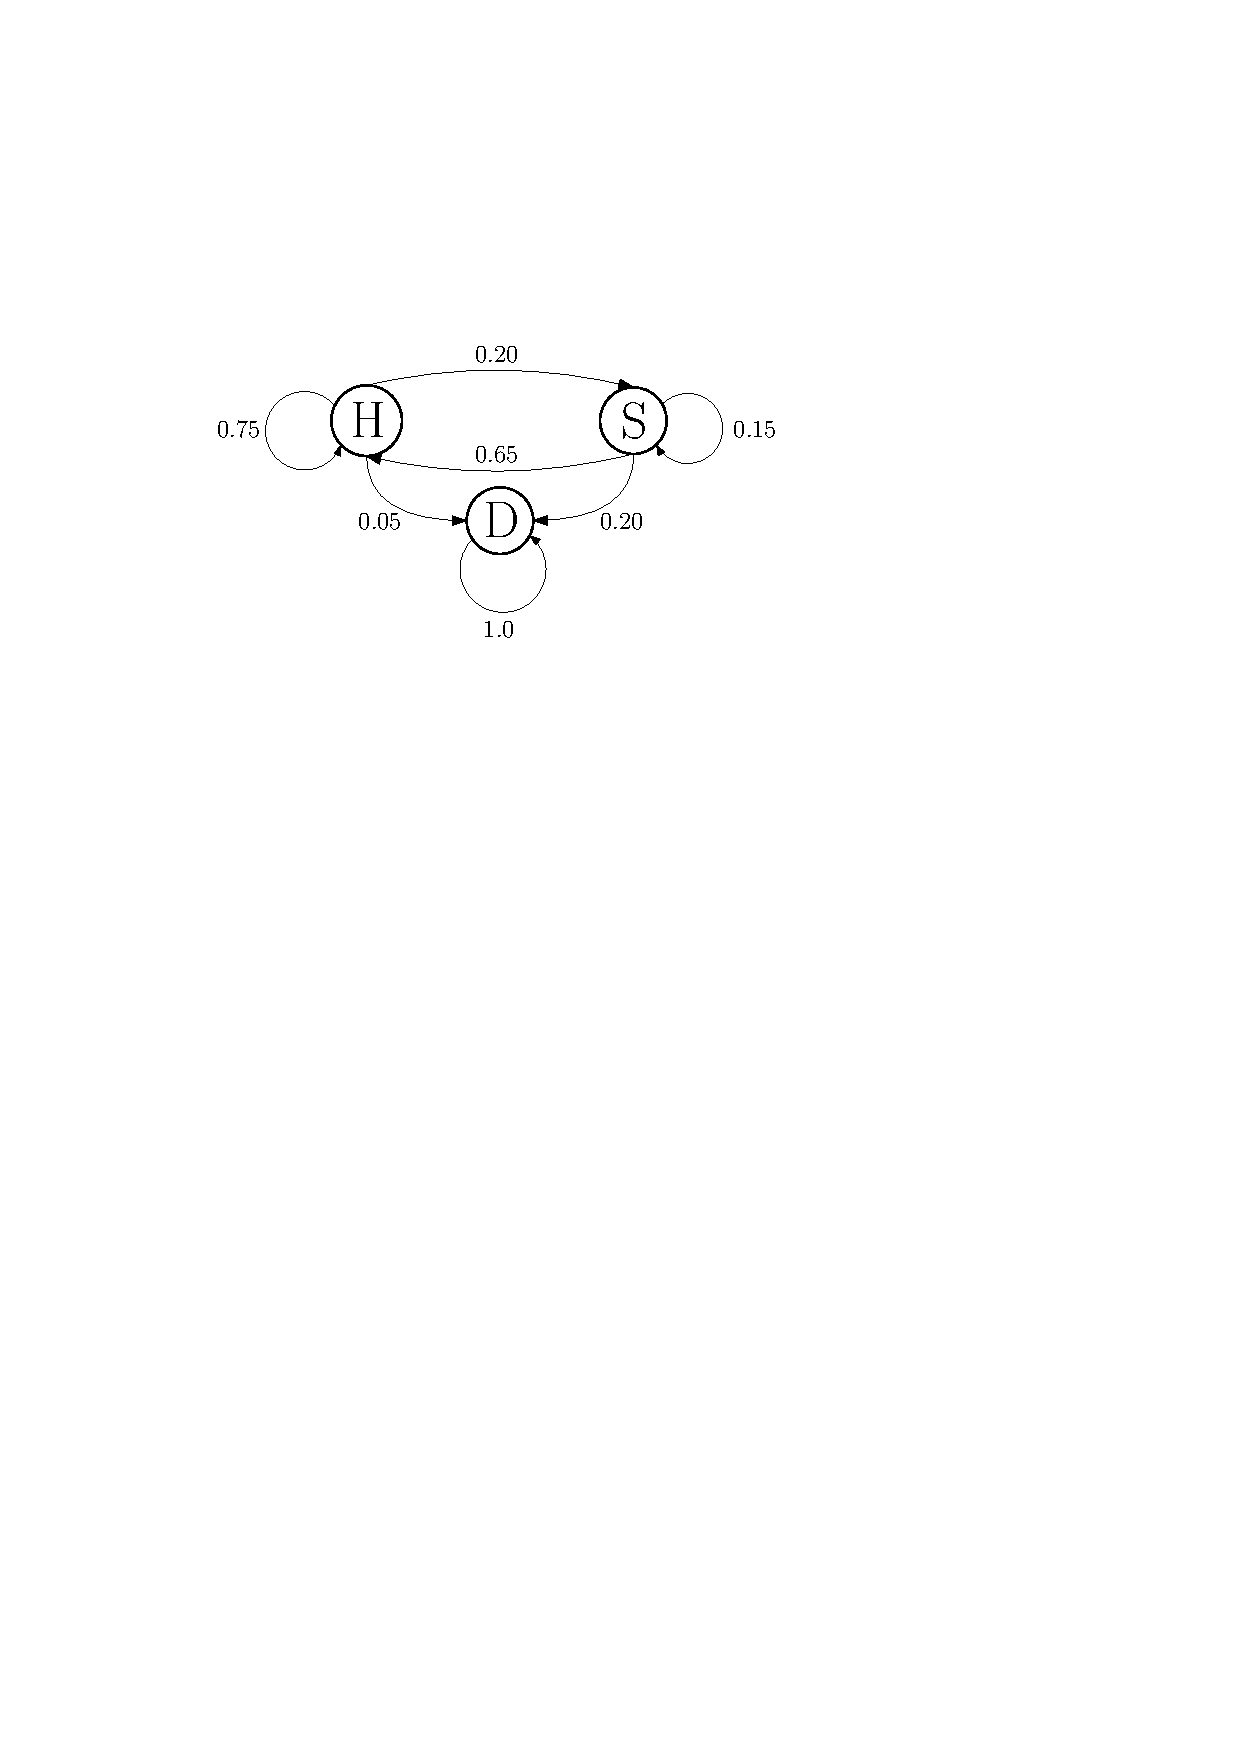
\includegraphics[width=0.9\textwidth]{../figures/chapter5/figures/markov_chain.pdf}
	\caption[Illustration of a $3$-State Markov Chain]{An illustration of a $3$-State Markov chain with the transition probability given by the matrix $P$ in Eq.~(\ref{eq:app_transition_probability_matrix}).}
	\label{fig:app_markov_chain}
\end{figure}

% Marginal Distribution at n-th transition, !!!Citation Needed!!!
The probability A transition from state $x$ to $y$ in one step is given by,
\begin{equation}
	\mathbb{P}(\mathcal{X}^{(i+1)} = y) = \sum_{x \in S} \mathbb{P}(\mathcal{X}^{(i+1)} = y | \mathcal{X}^{(i)} = x) \cdot \mathbb{P}(\mathcal{X}^{(i)} = x)
\label{eq:app_markov_chain_one_step}
\end{equation}
Thus, given those three components, the marginal probability distribution at any given step can be defined.
\marginpar{Marginal distribution of state at step $n$}
Furthermore, the expression can be written in compact form as follows.
For instance $1$-step transition from initial distribution $\pi^{(0)}$ by transition probability matrix $P$ yield the distribution,
\begin{equation}
	\pi^{(1)} = \pi^{(0)} P
\label{eq:app_markov_chain_one_step}
\end{equation}
Where $\pi^{(1)}$ is the probality distribution of states at step $1$.
In general,
\begin{equation}
	\begin{split}
		\pi^{(2)} & = \pi^{(1)} P \\
		          & \vdots \\
		\pi^{(n)} & = \pi^{(n-1)} P \\
		          & = \pi^{(0)} P^n\\
	\end{split}
\label{eq:app_markov_chain_one_step}
\end{equation}
where the $n$-th power of $P$ is called the $n$-step transition probability matrix.
\marginpar{$n$-step transition probability}
In other words, the state at step $n$ is distributed as the $n$-times transition of the initial distribution.
Moreover, due to the stationarity of the transition probability,
this result also holds for an $n$-step transition of a distribution at any starting point,
that is $\pi^{(i+n)} \sim \pi^{(i)} P^{(n)}$.  

% Irreducible Chain, !!!Citation Needed!!!
A Markov chain is said to be \emph{irreducible} if each state in the state space $\mathcal{S}$ can be reached eventually from any other state.
\marginpar{Irreducibility}
Irreducibility is a property of the transition probability matrix $P$ (i.e., having an irreducible transition probability matrix).
Formally,
\begin{equation}
	\forall x, y \in \mathcal{S}, \, \exists n \geq 0 \,\, \text{for which} \,\, p_{x,y}^{(n)} > 0
\label{eq:app_irreducibility}
\end{equation}
Based on this definition the transition matrix of Eq.~(\ref{eq:app_transition_probability_matrix}) is not irreducible as the state of being \emph{Dead} does not allow transition to any of the two other states.
An example of irreducible chain is given in a graphical representation of Fig.~\ref{fig:app_markov_chain_irreducible}.
Note that while state $B$ is not directly connected to state $A$,
the state can eventually be reached from state $B$ through the connection of state $C$ (in this case, $n$ is equal to $2$).
\begin{figure}[bth]
	\centering
	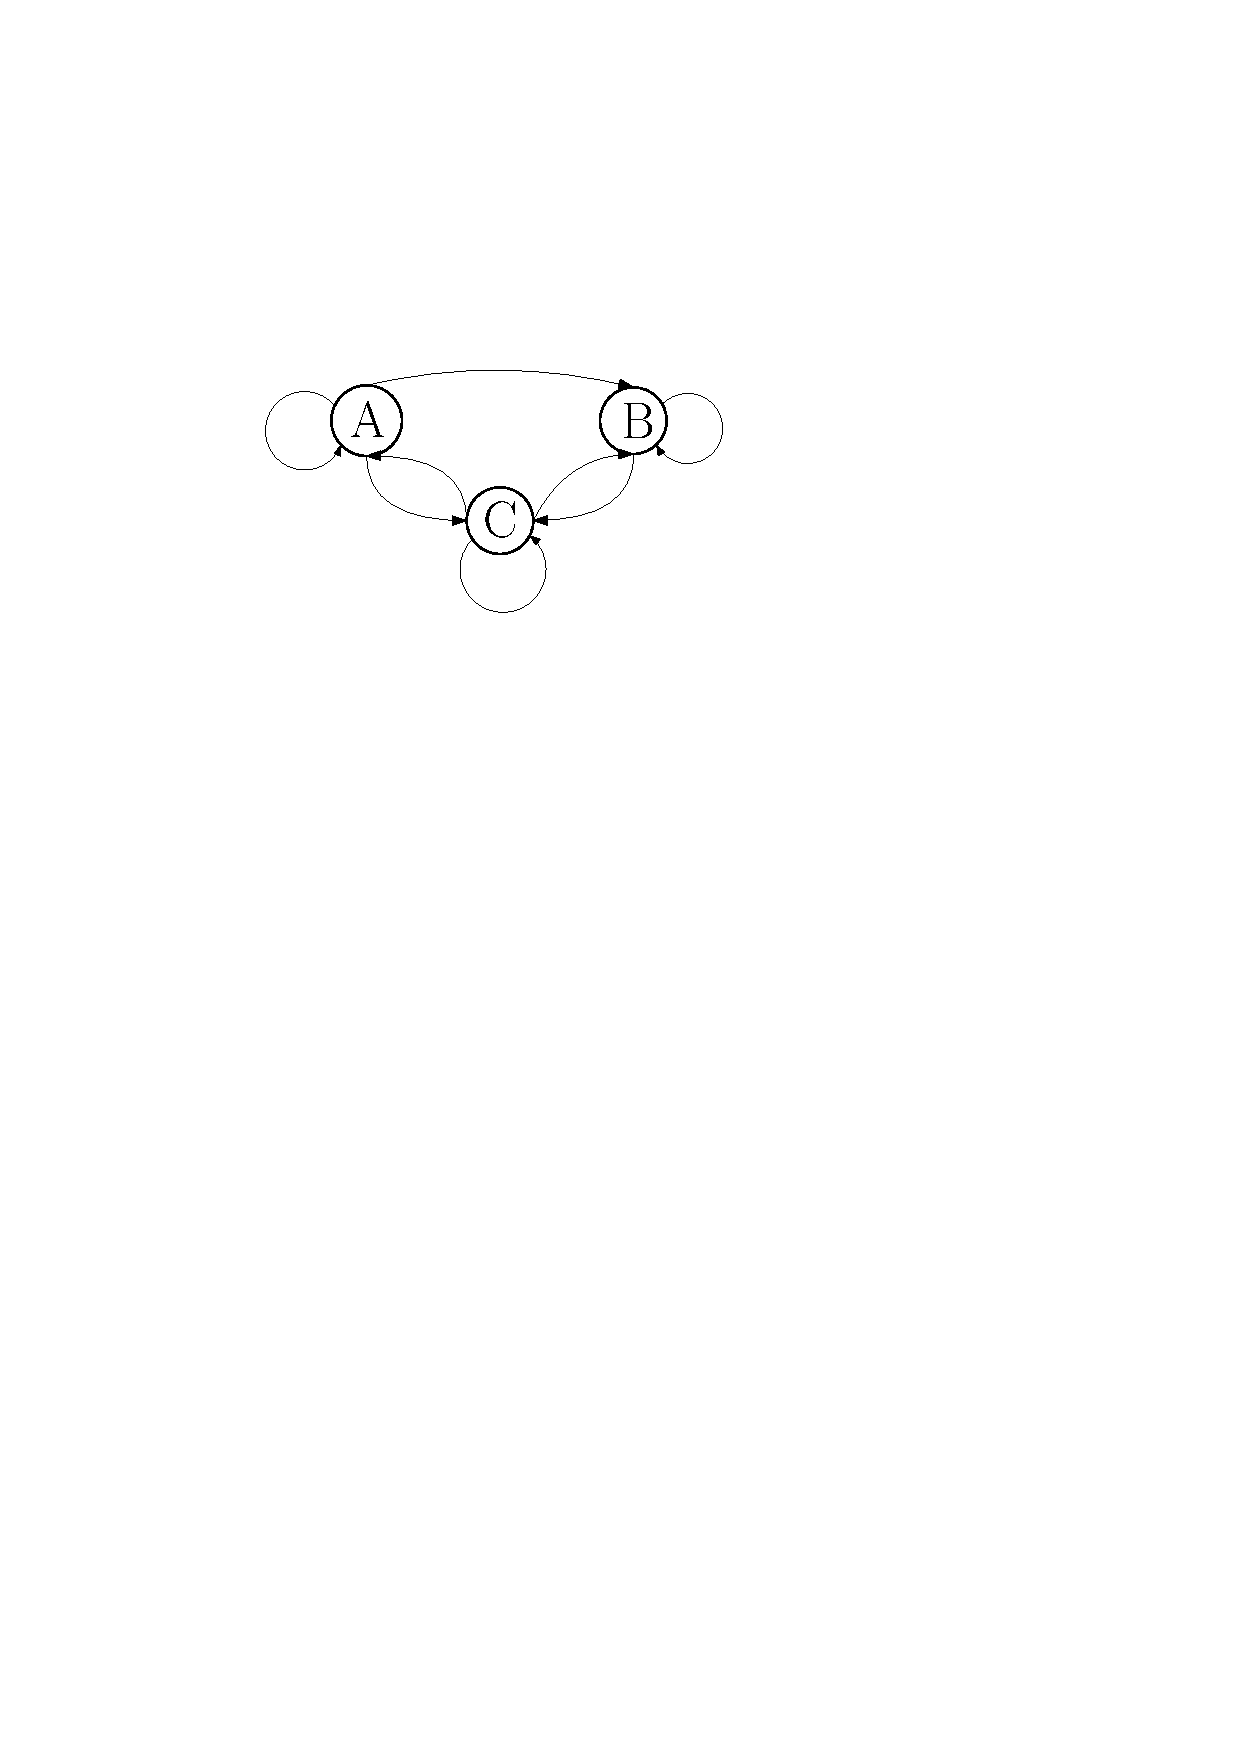
\includegraphics[width=1.0\textwidth]{../figures/chapter5/figures/markov_chain_irreducible.pdf}
	\caption[Illustration of an irreducible $3$-State Markov Chain]{An illustration of an irreducible $3$-State Markov chain.}
	\label{fig:app_markov_chain_irreducible}
\end{figure}

% Period of a Chain and Aperiodicity, !!!Citation Needed!!!
A period of a state $x \in \mathcal{S}$ denoted as $d_x$ is defined for each state in the chain as follow,
\marginpar{period of a state}
\begin{equation}
	d_x = \text{GCD}\,\,\{n: p_{x,x}^{(n)} > 0, n > 0\} \,\, \forall x \in \mathcal{S}
\label{eq:app_markov_chain_period}
\end{equation}
where $\text{GCD}$ stands for the \emph{Greatest Common Divisor} of the set.
In other words, it is the minimum number of transition for any given state to return to the state.

In an arbitrary discrete-state Markov chain, different states might have different periods.
\marginpar{periodic, aperiodic chain}
A state is called \emph{aperiodic} if its period is equal to $1$ and it is called \emph{periodic} otherwise.
If a chain has the same period $d > 1$ for each of its states then the chain is called \emph{periodic} (see Fig.~\ref{fig:app_markov_chain_periodic} for a periodic chain with period $3$).
A periodic chain exhibits a non-stochastic behavior in their dynamic.
On the contrary, a chain having the same period of $1$ for each of its states is called a \emph{aperiodic} chain (see Fig.~\ref{fig:app_markov_chain_aperiodic} for an example of a aperiodic chain).
\normdoublefigure[pos=tbhp,
                  mainlabel={fig:app_markov_chain_periodicity},
                  maincaption={Examples of periodic and aperiodic chains. (Left) an example of a periodic $3$-state Markov chain. In this case, all states have the the same period of $3$ steps. (Right) an example of aperiodic $3$-state Markov chain, that is all states are aperiodic.},%
									mainshortcaption={Examples of periodic and aperiodic chains.},
                  leftopt={width=0.45\textwidth},
                  leftlabel={fig:app_markov_chain_periodic},
                  leftcaption={Periodic chain},
                  %leftshortcaption={},%
                  rightopt={width=0.45\textwidth},
                  rightlabel={fig:app_markov_chain_aperiodic},
                  rightcaption={Aperiodic chain},
                  %rightshortcaption={},
                  %spacing={\hfill}
                 ]
{../figures/chapter5/figures/markov_chain_periodic}
{../figures/chapter5/figures/markov_chain_aperiodic}

% Stationary Distribution, !!!Citation Needed!!!
Some distribution are \emph{stationary} with respect to a transition probability matrix.
\marginpar{Stationary distribution}
Specifically, $\pi^*$ is \emph{stationary for} $P$ if,
\begin{equation}
	\pi^* = \pi^* P
\label{eq:app_markov_chain_stationary}
\end{equation}	
Put differently, the distribution is \emph{invariant} under transition.
Consequently, if stationary distribution exists,
once the chain reaches the stationary distribution, it will remain there and the chain itself becomes stationary. 
Stationary distribution need not exist for a given $P$,
but in the application of \gls[hyper=false]{mcmc} algorithms,
the existence of stationary distribution is guaranteed \cite{Geyer2011}.

% Example of Stationary Distribution
As an example of a stationary distribution, consider once more the transition probability matrix $P$ in Eq.~(\ref{eq:app_transition_probability_matrix}).
For this transition, the distribution $\pi = [0.0, 0.0, 1.0]$ is stationary with respect to $P$ such that
\begin{equation}
	\pi = \pi P \Leftrightarrow [0.0, 0.0, 1.0] = [0.0, 0.0, 1.0] 		\begin{pmatrix}
		  0.75  & 0.20 & 0.05\\
      0.65  & 0.15 & 0.20\\
      0.00  & 0.00 & 1.00\\
		\end{pmatrix}
\label{eq:app_markov_chain_stationary_example}
\end{equation}
Stating that the stationary distribution is being dead, eventually and definitely.

% Markov Chain Convergence
The notions of irreducibility, aperiodicity, and stationarity are cobbled together to arrive at an important result in the discrete-state Markov chain and it is stated here without proof (citation needed).
\marginpar{Fundamental theorem of Markov chain}
Let $P$ be a transition probability matrix, irreducible and aperiodic, then $P$ has exactly one stationary distribution $\pi^*$ and for any initial distribution $\pi^{(0)}$
\begin{equation}
	\lim_{t \rightarrow \infty} |\pi^{(0)}P^t - \pi^*| = 0
\label{eq:app_markov_chain_convergence}
\end{equation}
That is, the chain converges \emph{in distribution} to the stationary distribution regardless its initial distribution.
The theorem also indicates the existence of a \emph{limiting distribution} $\lim_{t \rightarrow \infty} \pi^{(0)}P^t$.

% MCMC Algorithm
The theorem justifies the use of Markov chain to generate samples for Monte Carlo application from an arbitrary distribution of interest.
\marginpar{Markov Chain Monte Carlo}
This is what \gls[hyper=false]{mcmc} algorithms do.
In such an algorithm the task is to come up with transition probability such that the limiting distribution of the Markov chain, over many iterations, converges to the distribution of interest (the so-called \emph{target} distribution).
Stated differently, the stationary distribution of the Markov chain is aimed to be the distribution of interest.

%-----------------------------------------------------
\subsection{Continuous-State}\label{app:mc_continuous}
%-----------------------------------------------------

% Markov Chain

% Ingredients

% Transition Kernel

% Ergodic Theorem

% Some difficulty


%*******************************************************
\section{Karhunen-Lo\'eve Theorem}\label{app:kl_theorem}
%*******************************************************

The Karhunen-Lo\'eve theorem establishes that for any centered mean-square continuous stochastic process $\mathcal{Y}(\circ)$ on a domain $\mathcal{D} \subseteq \mathbb{R}$ defined by a sample space $\Omega$,
there exists a set of basis functions ${\xi_j}$ defined on $\mathcal{D}$ such that for all $t \in \mathcal{D}$,
\begin{equation}
	\mathcal{Y} = \sum_{j=1}^{+\infty} \theta_j \cdot \xi_j(t)
\label{eq:kl_theorem}
\end{equation}

The scalar coefficients $\theta_j$ in Eq.~(\ref{eq:kl_theorem}) are given for each $\omega \in \Omega$ by $\theta_j(\omega) = \int_\mathcal{D} \mathcal{Y}(\omega) \xi_j(t) dt$ and satisfy the following:
\begin{equation}
	\begin{split}
		\mathbb{E}[\theta_j] & = 0 \\
		\mathbb{V}[\theta_j] & = \rho_j \\
    \mathbb{E}[\theta_j\cdot \theta_k] & = \delta_{jk} \rho_j
	\end{split}
\label{eq:kl_condition}
\end{equation}
where $\mathbb{E}[\circ]$ and $\mathbb{V}[\circ]$ are the expectation and the variance operators, respectively;
$\delta$ is the Kronecker delta;
$\rho_j$ is the eigenvalue associate with basis function $\xi_j(t)$.
Eqs.~(\ref{eq:kl_theorem}) and~(\ref{eq:kl_condition}) imply that $\theta_j$ is independent and identically distributed (i.i.d) with mean $0$ and variance $\rho_j$~\cite{Wang2008}.

The basis function, in turn, is defined as the eigenfunction of the functional operator $\mathbb{K}[f(\circ)]$ on some function $f(\circ)$ applied to $\xi_j(t)$
\begin{equation}
	\mathbb{K}[\xi_j(t)] = \int_{\mathcal{D}} R (t, s) \cdot \xi_j(s) ds = \rho_j \cdot \xi_j(t); \, \forall t \in \mathcal{D}
\label{eq:kl_operator}
\end{equation}
where $R (t, s)$ is the covariance function of the stochastic process $\mathcal{Y}$ for the covariance between time $t$ and $s$,
i.e., $R (t, s) \equiv \mathbb{E}[\mathcal{Y}_t \cdot \mathcal{Y}_s]$.

The Karhunen-Lo\'eve theorem is applicable to the functional deviation from the proper mean and therefore allows for each element of the data set to be represented as a series that is optimal in the root-mean-square-of-error sense:
\begin{equation}
	y_n(t) = \bar{y}(t) + \sum_{j=1}^{+\infty} \theta_{j,n} \cdot \xi_j(t); \, n = 1, \dots, N
\label{eq:kl_rmse_optimal}
\end{equation}
where $\xi_j(t)$ is the series of orthogonal eigenfunctions (or \gls[hyper=false]{fpc}),
and the corresponding \gls[hyper=false]{fpc} score $\theta_{j,n}$ associated with each function realization is defined by the orthogonality condition
\begin{equation}
	\theta_{j,n} = \int_{\mathcal{D}} [y_n(t) - \bar{y}(t)] \cdot \xi_j(t) dt
\label{eq:kl_orthogonality}
\end{equation}

As can be seen in Eq.~(\ref{eq:kl_rmse_optimal}), the transformation is exact if the set of eigenfunctions is infinite, but truncation is needed for practical application.
Such details of the actual implementation of \gls[hyper=false]{fpca} can be found in Refs.~\cite{Ramsay2005,Ramsay2014,Wicaksono2014a}.

%********************************************************************
\section{Calibration Score and Informativeness}\label{app:calib_info}
%********************************************************************

% Introductory Paragraph

%********************************************************************
% Other Stuff in the Back
%*******************************************************
\cleardoublepage%********************************************************************
% Bibliography
%*******************************************************
% work-around to have small caps also here in the headline
\manualmark
\markboth{\spacedlowsmallcaps{\bibname}}{\spacedlowsmallcaps{\bibname}} % work-around to have small caps also
%\phantomsection 
\refstepcounter{dummy}
\addtocontents{toc}{\protect\vspace{\beforebibskip}} % to have the bib a bit from the rest in the toc
\addcontentsline{toc}{chapter}{\tocEntry{\bibname}}
\label{app:bibliography}
\printbibliography

\manualmark
\markboth{\spacedlowsmallcaps{Glossaries}}{\spacedlowsmallcaps{Glossaries}} % work-around to have small caps also
%\phantomsection 
\refstepcounter{dummy}
%\addtocontents{gls}{\protect\vspace{\beforebibskip}} % to have the bib a bit from the rest in the toc
%\addcontentsline{gls}{chapter}{\tocEntry{Glossaries}}
\glsaddall
\printglossary[type=\acronymtype,title=Acronyms and Abbreviations]
\label{app:acronyms}
\printglossary[title=Notations (Alphanumeric), type=alphanumeric]
\label{app:notations}
\printglossary[title=Notations (Greek), type=greek]

\cleardoublepage%*****************************************************************************
%\chapter{Glossary}\label{app:glossary}
%*****************************************************************************
%\section*{Nomenclature}\label{nomenclature}
% work-around to have small caps also here in the headline
\manualmark
\markboth{\spacedlowsmallcaps{Glossaries}}{\spacedlowsmallcaps{Glossaries}} % work-around to have small caps also
%\phantomsection 
\refstepcounter{dummy}
%\addtocontents{gls}{\protect\vspace{\beforebibskip}} % to have the bib a bit from the rest in the toc
%\addcontentsline{gls}{chapter}{\tocEntry{Glossaries}}
\glsaddall
\printglossary[type=\acronymtype,title=Acronyms and Abbreviations]
\printglossary[title=Notations (Alphanumeric), type=alphanumeric]
\printglossary[title=Notations (Greek), type=greek]
\cleardoublepage%*******************************************************
% Declaration
%*******************************************************
\refstepcounter{dummy}
\pdfbookmark[0]{Declaration}{declaration}
\chapter*{Declaration}
\thispagestyle{empty}
Put your declaration here.
\bigskip
 
\noindent\textit{\myLocation, \myTime}

\smallskip

\begin{flushright}
    \begin{tabular}{m{5cm}}
        \\ \hline
        \centering\myName \\
    \end{tabular}
\end{flushright}

\cleardoublepage\pagestyle{empty}

\hfill

\vfill


\pdfbookmark[0]{Colophon}{colophon}
\section*{Colophon}
This document was typeset using the typographical look-and-feel \texttt{classicthesis} developed by Andr\'e Miede. 
The style was inspired by Robert Bringhurst's seminal book on typography ``\emph{The Elements of Typographic Style}''. 
\texttt{classicthesis} is available for both \LaTeX\ and \mLyX: 
\begin{center}
\url{https://bitbucket.org/amiede/classicthesis/}
\end{center}
Happy users of \texttt{classicthesis} usually send a real postcard to the author, a collection of postcards received so far is featured here: 
\begin{center}
\url{http://postcards.miede.de/}
\end{center}
 
\bigskip

\noindent\finalVersionString

%Hermann Zapf's \emph{Palatino} and \emph{Euler} type faces (Type~1 PostScript fonts \emph{URW
%Palladio L} and \emph{FPL}) are used. The ``typewriter'' text is typeset in \emph{Bera Mono}, 
%originally developed by Bitstream, Inc. as ``Bitstream Vera''. (Type~1 PostScript fonts were made 
%available by Malte Rosenau and
%Ulrich Dirr.)

%\paragraph{note:} The custom size of the textblock was calculated
%using the directions given by Mr. Bringhurst (pages 26--29 and
%175/176). 10~pt Palatino needs  133.21~pt for the string
%``abcdefghijklmnopqrstuvwxyz''. This yields a good line length between
%24--26~pc (288--312~pt). Using a ``\emph{double square textblock}''
%with a 1:2 ratio this results in a textblock of 312:624~pt (which
%includes the headline in this design). A good alternative would be the
%``\emph{golden section textblock}'' with a ratio of 1:1.62, here
%312:505.44~pt. For comparison, \texttt{DIV9} of the \texttt{typearea}
%package results in a line length of 389~pt (32.4~pc), which is by far
%too long. However, this information will only be of interest for
%hardcore pseudo-typographers like me.%
%
%To make your own calculations, use the following commands and look up
%the corresponding lengths in the book:
%\begin{verbatim}
%    \settowidth{\abcd}{abcdefghijklmnopqrstuvwxyz}
%    \the\abcd\ % prints the value of the length
%\end{verbatim}
%Please see the file \texttt{classicthesis.sty} for some precalculated 
%values for Palatino and Minion.
%
%    \settowidth{\abcd}{abcdefghijklmnopqrstuvwxyz}
%    \the\abcd\ % prints the value of the length





% ********************************************************************
% Game Over: Restore, Restart, or Quit?
%*******************************************************
\end{document}
% ********************************************************************
